% ============================================================================
% Fichier     : ASI_main.tex
% Titre       : Audit des Systèmes d'Information
% Auteur      : MINKA MI NGUIDJOÏ Thierry Emmanuel
% Institution : ENSP Yaoundé — Université de Yaoundé I — LIMSI
% Version     : 0.1 -- octobre 2026 (squelette)
% ============================================================================

\documentclass[12pt, twoside, openright, a4paper]{book}

% --- Feuille de style unifiée ---
\usepackage{Style_ASI}
\raggedbottom  % évite les blancs étirés entre un tableau et sa légende

% --- Bibliographie ---
\addbibresource{bibliographie/ASI_references.bib}

% ============================================================================
% MÉTADONNÉES PDF
% ============================================================================
\hypersetup{
    pdftitle={Audit des Systèmes d'Information},
    pdfauthor={MINKA MI NGUIDJOÏ Thierry Emmanuel},
    pdfsubject={INF3226 · Génie Informatique, niveau 3 · ENSP Yaoundé I},
    pdfkeywords={audit des SI, contrôle interne, gestion des risques, audit de sécurité, audit de conformité, auditologie, NEK}
}

\begin{document}

% --------------------------------------------------------------------------
% ÉLÉMENTS PRÉLIMINAIRES (pages romaines)
% --------------------------------------------------------------------------
\frontmatter

    % ==============================================================================
% Fichier : front/00_page_titre.tex
% Titre   : Page de titre - Audit des Systèmes d'Information
% Auteur  : MINKA MI NGUIDJOÏ Thierry Emmanuel
% Version : 1.0 -- novembre 2026 (charte des cours de l'ENSPY)
% ==============================================================================

\begin{titlepage}
\thispagestyle{empty}

% --- Fond décoratif : bandeaux bleu marine et filets or ---
\begin{tikzpicture}[remember picture, overlay]
    \fill[CouleurPrimaire]
        (current page.north west) rectangle
        ([yshift=-3.6cm] current page.north east);
    \fill[CouleurAccent]
        ([yshift=-3.6cm] current page.north west) rectangle
        ([yshift=-4.0cm] current page.north east);
    \fill[CouleurPrimaire]
        (current page.south west) rectangle
        ([yshift=2.5cm] current page.south east);
    \fill[CouleurAccent]
        ([yshift=2.5cm] current page.south west) rectangle
        ([yshift=2.9cm] current page.south east);
    % En-tête institutionnel, posé dans le bandeau supérieur
    \node[align=center, text=white] at ([yshift=-1.8cm] current page.north) {%
        {\fontsize{11}{13}\selectfont
        \textsc{République du Cameroun}}\\[0.3ex]
        {\color{CouleurAccent!60!white}\rule{0.4\paperwidth}{0.4pt}}\\[0.6ex]
        {\fontsize{10}{12}\selectfont\textbf{\tutelle}}\\[0.2ex]
        {\fontsize{9}{11}\selectfont \institutionprimaire}\\[0.2ex]
        {\fontsize{9}{11}\selectfont \unitepedago}};
    % Logos : Université de Yaoundé I à gauche, ENSPY à droite (cours de l'ENSPY)
    \node[fill=white, rounded corners=4pt, inner sep=2pt]
        at ([xshift=1.75cm, yshift=-1.8cm] current page.north west)
        {
\includegraphics[height=2.6cm]{figures/logos/uy1_logo.png}};
    \node[fill=white, rounded corners=4pt, inner sep=2pt]
        at ([xshift=-1.75cm, yshift=-1.8cm] current page.north east)
        {
\includegraphics[height=2.6cm]{figures/logos/enspy_logo.jpg}};
    % Année et version, posées dans le bandeau inférieur
    \node[align=center] at ([yshift=1.25cm] current page.south) {%
        {\color{white}\bfseries\large Année académique \anneescolaire}\\[0.3ex]
        {\color{CouleurAccent!70!white}\small
        Version 1.0 | Document pédagogique de l'UE \codeUE}};
\end{tikzpicture}

\vspace*{0.6cm}

% --- Titre principal (sur deux lignes) ---
\begin{center}
    {\color{CouleurPrimaire}\rule{0.85\textwidth}{1.2pt}}\\[1.2ex]
    {\fontsize{26}{32}\selectfont\bfseries\color{CouleurPrimaire}
        Audit des Systèmes\\[0.4ex]
        d'Information}\\[0.8ex]
    {\color{CouleurAccent}\rule{0.85\textwidth}{2pt}}\\[0.5ex]
    {\color{CouleurPrimaire}\rule{0.85\textwidth}{0.5pt}}
\end{center}

\vspace{0.8cm}

\begin{center}
    {\fontsize{13}{16}\selectfont\itshape\color{CouleurSecondaire}
        Contrôle interne, risques, sécurité et conformité~:\\
        du métier à l'auditologie}
\end{center}

\vspace{0.5cm}

% --- Cartouche sigle et code UE ---
\begin{center}
    \begin{tikzpicture}
        \node[draw=CouleurPrimaire, fill=CouleurPrimaire, rounded corners=6pt,
              inner xsep=14pt, inner ysep=6pt]{%
            \color{white}\bfseries\large \sigleCours{} - UE~\codeUE
        };
    \end{tikzpicture}
\end{center}

\vspace{1.0cm}

% --- Schéma de la discipline : le gabarit canonique de décomposition, de
%     l'espace d'audit à la trace, lu par les trois mesures µ, U, H ---
\begin{center}
\begin{tikzpicture}[
    niv/.style = {
        draw=CouleurBordDef, fill=CouleurDef, rounded corners=3pt,
        minimum width=2.3cm, minimum height=0.75cm, align=center,
        font=\small\bfseries\color{CouleurPrimaire}, inner sep=2pt
    },
    arrow/.style = {-{Stealth[length=4pt]}, thick, color=CouleurSecondaire}
]
% Ligne 1 : de l'espace audité à l'activité ; ligne 2 : du contrôle à la trace
\foreach \t [count=\i] in {Domaine, Sous-domaine, Processus, Activité} {
    \node[niv] (n\i) at (2.8*\i, 0) {\t};
}
\foreach \t [count=\i from 5] in {Contrôle, Test, Preuve, Trace} {
    \node[niv] (n\i) at (2.8*\i - 11.2, -1.25) {\t};
}
\foreach \i [evaluate=\i as \j using int(\i+1)] in {1,2,3,5,6,7}
    \draw[arrow] (n\i) -- (n\j);
\draw[arrow] (n4.south) -- ++(0,-0.25) -| (n5.north);
\node[draw=CouleurPrimaire, fill=CouleurPrimaire, rounded corners=4pt,
      align=center, font=\footnotesize\bfseries\color{white}, inner xsep=8pt]
      (mes) at (7.0, -2.65)
      {\OUI{} / \NON{} / \NEK{} \quad$\longrightarrow$\quad
       $\mu$ (conformité) · $U$ (incertitude) · $H$ (entropie)};
\draw[arrow] (n6.south) -- (n6.south |- mes.north);
\end{tikzpicture}
\end{center}

\vspace{0.6cm}

\begin{center}
    {\large\bfseries\color{CouleurPrimaire}
        \auteurcours}\\[0.5ex]
    {\normalsize\color{CouleurSecondaire}
       Enseignant Chercheur | \laboratoire{} | ENSPY}\\[0.2ex]
    {\small\color{CouleurBordInfo}
        \institutionprimaire{} · \tutelle}\\[0.2ex]
    {\small\color{CouleurBordInfo}
        \href{mailto:maletyon@proton.me}{maletyon@proton.me}}
\end{center}

\end{titlepage}

    \cleardoublepage

    % ============================================================================
% Fichier  : front/01_avant_propos.tex
% Titre    : Avant-propos
% Auteur   : MINKA MI NGUIDJOÏ Thierry Emmanuel
% Version  : 1.0 -- novembre 2026
% ============================================================================
% Décision du 06/11/2026 : seuls A0 et A1 (HAL) sont cités ; aucun travail
% non publié n'est annoncé. 60 h = 30 séances de 2 h ; 31 chapitres.
% ============================================================================

\chapter*{Avant-propos}
\addcontentsline{toc}{chapter}{Avant-propos}
\markboth{Avant-propos}{Avant-propos}

\epigraph{« Ce que l'organisation ignore de ses propres systèmes conditionne
la qualité des décisions qu'elle peut prendre à leur sujet. »}%
{\textit{Vers l'auditologie}~\cite{minka2026auditologie}}

Pour la plupart des élèves ingénieurs du Département de Génie Informatique
de l'École Nationale Supérieure Polytechnique de Yaoundé, ce cours est le
seul consacré à l'audit, au contrôle interne, à la gestion des risques, à
l'audit de sécurité et à l'audit de conformité. Il est donc
autoportant~: il ne suppose ni cours de gouvernance, ni cours de gestion
des risques préalable. Il prépare aussi aux UE d'investigation numérique
(SEC4031 et SEC4052), qui reprennent là où il s'arrête~: à la preuve.

Il repose sur une double conviction. La première est qu'auditer ne consiste
pas à remplir une grille, mais à réduire l'incertitude d'un tiers sur un
système qu'il ne peut pas observer seul. Un conseil d'administration, un
régulateur, un juge s'appuient sur ce que l'auditeur affirme~; ils doivent
pouvoir savoir aussi ce qu'il ignore. C'est pourquoi ce cours admet, à côté
de \OUI{} et de \NON{}, une troisième réponse~: \NEK{}, « connaissance
insuffisante ».

La seconde conviction est que le métier ne s'importe pas tel quel. Les
normes de l'IIA, de l'ISACA, de l'ISO et de l'INTOSAI sont des acquis
précieux~; elles s'appliquent ici sous le regard de la loi camerounaise sur
la cybersécurité et la cybercriminalité, de la COBAC, du droit OHADA et de
la Chambre des comptes, dans des organisations dont les moyens et les
contraintes sont les nôtres.

\bigskip

\textbf{Ce que ce cours n'est pas.} Il n'est pas un résumé des normes
professionnelles, ni une préparation à une certification, ni un cours de
tests d'intrusion. Les normes y sont citées avec exactitude, dans l'édition
en vigueur quand elle a pu être vérifiée~; les textes de loi n'y sont cités
entre guillemets que s'ils ont été lus dans leur version officielle.

\bigskip

\textbf{Ce que ce cours est.} Un traité de trente et un chapitres, en six
parties précédées d'un prologue, qui va du cas concret vers la méthode, de
la méthode vers la pratique, et de la pratique vers la recherche. La
Partie~I pose les fondements~: audit, contrôle interne, risque et sa
gestion, fraude. La Partie~II donne la méthode de la mission, de la lettre
de mission au suivi. La Partie~III présente les normes, les référentiels,
le droit et la déontologie. La Partie~IV audite le système d'information
domaine par domaine, de la gouvernance à la conformité, en passant par la
sécurité, les tests d'intrusion, la continuité et les tiers, et se termine
par trois cas intégrateurs. La Partie~V aborde l'audit continu,
l'intelligence artificielle et le passage de l'audit à la preuve
judiciaire. La Partie~VI présente le programme de recherche sur lequel la
méthode s'appuie.

\bigskip

\textbf{Un cours, un corpus.} La méthode enseignée est l'instanciation
opérationnelle, pour le praticien, du programme de recherche de
l'auditologie~\cite{minka2026auditologie}~; son instrument de réponse
\OUI{}~/ \NON{}~/ \NEK{} et ses mesures viennent de l'article
\cite{minka2026nek}. Ces deux textes sont des prépublications déposées sur
HAL, et le cours les cite comme telles. Les autres appuis sont des travaux
publiés et vérifiables~: théorie de l'information, théorie des jeux,
psychologie cognitive, métrologie, normes professionnelles. Ce cours est la
version complète du corpus~; le cours ACSI du Master de la Chaire UNESCO en
est une version resserrée.

\bigskip

\textbf{Trois organisations fictives.} Le cours suit trois missions.
\emph{LiZbiZ}, entreprise de logistique aux quatre centres de données,
reprise de l'article fondateur, est le cas principal~: le cabinet AUDIX
CONSEIL y conduit deux cycles d'audit. La \emph{BANQUE SANAGA}, à Douala,
affronte les suites d'une panne et le regard de la COBAC. L'\emph{ANPP},
agence publique de paiement, est auditée par la Chambre des comptes. Les
noms, les dates et les montants sont fictifs~; les situations sont
plausibles, et chaque chiffre se recalcule.

\bigskip

\textbf{Comment travailler.} Lisez chaque chapitre avec sa fiche
d'auto-évaluation~; refaites les calculs des lectures auditologiques~;
faites les labs de NDAP SUKULU avant d'en lire les corrigés. Surtout,
prenez l'habitude que le cours cherche à transmettre~: séparer ce que l'on
a constaté de ce que l'on en pense, et dire ce que l'on ne sait pas.

\bigskip

\begin{flushright}
    \textit{\auteurcours}\\
    \textit{Yaoundé, novembre 2026}
\end{flushright}

    \cleardoublepage

    % ============================================================================
% Fichier  : front/02_mode_emploi.tex
% Titre    : Mode d'emploi du cours
% Auteur   : MINKA MI NGUIDJOÏ Thierry Emmanuel
% Version  : 1.0 -- novembre 2026
% ============================================================================
% 60 h = 30 séances de 2 h (norme des cours ENSPY) ; fiches et labs hors
% de ces 60 h.
% ============================================================================

\chapter*{Mode d'emploi du cours}
\addcontentsline{toc}{chapter}{Mode d'emploi du cours}
\markboth{Mode d'emploi}{Mode d'emploi}

\section*{Structure générale}

Le cours compte un prologue et six parties, soit 31~chapitres, pour
60~heures en présentiel réparties en trente séances de deux heures. Les
fiches d'auto-évaluation par chapitre et les laboratoires de 60~minutes de
NDAP SUKULU sont des travaux à faire hors de ces 60~heures. Les Parties~V
et~VI servent en outre de point de départ aux projets et aux mémoires.

\begin{tableaucours}{L{1.6cm}L{4.4cm}L{4.4cm}L{1.8cm}}{%
    \tableauHeader{Partie} &
    \tableauHeader{Thème} &
    \tableauHeader{Compétences visées} &
    \tableauHeader{Niveau}
}
Prologue & Quarante-cinq questions & Distinguer constatation, impression et
opinion & \niveaubase \\
I & Fondements de l'audit, du contrôle et du risque & Situer l'audit,
évaluer un contrôle, mesurer et gérer un risque, repérer la fraude &
\niveaubase \\
II & Méthode de la mission & Planifier, décomposer, collecter la preuve,
conclure avec $\mu$, $U$ et $H$, suivre & \niveaumoyen \\
III & Cadre normatif, juridique et déontologique & Choisir ses normes et
ses critères~; connaître ses obligations et ses devoirs & \niveaubase \\
IV & Pratique de l'audit des SI & Auditer la gouvernance, une application,
un projet, la sécurité, la continuité, les tiers, la conformité &
\niveaumoyen{} à \niveauexpert \\
V & Défis avancés & Audit continu, IA, passage à la preuve judiciaire &
\niveauexpert \\
VI & Recherche~: l'auditologie & Lire et prolonger le programme de
recherche & \niveauexpert \\
\end{tableaucours}

\section*{Les trente séances}

\begin{tableaucours}{L{1.4cm}L{7.4cm}L{3.4cm}}{%
    \tableauHeader{Séance} &
    \tableauHeader{Contenu} &
    \tableauHeader{Partie}
}
1 & Prologue~: quarante-cinq questions & Prologue \\
2 & Auditer, contrôler, donner une assurance (Ch.~\ref{chap:audit-auditologie}) & I \\
3 & Grandes défaillances (Ch.~\ref{chap:defaillances}) & I \\
4 & Le contrôle interne (Ch.~\ref{chap:controle-interne}) & I \\
5 & Le risque, notions et mesure (Ch.~\ref{chap:risque}) & I \\
6 & Gérer les risques des SI (Ch.~\ref{chap:gestion-risques}) & I \\
7 & La fraude (Ch.~\ref{chap:fraude}) & I \\
8 & La mission d'audit (Ch.~\ref{chap:mission}) & II \\
9 & Préparer et planifier (Ch.~\ref{chap:planifier}) & II \\
10 & Décomposer l'espace d'audit (Ch.~\ref{chap:decomposition}) & II \\
11 & Collecter la preuve (Ch.~\ref{chap:preuve}) & II \\
12 & Conclure et rédiger (Ch.~\ref{chap:conclure}) & II \\
13 & Suivre (Ch.~\ref{chap:suivi}) & II \\
14 & Les normes professionnelles (Ch.~\ref{chap:normes}) & III \\
15 & Les référentiels de contrôle (Ch.~\ref{chap:referentiels}) & III \\
16 & Le cadre juridique (Ch.~\ref{chap:droit}) & III \\
17 & Déontologie et profession (Ch.~\ref{chap:deontologie}) & III \\
18 & Gouvernance et fonction informatique (Ch.~\ref{chap:audit-gouvernance}) & IV \\
19 & Une application en service (Ch.~\ref{chap:audit-applications}) & IV \\
20 & Les projets informatiques (Ch.~\ref{chap:audit-projets}) & IV \\
21 & Le système de management de la sécurité (Ch.~\ref{chap:audit-smsi}) & IV \\
22 & La sécurité technique (Ch.~\ref{chap:audit-technique}) & IV \\
23 & Tests d'intrusion et audit de code (Ch.~\ref{chap:intrusion}) & IV \\
24 & Production et continuité (Ch.~\ref{chap:audit-continuite}) & IV \\
25 & Les tiers et le nuage (Ch.~\ref{chap:audit-tiers}) & IV \\
26 & La conformité (Ch.~\ref{chap:audit-conformite}) & IV \\
27 & Études de cas intégratrices (Ch.~\ref{chap:cas-integrateurs}) & IV \\
28 & Audit continu~; auditer l'IA (Ch.~\ref{chap:audit-continu}
et~\ref{chap:audit-ia}) & V \\
29 & De l'audit à la preuve judiciaire (Ch.~\ref{chap:audit-preuve}) & V \\
30 & L'auditologie~; mesurer l'incertitude (Ch.~\ref{chap:auditologie}
et~\ref{chap:incertitude}) & VI \\
\end{tableaucours}

\section*{Les encadrés}

\begin{boxdef}
\textbf{Définition}. Introduit un terme avec sa définition~; les termes
définis sont indexés et repris dans le glossaire (Annexe~\ref{ann:glossaire}).
\end{boxdef}

\begin{boxscenario}{Titre du scénario}
\textbf{Scénario opérationnel}. Un épisode d'une des trois opérations du
cours~: LIZBIZ, SANAGA, MEFOU.
\end{boxscenario}

\begin{boxlecture}{Titre de la lecture}
\textbf{Lecture auditologique}. Une cotation \OUI{}~/ \NON{}~/ \NEK{}, sa
constatation, son analyse avec un niveau de confiance, et les trois mesures
du domaine, rappelées en bas à droite.

\medskip
\hfill\lecture{0{,}65}{0{,}25}{1{,}24}
\end{boxlecture}

\begin{boxobjet}{Code · Intitulé}
\textbf{Fiche d'assertion}. Présente un contrôle sous une forme
constante~: objectif, critère, question, risque, conséquence, puis test,
preuve et trace~; ou une observation en sept éléments.
\end{boxobjet}

\begin{boxprocedure}
\textbf{Papier de travail}. Dit ce que l'auditeur doit faire, et ce que le
dossier doit contenir, pour qu'une étape soit opposable.
\end{boxprocedure}

\begin{boxmetier}{Auditeur SI}
\textbf{Application métier}. Traduit le chapitre en gestes concrets pour
l'un des métiers visés~: auditeur SI, contrôleur interne, auditeur de
sécurité, RSSI, gestionnaire de risques, responsable de la conformité.
\end{boxmetier}

\begin{boxoutils}{Titre de l'outil}
\textbf{Outils}. Un programme, une requête ou une commande, à refaire sur
les données du cas.
\end{boxoutils}

\begin{boxjuris}
Cite un texte de loi ou de règlement, avec son degré de vérification, puis
en tire la portée pour l'audit.
\end{boxjuris}

\begin{boxalert}
\textbf{Violation typique} et \textbf{règle}~: une erreur fréquente, et ce
qu'il faut faire à la place.
\end{boxalert}

\begin{boxresume}
\textbf{À retenir}. Les points essentiels du chapitre.
\end{boxresume}

\begin{boxexo}
\textbf{Exercice}. Dix par chapitre, gradués en trois niveaux~:
\niveaubase\ fondamental, \niveaumoyen\ intermédiaire, \niveauexpert\
expert. Les corrigés figurent dans le livret de correction.
\end{boxexo}

\section*{Conventions}

\begin{itemize}
    \item Les réponses s'écrivent \OUI{}, \NON{} et \NEK{}~; un contrôle sans
          objet est écarté, raison écrite, et n'entre pas dans les calculs.
    \item $\mu$ est le taux de conformité, $U$ le taux d'incertitude, $H$
          l'entropie en bits (au plus $\log_2 3 \approx 1{,}585$)~; la règle
          de décision examine $U$ d'abord, $\mu$ ensuite, $H$ pour contrôler.
    \item Les seuils du quadrant ($\mu = 0{,}5$~; $U = 0{,}20$) et la
          conversion en niveaux de maturité sont des conventions
          pédagogiques, déclarées comme telles.
    \item Les axiomes de l'auditologie portent la numérotation de l'article
          A0 (Chapitre~\ref{chap:auditologie}).
    \item Chaque analyse indique un niveau de confiance~: faible, moyenne ou
          élevée.
    \item Les \termecle{termes clés} apparaissent en gras~; les normes
          s'écrivent \norme{ISO/IEC~27001}, les lois camerounaises
          \loicam{n°~2010/012}.
\end{itemize}

\section*{Matériel d'accompagnement}

\begin{itemize}
    \item \textbf{Annexes}~: glossaire, référentiel des outils, modèles et
          grilles, textes juridiques et normatifs, bibliographie commentée,
          contacts (Annexes~\ref{ann:glossaire} à~\ref{ann:contacts}).
    \item \textbf{Livret de correction}~: corrigés des exercices et des
          fiches, réservé au formateur.
    \item \textbf{NDAP SUKULU}~: fiches d'auto-évaluation et laboratoires,
          présentés dans la section qui suit ce mode d'emploi.
\end{itemize}

    \cleardoublepage

    % ==============================================================================
% Fichier : front/03_ndap_sukulu.tex
% Titre   : NDAP SUKULU, l'environnement compagnon du cours
% Auteur  : MINKA MI NGUIDJOÏ Thierry Emmanuel
% Version : 1.0 -- novembre 2026
% ==============================================================================
% Texte commun aux cours de l'auteur ; seul le tableau des labs est propre au
% cours (fichier front/03b_labs.tex).
% ==============================================================================

\chapter*{NDAP SUKULU, la salle de classe compagnon}
\addcontentsline{toc}{chapter}{NDAP SUKULU, la salle de classe compagnon}
\markboth{NDAP SUKULU}{NDAP SUKULU}

\begin{center}
    
\includegraphics[width=0.62\textwidth]{figures/logos/logo_ndap_sukulu.png}
\end{center}

\section*{Un nom venu du pays bassa}

\begin{quote}\itshape
Le soir tombe sur Éséka. Un enfant revient des champs avec son grand-père et
lui demande pourquoi il doit marcher si loin, chaque matin, pour aller à
l'école. Le vieil homme s'arrête au bord du chemin et répond, en bassa~:
« \textup{Ndap sukulu}, la salle de classe, ce ne sont pas les murs. Ce sont
les murs qui viennent après. La salle de classe, c'est l'endroit où quelqu'un
t'attend pour t'apprendre ce qu'il sait. » L'enfant insiste~: « Et qui
m'attend~? » Le grand-père sourit~: « \textup{Malet yon}. Ton enseignant. »
\end{quote}

En bassa, la langue paternelle de l'auteur, \textbf{\textit{ndap sukulu}}
désigne la salle de classe et \textbf{\textit{malet yon}} signifie « ton
enseignant ». L'environnement compagnon de ce cours porte ce nom parce qu'il
prolonge la salle de classe au-delà des heures de cours~: il attend
l'étudiant le soir, le week-end, à distance, avec des questions, des pièces à
examiner et une correction immédiate. Il est édité par \textbf{MaletYon},
« ton enseignant », et mis à la disposition des étudiants et des praticiens
qui souhaitent se perfectionner (\href{mailto:maletyon@proton.me}{maletyon@proton.me}).

\section*{Ce que l'on y trouve}

\begin{itemize}
    \item \textbf{Une fiche d'auto-évaluation par chapitre.} Chaque fiche
          puise vingt questions dans une banque de quarante (QCM, vrai ou
          faux, textes à trous). Elle dure trente minutes~; la copie validée
          est verrouillée et notée aussitôt. Le seuil de réussite est de
          60~\%.
    \item \textbf{Des laboratoires pratiques.} Chaque lab place l'étudiant
          devant les pièces d'une affaire du fil rouge (tableurs, journaux,
          contrats, procès-verbaux) dans un bureau d'analyste virtuel,
          ouvert dans le navigateur. Il dure soixante minutes, se termine
          par des points de contrôle notés automatiquement et renvoie aux
          sections du livre qu'il mobilise.
    \item \textbf{Un suivi pour l'enseignant}~: rapport de classe, notes par
          fiche et par lab, journal d'activité.
\end{itemize}

Les fiches et les labs sont des travaux à faire hors des heures de cours.
Ils ne remplacent ni le livre ni les exercices de fin de chapitre~: ils en
vérifient la maîtrise.

\section*{Comment y travailler}

\begin{enumerate}
    \item Se connecter au portail NDAP SUKULU avec ses identifiants et le
          code de cours \textbf{\codeUE}.
    \item Pour un lab, commencer par vérifier l'empreinte SHA-256 des pièces
          (\texttt{sha256sum -c MANIFESTE\_SHA256.txt}), puis travailler sur
          la copie du dossier \texttt{travail}~: les pièces originales sont
          en lecture seule et l'activité est journalisée, comme dans une
          vraie mission.
    \item Lire le rappel de cours affiché par le lab et relire les sections
          citées avant de répondre.
\end{enumerate}

\begin{boxinfo}
\textbf{Si le portail n'est pas encore ouvert.} En attendant le déploiement
de NDAP SUKULU, les fiches de questions sont fournies au format texte dans le
dossier \texttt{fiches} du cours, prêtes à être distribuées. Les corrections
des fiches figurent dans le livret de correction, à la suite des corrigés des
exercices de chaque chapitre.
\end{boxinfo}

\section*{Les laboratoires du cours}

% Tableau des labs du cours ASI (INF3226) dans NDAP SUKULU (propre au cours).
Le cours compte dix laboratoires, disponibles sous le code \codeUE. Le dernier
réunit les trois cas du fil rouge et sert de synthèse.

\begin{tableaucours}{L{2.4cm}L{6.0cm}L{1.6cm}L{2.0cm}}{%
    \tableauHeader{Lab} &
    \tableauHeader{Sujet} &
    \tableauHeader{Chapitre} &
    \tableauHeader{Opération}
}
ASI-LAB-01 & Construire la cartographie des risques & \ref{chap:risque} & LIZBIZ \\
ASI-LAB-02 & Analyser la matrice des droits & \ref{chap:controle-interne} & LIZBIZ \\
ASI-LAB-03 & Coter les documents sollicités, dimensionner les échantillons &
\ref{chap:planifier} & LIZBIZ \\
ASI-LAB-04 & Contrôler une décomposition du domaine D & \ref{chap:decomposition} &
LIZBIZ \\
ASI-LAB-05 & Mesurer, situer et comparer les domaines & \ref{chap:conclure} & LIZBIZ \\
ASI-LAB-06 & Audit de conformité des paiements & \ref{chap:droit} & MEFOU \\
ASI-LAB-07 & Tests substantifs sur les données & \ref{chap:audit-applications} &
LIZBIZ \\
ASI-LAB-08 & Audit d'infrastructure des quatre centres & \ref{chap:audit-technique}
& LIZBIZ \\
ASI-LAB-09 & Auditer la continuité du système central & \ref{chap:audit-continuite}
& SANAGA \\
ASI-LAB-10 & Synthèse des trois cas & \ref{chap:cas-integrateurs} & les trois \\
\end{tableaucours}
\vspace{-0.8em}
\begin{center}{\small\itshape Les laboratoires du cours dans NDAP SUKULU}\end{center}


    \cleardoublepage

    \tableofcontents
    \cleardoublepage

    \listoffigures
    \listoftables
    \cleardoublepage

% CORPS (pages arabes)
% Numérotation des chapitres CONTINUE sur tout le cours : le prologue est le
% chapitre 0, puis C01 à C21, un numéro par fichier.
% --------------------------------------------------------------------------
\mainmatter

    % ======================================================================
    % PARTIE 0 — PROLOGUE OPÉRATIONNEL
    % « Une grille qui ne laisse pas répondre « je ne sais pas » produit des certitudes fausses. »
    % Standards de référence : Aucun standard : un cas qui échoue (illustration d'A0).
    % Niveau : introductif
    % ======================================================================
    \part*{Prologue Opérationnel}
    \addcontentsline{toc}{part}{Prologue Opérationnel}

        \setcounter{chapter}{-1}
        \IfFileExists{partie0/P00_quarante_cinq_questions.tex}{% ============================================================================
% Fichier  : partie0/P00_quarante_cinq_questions.tex
% Titre    : Prologue -- Quarante-Cinq Questions et Aucune Réponse Fiable
% Auteur   : MINKA MI NGUIDJOÏ Thierry Emmanuel
% Version  : 1.0 -- novembre 2026
% ============================================================================
% Source du cas : illustration LizbiZ de l'article A0, « Vers l'auditologie »
% (HAL hal-05701007), section 4. Faits d'A0 à ne pas modifier : grille de 45
% éléments en 5 domaines, domaine D incohérent, H ~ 1,2 bit, décomposition
% 5 x 5, usage stratégique de NEK, régression de 35 % à 18 mois, H ~ 0,6 et
% conformité de 52 % à 84 % six mois plus tard.
% Faits communs avec ACSI (MSN-2S3-MSI05), à garder identiques : P00 (13/2/5,
% binaire 16/20), C07 (D.1 à D.5 : 4/0/0, 1/1/2, 4/0/0, 2/0/2, 2/1/1),
% C08 (PT-14 : 31 départs, 19 / 7 / 5), C09 (A 16/3/1, B 8/3/1, C 1/10/1,
% E 8/6/6 ; novembre D 18/1/1, D_KL 0,26).
% Corrigés des exercices : livret séparé (corriges/Corr_P00.tex).
% ============================================================================

\chapter[Prologue : Quarante-Cinq Questions]{Prologue : Quarante-Cinq Questions et Aucune Réponse Fiable}
\label{chap:prologue}
\chaptermark{Prologue}

\epigraph{%
    « Une grille qui interdit de répondre \emph{je ne sais pas}\\
    ne supprime pas l'ignorance~: elle la déguise en certitude. »%
}{Thierry Minka, auditeur des systèmes d'information}

\niveauChapitre{Introductif}{%
    Aucun prérequis d'audit. Il suffit de savoir calculer une proportion et
    un logarithme. Ce prologue se lit avant toute définition~: il part
    d'une mission qui a échoué.%
}

\begin{boxobjectifs}
\begin{itemize}
    \item Reconstituer, à partir de ses traces, la chronologie d'une mission
          d'audit qui a échoué (opération LIZBIZ).
    \item Distinguer une impression, une constatation et une opinion
          d'audit, et reconnaître chacune dans un rapport.
    \item Identifier les défauts de méthode qui privent un rapport de toute
          valeur probante.
    \item Expliquer pourquoi une grille binaire \OUI{}/\NON{} produit des
          réponses incohérentes sur un système partiellement observable, et
          estimer le biais qu'elle introduit.
    \item Identifier les trois états de connaissance d'une réponse et
          utiliser la modalité \NEK{} (connaissance insuffisante).
    \item Calculer, pour un ensemble de réponses, le taux de conformité~$\mu$,
          le taux d'incertitude~$U$ et l'entropie~$H$, et savoir pourquoi on ne
          conclut jamais sur une seule de ces mesures.
    \item Énoncer les cinq réflexes de l'auditeur et le contenu minimal d'un
          papier de travail.
    \item Situer le cours~: sa méthode, ses trois cas, ses six parties, ses
          quinze travaux pratiques et le projet individuel.
\end{itemize}
\end{boxobjectifs}

\bigskip

% ============================================================================
\section*{Avant de commencer : un rapport que personne n'a voulu signer}
% ============================================================================

Douala, mardi 14~avril~2026, 9~heures. Dans la salle du conseil de
LiZbiZ~SA\footnote{La société LiZbiZ, ses dirigeants, ses prestataires, les
dates et les montants de ce cas sont fictifs. Les mécanismes d'audit, les
normes et les textes cités sont exacts. Le cas reprend l'illustration de
l'article \emph{Vers l'auditologie}~\cite{minka2026auditologie}, dont les
données sont conservées.}, le comité de direction a devant lui un rapport
d'audit de vingt-huit pages. Il a été commandé deux mois plus tôt, dans
l'urgence. Personne, autour de la table, ne veut le signer.

LiZbiZ est une entreprise de logistique. Elle stocke, achemine et livre des
marchandises pour le compte de ses clients, des importateurs et des
distributeurs, dans tout le pays. Son activité repose entièrement sur une
application intégrée, que les agences utilisent pour enregistrer les
entrées en entrepôt, préparer les expéditions, facturer et payer les
fournisseurs.

\begin{tableaucours}{L{4.0cm}L{8.2cm}}{%
    \tableauHeader{Élément} &
    \tableauHeader{Description}
}
Activité & Logistique~: entreposage, transport, livraison, pour le compte
de clients \\
Implantation & Siège à Douala~; douze agences régionales \\
Informatique & Quatre centres de données (Douala, Yaoundé, Garoua,
Bafoussam)~; une application intégrée commune à toutes les agences \\
Fonctions de l'application & Stocks et entrepôts~; expéditions~;
facturation~; achats et paiements des fournisseurs \\
Volume (exercice 2025) & 18\,340 expéditions livrées~; 4\,812 paiements
fournisseurs \\
Direction & M.~ETEME, directeur général~; Mme~NKENG, contrôleuse interne~;
M.~KOUNOU, responsable informatique \\
Commissaire aux comptes & Cabinet NDONGO \& ASSOCIÉS \\
\end{tableaucours}
\vspace{-0.8em}
\begin{center}{\small\itshape Tableau~P.1. Fiche d'identité de LiZbiZ}\end{center}

La mission était née de deux alertes. L'inventaire annuel des entrepôts a
fait apparaître un écart de \textbf{186~millions de francs CFA} entre le
stock enregistré dans l'application et le stock compté physiquement. Le
commissaire aux comptes a assorti sa certification des comptes d'une
réserve sur les stocks~: il n'a pas pu s'assurer que le chiffre inscrit au
bilan était juste. Le directeur général a alors demandé un audit «~de tout
le système d'information, et vite~».

L'équipe d'audit interne a travaillé avec une grille de \textbf{45~questions}
réparties en \textbf{5~domaines}, à cocher OUI ou NON. Les réponses ont été
recueillies auprès du responsable informatique, des chefs d'agence et des
responsables des centres de données. Le rapport conclut que le contrôle
d'accès à l'application est «~globalement maîtrisé~».

Le commissaire aux comptes en a demandé les papiers de travail. Il n'y en a
pas. Le responsable informatique conteste deux conclusions. Trois chefs
d'agence affirment n'avoir jamais été interrogés sur les points qu'on leur
attribue. Le comité refuse de valider le rapport.

\medskip

Ce prologue reconstitue cet échec, en cherche les causes, puis suit la
mission qui l'a repris. Il en tire les réflexes qui structurent tout le
cours. Il ne suppose aucune connaissance préalable~: les notions sont
nommées ici, et définies avec précision dans les chapitres qui suivent.

\begin{boxalert}
\textbf{Violation typique.} Conclure «~globalement maîtrisé~» sur un domaine
où les répondants se contredisent, sans avoir noté qui a répondu quoi, ni
sur quelle preuve.

\smallskip
\textbf{Règle~:} une conclusion d'audit qui ne peut pas être reliée à une
preuve conservée n'est pas une conclusion~: c'est une opinion personnelle.
\end{boxalert}

\separateur

% ============================================================================
\section{Ce qui s'est passé}
\label{sec:pro-chronologie}
% ============================================================================

\subsection{Reconstituer avant de juger}

Un ingénieur qui analyse une panne ne commence pas par chercher un
coupable~: il reconstitue la séquence des événements à partir des journaux.
L'auditeur fait de même avec une mission qui a échoué. Il rassemble les
traces disponibles (courriels, versions successives du rapport, comptes
rendus de réunion, fichiers de travail) et les ordonne. Il ne retient que ce
qu'une trace atteste~; ce qu'on lui raconte sans trace reste une
déclaration, à vérifier.

Mme~NKENG, la contrôleuse interne, a établi la chronologie du
Tableau~P.2 après le refus du comité. Chaque ligne y est rattachée à une
pièce.

\begin{tableaucours}{L{2.4cm}L{6.6cm}L{3.2cm}}{%
    \tableauHeader{Date} &
    \tableauHeader{Événement} &
    \tableauHeader{Pièce}
}
12 février 2026 & Le directeur général demande un audit « de tout le système
d'information » par courriel, sans objectifs, ni périmètre, ni référentiel
& Courriel du DG \\
16 février & L'équipe reprend une grille de 45 questions utilisée dans une
autre entreprise, en 5 domaines (A à E) & Fichier de la grille, propriétés
du document \\
17 février -- 13 mars & Réponses recueillies par téléphone et par
courriel~; l'identité des répondants n'est pas notée question par question
& Grille remplie (une seule colonne de réponses) \\
16 mars & Le domaine D (contrôle d'accès) présente des réponses
contradictoires~; l'équipe retient la réponse majoritaire & Courriel
interne à l'équipe \\
30 mars & Rapport remis~: contrôle d'accès « globalement maîtrisé » &
Rapport, version 1 \\
7 avril & Le commissaire aux comptes demande les papiers de travail~: il
n'en existe pas & Courriel du cabinet \\
9 avril & Le responsable informatique conteste deux conclusions par écrit
& Note de M.~KOUNOU \\
14 avril & Le comité de direction refuse de valider le rapport &
Procès-verbal du comité \\
\end{tableaucours}
\vspace{-0.8em}
\begin{center}{\small\itshape Tableau~P.2. Chronologie de la première
mission (reconstitution de la contrôleuse interne)}\end{center}

Cette chronologie ne contient que des faits. Elle ne dit pas encore
pourquoi la mission a échoué~: c'est l'analyse, qui vient ensuite et qui
doit être séparée des faits. Cette discipline, séparer ce qui est établi de
ce que l'on en déduit, est la première que l'auditeur apprend.

\subsection{Impression, constatation, opinion}

Le rapport de vingt-huit pages mélange trois sortes d'énoncés, qu'il faut
toujours distinguer.

\begin{boxdef}
\termecle{Impression}\index{impression}~: jugement formé sans démarche ni
preuve, souvent à partir d'un entretien, d'une visite ou d'une rumeur. Elle
oriente l'investigation~; elle n'entre jamais dans un rapport.

\medskip
\termecle{Constatation}\index{constatation} (\textit{finding})~: fait
vérifiable, établi par l'auditeur et appuyé sur une preuve conservée. Un
tiers compétent qui refait la même démarche sur les mêmes pièces doit
aboutir au même résultat.

\medskip
\termecle{Opinion d'audit}\index{opinion d'audit}~: conclusion motivée que
l'auditeur tire d'un ensemble de constatations, au regard d'un critère
connu à l'avance, et dont il assume la responsabilité.
\end{boxdef}

Le test le plus simple pour les distinguer tient en deux questions. Un tiers
peut-il refaire la démarche et trouver la même chose~? Si non, c'est une
impression. Si oui, l'énoncé dit-il un fait ou un jugement porté sur un
ensemble de faits au regard d'un critère~? Le fait est une constatation, le
jugement une opinion.

\begin{boxscenario}{Opération LIZBIZ. Le rapport}
\textbf{Extraits du premier rapport} (version du 30~mars), annotés par
Mme~NKENG.

\medskip
\begin{tableaucours}{L{6.6cm}L{5.6cm}}{%
    \tableauHeader{Extrait} &
    \tableauHeader{Annotation}
}
« Les équipes informatiques sont motivées et compétentes. » & Impression~:
aucune démarche, aucune preuve \\
« 9 questions sur 10 du domaine A reçoivent une réponse positive. » &
Constatation en apparence~; mais on ignore qui a répondu, et sur quelle
pièce \\
« Le contrôle d'accès est globalement maîtrisé. » & Se présente comme une
opinion~; aucun critère, aucune constatation conservée \\
« Les sauvegardes sont réalisées quotidiennement. » & Déclaration du
responsable informatique, reprise sans vérification \\
\end{tableaucours}

\medskip
\textbf{Analyse} (confiance élevée). Aucun énoncé du rapport n'est une
constatation au sens strict~: aucune réponse n'est rattachée à un
répondant, à une date ou à une pièce. Le rapport n'est pas faux~; il est
\emph{invérifiable}, ce qui, pour un rapport d'audit, revient au même.
\end{boxscenario}

\subsection{Quatre défauts de méthode}

L'analyse de la mission fait apparaître quatre défauts. Les trois premiers
sont des fautes de méthode classiques~; le quatrième est plus profond, et
c'est lui qui fonde ce cours.

\begin{enumerate}
    \item \textbf{Pas de mandat.} Un courriel n'est pas une lettre de
          mission. Sans objectifs, l'équipe ne savait pas ce que l'audit
          devait démontrer~; sans périmètre, elle ne savait pas où
          s'arrêter~; sans référentiel, elle ne savait pas à quoi comparer
          (Chapitre~\ref{chap:planifier}).
    \item \textbf{Pas de critère.} La grille vient d'une autre entreprise.
          Ses questions ne disent pas ce qui serait « conforme » chez
          LiZbiZ~: « les droits sont-ils revus régulièrement~? » ne fixe ni la
          fréquence, ni le responsable, ni la trace attendue
          (Chapitre~\ref{chap:decomposition}).
    \item \textbf{Pas de preuve.} Les réponses ne sont rattachées ni à des
          répondants, ni à des documents, ni à des traces du système. Aucun
          tiers ne peut refaire la démarche (Chapitre~\ref{chap:preuve}).
    \item \textbf{Un instrument inadapté.} Même conduite avec soin, avec un
          mandat, des critères et des preuves, la grille aurait échoué sur le
          domaine~D, parce qu'elle oblige à répondre OUI ou NON quand la
          réponse honnête est «~je ne sais pas~»
          (section~\ref{sec:pro-grille}).
\end{enumerate}

Le Tableau~P.3 rattache chacun de ces défauts au principe professionnel
qu'il viole. Les normes citées seront présentées au
Chapitre~\ref{chap:normes}~; il suffit ici de constater que les fautes de la
première mission ne sont pas des maladresses, mais des manquements à des
règles écrites.

\begin{tableaucours}{L{3.2cm}L{4.6cm}L{4.4cm}}{%
    \tableauHeader{Défaut} &
    \tableauHeader{Principe violé} &
    \tableauHeader{Source}
}
Pas de mandat & Une mission a des objectifs, un périmètre et des critères
définis avant de commencer & ISO~19011~\cite{iso19011_2018}~;
Normes de l'IIA~\cite{iia2024gias} \\
Pas de critère & L'opinion se forme au regard de critères d'audit connus
à l'avance & ISO~19011 \\
Pas de preuve & Approche fondée sur la preuve~: une conclusion repose sur
des informations vérifiables & ISO~19011 (principe d'approche fondée sur
la preuve) \\
Instrument inadapté & L'ignorance doit pouvoir être déclarée, mesurée et
traitée & A0 et A1~\cite{minka2026auditologie,minka2026nek} \\
\end{tableaucours}
\vspace{-0.8em}
\begin{center}{\small\itshape Tableau~P.3. Les quatre défauts de la première
mission et les principes qu'ils violent}\end{center}

% ============================================================================
\section{Pourquoi la grille a échoué}
\label{sec:pro-grille}
% ============================================================================

\subsection{Des réponses qui se contredisent}

Le Tableau~P.4 reproduit trois questions du domaine~D (contrôle d'accès),
telles que trois interlocuteurs y ont répondu lors de la première mission.

\begin{tableaucours}{L{5.6cm}ccc}{%
    \tableauHeader{Question (domaine D)} &
    \tableauHeader{Resp. informatique} &
    \tableauHeader{Chef d'agence} &
    \tableauHeader{Centre de Garoua}
}
Les comptes des agents partis sont-ils désactivés~? & OUI & NON & OUI \\
Les droits d'accès sont-ils revus chaque trimestre~? & OUI & NON & NON \\
Les mots de passe des comptes d'administration sont-ils changés~? & OUI & OUI & NON \\
\end{tableaucours}
\vspace{-0.8em}
\begin{center}{\small\itshape Tableau~P.4. Trois questions du domaine D et
leurs réponses binaires (extrait)}\end{center}

Qui ment~? Probablement personne. Chacun répond depuis sa position~:
\begin{itemize}
    \item le responsable informatique répond pour la \emph{procédure} qu'il a
          rédigée~: elle prévoit la désactivation des comptes, il répond donc
          OUI~;
    \item le chef d'agence répond pour ce qu'il \emph{voit} dans son
          agence~: un ancien magasinier a encore pu se connecter le mois
          dernier, il répond donc NON~;
    \item le responsable du centre de Garoua répond pour son \emph{site}, et
          sur la foi de ce qu'on lui a dit.
\end{itemize}
Interrogés plus tard, plusieurs d'entre eux reconnaissent qu'ils \emph{ne
savaient pas} vraiment. La grille ne leur laissait que OUI ou NON~: ils ont
choisi la réponse qui leur paraissait la plus probable, ou la plus
confortable.

\subsection{Trois états, deux cases}

Une réponse d'audit peut traduire trois états de connaissance~: le
répondant \emph{sait} que le contrôle est en place~; il \emph{sait} qu'il ne
l'est pas~; ou il \emph{ne sait pas}. Une grille binaire n'offre que deux
cases. Le troisième état est alors forcé dans l'une des deux, au hasard ou
par calcul. C'est l'observation de départ de l'article qui fonde
l'instrument de ce cours~\cite{minka2026nek}.

\begin{boxdef}
\termecle{Réponse NEK}\index{NEK (réponse)} (\textit{Not Enough Knowledge},
connaissance insuffisante)~: troisième modalité de réponse, distincte de
\OUI{} et de \NON{}, qui déclare que l'information disponible ne permet pas
de conclure. Elle n'est pas un aveu d'échec~: c'est une information sur
l'état de connaissance de l'organisation.

\medskip
\termecle{Instrument trichotomique}\index{instrument trichotomique}~: grille
dont chaque question admet les trois réponses \OUI{}, \NON{} et \NEK{}.
\end{boxdef}

\begin{boxalert}
\textbf{Violation typique.} Confondre \NEK{} et «~sans objet~». Une question
est sans objet quand le contrôle ne s'applique pas (une agence sans
entrepôt n'a pas d'inventaire)~; elle reçoit \NEK{} quand le contrôle
s'applique mais qu'on ignore s'il fonctionne.

\smallskip
\textbf{Règle~:} \NEK{} décrit l'état de connaissance~; «~sans objet~»
décrit le périmètre. Une question sans objet est retirée des calculs~; une
réponse \NEK{} y entre, et pèse.
\end{boxalert}

Les réponses contradictoires du domaine~D ne sont donc pas du bruit à
éliminer en retenant la majorité. Elles signalent que l'organisation
elle-même ne sait pas si ses contrôles d'accès fonctionnent. C'est
précisément ce qu'un auditeur doit découvrir, et ce que la grille binaire
cachait.

\begin{boiteRemarque}{Retenir la réponse majoritaire, est-ce raisonnable~?}
Non. Une majorité de OUI peut venir de répondants qui décrivent la
procédure écrite sans l'avoir vu appliquer. Une réponse minoritaire peut
venir du seul répondant qui a regardé la réalité. Un audit ne vote pas~: il
cherche la preuve. Le vote masque de plus la question la plus utile~:
\emph{pourquoi} les réponses divergent-elles~? Ici, parce que la
procédure existe au siège et n'est pas appliquée en agence~: c'est une
constatation bien plus précieuse que n'importe quelle majorité.
\end{boiteRemarque}

\subsection{Combien coûte la case forcée~?}

On peut estimer l'effet de la grille binaire. Lors de la seconde mission
(section~\ref{sec:pro-reprise}), les quatre mêmes interlocuteurs ont
répondu aux cinq questions du domaine~D deux fois~: d'abord avec la grille
binaire de la première mission, puis avec la grille trichotomique.

\begin{tableaucours}{L{4.4cm}cccc}{%
    \tableauHeader{Grille} &
    \tableauHeader{\OUI{}} & \tableauHeader{\NON{}} & \tableauHeader{\NEK{}} &
    \tableauHeader{Total}
}
Binaire (OUI ou NON) & 16 & 4 & · & 20 \\
Trichotomique (OUI, NON ou NEK) & 13 & 2 & 5 & 20 \\
\end{tableaucours}
\vspace{-0.8em}
\begin{center}{\small\itshape Tableau~P.5. Domaine D, mêmes questions, mêmes
répondants, deux grilles}\end{center}

Avec la grille binaire, la part des \OUI{} vaut $\hat\mu^{B} = 16/20 =
0{,}80$. Avec la grille trichotomique, elle vaut $\mu^{T} = 13/20 = 0{,}65$.
L'article A1 appelle la différence \emph{indice de réduction du
biais}~\cite{minka2026nek}~:
\[
    \rho = \hat\mu^{B} - \mu^{T} = 0{,}80 - 0{,}65 = 0{,}15.
\]
La grille binaire surestimait la conformité du domaine de quinze points.

D'où viennent ces quinze points~? Les cinq répondants qui, avec la grille
trichotomique, déclarent ne pas savoir ont dû, avec la grille binaire,
choisir une case. Trois ont choisi OUI, deux ont choisi NON. Si l'on note
$U$ la part des réponses \NEK{} et $\pi$ la part des ignorants qui
choisissent OUI quand on les y oblige, et si les répondants informés
donnent la même réponse avec les deux grilles, on a
\[
    \hat\mu^{B} = \mu^{T} + \pi\, U
    \qquad\text{donc}\qquad
    \rho = \pi\, U = \frac{3}{5} \times 0{,}25 = 0{,}15.
\]
Cette petite égalité, posée pour l'exemple, dit l'essentiel~: le biais de
la grille binaire est d'autant plus fort qu'il y a d'ignorance ($U$ grand)
et que les ignorants penchent vers la réponse confortable ($\pi$ proche
de~1). Or, dans un audit, la réponse confortable est presque toujours OUI.

\begin{boxinfo}
\textbf{Pourquoi OUI est-il la réponse confortable~?} Répondre NON, c'est
signaler une défaillance dont on peut être tenu pour responsable. Répondre
OUI ne coûte rien sur le moment. Ce n'est pas de la malhonnêteté~: c'est
une réponse rationnelle à une situation où l'on est interrogé par quelqu'un
qui pourrait vous reprocher la réponse. L'auditologie en fait un axiome,
l'\emph{interaction stratégique} entre auditeur et audité, étudié aux
Chapitres~\ref{chap:fraude} et~\ref{chap:incertitude}.
\end{boxinfo}

% ============================================================================
\section{La mission reprise}
\label{sec:pro-reprise}
% ============================================================================

En mai~2026, le comité de direction confie une seconde mission au cabinet
AUDIX CONSEIL. Le chef de mission, M.~BEYALA, obtient cette fois une lettre
de mission signée~: objectifs, périmètre (les quatre centres de données et
les douze agences), référentiels (la procédure interne de gestion des
accès, complétée par l'ISO/IEC~27002), livrables et calendrier. Il conserve
le domaine~D comme cible prioritaire et applique la démarche que ce cours
enseigne. Les résultats décrits ci-dessous sont ceux de l'illustration de
l'article \emph{Vers l'auditologie}~\cite{minka2026auditologie}.

\subsection{Cinq décisions de méthode}

\begin{enumerate}
    \item \textbf{Ajouter la modalité \NEK{}.} Chaque question admet
          désormais trois réponses, et chaque \NEK{} est justifié.
    \item \textbf{Mesurer l'incertitude.} Pour le domaine~D, l'équipe
          calcule l'entropie des réponses~: environ \textbf{1,2~bit}, sur un
          maximum de $\log_2 3 \approx 1{,}585$~bit. C'est le signe d'une
          forte opacité~: l'organisation ne sait pas ce qu'elle fait en
          matière d'accès. Reste à savoir si cette ignorance est sincère ou
          calculée.
    \item \textbf{Décomposer le domaine.} Le domaine~D est découpé en
          $5 \times 5$ sous-éléments, de sorte qu'aucun niveau ne demande à
          l'auditeur de tenir plus de sept éléments à l'esprit à la fois.
    \item \textbf{Comparer les contextes de réponse.} Les réponses données en
          entretien formel, où l'enjeu est élevé, diffèrent nettement de
          celles de l'auto-évaluation, où l'enjeu est faible~: certains
          répondants utilisent \NEK{} de façon stratégique.
    \item \textbf{Regarder dans le temps.} À partir de trois cycles d'audit
          antérieurs, une estimation de l'évolution du domaine~D donne
          \textbf{35~\%} de probabilité de régression dans les 18~mois.
\end{enumerate}

Les décisions~1 à~3 relèvent de la méthode enseignée dans la Partie~II~;
les décisions~4 et~5 ouvrent sur des travaux de recherche présentés dans la
Partie~VI. Le prologue s'attache aux trois premières.

\subsection{Trois mesures pour lire un domaine}

Le Chapitre~\ref{chap:conclure} définira trois mesures qui accompagnent
tout le cours. Elles se calculent sur un ensemble de réponses \OUI{},
\NON{} et \NEK{}~; on note $p(\OUI)$, $p(\NON)$ et $p(\NEK)$ leurs parts.

\begin{boxdef}
\termecle{Taux de conformité}\index{taux de conformité}~: $\mu = p(\OUI)$.

\medskip
\termecle{Taux d'incertitude}\index{taux d'incertitude}~: $U = p(\NEK)$.

\medskip
\termecle{Entropie}\index{entropie}~: dispersion des réponses, en bits,
\[
    H = -\sum_{m \in \{\OUI, \NON, \NEK\}} p(m) \log_2 p(m),
    \qquad 0 \leq H \leq \log_2 3 \approx 1{,}585,
\]
avec la convention $0 \log_2 0 = 0$.
\end{boxdef}

L'entropie vient de la théorie de l'information de
Shannon~\cite{shannon1948}. Elle vaut zéro quand toutes les réponses sont
identiques, et atteint son maximum quand les trois réponses sont également
représentées. Elle se mesure en bits~: un bit est l'information apportée
par la réponse à une question à deux issues également probables.

\begin{boxlecture}{Domaine D, second passage}
Cinq questions du domaine~D sont posées à quatre interlocuteurs~: 20
réponses, dont 13~\OUI{}, 2~\NON{} et 5~\NEK{}.

\medskip
\textbf{Constatation.} $\mu = 13/20 = 0{,}65$~; part des \NON{}~$= 0{,}10$~;
$U = 5/20 = 0{,}25$. L'entropie vaut
\[
    H = -(0{,}65\log_2 0{,}65 + 0{,}10\log_2 0{,}10 + 0{,}25\log_2 0{,}25)
    \approx 0{,}404 + 0{,}332 + 0{,}500 \approx 1{,}24~\text{bit}.
\]

\textbf{Analyse} (confiance moyenne). Avec 65~\% de \OUI{}, une grille
binaire aurait conclu à un domaine plutôt conforme. Mais un quart des
réponses déclarent ne pas savoir, et l'entropie est élevée~: on ne peut pas
conclure. La conformité apparente est \emph{opaque}~: c'est ce que l'article
\emph{Vers l'auditologie} appelle une \emph{non-conformité inconnue}, qui
appelle d'abord des investigations et une clarification des processus,
avant tout correctif technique (Chapitre~\ref{chap:conclure}).

\medskip
\hfill\lecture{0{,}65}{0{,}25}{1{,}24}
\end{boxlecture}

Pour un ingénieur, ces calculs s'automatisent en quelques lignes. Le
programme suivant, en Python, est celui qu'utilisent les travaux pratiques~;
il sera repris et complété au Chapitre~\ref{chap:conclure}.

\begin{lstlisting}[language=Python]
from math import log2

def mesures(oui, non, nek):
    """Taux de conformite mu, taux d'incertitude U, entropie H (bits)."""
    n = oui + non + nek
    parts = [oui / n, non / n, nek / n]
    h = -sum(p * log2(p) for p in parts if p > 0)   # 0 log 0 = 0
    return oui / n, nek / n, h

mu, u, h = mesures(13, 2, 5)
print(f"mu = {mu:.2f}  U = {u:.2f}  H = {h:.2f} bit")
# mu = 0.65  U = 0.25  H = 1.24 bit
\end{lstlisting}

\begin{boxinfo}
\textbf{Une règle à retenir dès maintenant.} On ne conclut jamais sur une
seule mesure. Une entropie nulle peut signifier une certitude, mais aussi
une ignorance unanime~: si tous les répondants répondent \NEK{}, l'entropie
est nulle et pourtant personne ne sait rien ($U = 1$). Le
Chapitre~\ref{chap:conclure} en tirera la règle de décision du cours~:
$U$ d'abord, $\mu$ ensuite, $H$ pour contrôler.
\end{boxinfo}

\subsection{Localiser l'incertitude}

Une mesure globale dit qu'il y a un problème~; elle ne dit pas où. La
troisième décision de M.~BEYALA, décomposer le domaine, répond à cette
question. Le domaine~D est découpé en cinq sous-domaines, et une question
par sous-domaine est posée aux quatre interlocuteurs.

\begin{tableaucours}{cL{4.2cm}cccc}{%
    \tableauHeader{Code} &
    \tableauHeader{Sous-domaine} &
    \tableauHeader{\OUI{}/\NON{}/\NEK{}} &
    \tableauHeader{$\mu$} & \tableauHeader{$U$} & \tableauHeader{$H$}
}
D.1 & Politique et organisation & 4 / 0 / 0 & 1,00 & 0,00 & 0,00 \\
D.2 & Cycle de vie des comptes & 1 / 1 / 2 & 0,25 & 0,50 & 1,50 \\
D.3 & Authentification & 4 / 0 / 0 & 1,00 & 0,00 & 0,00 \\
D.4 & Comptes à privilèges & 2 / 0 / 2 & 0,50 & 0,50 & 1,00 \\
D.5 & Journalisation et revue & 2 / 1 / 1 & 0,50 & 0,25 & 1,50 \\
\textbf{D} & \textbf{Ensemble} & \textbf{13 / 2 / 5} & \textbf{0,65} &
\textbf{0,25} & \textbf{1,24} \\
\end{tableaucours}
\vspace{-0.8em}
\begin{center}{\small\itshape Tableau~P.6. Le domaine D décomposé en cinq
sous-domaines}\end{center}

Lu d'un bloc, le domaine paraissait uniformément opaque. Décomposé, il
montre que la politique (D.1) et l'authentification (D.3) sont connues et
conformes, et que toute l'incertitude se concentre dans trois
sous-domaines~: la vie des comptes (D.2), les comptes à privilèges (D.4) et
les journaux (D.5). C'est là que les tests doivent porter. La
décomposition n'a rien appris de nouveau sur l'organisation~; elle a dit à
l'auditeur \emph{où chercher}.

\subsection{Du NEK au NON~: tester le contrôle D.2.1}

Le Chapitre~\ref{chap:decomposition} enseignera le gabarit canonique de
décomposition à huit niveaux~: domaine, sous-domaine, processus, activité,
contrôle, test, preuve, trace. Chaque contrôle y porte une \emph{fiche
d'assertion}, qui dit ce que l'auditeur affirme et comment il le vérifiera.
Voici celle du contrôle le plus incertain du sous-domaine D.2.

\begin{boxobjet}{D.2.1 · Comptes des agents partis}
\textbf{Position dans le gabarit~:} domaine D (contrôle d'accès)
$\rightarrow$ sous-domaine D.2 (cycle de vie des comptes) $\rightarrow$
processus «~départ d'un agent~» $\rightarrow$ activité «~retrait des
accès~» $\rightarrow$ contrôle D.2.1.

\textbf{Objectif~:} s'assurer qu'aucun agent parti ne conserve d'accès à
l'application intégrée.

\textbf{Critère~:} le compte d'un agent parti est désactivé dans les
48~heures qui suivent la date de départ enregistrée par les ressources
humaines.

\textbf{Question~:} le compte de chaque agent parti au cours de la période
a-t-il été désactivé dans les 48~heures~? Réponse \OUI{}, \NON{} ou \NEK{}.

\textbf{Test~:} rapprocher la liste des départs de la période et la liste
des comptes actifs, puis comparer les dates.

\textbf{Preuve et trace~:} extraction des départs signée par les ressources
humaines~; extraction des comptes actifs, avec son empreinte~; journal des
désactivations de l'application.

\textbf{Risque~:} un agent parti utilise son compte pour consulter ou
modifier des données, par exemple pour masquer un écart de stock.

\textbf{Conséquence~:} pertes non détectées, réserve du commissaire aux
comptes reconduite, manquement à l'obligation de sécuriser les données
personnelles des clients.
\end{boxobjet}

On remarque trois choses. La question n'a qu'une seule condition~: on peut
y répondre sans hésiter. La preuve attendue est nommée \emph{avant} le
test~: l'auditeur sait ce qu'il doit obtenir. Et la réponse \NEK{} est
prévue~: si les ressources humaines ne peuvent pas fournir la liste des
départs, l'auditeur ne répond ni OUI ni NON~; il constate qu'on ne peut pas
savoir, et il le consigne.

Sur D.2, les répondants étaient partagés~: un OUI, un NON, deux NEK. Les
déclarations ne permettaient pas de trancher. Le test, lui, le permet.

\begin{boxscenario}{Opération LIZBIZ. Tester D.2.1}
\textbf{Choix.} Les départs sont peu nombreux (31 de janvier à avril
2026)~: AUDIX CONSEIL teste la population entière plutôt qu'un
échantillon, en rapprochant la liste des départs fournie par les
ressources humaines et le journal des désactivations de l'application.

\medskip
\textbf{Constatation.} 31~départs~; 19 comptes désactivés sous
48~heures~; 7 désactivés plus tard~; 5 encore actifs à la date du test.

\medskip
\textbf{Cotation.} \NON{}~: le critère n'est pas satisfait, et la preuve
est établie sur la population entière.

\medskip
\textbf{Analyse} (confiance élevée). Les deux \NEK{} des répondants
n'étaient pas une faiblesse de l'enquête~: ils indiquaient exactement où la
connaissance manquait. Le test a transformé une incertitude en
non-conformité \emph{connue}, qui appelle un correctif précis.
\end{boxscenario}

Le test est consigné dans un papier de travail. Le
Chapitre~\ref{chap:preuve} en donnera la forme complète~; en voici
l'essentiel.

\begin{boxprocedure}
\textbf{PT-14 · Test du contrôle D.2.1}

\smallskip
\begin{tableaucours}{L{3.4cm}L{8.6cm}}{%
    \tableauHeader{Rubrique} &
    \tableauHeader{Contenu}
}
Mission, domaine & LiZbiZ, seconde mission~; domaine D, contrôle D.2.1 \\
Critère & Procédure interne de gestion des accès~: désactivation sous
48~heures \\
Population & Départs du 1\textsuperscript{er}~janvier au 30~avril 2026~:
31 agents (extraction RH signée) \\
Méthode & Rapprochement exhaustif des départs et du journal des
désactivations \\
Pièces & Extraction RH~; extraction des comptes actifs et journal, avec
leurs empreintes SHA-256 \\
Résultat & 19 sous 48~h~; 7 en retard~; 5 encore actifs \\
Cote & \NON{} \\
Réalisé par, revu par & Auditeur de l'équipe~; M.~BEYALA, chef de mission \\
\end{tableaucours}
\end{boxprocedure}

\subsection{Deux non-conformités, deux remèdes}

Le rapport de la seconde mission distingue deux situations, que la grille
binaire confondait.

\begin{tableaucours}{L{3.6cm}L{4.0cm}L{4.6cm}}{%
    \tableauHeader{Situation} &
    \tableauHeader{Signature} &
    \tableauHeader{Remède}
}
Non-conformité connue & Entropie faible, non-conformité élevée & Correctifs
techniques, contrôles renforcés \\
Non-conformité inconnue & Entropie élevée & Formation, clarification des
processus, nouvelles investigations \\
\end{tableaucours}
\vspace{-0.8em}
\begin{center}{\small\itshape Tableau~P.7. Deux types de non-conformité
(d'après~\cite{minka2026auditologie})}\end{center}

Six mois plus tard, en novembre~2026, l'entropie du domaine~D est descendue
à environ \textbf{0,6~bit}~: les mêmes questions donnent 18~\OUI{},
1~\NON{} et 1~\NEK{}. L'organisation sait désormais ce qu'elle fait en
matière d'accès. Dans le domaine où l'entropie était faible, la conformité
est passée de \textbf{52~\%} à \textbf{84~\%}. Le
Chapitre~\ref{chap:suivi} montrera comment comparer rigoureusement deux
cycles d'audit.

% ============================================================================
\section{Les cinq réflexes de l'auditeur}
\label{sec:pro-reflexes}
% ============================================================================

L'échec de la première mission et la réussite de la seconde se résument en
cinq réflexes. Chacun fait l'objet d'au moins un chapitre du cours.

\begin{tableaucours}{cL{4.2cm}L{6.0cm}c}{%
    \tableauHeader{N°} &
    \tableauHeader{Réflexe} &
    \tableauHeader{Ce qu'il évite} &
    \tableauHeader{Chapitre}
}
1 & Pas d'audit sans mandat écrit & Une mission sans objectif ni périmètre,
dont on conteste ensuite les conclusions & \ref{chap:planifier} \\
2 & Le critère avant le constat & Juger « maîtrisé » sans savoir ce qui
serait conforme & \ref{chap:decomposition} \\
3 & La preuve avant la conclusion & Des affirmations qu'aucun tiers ne peut
vérifier & \ref{chap:preuve} \\
4 & Le droit de répondre \NEK{} & Des certitudes forcées, des contradictions
tranchées par un vote & \ref{chap:preuve} \\
5 & Le contradictoire avant le rapport & Un audité qui découvre les
conclusions et les conteste & \ref{chap:mission} \\
\end{tableaucours}
\vspace{-0.8em}
\begin{center}{\small\itshape Tableau~P.8. Les cinq réflexes de
l'auditeur}\end{center}

Le cinquième réflexe mérite un mot, car la première mission l'a ignoré.
Le \termecle{contradictoire}\index{contradictoire} consiste à présenter
chaque constatation à l'audité \emph{avant} le rapport, à recueillir sa
réponse et à la consigner. L'audité peut produire une pièce que l'auditeur
n'avait pas, ou expliquer une cause. Lors de la seconde mission, M.~KOUNOU
a ainsi indiqué que les départs ne lui étaient pas notifiés par les
ressources humaines~: la cause du défaut de D.2.1 n'était pas la négligence
de l'informatique, mais l'absence de circuit d'information. La
recommandation en a été changée.

\begin{boxprocedure}
\textbf{Le minimum du papier de travail.} Pour qu'une réponse d'audit puisse
fonder une constatation, le papier de travail qui la porte indique au
moins~:
\begin{itemize}
    \item la question posée et le contrôle auquel elle se rattache~;
    \item l'identité et la fonction du répondant, la date et le mode de
          recueil (entretien, courriel, observation)~;
    \item la réponse \OUI{}, \NON{} ou \NEK{}, et la preuve qui l'appuie
          (document, extraction, observation)~;
    \item pour un \NEK{}, la raison pour laquelle on ne peut pas savoir~;
    \item la référence de la preuve conservée, et son empreinte s'il s'agit
          d'un fichier~;
    \item le nom de l'auditeur qui a recueilli la réponse, et celui du
          réviseur.
\end{itemize}
\end{boxprocedure}

\subsection{Ce que ce prologue dit à chaque métier}

Le cours prépare à six métiers. Chacun lit l'affaire LiZbiZ à sa manière.

\begin{boxmetier}{Auditeur SI}
\textbf{Reprendre une mission contestée}
\begin{enumerate}
    \item Obtenir un mandat écrit~: objectifs, périmètre, référentiels,
          livrables, calendrier.
    \item Ne pas réutiliser les réponses de la première mission~: elles ne
          sont rattachées à aucune preuve.
    \item Décomposer d'abord le domaine contesté, puis rédiger une fiche
          d'assertion par contrôle.
    \item Accepter et documenter les réponses \NEK{}~: elles disent où
          chercher.
    \item Présenter les constatations à l'audité avant le rapport, et
          consigner ses réponses.
\end{enumerate}
\end{boxmetier}

\begin{boxmetier}{Contrôleur interne}
\textbf{Ce que Mme~NKENG retient}

La contrôleuse interne n'audite pas~: elle conçoit et fait vivre les
contrôles. L'affaire lui montre qu'un contrôle écrit (la procédure de
désactivation) n'est pas un contrôle appliqué, et qu'un contrôle sans trace
(aucun journal des revues de droits) ne peut pas être démontré. Elle
inscrit à son plan la notification automatique des départs et la
conservation des comptes rendus de revue (Chapitre~\ref{chap:controle-interne}).
\end{boxmetier}

\begin{boxmetier}{Auditeur de sécurité}
\textbf{Un test plutôt qu'une déclaration}

Le rapprochement des départs et des comptes actifs est un test technique,
que l'auditeur de sécurité sait conduire sur des extractions et des
journaux. Il sait aussi qu'une extraction n'est une preuve que si l'on peut
établir sa source et son intégrité~: d'où l'empreinte SHA-256 du PT-14
(Chapitres~\ref{chap:preuve} et~\ref{chap:audit-technique}).
\end{boxmetier}

\begin{boxmetier}{RSSI}
\textbf{Le commanditaire qui doit savoir}

Le responsable de la sécurité des systèmes d'information est celui qui
aurait dû savoir si les comptes des agents partis étaient désactivés. Un
\NEK{} sur D.2 est un signal pour lui~: son propre dispositif de pilotage
ne lui donne pas l'information. Il reçoit le rapport, en discute les
constatations, et porte le plan d'action (Chapitre~\ref{chap:audit-smsi}).
\end{boxmetier}

\begin{boxmetier}{Gestionnaire de risques}
\textbf{Du registre à la réalité}

Le registre des risques de LiZbiZ classait déjà l'usage du compte d'un
agent parti parmi les risques intolérables. Le gestionnaire de risques
apprend que ce risque n'était pas seulement possible~: cinq comptes
restaient ouverts. L'audit lui fournit la donnée qui manquait pour coter
le risque résiduel (Chapitres~\ref{chap:risque}
et~\ref{chap:gestion-risques}).
\end{boxmetier}

\begin{boxmetier}{Responsable de la conformité}
\textbf{Une obligation légale en jeu}

Un compte actif d'agent parti donne accès aux données personnelles des
clients. Le responsable de la conformité y voit un manquement possible à
l'obligation de sécuriser ces données, au sens de la loi camerounaise sur
la protection des données à caractère personnel, et une question pour le
prochain audit de conformité (Chapitres~\ref{chap:droit}
et~\ref{chap:audit-conformite}).
\end{boxmetier}

% ============================================================================
\section{Le cours et son fil rouge}
\label{sec:pro-cours}
% ============================================================================

\subsection{Une méthode, une discipline}

Ce cours enseigne une méthode de conduite de la mission d'audit des
systèmes d'information, présentée intégralement au fil des chapitres. Elle
est l'instanciation opérationnelle, pour le praticien, du programme de
recherche de l'\termecle{auditologie}\index{auditologie}~: une science
appliquée de la réduction de l'incertitude dans l'audit des systèmes
d'information~\cite{minka2026auditologie}. Son instrument de réponse
\OUI{}~/ \NON{}~/ \NEK{} et ses mesures sont ceux de
l'article~\cite{minka2026nek}.

\begin{boxinfo}
\textbf{Ce que dit la recherche.} L'article \emph{Vers l'auditologie} (A0)
pose six axiomes, dont l'\emph{observabilité partielle}~: l'auditeur ne
voit jamais tout le système, il en voit des traces. L'article sur
l'incertitude épistémique (A1) en tire l'instrument trichotomique, ses
mesures et un protocole de validation. Le cours s'appuie sur ces deux
textes déposés, et sur des travaux publiés de théorie de l'information, de
théorie des jeux et de psychologie cognitive~; la Partie~VI y revient
(Chapitres~\ref{chap:auditologie} et~\ref{chap:incertitude}).
\end{boxinfo}

\subsection{Trois cas}

Trois organisations fictives accompagnent le cours, du prologue aux
études de cas intégratrices.

\begin{tableaucours}{L{3.0cm}L{5.4cm}L{3.8cm}}{%
    \tableauHeader{Cas} &
    \tableauHeader{Situation} &
    \tableauHeader{Thèmes}
}
LiZbiZ (Douala) & Logistique, quatre centres de données, douze agences~;
écart de stock et réserve du commissaire aux comptes & Méthode, contrôle
interne, fraude, applications, sécurité \\
BANQUE SANAGA (Douala) & Banque commerciale après une panne de trois jours
de son système central & Contrôle interne bancaire (COBAC), changements,
SMSI, continuité, tiers \\
ANPP (Yaoundé) & Agence publique de paiement, auditée par la juridiction
des comptes & Audit public, conformité, projets \\
\end{tableaucours}
\vspace{-0.8em}
\begin{center}{\small\itshape Tableau~P.9. Les trois cas fil rouge}\end{center}

\subsection{Le parcours}

Le cours suit le cycle de la mission, puis l'applique aux grands domaines
de l'audit des systèmes d'information.

\begin{tableaucours}{L{3.6cm}cL{7.0cm}}{%
    \tableauHeader{Partie} &
    \tableauHeader{Chapitres} &
    \tableauHeader{Question traitée}
}
I. Fondements & 1 à 6 & Qu'est-ce qu'auditer~? Qu'est-ce qu'un contrôle,
un risque, une fraude~? \\
II. Méthode de la mission & 7 à 12 & Comment conduire une mission, de la
lettre de mission au suivi~? \\
III. Cadre normatif & 13 à 16 & Quelles normes, quels référentiels, quel
droit, quelle déontologie~? \\
IV. Pratique de l'audit & 17 à 26 & Comment auditer la gouvernance, les
applications, les projets, la sécurité, la continuité, les tiers, la
conformité~? \\
V. Défis avancés & 27 à 29 & Audit continu, intelligence artificielle,
passage à la preuve judiciaire \\
VI. Recherche & 30 à 32 & L'auditologie, ses mesures et ses questions
ouvertes \\
\end{tableaucours}
\vspace{-0.8em}
\begin{center}{\small\itshape Tableau~P.10. Les six parties du cours}\end{center}

\subsection{Cours, travaux pratiques, projet}

Le cours compte 90~heures~: 50~heures de cours magistral, 30~heures de
travaux pratiques et 10~heures de travaux dirigés.

\begin{itemize}
    \item \textbf{Les quinze travaux pratiques} (deux heures chacun) se
          déroulent dans le Cyber Range, sous le code \codeUE. Chacun met en
          œuvre un chapitre sur les pièces d'un des trois cas~: matrice des
          droits, analyse de risques, détection de fraude, plan d'audit,
          décomposition, échantillonnage, mesures, conformité, requêtes SQL,
          SMSI, configuration réseau, test d'intrusion, continuité, nuage,
          synthèse. Le mode d'emploi en donne la liste.
    \item \textbf{Le projet individuel} occupe les travaux dirigés. Chaque
          élève conduit seul une mission complète dans un environnement
          virtuel dédié, qui contient des défaillances à découvrir. Il
          franchit quatre jalons~: cadrage, décomposition, exécution,
          restitution. Le prologue en est le modèle~: la seconde mission de
          LiZbiZ est exactement ce que l'on attend de lui.
    \item \textbf{Les exercices} de fin de chapitre sont gradués
          (\niveaubase{} application, \niveaumoyen{} analyse,
          \niveauexpert{} expert). Leurs corrigés, expliqués et annotés, sont
          réunis dans un livret séparé~: on cherche d'abord, on vérifie
          ensuite.
\end{itemize}

\separateur

\begin{boxresume}
\textbf{Ce qu'il faut retenir de ce prologue~:}
\begin{itemize}
    \item \textbf{Un rapport sans papiers de travail n'est pas un rapport}~:
          une conclusion doit pouvoir être reliée à une preuve conservée.
    \item \textbf{Impression, constatation, opinion}~: seule la constatation
          est un fait vérifiable~; l'opinion se fonde sur des constatations
          et un critère connu à l'avance.
    \item \textbf{Quatre défauts} ont ruiné la première mission~: pas de
          mandat, pas de critère, pas de preuve, un instrument qui interdit
          de dire «~je ne sais pas~».
    \item \textbf{Une grille binaire force l'ignorance} dans OUI ou NON~:
          elle surestime la conformité ($\rho = \pi U$), et ses
          contradictions sont un signal, pas un bruit.
    \item \textbf{La réponse \NEK{}} déclare une connaissance insuffisante~;
          elle dit où chercher. Elle ne se confond pas avec «~sans objet~».
    \item \textbf{Trois mesures}, $\mu$, $U$ et $H$, lisent un ensemble de
          réponses~; on ne conclut jamais sur une seule.
    \item \textbf{Décomposer localise l'incertitude}~; \textbf{tester la
          réduit}~: le NEK de D.2 est devenu un NON prouvé.
    \item \textbf{Cinq réflexes}~: mandat écrit, critère avant constat,
          preuve avant conclusion, droit au \NEK{}, contradictoire avant le
          rapport.
\end{itemize}
\end{boxresume}

\begin{boxinfo}
\textbf{Points de contrôle.} Vous avez compris ce prologue si vous savez~:
\begin{itemize}
    \item classer un énoncé de rapport en impression, constatation ou
          opinion, et le justifier~;
    \item dire pourquoi la majorité des réponses ne tranche pas une
          question d'audit~;
    \item calculer $\mu$, $U$ et $H$ pour 13, 2 et 5 réponses, sans
          calculatrice pour les deux premiers~;
    \item expliquer pourquoi $H = 0$ ne suffit pas à conclure~;
    \item énumérer les rubriques minimales d'un papier de travail.
\end{itemize}
\end{boxinfo}

% ============================================================================
\section*{Exercices}
% ============================================================================

\begin{boxexo}[title={\ding{45}\quad Exercice~P.1. Impression, constatation ou opinion~? \niveaubase}]
Classez chacune des phrases suivantes et justifiez en une ligne.
\begin{enumerate}[(a)]
    \item « Le responsable informatique nous a paru très compétent. »
    \item « Sur les 31 agents partis entre janvier et avril 2026, 5 avaient
          encore un compte actif à la date du test (PT-14, extraction et
          empreinte jointes). »
    \item « La sécurité des accès est satisfaisante. »
    \item « Au regard de la procédure interne (désactivation sous
          48~heures), le contrôle de désactivation des comptes n'est pas
          efficace. »
    \item « Selon le chef d'agence de Garoua, les mots de passe ne sont
          jamais changés. »
\end{enumerate}
\end{boxexo}

\begin{boxexo}[title={\ding{45}\quad Exercice~P.2. Trois mesures \niveaubase}]
Calculez $\mu$, $U$ et $H$ pour chacun des ensembles de réponses suivants,
puis dites en une phrase ce que chaque ensemble signifie.
\begin{enumerate}[(a)]
    \item 20~\OUI{}, 0~\NON{}, 0~\NEK{}.
    \item 0~\OUI{}, 0~\NON{}, 20~\NEK{}.
    \item 7~\OUI{}, 7~\NON{}, 6~\NEK{}.
    \item 1~\OUI{}, 1~\NON{}, 2~\NEK{} (sous-domaine D.2).
\end{enumerate}
Lequel de ces ensembles montre qu'une entropie nulle ne suffit pas à
conclure~?
\end{boxexo}

\begin{boxexo}[title={\ding{45}\quad Exercice~P.3. Réécrire trois questions \niveaumoyen}]
Reprenez les trois questions du Tableau~P.4.
\begin{enumerate}[(a)]
    \item Pour chacune, indiquez le critère implicite et réécrivez-la de
          façon qu'elle ne contienne qu'une seule condition vérifiable.
    \item Indiquez, pour chacune, la preuve qui permettrait de répondre
          \OUI{} ou \NON{}.
    \item Décrivez une situation dans laquelle l'auditeur devrait répondre
          \NEK{}, et ce qu'il fait alors.
\end{enumerate}
\end{boxexo}

\begin{boxexo}[title={\ding{45}\quad Exercice~P.4. Le coût de la case forcée \niveaumoyen}]
Dans une autre entreprise, 40 réponses sur un domaine donnent, avec une
grille trichotomique, 18~\OUI{}, 10~\NON{} et 12~\NEK{}.
\begin{enumerate}[(a)]
    \item Calculez $\mu^{T}$ et $U$.
    \item Avec une grille binaire, on suppose que les répondants informés
          répondent de même et que 90~\% des ignorants choisissent OUI.
          Calculez $\hat\mu^{B}$ et $\rho$.
    \item Une direction exige au moins 70~\% de réponses positives pour
          déclarer un domaine « maîtrisé ». Que conclut-elle avec chaque
          grille~? Qu'en pensez-vous~?
    \item Pour quelle valeur de $\pi$ les deux grilles donnent-elles le même
          taux de conformité~? Pourquoi cette situation est-elle peu
          probable en audit~?
\end{enumerate}
\end{boxexo}

\begin{boxexo}[title={\ding{45}\quad Exercice~P.5. Les traces de la chronologie \niveaumoyen}]
Reprenez le Tableau~P.2.
\begin{enumerate}[(a)]
    \item Pour chaque événement, indiquez si la pièce citée suffit à
          l'établir, ou s'il faut une pièce complémentaire.
    \item Repérez, dans la chronologie, le moment où chacun des quatre
          défauts de méthode s'est produit.
    \item Quel événement aurait dû déclencher l'arrêt de la mission, et
          qu'aurait-il fallu faire alors~?
\end{enumerate}
\end{boxexo}

\begin{boxexo}[title={\ding{45}\quad Exercice~P.6. Rédiger un papier de travail \niveaumoyen}]
Le 22~mai 2026, vous interrogez M.~KOUNOU sur la revue trimestrielle des
comptes d'administration. Il répond~: « Elle est faite, mais je n'ai pas
les comptes rendus sous la main~; ils sont chez le responsable de la
sécurité, en congé jusqu'au 10~juin. »
\begin{enumerate}[(a)]
    \item Quelle réponse cotez-vous~? Justifiez.
    \item Rédigez le papier de travail correspondant, avec toutes les
          rubriques minimales.
    \item Que faites-vous le 10~juin~? Quelles sont les cotes possibles
          ensuite, et à quelles conditions~?
\end{enumerate}
\end{boxexo}

\begin{boxexo}[title={\ding{45}\quad Exercice~P.7. Programmer les mesures \niveaumoyen}]
La seconde mission a lu les cinq domaines de LiZbiZ~: A~(16, 3, 1),
B~(8, 3, 1), C~(1, 10, 1), D~(13, 2, 5) et E~(8, 6, 6), en nombre de
réponses \OUI{}, \NON{} et \NEK{}.
\begin{enumerate}[(a)]
    \item À l'aide de la fonction \texttt{mesures} du prologue, calculez
          $\mu$, $U$ et $H$ pour chaque domaine.
    \item Classez les domaines par $U$ décroissant, puis par $\mu$
          croissant. Les deux classements coïncident-ils~?
    \item Modifiez la fonction pour qu'elle accepte un quatrième argument,
          le nombre de questions sans objet, et qu'elle l'écarte des
          calculs. Pourquoi ne faut-il pas l'ajouter aux \NEK{}~?
\end{enumerate}
\end{boxexo}

\begin{boxexo}[title={\ding{45}\quad Exercice~P.8. Voter ou chercher~? \niveaumoyen}]
Sur la question « les sauvegardes du centre de Bafoussam sont-elles
testées chaque mois~? », cinq interlocuteurs répondent~: OUI (responsable
informatique), OUI (responsable du centre), OUI (technicien), NON
(prestataire de maintenance), NEK (contrôleuse interne).
\begin{enumerate}[(a)]
    \item Que conclurait une équipe qui retient la majorité~?
    \item Quelle est la réponse la plus informative, et pourquoi~?
    \item Proposez le test qui permet de trancher, la preuve attendue et la
          trace recherchée.
\end{enumerate}
\end{boxexo}

\begin{boxexo}[title={\ding{45}\quad Exercice~P.9. Concevoir la grille du domaine D \niveauexpert}]
En vous appuyant sur le Tableau~P.6, rédigez une grille trichotomique de
cinq questions, une par sous-domaine du domaine~D.
\begin{enumerate}[(a)]
    \item Chaque question est atomique et porte sur un critère que vous
          énoncez, avec sa source.
    \item Pour chaque question, indiquez la preuve attendue et ce qui
          justifierait une réponse \NEK{}.
    \item Expliquez pourquoi une seule question par sous-domaine ne suffit
          pas pour conclure sur ce sous-domaine, et ce qu'il faudrait faire
          de plus.
\end{enumerate}
\end{boxexo}

\begin{boxexo}[title={\ding{45}\quad Exercice~P.10. La note au directeur général \niveauexpert}]
M.~ETEME vous demande pourquoi il devrait payer une seconde mission.
\begin{enumerate}[(a)]
    \item Rédigez une note d'une page qui explique, sans jargon, pourquoi le
          premier rapport ne peut pas être validé.
    \item Expliquez pourquoi 65~\% de réponses \OUI{} sur le domaine~D ne
          permettent pas de conclure que le domaine est maîtrisé.
    \item Proposez le contenu de la lettre de mission de la seconde
          mission~: objectifs, périmètre, référentiels, livrables,
          calendrier.
    \item Indiquez ce que le commissaire aux comptes attendra de cette
          seconde mission pour lever sa réserve.
\end{enumerate}
\end{boxexo}

\bigskip

\begin{boxinfo}
\textbf{Pour aller plus loin.}
\begin{itemize}
    \item L'article \emph{Vers l'auditologie}~\cite{minka2026auditologie},
          section~4, présente l'illustration LiZbiZ dont ce prologue est
          tiré.
    \item L'article sur l'incertitude épistémique~\cite{minka2026nek}
          définit l'instrument trichotomique, ses mesures et l'indice
          $\rho$.
    \item La norme ISO~19011~\cite{iso19011_2018}, article~4, énonce les
          principes de l'audit, dont l'approche fondée sur la preuve.
    \item L'article fondateur de Shannon~\cite{shannon1948} définit
          l'entropie~; sa première partie se lit sans difficulté.
\end{itemize}
\end{boxinfo}

\begin{boxinfo}
\textbf{Transition.} Le prologue a montré une mission qui échoue et une
mission qui réussit. Avant d'apprendre la méthode, il faut définir ce
qu'est un audit, ce qu'il garantit, et ce qu'il ne garantit pas. Le
Chapitre~\ref{chap:audit-auditologie} pose ces fondements et présente
l'audit comme une réduction de l'incertitude.
\end{boxinfo}
}{}

    % ======================================================================
    % PARTIE 1 — FONDEMENTS DE L'AUDIT, DU CONTRÔLE ET DU RISQUE
    % « Auditer, c'est réduire l'incertitude, pas la nier. »
    % Standards de référence : COSO 2013, COSO ERM, ISO 31000, ISO/IEC 27005, guide COSO sur la fraude.
    % Niveau : fondamental
    % ======================================================================
    \part{Fondements de l'Audit, du Contrôle et du Risque}
    \label{part:fondements}

        \IfFileExists{partie1/P01_C01_audit_controle_auditologie.tex}{% ============================================================================
% Fichier  : partie1/P01_C01_audit_controle_auditologie.tex
% Titre    : Auditer, Contrôler, Donner une Assurance : du Métier à l'Auditologie
% Auteur   : MINKA MI NGUIDJOÏ Thierry Emmanuel
% Version  : 1.0 -- novembre 2026
% ============================================================================
% Sources : CRIPP 2017 de l'IIA (définition de l'audit interne, paraphrasée) ;
% Normes mondiales de l'IIA (2024) ; modèle des trois lignes (IIA, 2020, six
% principes, paraphrasés) ; ISO 19011:2018 (vocabulaire : audit, critères,
% preuves, constatations, conclusions ; paraphrasé) ; guide d'audit des SI du
% CHAI (2014), typologie ; INTOSAI GUID 5100 ; loi n° 2010/012, texte
% français officiel, art. 4 (9) et 13 (1), cités comme dans ACSI C12 ;
% article A0 (HAL hal-05701007). Dates de l'ISACA (1969, 1978) et de COBIT
% (1996, 2007, 2012, 2018-2019) : présentations publiques de l'ISACA.
% Faits LiZbiZ communs avec ACSI C01 : 2,4 millions de mouvements de stock
% annuels ; lettre de mission d'AUDIX CONSEIL (Douala + 4 agences sur 12).
% Corrigés : corriges/Corr_C01.tex.
% ============================================================================

\chapter[Auditer, Contrôler, Donner une Assurance]{Auditer, Contrôler, Donner une Assurance : du Métier à l'Auditologie}
\label{chap:audit-auditologie}
\chaptermark{Du métier à l'auditologie}

\epigraph{%
    « L'auditeur ne dit pas que tout va bien.\\
    Il dit ce qu'il sait, comment il le sait, et ce qu'il ignore. »%
}{Adage de la profession, reformulé}

\niveauChapitre{Fondamental}{%
    Maîtrise du Chapitre~\ref{chap:prologue} (impression, constatation,
    opinion~; réponse \NEK{}~; mesures $\mu$, $U$, $H$)%
}

\begin{boxobjectifs}
\begin{itemize}
    \item Distinguer audit, contrôle, inspection, conseil, certification et
          expertise, par la question posée, l'acteur et le livrable.
    \item Utiliser correctement le vocabulaire de l'audit~: critère, preuve,
          constatation, conclusion, opinion.
    \item Définir l'assurance raisonnable et l'assurance limitée, rédiger une
          conclusion dans chacune des deux formes, et expliquer pourquoi
          aucune assurance n'est absolue.
    \item Estimer, par un calcul simple, le risque de ne pas voir une
          anomalie quand on travaille sur un échantillon.
    \item Situer l'audit interne, l'audit externe et l'audit public, et
          appliquer le modèle des trois lignes à une organisation.
    \item Retracer les grandes étapes de l'audit informatique et de sa
          profession.
    \item Classer une mission selon plusieurs critères (objet, objectif,
          moment, niveau d'assurance) et choisir le type d'audit adapté à un
          problème.
    \item Présenter l'audit comme réduction de l'incertitude sur un système
          sociotechnique, et ce que cette lecture change pour la pratique.
\end{itemize}
\end{boxobjectifs}

\bigskip

% ============================================================================
\section*{Question directrice : qu'achète-t-on quand on paie un audit~?}
% ============================================================================

Après l'échec de la première mission (Chapitre~\ref{chap:prologue}),
M.~ETEME, directeur général de LiZbiZ, reçoit M.~BEYALA, chef de mission
d'AUDIX CONSEIL. Sa question est simple~: «~Si je vous paie, pouvez-vous me
garantir qu'il n'y a plus de fraude dans mes entrepôts~?~» M.~BEYALA répond
non. Il peut garantir une démarche, des preuves et une opinion motivée sur
ce qu'il aura examiné. Il ne peut pas garantir l'absence de toute fraude.

Cette réponse déçoit souvent les dirigeants. Elle est pourtant au cœur du
métier, et ce chapitre l'explique. Il définit ce qu'est un audit et le
distingue des activités voisines (section~\ref{sec:c01-notions}), fixe son
vocabulaire (section~\ref{sec:c01-vocabulaire}), dit ce qu'il garantit et ce
qu'il ne garantit pas (section~\ref{sec:c01-assurance}), présente ceux qui
auditent (section~\ref{sec:c01-acteurs}), retrace l'histoire de l'audit
informatique (section~\ref{sec:c01-histoire}), classe les missions
(section~\ref{sec:c01-types}), situe le cadre camerounais
(section~\ref{sec:c01-cadre}), et propose enfin de lire l'audit comme une
\emph{réduction de l'incertitude} (section~\ref{sec:c01-auditologie}).

\separateur

% ============================================================================
\section{Audit, Contrôle, Inspection, Conseil}
\label{sec:c01-notions}
% ============================================================================

\subsection{Six activités voisines}

Dans une organisation, plusieurs activités examinent le fonctionnement des
systèmes. Elles se ressemblent, emploient parfois les mêmes personnes et
les mêmes outils, mais elles ne posent pas la même question et ne
produisent pas le même livrable. Les confondre est la source de la plupart
des malentendus entre auditeurs et audités.

\begin{boxdef}
\termecle{Audit}\index{audit}~: examen méthodique, indépendant et documenté,
qui confronte une situation à des critères connus à l'avance, et conduit à
une opinion motivée sur cette situation, fondée sur des preuves.

\medskip
\termecle{Contrôle}\index{contrôle}~: dispositif ou action, intégré au
fonctionnement de l'organisation, qui vise à maîtriser une activité au fil
de l'eau (vérifier une saisie, approuver un paiement, rapprocher deux
comptes). Le contrôle est exercé par l'organisation elle-même.

\medskip
\termecle{Inspection}\index{inspection}~: vérification ponctuelle de la
conformité d'un objet ou d'une opération à une règle, souvent par une
autorité de tutelle, et souvent à visée de sanction.

\medskip
\termecle{Conseil}\index{conseil}~: accompagnement qui aide l'organisation à
concevoir ou à améliorer un dispositif. Le conseiller propose~; il ne donne
pas d'opinion indépendante sur ce qu'il a contribué à concevoir.

\medskip
\termecle{Certification}\index{certification}~: attestation, par un
organisme tiers accrédité, qu'un système de management est conforme aux
exigences d'une norme, sur un périmètre et pour une durée donnés.

\medskip
\termecle{Expertise}\index{expertise}~: avis technique donné par un
spécialiste sur une question précise, souvent à la demande d'un juge ou
d'une partie à un litige. L'expert répond à la question posée~; il ne
porte pas d'opinion d'ensemble sur un dispositif.
\end{boxdef}

\begin{tableaucours}{L{2.3cm}L{3.6cm}L{3.0cm}L{3.3cm}}{%
    \tableauHeader{Activité} &
    \tableauHeader{Question posée} &
    \tableauHeader{Qui l'exerce} &
    \tableauHeader{Livrable}
}
Audit & La situation est-elle conforme aux critères, et dans quelle mesure
le sait-on~? & Auditeur indépendant de l'activité & Rapport et opinion
motivée \\
Contrôle & L'opération en cours est-elle correcte~? & Les opérationnels,
la hiérarchie & Une opération validée ou rejetée \\
Inspection & La règle est-elle respectée ici et maintenant~? & Une autorité
de tutelle & Procès-verbal, sanction éventuelle \\
Conseil & Comment faire mieux~? & Consultant, expert & Recommandations,
dispositif conçu \\
Certification & Le système satisfait-il la norme~? & Organisme accrédité &
Certificat, pour une durée donnée \\
Expertise & Que s'est-il passé techniquement~? & Expert désigné & Rapport
d'expertise \\
\end{tableaucours}
\vspace{-0.8em}
\begin{center}{\small\itshape Tableau~1.1. Six activités d'examen à ne pas
confondre}\end{center}

Une même personne peut, au fil de sa carrière, exercer plusieurs de ces
activités. Elle ne peut pas les exercer \emph{sur le même objet}. Celui qui
a conseillé la conception d'un dispositif ne peut pas l'auditer ensuite~;
celui qui exécute un contrôle ne peut pas en évaluer l'efficacité.

\begin{boxscenario}{Opération LIZBIZ. Qui fait quoi~?}
\textbf{Faits.} Au printemps 2026, cinq examens portent sur le
système d'information de LiZbiZ.
\begin{itemize}
    \item Chaque soir, le chef d'agence de Garoua vérifie que les bons de
          sortie de l'entrepôt sont signés.
    \item Mme~NKENG, contrôleuse interne, revoit chaque mois un échantillon
          d'ajustements de stock.
    \item AUDIX CONSEIL conduit la seconde mission.
    \item Le cabinet NDONGO \& ASSOCIÉS certifie les comptes de l'exercice.
    \item Un éditeur aide le service informatique à paramétrer le nouveau
          module de facturation.
\end{itemize}

\textbf{Analyse} (confiance élevée). Le chef d'agence exerce un
\emph{contrôle} de premier niveau~; Mme~NKENG, un contrôle de second niveau
(surveillance)~; AUDIX CONSEIL, un \emph{audit} contractuel~; NDONGO \&
ASSOCIÉS, un audit légal des comptes, qui s'appuie en partie sur les
contrôles informatiques~; l'éditeur, du \emph{conseil}. Si l'éditeur était
ensuite chargé d'auditer le module qu'il a paramétré, son opinion ne
vaudrait rien~: il se jugerait lui-même.
\end{boxscenario}

\subsection{L'audit interne selon l'IIA}

L'Institut des auditeurs internes (\sigle{IIA}) définit l'audit interne
comme une activité indépendante et objective, qui donne à une organisation
une assurance sur le degré de maîtrise de ses opérations, lui apporte des
conseils pour les améliorer et contribue à créer de la valeur. Il y parvient
en évaluant, par une approche systématique et méthodique, ses processus de
gouvernance, de management des risques et de contrôle~\cite{iia2017cripp}.
Les Normes mondiales de l'IIA, publiées en 2024, reprennent cette mission
et l'organisent en principes et en exigences~\cite{iia2024gias}~; le
Chapitre~\ref{chap:normes} les présente.

Trois mots de la définition méritent l'attention.
\begin{itemize}
    \item \emph{Assurance}~: l'audit produit un degré de confiance, pas une
          garantie (section~\ref{sec:c01-assurance}).
    \item \emph{Conseil}~: l'audit interne peut aussi conseiller, à
          condition de ne pas auditer ensuite ce qu'il a conçu
          (Chapitre~\ref{chap:deontologie}).
    \item \emph{Systématique}~: l'audit suit une méthode, que la
          Partie~\ref{part:methode} enseigne.
\end{itemize}

\begin{boxalert}
\textbf{Violation typique.} La contrôleuse interne de LiZbiZ rédige la
procédure de désactivation des comptes, la met en place, puis est chargée
«~d'auditer~» son application.

\smallskip
\textbf{Règle~:} on n'audite pas ce qu'on a conçu ou ce qu'on exécute. Le
contrôle relève de l'organisation~; l'audit doit en être indépendant.
\end{boxalert}

% ============================================================================
\section{Le Vocabulaire de l'Audit}
\label{sec:c01-vocabulaire}
% ============================================================================

La norme ISO~19011, qui donne les lignes directrices de l'audit des
systèmes de management, fixe un vocabulaire que ce cours
adopte~\cite{iso19011_2018}. Elle définit l'audit comme un processus
méthodique, indépendant et documenté, qui permet d'obtenir des preuves
objectives et de les évaluer objectivement, pour déterminer dans quelle
mesure les critères d'audit sont satisfaits. Cinq notions s'enchaînent.

\begin{boxdef}
\termecle{Critère d'audit}\index{critère d'audit}~: exigence de référence à
laquelle on compare ce que l'on observe~: une procédure interne, une
norme, un article de loi, un contrat.

\medskip
\termecle{Preuve d'audit}\index{preuve d'audit}~: information vérifiable,
pertinente pour le critère, sur laquelle l'auditeur fonde son appréciation
(document, extraction, observation, réponse corroborée).

\medskip
\termecle{Constatation d'audit}\index{constatation}~: résultat de la
comparaison des preuves avec le critère~: conformité, non-conformité, ou,
dans ce cours, impossibilité de conclure (\NEK{}).

\medskip
\termecle{Conclusion d'audit}\index{conclusion d'audit}~: résultat de la
mission, tiré de l'ensemble des constatations, au regard des objectifs de
la mission.

\medskip
\termecle{Opinion d'audit}\index{opinion d'audit}~: forme que prend la
conclusion lorsqu'elle est exprimée avec un niveau d'assurance
(section~\ref{sec:c01-assurance}).
\end{boxdef}

\begin{center}
\begin{tikzpicture}[
    noeud/.style={draw=CouleurPrimaire, thick, rounded corners,
                  fill=CouleurPrimaire!8, minimum width=2.3cm,
                  minimum height=0.9cm, align=center, font=\small},
    fleche/.style={-latex, thick, color=CouleurPrimaire}]
\node[noeud] (crit) at (0,1.2) {Critère};
\node[noeud] (preu) at (0,-0.2) {Preuve};
\node[noeud] (cons) at (3.4,0.5) {Constatation\\ \scriptsize\OUI{} / \NON{} / \NEK{}};
\node[noeud] (conc) at (6.8,0.5) {Conclusion};
\node[noeud] (opin) at (10.0,0.5) {Opinion\\ \scriptsize avec assurance};
\draw[fleche] (crit) -- (cons);
\draw[fleche] (preu) -- (cons);
\draw[fleche] (cons) -- (conc);
\draw[fleche] (conc) -- (opin);
\end{tikzpicture}

\smallskip
{\small\itshape Figure~1.1. De la preuve à l'opinion}
\end{center}

L'enchaînement a une conséquence pratique~: \emph{aucune constatation sans
critère}. Une observation qui n'est rapportée à aucun critère reste une
description~; elle ne dit ni conforme ni non conforme. C'était le
deuxième défaut de la première mission de LiZbiZ.

\begin{boxscenario}{Opération LIZBIZ. Du critère à l'opinion}
\textbf{Critère.} Procédure interne~: le compte d'un agent parti est
désactivé sous 48~heures.

\textbf{Preuve.} Extraction des départs signée par les ressources
humaines, journal des désactivations, avec leurs empreintes (PT-14).

\textbf{Constatation.} Sur 31~départs, 19 comptes désactivés sous
48~heures, 7 plus tard, 5 encore actifs~: \NON{}.

\textbf{Conclusion.} Le contrôle de désactivation des comptes (D.2.1) n'est
pas efficace sur la période.

\textbf{Opinion.} Elle portera sur l'ensemble du domaine~D, après le test
de ses autres contrôles~; une constatation isolée ne fait pas une opinion
sur un domaine.
\end{boxscenario}

% ============================================================================
\section{Ce que l'Audit Garantit, et ce qu'il ne Garantit pas}
\label{sec:c01-assurance}
% ============================================================================

\subsection{Assurance raisonnable et assurance limitée}

\begin{boxdef}
\termecle{Assurance raisonnable}\index{assurance raisonnable}~: niveau élevé,
mais non absolu, de confiance que l'auditeur exprime sous une forme
positive («~nous estimons que le dispositif est efficace~»), après des
travaux étendus.

\medskip
\termecle{Assurance limitée}\index{assurance limitée}~: niveau de confiance
plus faible, exprimé sous une forme négative («~nous n'avons rien relevé
qui laisse penser que\ldots~»), après des travaux moins étendus, comme une
revue documentaire et des entretiens.
\end{boxdef}

\begin{tableaucours}{L{2.8cm}L{4.6cm}L{4.8cm}}{%
    \tableauHeader{} &
    \tableauHeader{Assurance raisonnable} &
    \tableauHeader{Assurance limitée}
}
Travaux & Tests étendus des contrôles, tests sur les données &
Entretiens, revue documentaire, procédures analytiques \\
Forme de l'opinion & Positive & Négative \\
Exemple de formulation & « À notre avis, les contrôles d'accès de
l'application ont fonctionné efficacement de janvier à avril~2026, au
regard de la procédure interne. » & « Nous n'avons rien relevé qui nous
conduise à penser que les contrôles d'accès n'ont pas fonctionné
efficacement de janvier à avril~2026. » \\
Coût et durée & Élevés & Modérés \\
Usage typique & Audit légal des comptes, audit de contrôle interne & Revue
de conformité, examen préliminaire \\
\end{tableaucours}
\vspace{-0.8em}
\begin{center}{\small\itshape Tableau~1.2. Deux niveaux d'assurance}\end{center}

\begin{boxalert}
\textbf{Violation typique.} Écrire « nous n'avons rien relevé
d'anormal » après avoir seulement interrogé le responsable informatique,
puis laisser le lecteur comprendre que les contrôles sont efficaces.

\smallskip
\textbf{Règle~:} la forme de l'opinion dit le niveau d'assurance. Une
opinion négative doit être lue comme telle, et le rapport doit dire quels
travaux l'ont fondée.
\end{boxalert}

\subsection{Pourquoi l'assurance n'est jamais absolue}

Quatre raisons tiennent à la nature même de l'audit.

\begin{enumerate}
    \item \textbf{L'auditeur échantillonne.} Il n'examine pas toutes les
          opérations~: une anomalie peut se trouver hors de l'échantillon.
    \item \textbf{Les contrôles peuvent être contournés}, notamment par
          collusion entre plusieurs personnes, ou par un dirigeant qui passe
          outre.
    \item \textbf{L'auditeur juge.} Le choix des critères, des tests et du
          seuil de signification repose sur un jugement professionnel.
    \item \textbf{L'auditeur ne voit pas tout.} Une partie de l'information
          est absente, cachée ou contradictoire. C'est là que la réponse
          \NEK{} prend sa place (section~\ref{sec:c01-auditologie}).
\end{enumerate}

\subsection{Le risque de ne pas voir~: un calcul}

La première raison se chiffre. Supposons qu'une proportion $t$ des
opérations d'une population soient anormales, et que l'auditeur en tire au
hasard un échantillon de $n$ opérations. Si la population est grande devant
l'échantillon, chaque opération tirée est anormale avec la probabilité $t$,
indépendamment des autres. La probabilité de ne tirer \emph{aucune}
anomalie, donc de ne rien voir, vaut
\[
    P(\text{aucune anomalie vue}) = (1 - t)^{n}.
\]

\begin{tableaucours}{cccc}{%
    \tableauHeader{Taux d'anomalies $t$} &
    \tableauHeader{$n = 25$} &
    \tableauHeader{$n = 100$} &
    \tableauHeader{$n = 230$}
}
5~\% & 0,28 & 0,006 & $< 10^{-5}$ \\
2~\% & 0,60 & 0,13 & 0,010 \\
1~\% & 0,78 & 0,37 & 0,099 \\
\end{tableaucours}
\vspace{-0.8em}
\begin{center}{\small\itshape Tableau~1.3. Probabilité de ne voir aucune
anomalie dans un échantillon aléatoire}\end{center}

Avec 25 opérations tirées et 2~\% d'anomalies, l'auditeur a six chances sur
dix de ne rien voir. Pour ramener ce risque à 10~\% avec 1~\% d'anomalies,
il faut $n$ tel que $0{,}99^{n} \leq 0{,}10$, soit
\[
    n \geq \frac{\ln 0{,}10}{\ln 0{,}99} \approx 229{,}1,
    \qquad\text{donc}\qquad n = 230.
\]
Ce calcul simple est le cœur de l'échantillonnage statistique par
attributs~; le Chapitre~\ref{chap:preuve} le développera (tailles
d'échantillon, niveaux de confiance, erreurs tolérables). Il montre déjà
pourquoi l'assurance ne peut pas être absolue~: pour être \emph{certain} de
voir une anomalie rare, il faudrait tout examiner.

\begin{boiteRemarque}{Pourquoi ne pas tout vérifier~?}
Parce que le coût serait démesuré, et que le résultat ne serait pas
meilleur~: vérifier les 2,4~millions de mouvements de stock annuels de
LiZbiZ ne dirait rien des mouvements qui n'ont \emph{pas} été enregistrés.
L'exhaustivité porte sur ce qui est enregistré~; l'audit porte aussi sur ce
qui manque. Les outils d'analyse de données permettent aujourd'hui
d'examiner des populations entières (Chapitre~\ref{chap:audit-continu}),
mais ils ne voient, eux aussi, que ce que le système a enregistré.
\end{boiteRemarque}

\subsection{L'écart d'attentes}

On appelle \termecle{écart d'attentes}\index{écart d'attentes}
(\textit{expectation gap}) la différence entre ce que le public, ou le
commanditaire, croit qu'un audit garantit, et ce qu'il garantit réellement.
La question de M.~ETEME en est l'exemple type~: il attend une garantie
d'absence de fraude, qu'aucun audit ne peut donner. Le seul remède est
d'écrire, avant la mission, ce qu'elle fera et ce qu'elle ne fera pas.

\begin{boxscenario}{Opération LIZBIZ. La lettre de mission}
\textbf{Faits.} Le directeur général demande une garantie d'absence de
fraude.

\medskip
\textbf{Réponse du chef de mission.} La lettre de mission proposée par
AUDIX CONSEIL précise~:
\begin{itemize}
    \item l'objectif~: donner une assurance raisonnable sur l'efficacité des
          contrôles d'accès et des contrôles de gestion des stocks de
          l'application intégrée, sur la période de janvier à avril~2026~;
    \item le périmètre~: le centre de données de Douala et quatre agences
          sur douze, choisies sur la base des écarts d'inventaire~;
    \item ce que la mission ne fera pas~: elle ne recherche pas
          systématiquement la fraude, et ne remplace pas une enquête si des
          indices sérieux apparaissent~;
    \item les obligations de LiZbiZ~: accès aux personnes, aux documents et
          aux systèmes, et désignation d'un interlocuteur.
\end{itemize}

\textbf{Analyse} (confiance élevée). La lettre transforme une attente
irréaliste (« plus de fraude ») en un objectif vérifiable. Elle protège
l'auditeur, et elle protège aussi le directeur général, qui sait ce qu'il
achète.
\end{boxscenario}

% ============================================================================
\section{Qui Audite~? Interne, Externe, Public}
\label{sec:c01-acteurs}
% ============================================================================

\subsection{Les familles d'auditeurs}

\begin{tableaucours}{L{2.6cm}L{3.8cm}L{2.9cm}L{2.9cm}}{%
    \tableauHeader{Famille} &
    \tableauHeader{Rôle} &
    \tableauHeader{Commanditaire} &
    \tableauHeader{Exemple}
}
Audit interne & Assurance et conseil sur la maîtrise des opérations &
Organe de gouvernance (comité d'audit) & Direction de l'audit interne de la
BANQUE SANAGA \\
Audit externe légal & Certification des comptes & Assemblée des associés,
la loi & Le commissaire aux comptes de LiZbiZ \\
Audit externe contractuel & Mission ponctuelle sur un sujet défini & La
direction & AUDIX CONSEIL chez LiZbiZ \\
Audit de certification & Attestation de conformité à une norme de
management & L'organisation qui veut être certifiée & Certification ISO/IEC
27001 d'un centre de données \\
Audit réglementaire de sécurité & Audit de sécurité imposé par la loi &
La loi, l'autorité de régulation & Audit de sécurité au titre de la loi
n°~2010/012 \\
Audit public & Contrôle de l'emploi des fonds publics & La loi, la
juridiction & La juridiction des comptes à l'ANPP \\
\end{tableaucours}
\vspace{-0.8em}
\begin{center}{\small\itshape Tableau~1.4. Les familles d'auditeurs}\end{center}

Dans le secteur public, l'audit externe relève des institutions supérieures
de contrôle des finances publiques, qui appliquent les normes de
l'INTOSAI. Le GUID~5100 de l'INTOSAI fournit le cadre général de la
vérification des systèmes d'information~\cite{intosai2019guid5100}. Au
Cameroun, la Chambre des comptes de la Cour suprême exerce le contrôle
juridictionnel des comptes publics~; le Contrôle Supérieur de l'État exerce
le contrôle administratif des services publics. Le
Chapitre~\ref{chap:droit} précise leurs compétences.

\subsection{Le modèle des trois lignes}

L'IIA a publié en 2020 le \termecle{modèle des trois lignes}\index{modèle des
trois lignes}~\cite{iia2020troislignes}. Il remplace un modèle plus ancien,
dit des «~trois lignes de défense~», dont il abandonne la métaphore
militaire~: les lignes ne sont plus des remparts successifs, mais des rôles
complémentaires. Le modèle repose sur six principes, que l'on peut
résumer ainsi~:
\begin{enumerate}
    \item la gouvernance exige des structures et des processus qui
          permettent de rendre compte, d'agir et de donner une assurance~;
    \item l'organe de gouvernance rend compte aux parties prenantes et
          supervise~;
    \item le management porte la maîtrise des risques~: la première ligne
          dans les activités, la deuxième en appui et en surveillance~;
    \item l'audit interne, troisième ligne, donne une assurance et des
          conseils indépendants et objectifs~;
    \item l'indépendance de la troisième ligne à l'égard du management est
          une condition de son objectivité~;
    \item tous les rôles concourent à créer et à protéger la valeur.
\end{enumerate}

\begin{tableaucours}{L{2.8cm}L{4.6cm}L{2.4cm}L{2.4cm}}{%
    \tableauHeader{Acteur} &
    \tableauHeader{Rôle} &
    \tableauHeader{LiZbiZ} &
    \tableauHeader{BANQUE SANAGA}
}
Organe de gouvernance & Fixe la direction, supervise, rend compte aux
parties prenantes & Conseil d'administration & Conseil, comité d'audit,
comité des risques \\
Première ligne & Porte et maîtrise les risques dans ses activités &
Responsable informatique, chefs d'agence & DSI, agences, opérations \\
Deuxième ligne & Expertise, appui, surveillance des risques & Contrôleuse
interne & Direction des risques, RSSI, conformité \\
Troisième ligne & Assurance et conseil indépendants & Audit interne (à
créer) & Direction de l'audit interne \\
Prestataires externes & Assurance complémentaire & Commissaire aux
comptes, AUDIX CONSEIL & Commissaire aux comptes, régulateur \\
\end{tableaucours}
\vspace{-0.8em}
\begin{center}{\small\itshape Tableau~1.5. Le modèle des trois lignes
appliqué aux deux cas privés}\end{center}

\begin{boiteRemarque}{LiZbiZ n'a pas d'audit interne~: est-ce grave~?}
Pas nécessairement~: une entreprise de taille moyenne peut confier la
troisième ligne à un cabinet mandaté. Mais l'affaire du prologue montre le
risque de la situation actuelle~: la première mission a été conduite par
une équipe qui dépendait de la direction qu'elle évaluait, sans méthode ni
indépendance. Le modèle ne prescrit pas une structure~; il prescrit des
rôles, et l'indépendance de celui qui donne l'assurance.
\end{boiteRemarque}

\subsection{Les métiers du cours dans ce paysage}

\begin{boxmetier}{Contrôleur interne}
\textbf{Se situer en deuxième ligne}
\begin{enumerate}
    \item Concevoir et documenter les contrôles avec la première ligne,
          sans les exécuter à sa place.
    \item Surveiller leur fonctionnement par des contrôles de second niveau
          (revue d'échantillons, indicateurs).
    \item Remonter les anomalies à la direction et au comité d'audit, sans
          filtre.
    \item Laisser l'audit, interne ou externe, évaluer le dispositif de façon
          indépendante~: le contrôleur interne ne s'audite pas lui-même.
\end{enumerate}
\end{boxmetier}

\begin{boxmetier}{Gestionnaire de risques}
\textbf{Deuxième ligne, côté risques}

Il tient la cartographie et le registre des risques, aide la première ligne
à les évaluer et suit les plans de traitement. Il est un interlocuteur
majeur de l'auditeur, qui part de sa cartographie pour orienter la
mission (Chapitre~\ref{chap:planifier}), mais il n'est pas auditeur~: il
est lui-même audité sur la qualité de son dispositif.
\end{boxmetier}

\begin{boxmetier}{RSSI}
\textbf{Entre deux lignes}

Le responsable de la sécurité des systèmes d'information est placé, selon
les organisations, sous la DSI (première ligne) ou sous la direction des
risques (deuxième ligne). Le second rattachement préserve mieux sa capacité
à contredire la DSI. Pour l'auditeur, la question n'est pas formelle~: il
vérifie que le RSSI peut effectivement alerter la direction.
\end{boxmetier}

\begin{boxmetier}{Auditeur de sécurité}
\textbf{Un auditeur, pas un administrateur}

L'auditeur de sécurité intervient en troisième ligne ou comme prestataire
externe. Il évalue la sécurité~; il ne la met pas en œuvre. S'il corrige
lui-même une configuration pendant l'audit, il cesse d'être auditeur pour
devenir administrateur, et son rapport perd sa valeur.
\end{boxmetier}

% ============================================================================
\section{D'où Vient l'Audit Informatique}
\label{sec:c01-histoire}
% ============================================================================

\subsection{Trois manières d'auditer avec l'ordinateur}

Lorsque l'informatique entre dans les services comptables, dans les années
1960, les auditeurs l'abordent d'abord comme une boîte noire. Trois
approches se succèdent, puis coexistent.

\begin{tableaucours}{L{3.2cm}L{5.0cm}L{4.0cm}}{%
    \tableauHeader{Approche} &
    \tableauHeader{Principe} &
    \tableauHeader{Limite}
}
Autour de l'ordinateur & On rapproche les entrées et les sorties sans
examiner les traitements & Aveugle aux traitements automatisés et aux
volumes \\
À travers l'ordinateur & On teste les contrôles programmés et la logique
des traitements & Demande des compétences techniques \\
Avec l'ordinateur & On utilise des outils pour analyser l'ensemble des
données (techniques d'audit assistées par ordinateur) & Demande des
extractions fiables \\
\end{tableaucours}
\vspace{-0.8em}
\begin{center}{\small\itshape Tableau~1.6. Les approches de l'audit
informatique}\end{center}

Un exemple les distingue. Pour s'assurer que l'application de LiZbiZ
calcule correctement les factures, l'auditeur «~autour de l'ordinateur~»
recalcule à la main quelques factures à partir des bons de livraison.
L'auditeur «~à travers l'ordinateur~» examine la table des tarifs et la
règle de calcul programmée, et vérifie qui peut les modifier. L'auditeur
«~avec l'ordinateur~» extrait les 18\,340 expéditions de l'année et les
rapproche toutes des factures par une requête~; le Chapitre~\ref{chap:audit-applications}
montrera qu'une telle requête révèle quatorze expéditions livrées et jamais
facturées.

\subsection{Une profession qui s'organise}

\begin{tableaucours}{cL{10.4cm}}{%
    \tableauHeader{Année} &
    \tableauHeader{Événement}
}
1969 & Fondation d'une association d'auditeurs du traitement électronique
des données, qui deviendra l'ISACA \\
1978 & Première certification d'auditeur des systèmes d'information
(\sigle{CISA}) \\
1996 & Première édition du référentiel COBIT \\
2002 & Loi Sarbanes-Oxley aux États-Unis~: les dirigeants des sociétés
cotées rendent compte de l'efficacité du contrôle interne sur
l'information financière~\cite{sox2002} \\
2007 & COBIT~4.1, très utilisé dans l'audit~\cite{itgi2007cobit41} \\
2012 & COBIT~5, qui distingue gouvernance et gestion \\
2018 & COBIT~2019 (publication en novembre 2018)~\cite{isaca2018cobitintro} \\
2020 & Modèle des trois lignes de l'IIA~; quatrième édition de l'ITAF de
l'ISACA~\cite{isaca2020itaf} \\
2024 & Normes mondiales de l'audit interne de l'IIA~\cite{iia2024gias} \\
\end{tableaucours}
\vspace{-0.8em}
\begin{center}{\small\itshape Tableau~1.7. Quelques jalons (d'après les
présentations publiques de l'ISACA et de l'IIA)}\end{center}

La loi Sarbanes-Oxley a joué un rôle particulier. En obligeant les
dirigeants à attester l'efficacité du contrôle interne, et les auditeurs à
l'évaluer, elle a fait des contrôles informatiques (accès, changements,
exploitation) un objet d'audit à part entière~: ce sont les
\emph{contrôles généraux informatiques}, présentés au
Chapitre~\ref{chap:controle-interne}. Le Chapitre~\ref{chap:defaillances}
raconte l'affaire qui a conduit à cette loi.

\subsection{Vers l'audit continu}

Avec les volumes de données actuels, l'audit ponctuel montre ses limites~:
une anomalie peut durer des mois entre deux missions. L'\termecle{audit
continu}\index{audit continu} analyse les données et les contrôles de façon
répétée, voire en permanence. Il ne remplace pas la mission~: il la nourrit
d'alertes et lui laisse le jugement. Le Chapitre~\ref{chap:audit-continu} y
est consacré.

% ============================================================================
\section{Classer les Missions}
\label{sec:c01-types}
% ============================================================================

\subsection{Quatre critères de classement}

Une mission d'audit se décrit selon plusieurs critères indépendants. Les
nommer avant de commencer évite de promettre ce que l'on ne fera pas.

\begin{tableaucours}{L{2.6cm}L{4.4cm}L{5.2cm}}{%
    \tableauHeader{Critère} &
    \tableauHeader{Modalités} &
    \tableauHeader{Exemple}
}
Objet & Gouvernance, application, projet, sécurité, production, continuité,
tiers & Les contrôles d'accès de l'application de LiZbiZ \\
Objectif & Conformité (la règle est-elle respectée~?), efficacité (le
dispositif atteint-il son but~?), performance (au meilleur coût~?) &
Efficacité des contrôles d'accès \\
Moment & A priori (avant la mise en œuvre), en cours, a posteriori &
A posteriori, sur janvier-avril~2026 \\
Niveau d'assurance & Raisonnable, limitée & Raisonnable \\
\end{tableaucours}
\vspace{-0.8em}
\begin{center}{\small\itshape Tableau~1.8. Quatre critères de classement
d'une mission}\end{center}

\subsection{Les types d'audit des SI selon leur objet}

Le guide d'audit des systèmes d'information du Comité d'harmonisation de
l'audit interne (\sigle{CHAI}) distingue plusieurs thèmes
d'audit~\cite{chai2014guide}. Le cours les reprend et les complète~; chacun
est traité dans la Partie~\ref{part:pratique}.

\begin{tableaucours}{L{4.0cm}L{6.2cm}c}{%
    \tableauHeader{Type d'audit} &
    \tableauHeader{Question centrale} &
    \tableauHeader{Chapitre}
}
Gouvernance et fonction informatique & La fonction informatique sert-elle les
objectifs de l'organisation~? & \ref{chap:audit-gouvernance} \\
Application en service et données & L'application produit-elle des données
exactes et complètes~? & \ref{chap:audit-applications} \\
Projets et marchés & Le projet livrera-t-il ce qui est attendu, dans les
délais et le budget~? & \ref{chap:audit-projets} \\
Système de management de la sécurité & La sécurité est-elle pilotée, et ce
pilotage fonctionne-t-il~? & \ref{chap:audit-smsi} \\
Sécurité technique & L'architecture et les configurations protègent-elles
le système~? & \ref{chap:audit-technique} \\
Test d'intrusion, audit de code & Un attaquant peut-il compromettre le
système~? & \ref{chap:intrusion} \\
Production et continuité & L'exploitation est-elle fiable, et le service
survivra-t-il à un sinistre~? & \ref{chap:audit-continuite} \\
Tiers et nuage & Les prestataires sont-ils maîtrisés~? &
\ref{chap:audit-tiers} \\
Conformité & Les obligations légales et réglementaires sont-elles
respectées~? & \ref{chap:audit-conformite} \\
\end{tableaucours}
\vspace{-0.8em}
\begin{center}{\small\itshape Tableau~1.9. Les types d'audit des SI
(d'après le guide du CHAI, complété)}\end{center}

\begin{boxscenario}{Opération LIZBIZ. Quel type d'audit~?}
\textbf{Faits.} Écart de stock de 186~millions FCFA, réserve du
commissaire aux comptes, réponses incohérentes sur le contrôle d'accès.

\medskip
\textbf{Analyse} (confiance élevée). La demande initiale («~tout le
système d'information~») n'est pas un type d'audit. La seconde mission
combine deux types~: un audit d'\emph{application en service}, centré sur
la gestion des stocks de l'application intégrée, et un audit de
\emph{sécurité technique}, limité au contrôle d'accès (domaine~D). Son
objectif est l'efficacité des contrôles, a posteriori, avec une assurance
raisonnable. Ce découpage détermine les référentiels, les compétences de
l'équipe et la durée.
\end{boxscenario}

% ============================================================================
\section{Le Cadre Camerounais en un Coup d'Œil}
\label{sec:c01-cadre}
% ============================================================================

Au Cameroun, plusieurs textes rendent l'audit ou le contrôle interne
obligatoires pour certaines organisations. Ils seront étudiés au
Chapitre~\ref{chap:droit}~; en voici les principaux.

\begin{itemize}
    \item La loi n°~2010/012 relative à la cybersécurité et à la
          cybercriminalité définit l'audit de sécurité et prévoit un audit
          obligatoire et périodique des systèmes d'information de certaines
          organisations~\cite{loi2010012}.
    \item Le règlement COBAC R-2016/04 fixe les exigences minimales du
          contrôle interne des établissements de crédit de la
          CEMAC~\cite{cobac2016r04}.
    \item Le droit OHADA des sociétés commerciales organise la mission du
          commissaire aux comptes et, pour certaines sociétés, le comité
          d'audit~\cite{ohada2014auscgie}.
    \item La loi n°~2024/017 sur la protection des données à caractère
          personnel crée des obligations que l'audit de conformité vérifie
          (Chapitre~\ref{chap:audit-conformite}).
\end{itemize}

\begin{boxjuris}
\textbf{\loicam{n°~2010/012}, article~4, point~9}~: \textit{« Audit de
sécurité~: examen méthodique des composantes et des acteurs de la sécurité,
de la politique, des mesures, des solutions, des procédures et des moyens
mis en oeuvre par une organisation, pour sécuriser son environnement,
effectuer des contrôles de conformité, des contrôles d'évaluation de
l'adéquation des moyens (organisationnels, techniques, humains,
financiers) investis au regard des risques encourus, d'optimisation, de
rationalité et de performance. »}

\medskip
\textbf{Article~13, alinéa~1}~: \textit{« Sont soumis à un audit de sécurité
obligatoire, les réseaux de communications électroniques et les systèmes
d'information, des opérateurs, des autorités de certification et des
fournisseurs de services de communications électroniques. »}

\medskip
\textbf{Portée pour l'audit.} La définition légale couvre trois des
objectifs du Tableau~1.8~: la conformité, l'efficacité (adéquation des
moyens aux risques) et la performance (optimisation, rationalité). Un
audit de sécurité au sens de la loi n'est donc pas une simple liste de
contrôles~: il apprécie aussi si les moyens sont proportionnés aux
risques.
\end{boxjuris}

% ============================================================================
\section{L'Audit comme Réduction de l'Incertitude}
\label{sec:c01-auditologie}
% ============================================================================

\subsection{Un constat~: un métier sans socle scientifique}

L'audit des SI s'apprend par compagnonnage, se codifie dans des
référentiels professionnels et se pratique par jugement d'expert. Ces
pratiques sont précieuses, mais, comme le soutient l'article fondateur de
ce cours~\cite{minka2026auditologie}, il manque à la discipline un socle
scientifique unificateur~: des axiomes explicites, des propositions
réfutables et des mesures communes pour son objet central.

\subsection{Une proposition~: l'auditologie}

\begin{boxdef}
\termecle{Mission auditologique}\index{mission auditologique}~: ensemble
formé par cinq éléments~: le \emph{système audité}~$\mathcal{S}$ (personnes,
technologies, flux d'information, règles)~; l'\emph{auditeur}~$\mathcal{A}$,
ou l'équipe d'audit, avec ses limites de traitement, de mémoire et
d'attention~; le \emph{canal d'information}~$\mathcal{I}$ par lequel les
preuves parviennent à l'auditeur~; la \emph{structure stratégique}~$\mathcal{G}$
des relations entre auditeur, audité et tiers~; la \emph{trajectoire}~$\mathcal{T}$
du système au fil des missions.

\medskip
\termecle{Auditologie}\index{auditologie}~: science appliquée de la
réduction de l'incertitude sur les missions
auditologiques~\cite{minka2026auditologie}.
\end{boxdef}

\begin{boxscenario}{Opération LIZBIZ. Les cinq éléments}
\begin{tableaucours}{cL{3.6cm}L{7.6cm}}{%
    \tableauHeader{} &
    \tableauHeader{Élément} &
    \tableauHeader{Seconde mission de LiZbiZ}
}
$\mathcal{S}$ & Système audité & L'application intégrée, ses utilisateurs
des douze agences, ses quatre centres de données, ses procédures \\
$\mathcal{A}$ & Auditeur & L'équipe d'AUDIX CONSEIL, ses compétences et ses
limites (temps, attention) \\
$\mathcal{I}$ & Canal d'information & Entretiens, extractions, journaux,
documents~; certains sont absents ou contradictoires \\
$\mathcal{G}$ & Structure stratégique & Les intérêts du DG, du responsable
informatique, des chefs d'agence, du commissaire aux comptes \\
$\mathcal{T}$ & Trajectoire & La première mission, la seconde, le cycle de
novembre~2026 \\
\end{tableaucours}
\end{boxscenario}

L'article pose six axiomes ontologiques, présentés en détail au
Chapitre~\ref{chap:auditologie}. Trois d'entre eux éclairent dès maintenant
la pratique.

\begin{itemize}
    \item[] \textbf{Axiome~1 (Observabilité partielle).} L'auditeur n'a accès
          qu'à une partie des états pertinents du système audité, et cette
          partie est elle-même partiellement opaque.
    \item[] \textbf{Axiome~4 (Interaction stratégique).} L'auditeur et l'audité
          poursuivent des intérêts distincts~; leurs actions se comprennent
          comme des coups dans un jeu à information imparfaite.
    \item[] \textbf{Axiome~6 (Opposabilité).} Toute conclusion d'une mission
          doit pouvoir être défendue devant un tiers qui a autorité pour la
          contester.
\end{itemize}

{\small\itshape Axiomes reformulés d'après~\cite{minka2026auditologie}, avec
la numérotation de l'article~; les six axiomes figurent au
Chapitre~\ref{chap:auditologie}.}

\subsection{Mesurer ce que l'audit réduit}

Si l'audit réduit l'incertitude, on doit pouvoir mesurer cette réduction.
Le prologue en a donné l'exemple. Sur le sous-domaine D.2 (cycle de vie
des comptes), les quatre interlocuteurs avaient répondu 1~\OUI{}, 1~\NON{}
et 2~\NEK{}~: $U = 0{,}50$, $H = 1{,}5$~bit. Le test du contrôle D.2.1 a
établi un \NON{} sur la population entière. Sur ce contrôle, l'auditeur ne
dépend plus des déclarations~: l'incertitude est levée, et c'est une
non-conformité \emph{connue} qui la remplace.

C'est ce que l'on attend d'un test~: qu'il transforme un \NEK{} en \OUI{}
ou en \NON{} prouvés. Un test qui laisse l'incertitude entière n'a rien
appris. Le Chapitre~\ref{chap:preuve} en tire une règle de conduite~:
diriger les tests là où $U$ est élevé, comme M.~BEYALA l'a fait sur D.2,
D.4 et D.5.

\subsection{Ce que cette lecture change pour la pratique}

\begin{tableaucours}{L{4.4cm}L{7.8cm}}{%
    \tableauHeader{Lecture classique} &
    \tableauHeader{Lecture auditologique}
}
L'audit vérifie la conformité & L'audit réduit l'incertitude~; la
conformité à un référentiel est un \emph{choix d'objectif}, pas un
fondement \\
Une question appelle OUI ou NON & L'observabilité partielle impose une
troisième réponse, \NEK{} (Chapitre~\ref{chap:preuve}) \\
L'indépendance est une règle déontologique & L'indépendance se déduit de
l'interaction stratégique et de l'opposabilité
(Chapitre~\ref{chap:deontologie}) \\
Le taux de conformité résume un domaine & Un domaine se lit par trois
mesures, $\mu$, $U$ et $H$ (Chapitre~\ref{chap:conclure}) \\
Une grille longue est une grille complète & La grille doit respecter les
limites cognitives de l'auditeur~: on décompose
(Chapitre~\ref{chap:decomposition}) \\
Une mission est un événement isolé & Un système se suit dans le temps~;
on compare les cycles (Chapitre~\ref{chap:suivi}) \\
\end{tableaucours}
\vspace{-0.8em}
\begin{center}{\small\itshape Tableau~1.10. Deux lectures de
l'audit}\end{center}

\begin{boiteRemarque}{L'auditologie remplace-t-elle les normes professionnelles~?}
Non. Elle ne prescrit pas le «~bon audit~» et n'invalide pas les cadres
existants~\cite{minka2026auditologie}. Les normes de l'IIA, de l'ISACA ou de
l'INTOSAI disent ce que l'auditeur doit faire~; l'auditologie cherche à
expliquer \emph{pourquoi} les méthodes fonctionnent ou échouent, et à le
vérifier par l'expérience. Ce cours enseigne les deux.
\end{boiteRemarque}

\begin{boxinfo}
\textbf{Ce que dit la recherche.} L'article \emph{Vers l'auditologie} (A0)
propose de traiter l'audit comme un objet scientifique~: des axiomes
explicites, des propositions qui peuvent être réfutées par l'expérience,
des mesures communes. Il range explicitement sa démarche dans la science du
design, qui construit des artefacts (ici, des instruments et des méthodes
d'audit) et les évalue. L'article sur l'incertitude épistémique (A1) en
donne le premier instrument mesurable. La validation empirique de ces
propositions est en cours~; le cours dit, à chaque fois, ce qui est établi
et ce qui reste à valider (Chapitre~\ref{chap:incertitude}).
\end{boxinfo}

\begin{boxmetier}{Auditeur SI}
\textbf{Appliquer la lecture auditologique dès la première réunion}
\begin{enumerate}
    \item Annoncer à l'audité que la réponse \NEK{} est admise, et qu'elle
          sera documentée comme telle.
    \item Distinguer, dans le plan de travail, ce qui sera prouvé, ce qui
          sera seulement déclaré, et ce qui restera inconnu.
    \item Prévoir, pour chaque domaine, le calcul de $\mu$, $U$ et $H$.
    \item Rédiger chaque conclusion de façon qu'un tiers puisse la refaire à
          partir des papiers de travail.
\end{enumerate}
\end{boxmetier}

\begin{boxmetier}{Responsable de la conformité}
\textbf{Ce que l'audit lui apporte}

Le responsable de la conformité (et, pour les données personnelles, le
délégué à la protection des données) doit pouvoir démontrer aux autorités
que les obligations sont respectées. L'audit lui fournit cette
démonstration, à condition qu'elle soit opposable~: des critères tirés des
textes, des preuves conservées, des \NEK{} déclarés plutôt que dissimulés.
\end{boxmetier}

\separateur

\begin{boxresume}
\textbf{Ce qu'il faut retenir de ce chapitre~:}
\begin{itemize}
    \item \textbf{Audit, contrôle, inspection, conseil, certification,
          expertise} sont six activités distinctes~; l'audit est
          indépendant et conclut sur des preuves au regard de critères.
    \item \textbf{Le vocabulaire}~: critère et preuve donnent une
          constatation~; les constatations donnent une conclusion~; la
          conclusion exprimée avec un niveau d'assurance est une opinion.
          Pas de constatation sans critère.
    \item \textbf{L'assurance n'est jamais absolue}~: l'auditeur
          échantillonne (probabilité de ne rien voir $(1-t)^n$), juge, ne
          voit pas tout, et les contrôles peuvent être contournés.
    \item \textbf{Assurance raisonnable} (opinion positive, travaux étendus)
          ou \textbf{limitée} (opinion négative, travaux restreints)~; la
          lettre de mission réduit l'écart d'attentes.
    \item \textbf{Familles d'auditeurs}~: interne, externe légal ou
          contractuel, de certification, réglementaire, public~; et
          \textbf{trois lignes} de maîtrise des risques sous l'organe de
          gouvernance.
    \item \textbf{L'audit informatique} est passé de l'audit autour de
          l'ordinateur à l'audit avec l'ordinateur, puis à l'audit continu~;
          la loi Sarbanes-Oxley a fait des contrôles informatiques un objet
          d'audit.
    \item \textbf{Une mission se classe} par son objet, son objectif, son
          moment et son niveau d'assurance.
    \item \textbf{L'auditologie} lit l'audit comme une réduction de
          l'incertitude sur un système partiellement observable, peuplé
          d'acteurs stratégiques~; un bon test transforme un \NEK{} en
          \OUI{} ou en \NON{} prouvés.
\end{itemize}
\end{boxresume}

\begin{boxinfo}
\textbf{Points de contrôle.} Vous avez compris ce chapitre si vous savez~:
\begin{itemize}
    \item dire, pour une situation donnée, de laquelle des six activités
          elle relève~;
    \item rédiger une même conclusion sous forme d'assurance raisonnable et
          d'assurance limitée~;
    \item calculer la probabilité de ne voir aucune anomalie dans un
          échantillon, et la taille d'échantillon qui la ramène sous un
          seuil~;
    \item placer les acteurs d'une organisation dans le modèle des trois
          lignes~;
    \item classer une mission selon ses quatre critères~;
    \item expliquer pourquoi un test est utile quand $U$ est élevé.
\end{itemize}
\end{boxinfo}

% ============================================================================
\section*{Exercices}
% ============================================================================

\begin{boxexo}[title={\ding{45}\quad Exercice~1.1. Quelle activité~? \niveaubase}]
Pour chacune des situations suivantes, indiquez s'il s'agit d'un audit,
d'un contrôle, d'une inspection, d'un conseil, d'une certification ou d'une
expertise, et justifiez.
\begin{enumerate}[(a)]
    \item Le chef d'agence de Garoua vérifie chaque soir que les bons de
          sortie de l'entrepôt sont signés.
    \item La COBAC se rend dans une agence de la BANQUE SANAGA pour vérifier
          le respect d'une règle de conservation des pièces.
    \item AUDIX CONSEIL donne une opinion sur l'efficacité des contrôles
          d'accès de LiZbiZ.
    \item Un cabinet aide l'ANPP à rédiger sa politique de sécurité.
    \item Un organisme accrédité délivre à un centre de données un
          certificat ISO/IEC~27001 valable trois ans.
    \item Un tribunal désigne un spécialiste pour dire comment un fichier a
          été modifié.
\end{enumerate}
\end{boxexo}

\begin{boxexo}[title={\ding{45}\quad Exercice~1.2. Critère, preuve, constatation, conclusion \niveaubase}]
Classez chacun des éléments suivants, tirés du dossier de la seconde
mission de LiZbiZ, dans l'une des quatre catégories, et justifiez.
\begin{enumerate}[(a)]
    \item « La revue des comptes d'administration est réalisée chaque
          trimestre par le responsable de la sécurité. » (procédure interne)
    \item L'extraction des comptes d'administration du 15~mai~2026, avec son
          empreinte SHA-256.
    \item « Aucun compte rendu de revue n'a été produit pour le premier
          trimestre~2026. »
    \item « Le contrôle des comptes à privilèges n'est pas efficace sur la
          période. »
    \item Le journal des connexions de l'application, de janvier à
          avril~2026.
\end{enumerate}
\end{boxexo}

\begin{boxexo}[title={\ding{45}\quad Exercice~1.3. Le risque de ne pas voir \niveaumoyen}]
Une population de 6\,000 bons de sortie contient une proportion inconnue
$t$ de bons non signés.
\begin{enumerate}[(a)]
    \item Calculez la probabilité de ne voir aucun bon non signé dans un
          échantillon aléatoire de 50 bons, si $t = 3~\%$.
    \item Quelle taille d'échantillon ramène cette probabilité sous 5~\%,
          pour $t = 3~\%$~?
    \item L'auditeur tire 50 bons et n'en trouve aucun non signé. Peut-il
          conclure que tous les bons sont signés~? Que peut-il dire~?
    \item Pourquoi le calcul suppose-t-il que la population est grande
          devant l'échantillon~? Que se passe-t-il si l'on tire 50 bons sur
          60~?
\end{enumerate}
\end{boxexo}

\begin{boxexo}[title={\ding{45}\quad Exercice~1.4. Raisonnable ou limitée \niveaumoyen}]
Après une semaine d'entretiens et de revue documentaire sur la sauvegarde
des centres de données de LiZbiZ, sans aucun test de restauration,
l'équipe propose la conclusion~: « Les sauvegardes sont efficaces. »
\begin{enumerate}[(a)]
    \item Quel niveau d'assurance les travaux permettent-ils~? Justifiez.
    \item Réécrivez la conclusion dans la forme qui convient.
    \item Quels travaux faudrait-il ajouter pour pouvoir donner une
          assurance raisonnable~?
\end{enumerate}
\end{boxexo}

\begin{boxexo}[title={\ding{45}\quad Exercice~1.5. Les trois lignes de la BANQUE SANAGA \niveaumoyen}]
La BANQUE SANAGA compte une DSI, un RSSI rattaché au directeur des
risques, une direction de l'audit interne dirigée par Mme~EKAMBI, un
comité d'audit et un commissaire aux comptes.
\begin{enumerate}[(a)]
    \item Placez chacun de ces acteurs dans le modèle des trois lignes.
    \item Mme~EKAMBI a participé, en 2025, à la rédaction de la procédure de
          gestion des changements. Quel problème cela pose-t-il pour un
          audit de cette procédure~?
    \item Proposez une solution conforme à l'indépendance de l'audit.
    \item Le directeur général propose de rattacher le RSSI à la DSI « pour
          simplifier ». Quel est le risque pour la maîtrise de la
          sécurité~?
\end{enumerate}
\end{boxexo}

\begin{boxexo}[title={\ding{45}\quad Exercice~1.6. Classer cinq missions \niveaumoyen}]
Classez chacune des missions suivantes selon les quatre critères du
Tableau~1.8, et indiquez son type selon le Tableau~1.9.
\begin{enumerate}[(a)]
    \item Avant le lancement du nouveau système central de la BANQUE
          SANAGA, vérifier que la recette a été conduite selon la procédure.
    \item À la demande du ministère de tutelle, vérifier que l'ANPP a
          appliqué le code des marchés publics pour l'achat de ses serveurs.
    \item Pour LiZbiZ, dire si le prestataire d'hébergement respecte les
          clauses de son contrat.
    \item Pour un opérateur de télécommunications, réaliser l'audit de
          sécurité prévu par la loi n°~2010/012.
    \item Pour la BANQUE SANAGA, dire si le coût de l'exploitation
          informatique est maîtrisé.
\end{enumerate}
\end{boxexo}

\begin{boxexo}[title={\ding{45}\quad Exercice~1.7. Approches de l'audit informatique \niveaumoyen}]
On veut s'assurer que l'application de l'ANPP ne paie aucun agent après la
date de son départ.
\begin{enumerate}[(a)]
    \item Décrivez ce que ferait un auditeur «~autour de l'ordinateur~»,
          «~à travers l'ordinateur~» et «~avec l'ordinateur~».
    \item Quelle approche donne la preuve la plus forte~? À quelle
          condition~?
    \item Écrivez, en pseudo-code ou en SQL, la requête que lancerait
          l'auditeur «~avec l'ordinateur~», à partir d'une table des paiements
          et d'une table des agents.
\end{enumerate}
\end{boxexo}

\begin{boxexo}[title={\ding{45}\quad Exercice~1.8. Deux lectures de l'audit \niveaumoyen}]
Pour chacun des énoncés suivants, dites s'il relève de la lecture
classique ou de la lecture auditologique, et ce qu'il changerait à la
mission.
\begin{enumerate}[(a)]
    \item « Il faut au moins 80~\% de réponses positives pour déclarer un
          domaine conforme. »
    \item « Un domaine où un quart des réponses sont \NEK{} ne peut pas être
          déclaré conforme, quel que soit le taux de \OUI{}. »
    \item « Notre grille de 300 questions couvre tout le système. »
    \item « Nous reviendrons dans six mois pour voir si la situation a
          changé, et nous comparerons. »
\end{enumerate}
\end{boxexo}

\begin{boxexo}[title={\ding{45}\quad Exercice~1.9. Une lettre de mission publique \niveauexpert}]
La juridiction des comptes annonce un audit des systèmes d'information de
l'ANPP.
\begin{enumerate}[(a)]
    \item Rédigez l'objectif, le périmètre et les limites de la mission, sur
          le modèle de la lettre d'AUDIX CONSEIL.
    \item Indiquez le niveau d'assurance visé (raisonnable ou limitée) et
          justifiez.
    \item Identifiez deux situations dans lesquelles l'équipe devra répondre
          \NEK{}, et expliquez ce que ces réponses apprendront à la
          juridiction.
    \item Montrez en quoi l'axiome d'opposabilité s'applique avec une force
          particulière à un audit public.
\end{enumerate}
\end{boxexo}

\begin{boxexo}[title={\ding{45}\quad Exercice~1.10. De la loi aux critères \niveauexpert}]
Partez de la définition légale de l'audit de sécurité (loi n°~2010/012,
article~4, point~9).
\begin{enumerate}[(a)]
    \item Repérez les objets que la définition demande d'examiner, et les
          trois natures de contrôle qu'elle mentionne.
    \item Pour un centre de données de LiZbiZ, déduisez-en trois critères
          d'audit, un par nature de contrôle, et formulez pour chacun une
          question atomique cotable \OUI{}, \NON{} ou \NEK{}.
    \item Lequel des trois critères est le plus difficile à rendre
          objectif~? Pourquoi, et comment le rendre vérifiable~?
\end{enumerate}
\end{boxexo}

\bigskip

\begin{boxinfo}
\textbf{Pour aller plus loin.}
\begin{itemize}
    \item La norme ISO~19011~\cite{iso19011_2018}, articles~3 et~4~: le
          vocabulaire et les principes de l'audit.
    \item Le modèle des trois lignes de l'IIA~\cite{iia2020troislignes}~:
          un document court, qui se lit en une heure.
    \item Le guide d'audit des SI du CHAI~\cite{chai2014guide}, pour la
          typologie des missions et leurs fiches.
    \item L'article \emph{Vers l'auditologie}~\cite{minka2026auditologie},
          sections~1 à~3~: le constat, la définition et les axiomes.
\end{itemize}
\end{boxinfo}

\begin{boxinfo}
\textbf{Transition.} L'audit évalue un dispositif~: le contrôle interne.
Avant d'apprendre à l'auditer, il faut voir ce qui arrive quand il manque.
Le Chapitre~\ref{chap:defaillances} raconte quatre grandes défaillances, et
ce qu'elles ont changé dans la profession.
\end{boxinfo}
}{}
        \IfFileExists{partie1/P01_C02_grandes_defaillances.tex}{% ============================================================================
% Fichier  : partie1/P01_C02_grandes_defaillances.tex
% Titre    : Grandes Défaillances et Naissance de l'Audit des SI
% Auteur   : MINKA MI NGUIDJOÏ Thierry Emmanuel
% Version  : 1.0 -- novembre 2026
% ============================================================================
% Chapitre-cas. Sources vérifiées le 01/11/2026 :
% - Enron : 8-K du 8/11/2001 (retraitement, -586 M$ de résultats 1997-2001
%   S1, +2,59 Md$ de dettes) ; faillite le 2/12/2001 ; rapport Powers du
%   1/2/2002 ; condamnation d'Andersen en juin 2002 pour entrave (destruction
%   de documents), annulée par la Cour suprême le 31/05/2005 ; SOX du
%   30/07/2002, section 404 (15 U.S.C. 7262, texte lu sur law.cornell.edu).
% - Société Générale : document de la banque « Les 10 points clés » (juin
%   2016 : 18-20/01/2008, positions de près de 50 Md EUR, perte 4,9 Md EUR =
%   gain dissimulé 1,4 Md - pertes de débouclage 6,3 Md ; limite de l'équipe
%   125 M EUR ; « 75 alertes » ; contrôles dispersés ; plan Fighting Back ;
%   décisions du 5/10/2010, 24/10/2012, 19/03/2014) ; Commission bancaire,
%   blâme et 4 M EUR, 4/07/2008 (presse concordante).
% - Equifax : GAO-18-559 (texte lu) : vulnérabilité Apache Struts publiée
%   le 8/03/2017, scan des attaquants le 10/03, accès à partir du 13/05,
%   découverte le 29/07, environ 76 jours, 3 + 48 bases, environ 9 000
%   requêtes, certificat expiré environ 10 mois avant, liste de diffusion
%   périmée, scan inefficace ; au moins 145,5 M de personnes ; règlement
%   jusqu'à 700 M$ (CFPB, 22/07/2019). Le rapport de la Chambre (déc. 2018)
%   donne 19 mois pour le certificat : divergence signalée dans le texte.
% - Wirecard : rapport KPMG remis le 28/04/2020 (communiqué de la société) ;
%   refus d'EY le 18/06/2020 ; 1,9 Md EUR ; déclaration du 22/06 ;
%   insolvabilité le 25/06/2020 ; interdiction des ventes à découvert par la
%   BaFin en février 2019 ; commission d'enquête du Bundestag (2020).
% Knight Capital (2012) et TSB (2018) sont traités dans le cours GCI.
% Corrigés : corriges/Corr_C02.tex.
% ============================================================================

\chapter[Grandes Défaillances et Naissance de l'Audit des SI]{Grandes Défaillances et Naissance de l'Audit des SI}
\label{chap:defaillances}
\chaptermark{Grandes défaillances}

\epigraph{%
    « Chaque catastrophe a eu ses contrôles.\\
    Ils existaient sur le papier~; personne n'a vérifié qu'ils fonctionnaient. »%
}{Leçon commune des quatre affaires de ce chapitre}

\niveauChapitre{Fondamental}{%
    Maîtrise du Chapitre~\ref{chap:audit-auditologie} (critère, preuve,
    constatation~; assurance~; trois lignes)%
}

\begin{boxobjectifs}
\begin{itemize}
    \item Lire une affaire réelle avec méthode~: séparer les faits établis,
          leurs sources et leur interprétation.
    \item Distinguer une source primaire d'une source secondaire, et une
          source neutre d'une source partie au litige.
    \item Analyser quatre affaires documentées (Enron, Société Générale,
          Equifax, Wirecard)~: le mécanisme, le contrôle qui a manqué,
          l'audit qui ne l'a pas vu, la réforme qui a suivi.
    \item Expliquer pourquoi la loi Sarbanes-Oxley a fait des contrôles
          informatiques un objet d'audit, et ce que dit sa section~404.
    \item Reconnaître cinq schémas de défaillance qui reviennent d'une
          affaire à l'autre, et les retrouver dans le cas LiZbiZ.
    \item Relier chaque schéma à la réponse \NEK{}~: une alerte fermée par
          une déclaration est un \NEK{} déguisé en \OUI{}.
\end{itemize}
\end{boxobjectifs}

\bigskip

% ============================================================================
\section*{Question directrice : pourquoi étudier des catastrophes~?}
% ============================================================================

Un ingénieur en génie civil étudie les ponts qui se sont effondrés~; un
ingénieur aéronautique, les rapports d'accident. Ils n'y cherchent pas
des coupables, mais des mécanismes~: ce qui a cédé, pourquoi les
protections n'ont pas joué, ce que l'on a changé ensuite. L'auditeur fait
de même. Les grandes affaires de l'histoire récente ne sont pas des
anecdotes~: chacune a laissé une règle, une norme ou une loi que l'auditeur
applique aujourd'hui.

Ce chapitre en étudie quatre, choisies pour couvrir des terrains
différents~: un montage comptable (Enron, 2001), une fraude interne dans une
salle de marchés (Société Générale, 2008), une cyberattaque (Equifax,
2017), une fraude comptable dans une société de paiement (Wirecard, 2020).
Deux autres affaires, Knight Capital (2012) et la migration informatique
de la banque TSB (2018), sont étudiées dans le cours MSN-2S3-MSI03 sous
l'angle de la gouvernance.

Le chapitre commence par une méthode de lecture
(section~\ref{sec:c02-methode}), raconte les quatre affaires
(sections~\ref{sec:c02-enron} à~\ref{sec:c02-wirecard}), puis en tire les
schémas communs (section~\ref{sec:c02-schemas}).

\separateur

% ============================================================================
\section{Lire une Affaire avec Méthode}
\label{sec:c02-methode}
% ============================================================================

\subsection{Six questions}

Une affaire se lit comme une mission d'audit~: avec une grille, et en
séparant ce qui est établi de ce que l'on en pense. Le cours utilise six
questions.

\begin{tableaucours}{cL{4.2cm}L{7.4cm}}{%
    \tableauHeader{N°} &
    \tableauHeader{Question} &
    \tableauHeader{Ce qu'on cherche}
}
1 & Que s'est-il passé~? & Les faits datés, chiffrés, sourcés \\
2 & Quel était le mécanisme~? & Comment la perte, la fraude ou la fuite
s'est produite techniquement \\
3 & Quel contrôle a manqué~? & Le contrôle absent, mal conçu, ou conçu mais
inopérant \\
4 & Quel signal a été ignoré~? & L'alerte, le doute, la question qui aurait
permis de voir \\
5 & Pourquoi l'audit n'a-t-il pas vu~? & Indépendance, preuve, périmètre,
méthode \\
6 & Qu'est-ce qui a changé ensuite~? & Loi, norme, pratique de la
profession \\
\end{tableaucours}
\vspace{-0.8em}
\begin{center}{\small\itshape Tableau~2.1. La grille de lecture d'une
affaire}\end{center}

\subsection{La critique des sources}

Une affaire célèbre est racontée par des centaines de sources, qui ne
disent pas toutes la même chose. L'auditeur applique aux sources la même
discipline qu'aux preuves (Chapitre~\ref{chap:preuve}).

\begin{boxdef}
\termecle{Source primaire}\index{source primaire}~: document produit par
l'acteur ou l'autorité qui a établi le fait~: décision de justice, rapport
d'une autorité de contrôle, déclaration réglementaire de l'entreprise,
texte de loi.

\medskip
\termecle{Source secondaire}\index{source secondaire}~: document qui
rapporte ou commente une source primaire~: article de presse, ouvrage,
encyclopédie en ligne.

\medskip
\termecle{Source partie}\index{source partie}~: source primaire produite par
un acteur qui a un intérêt dans l'affaire (l'entreprise, l'accusé). Elle
établit ce que cet acteur affirme~; elle ne suffit pas à établir que c'est
vrai.
\end{boxdef}

Dans ce chapitre, chaque fait est rattaché à une source primaire, citée en
bibliographie. Quand une source est partie au litige, le texte le dit
(«~selon la banque~»). Quand deux sources divergent, le texte le signale au
lieu de choisir en silence.

\begin{boxalert}
\textbf{Violation typique.} Reprendre dans un rapport ou un mémoire un
chiffre lu dans un article, sans remonter à la source, puis le voir repris
par d'autres.

\smallskip
\textbf{Règle~:} un chiffre n'est cité que si l'on a lu sa source
primaire. À défaut, on écrit «~selon la presse~» ou «~à vérifier~», comme
on cote \NEK{} une réponse que l'on ne peut pas prouver.
\end{boxalert}

% ============================================================================
\section{Enron (2001) : le Montage que Personne ne Lisait}
\label{sec:c02-enron}
% ============================================================================

\subsection{Les faits}

Enron était, à la fin des années~1990, l'une des plus grandes entreprises
américaines, active dans le négoce de l'énergie. Le 8~novembre 2001, elle
déclare à l'autorité boursière américaine (\sigle{SEC}) qu'elle retraite
ses comptes de 1997 au premier semestre 2001~: les résultats publiés sont
réduits d'environ 586~millions de dollars, et ses dettes augmentées
d'environ 2,59~milliards, principalement parce que des sociétés partenaires
auraient dû être consolidées~\cite{enron2001restatement}. Le 2~décembre
2001, Enron se place sous la protection de la loi sur les faillites.

Le conseil d'administration avait créé, fin octobre~2001, un comité
spécial d'enquête, présidé par William Powers. Son rapport, rendu public le
1\textsuperscript{er}~février 2002, décrit les opérations conclues avec ces
sociétés partenaires et les défaillances qui les ont
permises~\cite{powers2002enron}.

\subsection{Le mécanisme}

Les sociétés partenaires étaient des \termecle{entités ad
hoc}\index{entité ad hoc}~: des structures créées pour une opération
précise, et que les règles comptables de l'époque permettaient, sous
conditions, de ne pas consolider. Enron leur cédait des actifs ou concluait
avec elles des couvertures, enregistrait des résultats, et laissait les
dettes hors de son bilan. Plusieurs de ces entités étaient gérées par des
dirigeants d'Enron, dont le directeur financier~: l'entreprise traitait,
de fait, avec elle-même.

\subsection{Les contrôles qui ont manqué}

Le rapport Powers met en cause plusieurs niveaux~\cite{powers2002enron}.
\begin{itemize}
    \item \textbf{La gouvernance}~: le conseil a autorisé le directeur
          financier à diriger des entités qui traitaient avec Enron, ce qui
          supposait de déroger au code de conduite, sans mettre en place une
          surveillance à la hauteur du conflit d'intérêts.
    \item \textbf{Le contrôle des opérations}~: les contrôles prévus sur ces
          opérations (revues, approbations) n'ont pas fonctionné comme
          prévu, et n'ont pas été vérifiés.
    \item \textbf{L'information du conseil}~: le comité d'audit recevait des
          présentations trop générales pour comprendre des montages d'une
          grande complexité.
\end{itemize}

\subsection{L'audit qui n'a pas vu}

Le commissaire aux comptes d'Enron était Arthur Andersen, alors l'un des
cinq grands cabinets mondiaux. Le cabinet a approuvé la comptabilisation de
plusieurs de ces montages. En juin~2002, il a été condamné pour entrave à
la justice, pour avoir détruit des documents liés à Enron~; condamnation
annulée en mai~2005 par la Cour suprême des États-Unis pour un défaut des
instructions données au jury. Entre-temps, le cabinet avait cessé ses
activités d'audit et disparu. La faute d'audit la plus souvent analysée est
celle de l'indépendance~: un cabinet qui tirait aussi d'Enron d'importants
honoraires de conseil était mal placé pour contredire son client.

\subsection{Ce qui a changé~: la loi Sarbanes-Oxley}

Le 30~juillet 2002, les États-Unis adoptent la loi
Sarbanes-Oxley~\cite{sox2002}. Trois de ses dispositions concernent
directement l'audit.
\begin{itemize}
    \item Elle crée un organe de supervision des auditeurs des sociétés
          cotées, le \sigle{PCAOB}, qui fixe leurs normes et les inspecte.
    \item Elle interdit à l'auditeur de fournir à son client certains
          services autres que l'audit.
    \item Sa section~404 impose un rapport sur le contrôle interne.
\end{itemize}

\begin{boxjuris}
\textbf{Sarbanes-Oxley Act, section~404 (a) et (b)} (15 U.S.C.~7262,
traduction résumée)~: le rapport annuel de chaque société cotée contient un
rapport sur le contrôle interne, qui (1) affirme la responsabilité de la
direction dans la mise en place et le maintien d'un dispositif de contrôle
interne et de procédures adaptés pour l'information financière, et (2)
évalue, à la clôture de l'exercice, l'efficacité de ce dispositif. Le
cabinet qui audite les comptes atteste l'évaluation faite par la direction
et en rend compte.

\medskip
\textbf{Portée pour l'audit des SI.} L'information financière est produite
par des applications. Évaluer le contrôle interne sur l'information
financière, c'est donc évaluer les contrôles informatiques~: qui peut
modifier un programme, qui peut accéder aux données, comment
l'exploitation est surveillée. Les \emph{contrôles généraux
informatiques} sont devenus, depuis, un passage obligé de l'audit
(Chapitre~\ref{chap:controle-interne}).
\end{boxjuris}

\begin{boiteRemarque}{Et hors des États-Unis~?}
La loi Sarbanes-Oxley ne s'applique qu'aux sociétés cotées aux États-Unis.
Mais elle a inspiré, dans de nombreux pays, des règles sur le comité
d'audit, l'indépendance des commissaires aux comptes et le rapport sur le
contrôle interne. Le droit OHADA et la réglementation bancaire de la CEMAC
en portent la marque, à leur manière (Chapitre~\ref{chap:droit}).
\end{boiteRemarque}

% ============================================================================
\section{Société Générale (2008) : les Alertes Éteintes}
\label{sec:c02-socgen}
% ============================================================================

\subsection{Les faits}

Les faits ci-dessous sont ceux qu'établit la banque, partie au litige,
dans un document publié en 2016~\cite{sg2016kerviel}~; les décisions de
justice qu'il cite ont confirmé la culpabilité de l'auteur de la fraude.

\begin{tableaucours}{L{2.8cm}L{9.4cm}}{%
    \tableauHeader{Date} &
    \tableauHeader{Fait (selon la banque)}
}
2007 & Un trader de l'équipe dite \emph{Delta One} prend des positions non
autorisées qui atteignent environ 30~milliards d'euros~; à la fin de
l'année, elles dégagent un gain latent de 1,4~milliard, dissimulé \\
Janvier 2008 & Nouvelles positions non autorisées, de près de 50~milliards
d'euros, plus que les fonds propres de la banque \\
18 janvier 2008 & Une alerte conduit à une enquête interne~; les 19 et
20~janvier, les positions dissimulées sont découvertes \\
21-23 janvier & Débouclage des positions, en trois jours \\
24 janvier 2008 & Annonce publique~: perte de 4,9~milliards d'euros (pertes
de débouclage de 6,3~milliards, moins le gain dissimulé de 1,4) \\
4 juillet 2008 & La Commission bancaire inflige à la banque un blâme et une
amende de 4~millions d'euros pour des carences de son contrôle interne \\
2010-2014 & Le trader est condamné, notamment pour faux et usage de faux et
pour introduction frauduleuse de données dans un système de traitement
automatisé (jugement du 5~octobre 2010, arrêts du 24~octobre 2012 et du
19~mars 2014) \\
\end{tableaucours}
\vspace{-0.8em}
\begin{center}{\small\itshape Tableau~2.2. L'affaire de la Société Générale
(d'après~\cite{sg2016kerviel} et la décision de la Commission bancaire)}\end{center}

La limite de risque de l'équipe, huit traders, était de 125~millions
d'euros en fin de journée~\cite{sg2016kerviel}. Les positions découvertes
la dépassaient d'environ quatre cents fois.

\subsection{Le mécanisme}

Pour masquer ses positions, le trader saisissait des \emph{opérations
fictives}~: des opérations de sens inverse, qui faisaient apparaître dans
les systèmes une position nette faible. Selon la banque, il en a enregistré
plusieurs centaines, qu'il annulait et remplaçait avant qu'elles ne
déclenchent les contrôles de confirmation~\cite{sg2016kerviel}. Il avait
été assistant pendant plus de deux ans dans les fonctions de suivi des
opérations, et connaissait de l'intérieur les contrôles qu'il déjouait.

\subsection{Le contrôle qui a manqué~: les alertes}

C'est ici que l'affaire intéresse le plus l'auditeur. Les contrôles
\emph{ont} réagi. La banque évoque elle-même \textbf{75~alertes} sur la
période. Chacune a été fermée~: le trader fournissait une explication, et
parfois un faux, par exemple de faux courriels (la banque en mentionne
sept), et les services de contrôle acceptaient l'explication. La banque
reconnaît que ses contrôles étaient «~dispersés au sein de plusieurs
directions différentes sans vision transversale~»~\cite{sg2016kerviel}.

\begin{boxscenario}{Une alerte, trois réponses}
\textbf{Situation.} Un contrôle de second niveau signale une opération sans
contrepartie confirmée. Le trader répond par courriel qu'il s'agit d'une
erreur de saisie, corrigée le jour même.

\medskip
\textbf{Réponse 1 (acceptée en 2007).} L'explication est plausible~:
l'alerte est close, cotée de fait \OUI{}.

\textbf{Réponse 2.} L'explication n'est pas prouvée~: l'alerte reste
ouverte, cotée \NEK{}, jusqu'à confirmation par la contrepartie.

\textbf{Réponse 3.} La confirmation est demandée directement à la
contrepartie, sans passer par le trader~: la réponse établit l'opération,
ou révèle qu'elle n'existe pas.

\medskip
\textbf{Analyse} (confiance élevée). La réponse~1 transforme une
déclaration en preuve~: c'est exactement l'erreur de la première mission
de LiZbiZ. Une alerte fermée par une explication non vérifiée est un
\NEK{} déguisé en \OUI{}. La réponse~3 est celle de l'auditeur~: elle
obtient la preuve auprès d'une source indépendante de la personne
contrôlée.
\end{boxscenario}

\subsection{Ce qui a changé}

Selon la banque, le plan de remédiation a porté sur le suivi des risques en
montant nominal (et non seulement en position nette), le suivi des
annulations d'opérations, le suivi de la prise des congés, et la création
d'un département transversal de supervision de la sécurité des
opérations~\cite{sg2016kerviel}. Chacune de ces mesures répond à un
mécanisme de la fraude~:
\begin{itemize}
    \item le \emph{nominal} rend visibles des positions que le net
          masquait~;
    \item le suivi des \emph{annulations} détecte les opérations fictives
          remplacées en chaîne~;
    \item les \emph{congés} obligatoires interrompent une fraude qui exige
          une présence continue pour être entretenue~;
    \item la \emph{centralisation} des alertes permet de voir qu'une même
          personne en génère beaucoup.
\end{itemize}

\begin{boxmetier}{Contrôleur interne}
\textbf{Ce que l'affaire lui apprend}
\begin{enumerate}
    \item Une alerte n'est fermée que sur preuve, jamais sur explication.
    \item Les alertes se centralisent et se comptent par personne~: dix
          alertes « expliquées » chez le même opérateur forment un signal.
    \item Un ancien du suivi des opérations qui passe à la prise de risque
          connaît les contrôles~: c'est un facteur de risque à suivre, pas
          une garantie de rigueur.
    \item Les congés obligatoires sont un contrôle, et leur respect se
          vérifie.
\end{enumerate}
\end{boxmetier}

% ============================================================================
\section{Equifax (2017) : le Correctif qui n'est pas Arrivé}
\label{sec:c02-equifax}
% ============================================================================

\subsection{Les faits}

Equifax est l'une des trois grandes agences américaines d'évaluation du
crédit des particuliers. Elle détient des données personnelles sur la
majorité des adultes du pays. Le rapport de l'office de contrôle du
Congrès américain (\sigle{GAO}) retrace l'attaque d'après les déclarations
de l'entreprise~\cite{gao2018equifax}.

\begin{tableaucours}{L{2.8cm}L{9.4cm}}{%
    \tableauHeader{Date (2017)} &
    \tableauHeader{Fait (d'après le rapport GAO-18-559)}
}
8 mars & L'organisme fédéral d'alerte en cybersécurité publie une
vulnérabilité du cadriciel Apache Struts, qui permet d'exécuter des
commandes à distance \\
10 mars & Des inconnus balaient les systèmes d'Equifax à la recherche de
cette vulnérabilité, et la trouvent sur le portail de contestation en ligne
des consommateurs \\
Mi-mars & Equifax diffuse l'alerte à ses administrateurs~; un balayage
interne, une semaine plus tard, ne détecte pas la vulnérabilité sur ce
portail \\
13 mai & Début de l'attaque proprement dite \\
13 mai -- 29 juillet & Les attaquants passent de 3 bases de données à 48
autres, lancent environ 9\,000 requêtes et extraient les données par
petites quantités \\
29 juillet & Un administrateur remplace un certificat expiré~; l'inspection
du trafic reprend et révèle l'intrusion, après environ 76 jours \\
\end{tableaucours}
\vspace{-0.8em}
\begin{center}{\small\itshape Tableau~2.3. La chronologie de l'attaque
d'Equifax (d'après~\cite{gao2018equifax})}\end{center}

Les données d'au moins 145,5~millions de personnes ont été
atteintes~\cite{gao2018equifax}. En juillet~2019, l'entreprise a conclu avec
les autorités fédérales et les États un accord pouvant atteindre
700~millions de dollars~\cite{cfpb2019equifax}.

\subsection{Les contrôles qui ont manqué}

L'entreprise a elle-même identifié, après enquête, quatre facteurs, plus un
cinquième~\cite{gao2018equifax}. Ils se traduisent en contrôles que tout
auditeur de sécurité sait nommer.

\begin{tableaucours}{L{2.8cm}L{5.0cm}L{4.4cm}}{%
    \tableauHeader{Facteur} &
    \tableauHeader{Ce qui s'est passé} &
    \tableauHeader{Contrôle défaillant}
}
Identification & La liste de diffusion de l'alerte était périmée~; ceux qui
devaient corriger ne l'ont pas reçue~; le balayage n'a pas vu la faille &
Gestion des vulnérabilités et des correctifs~; inventaire des actifs \\
Détection & Un certificat expiré empêchait l'outil d'inspecter le trafic
chiffré & Surveillance~; gestion des certificats \\
Segmentation & Les bases n'étaient pas isolées les unes des autres &
Cloisonnement du réseau et des données \\
Gouvernance des données & Une base contenait des identifiants en clair
donnant accès à d'autres bases & Gestion des secrets et des accès \\
Fréquence des requêtes & Aucune limite~: 9\,000 requêtes sans alarme &
Détection d'anomalies \\
\end{tableaucours}
\vspace{-0.8em}
\begin{center}{\small\itshape Tableau~2.4. Les facteurs de l'attaque
d'Equifax et les contrôles correspondants}\end{center}

\subsection{Un contrôle en place, qui ne fonctionnait pas}

Le facteur «~détection~» mérite une attention particulière. Equifax
\emph{avait} installé un outil d'inspection du trafic~: sur le papier, le
contrôle existait. Mais, selon le GAO, le certificat qui lui permettait de
lire le trafic chiffré avait expiré environ dix mois avant
l'attaque~\cite{gao2018equifax}. Pendant tout ce temps, l'outil ne voyait
rien, et personne ne s'en était aperçu.

C'est la distinction fondamentale entre la \emph{conception} d'un contrôle
(il existe, il est adapté au risque) et son \emph{efficacité de
fonctionnement} (il a réellement fonctionné sur la période). Un auditeur
qui aurait vérifié l'existence de l'outil aurait coté \OUI{}~; celui qui
aurait vérifié qu'il produisait des alertes sur la période aurait coté
\NON{}. Le Chapitre~\ref{chap:controle-interne} développe cette
distinction.

\begin{boiteRemarque}{Dix mois ou dix-neuf mois~?}
Le rapport du GAO indique que le certificat avait expiré environ dix mois
avant l'attaque~\cite{gao2018equifax}. Le rapport de la commission de
contrôle de la Chambre des représentants, publié en décembre~2018, indique
pour sa part que le dispositif de surveillance était inactif depuis
dix-neuf mois~\cite{house2018equifax}. Les deux rapports ne décrivent
peut-être pas le même équipement, ni le même point de départ. Un auditeur
ne tranche pas entre deux sources primaires sans pièce supplémentaire~: il
cite les deux, et dit que l'écart reste à expliquer. Ici, la conclusion
ne dépend pas de l'écart~: dans les deux cas, la surveillance était aveugle
pendant toute l'attaque.
\end{boiteRemarque}

\begin{boxmetier}{RSSI}
\textbf{Les questions que l'affaire lui pose}
\begin{enumerate}
    \item Ma liste de diffusion des alertes de sécurité est-elle à jour, et
          qui vérifie qu'un correctif critique a été installé partout~?
    \item Mon inventaire des applications exposées sur Internet est-il
          complet~? Le balayage couvre-t-il tout l'inventaire~?
    \item Qui suit la date d'expiration des certificats de mes outils de
          surveillance, et qui s'aperçoit qu'un outil ne voit plus rien~?
    \item Une base compromise donne-t-elle accès aux autres~?
\end{enumerate}
\end{boxmetier}

% ============================================================================
\section{Wirecard (2020) : la Trésorerie qui n'Existait pas}
\label{sec:c02-wirecard}
% ============================================================================

\subsection{Les faits}

Wirecard était une société allemande de traitement des paiements, entrée
en 2018 dans le principal indice boursier allemand. Une partie
importante de son activité passait par des partenaires tiers en Asie, et
les fonds correspondants étaient présentés comme déposés sur des comptes
fiduciaires.

\begin{tableaucours}{L{2.8cm}L{9.4cm}}{%
    \tableauHeader{Date} &
    \tableauHeader{Fait}
}
2015-2019 & Des articles de presse et des vendeurs à découvert mettent en
doute les comptes de la société \\
Février 2019 & L'autorité allemande de surveillance financière (BaFin)
interdit pour deux mois les ventes à découvert de l'action~; des plaintes
visent des journalistes et des vendeurs à découvert \\
Octobre 2019 & Sous la pression des investisseurs, la société confie une
enquête spéciale au cabinet KPMG \\
28 avril 2020 & Rapport de KPMG~: le cabinet n'a pas pu vérifier les
revenus tirés des partenaires tiers, ni une partie importante des soldes
de trésorerie~; il n'a reçu, presque toujours, que des copies
électroniques de documents dont il ne pouvait pas vérifier
l'authenticité~\cite{wirecard2020kpmg} \\
18 juin 2020 & Le commissaire aux comptes, EY, refuse de certifier les
comptes 2019~: il ne peut pas confirmer l'existence de 1,9~milliard
d'euros de soldes bancaires \\
22 juin 2020 & La société déclare qu'il est probable que ces soldes
n'existent pas \\
25 juin 2020 & Demande d'ouverture d'une procédure d'insolvabilité \\
\end{tableaucours}
\vspace{-0.8em}
\begin{center}{\small\itshape Tableau~2.5. La chute de Wirecard (d'après le
rapport de KPMG~\cite{wirecard2020kpmg} et les communiqués de la société,
rapportés par la presse)}\end{center}

\subsection{Le mécanisme et l'audit}

La trésorerie déclarée reposait sur des confirmations et des relevés
fournis par des intermédiaires, et non obtenus directement des banques.
Selon la presse, deux banques philippines dont les noms figuraient sur ces
documents ont déclaré n'avoir jamais eu de relation avec la société pour
ces comptes. Le commissaire aux comptes avait certifié les comptes
pendant plusieurs années~; c'est l'enquête spéciale, puis le refus de
certifier, qui ont fait apparaître que la preuve de l'existence de la
trésorerie n'avait jamais été établie de façon indépendante.

La règle d'audit en cause est ancienne~: la \termecle{confirmation
directe}\index{confirmation directe}. Pour s'assurer qu'un solde bancaire
existe, l'auditeur demande lui-même à la banque de le confirmer, et reçoit
la réponse directement, sans qu'elle passe par l'entité auditée. Un relevé
remis par l'audité, ou par un tiers qu'il désigne, ne vaut pas
confirmation.

\subsection{Ce qui a changé}

L'affaire a conduit à la démission des dirigeants de l'autorité de
surveillance financière, à une commission d'enquête du Bundestag ouverte en
2020, et à une réforme du contrôle de l'information financière et de la
supervision des auditeurs en Allemagne. Elle a aussi rappelé que le
régulateur lui-même peut se tromper de cible~: en 2019, il protégeait la
société contre ceux qui l'accusaient.

\begin{boxscenario}{Opération LIZBIZ. Un relevé de trop}
\textbf{Situation.} Pour justifier la trésorerie de son agence de
Bafoussam, LiZbiZ remet à AUDIX CONSEIL un relevé bancaire au format PDF,
envoyé par courriel par le comptable de l'agence.

\medskip
\textbf{Analyse} (confiance élevée). Le relevé est une copie électronique
remise par l'audité~: c'est exactement le type de pièce que KPMG n'a pas
pu authentifier chez Wirecard. Tant que la banque n'a pas confirmé le
solde directement à l'auditeur, la cote est \NEK{}, et non \OUI{}. La
confirmation est demandée par AUDIX CONSEIL, sur papier à en-tête de
LiZbiZ signé par le directeur financier, et la banque répond à l'adresse du
cabinet.
\end{boxscenario}

\begin{boxmetier}{Auditeur SI}
\textbf{Authentifier une pièce numérique}
\begin{enumerate}
    \item Préférer la pièce obtenue directement à la source (extraction
          réalisée en présence de l'auditeur, confirmation de la banque) à
          la pièce remise par l'audité.
    \item Pour un fichier remis, consigner sa provenance, sa date et son
          empreinte, et rechercher une corroboration indépendante.
    \item Coter \NEK{} tant que l'authenticité n'est pas établie~; ne
          jamais coter \OUI{} sur une copie seule.
\end{enumerate}
\end{boxmetier}

% ============================================================================
\section{Cinq Schémas qui Reviennent}
\label{sec:c02-schemas}
% ============================================================================

\subsection{La synthèse des quatre affaires}

\begin{tableaucours}{L{2.0cm}L{3.4cm}L{3.4cm}L{3.4cm}}{%
    \tableauHeader{Affaire} &
    \tableauHeader{Contrôle qui a manqué} &
    \tableauHeader{Ce que l'on a cru} &
    \tableauHeader{Ce qui a changé}
}
Enron & Surveillance du conflit d'intérêts~; information du conseil &
Que les montages étaient approuvés et compris & Loi Sarbanes-Oxley,
indépendance, rapport sur le contrôle interne \\
Société Générale & Fermeture des alertes sur preuve~; suivi en nominal &
Les explications du trader & Suivi du nominal, des annulations, des
congés~; supervision transversale \\
Equifax & Correctifs, inventaire, surveillance, segmentation & Qu'un outil
installé était un outil qui fonctionne & Accord de 2019, exigences de
sécurité renforcées \\
Wirecard & Confirmation directe de la trésorerie & Des copies de
documents remises par des tiers & Réforme de la supervision en
Allemagne \\
\end{tableaucours}
\vspace{-0.8em}
\begin{center}{\small\itshape Tableau~2.6. Quatre affaires lues avec la même
grille}\end{center}

\subsection{Cinq schémas}

Lues ensemble, ces affaires font apparaître cinq schémas de défaillance.
Ils se retrouvent dans les audits ordinaires, à une autre échelle.

\begin{enumerate}
    \item \textbf{Le contrôle écrit, non appliqué.} Il existe une règle, une
          procédure, un outil~; personne ne vérifie qu'il fonctionne
          (Equifax, Enron).
    \item \textbf{L'alerte fermée par une déclaration.} Le contrôle a
          réagi, mais une explication non prouvée a suffi à le faire taire
          (Société Générale).
    \item \textbf{La preuve fournie par l'intéressé.} L'auditeur accepte une
          pièce remise par la personne ou l'entité qu'il contrôle, sans
          confirmation indépendante (Wirecard).
    \item \textbf{L'indépendance compromise.} Celui qui évalue a intérêt à
          ne pas voir~: honoraires, proximité, relations (Enron).
    \item \textbf{La surveillance aveugle.} Le dispositif de détection
          existe mais ne voit plus rien, et personne ne surveille la
          surveillance (Equifax).
\end{enumerate}

\begin{boxinfo}
\textbf{Ce que dit la recherche.} Les schémas~2 et~3 illustrent l'axiome
d'\emph{interaction stratégique} de l'article \emph{Vers
l'auditologie}~\cite{minka2026auditologie}~: l'audité n'est pas une source
neutre, il a intérêt à la réponse. Les schémas~1 et~5 illustrent
l'\emph{observabilité partielle}~: l'auditeur ne voit le système qu'à
travers des traces, et une trace absente (un outil qui ne journalise plus)
ne dit pas que tout va bien. Dans les quatre affaires, ce qui aurait dû
être coté \NEK{} a été traité comme un \OUI{}.
\end{boxinfo}

\subsection{Les mêmes schémas chez LiZbiZ}

Les cinq schémas se retrouvent, à leur échelle, dans le cas fil rouge.
Les chapitres suivants les instruiront un à un.

\begin{tableaucours}{L{3.6cm}L{6.0cm}c}{%
    \tableauHeader{Schéma} &
    \tableauHeader{Chez LiZbiZ} &
    \tableauHeader{Chapitre}
}
Contrôle écrit, non appliqué & La procédure de désactivation des comptes
sous 48~heures~: 5 comptes d'agents partis encore actifs &
\ref{chap:preuve} \\
Alerte fermée par une déclaration & La première mission retient les
réponses majoritaires, sans preuve & \ref{chap:prologue} \\
Preuve fournie par l'intéressé & Les explications des ajustements de stock
de fin de mois, données par celui qui les saisit & \ref{chap:fraude} \\
Indépendance compromise & La première mission conduite par une équipe
dépendant de la direction évaluée & \ref{chap:audit-auditologie} \\
Surveillance aveugle & Aucun journal des revues de droits~; le
responsable informatique détient tous les droits de l'application &
\ref{chap:controle-interne} \\
\end{tableaucours}
\vspace{-0.8em}
\begin{center}{\small\itshape Tableau~2.7. Les cinq schémas dans le cas
LiZbiZ}\end{center}

\begin{boxmetier}{Gestionnaire de risques}
\textbf{Les risques que les affaires rendent visibles}

Aucune de ces affaires n'était imprévisible au sens strict~: le conflit
d'intérêts, la fraude interne, la faille non corrigée, la trésorerie non
confirmée sont des risques connus. Ce qui a manqué, c'est la vérification
que les mesures de traitement fonctionnaient. Le gestionnaire de risques
en retient qu'un risque n'est « traité » que lorsque l'efficacité de sa
mesure a été démontrée (Chapitre~\ref{chap:gestion-risques}).
\end{boxmetier}

\begin{boxmetier}{Responsable de la conformité}
\textbf{Le coût de la non-conformité}

L'accord conclu par Equifax en 2019 rappelle que la protection des données
personnelles a un coût, et que les autorités peuvent l'exiger a
posteriori. Au Cameroun, la loi n°~2024/017 sur les données personnelles
fait de la sécurité des traitements une obligation légale~; le
Chapitre~\ref{chap:audit-conformite} montre comment l'auditer.
\end{boxmetier}

\begin{boxinfo}
\textbf{Et les affaires africaines~?} Les défaillances survenues en
Afrique centrale sont rarement documentées par des sources publiques
complètes~: rapports d'enquête non publiés, procédures confidentielles. Le
cours ne cite que des affaires dont les sources primaires sont accessibles.
L'exercice~2.10 invite à en rechercher une, avec la même exigence.
\end{boxinfo}

\separateur

\begin{boxresume}
\textbf{Ce qu'il faut retenir de ce chapitre~:}
\begin{itemize}
    \item \textbf{Une affaire se lit avec une grille}~: faits, mécanisme,
          contrôle manquant, signal ignoré, défaut d'audit, réforme.
    \item \textbf{Les sources se critiquent}~: primaire ou secondaire,
          neutre ou partie~; une divergence se signale, ne se tranche pas en
          silence.
    \item \textbf{Enron} a conduit à la loi Sarbanes-Oxley~: sa section~404
          impose un rapport sur le contrôle interne, et a fait des
          contrôles informatiques un objet d'audit.
    \item \textbf{Société Générale}~: 75 alertes, toutes fermées par des
          explications~; une alerte ne se ferme que sur preuve.
    \item \textbf{Equifax}~: un correctif non installé, une surveillance
          aveugle depuis des mois~; un contrôle installé n'est pas un
          contrôle qui fonctionne.
    \item \textbf{Wirecard}~: une trésorerie jamais confirmée
          directement~; une copie remise par l'audité ne prouve pas.
    \item \textbf{Cinq schémas}~: contrôle écrit non appliqué, alerte
          fermée par une déclaration, preuve fournie par l'intéressé,
          indépendance compromise, surveillance aveugle. Tous reviennent à
          traiter un \NEK{} comme un \OUI{}.
\end{itemize}
\end{boxresume}

\begin{boxinfo}
\textbf{Points de contrôle.} Vous avez compris ce chapitre si vous savez~:
\begin{itemize}
    \item appliquer la grille des six questions à une affaire que vous ne
          connaissiez pas~;
    \item dire si une source est primaire ou secondaire, neutre ou partie~;
    \item expliquer, en trois phrases, pourquoi la section~404 a changé
          l'audit des systèmes d'information~;
    \item distinguer la conception d'un contrôle de son efficacité de
          fonctionnement, sur l'exemple d'Equifax~;
    \item reconnaître les cinq schémas dans une situation nouvelle.
\end{itemize}
\end{boxinfo}

% ============================================================================
\section*{Exercices}
% ============================================================================

\begin{boxexo}[title={\ding{45}\quad Exercice~2.1. Primaire ou secondaire~? \niveaubase}]
Classez chacune des sources suivantes (primaire, secondaire, partie) et
dites ce qu'elle permet d'établir.
\begin{enumerate}[(a)]
    \item Le rapport GAO-18-559 sur l'attaque d'Equifax.
    \item Un article d'encyclopédie en ligne sur Wirecard.
    \item Le document de la Société Générale sur l'affaire de 2008.
    \item Le texte de la section~404 de la loi Sarbanes-Oxley.
    \item Le communiqué par lequel Wirecard publie le rapport de KPMG.
\end{enumerate}
\end{boxexo}

\begin{boxexo}[title={\ding{45}\quad Exercice~2.2. La perte de la Société Générale \niveaubase}]
\begin{enumerate}[(a)]
    \item Retrouvez, à partir du Tableau~2.2, comment se forme la perte de
          4,9~milliards d'euros.
    \item Combien de fois les positions de janvier~2008 dépassaient-elles
          la limite de l'équipe~?
    \item Pourquoi une limite exprimée en position nette ne pouvait-elle
          pas révéler la fraude~? Quel indicateur l'aurait révélée~?
\end{enumerate}
\end{boxexo}

\begin{boxexo}[title={\ding{45}\quad Exercice~2.3. La chronologie d'Equifax \niveaumoyen}]
À partir du Tableau~2.3~:
\begin{enumerate}[(a)]
    \item Combien de jours se sont écoulés entre la publication de la
          vulnérabilité et le début de l'attaque proprement dite~? Qu'aurait
          dû permettre ce délai~?
    \item Pour chacun des cinq facteurs du Tableau~2.4, rédigez une question
          d'audit atomique, cotable \OUI{}, \NON{} ou \NEK{}, et la preuve
          attendue.
    \item Lequel de ces contrôles, s'il avait fonctionné, aurait le plus
          réduit la durée de l'attaque~? Justifiez.
\end{enumerate}
\end{boxexo}

\begin{boxexo}[title={\ding{45}\quad Exercice~2.4. Conception ou fonctionnement~? \niveaumoyen}]
Pour chacune des situations suivantes, dites si le défaut porte sur la
conception du contrôle ou sur son fonctionnement, et quel test l'aurait
révélé.
\begin{enumerate}[(a)]
    \item L'outil d'inspection du trafic d'Equifax, avec un certificat
          expiré.
    \item Une procédure de LiZbiZ qui prévoit la désactivation des comptes
          sous 48~heures, mais que les ressources humaines n'informent pas
          des départs.
    \item Une limite de risque exprimée en position nette, alors que les
          positions peuvent être compensées par des opérations fictives.
    \item Un comité d'audit qui reçoit des présentations trop générales
          pour comprendre les montages qu'on lui soumet.
\end{enumerate}
\end{boxexo}

\begin{boxexo}[title={\ding{45}\quad Exercice~2.5. Fermer une alerte \niveaumoyen}]
Le contrôle des paiements de LiZbiZ signale, sur l'exercice 2025,
vingt-trois paiements de 4,9~millions FCFA au même fournisseur, juste sous
le seuil de double signature de 5~millions. Mme~OWONA, qui les a saisis, explique
qu'il s'agit de livraisons fractionnées à la demande du fournisseur.
\begin{enumerate}[(a)]
    \item Comment l'alerte aurait-elle été traitée selon la « réponse 1 »
          de la Société Générale~? Selon la « réponse 3 »~?
    \item Quelles preuves indépendantes de Mme~OWONA faut-il obtenir avant
          de fermer l'alerte~?
    \item Quelle est la cote tant que ces preuves manquent~?
\end{enumerate}
\end{boxexo}

\begin{boxexo}[title={\ding{45}\quad Exercice~2.6. La confirmation directe \niveaumoyen}]
\begin{enumerate}[(a)]
    \item Décrivez, étape par étape, une procédure de confirmation directe
          d'un solde bancaire, en précisant qui envoie, qui reçoit et par
          quel canal.
    \item Pourquoi un relevé PDF remis par l'audité ne suffit-il pas, même
          s'il porte le logo de la banque~?
    \item Proposez deux autres situations, en audit des SI, où une
          confirmation directe auprès d'un tiers remplace une pièce remise
          par l'audité.
\end{enumerate}
\end{boxexo}

\begin{boxexo}[title={\ding{45}\quad Exercice~2.7. Section 404 et contrôles informatiques \niveaumoyen}]
Une société cotée utilise un progiciel de gestion intégré pour produire
ses états financiers.
\begin{enumerate}[(a)]
    \item Citez quatre contrôles informatiques dont le commissaire aux
          comptes devra évaluer l'efficacité pour attester le rapport de la
          direction.
    \item Pour chacun, indiquez la preuve que l'auditeur demandera.
    \item Pourquoi la section~404 a-t-elle accru la demande d'auditeurs des
          systèmes d'information~?
\end{enumerate}
\end{boxexo}

\begin{boxexo}[title={\ding{45}\quad Exercice~2.8. Les cinq schémas \niveaumoyen}]
Pour chacune des situations suivantes, identifiez le ou les schémas du
chapitre, et proposez le contrôle qui manque.
\begin{enumerate}[(a)]
    \item Le pare-feu de l'ANPP journalise les connexions, mais le disque
          des journaux est plein depuis quatre mois.
    \item L'auditeur interne de la BANQUE SANAGA évalue une procédure qu'il
          a rédigée.
    \item Le prestataire de LiZbiZ fournit lui-même le rapport mensuel sur
          sa disponibilité, sans autre source.
    \item Les écarts d'inventaire de l'agence de Garoua sont expliqués
          chaque mois par le chef d'agence, et l'explication est acceptée.
\end{enumerate}
\end{boxexo}

\begin{boxexo}[title={\ding{45}\quad Exercice~2.9. Analyser une affaire \niveauexpert}]
Choisissez l'une des affaires du chapitre et rédigez une note de deux pages
qui~:
\begin{enumerate}[(a)]
    \item applique les six questions du Tableau~2.1, en rattachant chaque
          fait à une source primaire~;
    \item rédige, pour le contrôle qui a manqué, une fiche d'assertion
          complète (objectif, critère, question, risque, conséquence), avec
          le test, la preuve et la trace~;
    \item dit ce qu'un auditeur, appliquant la règle « déclaration seule =
          \NEK{} », aurait vu, et à quel moment.
\end{enumerate}
\end{boxexo}

\begin{boxexo}[title={\ding{45}\quad Exercice~2.10. Une affaire africaine \niveauexpert}]
Recherchez une défaillance de contrôle interne ou de sécurité survenue en
Afrique, documentée par au moins une source primaire accessible (rapport
d'une juridiction des comptes, décision d'un régulateur, décision de
justice, rapport officiel).
\begin{enumerate}[(a)]
    \item Présentez la source et son statut (primaire, partie, neutre).
    \item Appliquez la grille des six questions, en distinguant ce que la
          source établit de ce qu'elle laisse ouvert (\NEK{}).
    \item Rattachez l'affaire à l'un des cinq schémas, ou montrez qu'elle en
          révèle un sixième.
\end{enumerate}
\end{boxexo}

\bigskip

\begin{boxinfo}
\textbf{Pour aller plus loin.}
\begin{itemize}
    \item Le rapport GAO-18-559~\cite{gao2018equifax}~: une quarantaine de
          pages, un modèle de rapport d'enquête factuel.
    \item Le rapport du comité spécial d'Enron~\cite{powers2002enron}, pour
          voir comment un conseil d'administration enquête sur lui-même.
    \item Le texte de la loi Sarbanes-Oxley~\cite{sox2002}, sections~201,
          302 et~404.
    \item Le rapport de KPMG sur Wirecard~\cite{wirecard2020kpmg}, pour voir
          ce qu'un auditeur écrit quand il ne peut pas conclure.
\end{itemize}
\end{boxinfo}

\begin{boxinfo}
\textbf{Transition.} Les quatre affaires ont un point commun~: un
dispositif de contrôle interne qui existait sur le papier et n'a pas
fonctionné. Le Chapitre~\ref{chap:controle-interne} définit ce dispositif,
ses composantes et ses principes, et montre comment le concevoir pour qu'il
fonctionne réellement.
\end{boxinfo}
}{}
        \IfFileExists{partie1/P01_C03_controle_interne.tex}{% ============================================================================
% Fichier  : partie1/P01_C03_controle_interne.tex
% Titre    : Le Contrôle Interne et ses Composantes
% Auteur   : MINKA MI NGUIDJOÏ Thierry Emmanuel
% Version  : 1.0 -- novembre 2026
% ============================================================================
% Base : ACSI C02 (faits LiZbiZ et SANAGA repris à l'identique : matrice des
% droits F1-F5, paires F1-F5, F2-F3, F3-F4, F2-F5 ; 4 utilisateurs sur 6 en
% conflit ; contrôles des stocks 1/10/1 ; SANAGA 214 contrôles dont 9
% informatiques, aucun sur les changements).
% Sources : COSO, Internal Control -- Integrated Framework (2013), cinq
% composantes et dix-sept principes paraphrasés ; règlement COBAC R-2016/04,
% articles 1 et 2 (texte relevé pour le cours GCI, à collationner) ;
% articles A0 et A1 pour la lecture µ, U, H.
% Corrigés : corriges/Corr_C03.tex.
% ============================================================================

\chapter{Le Contrôle Interne et ses Composantes}
\label{chap:controle-interne}

\epigraph{%
    « Un contrôle qui ne laisse pas de trace\\
    n'existe que dans la procédure qui le décrit. »%
}{Principe de l'auditeur}

\niveauChapitre{Fondamental}{%
    Maîtrise du Chapitre~\ref{chap:audit-auditologie} (audit, contrôle,
    trois lignes) et du Chapitre~\ref{chap:defaillances} (contrôle conçu
    mais inopérant)%
}

\begin{boxobjectifs}
\begin{itemize}
    \item Définir le contrôle interne, ses trois catégories d'objectifs et
          ses limites.
    \item Énoncer les cinq composantes et les dix-sept principes du
          COSO~2013, et illustrer chaque principe dans un système
          d'information.
    \item Classer un contrôle selon le moment, le mode d'exécution et la
          portée~; expliquer pourquoi les contrôles généraux informatiques
          conditionnent les contrôles d'application.
    \item Appliquer la séparation des tâches à une matrice des droits, et
          détecter les conflits par une requête SQL.
    \item Concevoir un dispositif à l'aide d'une matrice des risques et des
          contrôles complète.
    \item Évaluer la conception et l'efficacité d'un contrôle manuel et
          d'un contrôle automatisé, et coter le résultat \OUI{}, \NON{} ou
          \NEK{}.
\end{itemize}
\end{boxobjectifs}

\bigskip

% ============================================================================
\section*{Question directrice : où passaient les 186 millions~?}
% ============================================================================

L'écart de stock de LiZbiZ (Chapitre~\ref{chap:prologue}) ne s'explique
pas par un seul acte. Les premières investigations d'AUDIX CONSEIL montrent
que, dans l'application intégrée, un même magasinier peut enregistrer une
réception de marchandises \emph{et} ajuster le stock après inventaire. Le
responsable informatique dispose de tous les droits, y compris celui de
valider un paiement. Personne ne revoit ces droits.

Aucune règle n'interdisait ces cumuls~: LiZbiZ n'a jamais conçu son
contrôle interne, il s'est formé au fil des urgences. Les quatre affaires du
Chapitre~\ref{chap:defaillances} l'ont montré~: un contrôle peut exister
sur le papier et ne rien empêcher. Ce chapitre apprend à reconnaître un
dispositif conçu, à le concevoir soi-même et à l'évaluer.

\medskip
\textbf{Plan du chapitre.}
\begin{enumerate}
    \item La définition et les objectifs du contrôle interne
          (section~\ref{sec:c03-definition}).
    \item Le cadre COSO~2013, composante par composante
          (section~\ref{sec:c03-coso}).
    \item Le classement des contrôles et les contrôles généraux
          informatiques (sections~\ref{sec:c03-types}
          et~\ref{sec:c03-itgc}).
    \item La séparation des tâches, avec la détection automatique des
          conflits (section~\ref{sec:c03-sod}).
    \item La conception d'un dispositif (section~\ref{sec:c03-concevoir}).
    \item L'évaluation d'un contrôle et la lecture d'un domaine
          (section~\ref{sec:c03-evaluer}).
    \item Le contrôle interne des banques de la CEMAC
          (section~\ref{sec:c03-cobac}).
\end{enumerate}

\separateur

% ============================================================================
\section{Qu'est-ce que le Contrôle Interne~?}
\label{sec:c03-definition}
% ============================================================================

\subsection{Partir d'un exemple}

Chez LiZbiZ, un fournisseur livre 200~ordinateurs portables à l'entrepôt
de Douala. Trois choses doivent être vraies pour que la comptabilité
reflète la réalité~: les 200~ordinateurs ont bien été commandés~; ils ont
bien été reçus~; la facture payée correspond à ce qui a été reçu. Chacune
de ces trois affirmations peut être fausse, par erreur ou par fraude. Le
contrôle interne est l'ensemble des dispositions qui rendent ces
affirmations fiables~: un bon de commande validé, un bon de réception
signé par une autre personne que l'acheteur, un rapprochement de la
facture avec la commande et la réception avant le paiement.

Personne, chez LiZbiZ, n'appelle cela « contrôle interne ». C'est pourtant
ce que la direction attend lorsqu'elle signe les états financiers.

\subsection{La définition du COSO}

Le cadre de référence le plus répandu est celui du \sigle{COSO}
(\textit{Committee of Sponsoring Organizations of the Treadway Commission}),
dont la version actuelle date de 2013~\cite{coso2013ic}.

\begin{boxdef}
\termecle{Contrôle interne}\index{contrôle interne}~: processus mis en œuvre
par l'organe de gouvernance, la direction et l'ensemble du personnel, destiné
à fournir une assurance raisonnable quant à la réalisation d'objectifs liés
aux opérations, à l'information (\textit{reporting}) et à la conformité.
\end{boxdef}
{\small\itshape Définition reformulée d'après le COSO~2013~\cite{coso2013ic}.}

\medskip

Quatre idées sont contenues dans cette définition.
\begin{enumerate}
    \item \textbf{Un processus}, pas un document~: le contrôle interne vit
          dans les opérations quotidiennes. Un manuel de procédures que
          personne n'applique n'est pas un contrôle interne.
    \item \textbf{L'affaire de tous}~: il est porté par la direction et le
          personnel, pas seulement par le contrôleur interne.
    \item \textbf{Une assurance raisonnable}, jamais absolue
          (Chapitre~\ref{chap:audit-auditologie})~: le coût d'un contrôle
          ne doit pas dépasser le risque qu'il traite.
    \item \textbf{Des objectifs}~: on ne contrôle pas « en général », mais en
          vue d'objectifs précis. Sans objectif, il n'y a pas de risque, et
          sans risque, pas de contrôle à justifier.
\end{enumerate}

\subsection{Trois catégories d'objectifs}

\begin{tableaucours}{L{2.8cm}L{5.0cm}L{4.4cm}}{%
    \tableauHeader{Catégorie} &
    \tableauHeader{Question} &
    \tableauHeader{Exemple chez LiZbiZ}
}
Opérations & Les activités sont-elles efficaces et efficientes, les actifs
protégés~? & Le stock enregistré correspond au stock réel \\
Information & L'information financière et non financière est-elle
fiable~? & Les états financiers reflètent la valeur du stock \\
Conformité & Les lois et règlements sont-ils respectés~? & Les données
personnelles des clients sont protégées (loi n°~2024/017) \\
\end{tableaucours}
\vspace{-0.8em}
\begin{center}{\small\itshape Tableau~3.1. Les objectifs du contrôle
interne}\end{center}

\subsection{Les assertions}

Un objectif d'information se décompose en \termecle{assertions}%
\index{assertion}, c'est-à-dire en affirmations implicites de la direction
sur les données. L'auditeur les reprend telles quelles~: chaque contrôle
protège une ou plusieurs assertions.

\begin{tableaucours}{L{2.8cm}L{5.4cm}L{4.0cm}}{%
    \tableauHeader{Assertion} &
    \tableauHeader{Ce qu'elle affirme} &
    \tableauHeader{Contrôle typique}
}
Réalité & Les opérations enregistrées ont eu lieu & Bon de réception signé
par un tiers \\
Exhaustivité & Toutes les opérations sont enregistrées & Séquence continue
des numéros de bons \\
Exactitude & Les montants et quantités sont justes & Rapprochement
commande, réception, facture \\
Séparation des exercices & L'opération est rattachée à la bonne période &
Contrôle des réceptions de fin d'année \\
Droits et obligations & L'entité détient l'actif ou doit la dette &
Contrat, titre de propriété \\
Présentation & L'information est classée et décrite correctement & Revue
des états par la direction financière \\
\end{tableaucours}
\vspace{-0.8em}
\begin{center}{\small\itshape Tableau~3.2. Les assertions et les
contrôles qui les protègent}\end{center}

\subsection{Ce que le contrôle interne n'est pas}

\begin{itemize}
    \item \textbf{Ce n'est pas l'audit interne.} Le contrôle interne est
          exécuté par les opérationnels (première ligne) et supervisé par
          les fonctions de risque et de conformité (deuxième ligne)~;
          l'audit interne (troisième ligne) l'évalue
          (Chapitre~\ref{chap:audit-auditologie}).
    \item \textbf{Ce n'est pas la sécurité informatique}, même si une
          partie des contrôles sont des mesures de sécurité. Le contrôle
          interne couvre aussi la commande, la comptabilité, la paie.
    \item \textbf{Ce n'est pas une garantie.} Il réduit la probabilité et
          l'effet des anomalies~; il ne les supprime pas
          (section~\ref{sec:c03-limites}).
\end{itemize}

% ============================================================================
\section{Le Cadre COSO 2013}
\label{sec:c03-coso}
% ============================================================================

\subsection{Cinq composantes, dix-sept principes}

Le COSO organise le contrôle interne en \textbf{cinq composantes}, détaillées
en \textbf{dix-sept principes}. Un dispositif n'est efficace que si les cinq
composantes sont présentes, fonctionnent et agissent ensemble~: une
activité de contrôle excellente ne compense pas une direction qui passe
outre.

\begin{tableaucours}{L{3.2cm}cL{8.0cm}}{%
    \tableauHeader{Composante} &
    \tableauHeader{N°} &
    \tableauHeader{Principe (reformulé)}
}
Environnement de contrôle & 1 & Afficher un engagement envers l'intégrité et
l'éthique \\
 & 2 & Faire superviser le contrôle interne par un organe de gouvernance
indépendant de la direction \\
 & 3 & Définir les structures, les rattachements, les pouvoirs et les
responsabilités \\
 & 4 & Attirer, développer et retenir des personnes compétentes \\
 & 5 & Faire rendre compte chacun de ses responsabilités de contrôle \\
Évaluation des risques & 6 & Fixer des objectifs suffisamment clairs pour
identifier les risques \\
 & 7 & Identifier et analyser les risques qui menacent ces objectifs \\
 & 8 & Prendre en compte le risque de fraude \\
 & 9 & Identifier et analyser les changements significatifs \\
Activités de contrôle & 10 & Choisir et mettre en place des activités de
contrôle qui réduisent les risques \\
 & 11 & Choisir et mettre en place des contrôles généraux sur les
technologies \\
 & 12 & Déployer les contrôles par des politiques et des procédures \\
Information et communication & 13 & Produire et utiliser une information
pertinente et de qualité \\
 & 14 & Communiquer en interne sur le contrôle interne \\
 & 15 & Communiquer avec les tiers \\
Pilotage & 16 & Conduire des évaluations continues ou ponctuelles \\
 & 17 & Évaluer les déficiences et les communiquer à temps \\
\end{tableaucours}
\vspace{-0.8em}
\begin{center}{\small\itshape Tableau~3.3. Les composantes et les principes
du COSO~2013 (notre reformulation)}\end{center}

\subsection{Les principes vus depuis le système d'information}

Le COSO est écrit pour toute l'organisation. L'auditeur des SI le lit avec
une question~: qu'est-ce que chaque principe exige du système
d'information~? Le Tableau~3.4 donne, pour chaque principe, une preuve que
l'auditeur peut demander.

\begin{tableaucours}{cL{5.6cm}L{6.0cm}}{%
    \tableauHeader{N°} &
    \tableauHeader{Ce que le principe exige du SI} &
    \tableauHeader{Preuve que l'auditeur peut demander}
}
1 & Une charte d'usage des ressources informatiques signée & Charte,
accusés de réception des salariés \\
2 & Un comité qui examine les risques informatiques & Procès-verbaux du
comité d'audit ou des risques \\
3 & Des rôles écrits pour la DSI, le RSSI, les propriétaires
d'application & Organigramme, fiches de poste, délégations \\
4 & Des compétences informatiques maintenues & Plan de formation,
certifications \\
5 & Des propriétaires d'application qui valident les droits & Revues des
droits signées \\
6 & Des objectifs de disponibilité et de sécurité chiffrés & Engagements
de service, politique de sécurité \\
7 & Une analyse des risques informatiques & Registre des risques
(Chapitre~\ref{chap:gestion-risques}) \\
8 & Une analyse des fraudes possibles par le système & Scénarios de fraude
(Chapitre~\ref{chap:fraude}) \\
9 & L'analyse des changements majeurs (nouveau système, migration) &
Dossier de décision de mise en production \\
10 & Des contrôles d'application dans les processus & Paramétrage,
contrôles bloquants \\
11 & Des contrôles généraux informatiques & Gestion des accès, des
changements, de l'exploitation (section~\ref{sec:c03-itgc}) \\
12 & Des procédures informatiques écrites et appliquées & Procédures,
preuves d'exécution \\
13 & Des données de pilotage fiables & Règles de qualité des données \\
14 & Une communication interne sur la sécurité & Campagnes, intranet \\
15 & Des informations fiables échangées avec les tiers & Contrats,
conventions d'échange \\
16 & Une surveillance continue des contrôles & Tableaux de bord, alertes
(Chapitre~\ref{chap:audit-continu}) \\
17 & Un suivi des déficiences informatiques & Plan d'action, suivi des
recommandations \\
\end{tableaucours}
\vspace{-0.8em}
\begin{center}{\small\itshape Tableau~3.4. Les dix-sept principes et le
système d'information}\end{center}

\begin{boxinfo}
\textbf{Le principe~11 concerne directement l'auditeur des SI.} Le COSO
demande de choisir et de mettre en place des contrôles généraux sur les
technologies~: accès, changements, exploitation. C'est le cœur des
contrôles généraux informatiques (section~\ref{sec:c03-itgc}).
\end{boxinfo}

\subsection{Présent, fonctionnel, intégré}

Le COSO juge un dispositif efficace lorsque chaque composante et chaque
principe sont \textbf{présents} (conçus), \textbf{fonctionnels}
(exécutés) et que les cinq composantes \textbf{agissent ensemble}. Une
\termecle{déficience majeure}\index{déficience majeure} est une déficience
qui réduit significativement la probabilité d'atteindre les objectifs~;
elle interdit de conclure à l'efficacité du dispositif. Le
Chapitre~\ref{chap:referentiels} appliquera cette évaluation aux dix-sept
principes de la BANQUE SANAGA.

\subsection{Le diagnostic de LiZbiZ}

\begin{boxscenario}{Opération LIZBIZ. Les cinq composantes}
\textbf{Constatations} (entretiens et documents remis à AUDIX CONSEIL)~:
\begin{itemize}
    \item \emph{Environnement de contrôle}~: pas de comité d'audit~; les
          pouvoirs de validation ne sont écrits nulle part.
    \item \emph{Évaluation des risques}~: aucune cartographie des risques~;
          le risque de fraude n'a jamais été examiné.
    \item \emph{Activités de contrôle}~: des contrôles existent dans les
          agences, mais varient d'un site à l'autre.
    \item \emph{Information et communication}~: les écarts d'inventaire ne
          remontent à la direction qu'une fois par an.
    \item \emph{Pilotage}~: aucune évaluation du dispositif depuis la
          création de l'entreprise.
\end{itemize}

\textbf{Analyse} (confiance moyenne). Les activités de contrôle ne peuvent
pas compenser l'absence des quatre autres composantes. L'écart de stock est
le symptôme d'un dispositif qui n'a jamais été conçu.
\end{boxscenario}

% ============================================================================
\section{Classer les Contrôles}
\label{sec:c03-types}
% ============================================================================

\subsection{Selon le moment}

\begin{boxdef}
\termecle{Contrôle préventif}\index{contrôle préventif}~: empêche
l'anomalie de se produire (une validation obligatoire avant paiement).

\medskip
\termecle{Contrôle détectif}\index{contrôle détectif}~: repère l'anomalie
après coup (le rapprochement mensuel du stock et des inventaires).

\medskip
\termecle{Contrôle correctif}\index{contrôle correctif}~: corrige l'anomalie
et ses effets (la restauration d'une sauvegarde après une suppression).
\end{boxdef}

Un dispositif solide combine les trois. Le préventif est préférable, car il
évite le dommage~; mais il peut être contourné, et seul le détectif révèle
alors le contournement.

\subsection{Selon le mode d'exécution}

Un contrôle peut être \textbf{manuel} (une signature sur un bon de sortie),
\textbf{automatisé} (l'application refuse un ajustement de stock non
validé) ou \textbf{semi-automatisé}, c'est-à-dire dépendant de
l'informatique (l'application produit une liste d'anomalies qu'une personne
examine).

\begin{tableaucours}{L{2.8cm}L{4.6cm}L{4.8cm}}{%
    \tableauHeader{Mode} &
    \tableauHeader{Forces} &
    \tableauHeader{Faiblesses}
}
Manuel & Jugement humain, adaptable & Variable, oublié en période de
charge, preuve souvent absente \\
Automatisé & Constant, exhaustif, rapide & Ne vaut que si le paramétrage
est protégé~; une erreur se répète à chaque opération \\
Semi-automatisé & Combine exhaustivité et jugement & Dépend à la fois de
l'exactitude de la liste et de la diligence de la personne \\
\end{tableaucours}
\vspace{-0.8em}
\begin{center}{\small\itshape Tableau~3.5. Les modes d'exécution d'un
contrôle}\end{center}

\subsection{Selon la portée}

\begin{boxdef}
\termecle{Contrôles généraux informatiques}\index{contrôles généraux
informatiques} (\textit{IT general controls}, \sigle{ITGC})~: contrôles qui
s'appliquent à l'environnement dans lequel les applications sont
développées, exploitées et maintenues~: gestion des accès, gestion des
changements, exploitation (sauvegardes, traitements, incidents).

\medskip
\termecle{Contrôles d'application}\index{contrôles d'application}~:
contrôles intégrés à une application, qui agissent sur le traitement des
opérations~: contrôles des entrées (validation des données), des traitements
(exactitude des calculs) et des sorties (complétude des états).
\end{boxdef}

\begin{boxalert}
\textbf{Violation typique.} L'auditeur constate que l'application refuse tout
paiement d'un montant supérieur au plafond autorisé, et conclut que le
contrôle est efficace. Or le responsable informatique peut modifier le
plafond directement dans la base, sans trace.

\smallskip
\textbf{Règle~:} un contrôle d'application ne vaut que si les contrôles
généraux qui le protègent (accès, changements) sont eux-mêmes efficaces.
L'auditeur les teste en premier.
\end{boxalert}

% ============================================================================
\section{Les Contrôles Généraux Informatiques}
\label{sec:c03-itgc}
% ============================================================================

\subsection{Quatre familles}

Les contrôles généraux se regroupent en quatre familles, qui reviennent
dans tous les référentiels (COBIT, ISO/IEC~27002, guide du CHAI) sous des
noms différents.

\begin{tableaucours}{L{3.0cm}L{4.8cm}L{4.4cm}}{%
    \tableauHeader{Famille} &
    \tableauHeader{Objectif} &
    \tableauHeader{Contrôles typiques}
}
Accès & Seules les personnes autorisées accèdent aux programmes et aux
données, avec les seuls droits nécessaires & Création et retrait des
comptes, revue des droits, comptes à privilèges, authentification \\
Changements & Aucune modification de programme ou de paramètre n'est mise
en production sans être demandée, testée et approuvée & Demande, tests,
approbation, séparation des environnements, journal des mises en
production \\
Exploitation & Les traitements s'exécutent comme prévu et les données
sont récupérables & Ordonnancement, sauvegardes, restaurations, gestion
des incidents \\
Développement et acquisition & Les nouveaux systèmes satisfont aux
exigences de contrôle & Exigences, recette, migration des données
(Chapitre~\ref{chap:audit-projets}) \\
\end{tableaucours}
\vspace{-0.8em}
\begin{center}{\small\itshape Tableau~3.6. Les quatre familles de
contrôles généraux informatiques}\end{center}

\subsection{Pourquoi l'ordre compte}

Supposons que l'application de LiZbiZ bloque les paiements supérieurs à
5~millions de FCFA sans seconde signature. Trois questions précèdent la
conclusion que ce contrôle est efficace~:
\begin{enumerate}
    \item \textbf{Accès}~: qui peut modifier le seuil de 5~millions~? Si
          c'est un administrateur sans revue, le seuil peut être relevé la
          veille d'un paiement et rabaissé le lendemain.
    \item \textbf{Changements}~: le programme qui applique le seuil a-t-il
          été modifié pendant la période~? Une modification non testée peut
          avoir désactivé la règle.
    \item \textbf{Exploitation}~: les paiements passent-ils tous par
          l'application, ou certains sont-ils saisis directement dans la
          banque en ligne~?
\end{enumerate}
Si l'une des trois réponses est défavorable, le contrôle d'application ne
peut pas être coté \OUI{}, même s'il fonctionne sur les opérations
examinées.

\subsection{Tester un contrôle automatisé}

Un contrôle automatisé se teste autrement qu'un contrôle manuel. Comme il
s'exécute à l'identique à chaque opération, un seul cas bien choisi suffit
à établir qu'il fonctionne, \emph{à condition} que les contrôles généraux
garantissent qu'il n'a pas changé pendant la période.

\begin{boxprocedure}
\textbf{Tester le seuil de double signature (contrôle automatisé)}
\begin{enumerate}
    \item \textbf{Lire le paramétrage}~: capture d'écran ou extraction de
          la table des paramètres, horodatée, montrant le seuil de
          5~000~000~FCFA.
    \item \textbf{Vérifier l'historique}~: journal des modifications du
          paramètre sur la période (aucune modification, ou modifications
          autorisées et tracées).
    \item \textbf{Test positif}~: dans l'environnement de test, saisir un
          paiement de 5~000~001~FCFA avec une seule signature~; constater le
          refus.
    \item \textbf{Test négatif}~: saisir un paiement de 4~999~999~FCFA~;
          constater qu'il passe avec une seule signature.
    \item \textbf{Vérifier l'exhaustivité}~: rapprocher le total des
          paiements de l'application et le total des relevés bancaires, pour
          s'assurer qu'aucun paiement ne contourne l'application.
    \item \textbf{Conserver les preuves} (captures, extraction, rapprochement)
          dans les papiers de travail.
\end{enumerate}
\end{boxprocedure}

\begin{boxinfo}
\textbf{Ce que le test ne dit pas.} Le seuil empêche un paiement unique
supérieur à 5~millions~; il n'empêche pas vingt-trois paiements de
4,9~millions au même fournisseur. Le Chapitre~\ref{chap:fraude} montrera
que c'est exactement ce qui s'est passé chez LiZbiZ.
\end{boxinfo}

% ============================================================================
\section{Séparer les Tâches}
\label{sec:c03-sod}
% ============================================================================

\subsection{Le principe}

\begin{boxdef}
\termecle{Séparation des tâches}\index{séparation des tâches}
(\textit{segregation of duties}, \sigle{SoD})~: répartition, entre des
personnes différentes, des fonctions dont le cumul permettrait de commettre
et de dissimuler une erreur ou une fraude. On sépare en principe quatre
fonctions~: \emph{autoriser} une opération, l'\emph{enregistrer},
\emph{garder} l'actif concerné, et \emph{contrôler}.

\medskip
\termecle{Règle des quatre yeux}\index{règle des quatre yeux}~: toute
opération sensible est réalisée par une personne et validée par une autre.
\end{boxdef}

\subsection{La matrice des droits de LiZbiZ}

\begin{boxscenario}{Opération LIZBIZ. Qui peut faire quoi~?}
AUDIX CONSEIL extrait de l'application intégrée les droits de six
utilisateurs sur cinq fonctions sensibles~: F1 créer ou modifier un
fournisseur~; F2 saisir une commande d'achat~; F3 enregistrer une réception
en entrepôt~; F4 ajuster le stock après inventaire~; F5 valider un paiement
fournisseur.

\medskip
\begin{tableaucours}{L{4.6cm}ccccc}{%
    \tableauHeader{Utilisateur (fonction)} &
    \tableauHeader{F1} & \tableauHeader{F2} & \tableauHeader{F3} &
    \tableauHeader{F4} & \tableauHeader{F5}
}
M.~KOUNOU (resp. informatique) & × & × & × & × & × \\
M.~MBIDA (acheteur) & × & × & & & \\
M.~FOUDA (magasinier, Douala) & & & × & × & \\
Mme~OWONA (comptable) & × & & & & × \\
M.~NANGA (chef d'agence, Garoua) & & × & × & & \\
Mme~MBALLA (DAF) & & & & & × \\
\end{tableaucours}

\medskip
\textbf{Paires incompatibles retenues.} F1 et F5 (créer un fournisseur
fictif, puis le payer)~; F2 et F3 (commander, puis attester soi-même une
réception qui n'a pas eu lieu)~; F3 et F4 (enregistrer une réception, puis
« corriger » le stock pour masquer un manquant)~; F2 et F5 (commander, puis
payer sa propre commande).

\medskip
\textbf{Constatation.} Quatre utilisateurs sur six cumulent au moins une
paire incompatible~: M.~KOUNOU (toutes), M.~FOUDA (F3 et F4), Mme~OWONA
(F1 et F5) et M.~NANGA (F2 et F3).

\medskip
\textbf{Analyse} (confiance élevée). Le cumul F3 et F4 du magasinier de
Douala suffit à expliquer qu'un manquant puisse disparaître des écritures.
Le cumul total du responsable informatique est le plus grave~: il cumule les
droits de gestion et le pouvoir technique de modifier les droits eux-mêmes.
\end{boxscenario}

\subsection{Détecter les conflits par une requête}

Sur six utilisateurs, la matrice se lit à l'œil. Sur les 150~salariés de
LiZbiZ et les quelque 40~fonctions de l'application, ce n'est plus
possible. L'auditeur demande trois extractions (utilisateurs, droits,
fonctions) et formalise les paires incompatibles dans une table.

\begin{boxoutils}{Requête SQL de détection des conflits}
\begin{lstlisting}[language=SQL]
-- droits(utilisateur, fonction) : extraction de l'application
-- paires(f_a, f_b, motif)       : paires incompatibles, écrites
--                                 par l'auditeur et validées
SELECT d1.utilisateur, p.f_a, p.f_b, p.motif
FROM   droits d1
JOIN   droits d2 ON d1.utilisateur = d2.utilisateur
JOIN   paires p  ON p.f_a = d1.fonction AND p.f_b = d2.fonction
ORDER  BY d1.utilisateur, p.f_a;
\end{lstlisting}
Sur la matrice de LiZbiZ, avec les quatre paires retenues, la requête rend
sept lignes~: quatre pour M.~KOUNOU, une pour M.~FOUDA, une pour
Mme~OWONA, une pour M.~NANGA. M.~MBIDA n'apparaît pas~: son cumul F1 et F2
(créer un fournisseur et lui commander) n'est pas une paire retenue par
l'entreprise, ce que l'auditeur peut discuter.
\end{boxoutils}

\begin{boxalert}
\textbf{Violation typique.} Exécuter la requête sur la seule table des
droits, sans vérifier que l'extraction est complète (comptes désactivés,
comptes techniques, droits accordés par un rôle plutôt qu'à la personne).

\smallskip
\textbf{Règle~:} une extraction se rapproche d'un total indépendant (le
nombre de comptes affiché par l'outil d'administration) et se fait en
présence de l'auditeur ou par une requête qu'il fournit. Les droits
hérités d'un rôle sont « dépliés » avant l'analyse.
\end{boxalert}

\subsection{Quand on ne peut pas séparer}

Dans une petite agence de trois personnes, une séparation complète est
impossible. On recourt alors à des \termecle{contrôles
compensatoires}\index{contrôle compensatoire}~: revue a posteriori par une
personne extérieure à l'agence, rapprochement mensuel par le siège, journal
des ajustements examiné par le contrôleur interne. Le contrôle compensatoire
doit être écrit, exécuté et tracé, comme tout autre contrôle.

\begin{boxmetier}{Contrôleur interne}
\textbf{Mettre en place le contrôle des stocks chez LiZbiZ}
\begin{enumerate}
    \item Retirer à M.~FOUDA le droit F4~; confier les ajustements de stock
          à une personne qui ne gère pas les réceptions.
    \item Rendre l'ajustement soumis à validation (quatre yeux) au-delà d'un
          seuil, par exemple 500~000~FCFA.
    \item Retirer au responsable informatique tous les droits de gestion~;
          tracer ses accès d'administration.
    \item Instaurer un inventaire tournant mensuel dans chaque entrepôt, et
          un rapprochement par le siège.
    \item Consigner le tout dans la matrice des risques et des contrôles, et
          prévoir une revue trimestrielle des droits.
\end{enumerate}
\end{boxmetier}

% ============================================================================
\section{Concevoir un Dispositif}
\label{sec:c03-concevoir}
% ============================================================================

\subsection{Six étapes}

Mettre en place un contrôle interne, c'est relier chaque risque à un ou
plusieurs contrôles, et organiser la preuve de leur exécution.

\begin{enumerate}
    \item \textbf{Fixer les objectifs} du processus (par exemple~: le stock
          enregistré est exact et complet).
    \item \textbf{Identifier les risques} qui menacent ces objectifs
          (Chapitre~\ref{chap:risque}).
    \item \textbf{Décrire le processus} et ses points de risque.
    \item \textbf{Choisir les contrôles}~: préventifs d'abord, détectifs en
          complément, automatisés lorsque c'est possible.
    \item \textbf{Documenter} chaque contrôle dans une matrice des risques
          et des contrôles.
    \item \textbf{Tester} puis \textbf{piloter} le dispositif.
\end{enumerate}

\begin{boxprocedure}
\textbf{La matrice des risques et des contrôles.} Pour que le dispositif soit
auditable, chaque ligne de la matrice indique~:
\begin{itemize}
    \item le processus, l'objectif, l'assertion et le risque traité~;
    \item le contrôle, sa nature (préventif ou détectif, manuel ou
          automatisé) et sa fréquence~;
    \item le responsable de l'exécution~;
    \item \textbf{la preuve} que laisse chaque exécution (signature,
          journal, état signé)~;
    \item la date de la dernière évaluation et son résultat.
\end{itemize}
Un contrôle sans preuve d'exécution ne peut pas être évalué~: il doit être
reconçu.
\end{boxprocedure}

\subsection{Une matrice pour les stocks de LiZbiZ}

Le Tableau~3.7 donne quatre lignes de la matrice proposée par AUDIX CONSEIL
pour le processus de gestion des stocks.

\begin{tableaucours}{L{2.6cm}L{3.2cm}L{2.6cm}L{3.8cm}}{%
    \tableauHeader{Risque} &
    \tableauHeader{Contrôle} &
    \tableauHeader{Nature, fréquence} &
    \tableauHeader{Responsable et preuve}
}
Réception fictive (réalité) & Réception saisie par un magasinier distinct
de l'acheteur & Préventif, automatisé, permanent & Paramétrage des
droits~; revue trimestrielle signée par le DAF \\
Manquant masqué par un ajustement (exactitude) & Ajustement au-delà de
500~000~FCFA validé par le contrôleur de gestion & Préventif, automatisé,
à chaque ajustement & Journal des validations dans l'application \\
Ajustements fractionnés (exactitude) & Revue mensuelle des ajustements
par magasinier et par jour & Détectif, semi-automatisé, mensuel & État
d'anomalies annoté et signé par la contrôleuse interne \\
Stock non compté (exhaustivité) & Inventaire tournant mensuel, 1/12 des
références par mois & Détectif, manuel, mensuel & Feuilles de comptage
signées par deux personnes, rapprochement par le siège \\
\end{tableaucours}
\vspace{-0.8em}
\begin{center}{\small\itshape Tableau~3.7. Extrait de la matrice des
risques et des contrôles des stocks}\end{center}

\begin{boxinfo}
\textbf{Pourquoi la troisième ligne.} Le seuil de 500~000~FCFA de la
deuxième ligne invite au fractionnement~: un ajustement de 1,2~million se
découpe en trois de 400~000. La revue mensuelle par magasinier et par jour
est le contrôle détectif qui compense cette faiblesse connue du contrôle
préventif. Concevoir un dispositif, c'est aussi anticiper le contournement
de ses propres contrôles.
\end{boxinfo}

% ============================================================================
\section{Évaluer un Contrôle}
\label{sec:c03-evaluer}
% ============================================================================

\subsection{Conception et efficacité}

L'auditeur évalue un contrôle en deux temps.

\begin{tableaucours}{L{3.2cm}L{4.6cm}L{4.4cm}}{%
    \tableauHeader{Évaluation} &
    \tableauHeader{Question} &
    \tableauHeader{Comment}
}
Conception & Le contrôle, s'il fonctionne, réduit-il le risque~? &
Entretien, lecture de la procédure, test de cheminement sur un cas \\
Efficacité opérationnelle & Le contrôle a-t-il fonctionné comme prévu
pendant toute la période~? & Test d'un échantillon d'exécutions et de leurs
preuves \\
\end{tableaucours}
\vspace{-0.8em}
\begin{center}{\small\itshape Tableau~3.8. Deux niveaux d'évaluation d'un
contrôle}\end{center}

Un contrôle mal conçu est inefficace, même s'il est exécuté à la lettre. Un
contrôle bien conçu mais non exécuté ne protège de rien.

\begin{boxdef}
\termecle{Test de cheminement}\index{test de cheminement}
(\textit{walkthrough})~: suivi d'une opération réelle, du début à la fin du
processus, en examinant à chaque étape le document produit et le contrôle
exercé. Il établit que l'auditeur a compris le processus et que le contrôle
existe tel qu'il est décrit~; il ne suffit pas à établir qu'il a fonctionné
toute la période.
\end{boxdef}

\subsection{Combien d'exécutions tester~?}

L'efficacité d'un contrôle manuel se teste sur un échantillon dont la taille
dépend de la fréquence du contrôle. Le Tableau~3.9 donne les ordres de
grandeur indicatifs utilisés dans ce cours~; le Chapitre~\ref{chap:preuve}
en donnera le fondement statistique.

\begin{tableaucours}{L{3.4cm}L{3.4cm}L{5.4cm}}{%
    \tableauHeader{Fréquence du contrôle} &
    \tableauHeader{Exécutions par an} &
    \tableauHeader{Échantillon indicatif}
}
Annuelle & 1 & 1 \\
Trimestrielle & 4 & 2 \\
Mensuelle & 12 & 2 à 5 \\
Hebdomadaire & 52 & 5 à 15 \\
Quotidienne & environ 250 & 20 à 40 \\
Plusieurs fois par jour & plus de 250 & 25 à 60 \\
Automatisée & & 1 cas positif et 1 négatif, si les contrôles généraux
sont efficaces \\
\end{tableaucours}
\vspace{-0.8em}
\begin{center}{\small\itshape Tableau~3.9. Tailles d'échantillon
indicatives (convention du cours)}\end{center}

\subsection{\NON{} ou \NEK{}~?}

La cotation d'un contrôle demande une distinction que l'audit binaire ne
fait pas.

\begin{itemize}
    \item \textbf{\NON{}}~: l'auditeur établit que le contrôle n'est pas
          conforme au critère. Par exemple, le critère exige une validation
          tracée de chaque ajustement, et l'extraction montre des
          ajustements sans validation.
    \item \textbf{\NEK{}}~: l'information disponible ne permet pas de
          conclure, malgré des diligences normales. Par exemple, le journal
          des ajustements n'a pas été remis, ou deux sources se contredisent
          sans qu'on puisse les départager.
\end{itemize}

\begin{boxalert}
\textbf{Violation typique.} Coter \NEK{} un contrôle dont le critère exige une
trace, alors que l'auditeur a vérifié qu'aucune trace n'existe.

\smallskip
\textbf{Règle~:} l'absence d'une trace exigée par le critère est un \NON{}
établi. \NEK{} est réservé au cas où l'auditeur ne peut pas savoir~; il
s'accompagne toujours de la description des diligences effectuées.
\end{boxalert}

\begin{boxobjet}{Ajustements de stock validés}
\textbf{Objectif.} Les ajustements de stock reflètent des écarts
d'inventaire réels.

\textbf{Critère.} Tout ajustement supérieur à 500~000~FCFA est validé dans
l'application par une personne autre que son auteur (matrice des risques et
des contrôles, ligne~2).

\textbf{Question.} Chaque ajustement de plus de 500~000~FCFA de la période
porte-t-il une validation par une autre personne~?

\textbf{Risque.} Un manquant (vol, casse, erreur) est effacé des écritures
sans examen.

\textbf{Conséquence.} Le stock et le résultat sont surévalués~; une fraude
peut se poursuivre sans être vue.

\textbf{Test.} Extraction de tous les ajustements de janvier à avril~2026~;
filtre au-delà du seuil~; comparaison de l'auteur et du valideur.

\textbf{Preuve et trace.} Extraction horodatée et son empreinte SHA-256~;
requête jointe aux papiers de travail.
\end{boxobjet}

\subsection{Lire un domaine}

\begin{boxlecture}{Contrôles des stocks de LiZbiZ}
Douze contrôles de la gestion des stocks sont évalués sur la période de
janvier à avril~2026~: 1~\OUI{}, 10~\NON{}, 1~\NEK{}.

\medskip
\textbf{Constatation.} $\mu = 1/12 \approx 0{,}08$~; $U = 1/12 \approx 0{,}08$~;
$H \approx 0{,}82$~bit.

\medskip
\textbf{Analyse} (confiance élevée). La conformité est très faible, mais
l'incertitude l'est aussi~: l'organisation sait que ses contrôles de stock
ne fonctionnent pas. C'est une \emph{non-conformité connue}, qui appelle des
correctifs directs, à l'inverse du domaine~D du prologue ($H \approx 1{,}24$),
où il fallait d'abord comprendre.

\medskip
\hfill\lecture{0{,}08}{0{,}08}{0{,}82}
\end{boxlecture}

\begin{boxinfo}
\textbf{Le calcul de $H$, posé.} Avec $p_{\OUI} = 1/12$,
$p_{\NON} = 10/12$, $p_{\NEK} = 1/12$~:
\[
H = -\tfrac{1}{12}\log_2\tfrac{1}{12} - \tfrac{10}{12}\log_2\tfrac{10}{12}
    - \tfrac{1}{12}\log_2\tfrac{1}{12}
  \approx 0{,}299 + 0{,}219 + 0{,}299 \approx 0{,}82~\text{bit.}
\]
Le maximum, pour trois réponses, est $\log_2 3 \approx 1{,}58$~bit.
\end{boxinfo}

\subsection{Les limites du contrôle interne}
\label{sec:c03-limites}

Même bien conçu, un dispositif ne donne qu'une assurance raisonnable. Il
peut être mis en échec par la collusion entre plusieurs personnes, par un
dirigeant qui passe outre, par une erreur de jugement, ou parce que le coût
d'un contrôle dépasserait le risque qu'il traite. L'auditeur en tient compte
en recherchant, au-delà des contrôles, les indices de leur contournement
(Chapitre~\ref{chap:fraude}).

% ============================================================================
\section{Le Contrôle Interne dans les Banques}
\label{sec:c03-cobac}
% ============================================================================

Pour les établissements de crédit de la CEMAC, le contrôle interne n'est
pas une option~: c'est une obligation réglementaire~\cite{cobac2016r04}.

\begin{boxjuris}
\textbf{Règlement COBAC R-2016/04, articles~1 et~2} (texte relevé sur une
base réglementaire en ligne, à collationner avec le texte officiel)~:

\medskip
Article~1~: \textit{« Le présent règlement fixe les exigences minimales
relatives au système de contrôle interne que les établissements assujettis
doivent mettre en œuvre. »}

\medskip
Article~2, définition du risque opérationnel~: \textit{« risque de pertes
résultant de l'inadéquation ou de la défaillance des processus internes,
des personnes et des systèmes, ou d'évènements externes. »}

\medskip
\textbf{Analyse.} La défaillance d'un système informatique est, par
définition, un risque opérationnel que le dispositif de contrôle interne de
la banque doit maîtriser. L'auditeur des SI d'une banque teste donc les
contrôles informatiques au titre de ce règlement, et pas seulement au titre
des bonnes pratiques.
\end{boxjuris}

\begin{boxscenario}{Opération SANAGA. Le contrôle interne après la panne}
\textbf{Faits.} Après la panne de trois jours de mars~2026, la COBAC demande
à la BANQUE SANAGA de démontrer que son dispositif de contrôle interne
couvre les risques liés aux systèmes d'information.

\medskip
\textbf{Constatation} (audit interne, Mme~EKAMBI). La matrice des risques
et des contrôles de la banque compte 214~contrôles, dont 9~seulement portent
sur l'informatique, et aucun sur la gestion des changements.

\medskip
\textbf{Analyse} (confiance élevée). Le risque qui s'est réalisé, un
changement non maîtrisé du système central, n'était couvert par aucun
contrôle~: le défaut est de conception, pas d'exécution. Le
Chapitre~\ref{chap:audit-continuite} reviendra sur l'audit de la continuité
de la banque.
\end{boxscenario}

\begin{boxmetier}{Gestionnaire de risques}
\textbf{Relier le registre des risques et la matrice des contrôles.} Le
gestionnaire de risques de la BANQUE SANAGA vérifie que chaque risque
informatique de son registre renvoie à au moins une ligne de la matrice des
contrôles, et inversement. Un risque sans contrôle est un trou de
conception~; un contrôle sans risque est un coût sans justification.
\end{boxmetier}

\begin{boxmetier}{Auditeur SI}
\textbf{Commencer par les contrôles généraux.} Avant de tester un contrôle
d'application de la banque, l'auditeur obtient la liste des mises en
production de la période et la revue des comptes à privilèges du système
central. Sans elles, aucun contrôle automatisé ne peut être coté \OUI{}.
\end{boxmetier}

\begin{boxinfo}
\textbf{Ce que dit la recherche.} L'article A0~\cite{minka2026auditologie}
fait de l'observabilité partielle le premier axiome de l'audit~: l'auditeur
ne voit jamais tout le dispositif, il en voit des traces. La règle « une
trace exigée et absente donne \NON{} » en est la traduction
opérationnelle~: l'absence d'une trace qui devait exister est une
information, pas une ignorance.
\end{boxinfo}

\separateur

\begin{boxresume}
\textbf{Ce qu'il faut retenir de ce chapitre~:}
\begin{itemize}
    \item \textbf{Le contrôle interne est un processus}, porté par tous,
          qui donne une assurance raisonnable sur les opérations,
          l'information et la conformité~; il protège des assertions.
    \item \textbf{Cinq composantes, dix-sept principes} (COSO~2013)~: les
          activités de contrôle ne suffisent pas sans environnement,
          évaluation des risques, information et pilotage. Chaque principe
          a sa traduction dans le SI.
    \item \textbf{Un contrôle se classe} selon le moment, le mode et la
          portée~; les contrôles généraux (accès, changements,
          exploitation, développement) conditionnent les contrôles
          d'application.
    \item \textbf{Un contrôle automatisé} se teste sur un cas positif et un
          cas négatif, si les contrôles généraux sont efficaces.
    \item \textbf{La séparation des tâches} interdit le cumul des fonctions
          qui permettraient de commettre et de dissimuler~; les conflits se
          détectent par une requête sur des extractions complètes~; à
          défaut de séparation, des contrôles compensatoires tracés.
    \item \textbf{Un dispositif se conçoit} dans une matrice des risques et
          des contrôles, où chaque contrôle laisse une preuve.
    \item \textbf{Évaluer un contrôle}, c'est juger sa conception puis son
          efficacité~; l'absence d'une trace exigée est un \NON{}, pas un
          \NEK{}.
\end{itemize}
\end{boxresume}

\begin{boxinfo}
\textbf{Points de contrôle de l'élève.} Je sais~: citer les cinq
composantes du COSO~; classer un contrôle selon trois axes~; nommer les
quatre familles de contrôles généraux~; écrire la requête de détection des
conflits~; remplir une ligne de matrice des risques et des contrôles~;
distinguer un \NON{} d'un \NEK{}.
\end{boxinfo}

\bigskip

\begin{boxexo}[title={\ding{45}\quad Exercice~3.1. Classer des contrôles \niveaubase}]
Classez chacun des contrôles suivants (préventif, détectif ou correctif~;
manuel, automatisé ou semi-automatisé~; général ou d'application).
\begin{enumerate}[(a)]
    \item L'application refuse une facture dont le numéro de commande
          n'existe pas.
    \item Le responsable informatique revoit chaque trimestre la liste des
          comptes à privilèges.
    \item La comptable rapproche chaque mois le relevé bancaire et le grand
          livre.
    \item Une sauvegarde de la base est restaurée chaque mois sur un serveur
          de test.
    \item L'application produit chaque lundi la liste des ajustements de
          stock de la semaine, que la contrôleuse interne examine.
\end{enumerate}
\end{boxexo}

\begin{boxexo}[title={\ding{45}\quad Exercice~3.2. Les assertions \niveaubase}]
Pour chacun des risques suivants, indiquez l'assertion menacée et proposez
un contrôle.
\begin{enumerate}[(a)]
    \item Une livraison reçue le 2~janvier~2026 est enregistrée en
          décembre~2025.
    \item Une facture est saisie deux fois.
    \item Une vente est enregistrée sans livraison.
    \item Une réception n'est jamais saisie.
\end{enumerate}
\end{boxexo}

\begin{boxexo}[title={\ding{45}\quad Exercice~3.3. Le COSO et le SI \niveaumoyen}]
Pour les principes~3, 9, 11 et~16 du COSO, rédigez une question d'audit
portant sur le système d'information de la BANQUE SANAGA, et la preuve que
vous demanderiez pour y répondre.
\end{boxexo}

\begin{boxexo}[title={\ding{45}\quad Exercice~3.4. Corriger la matrice des droits \niveaumoyen}]
Reprenez la matrice des droits de LiZbiZ (section~\ref{sec:c03-sod}).
\begin{enumerate}[(a)]
    \item Proposez une nouvelle répartition des droits qui supprime toutes
          les paires incompatibles, sans retirer à quiconque les droits
          nécessaires à son métier.
    \item L'agence de Garoua ne compte que trois personnes. Proposez deux
          contrôles compensatoires pour le cumul F2 et F3 de M.~NANGA.
    \item Rédigez la ligne de la matrice des risques et des contrôles
          correspondant à l'un de ces contrôles.
\end{enumerate}
\end{boxexo}

\begin{boxexo}[title={\ding{45}\quad Exercice~3.5. La requête des conflits \niveaumoyen}]
La table \texttt{droits} est extraite de l'application, mais certains droits
sont accordés par un rôle~: une table \texttt{roles(utilisateur, role)} et
une table \texttt{role\_fonctions(role, fonction)}.
\begin{enumerate}[(a)]
    \item Écrivez la requête qui produit la liste complète des droits
          effectifs (directs et hérités).
    \item Modifiez la requête de la section~\ref{sec:c03-sod} pour qu'elle
          s'applique aux droits effectifs.
    \item Quelle vérification faites-vous avant d'exécuter ces requêtes~?
\end{enumerate}
\end{boxexo}

\begin{boxexo}[title={\ding{45}\quad Exercice~3.6. Tester un contrôle automatisé \niveaumoyen}]
L'application de LiZbiZ refuse un ajustement de stock supérieur à
500~000~FCFA sans validation.
\begin{enumerate}[(a)]
    \item Décrivez le test de conception et le test d'efficacité.
    \item Le journal des paramètres montre que le seuil a été porté à
          50~000~000~FCFA du 3 au 5~mars~2026, puis ramené à
          500~000~FCFA. Aucune demande de changement n'existe. Comment
          cotez-vous le contrôle sur la période, et pourquoi~?
\end{enumerate}
\end{boxexo}

\begin{boxexo}[title={\ding{45}\quad Exercice~3.7. \NON{} ou \NEK{}~? \niveaumoyen}]
Cotez chaque situation et justifiez.
\begin{enumerate}[(a)]
    \item Le critère exige une revue trimestrielle signée des droits~; le
          DAF affirme l'avoir faite, mais ne retrouve aucun document.
    \item Le journal des ajustements est remis, mais il s'arrête au
          15~mars~; la DSI explique qu'il a été « purgé ».
    \item Deux extractions de droits, faites à deux jours d'intervalle,
          donnent des listes différentes, sans changement enregistré entre
          les deux.
    \item Le contrôle n'existe dans aucune procédure, et personne ne
          l'exécute.
\end{enumerate}
\end{boxexo}

\begin{boxexo}[title={\ding{45}\quad Exercice~3.8. Lire un domaine \niveaumoyen}]
Seize contrôles des achats de LiZbiZ donnent 9~\OUI{}, 3~\NON{} et
4~\NEK{}. Calculez $\mu$, $U$ et $H$ (posez le calcul), puis comparez avec
les contrôles des stocks. Quelle démarche recommandez-vous dans chaque
cas~?
\end{boxexo}

\begin{boxexo}[title={\ding{45}\quad Exercice~3.9. Le dispositif de la BANQUE SANAGA \niveauexpert}]
La COBAC demande à la BANQUE SANAGA de compléter son dispositif de contrôle
interne sur la gestion des changements informatiques.
\begin{enumerate}[(a)]
    \item Identifiez trois risques liés aux changements du système central.
    \item Pour chacun, concevez un contrôle, en précisant sa nature, sa
          fréquence, son responsable et la preuve qu'il laisse.
    \item Pour l'un de ces contrôles, rédigez le test de conception et le
          test d'efficacité que réalisera l'audit interne.
    \item Indiquez dans quel cas l'auditrice devra coter le contrôle \NEK{}
          plutôt que \NON{}.
\end{enumerate}
\end{boxexo}

\begin{boxexo}[title={\ding{45}\quad Exercice~3.10. Contourner son propre contrôle \niveauexpert}]
Pour chacune des quatre lignes du Tableau~3.7, décrivez un moyen de
contourner le contrôle, puis le contrôle détectif qui révélerait ce
contournement. Concluez~: une matrice des risques et des contrôles peut-elle
être « complète »~?
\end{boxexo}

\bigskip

\begin{boxinfo}
\textbf{Pour aller plus loin.}
\begin{itemize}
    \item COSO, \textit{Internal Control -- Integrated Framework}
          (2013)~\cite{coso2013ic}~: le cadre lui-même, avec ses points
          d'attention par principe.
    \item COBAC, règlement R-2016/04~\cite{cobac2016r04}~: les exigences
          applicables aux banques de la CEMAC.
    \item Le guide d'audit des SI du CHAI~\cite{chai2014guide}~: des
          fiches de contrôles généraux directement utilisables.
\end{itemize}
\end{boxinfo}

\begin{boxinfo}
\textbf{Transition.} Un contrôle se justifie par le risque qu'il traite. Le
Chapitre~\ref{chap:risque} définit le risque, apprend à le mesurer et
présente le modèle du risque d'audit, point de départ de tout plan
d'audit.
\end{boxinfo}
}{}
        \IfFileExists{partie1/P01_C04_risque_notions_mesure.tex}{% ============================================================================
% Fichier  : partie1/P01_C04_risque_notions_mesure.tex
% Titre    : Le Risque, Notions et Mesure
% Auteur   : MINKA MI NGUIDJOÏ Thierry Emmanuel
% Version  : 1.0 -- novembre 2026
% ============================================================================
% Base : ACSI C03 (registre LiZbiZ R1 à R8 et appétence repris à
% l'identique ; lecture de la gestion des risques 2/3/5 ; RD ≈ 0,07).
% Sources : ISO 31000:2018 ; IAASB ISA 315 révisée (risque d'anomalies
% significatives) ; INTOSAI GUID 5100 (trois risques d'audit) ; Cox (2008)
% sur les limites des matrices de risque ; Hubbard et Seiersen (2016) pour la
% mesure quantitative ; articles A0 et A1 (incertitude épistémique, NEK).
% Échelles de cotation : convention du cours.
% Corrigés : corriges/Corr_C04.tex.
% ============================================================================

\chapter{Le Risque, Notions et Mesure}
\label{chap:risque}
\chaptermark{Le risque}

\epigraph{%
    « On ne maîtrise pas un risque qu'on n'a pas nommé,\\
    ni un risque qu'on ne sait pas comparer aux autres. »%
}{Principe du gestionnaire de risques}

\niveauChapitre{Fondamental}{%
    Maîtrise du Chapitre~\ref{chap:controle-interne} (contrôle interne,
    matrice des risques et des contrôles)%
}

\begin{boxobjectifs}
\begin{itemize}
    \item Définir le risque, la menace, la vulnérabilité, le risque inhérent,
          le risque résiduel, l'appétence et la tolérance.
    \item Distinguer le risque, qui porte sur les objectifs de
          l'organisation, de l'incertitude épistémique, qui porte sur ce que
          l'auditeur sait.
    \item Coter un risque en probabilité et en impact sur une échelle
          commune, et connaître les limites d'une matrice de risque.
    \item Mesurer un risque en valeur monétaire (perte unitaire, fréquence
          annuelle, perte annuelle attendue) et comparer le coût d'un
          contrôle au risque qu'il réduit.
    \item Appliquer le modèle du risque d'audit pour dimensionner les
          travaux, et l'inverser pour en déduire le risque de détection
          admissible.
\end{itemize}
\end{boxobjectifs}

\bigskip

% ============================================================================
\section*{Question directrice : lequel est le plus grave~?}
% ============================================================================

Le comité de direction de LiZbiZ a reçu, en un mois, trois alertes~: un écart
de stock de 186~millions FCFA, des comptes d'agents partis encore actifs,
et une coupure de courant de douze heures au centre de données de Garoua.
Chaque responsable réclame la priorité pour son dossier. M.~ETEME demande à
Mme~NKENG, la contrôleuse interne~: «~Lequel est le plus grave~?~»

Elle ne peut pas répondre~: LiZbiZ n'a ni liste de ses risques, ni échelle
pour les comparer. Ce chapitre donne les notions et les mesures~; le
Chapitre~\ref{chap:gestion-risques} donnera les méthodes d'analyse et le
processus de gestion.

\medskip
\textbf{Plan du chapitre.}
\begin{enumerate}
    \item Les notions~: risque, composantes, inhérent et résiduel,
          appétence (section~\ref{sec:c04-definir}).
    \item Le risque et l'incertitude de l'auditeur
          (section~\ref{sec:c04-incertitude}).
    \item La mesure qualitative et le registre de LiZbiZ
          (section~\ref{sec:c04-qualitatif}).
    \item Les limites des matrices de risque
          (section~\ref{sec:c04-limites}).
    \item La mesure quantitative (section~\ref{sec:c04-quantitatif}).
    \item Les risques de l'audit (section~\ref{sec:c04-audit}).
\end{enumerate}

\separateur

% ============================================================================
\section{Définir le Risque}
\label{sec:c04-definir}
% ============================================================================

\subsection{Effet de l'incertitude sur les objectifs}

\begin{boxdef}
\termecle{Risque}\index{risque}~: effet de l'incertitude sur les objectifs.
L'effet est un écart, positif ou négatif, par rapport à ce qui est attendu.
On décrit un risque par ses sources, les événements possibles, leurs
conséquences et leur vraisemblance~\cite{iso31000_2018}.
\end{boxdef}
{\small\itshape Définition reformulée d'après l'ISO~31000:2018.}

\medskip

Cette définition a deux conséquences pratiques. D'abord, un risque se
rattache toujours à un \emph{objectif}~: « le centre de Garoua tombe en
panne » n'est un risque qu'au regard d'un objectif, par exemple « suivre
les expéditions du Nord en continu ». Ensuite, un risque peut être aussi
une opportunité~; en audit, on s'intéresse surtout aux écarts défavorables.

\subsection{Écrire un risque}

Un risque mal écrit ne peut être ni coté ni traité. « Le risque
informatique » n'est pas un risque~; « la sécurité » non plus. Le cours
adopte une formulation en trois parties.

\begin{boxprocedure}
\textbf{Formuler un risque~: cause, événement, conséquence}

\textit{En raison de} [cause, vulnérabilité], \textit{il est possible que}
[événement], \textit{ce qui entraînerait} [conséquence sur un objectif].

\medskip
\textbf{Exemple (R3 de LiZbiZ).} En raison de l'absence de procédure de
retrait des comptes au départ d'un salarié, il est possible qu'un ancien
agent utilise son compte encore actif, ce qui entraînerait des opérations
frauduleuses non imputables et une perte financière.
\end{boxprocedure}

\subsection{Les composantes d'un risque informatique}

\begin{boxdef}
\termecle{Menace}\index{menace}~: cause potentielle d'un incident (un employé
malveillant, une panne électrique, un rançongiciel).

\medskip
\termecle{Vulnérabilité}\index{vulnérabilité}~: faiblesse qu'une menace peut
exploiter (un compte non désactivé, l'absence de groupe électrogène).

\medskip
\termecle{Vraisemblance}\index{vraisemblance} ou probabilité~: chance que
l'événement se produise sur une période donnée.

\medskip
\termecle{Impact}\index{impact}~: ampleur des conséquences sur les
objectifs, en argent, en durée d'interruption, en sanction ou en image.
\end{boxdef}

Une menace sans vulnérabilité ne produit rien~: un rançongiciel contre un
système dont les sauvegardes sont hors ligne et testées cause une
interruption, pas une perte de données. Une vulnérabilité sans menace non
plus~: un compte actif d'un ancien salarié qui a quitté le pays présente
peu de risque d'usage par lui-même, mais beaucoup d'usage par un autre.

\subsection{Inhérent, résiduel, appétence, tolérance}

\begin{boxdef}
\termecle{Risque inhérent}\index{risque inhérent}~: niveau du risque avant
la prise en compte des contrôles.

\medskip
\termecle{Risque résiduel}\index{risque résiduel}~: niveau du risque qui
subsiste compte tenu des contrôles réellement en place et efficaces.

\medskip
\termecle{Appétence au risque}\index{appétence au risque}~: niveau de risque
que l'organisation accepte de prendre pour atteindre ses objectifs. Elle est
fixée par l'organe de gouvernance, et non par les opérationnels.

\medskip
\termecle{Tolérance}\index{tolérance au risque}~: écart acceptable autour
d'un objectif précis (par exemple, une disponibilité du système de
facturation d'au moins 99,5~\% par mois). La tolérance traduit
l'appétence en seuils mesurables.
\end{boxdef}

\begin{boxalert}
\textbf{Violation typique.} Calculer le risque résiduel en tenant compte
d'un contrôle décrit dans la procédure, mais jamais testé.

\smallskip
\textbf{Règle~:} on ne réduit le risque que du fait des contrôles dont
l'efficacité est établie. Un contrôle non évalué ne réduit rien~; sa cotation
est \NEK{} tant qu'on ne l'a pas testé (Chapitre~\ref{chap:controle-interne}).
\end{boxalert}

% ============================================================================
\section{Risque et Incertitude de l'Auditeur}
\label{sec:c04-incertitude}
% ============================================================================

Le mot « incertitude » apparaît dans la définition du risque comme dans
celle de l'auditologie (Chapitre~\ref{chap:audit-auditologie}). Il ne
désigne pas la même chose.

\begin{tableaucours}{L{3.2cm}L{4.6cm}L{4.4cm}}{%
    \tableauHeader{} &
    \tableauHeader{Risque} &
    \tableauHeader{Incertitude épistémique}
}
Porte sur & Les événements futurs qui affectent les objectifs de
l'organisation & Ce que l'auditeur (ou l'organisation) sait de l'état
actuel du système \\
Nature & En partie aléatoire~: même parfaitement informé, on ne sait pas si
la panne aura lieu & Réductible~: plus de preuves réduisent l'ignorance \\
Se mesure par & Probabilité et impact & Taux d'incertitude $U$ et
entropie $H$ des réponses \\
Exemple chez LiZbiZ & Le centre de Garoua peut tomber en panne & Personne
ne sait si le groupe électrogène a été testé \\
\end{tableaucours}
\vspace{-0.8em}
\begin{center}{\small\itshape Tableau~4.1. Risque et incertitude
épistémique}\end{center}

La distinction entre composantes aléatoire et épistémique de l'incertitude
est l'une des thématiques du programme de
l'auditologie~\cite{minka2026auditologie}. Elle a une conséquence directe~:
une cotation de risque n'est fiable que si l'on sait ce que valent les
informations qui l'alimentent. L'auditeur cote donc aussi \emph{sa
connaissance} des risques.

\begin{boxlecture}{Gestion des risques de LiZbiZ}
AUDIX CONSEIL pose dix questions sur le dispositif de gestion des risques
(existence d'une liste, d'une échelle, d'un responsable, d'un suivi…) à la
direction et aux responsables de site~: 2~\OUI{}, 3~\NON{}, 5~\NEK{}.

\medskip
\textbf{Constatation.} $\mu = 0{,}20$~; $U = 0{,}50$~; $H \approx 1{,}49$~bit.

\medskip
\textbf{Analyse} (confiance élevée). La moitié des réponses déclare ne pas
savoir~: l'organisation ignore largement comment ses risques sont gérés.
Avant de coter quoi que ce soit, il faut établir qui est responsable de
quel risque. C'est une non-conformité inconnue.

\medskip
\hfill\lecture{0{,}20}{0{,}50}{1{,}49}
\end{boxlecture}

% ============================================================================
\section{La Mesure Qualitative}
\label{sec:c04-qualitatif}
% ============================================================================

\subsection{Une échelle commune}

Pour comparer des risques de natures différentes, on les cote sur une même
échelle. Le cours retient une convention à quatre niveaux, courante en
pratique~; chaque organisation fixe la sienne.

\begin{tableaucours}{cL{3.6cm}L{8.0cm}}{%
    \tableauHeader{Niv.} &
    \tableauHeader{Probabilité (sur un an)} &
    \tableauHeader{Impact}
}
1 & Rare & Mineur~: perte inférieure à 5~millions FCFA, interruption de
moins de 4~heures \\
2 & Possible & Modéré~: de 5 à 50~millions FCFA, interruption de moins de
24~heures \\
3 & Probable & Majeur~: de 50 à 500~millions FCFA, interruption de 1 à
3~jours, réserve du commissaire aux comptes \\
4 & Quasi certain & Critique~: plus de 500~millions FCFA, interruption de
plus de 3~jours, sanction d'un régulateur \\
\end{tableaucours}
\vspace{-0.8em}
\begin{center}{\small\itshape Tableau~4.2. Échelles de cotation (convention
du cours)}\end{center}

Le \termecle{score}\index{score de risque} d'un risque est le produit
$\text{probabilité} \times \text{impact}$, de 1 à 16. Le risque résiduel se
calcule de la même façon, en abaissant la probabilité (ou l'impact) du
seul effet des contrôles efficaces.

\begin{boxinfo}
\textbf{Ancrer les niveaux de probabilité.} « Probable » ne dit rien tant
qu'on ne l'a pas chiffré. Le cours propose~: rare, moins d'une fois en dix
ans (moins de 10~\% par an)~; possible, une fois en trois à dix ans (10 à
30~\%)~; probable, une fois en un à trois ans (30 à 70~\%)~; quasi certain,
au moins une fois par an (plus de 70~\%). Sans ces ancrages, deux personnes
donnent au même risque deux cotes différentes.
\end{boxinfo}

\subsection{Le registre de LiZbiZ}

\begin{boxscenario}{Opération LIZBIZ. Huit risques cotés}
Mme~NKENG réunit les responsables et établit le registre suivant. La colonne
« Maîtrise » indique de combien de niveaux les contrôles \emph{testés}
abaissent la probabilité.

\medskip
\begin{tableaucours}{cL{4.6cm}ccccc}{%
    \tableauHeader{Réf.} &
    \tableauHeader{Risque} &
    \tableauHeader{P} & \tableauHeader{I} & \tableauHeader{Inh.} &
    \tableauHeader{Maîtr.} & \tableauHeader{Rés.}
}
R1 & Ajustement frauduleux du stock (cumul réception et ajustement) & 4 & 3
& 12 & 0 & 12 \\
R2 & Paiement de fournisseurs fictifs & 3 & 3 & 9 & 0 & 9 \\
R3 & Usage du compte d'un agent parti & 3 & 3 & 9 & 0 & 9 \\
R4 & Arrêt prolongé du centre de Garoua & 2 & 4 & 8 & 1 & 4 \\
R5 & Perte de données faute de sauvegarde restaurable & 2 & 4 & 8 & 0 & 8 \\
R6 & Fuite de données personnelles des clients & 2 & 3 & 6 & 1 & 3 \\
R7 & Erreurs de facturation & 3 & 2 & 6 & 1 & 4 \\
R8 & Chiffrement des serveurs par un rançongiciel & 2 & 4 & 8 & 0 & 8 \\
\end{tableaucours}

\medskip
\textbf{Appétence fixée par le conseil.} Un score résiduel de 9 ou plus est
intolérable et doit être traité sans délai~; de 5 à 8, il est traité dans
l'année~; de 1 à 4, il est accepté sous surveillance.

\medskip
\textbf{Constatation.} Trois risques sont intolérables (R1, R2, R3), deux sont
à traiter dans l'année (R5, R8), trois sont acceptés (R4, R6, R7).

\medskip
\textbf{Analyse} (confiance moyenne). Les trois risques intolérables
relèvent tous du contrôle interne (séparation des tâches, gestion des
comptes), pas de la technique~: ils confirment le diagnostic du
Chapitre~\ref{chap:controle-interne}. La coupure de Garoua, qui inquiétait
le plus le comité, est en réalité le risque le mieux maîtrisé.
\end{boxscenario}

\subsection{Coter avec plusieurs évaluateurs}

Une cote est un jugement. Pour réduire la part d'arbitraire, AUDIX
CONSEIL fait coter chaque risque séparément par trois personnes, puis
compare. Lorsque les trois cotes de probabilité diffèrent de plus d'un
niveau, la cote n'est pas retenue~: on cherche l'information qui manque.

\begin{boxscenario}{Opération LIZBIZ. Trois évaluateurs pour R8}
\textbf{Faits.} Pour R8 (rançongiciel), M.~KOUNOU cote la probabilité~1
(«~nous avons un antivirus~»), Mme~NKENG~3, le consultant d'AUDIX CONSEIL~2.

\medskip
\textbf{Analyse.} L'écart (de 1 à 3) révèle une incertitude épistémique sur
la vulnérabilité, pas un désaccord d'opinion~: personne ne sait si les
sauvegardes sont isolées du réseau. La cote~2 est retenue provisoirement,
avec la mention~: \emph{cotation à confirmer par le test des sauvegardes}
(Chapitre~\ref{chap:audit-continuite}).
\end{boxscenario}

% ============================================================================
\section{Les Limites des Matrices de Risque}
\label{sec:c04-limites}
% ============================================================================

La matrice probabilité × impact est l'outil le plus répandu. Elle a des
défauts connus, que l'auditeur doit savoir nommer lorsqu'il évalue la
cartographie d'une organisation~\cite{cox2008matrices}.

\begin{tableaucours}{L{3.6cm}L{8.6cm}}{%
    \tableauHeader{Limite} &
    \tableauHeader{Illustration}
}
Résolution faible & Un risque à 6~millions et un risque à 49~millions ont
le même impact~2~; leurs scores ne disent pas leur écart \\
Inversion possible & Deux risques de même score (8) peuvent avoir des
pertes attendues très différentes~: P2 × I4 et P4 × I2 ne représentent pas
la même chose \\
Échelle ordinale & Le produit de deux rangs (2 × 4) n'est pas une
grandeur~: un score de 8 n'est pas « deux fois » un score de 4 \\
Corrélations ignorées & Deux risques notés séparément peuvent se réaliser
ensemble (le rançongiciel et la perte des sauvegardes) \\
Biais des évaluateurs & Optimisme du propriétaire du risque, ancrage sur
le dernier incident \\
\end{tableaucours}
\vspace{-0.8em}
\begin{center}{\small\itshape Tableau~4.3. Cinq limites des matrices de
risque}\end{center}

\begin{boxalert}
\textbf{Violation typique.} Additionner les scores des risques d'un domaine
pour en déduire un « risque global » (« le domaine informatique totalise
45~points »).

\smallskip
\textbf{Règle~:} les scores ordinaux ne s'additionnent pas. Pour agréger,
on compte les risques par zone de l'appétence, ou l'on passe à une mesure
en valeur (section~\ref{sec:c04-quantitatif}).
\end{boxalert}

% ============================================================================
\section{La Mesure Quantitative}
\label{sec:c04-quantitatif}
% ============================================================================

\subsection{Perte unitaire, fréquence, perte annuelle attendue}

Lorsque l'organisation dispose de données (coût horaire d'une interruption,
fréquence des incidents passés), le risque se mesure en valeur. Le modèle
élémentaire, largement enseigné, repose sur trois grandeurs.

\begin{boxdef}
\termecle{Perte unitaire}\index{perte unitaire} (\textit{single loss
expectancy}, SLE)~: perte causée par une occurrence de l'événement,
$\text{SLE} = \text{valeur de l'actif} \times \text{facteur d'exposition}$.

\medskip
\termecle{Fréquence annuelle}\index{fréquence annuelle}
(\textit{annualized rate of occurrence}, ARO)~: nombre moyen d'occurrences
par an (0,25 signifie une fois en quatre ans).

\medskip
\termecle{Perte annuelle attendue}\index{perte annuelle attendue}
(\textit{annualized loss expectancy}, ALE)~:
$\text{ALE} = \text{SLE} \times \text{ARO}$.
\end{boxdef}

\begin{boxscenario}{Opération LIZBIZ. Le centre de Garoua en chiffres}
\textbf{Données} (DAF et DSI)~: le centre de Garoua traite les expéditions
du Nord, qui génèrent une marge de 6~millions FCFA par heure d'activité. Un
arrêt prolongé type dure 4~jours (96~heures) faute de pièces de rechange~;
on retient un facteur d'exposition de 1 (toute la marge est perdue pendant
l'arrêt). Sans groupe électrogène testé, la DSI estime un tel arrêt
possible une fois en trois ans environ (ARO~$\approx 0{,}3$).

\medskip
\textbf{Calcul.}
\begin{align*}
\text{SLE} &= 96 \times 6 = 576~\text{millions FCFA}, \\
\text{ALE}_{\text{avant}} &= 576 \times 0{,}3 \approx 173~\text{millions FCFA par an}.
\end{align*}
Le groupe électrogène, une fois testé chaque mois, ramène l'ARO à 0,1~:
$\text{ALE}_{\text{après}} \approx 58$~millions FCFA par an.

\medskip
\textbf{Analyse.} La réduction de la perte attendue, environ 115~millions
par an, justifie un contrôle (groupe électrogène, contrat de maintenance,
test mensuel) coûtant jusqu'à ce montant. La cote qualitative d'impact~4
est confirmée (plus de 500~millions par occurrence).
\end{boxscenario}

\subsection{Le coût d'un contrôle}

Le calcul précédent donne une règle de décision simple, qu'on appelle
parfois valeur de la mesure de sécurité~:
\[
    \text{valeur du contrôle} = \text{ALE}_{\text{avant}}
    - \text{ALE}_{\text{après}} - \text{coût annuel du contrôle}.
\]
Un contrôle de valeur négative coûte plus qu'il ne rapporte~: l'organisation
peut décider d'accepter le risque, par une décision écrite.

\subsection{Raisonner en intervalles}

Les valeurs ponctuelles (6~millions par heure, 0,3 par an) cachent leur
imprécision. La pratique recommandée est d'estimer chaque grandeur par un
intervalle de confiance à 90~\%, dont on est sûr à 90~\% qu'il contient la
vraie valeur~\cite{hubbard2016cyber}. Le
Chapitre~\ref{chap:gestion-risques} combinera ces intervalles par
simulation de Monte-Carlo (méthode FAIR).

\begin{boxinfo}
\textbf{Un exercice de calibration.} Les évaluateurs non entraînés donnent
des intervalles trop étroits~: ils sont trop sûrs d'eux. On les calibre en
leur posant des questions dont on connaît la réponse (la population de
Douala, la date de création de la CEMAC) et en leur montrant combien de
leurs intervalles contiennent la bonne réponse. Un évaluateur calibré à
90~\% voit environ neuf intervalles justes sur dix.
\end{boxinfo}

\subsection{Qualitatif ou quantitatif~?}

\begin{tableaucours}{L{2.8cm}L{4.6cm}L{4.8cm}}{%
    \tableauHeader{} &
    \tableauHeader{Qualitatif} &
    \tableauHeader{Quantitatif}
}
Données requises & Jugements d'experts & Coûts, fréquences, durées \\
Résultat & Rangs, zones de couleur & Montants, distributions de pertes \\
Agrégation & Impossible au sens strict & Possible (somme des pertes
attendues, simulation) \\
Usage & Premier tri, dialogue avec les métiers & Arbitrage budgétaire,
décision sur un contrôle coûteux \\
\end{tableaucours}
\vspace{-0.8em}
\begin{center}{\small\itshape Tableau~4.4. Mesure qualitative et mesure
quantitative}\end{center}

Les deux ne s'opposent pas~: on trie avec la matrice, on chiffre les
risques qui demandent une décision d'investissement.

% ============================================================================
\section{Les Risques de l'Audit}
\label{sec:c04-audit}
% ============================================================================

\subsection{Le modèle du risque d'audit}

L'auditeur court lui-même un risque~: conclure qu'une situation est
satisfaisante alors qu'elle ne l'est pas. La profession décompose ce
\termecle{risque d'audit}\index{risque d'audit} en trois éléments, que le
GUID~5100 de l'INTOSAI reprend pour l'audit des SI~\cite{intosai2019guid5100}.

\begin{boxdef}
\termecle{Risque inhérent}~(en audit)~: probabilité qu'une anomalie
significative existe, du fait de la nature même de l'activité ou du système.

\medskip
\termecle{Risque de contrôle}\index{risque de contrôle}~: probabilité que le
contrôle interne ne prévienne pas ou ne détecte pas cette anomalie.

\medskip
\termecle{Risque de détection}\index{risque de détection}~: probabilité que
les travaux de l'auditeur ne la détectent pas.
\end{boxdef}

Le modèle classique relie les trois~:
\[
    \text{RA} = \text{RI} \times \text{RC} \times \text{RD}.
\]
L'auditeur ne choisit ni le risque inhérent ni le risque de contrôle~: il
les évalue. Leur produit est ce que la norme ISA~315 révisée appelle le
risque d'anomalies significatives~\cite{iaasb2019isa315}. L'auditeur
choisit en revanche le risque de détection, en dimensionnant ses tests,
pour que le risque d'audit reste au niveau qu'il accepte. On inverse donc
le modèle~:
\[
    \text{RD} = \frac{\text{RA}}{\text{RI} \times \text{RC}}.
\]

\begin{boxscenario}{Opération LIZBIZ. Dimensionner les tests sur les stocks}
\textbf{Évaluation.} Risque inhérent élevé (stock de forte valeur, écart
déjà constaté), estimé à 0,9~; risque de contrôle élevé (contrôles de stock
inefficaces, Chapitre~\ref{chap:controle-interne}), estimé à 0,8. Risque
d'audit accepté~: 5~\%.

\medskip
\textbf{Calcul.} $\text{RD} = 0{,}05 / (0{,}9 \times 0{,}8) \approx 0{,}07$.

\medskip
\textbf{Analyse.} Le risque de détection doit être très faible~: AUDIX
CONSEIL ne peut pas se contenter de tester les contrôles. Il doit réaliser
des tests directs et étendus sur les données de stock
(Chapitre~\ref{chap:audit-applications}).
\end{boxscenario}

\subsection{Du risque de détection à l'étendue des tests}

Le Tableau~4.5 traduit le niveau du risque de détection admissible en
nature des travaux. C'est une grille de raisonnement, pas un barème.

\begin{tableaucours}{L{2.8cm}L{4.4cm}L{5.0cm}}{%
    \tableauHeader{RD admissible} &
    \tableauHeader{Nature des travaux} &
    \tableauHeader{Étendue}
}
Élevé (plus de 0,5) & Tests des contrôles, procédures analytiques &
Échantillons réduits, revue globale \\
Moyen (0,2 à 0,5) & Tests des contrôles et tests directs ciblés &
Échantillons standards (Chapitre~\ref{chap:preuve}) \\
Faible (moins de 0,2) & Tests directs étendus, analyse de toute la
population & Extraction complète, requêtes sur toutes les opérations \\
\end{tableaucours}
\vspace{-0.8em}
\begin{center}{\small\itshape Tableau~4.5. Du risque de détection aux
travaux}\end{center}

\begin{boiteRemarque}{Des probabilités vraiment mesurables~?}
Rarement. Les valeurs 0,9 ou 0,8 traduisent un jugement, pas une mesure.
Le modèle sert surtout à raisonner~: plus le risque inhérent et le risque de
contrôle sont élevés, plus les tests doivent être étendus. L'auditologie
propose d'aller plus loin en mesurant ce que l'auditeur sait réellement,
par $U$ et $H$, plutôt que de l'estimer (Chapitre~\ref{chap:conclure}).
\end{boiteRemarque}

\subsection{Un audit fondé sur les risques}

La cartographie des risques de l'organisation oriente le plan d'audit~:
on audite d'abord ce qui est le plus risqué et le moins bien connu. Deux
dimensions guident donc le choix des zones d'audit~: le score résiduel
(section~\ref{sec:c04-qualitatif}) et l'incertitude sur ce score
(section~\ref{sec:c04-incertitude}). Un risque coté~8 avec une forte
incertitude, comme R8, peut passer avant un risque coté~9 bien documenté. Le
Chapitre~\ref{chap:planifier} montrera comment passer de la cartographie
au plan d'audit.

\begin{boxmetier}{Gestionnaire de risques}
\textbf{Tenir une cotation défendable}
\begin{enumerate}
    \item Faire approuver l'échelle et ses ancrages chiffrés par le conseil.
    \item Écrire chaque risque en trois parties (cause, événement,
          conséquence).
    \item Faire coter par plusieurs personnes et investiguer les écarts.
    \item Ne réduire le résiduel que sur la base de contrôles testés.
    \item Chiffrer en valeur les risques qui appellent un investissement.
\end{enumerate}
\end{boxmetier}

\begin{boxmetier}{Auditeur SI}
\textbf{Auditer la cotation, pas seulement la cartographie.} L'auditeur
demande, pour chaque risque rouge, la justification de la probabilité et de
l'impact, et le rapport de test des contrôles qui ont réduit le résiduel.
Une cotation sans justification se cote \NEK{}.
\end{boxmetier}

\begin{boxinfo}
\textbf{Ce que dit la recherche.} L'article A0~\cite{minka2026auditologie}
sépare l'incertitude aléatoire (ce qui arrivera) et l'incertitude
épistémique (ce que l'on sait). L'article A1~\cite{minka2026nek} en tire
la mesure $U$ de la seconde. Ce chapitre applique la distinction au
registre~: une cote est un fait sur le risque \emph{et} un fait sur la
connaissance de celui qui cote.
\end{boxinfo}

\separateur

\begin{boxresume}
\textbf{Ce qu'il faut retenir de ce chapitre~:}
\begin{itemize}
    \item \textbf{Le risque est l'effet de l'incertitude sur les objectifs}~:
          on l'écrit en trois parties (cause, événement, conséquence).
    \item \textbf{Inhérent, résiduel, appétence, tolérance}~: le résiduel ne
          tient compte que des contrôles testés~; l'appétence est fixée par
          la gouvernance et traduite en tolérances.
    \item \textbf{Risque et incertitude épistémique} ne se confondent pas.
    \item \textbf{La mesure qualitative} trie~; elle a des limites (faible
          résolution, échelle ordinale, corrélations ignorées)~; ses scores
          ne s'additionnent pas.
    \item \textbf{La mesure quantitative} (SLE, ARO, ALE) chiffre le risque
          et la valeur d'un contrôle~; on estime par intervalles.
    \item \textbf{Le risque d'audit} = inhérent × contrôle × détection~;
          l'auditeur en déduit le risque de détection admissible et
          l'étendue de ses tests.
\end{itemize}
\end{boxresume}

\begin{boxinfo}
\textbf{Points de contrôle de l'élève.} Je sais~: écrire un risque en trois
parties~; coter sur l'échelle du cours~; nommer trois limites des
matrices~; calculer SLE, ARO, ALE~; inverser le modèle du risque d'audit.
\end{boxinfo}

\bigskip

\begin{boxexo}[title={\ding{45}\quad Exercice~4.1. Menace, vulnérabilité, impact \niveaubase}]
Pour chacun des risques R3, R5 et R8 du registre de LiZbiZ, identifiez la
menace, la vulnérabilité et l'objectif menacé, puis justifiez la cotation
d'impact au regard du Tableau~4.2.
\end{boxexo}

\begin{boxexo}[title={\ding{45}\quad Exercice~4.2. Écrire un risque \niveaubase}]
Réécrivez en trois parties (cause, événement, conséquence) les risques
suivants, formulés par les responsables de LiZbiZ~: (a) «~Le réseau~»~;
(b) «~Les mots de passe~»~; (c) «~Le prestataire de Garoua~».
\end{boxexo}

\begin{boxexo}[title={\ding{45}\quad Exercice~4.3. Après les contrôles \niveaumoyen}]
LiZbiZ met en place les contrôles proposés au Chapitre~\ref{chap:controle-interne}.
Les tests montrent qu'ils abaissent de deux niveaux la probabilité de R1 et
de R3, et d'un niveau celle de R2.
\begin{enumerate}[(a)]
    \item Recalculez les scores résiduels de R1, R2 et R3.
    \item Quels risques restent à traiter dans l'année~?
    \item Pourquoi faut-il attendre les tests avant de mettre à jour le
          registre~?
\end{enumerate}
\end{boxexo}

\begin{boxexo}[title={\ding{45}\quad Exercice~4.4. Deux risques de score 8 \niveaumoyen}]
R4 (P2, I4) et un risque fictif R9 (P4, I2) ont le même score inhérent.
\begin{enumerate}[(a)]
    \item En prenant le milieu de chaque tranche de l'échelle (probabilité
          et perte), estimez la perte annuelle attendue de chacun.
    \item Qu'en concluez-vous sur le score~?
\end{enumerate}
\end{boxexo}

\begin{boxexo}[title={\ding{45}\quad Exercice~4.5. La valeur d'un contrôle \niveaumoyen}]
Reprenez le centre de Garoua. Le groupe électrogène, son contrat de
maintenance et le test mensuel coûtent 40~millions FCFA par an.
\begin{enumerate}[(a)]
    \item Calculez la valeur du contrôle.
    \item À partir de quelle marge horaire le contrôle cesse-t-il d'être
          rentable, toutes choses égales par ailleurs~?
    \item Une solution de secours en nuage ramènerait la durée d'un arrêt
          à 8~heures, pour 70~millions par an, sans changer l'ARO initial
          de 0,3. Est-elle préférable~?
\end{enumerate}
\end{boxexo}

\begin{boxexo}[title={\ding{45}\quad Exercice~4.6. Trois évaluateurs \niveaumoyen}]
Pour R5, les trois cotes de probabilité sont 1, 2 et 4. Que faites-vous~?
Quelle information cherchez-vous, et auprès de qui~? Comment le registre
doit-il présenter R5 en attendant~?
\end{boxexo}

\begin{boxexo}[title={\ding{45}\quad Exercice~4.7. Inverser le modèle \niveaumoyen}]
Pour l'audit des paiements de LiZbiZ, AUDIX CONSEIL estime RI~=~0,7 et,
après test des contrôles, RC~=~0,3. Le risque d'audit accepté est de
5~\%.
\begin{enumerate}[(a)]
    \item Calculez le risque de détection admissible.
    \item Quelle nature et quelle étendue de travaux le Tableau~4.5
          suggère-t-il~?
    \item Comparez avec les stocks. Pourquoi les deux zones ne reçoivent-
          elles pas le même effort~?
\end{enumerate}
\end{boxexo}

\begin{boxexo}[title={\ding{45}\quad Exercice~4.8. Additionner des scores \niveaumoyen}]
Le rapport annuel de la DSI de la BANQUE SANAGA indique~: «~Le risque
informatique global est passé de 52 à 47~points, soit une amélioration de
10~\%.~» Rédigez la remarque de l'auditeur.
\end{boxexo}

\begin{boxexo}[title={\ding{45}\quad Exercice~4.9. Une échelle commune pour la BANQUE SANAGA \niveauexpert}]
\begin{enumerate}[(a)]
    \item Proposez une échelle d'impact commune aux risques bancaires et
          informatiques, exprimée en FCFA et en durée d'interruption.
    \item Cotez sur cette échelle le risque « échec d'une migration du
          système central ».
    \item Évaluez le risque inhérent et le risque de contrôle d'un audit de
          la gestion des changements de la banque, et déduisez-en l'étendue
          des tests.
    \item Expliquez pourquoi une réponse \NEK{} sur l'existence d'un plan de
          retour arrière doit être signalée au conseil.
\end{enumerate}
\end{boxexo}

\begin{boxexo}[title={\ding{45}\quad Exercice~4.10. Intervalles et perte attendue \niveauexpert}]
Pour R8 (rançongiciel), la DSI estime la perte unitaire entre 100 et
900~millions FCFA (intervalle à 90~\%) et la fréquence entre 0,05 et 0,4
par an.
\begin{enumerate}[(a)]
    \item Calculez une perte annuelle attendue «~basse~» et «~haute~» en
          combinant les bornes. Pourquoi cet encadrement est-il trop
          large~?
    \item Expliquez pourquoi une simulation donnerait une réponse plus
          utile (Chapitre~\ref{chap:gestion-risques}).
    \item Quelle information réduirait le plus l'incertitude~?
\end{enumerate}
\end{boxexo}

\bigskip

\begin{boxinfo}
\textbf{Pour aller plus loin.}
\begin{itemize}
    \item ISO~31000:2018~\cite{iso31000_2018}~: le vocabulaire et les
          principes, en quelques pages.
    \item L.~A.~Cox, \textit{What's Wrong with Risk
          Matrices?}~\cite{cox2008matrices}~: la démonstration des
          limites des matrices.
    \item D.~Hubbard et R.~Seiersen, \textit{How to Measure Anything in
          Cybersecurity Risk}~\cite{hubbard2016cyber}~: la mesure par
          intervalles et la calibration.
    \item IAASB, ISA~315 révisée~\cite{iaasb2019isa315}~: le risque
          d'anomalies significatives dans l'audit des comptes.
\end{itemize}
\end{boxinfo}

\begin{boxinfo}
\textbf{Transition.} Les notions et les mesures sont en place. Le
Chapitre~\ref{chap:gestion-risques} les assemble dans un processus de
gestion des risques et présente les méthodes d'analyse utilisées en
pratique (EBIOS Risk Manager, MEHARI, OCTAVE, FAIR).
\end{boxinfo}
}{}
        \IfFileExists{partie1/P01_C05_gestion_des_risques.tex}{% ============================================================================
% Fichier  : partie1/P01_C05_gestion_des_risques.tex
% Titre    : Gérer les Risques des Systèmes d'Information
% Auteur   : MINKA MI NGUIDJOÏ Thierry Emmanuel
% Version  : 1.0 -- novembre 2026
% ============================================================================
% Base : ACSI C03 (cartographie des risques résiduels de LiZbiZ, registre,
% options de traitement, SANAGA deux échelles).
% Sources : ISO 31000:2018 (processus) ; ISO/IEC 27005 (éditions 2018 et
% 2022) ; ANSSI, EBIOS Risk Manager (2018), cinq ateliers ; CLUSIF, MEHARI
% 2010 ; SEI, OCTAVE Allegro (2007) ; Freund et Jones (2014), FAIR ;
% COSO ERM 2004 et 2017.
% Simulation FAIR de R8 : script scratchpad fair_r8.py, graine 2026,
% 10 000 tirages : moyenne 87,2 M, médiane 0, P90 417 M, P95 582 M,
% P(perte > 0) 0,176, P(> 500 M) 0,073 ; après contrôle moyenne 12,4 M.
% Corrigés : corriges/Corr_C05.tex.
% ============================================================================

\chapter{Gérer les Risques des Systèmes d'Information}
\label{chap:gestion-risques}
\chaptermark{Gérer les risques}

\epigraph{%
    « Une méthode d'analyse de risques ne dit pas ce qui va arriver.\\
    Elle oblige à dire ce que l'on sait, et ce que l'on ignore. »%
}{Principe du gestionnaire de risques}

\niveauChapitre{Fondamental à intermédiaire}{%
    Maîtrise du Chapitre~\ref{chap:risque} (notions, échelle, mesure
    quantitative)%
}

\begin{boxobjectifs}
\begin{itemize}
    \item Décrire le processus de management des risques de l'ISO~31000 et
          son application à la sécurité de l'information (ISO/IEC~27005).
    \item Construire une cartographie des risques et en déduire les
          priorités de traitement.
    \item Choisir et documenter une option de traitement~; rédiger un plan
          de traitement et des indicateurs de risque.
    \item Conduire les cinq ateliers de la méthode EBIOS Risk Manager sur un
          cas.
    \item Situer MEHARI et OCTAVE Allegro, et dire quand les utiliser.
    \item Réaliser une analyse FAIR par simulation de Monte-Carlo, et lire
          la distribution de pertes obtenue.
    \item Auditer le dispositif de gestion des risques d'une organisation.
\end{itemize}
\end{boxobjectifs}

\bigskip

% ============================================================================
\section*{Question directrice : comment passer d'une liste à une décision~?}
% ============================================================================

Mme~NKENG dispose désormais d'un registre de huit risques cotés
(Chapitre~\ref{chap:risque}). Le conseil d'administration de LiZbiZ lui pose
trois questions~: «~Que faisons-nous en premier~? Combien cela coûte-t-il~?
Comment saurons-nous que cela marche~?~» Un registre ne répond à aucune des
trois. Il faut un processus, qui relie l'appréciation des risques à leur
traitement et à leur suivi, et des méthodes, qui structurent l'analyse.

\medskip
\textbf{Plan du chapitre.}
\begin{enumerate}
    \item Le processus de management des risques
          (section~\ref{sec:c05-processus}).
    \item La cartographie et le traitement
          (section~\ref{sec:c05-carto}).
    \item La méthode EBIOS Risk Manager (section~\ref{sec:c05-ebios}).
    \item MEHARI et OCTAVE Allegro (section~\ref{sec:c05-autres}).
    \item La méthode FAIR et la simulation (section~\ref{sec:c05-fair}).
    \item Auditer la gestion des risques (section~\ref{sec:c05-auditer}).
\end{enumerate}

\separateur

% ============================================================================
\section{Le Processus de Management des Risques}
\label{sec:c05-processus}
% ============================================================================

\subsection{Le processus de l'ISO 31000}

L'ISO~31000:2018 décrit un processus en boucle, applicable à tout
risque~\cite{iso31000_2018}.

\begin{enumerate}
    \item \textbf{Établir le contexte}~: périmètre, objectifs, critères de
          risque (échelles, appétence).
    \item \textbf{Apprécier les risques}, en trois temps~:
          \emph{identifier} (quels risques~?), \emph{analyser} (quelle
          probabilité, quel impact~?), \emph{évaluer} (comparer à
          l'appétence, décider des priorités).
    \item \textbf{Traiter}~: choisir une option et la mettre en œuvre.
    \item \textbf{Surveiller et revoir}~: suivre les risques, les
          traitements, les indicateurs.
    \item \textbf{Communiquer et consulter}, à toutes les étapes.
    \item \textbf{Enregistrer et rendre compte}~: documenter les décisions.
\end{enumerate}

\noindent\begin{minipage}{\linewidth}
\begin{center}
\begin{tikzpicture}[
    etape/.style={draw=CouleurPrimaire, fill=CouleurPrimaire!8, rounded corners,
                  minimum width=3.2cm, minimum height=0.8cm, font=\small, align=center},
    fleche/.style={-{Stealth}, thick, CouleurPrimaire}]
\node[etape] (c) at (0,3) {Contexte et critères};
\node[etape] (a) at (0,1.8) {Appréciation\\ \footnotesize identifier, analyser, évaluer};
\node[etape] (t) at (0,0.5) {Traitement};
\node[etape] (s) at (0,-0.7) {Surveillance et revue};
\node[etape, minimum height=4.4cm, minimum width=2.4cm] (com) at (-3.6,1.15)
     {Communication\\ et\\ consultation};
\node[etape, minimum height=4.4cm, minimum width=2.4cm] (enr) at (3.6,1.15)
     {Enregistrement\\ et\\ compte rendu};
\draw[fleche] (c) -- (a);
\draw[fleche] (a) -- (t);
\draw[fleche] (t) -- (s);
\draw[fleche] (s.east) -- ++(0.5,0) |- (c.east);
\end{tikzpicture}
\end{center}
\vspace{-0.4em}
\begin{center}{\small\itshape Figure~5.1. Le processus de management des
risques (d'après l'ISO~31000:2018)}\end{center}
\end{minipage}

\subsection{La sécurité de l'information~: ISO/IEC 27005}

L'ISO/IEC~27005 applique ce processus aux risques de sécurité de
l'information, au service du système de management de la sécurité de
l'ISO/IEC~27001 (Chapitre~\ref{chap:audit-smsi}). L'édition de 2018,
présente dans le dossier \texttt{Normes}~\cite{iso27005_2018}, a été
remplacée par celle de 2022~\cite{iso27005_2022}, qui admet deux manières
d'identifier les risques~: à partir des événements et de leurs
conséquences, ou à partir des actifs, des menaces et des vulnérabilités.

\begin{boxinfo}
\textbf{Vérifier l'édition.} Un rapport d'audit cite toujours l'édition de
la norme appliquée. Une organisation dont la procédure renvoie à
l'édition de 2018 n'est pas en faute pour autant~; elle doit seulement
avoir décidé, en connaissance de cause, de la conserver ou de migrer.
\end{boxinfo}

\subsection{Le management des risques de l'entreprise~: COSO ERM}

Le COSO~ERM étend le contrôle interne à la gestion des risques de toute
l'entreprise. Sa version de 2004 compte huit éléments, de l'environnement
interne au pilotage~\cite{coso2004ermfr}~; celle de 2017 en retient cinq
composantes et intègre le risque à la stratégie et à la
performance~\cite{coso2017erm}. Pour l'auditeur des SI, l'apport principal
est l'exigence que le risque informatique soit apprécié \emph{avec} les
autres risques de l'entreprise, sur la même échelle.

% ============================================================================
\section{Cartographier et Traiter}
\label{sec:c05-carto}
% ============================================================================

\subsection{La matrice probabilité × impact}

La \termecle{cartographie des risques}\index{cartographie des risques}
représente chaque risque par sa position dans une matrice probabilité ×
impact. Les zones de couleur traduisent l'appétence~: rouge, intolérable~;
orange, à traiter~; vert, accepté.

\noindent\begin{minipage}{\linewidth}
\begin{center}
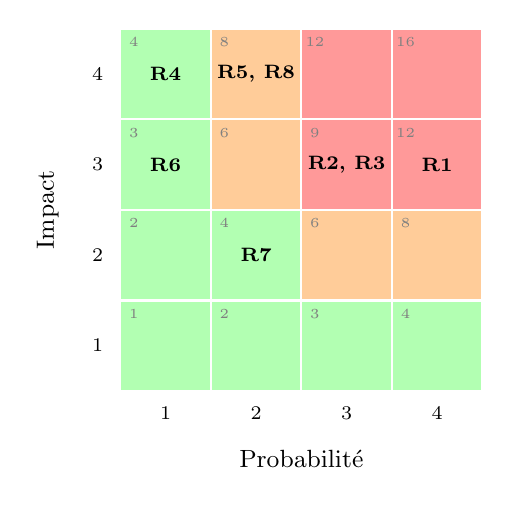
\begin{tikzpicture}[scale=1.15]
\foreach \p in {1,...,4}{
    \foreach \i in {1,...,4}{
        \pgfmathtruncatemacro{\s}{\p*\i}
        \ifnum\s>8 \def\coul{red!40}\else\ifnum\s>4 \def\coul{orange!40}\else\def\coul{green!30}\fi\fi
        \fill[\coul] (\p-1,\i-1) rectangle (\p,\i);
        \draw[white, thick] (\p-1,\i-1) rectangle (\p,\i);
        \node[font=\tiny, color=gray] at (\p-0.85,\i-0.15) {\s};
    }
}
\node[font=\scriptsize\bfseries] at (3.5,2.5) {R1};
\node[font=\scriptsize\bfseries] at (2.5,2.5) {R2, R3};
\node[font=\scriptsize\bfseries] at (1.5,3.5) {R5, R8};
\node[font=\scriptsize\bfseries] at (0.5,3.5) {R4};
\node[font=\scriptsize\bfseries] at (0.5,2.5) {R6};
\node[font=\scriptsize\bfseries] at (1.5,1.5) {R7};
\foreach \k in {1,...,4}{
    \node[font=\scriptsize] at (\k-0.5,-0.25) {\k};
    \node[font=\scriptsize] at (-0.25,\k-0.5) {\k};
}
\node[font=\small] at (2,-0.75) {Probabilité};
\node[font=\small, rotate=90] at (-0.8,2) {Impact};
\end{tikzpicture}
\end{center}
\vspace{-0.4em}
\begin{center}{\small\itshape Figure~5.2. Cartographie des risques
résiduels de LiZbiZ}\end{center}
\end{minipage}

\medskip

La cartographie se lit en trois temps~: les risques en zone rouge sont
traités en priorité~; les risques d'impact~4 restent sous surveillance même
en zone verte, car une erreur sur leur probabilité serait coûteuse~; et
l'écart entre risque inhérent et risque résiduel montre ce que les
contrôles apportent réellement.

\subsection{Quatre options de traitement}

\begin{tableaucours}{L{2.4cm}L{5.0cm}L{4.8cm}}{%
    \tableauHeader{Option} &
    \tableauHeader{Principe} &
    \tableauHeader{Exemple chez LiZbiZ}
}
Réduire & Ajouter ou renforcer des contrôles & Séparer réception et
ajustement (R1) \\
Transférer & Assurance, sous-traitance, sans transférer la responsabilité
& Police d'assurance cyber pour R8 \\
Éviter & Renoncer à l'activité qui crée le risque & Cesser la saisie des
paiements hors application \\
Accepter & Dans les limites de l'appétence, par une décision écrite & R6
résiduel~3, accepté par le comité de direction \\
\end{tableaucours}
\vspace{-0.8em}
\begin{center}{\small\itshape Tableau~5.1. Les options de
traitement}\end{center}

\begin{boxalert}
\textbf{Violation typique.} Considérer qu'un risque confié à un prestataire
« n'est plus le nôtre ».

\smallskip
\textbf{Règle~:} on transfère une conséquence financière (assurance) ou une
exécution (sous-traitance), jamais la responsabilité. Le donneur d'ordre
reste comptable devant ses clients, ses régulateurs et la loi
(Chapitre~\ref{chap:audit-tiers}).
\end{boxalert}

\subsection{Le plan de traitement}

\begin{boxprocedure}
\textbf{Le registre et le plan de traitement.} Pour qu'un auditeur puisse
s'appuyer sur la gestion des risques, chaque risque traité indique~:
\begin{itemize}
    \item le risque, l'objectif menacé et son propriétaire~;
    \item la cotation inhérente, avec la justification de la probabilité et
          de l'impact~;
    \item les contrôles qui le réduisent, avec la date et le résultat de leur
          dernier test~;
    \item la cotation résiduelle et la décision de traitement~;
    \item les actions du plan, leur responsable, leur échéance et leur
          coût~;
    \item la cotation cible attendue après les actions~;
    \item pour un risque accepté, la décision écrite de l'instance
          compétente.
\end{itemize}
\end{boxprocedure}

\begin{tableaucours}{cL{4.2cm}L{2.6cm}L{1.8cm}cc}{%
    \tableauHeader{Réf.} &
    \tableauHeader{Action} &
    \tableauHeader{Responsable} &
    \tableauHeader{Échéance} &
    \tableauHeader{Rés.} & \tableauHeader{Cible}
}
R1 & Retirer F4 aux magasiniers~; validation au-delà de 500~000 & DAF &
30/06/2026 & 12 & 6 \\
R2 & Validation des créations de fournisseurs par le DAF & DAF &
30/06/2026 & 9 & 6 \\
R3 & Procédure de départ, revue trimestrielle des comptes & Resp. RH et
resp. informatique & 31/05/2026 & 9 & 3 \\
R5 & Restauration de test mensuelle & Resp. informatique & 31/07/2026 & 8
& 4 \\
R8 & Sauvegardes hors ligne~; correctifs sous 30 jours & Resp.
informatique & 30/09/2026 & 8 & 4 \\
\end{tableaucours}
\vspace{-0.8em}
\begin{center}{\small\itshape Tableau~5.2. Plan de traitement de LiZbiZ
(extrait)}\end{center}

\subsection{Les indicateurs de risque}

\begin{boxdef}
\termecle{Indicateur clé de risque}\index{indicateur clé de risque}
(\textit{key risk indicator}, KRI)~: mesure régulière qui signale qu'un
risque augmente avant qu'il ne se réalise. Il porte sur une cause ou une
vulnérabilité, pas sur l'incident lui-même.
\end{boxdef}

\begin{tableaucours}{cL{5.2cm}L{3.0cm}L{2.8cm}}{%
    \tableauHeader{Réf.} &
    \tableauHeader{Indicateur} &
    \tableauHeader{Fréquence} &
    \tableauHeader{Seuil d'alerte}
}
R1 & Montant des ajustements négatifs du mois, par entrepôt & Mensuelle &
plus de 10~millions \\
R3 & Comptes actifs d'agents partis depuis plus de 48~h & Hebdomadaire &
plus de 0 \\
R5 & Jours depuis la dernière restauration réussie & Quotidienne & plus de
35 \\
R8 & Serveurs avec un correctif critique de plus de 30~jours &
Hebdomadaire & plus de 0 \\
\end{tableaucours}
\vspace{-0.8em}
\begin{center}{\small\itshape Tableau~5.3. Indicateurs clés de risque de
LiZbiZ}\end{center}

\begin{boxscenario}{Opération SANAGA. Deux registres, deux échelles}
\textbf{Constatation.} La BANQUE SANAGA tient un registre des risques de
crédit et de marché, coté de 1 à 4, et la DSI un registre des risques
informatiques, coté de 1 à 5 avec d'autres critères d'impact.

\medskip
\textbf{Analyse} (confiance élevée). Le conseil ne peut pas comparer un
risque informatique à un risque de crédit, donc ne peut pas arbitrer. La
panne de mars~2026, cotée « 3 sur 5 » par la DSI, n'est jamais apparue
parmi les risques majeurs de la banque. Règle~: le risque informatique est
un risque de l'entreprise, à coter sur l'échelle commune.
\end{boxscenario}

% ============================================================================
\section{La Méthode EBIOS Risk Manager}
\label{sec:c05-ebios}
% ============================================================================

\subsection{Présentation}

EBIOS Risk Manager est la méthode d'appréciation et de traitement des
risques numériques publiée par l'Agence nationale de la sécurité des
systèmes d'information (ANSSI, France) en 2018~\cite{anssi2018ebios}. Elle
part des missions de l'organisation et de ce qu'un attaquant peut viser,
plutôt que d'un inventaire de vulnérabilités. Elle s'organise en cinq
ateliers, et en deux cycles~: un cycle stratégique, revu tous les trois ans
environ, et un cycle opérationnel, revu chaque année.

\begin{tableaucours}{cL{3.4cm}L{4.4cm}L{3.6cm}}{%
    \tableauHeader{N°} &
    \tableauHeader{Atelier} &
    \tableauHeader{Question} &
    \tableauHeader{Produit}
}
1 & Cadrage et socle de sécurité & Que protège-t-on, et à quelles règles
l'organisation est-elle déjà tenue~? & Valeurs métier, biens supports,
événements redoutés, écarts au socle \\
2 & Sources de risque & Qui pourrait attaquer, et dans quel but~? &
Couples source de risque et objectif visé, retenus \\
3 & Scénarios stratégiques & Par quel chemin, à travers l'écosystème~? &
Cartographie des parties prenantes, scénarios stratégiques \\
4 & Scénarios opérationnels & Par quels modes opératoires techniques~? &
Scénarios opérationnels et leur vraisemblance \\
5 & Traitement du risque & Que fait-on, et que reste-t-il~? & Stratégie de
traitement, plan d'amélioration, risques résiduels \\
\end{tableaucours}
\vspace{-0.8em}
\begin{center}{\small\itshape Tableau~5.4. Les cinq ateliers d'EBIOS Risk
Manager}\end{center}

\subsection{Les ateliers appliqués à LiZbiZ}

\begin{boxscenario}{Opération LIZBIZ. Atelier 1, cadrage}
\textbf{Mission retenue.} Livrer et facturer les clients dans les délais.

\textbf{Valeurs métier.} VM1 le suivi des expéditions~; VM2 la facturation~;
VM3 les paiements aux fournisseurs.

\textbf{Biens supports.} L'application intégrée, les quatre centres de
données (Douala, Yaoundé, Garoua, Bafoussam), le réseau entre les sites,
la messagerie.

\textbf{Événements redoutés.} ER1 indisponibilité de la facturation plus de
3~jours (gravité critique)~; ER2 paiements frauduleux (gravité majeure)~;
ER3 divulgation des données clients (gravité majeure, loi n°~2024/017).

\textbf{Socle.} Écarts relevés à la loi n°~2010/012 (sécurité des
systèmes) et à la politique de sécurité interne, inexistante.
\end{boxscenario}

\begin{boxscenario}{Opération LIZBIZ. Atelier 2, sources de risque}
\begin{tableaucours}{L{3.6cm}L{4.4cm}c}{%
    \tableauHeader{Source de risque} &
    \tableauHeader{Objectif visé} &
    \tableauHeader{Retenu}
}
Groupe cybercriminel & Rançon (chiffrement des serveurs) & Oui \\
Salarié ou complice interne & Détournement de fonds par fournisseur fictif
& Oui \\
Ancien salarié & Revente de données clients & Oui \\
Concurrent & Espionnage des tarifs & Non (motivation faible, ressources
faibles) \\
\end{tableaucours}
\end{boxscenario}

\begin{boxscenario}{Opération LIZBIZ. Ateliers 3 et 4, un scénario}
\textbf{Scénario stratégique.} Un groupe cybercriminel compromet le
prestataire de maintenance de Garoua, qui dispose d'un accès distant, puis
chiffre les serveurs de facturation (vise ER1).

\textbf{Scénario opérationnel.} Hameçonnage d'un technicien du prestataire~;
réutilisation de son accès distant sans double authentification~;
élévation de privilèges sur un serveur non corrigé~; désactivation des
sauvegardes accessibles en réseau~; chiffrement.

\textbf{Vraisemblance.} Élevée~: chaque étape repose sur une vulnérabilité
constatée (accès distant à facteur unique, correctifs irréguliers,
sauvegardes en ligne).
\end{boxscenario}

\begin{boxscenario}{Opération LIZBIZ. Atelier 5, traitement}
\textbf{Mesures retenues.} Double authentification pour tout accès
distant~; clause de sécurité et droit d'audit dans le contrat du
prestataire~; correctifs critiques sous 30~jours~; sauvegardes hors ligne
testées chaque mois.

\textbf{Risque résiduel.} ER1 passe de gravité critique et vraisemblance
élevée à gravité critique et vraisemblance faible~: la gravité ne baisse
pas (une indisponibilité reste critique), seule la vraisemblance baisse.
Le risque résiduel est accepté par le comité de direction, avec suivi des
indicateurs R5 et R8 du Tableau~5.3.
\end{boxscenario}

\begin{boxinfo}
\textbf{Ce qu'apporte EBIOS par rapport au registre.} Le registre de
Mme~NKENG cotait R8 (rançongiciel) à partir d'un jugement global. EBIOS
oblige à écrire le chemin d'attaque, étape par étape~; chaque étape est une
hypothèse vérifiable par l'auditeur (l'accès distant est-il à facteur
unique~? les sauvegardes sont-elles en ligne~?). Une cotation devient une
liste de faits à vérifier.
\end{boxinfo}

% ============================================================================
\section{MEHARI et OCTAVE Allegro}
\label{sec:c05-autres}
% ============================================================================

\subsection{MEHARI}

MEHARI (\textit{Méthode harmonisée d'analyse de risques}) est publiée par
le Club de la sécurité de l'information français
(CLUSIF)~\cite{clusif2010mehari}. Elle repose sur des bases de
connaissances~: une liste de scénarios de risque types, et des
questionnaires d'audit des services de sécurité qui mesurent la qualité des
mesures en place. La gravité d'un scénario se déduit de sa potentialité et
de son impact, chacun modulé par la qualité mesurée des services de
sécurité.

\subsection{OCTAVE Allegro}

OCTAVE Allegro est une méthode allégée publiée par le Software Engineering
Institute de l'université Carnegie Mellon~\cite{caralli2007octave}. Elle
est centrée sur les actifs informationnels et leurs « conteneurs »
(techniques, physiques, humains), et conçue pour être menée par une petite
équipe interne en quelques ateliers.

\subsection{Choisir une méthode}

\begin{tableaucours}{L{2.6cm}L{3.6cm}L{3.0cm}L{3.0cm}}{%
    \tableauHeader{Méthode} &
    \tableauHeader{Point de départ} &
    \tableauHeader{Résultat} &
    \tableauHeader{Adaptée à}
}
EBIOS RM & Missions et scénarios d'attaque & Scénarios, plan de traitement
& Organisation exposée à des attaquants ciblés \\
MEHARI & Bases de scénarios et questionnaires & Gravité par scénario,
qualité des mesures & Organisation qui veut un diagnostic complet et
outillé \\
OCTAVE Allegro & Actifs informationnels & Risques par actif & Petite
équipe, première analyse \\
FAIR & Un scénario de perte & Distribution de pertes en valeur & Décision
d'investissement \\
\end{tableaucours}
\vspace{-0.8em}
\begin{center}{\small\itshape Tableau~5.5. Quatre méthodes et leurs
usages}\end{center}

Les méthodes se combinent~: EBIOS ou OCTAVE identifient et structurent les
scénarios, FAIR chiffre ceux qui demandent un arbitrage budgétaire.

% ============================================================================
\section{La Méthode FAIR et la Simulation}
\label{sec:c05-fair}
% ============================================================================

\subsection{La décomposition FAIR}

FAIR (\textit{Factor Analysis of Information Risk}) décompose le risque en
facteurs estimables~\cite{freund2014fair}.

\begin{boxdef}
\termecle{Fréquence des événements de perte}\index{FAIR} (LEF)~: nombre
d'événements de perte par an. $\text{LEF} = \text{TEF} \times V$, où TEF
est la fréquence des tentatives (\textit{threat event frequency}) et $V$ la
vulnérabilité, probabilité qu'une tentative réussisse.

\medskip
\termecle{Ampleur de la perte} (LM)~: perte causée par un événement,
primaire (arrêt, reconstitution, rançon) et secondaire (amendes,
réputation, contentieux).

\medskip
\textbf{Risque}~: distribution de la perte annuelle, résultant de LEF et
LM.
\end{boxdef}

\subsection{Estimer chaque facteur par un intervalle}

\begin{boxscenario}{Opération LIZBIZ. R8 en facteurs}
\textbf{Estimations} (DSI et AUDIX CONSEIL, intervalles à 90~\%, valeur la
plus probable entre parenthèses)~:
\begin{itemize}
    \item TEF~: de 0,5 à 6 tentatives sérieuses par an (2)~;
    \item $V$~: de 2 à 15~\% (5~\%), compte tenu de l'accès distant à
          facteur unique et des correctifs irréguliers~;
    \item LM~: de 100 à 900~millions FCFA par événement (300), arrêt de la
          facturation et reconstitution comprises.
\end{itemize}
\end{boxscenario}

\subsection{Simuler}

Multiplier les valeurs les plus probables ($2 \times 0{,}05 \times 300 =
30$~millions par an) donne un chiffre trompeur~: il ignore l'étendue des
intervalles et l'asymétrie des pertes. La simulation de Monte-Carlo tire
au hasard, des milliers de fois, une valeur de chaque facteur dans sa
distribution, et en déduit la distribution de la perte annuelle.

\begin{boxoutils}{Simulation FAIR en Python}
\begin{lstlisting}[language=Python]
import math, random
random.seed(2026)                   # reproductibilité du résultat
N, pertes = 10_000, []
for _ in range(N):
    tef = random.triangular(0.5, 6.0, 2.0)    # tentatives par an
    v   = random.triangular(0.02, 0.15, 0.05) # succès d'une tentative
    lef = tef * v                             # événements par an
    k, p, seuil = 0, 1.0, math.exp(-lef)      # tirage de Poisson
    while True:
        p *= random.random()
        if p <= seuil: break
        k += 1
    pertes.append(sum(random.triangular(100, 900, 300)
                      for _ in range(k)))     # millions FCFA
pertes.sort()
print(sum(pertes) / N, pertes[N // 2], pertes[int(0.9 * N)])
\end{lstlisting}
\end{boxoutils}

\begin{boxlecture}{Résultat de la simulation de R8}
Sur 10~000~années simulées (graine 2026)~:
\begin{itemize}
    \item perte annuelle moyenne~: environ 87~millions FCFA~;
    \item médiane~: 0 (plus d'une année sur deux sans événement)~;
    \item probabilité d'au moins un événement dans l'année~: 17,6~\%~;
    \item 90\textsuperscript{e} centile~: environ 417~millions~;
          95\textsuperscript{e}~: environ 582~millions~;
    \item probabilité de perdre plus de 500~millions dans l'année~: 7,3~\%.
\end{itemize}

\textbf{Analyse.} La moyenne (87~millions) est presque trois fois le
« calcul rapide » de 30~millions, à cause de l'asymétrie des pertes. Le
conseil peut désormais raisonner en probabilité de dépassement~: une
année sur quatorze environ, LiZbiZ perdrait plus de 500~millions. Avec les
mesures de l'atelier~5 (vulnérabilité ramenée à 1 à 6~\%, perte à 40 à
300~millions), la même simulation donne une moyenne d'environ
12~millions et une probabilité de dépasser 500~millions pratiquement nulle.
\end{boxlecture}

\noindent\begin{minipage}{\linewidth}
\begin{center}
\begin{tikzpicture}
\begin{axis}[width=11cm, height=5.2cm,
    xlabel={Perte annuelle $x$ (millions FCFA)},
    ylabel={$P(\text{perte} > x)$},
    xmin=0, xmax=900, ymin=0, ymax=0.2,
    yticklabel style={/pgf/number format/fixed},
    grid=major, grid style={gray!25}, font=\small]
\addplot[thick, CouleurAccent, mark=*, mark size=1.5pt]
    coordinates {(0,0.176) (200,0.166) (300,0.140) (417,0.100) (500,0.073) (582,0.050) (700,0.029) (900,0.011)};
\end{axis}
\end{tikzpicture}
\end{center}
\vspace{-0.4em}
\begin{center}{\small\itshape Figure~5.3. Courbe de dépassement de R8
(points issus de la simulation)}\end{center}
\end{minipage}

\begin{boxalert}
\textbf{Violation typique.} Présenter le résultat d'une simulation comme une
mesure, sans dire d'où viennent les intervalles.

\smallskip
\textbf{Règle~:} un résultat FAIR vaut ce que valent ses estimations. Le
rapport cite, pour chaque facteur, la source de l'intervalle (données
d'incidents, jugement d'expert calibré) et la graine de la simulation, pour
qu'un tiers puisse la refaire.
\end{boxalert}

% ============================================================================
\section{Auditer la Gestion des Risques}
\label{sec:c05-auditer}
% ============================================================================

L'auditeur n'a pas à refaire l'analyse de risques~: il juge si le dispositif
permet à la direction de connaître et de traiter ses risques.

\begin{boxobjet}{Le registre est justifié}
\textbf{Objectif.} Les priorités de traitement reposent sur des cotations
fondées.

\textbf{Critère.} Chaque risque de score résiduel supérieur ou égal à 9
porte une justification de la probabilité et de l'impact, et renvoie au
rapport de test des contrôles qui le réduisent (procédure de gestion des
risques, ISO~31000 § 6.4).

\textbf{Question.} Les risques intolérables du registre sont-ils justifiés
et leurs contrôles testés~?

\textbf{Risque.} La direction arbitre sur des cotes arbitraires~; un risque
majeur reste sous-estimé.

\textbf{Conséquence.} Ressources mal allouées~; incident non anticipé.

\textbf{Test.} Pour chaque risque intolérable, lecture de la justification
et du rapport de test~; recalcul du résiduel.

\textbf{Preuve et trace.} Copie du registre daté, rapports de test,
feuille de recalcul.
\end{boxobjet}

\begin{boxprocedure}
\textbf{Programme d'audit de la gestion des risques (extrait)}
\begin{enumerate}
    \item Obtenir la procédure, l'échelle, l'appétence approuvée et sa date.
    \item Vérifier que le périmètre couvre les risques informatiques, sur la
          même échelle que les autres risques.
    \item Pour un échantillon de risques, vérifier la justification, le
          propriétaire, le test des contrôles, la décision de traitement.
    \item Vérifier l'avancement du plan de traitement et le suivi des
          indicateurs.
    \item Vérifier qu'un risque accepté l'a été par l'instance compétente,
          par écrit.
    \item Vérifier la mise à jour après les incidents majeurs de la période.
\end{enumerate}
\end{boxprocedure}

\begin{boxmetier}{Gestionnaire de risques}
\textbf{Tenir une cartographie utile}
\begin{enumerate}
    \item Faire approuver l'échelle de cotation et l'appétence par le
          conseil, avant toute cotation.
    \item Désigner un propriétaire par risque, au niveau de la direction.
    \item Ne réduire le risque résiduel que sur la base de contrôles testés.
    \item Mettre à jour la cartographie au moins une fois par an, et après
          tout incident majeur.
    \item Présenter au comité d'audit les risques en zone rouge et les
          décisions d'acceptation.
\end{enumerate}
\end{boxmetier}

\begin{boxmetier}{RSSI}
\textbf{Alimenter EBIOS avec des faits.} Le RSSI fournit à chaque atelier
les éléments vérifiables~: état des correctifs, liste des accès distants,
résultat des tests de sauvegarde. Un scénario opérationnel qui repose sur
une hypothèse non vérifiée est marqué comme tel.
\end{boxmetier}

\begin{boxinfo}
\textbf{Ce que dit la recherche.} Une méthode d'analyse de risques produit
des cotes~; l'auditologie~\cite{minka2026auditologie} demande en plus ce que
l'on sait de chaque cote. Les intervalles de FAIR et les écarts entre
évaluateurs (Chapitre~\ref{chap:risque}) sont deux façons de rendre cette
connaissance visible, que la lecture $\mu$, $U$, $H$ rend comparable d'un
domaine à l'autre.
\end{boxinfo}

\separateur

\begin{boxresume}
\textbf{Ce qu'il faut retenir de ce chapitre~:}
\begin{itemize}
    \item \textbf{Le processus ISO~31000}~: contexte, appréciation
          (identifier, analyser, évaluer), traitement, surveillance, avec
          communication et enregistrement à chaque étape~; l'ISO/IEC~27005
          l'applique à la sécurité de l'information.
    \item \textbf{La cartographie} montre les priorités~; le plan de
          traitement les transforme en actions datées et chiffrées~; les
          indicateurs clés signalent un risque qui monte.
    \item \textbf{Quatre options}~: réduire, transférer, éviter, accepter~;
          la responsabilité ne se transfère pas.
    \item \textbf{EBIOS Risk Manager}~: cinq ateliers, du cadrage au
          traitement, qui transforment une cote en chemin d'attaque
          vérifiable.
    \item \textbf{MEHARI} et \textbf{OCTAVE Allegro} offrent un diagnostic
          outillé ou allégé~; \textbf{FAIR} chiffre un scénario en
          distribution de pertes par simulation.
    \item \textbf{Auditer la gestion des risques}, c'est vérifier les
          justifications, les tests, les décisions et le suivi, pas refaire
          l'analyse.
\end{itemize}
\end{boxresume}

\begin{boxinfo}
\textbf{Points de contrôle de l'élève.} Je sais~: dessiner le processus
ISO~31000~; nommer les cinq ateliers d'EBIOS~; écrire un indicateur clé de
risque~; décomposer un risque en facteurs FAIR~; lire une courbe de
dépassement~; rédiger trois étapes d'un programme d'audit de la gestion des
risques.
\end{boxinfo}

\bigskip

\begin{boxexo}[title={\ding{45}\quad Exercice~5.1. Le processus \niveaubase}]
Pour chacune des activités suivantes, indiquez l'étape du processus
ISO~31000 à laquelle elle appartient~: (a) le conseil fixe l'appétence~;
(b) trois responsables cotent R8~; (c) on compare R1 au seuil de 9~; (d) on
retire le droit F4 aux magasiniers~; (e) on suit chaque mois le montant des
ajustements négatifs.
\end{boxexo}

\begin{boxexo}[title={\ding{45}\quad Exercice~5.2. Choisir une option \niveaubase}]
Proposez une option de traitement, justifiée, pour R4, R6 et R7 du registre
de LiZbiZ.
\end{boxexo}

\begin{boxexo}[title={\ding{45}\quad Exercice~5.3. Des indicateurs \niveaumoyen}]
Proposez un indicateur clé de risque, sa fréquence et son seuil d'alerte
pour R2 et R6. Expliquez pourquoi « nombre d'incidents de fraude » n'est pas
un bon indicateur clé de risque.
\end{boxexo}

\begin{boxexo}[title={\ding{45}\quad Exercice~5.4. Atelier 2 d'EBIOS \niveaumoyen}]
Pour la BANQUE SANAGA, proposez quatre couples source de risque et
objectif visé, et dites lesquels vous retenez, en justifiant par la
motivation et les ressources de la source.
\end{boxexo}

\begin{boxexo}[title={\ding{45}\quad Exercice~5.5. Un scénario opérationnel \niveaumoyen}]
Rédigez, pour l'événement redouté ER2 de LiZbiZ (paiements frauduleux), un
scénario stratégique et le scénario opérationnel correspondant, en quatre
étapes. Pour chaque étape, indiquez le fait que l'auditeur devrait vérifier.
\end{boxexo}

\begin{boxexo}[title={\ding{45}\quad Exercice~5.6. Le calcul rapide \niveaumoyen}]
Expliquez pourquoi le produit des valeurs les plus probables
($2 \times 0{,}05 \times 300$) sous-estime la perte moyenne de R8. Calculez
la moyenne de chaque loi triangulaire (la moyenne de la loi triangulaire
de paramètres $a$, $b$, $c$ vaut $(a+b+c)/3$) et vérifiez que leur produit
est proche du résultat de la simulation.
\end{boxexo}

\begin{boxexo}[title={\ding{45}\quad Exercice~5.7. Lire une distribution \niveaumoyen}]
Le conseil de LiZbiZ envisage une assurance cyber qui couvre les pertes
au-delà de 200~millions par an, plafonnées à 1~milliard, pour une prime de
25~millions. À partir du résultat de la simulation, quelles informations
supplémentaires demandez-vous pour conseiller le conseil~? Quelle donnée
de la simulation est la plus utile ici~?
\end{boxexo}

\begin{boxexo}[title={\ding{45}\quad Exercice~5.8. Auditer un registre \niveaumoyen}]
Le registre de la BANQUE SANAGA contient 64~risques, dont 9 informatiques.
Rédigez une fiche d'assertion pour le contrôle « les risques informatiques
sont cotés sur l'échelle commune de la banque », puis cotez-la à partir de
la constatation du scénario « Deux registres, deux échelles ».
\end{boxexo}

\begin{boxexo}[title={\ding{45}\quad Exercice~5.9. Choisir une méthode \niveauexpert}]
L'agence publique ANPP veut analyser les risques de sa nouvelle plateforme
de paie, avec une équipe de trois personnes et sans budget de conseil. Le
ministère des Finances exige un chiffrage des pertes possibles avant de
financer un site de secours. Quelle combinaison de méthodes recommandez-
vous, et dans quel ordre~? Justifiez.
\end{boxexo}

\begin{boxexo}[title={\ding{45}\quad Exercice~5.10. Simulation et décision \niveauexpert}]
Modifiez la simulation de la section~\ref{sec:c05-fair} pour comparer deux
mesures~: (A) double authentification des accès distants, qui ramène $V$ à
1 à 6~\% (2~\%)~; (B) sauvegardes hors ligne testées, qui ramènent la perte
par événement à 40 à 300~millions (100). Écrivez le code, décrivez le
résultat attendu (sans l'exécuter, en raisonnant sur les moyennes), et
dites quelle mesure vous recommanderiez si une seule était finançable.
\end{boxexo}

\bigskip

\begin{boxinfo}
\textbf{Pour aller plus loin.}
\begin{itemize}
    \item ANSSI, \textit{EBIOS Risk Manager. Le guide}~\cite{anssi2018ebios}~:
          la méthode complète, avec un cas d'étude.
    \item J.~Freund et J.~Jones, \textit{Measuring and Managing
          Information Risk: A FAIR Approach}~\cite{freund2014fair}~: la
          référence de la méthode FAIR.
    \item ISO/IEC~27005:2022~\cite{iso27005_2022}~: le processus appliqué à
          la sécurité de l'information.
    \item R.~Caralli et al., \textit{Introducing OCTAVE
          Allegro}~\cite{caralli2007octave}~: une méthode légère, avec ses
          fiches de travail.
\end{itemize}
\end{boxinfo}

\begin{boxinfo}
\textbf{Transition.} Trois des risques intolérables de LiZbiZ supposent une
intention~: ajuster le stock, payer des fournisseurs fictifs, utiliser le
compte d'un agent parti. Le Chapitre~\ref{chap:fraude} est consacré à la
fraude dans et par les systèmes d'information.
\end{boxinfo}
}{}
        \IfFileExists{partie1/P01_C06_fraude.tex}{% ============================================================================
% Fichier  : partie1/P01_C06_fraude.tex
% Titre    : La Fraude dans et par les Systèmes d'Information
% Auteur   : MINKA MI NGUIDJOÏ Thierry Emmanuel
% Version  : 1.0 -- novembre 2026
% ============================================================================
% Base : ACSI C04 (TRANSLOG SERVICES 23 × 4,9 M = 112,7 M ; ajustements de
% FOUDA 148 M dont 71 % le dernier jour ouvré ; 38 M de l'écart de 186 M
% cotés NEK ; Douala 17/2/1 puis 9/3/8).
% Sources : COSO et ACFE, guide de gestion du risque de fraude (2016) ;
% Cressey (1953) ; Wolfe et Hermanson (2004), losange de la fraude ;
% Benford (1938) et Nigrini (2012) pour la loi du premier chiffre ; COSO
% 2013 (principe 8) ; A0 (axiome 4), A1 (usage stratégique de NEK).
% Données Benford : fichier paiements_fournisseurs_2025.csv du lab
% ACSI-LAB-07 (4 812 paiements) ; calcul du 06/11/2026 : premier chiffre,
% khi-deux 10,4, MAD 0,0035 ; deux premiers chiffres « 49 » : 60 observés
% pour 42,2 attendus.
% L'obligation de révélation du commissaire aux comptes (AUSCGIE) est
% décrite sans numéro d'article : à vérifier dans le texte.
% Corrigés : corriges/Corr_C06.tex.
% ============================================================================

\chapter{La Fraude dans et par les Systèmes d'Information}
\label{chap:fraude}
\chaptermark{La fraude et les SI}

\epigraph{%
    « L'erreur se cache par hasard.\\
    La fraude se cache exprès~: c'est ce qui la rend auditable. »%
}{Principe de l'auditeur}

\niveauChapitre{Intermédiaire}{%
    Maîtrise des Chapitres~\ref{chap:controle-interne} (séparation des
    tâches), \ref{chap:risque} et~\ref{chap:gestion-risques} (risque,
    registre, scénarios)%
}

\begin{boxobjectifs}
\begin{itemize}
    \item Définir la fraude, la distinguer de l'erreur, et en classer les
          formes.
    \item Expliquer le triangle et le losange de la fraude, et les relier à
          l'interaction stratégique entre auditeur et audité.
    \item Classer les schémas de fraude assistés par l'informatique et
          leurs signaux dans les données.
    \item Écrire les requêtes de détection des principaux schémas et
          appliquer la loi de Benford, en connaissant ses limites.
    \item Concevoir un dispositif de gestion du risque de fraude selon le
          guide du COSO et de l'ACFE.
    \item Reconnaître un usage stratégique de la réponse \NEK{}.
    \item Savoir quand l'audit doit s'arrêter et laisser place à
          l'enquête.
\end{itemize}
\end{boxobjectifs}

\bigskip

% ============================================================================
\section*{Question directrice : erreur ou fraude~?}
% ============================================================================

Au Chapitre~\ref{chap:risque}, trois risques intolérables de LiZbiZ
supposaient une intention~: ajuster le stock, payer des fournisseurs
fictifs, utiliser le compte d'un agent parti. Lorsque AUDIX CONSEIL
présente sa cartographie, le responsable informatique proteste~: « Ce sont
des erreurs de saisie, pas des fraudes. Nos agents sont honnêtes. »

Peut-être. Mais l'auditeur ne présume ni l'honnêteté ni la malhonnêteté~: il
cherche des faits. Et il sait qu'une fraude ne se trouve pas par hasard~:
elle se trouve parce qu'on connaît ses schémas et qu'on sait où regarder.

\medskip
\textbf{Plan du chapitre.}
\begin{enumerate}
    \item Définir et classer la fraude (section~\ref{sec:c06-definir}).
    \item Pourquoi elle survient (section~\ref{sec:c06-triangle}).
    \item Ses schémas dans les SI (section~\ref{sec:c06-schemas}).
    \item Le dispositif anti-fraude (section~\ref{sec:c06-dispositif}).
    \item La repérer dans les données, par requêtes et par la loi de
          Benford (sections~\ref{sec:c06-donnees} et~\ref{sec:c06-benford}).
    \item La repérer dans les réponses (section~\ref{sec:c06-strategie}).
    \item De l'audit à l'enquête (section~\ref{sec:c06-enquete}).
\end{enumerate}

\separateur

% ============================================================================
\section{Définir la Fraude}
\label{sec:c06-definir}
% ============================================================================

\begin{boxdef}
\termecle{Fraude}\index{fraude}~: acte \emph{intentionnel}, commis par une ou
plusieurs personnes de l'organisation ou extérieures à elle, qui recourt à
la tromperie pour obtenir un avantage indu ou causer un préjudice.

\medskip
\termecle{Erreur}\index{erreur}~: inexactitude \emph{non intentionnelle}
(faute de saisie, mauvaise interprétation d'une règle, panne).
\end{boxdef}

Ce qui distingue la fraude de l'erreur, c'est l'intention, et donc la
\emph{dissimulation}. Une erreur laisse des traces au hasard~; une fraude
efface les siennes, ou les place là où personne ne regarde. C'est pourquoi
la fraude obéit à des schémas, que l'auditeur peut connaître.

\begin{tableaucours}{L{3.6cm}L{4.4cm}L{4.2cm}}{%
    \tableauHeader{Famille} &
    \tableauHeader{Définition} &
    \tableauHeader{Exemple chez LiZbiZ}
}
Détournement d'actifs & Appropriation de biens ou de fonds de
l'organisation & Vol de marchandises masqué par un ajustement de stock \\
Corruption & Usage de sa fonction pour obtenir un avantage indu, souvent
avec un tiers & Commission versée par un transporteur pour être
retenu \\
Fraude à l'information financière & Présentation trompeuse des états
financiers & Stock surévalué pour améliorer le résultat \\
\end{tableaucours}
\vspace{-0.8em}
\begin{center}{\small\itshape Tableau~6.1. Trois familles de fraude
(classification usuelle de la profession)}\end{center}

\subsection{Fraude interne, fraude externe, fraude par le système}

Une deuxième classification croise l'auteur et le rôle du système.

\begin{tableaucours}{L{3.0cm}L{4.6cm}L{4.6cm}}{%
    \tableauHeader{} &
    \tableauHeader{Auteur interne} &
    \tableauHeader{Auteur externe}
}
Fraude \emph{dans} le système (le SI enregistre une opération frauduleuse)
& Fournisseur fictif, ajustement de stock & Faux client, fausse facture
d'un fournisseur réel \\
Fraude \emph{par} le système (le SI est l'arme) & Abus d'administrateur,
modification d'un paramètre & Hameçonnage, usurpation du dirigeant,
rançongiciel \\
\end{tableaucours}
\vspace{-0.8em}
\begin{center}{\small\itshape Tableau~6.2. Fraude dans et par le
système}\end{center}

\begin{boxinfo}
\textbf{L'usurpation du dirigeant.} Un comptable reçoit un courriel ou un
appel, apparemment du directeur général, qui demande un virement urgent et
confidentiel vers un compte à l'étranger. C'est une fraude externe par le
système~: aucune règle de l'application n'est violée, le paiement est
« normalement » saisi et validé. Le contrôle est procédural (rappel par un
numéro connu, double validation de tout nouveau bénéficiaire), pas
technique.
\end{boxinfo}

% ============================================================================
\section{Pourquoi la Fraude Survient}
\label{sec:c06-triangle}
% ============================================================================

\subsection{Le triangle de la fraude}

Dans les années 1950, le criminologue Donald Cressey étudie des personnes
condamnées pour détournement de fonds~\cite{cressey1953}. Ses travaux ont
donné naissance au \termecle{triangle de la fraude}\index{triangle de la
fraude}~: la fraude survient lorsque trois conditions sont réunies.

\noindent\begin{minipage}{\linewidth}
\begin{center}
\begin{tikzpicture}[
    sommet/.style = {
        draw=CouleurPrimaire, fill=CouleurDef, rounded corners=4pt,
        text width=3.2cm, align=center, minimum height=1.0cm,
        font=\small\bfseries\color{CouleurPrimaire}
    }
]
\coordinate (A) at (0,3.0);
\coordinate (B) at (-3.0,0);
\coordinate (C) at (3.0,0);
\draw[very thick, color=CouleurAccent] (A) -- (B) -- (C) -- cycle;
\node[sommet] at (A) {Pression\\ \mdseries\footnotesize dette, objectifs intenables};
\node[sommet] at (B) {Opportunité\\ \mdseries\footnotesize contrôle faible, droits cumulés};
\node[sommet] at (C) {Rationalisation\\ \mdseries\footnotesize « je le rendrai », « on me doit »};
\node[font=\footnotesize\itshape, color=CouleurSecondaire] at (0,1.0) {Fraude};
\end{tikzpicture}
\end{center}
\vspace{-0.4em}
\begin{center}{\small\itshape Figure~6.1. Le triangle de la fraude, d'après
les travaux de Cressey}\end{center}
\end{minipage}

\medskip

L'auditeur et le contrôleur interne n'ont guère de prise sur la pression ni
sur la rationalisation. Ils agissent sur l'\textbf{opportunité}~: c'est
pourquoi la séparation des tâches et la revue des droits
(Chapitre~\ref{chap:controle-interne}) sont les premières défenses contre la
fraude.

\subsection{Le losange~: la capacité}

D.~Wolfe et D.~Hermanson ont ajouté en 2004 un quatrième élément, la
\termecle{capacité}\index{losange de la fraude}~: la position, les
compétences et l'assurance qui permettent de passer à l'acte et de
dissimuler~\cite{wolfe2004diamond}. Dans les systèmes d'information, cette
capacité est souvent technique~: un administrateur peut faire ce que le
contrôle interne interdit aux autres, et effacer la trace de ce qu'il a
fait. C'est la raison pour laquelle le cumul total de M.~KOUNOU
(Chapitre~\ref{chap:controle-interne}) est le plus grave~: il réunit
l'opportunité et la capacité.

\subsection{Un jeu entre l'auditeur et l'audité}

L'auditologie pose que l'auditeur et l'audité poursuivent des intérêts
distincts, et que leurs actions se comprennent comme des coups dans un jeu
à information imparfaite (axiome~4~\cite{minka2026auditologie}). La fraude en
est le cas extrême~: le fraudeur sait ce que l'auditeur ignore, et cherche à
ce qu'il continue de l'ignorer. Deux conséquences pratiques en découlent.
\begin{enumerate}
    \item \textbf{L'audité adapte ses réponses à l'enjeu.} Une même personne
          ne répond pas de la même façon dans une auto-évaluation et dans un
          entretien formel (section~\ref{sec:c06-strategie}).
    \item \textbf{L'auditeur doit être imprévisible.} Un programme de tests
          connu d'avance indique au fraudeur où ne pas laisser de traces~:
          les échantillons, les dates et certains tests doivent rester
          inconnus de l'audité.
\end{enumerate}

% ============================================================================
\section{Les Schémas de Fraude Assistés par l'Informatique}
\label{sec:c06-schemas}
% ============================================================================

\begin{tableaucours}{L{2.9cm}L{3.2cm}L{3.0cm}L{3.1cm}}{%
    \tableauHeader{Schéma} &
    \tableauHeader{Vulnérabilité exploitée} &
    \tableauHeader{Contrôle préventif} &
    \tableauHeader{Signal dans les données}
}
Fournisseur fictif & Cumul création du fournisseur et paiement & Séparation
des tâches, validation des nouveaux fournisseurs & Coordonnées bancaires
partagées avec un salarié, absence d'adresse \\
Modification des coordonnées bancaires & Données de référence modifiables
sans validation & Double validation, journal des modifications &
Changement de RIB suivi d'un paiement dans les jours suivants \\
Fausse réception & Cumul commande et réception & Réception confirmée par
une personne distincte & Réception sans bon de transport, à l'heure de
fermeture \\
Ajustement de stock & Cumul réception et ajustement & Validation au-delà
d'un seuil & Ajustements concentrés en fin de mois, sans pièce \\
Fractionnement & Seuil de validation connu & Contrôle des cumuls par
fournisseur & Paiements juste sous le seuil, répétés \\
Compte dormant & Comptes d'agents partis non désactivés & Revue périodique
des comptes & Connexion après la date de départ \\
Abus d'administrateur & Droits techniques étendus, sans trace & Comptes
nominatifs, journalisation protégée & Opérations de gestion faites par un
compte d'administration \\
Salarié fantôme & Fichier de paie modifiable sans contrôle & Rapprochement
paie et effectif des services & Même RIB pour deux salariés, absence de
congés \\
\end{tableaucours}
\vspace{-0.8em}
\begin{center}{\small\itshape Tableau~6.3. Schémas de fraude et
signaux}\end{center}

\begin{boxalert}
\textbf{Violation typique.} Laisser le responsable informatique, qui détient
tous les droits, administrer lui-même les journaux qui tracent ses propres
actions.

\smallskip
\textbf{Règle~:} les journaux des comptes d'administration sont conservés
hors de leur portée et examinés par une personne indépendante.
\end{boxalert}

% ============================================================================
\section{Le Dispositif Anti-Fraude}
\label{sec:c06-dispositif}
% ============================================================================

Le principe~8 du COSO~2013 demande de prendre en compte le risque de fraude
(Chapitre~\ref{chap:controle-interne}). Le COSO et l'Association of
Certified Fraud Examiners (\sigle{ACFE}) ont publié en 2016 un guide qui
décline cette exigence en un programme global de gestion du risque de
fraude~\cite{coso2016fraude}. Ses cinq principes sont alignés sur les cinq
composantes du contrôle interne.

\begin{tableaucours}{L{3.6cm}L{8.6cm}}{%
    \tableauHeader{Volet} &
    \tableauHeader{Contenu (reformulé)}
}
Gouvernance & Une politique écrite de gestion du risque de fraude, portée
par l'organe de gouvernance et la direction \\
Évaluation & Une évaluation régulière et complète du risque de fraude,
schéma par schéma \\
Activités de contrôle & Des contrôles préventifs et détectifs choisis pour
les schémas identifiés \\
Investigation et correction & Un dispositif de signalement et une approche
coordonnée des investigations et des mesures correctives \\
Pilotage & Des évaluations qui vérifient que les cinq volets fonctionnent,
et la communication des déficiences \\
\end{tableaucours}
\vspace{-0.8em}
\begin{center}{\small\itshape Tableau~6.4. Les cinq volets de la gestion du
risque de fraude (d'après COSO et ACFE, 2016)}\end{center}

\begin{boxmetier}{Contrôleur interne}
\textbf{Bâtir le programme anti-fraude de LiZbiZ}
\begin{enumerate}
    \item Faire adopter par le conseil une politique anti-fraude~: tolérance
          zéro, obligation de signaler, protection des lanceurs d'alerte.
    \item Dresser, schéma par schéma, la liste des fraudes possibles dans
          l'application intégrée (Tableau~6.3).
    \item Supprimer d'abord les opportunités~: cumuls de droits, comptes
          dormants, seuils connus et non surveillés.
    \item Mettre en place des contrôles détectifs automatiques sur les
          données, revus chaque mois.
    \item Ouvrir un canal de signalement confidentiel, hors de la
          hiérarchie directe.
\end{enumerate}
\end{boxmetier}

% ============================================================================
\section{Repérer la Fraude dans les Données}
\label{sec:c06-donnees}
% ============================================================================

\subsection{Analyser toute la population}

L'informatique facilite la fraude, mais elle en garde la trace. L'auditeur
analyse l'ensemble des opérations, et non un échantillon, à la recherche des
signaux du Tableau~6.3~: doublons, valeurs juste sous un seuil, opérations
hors des heures de travail, coordonnées partagées entre un fournisseur et un
salarié.

\begin{boxoutils}{Trois requêtes de détection}
\begin{lstlisting}[language=SQL]
-- 1. Paiements juste sous le seuil de double validation (5 M)
SELECT id_fournisseur, COUNT(*) AS nb, SUM(montant_fcfa) AS total
FROM   paiements
WHERE  montant_fcfa >= 4500000 AND montant_fcfa < 5000000
GROUP  BY id_fournisseur
HAVING COUNT(*) >= 3
ORDER  BY total DESC;

-- 2. Fournisseurs dont le RIB est celui d'un salarié
SELECT f.id_fournisseur, f.nom, s.matricule
FROM   fournisseurs f
JOIN   salaries s ON REPLACE(f.rib, ' ', '') = REPLACE(s.rib, ' ', '');

-- 3. Ajustements négatifs du dernier jour ouvré, par magasinier
SELECT saisi_par, SUM(-quantite * prix_unitaire) AS valeur
FROM   ajustements a
JOIN   calendrier c ON c.jour = a.date_ajustement
WHERE  a.quantite < 0 AND c.dernier_ouvre_du_mois = 1
GROUP  BY saisi_par;
\end{lstlisting}
\end{boxoutils}

\begin{boxscenario}{Opération LIZBIZ. Ce que disent les données}
\textbf{Tests réalisés} par AUDIX CONSEIL sur les extractions de l'application
intégrée, pour 2025 et le premier trimestre~2026.

\medskip
\textbf{Constatation 1.} Le fournisseur « TRANSLOG SERVICES », créé en
mars~2025 par Mme~OWONA, a reçu 23~paiements de 4,9~millions FCFA chacun,
soit 112,7~millions FCFA. Le seuil de double validation est de 5~millions.
Ses coordonnées bancaires sont identiques à celles qu'un salarié a déclarées
pour sa paie.

\medskip
\textbf{Constatation 2.} À l'entrepôt de Douala, les ajustements négatifs de
stock saisis par M.~FOUDA s'élèvent à 148~millions FCFA, dont 71~\% le
dernier jour ouvré du mois. Aucun n'est appuyé par un procès-verbal
d'inventaire.

\medskip
\textbf{Constatation 3.} Sur l'écart de stock de 186~millions FCFA, 38~millions
ne peuvent être rattachés à aucune opération~: les extractions des autres
entrepôts sont incomplètes.

\medskip
\textbf{Analyse} (confiance moyenne). Les constatations 1 et 2 réunissent
les signaux de deux schémas~: fournisseur fictif avec fractionnement, et
ajustement de stock. Elles ne prouvent pas une fraude, car l'intention reste
à établir, mais elles imposent d'en informer le commanditaire. La
constatation 3 est cotée \NEK{}~: on ne sait pas, et il faut dire pourquoi.
\end{boxscenario}

\begin{boxalert}
\textbf{Violation typique.} Écrire dans le rapport « Mme~OWONA a détourné
112,7~millions ».

\smallskip
\textbf{Règle~:} l'auditeur constate des faits («~23~paiements de
4,9~millions à un fournisseur créé par Mme~OWONA, dont le RIB est celui
d'un salarié~») et s'abstient de toute qualification pénale. Qualifier,
c'est le rôle du juge~; accuser sans preuve de l'intention expose
l'auditeur et sa mission.
\end{boxalert}

% ============================================================================
\section{La Loi de Benford}
\label{sec:c06-benford}
% ============================================================================

\subsection{Le premier chiffre n'est pas uniforme}

Dans de nombreuses séries de montants naturels (factures, paiements,
populations), le premier chiffre significatif n'est pas réparti au hasard
entre 1 et 9~: il vaut 1 dans environ 30~\% des cas, et 9 dans moins de
5~\%. Cette régularité, observée par Frank Benford en
1938~\cite{benford1938}, suit la loi
\[
    P(d) = \log_{10}\!\left(1 + \frac{1}{d}\right), \qquad d = 1, \dots, 9.
\]
Elle s'étend aux deux premiers chiffres~: $P(d_1d_2) =
\log_{10}(1 + 1/d_1d_2)$, pour $d_1d_2$ de 10 à 99. M.~Nigrini a fait de
ces tests un outil de l'audit et de la détection de
fraude~\cite{nigrini2012benford}.

\subsection{Les paiements de LiZbiZ}

\begin{boxscenario}{Opération LIZBIZ. Le test du premier chiffre}
\textbf{Données.} Les 4~812~paiements fournisseurs de 2025 (fichier
\texttt{paiements\_fournisseurs\_2025.csv}).

\medskip
\begin{tableaucours}{cccc}{%
    \tableauHeader{Chiffre} & \tableauHeader{Observés} &
    \tableauHeader{Part observée} & \tableauHeader{Part attendue}
}
1 & 1~443 & 30,0~\% & 30,1~\% \\
2 & 813 & 16,9~\% & 17,6~\% \\
3 & 574 & 11,9~\% & 12,5~\% \\
4 & 461 & 9,6~\% & 9,7~\% \\
5 & 378 & 7,9~\% & 7,9~\% \\
6 & 332 & 6,9~\% & 6,7~\% \\
7 & 292 & 6,1~\% & 5,8~\% \\
8 & 284 & 5,9~\% & 5,1~\% \\
9 & 235 & 4,9~\% & 4,6~\% \\
\end{tableaucours}

\medskip
\textbf{Constatation.} Khi-deux à 8~degrés de liberté~: 10,4, inférieur à
la valeur critique de 15,5 au seuil de 5~\%~; écart absolu moyen (MAD)~:
0,0035. La distribution est conforme à la loi de Benford.

\medskip
\textbf{Test des deux premiers chiffres.} Les montants commençant par
« 49 » sont 60, pour 42,2 attendus. L'écart réduit vaut environ
$(60 - 42{,}2)/\sqrt{42{,}2} \approx 2{,}7$~: il est significatif, alors que
la distribution globale reste conforme.

\medskip
\textbf{Analyse.} Le test du premier chiffre ne voit pas les 23~paiements de
TRANSLOG SERVICES, noyés dans 4~812 opérations. Le test des deux premiers
chiffres les fait apparaître~: il est plus fin, et c'est lui qui oriente
vers la requête des paiements juste sous le seuil.
\end{boxscenario}

\begin{boxalert}
\textbf{Violation typique.} Conclure « pas de fraude » parce que la
distribution du premier chiffre est conforme à la loi de Benford, ou
« fraude » parce qu'elle ne l'est pas.

\smallskip
\textbf{Règle~:} la loi de Benford oriente, elle ne prouve rien. Elle ne
s'applique pas aux montants fixés (loyers, salaires, tarifs), bornés ou
attribués (numéros). Un écart désigne où regarder~; une conformité ne
rassure que sur l'ensemble, jamais sur une sous-population.
\end{boxalert}

% ============================================================================
\section{Repérer la Dissimulation dans les Réponses}
\label{sec:c06-strategie}
% ============================================================================

Le prologue l'a annoncé~: les réponses données en entretien formel ont
différé de celles de l'auto-évaluation. La réponse \NEK{} peut traduire une
ignorance sincère~; elle peut aussi servir à ne pas répondre. L'article
\emph{Modelling Epistemic Uncertainty in IS Audit} propose un indice, le
\termecle{SUI}\index{SUI (indice d'usage stratégique)} (\textit{Strategic Use
Index}), qui compare la distribution des \NEK{} entre questions à fort enjeu
et à faible enjeu, pour distinguer l'ignorance authentique de la
dissimulation~\cite{minka2026nek}. Le Chapitre~\ref{chap:incertitude} en
donnera la définition.

\begin{boxlecture}{Entrepôt de Douala}
Les mêmes dix questions sur la gestion du stock de Douala sont posées aux
mêmes deux responsables, d'abord en auto-évaluation écrite, puis en
entretien formel, après la découverte des ajustements.

\medskip
\begin{tableaucours}{L{3.6cm}ccccc}{%
    \tableauHeader{Contexte} &
    \tableauHeader{\OUI{}} & \tableauHeader{\NON{}} & \tableauHeader{\NEK{}} &
    \tableauHeader{$U$} & \tableauHeader{$H$ (bit)}
}
Auto-évaluation & 17 & 2 & 1 & 0,05 & 0,75 \\
Entretien formel & 9 & 3 & 8 & 0,40 & 1,46 \\
\end{tableaucours}

\medskip
\textbf{Constatation.} Le taux de \NEK{} passe de 5~\% à 40~\% lorsque
l'enjeu augmente, pour les mêmes personnes et les mêmes questions.

\medskip
\textbf{Analyse} (confiance faible à moyenne). Une ignorance sincère ne
devrait pas dépendre du contexte. Ce déplacement est un \emph{signal}
d'usage stratégique de \NEK{}, pas une preuve~: d'autres explications sont
possibles, comme la crainte de se tromper devant un auditeur. Il oriente
les tests vers les questions où \NEK{} a le plus augmenté.

\medskip
\hfill\lecture{0{,}45}{0{,}40}{1{,}46}
\end{boxlecture}

% ============================================================================
\section{De l'Audit à l'Enquête}
\label{sec:c06-enquete}
% ============================================================================

L'auditeur n'est ni un enquêteur ni un juge. Lorsque ses travaux révèlent des
indices sérieux de fraude, il ne poursuit pas seul.

\begin{boxprocedure}
\textbf{Conduite à tenir devant des indices de fraude.} Le papier de travail
de l'auditeur doit permettre d'établir qu'il a~:
\begin{itemize}
    \item conservé les extractions et les journaux utilisés, avec leur
          empreinte numérique, sans les modifier~;
    \item consigné les constatations séparément de leur analyse, sans
          qualification pénale («~fraude~», «~vol~»)~;
    \item informé le commanditaire désigné par la lettre de mission, par
          écrit, et non les personnes mises en cause~;
    \item suspendu les tests susceptibles d'alerter les personnes en cause,
          dans l'attente de la décision du commanditaire.
\end{itemize}
\end{boxprocedure}

La suite relève d'une enquête interne, d'un expert judiciaire ou de la
justice. Elle obéit aux règles de la preuve numérique~: chaîne de
conservation, intégrité, opposabilité. Le Chapitre~\ref{chap:audit-preuve}
et les cours d'investigation numérique (UE~SEC4031 et SEC4052) y reviennent.

\begin{boxinfo}
\textbf{Le commissaire aux comptes.} Informé des constatations d'AUDIX
CONSEIL, le commissaire aux comptes de LiZbiZ doit en apprécier l'effet sur
les comptes~: stock surévalué, charges fictives. Le droit OHADA des
sociétés commerciales lui impose en outre de révéler au ministère public
les faits délictueux dont il a connaissance dans l'exercice de sa
mission~\cite{ohada2014auscgie} (l'article est à vérifier dans le texte
avant toute citation). Il ne peut donc pas «~régler l'affaire en interne~».
\end{boxinfo}

\begin{boxmetier}{Responsable de la conformité}
\textbf{Protéger le canal de signalement.} Le responsable de la conformité
s'assure que les signalements reçus sont enregistrés, traités par une
personne indépendante des personnes mises en cause, et que leur auteur
n'est pas exposé. Un canal que personne n'ose utiliser ne détecte rien.
\end{boxmetier}

\begin{boxmetier}{Auditeur SI}
\textbf{Fournir des preuves exploitables.} Devant des indices, l'auditeur
SI remet au commanditaire les requêtes exécutées, les extractions et leurs
empreintes SHA-256, et la lettre d'extraction qui atteste leur origine.
Une enquête qui doit tout refaire perd des semaines, et parfois la preuve.
\end{boxmetier}

\begin{boiteRemarque}{L'auditeur doit-il chercher la fraude~?}
Pas systématiquement~: la lettre de mission d'AUDIX CONSEIL l'exclut
(Chapitre~\ref{chap:audit-auditologie}). Mais il doit tenir compte du risque
de fraude dans la conception de ses tests, rester attentif aux signaux, et
ne jamais ignorer un indice qu'il a rencontré. Ne pas chercher n'est pas
fermer les yeux.
\end{boiteRemarque}

\separateur

\begin{boxresume}
\textbf{Ce qu'il faut retenir de ce chapitre~:}
\begin{itemize}
    \item \textbf{La fraude est intentionnelle et se dissimule}~; c'est ce
          qui la distingue de l'erreur et ce qui lui donne des schémas
          reconnaissables.
    \item \textbf{Le triangle de la fraude}~: pression, opportunité,
          rationalisation~; le losange y ajoute la capacité, souvent
          technique dans les SI.
    \item \textbf{Les schémas assistés par l'informatique} exploitent des
          cumuls de droits, des données de référence non protégées, des
          seuils connus et des comptes dormants~; chacun laisse un signal
          que des requêtes simples font apparaître.
    \item \textbf{La loi de Benford} oriente~: le test des deux premiers
          chiffres est plus fin que celui du premier~; aucun des deux ne
          prouve.
    \item \textbf{Un programme anti-fraude} a cinq volets~: gouvernance,
          évaluation, contrôles, investigation et correction, pilotage.
    \item \textbf{La réponse \NEK{}} peut être stratégique~: un taux de \NEK{}
          qui dépend de l'enjeu est un signal, pas une preuve.
    \item \textbf{Devant des indices}, l'auditeur conserve les preuves,
          informe le commanditaire et laisse la place à l'enquête.
\end{itemize}
\end{boxresume}

\begin{boxinfo}
\textbf{Points de contrôle de l'élève.} Je sais~: distinguer erreur et
fraude~; nommer les quatre éléments du losange~; écrire la requête des
paiements sous le seuil~; calculer la part attendue d'un chiffre selon
Benford~; rédiger une constatation sans qualification pénale.
\end{boxinfo}

\bigskip

\begin{boxexo}[title={\ding{45}\quad Exercice~6.1. Erreur ou fraude~? \niveaubase}]
Pour chacune des situations suivantes, indiquez s'il s'agit plutôt d'une
erreur ou d'un signal de fraude, et le test qui permettrait de trancher.
\begin{enumerate}[(a)]
    \item Une facture est saisie deux fois, avec deux numéros différents.
    \item Les coordonnées bancaires d'un transporteur sont modifiées, puis
          rétablies trois jours plus tard, après un paiement.
    \item Un ajustement de stock positif compense exactement un ajustement
          négatif de la veille.
    \item Une commande est passée un dimanche par un compte d'administration.
\end{enumerate}
\end{boxexo}

\begin{boxexo}[title={\ding{45}\quad Exercice~6.2. Classer \niveaubase}]
Classez selon les Tableaux~6.1 et~6.2~: (a) un faux virement demandé au nom
du DG~; (b) un salarié fantôme dans la paie de l'ANPP~; (c) une provision
sur stock non comptabilisée pour présenter un bénéfice~; (d) un acheteur
rémunéré par un fournisseur.
\end{boxexo}

\begin{boxexo}[title={\ding{45}\quad Exercice~6.3. Le triangle de TRANSLOG SERVICES \niveaumoyen}]
Reprenez la constatation 1 de la section~\ref{sec:c06-donnees}.
\begin{enumerate}[(a)]
    \item Identifiez l'élément du losange de la fraude sur lequel LiZbiZ peut
          agir, et les contrôles correspondants.
    \item Rédigez la constatation de façon factuelle, sans qualification
          pénale.
    \item Proposez deux tests complémentaires qui confirmeraient ou
          infirmeraient le caractère fictif du fournisseur.
\end{enumerate}
\end{boxexo}

\begin{boxexo}[title={\ding{45}\quad Exercice~6.4. Écrire une requête \niveaumoyen}]
Écrivez la requête qui liste les modifications de RIB d'un fournisseur
suivies d'un paiement à ce fournisseur dans les 7~jours, à partir des
tables \texttt{modifs\_fournisseurs(id\_fournisseur, champ, date\_modif,
auteur)} et \texttt{paiements}. Quels faux positifs attendez-vous~?
\end{boxexo}

\begin{boxexo}[title={\ding{45}\quad Exercice~6.5. Benford pas à pas \niveaumoyen}]
\begin{enumerate}[(a)]
    \item Calculez $P(1)$, $P(4)$ et $P(9)$ selon la loi de Benford.
    \item Calculez la part attendue des montants commençant par « 49 ».
    \item Pour les 4~812~paiements, combien en attendait-on~? Retrouvez
          l'écart réduit de la section~\ref{sec:c06-benford}.
    \item Citez deux séries de LiZbiZ auxquelles la loi ne s'applique pas,
          et pourquoi.
\end{enumerate}
\end{boxexo}

\begin{boxexo}[title={\ding{45}\quad Exercice~6.6. Un programme anti-fraude \niveaumoyen}]
Pour chacun des cinq volets du Tableau~6.4, proposez une mesure concrète
pour la BANQUE SANAGA et la preuve que l'auditeur demanderait pour la
vérifier.
\end{boxexo}

\begin{boxexo}[title={\ding{45}\quad Exercice~6.7. La constatation de trop \niveaumoyen}]
Le brouillon d'observation d'un auditeur junior contient la phrase~:
« M.~FOUDA a volé des marchandises pour 148~millions, comme le prouve la
concentration des ajustements en fin de mois. » Réécrivez l'observation et
expliquez chaque modification.
\end{boxexo}

\begin{boxexo}[title={\ding{45}\quad Exercice~6.8. Un usage stratégique de \NEK{}~? \niveauexpert}]
Reprenez la lecture de l'entrepôt de Douala (section~\ref{sec:c06-strategie}).
\begin{enumerate}[(a)]
    \item Recalculez $\mu$, $U$ et $H$ pour l'auto-évaluation et pour
          l'entretien formel.
    \item Proposez deux explications du déplacement des réponses, l'une
          sincère, l'autre stratégique.
    \item Concevez un protocole de recueil qui permettrait de départager ces
          deux explications.
\end{enumerate}
\end{boxexo}

\begin{boxexo}[title={\ding{45}\quad Exercice~6.9. La note au commanditaire \niveauexpert}]
Rédigez la note que le chef de mission d'AUDIX CONSEIL adresse au
commanditaire après les constatations 1 et 2, en respectant la conduite à
tenir de la section~\ref{sec:c06-enquete}~: destinataire, contenu, pièces
jointes, ce qu'elle ne doit pas contenir.
\end{boxexo}

\begin{boxexo}[title={\ding{45}\quad Exercice~6.10. Une fraude externe \niveauexpert}]
Le comptable de la BANQUE SANAGA reçoit un appel du « directeur général »
qui demande un virement urgent de 85~millions vers un compte à Dubaï.
\begin{enumerate}[(a)]
    \item Classez la fraude et identifiez le contrôle qui aurait dû la
          bloquer.
    \item Rédigez la fiche d'assertion d'un contrôle de rappel des nouveaux
          bénéficiaires.
    \item Comment l'auditeur testerait-il ce contrôle sans fraude réelle~?
\end{enumerate}
\end{boxexo}

\bigskip

\begin{boxinfo}
\textbf{Pour aller plus loin.}
\begin{itemize}
    \item COSO et ACFE, \textit{Fraud Risk Management
          Guide}~\cite{coso2016fraude}~: les cinq volets, avec des outils
          d'évaluation.
    \item D.~Cressey, \textit{Other People's Money}~\cite{cressey1953}~: le
          livre d'où vient le triangle.
    \item M.~Nigrini, \textit{Benford's Law}~\cite{nigrini2012benford}~:
          les tests, leurs seuils et leurs pièges.
    \item D.~Wolfe et D.~Hermanson, \textit{The Fraud
          Diamond}~\cite{wolfe2004diamond}~: la capacité, quatrième élément.
\end{itemize}
\end{boxinfo}

\begin{boxinfo}
\textbf{Transition.} La Partie~\ref{part:fondements} a posé ce que l'auditeur
doit savoir~: ce qu'est un audit, les grandes défaillances, le contrôle
interne, le risque, sa gestion et la fraude. La Partie~\ref{part:methode}
enseigne comment conduire la mission. Le Chapitre~\ref{chap:mission} en
présente les principes et le cycle.
\end{boxinfo}
}{}

    % ======================================================================
    % PARTIE 2 — MÉTHODE DE LA MISSION D'AUDIT
    % « Pas de constat sans critère, pas de conclusion sans preuve. »
    % Standards de référence : ISO 19011, normes IIA, ITAF ; articles A0 (hal-05701007) et A1 (hal-05701270).
    % Niveau : fondamental à intermédiaire
    % ======================================================================
    \part{Méthode de la Mission d'Audit}
    \label{part:methode}

        \IfFileExists{partie2/P02_C07_mission_principes_cycle.tex}{% ============================================================================
% Fichier  : partie2/P02_C07_mission_principes_cycle.tex
% Titre    : La Mission d'Audit : Principes et Cycle
% Auteur   : MINKA MI NGUIDJOÏ Thierry Emmanuel
% Version  : 1.0 -- novembre 2026
% ============================================================================
% Base : ACSI C05 (sept principes ISO 19011:2018 ; charte IIA 2024 ; cycle
% en 5 phases ; outils O0-O9 ; calendrier AUDIX CONSEIL 4 mai - 17 juillet
% 2026 ; domaine B 6/2/4 puis 8/3/1).
% Sources : ISO 19011:2018 ; Normes mondiales d'audit interne de l'IIA
% (2024) ; ITAF (ISACA, 2020) pour la supervision et la documentation ;
% articles A0 (axiomes 5 et 6) et A1.
% Corrigés : corriges/Corr_C07.tex.
% ============================================================================

\chapter{La Mission d'Audit : Principes et Cycle}
\label{chap:mission}
\chaptermark{La mission d'audit}

\epigraph{%
    « Une mission d'audit se gagne avant le terrain\\
    et se perd après le rapport. »%
}{Adage des chefs de mission}

\niveauChapitre{Fondamental}{%
    Maîtrise du Chapitre~\ref{chap:audit-auditologie} (audit, assurance,
    axiomes de l'auditologie)%
}

\begin{boxobjectifs}
\begin{itemize}
    \item Énoncer les sept principes de l'audit selon l'ISO~19011:2018 et
          les illustrer.
    \item Rédiger les rubriques d'une charte d'audit et d'une lettre de
          mission.
    \item Répartir les rôles dans une équipe d'audit et organiser la
          supervision.
    \item Décrire les cinq phases de la mission, leurs entrées et leurs
          livrables, et y situer les dix outils O0 à O9.
    \item Tenir des papiers de travail référencés et revus.
    \item Organiser le contradictoire, le relier à l'opposabilité des
          conclusions (axiome~6) et mesurer ce qu'il apporte à la
          connaissance.
\end{itemize}
\end{boxobjectifs}

\bigskip

% ============================================================================
\section*{Question directrice : comment ne pas refaire la première mission~?}
% ============================================================================

La première mission de LiZbiZ (Chapitre~\ref{chap:prologue}) a échoué
faute de mandat, de critères et de preuves. Pour la seconde, le cabinet
AUDIX CONSEIL n'improvise rien~: M.~BEYALA ouvre la mission par une réunion
avec le directeur général, remet une lettre de mission, annonce un
calendrier en cinq phases et prévient que chaque constat sera discuté avec
les audités avant d'être écrit.

\medskip
\textbf{Plan du chapitre.}
\begin{enumerate}
    \item Les principes de l'audit (section~\ref{sec:c07-principes}).
    \item La charte et la lettre de mission (section~\ref{sec:c07-charte}).
    \item L'équipe et ses responsabilités (section~\ref{sec:c07-equipe}).
    \item Le cycle de la mission (section~\ref{sec:c07-cycle}).
    \item La boîte à outils (section~\ref{sec:c07-outils}).
    \item Les papiers de travail (section~\ref{sec:c07-papiers}).
    \item Le contradictoire (section~\ref{sec:c07-contradictoire}).
\end{enumerate}
Les Chapitres~\ref{chap:planifier} à~\ref{chap:suivi} détaillent ensuite
chaque phase.

\separateur

% ============================================================================
\section{Les Principes de l'Audit}
\label{sec:c07-principes}
% ============================================================================

L'ISO~19011 donne des lignes directrices pour l'audit des systèmes de
management. Ses principes valent pour tout audit, et en particulier pour
l'audit des SI~\cite{iso19011_2018}.

\begin{tableaucours}{L{3.4cm}L{4.4cm}L{4.4cm}}{%
    \tableauHeader{Principe} &
    \tableauHeader{Sens (reformulé)} &
    \tableauHeader{Chez LiZbiZ}
}
Intégrité & Honnêteté, diligence, responsabilité & Ne pas taire un constat
qui gêne la direction \\
Présentation impartiale & Rendre compte avec exactitude et fidélité &
Ne pas grossir un risque mineur, ne pas minimiser un risque majeur \\
Conscience professionnelle & Diligence et jugement proportionnés à
l'enjeu & Ne pas lancer un test de charge à l'heure de pointe \\
Confidentialité & Protéger l'information obtenue & Ne pas divulguer les
failles constatées \\
Indépendance & Impartialité, absence de conflit d'intérêts & Ne pas auditer
l'application qu'on a conçue \\
Approche fondée sur la preuve & Des conclusions vérifiables, appuyées sur
un échantillon adapté & Une capture, une extraction, pas un ouï-dire \\
Approche par les risques & Concentrer l'effort sur ce qui compte pour les
objectifs & Commencer par les risques intolérables du registre \\
\end{tableaucours}
\vspace{-0.8em}
\begin{center}{\small\itshape Tableau~7.1. Les sept principes de l'audit
selon l'ISO~19011:2018 (notre reformulation)}\end{center}

\begin{boxinfo}
\textbf{Six ou sept principes~?} L'édition de 2011 de l'ISO~19011 en
comptait six. L'édition de 2018, en vigueur, ajoute l'\emph{approche par
les risques}. Un support qui annonce « six principes » se réfère à
l'ancienne édition.
\end{boxinfo}

Deux de ces principes trouvent un fondement dans l'auditologie. L'approche
fondée sur la preuve découle de l'axiome d'opposabilité~: une conclusion
doit pouvoir être défendue devant un tiers. L'indépendance, on l'a vu au
Chapitre~\ref{chap:audit-auditologie}, se déduit de l'interaction
stratégique et de l'opposabilité~\cite{minka2026auditologie}.

\subsection{Les principes en conflit}

Les principes ne se concilient pas toujours d'eux-mêmes. La
confidentialité interdit de divulguer une faille~; la présentation
impartiale oblige à la signaler. La solution est dans les destinataires~:
la faille est décrite précisément au commanditaire, et de façon générale
dans toute version du rapport qui circule plus largement. L'approche par les
risques invite à négliger les domaines peu risqués~; la conscience
professionnelle interdit de les ignorer s'ils présentent un signal. La
règle du cours est d'écrire, dans le plan d'audit, ce qui est exclu et
pourquoi.

% ============================================================================
\section{Charte d'Audit et Lettre de Mission}
\label{sec:c07-charte}
% ============================================================================

\subsection{La charte d'audit}

\begin{boxdef}
\termecle{Charte d'audit}\index{charte d'audit}~: document approuvé par
l'organe de gouvernance, qui fixe la mission de l'audit, ses pouvoirs (accès
aux personnes, aux documents et aux systèmes), son rattachement, son
indépendance et ses responsabilités.
\end{boxdef}

Les Normes mondiales d'audit interne de l'IIA placent sous la
responsabilité du conseil la supervision de la fonction d'audit, son mandat
et les moyens de son indépendance~\cite{iia2024gias}. La charte en est
l'instrument~: sans elle, l'auditeur dépend du bon vouloir de ceux qu'il
audite.

\begin{tableaucours}{L{3.2cm}L{9.0cm}}{%
    \tableauHeader{Rubrique} &
    \tableauHeader{Contenu attendu}
}
Mission & Finalité de l'audit (assurance et conseil), périmètre de
l'organisation couvert \\
Rattachement & Rattachement fonctionnel au comité d'audit ou au conseil,
rattachement administratif à la direction générale \\
Pouvoirs & Accès sans restriction aux personnes, aux documents, aux biens et
aux systèmes, y compris en lecture sur les bases de production \\
Indépendance & Absence de responsabilité opérationnelle, déclaration
annuelle d'indépendance, règles en cas de conflit d'intérêts \\
Responsabilités & Plan annuel fondé sur les risques, rapports, suivi des
recommandations, normes appliquées \\
Relations & Avec le commissaire aux comptes, les régulateurs, les
prestataires d'audit \\
\end{tableaucours}
\vspace{-0.8em}
\begin{center}{\small\itshape Tableau~7.2. Les rubriques d'une charte
d'audit}\end{center}

\subsection{La lettre de mission}

Chaque mission est ensuite fondée sur une \termecle{lettre de
mission}\index{lettre de mission}, ou des termes de référence, qui précise
ce qu'elle doit démontrer. Elle répond à quatre questions~: quoi (objectifs
et périmètre), selon quoi (référentiels et critères), comment (approche,
calendrier, équipe) et pour qui (destinataires et livrables). Le
Chapitre~\ref{chap:audit-auditologie} en a donné un exemple pour LiZbiZ~;
le Chapitre~\ref{chap:planifier} en détaille le contenu.

\begin{boxalert}
\textbf{Violation typique.} Le plan d'audit interne d'une entreprise est
approuvé par le directeur général, dont relèvent les directions auditées.

\smallskip
\textbf{Règle~:} le plan d'audit et les moyens de l'audit sont approuvés par
l'organe de gouvernance (conseil, comité d'audit), et non par la direction
auditée.
\end{boxalert}

% ============================================================================
\section{L'Équipe et ses Responsabilités}
\label{sec:c07-equipe}
% ============================================================================

\subsection{Quatre rôles}

\begin{tableaucours}{L{2.8cm}L{5.0cm}L{4.4cm}}{%
    \tableauHeader{Rôle} &
    \tableauHeader{Responsabilités} &
    \tableauHeader{Chez AUDIX CONSEIL}
}
Associé signataire & Accepte la mission, signe le rapport, répond de la
qualité devant le client & L'associée du cabinet, Mme~TCHOUA \\
Chef de mission & Planifie, répartit les travaux, revoit les papiers de
travail, conduit le contradictoire & M.~BEYALA \\
Auditeur & Exécute les tests, tient les papiers de travail, rédige les
projets d'observation & Deux auditeurs seniors, un junior \\
Expert & Apporte une compétence technique (réseau, base de données),
sous la responsabilité du chef de mission & Un ingénieur réseau pour les
centres de données \\
\end{tableaucours}
\vspace{-0.8em}
\begin{center}{\small\itshape Tableau~7.3. Les rôles dans une équipe
d'audit}\end{center}

\subsection{La supervision}

Chaque papier de travail est revu par une personne plus expérimentée que
son auteur. La revue porte sur trois points~: le test répond-il au
critère~? la preuve suffit-elle à la cote~? la conclusion est-elle séparée
de la constatation~? La revue laisse une trace (nom, date, remarques et leur
traitement). Le cadre professionnel de l'ISACA fait de cette supervision
une exigence~\cite{isaca2020itaf}.

\begin{boxalert}
\textbf{Violation typique.} Un expert externe remet un rapport technique que
l'équipe recopie dans le rapport d'audit sans l'avoir compris.

\smallskip
\textbf{Règle~:} le chef de mission répond des travaux de l'expert comme
des siens. Il en vérifie la méthode, la preuve et la cohérence avec les
critères de la mission avant de les utiliser.
\end{boxalert}

% ============================================================================
\section{Le Cycle de la Mission}
\label{sec:c07-cycle}
% ============================================================================

\subsection{Cinq phases}

\noindent\begin{minipage}{\linewidth}
\begin{center}
\begin{tikzpicture}[
    phase/.style = {
        draw=CouleurPrimaire, fill=CouleurPrimaire, rounded corners=4pt,
        text width=2.1cm, minimum height=1.1cm, align=center,
        font=\scriptsize\bfseries\color{white}
    },
    livr/.style = {
        draw=CouleurBordDef, fill=CouleurDef, rounded corners=3pt,
        text width=2.0cm, align=center, font=\scriptsize\color{CouleurPrimaire}
    },
    fleche/.style = {-{Stealth[length=5pt]}, thick, color=CouleurSecondaire}
]
\foreach \n/\t/\l [count=\i] in {
    0/Préparation/Termes de référence,
    1/Planification/Plan d'audit,
    2/Exécution/Papiers de travail,
    3/Rapport/Rapport contradictoire,
    4/Suivi/Tableau de suivi} {
    \node[phase] (p\i) at (2.55*\i, 0) {Phase~\n\\ \t};
    \node[livr, below=0.35cm of p\i] {\l};
}
\foreach \i [evaluate=\i as \j using int(\i+1)] in {1,...,4}
    \draw[fleche] (p\i) -- (p\j);
\draw[fleche] (p5.north) to[out=150, in=30] node[above, font=\scriptsize\itshape]
    {mission suivante} (p1.north);
\end{tikzpicture}
\end{center}
\vspace{-0.4em}
\begin{center}{\small\itshape Figure~7.1. Les cinq phases de la mission et
leurs livrables}\end{center}
\end{minipage}

\medskip

\begin{tableaucours}{L{2.6cm}L{4.8cm}L{4.8cm}}{%
    \tableauHeader{Phase} &
    \tableauHeader{Activités principales} &
    \tableauHeader{Chapitre}
}
0. Préparation & Mandat, termes de référence, documents sollicités,
équipe & Chapitre~\ref{chap:planifier} \\
1. Planification & Prise de connaissance, cartographie préliminaire des
risques, décomposition de l'espace d'audit, plan d'audit &
Chapitres~\ref{chap:planifier} et~\ref{chap:decomposition} \\
2. Exécution & Entretiens, tests, cotation \OUI{}, \NON{} ou \NEK{},
papiers de travail & Chapitre~\ref{chap:preuve} \\
3. Rapport & Calcul de $\mu$, $U$, $H$, observations, contradictoire,
rapport & Chapitre~\ref{chap:conclure} \\
4. Suivi & Suivi des recommandations, préparation du cycle suivant &
Chapitre~\ref{chap:suivi} \\
\end{tableaucours}
\vspace{-0.8em}
\begin{center}{\small\itshape Tableau~7.4. Les phases de la mission}\end{center}

Le cycle ne se referme pas sur lui-même~: le suivi d'une mission prépare la
suivante. C'est la dimension temporelle de l'audit, que l'auditologie pose
en axiome~: le système audité évolue, et son état à la mission suivante
dépend des interventions déclenchées par la précédente (axiome~5,
\emph{individuation temporelle}~\cite{minka2026auditologie}).

\subsection{Entrées et sorties de chaque phase}

\begin{tableaucours}{L{2.4cm}L{4.6cm}L{5.2cm}}{%
    \tableauHeader{Phase} &
    \tableauHeader{Elle ne commence pas sans} &
    \tableauHeader{Elle ne se termine pas sans}
}
0 & Un commanditaire identifié & Lettre de mission signée, liste O3 remise \\
1 & La lettre de mission & Plan d'audit validé, décomposition revue \\
2 & Le plan d'audit & Toutes les fiches d'assertion cotées, papiers de
travail revus \\
3 & Les papiers de travail revus & Réponses des audités consignées, rapport
signé \\
4 & Le rapport et ses recommandations & État du suivi présenté au comité
d'audit \\
\end{tableaucours}
\vspace{-0.8em}
\begin{center}{\small\itshape Tableau~7.5. Les conditions d'entrée et de
sortie des phases}\end{center}

\subsection{La mission d'AUDIX CONSEIL chez LiZbiZ}

\begin{boxscenario}{Opération LIZBIZ. Le calendrier de la seconde mission}
\begin{tableaucours}{L{3.0cm}L{2.6cm}L{6.2cm}}{%
    \tableauHeader{Phase} &
    \tableauHeader{Dates (2026)} &
    \tableauHeader{Faits marquants}
}
0. Préparation & 4 au 8 mai & Lettre de mission signée~; 21 documents
sollicités \\
1. Planification & 11 au 22 mai & Prise de connaissance des quatre centres
de données~; décomposition du domaine D~; plan d'audit validé par le
directeur général \\
2. Exécution & 25 mai au 26 juin & Entretiens, extractions, tests sur
quatre agences \\
3. Rapport & 29 juin au 17 juillet & Réunion de restitution, réponses
écrites des audités, rapport final \\
4. Suivi & À partir de janvier~2027 & Revue de la mise en œuvre des
recommandations \\
\end{tableaucours}

\medskip
\textbf{Analyse} (confiance élevée). Le calendrier réserve trois semaines
au rapport et au contradictoire~: c'est le temps nécessaire pour que les
conclusions soient discutées, et donc opposables.
\end{boxscenario}

\subsection{Le budget de la mission}

Le chef de mission traduit le calendrier en jours d'auditeur. Pour la
seconde mission de LiZbiZ~: 5~jours de préparation, 20 de planification,
75 d'exécution (quatre sites), 20 de rapport et de contradictoire, soit
120~jours-auditeur. L'exécution concentre environ 60~\% du budget~; si
elle déborde, ce n'est jamais le contradictoire qu'on raccourcit, mais le
périmètre qu'on réduit, par écrit, avec l'accord du commanditaire.

% ============================================================================
\section{La Boîte à Outils de la Méthode}
\label{sec:c07-outils}
% ============================================================================

La méthode du cours est outillée~: à chaque phase correspondent un ou
plusieurs instruments, numérotés de O0 à O9. Ils seront construits au fil
des chapitres et rassemblés en annexe.

\begin{tableaucours}{cL{3.6cm}L{2.4cm}L{5.4cm}}{%
    \tableauHeader{Outil} &
    \tableauHeader{Nom} &
    \tableauHeader{Phase} &
    \tableauHeader{Usage}
}
O0 & Aide-mémoire du cycle & Toutes & Entrées, activités et livrables de
chaque phase \\
O1 & Fiche technique de la mission & 0 & Présentation de la mission~:
objectifs, acteurs, référentiels \\
O2 & Termes de référence & 0 & Objectifs, périmètre, équipe, livrables,
calendrier \\
O3 & Liste des documents sollicités & 0 & Documents attendus, priorité,
interlocuteur~; un document essentiel absent est coté \NEK{} \\
O4 & Classeur d'aide à l'audit & 1 à 3 & Décomposition selon le gabarit
canonique, fiches d'assertion, cotation \OUI{}, \NON{} ou \NEK{}, calcul de
$\mu$, $U$ et $H$ par domaine \\
O5 & Guide d'entretien & 2 & Questions issues des fiches d'assertion,
classées par interlocuteur \\
O6 & Plan d'audit & 1 & Contexte, périmètre, risques, programme de
travail, calendrier \\
O7 & Plan de tests & 2 & Tests codifiés, preuves attendues, références des
papiers de travail \\
O8 & Projets d'observation & 3 & Observations en sept éléments, soumises
au contradictoire \\
O9 & Suivi des documents & 2 & Mise à jour, sur le terrain, de la liste O3 \\
\end{tableaucours}
\vspace{-0.8em}
\begin{center}{\small\itshape Tableau~7.6. Les outils O0 à O9}\end{center}

L'outil central est le classeur~O4~: il porte la décomposition de l'espace
d'audit (Chapitre~\ref{chap:decomposition}), la cotation des réponses
(Chapitre~\ref{chap:preuve}) et les trois mesures de chaque domaine
(Chapitre~\ref{chap:conclure}).

% ============================================================================
\section{Les Papiers de Travail}
\label{sec:c07-papiers}
% ============================================================================

\begin{boxdef}
\termecle{Papiers de travail}\index{papiers de travail}~: ensemble des
documents établis ou obtenus par l'auditeur pendant la mission, qui
décrivent les travaux réalisés, les preuves recueillies et les conclusions
tirées. Ils permettent à un auditeur expérimenté, extérieur à la mission, de
comprendre ce qui a été fait et d'aboutir aux mêmes conclusions.
\end{boxdef}

\begin{boxprocedure}
\textbf{Ce que contient un papier de travail}
\begin{itemize}
    \item Une référence unique (par exemple PT-21), et le renvoi à la fiche
          d'assertion testée~;
    \item l'objectif du test, le critère, la population et l'échantillon~;
    \item la description du test, assez précise pour être refait~;
    \item les preuves, ou leur référence (fichier, empreinte SHA-256,
          lettre d'extraction)~;
    \item la constatation, séparée de la conclusion, et la cote~;
    \item le nom de l'auteur, la date, le nom du réviseur et la date de
          revue.
\end{itemize}
\end{boxprocedure}

\begin{boxinfo}
\textbf{Le critère du tiers.} Le Chapitre~\ref{chap:prologue} l'a montré~:
le commissaire aux comptes a demandé les papiers de travail de la première
mission, et il n'en existait pas. Un dossier se juge par une question~: un
tiers qui n'a pas participé à la mission peut-il refaire le raisonnement
et arriver à la même cote~? C'est la forme opérationnelle de l'axiome
d'opposabilité.
\end{boxinfo}

\begin{boxmetier}{Auditeur SI}
\textbf{Ouvrir une mission}
\begin{enumerate}
    \item Vérifier que la charte ou la lettre de mission donne l'accès aux
          personnes, aux documents et aux systèmes nécessaires.
    \item Tenir une réunion d'ouverture avec le commanditaire et les
          principaux audités~: objectifs, périmètre, calendrier, règles du
          contradictoire.
    \item Annoncer que la réponse \NEK{} est admise et documentée, et qu'un
          document non remis sera coté comme tel.
    \item Remettre la liste des documents sollicités (O3) avec une date de
          remise.
    \item Consigner la réunion dans un compte rendu, premier papier de
          travail de la mission.
\end{enumerate}
\end{boxmetier}

% ============================================================================
\section{Le Contradictoire}
\label{sec:c07-contradictoire}
% ============================================================================

\subsection{Pourquoi le contradictoire~?}

\begin{boxdef}
\termecle{Contradictoire}\index{contradictoire}~: principe selon lequel
l'audité prend connaissance des constats qui le concernent et peut y
répondre, avant que le rapport ne soit définitif~; ses réponses sont
consignées et, le cas échéant, reproduites dans le rapport.
\end{boxdef}

Le contradictoire n'est pas une politesse. Il remplit trois fonctions~:
\begin{enumerate}
    \item \textbf{Corriger les erreurs} de l'auditeur, qui a pu mal
          comprendre un processus ou manquer une pièce.
    \item \textbf{Rendre les conclusions opposables}~: un constat discuté et
          maintenu est plus difficile à contester qu'un constat découvert
          dans le rapport (axiome~6).
    \item \textbf{Réduire l'incertitude}~: l'audité apporte souvent, au
          moment du contradictoire, l'information qui manquait.
\end{enumerate}

\subsection{Le contradictoire réduit l'incertitude}

\begin{boxlecture}{Domaine B, avant et après la restitution}
Douze questions du domaine~B (gestion des sauvegardes) sont cotées avant la
réunion de restitution, puis après, lorsque le responsable informatique
remet les journaux de sauvegarde qu'il n'avait pas fournis.

\medskip
\begin{tableaucours}{L{3.8cm}ccccc}{%
    \tableauHeader{Moment} &
    \tableauHeader{\OUI{}} & \tableauHeader{\NON{}} & \tableauHeader{\NEK{}} &
    \tableauHeader{$U$} & \tableauHeader{$H$ (bit)}
}
Avant la restitution & 6 & 2 & 4 & 0,33 & 1,46 \\
Après la restitution & 8 & 3 & 1 & 0,08 & 1,19 \\
\end{tableaucours}

\medskip
\textbf{Constatation.} Le taux d'incertitude passe de 0,33 à 0,08~: trois
\NEK{} sont levés, deux en \OUI{}, un en \NON{}.

\medskip
\textbf{Analyse} (confiance élevée). Le contradictoire a surtout réduit
l'ignorance. L'entropie baisse moins, parce que les réponses restent
partagées entre \OUI{} et \NON{}~: le domaine est désormais mieux connu,
et l'on sait où il est défaillant. Sans restitution, le rapport aurait
conclu sur un tiers de réponses inconnues.

\medskip
\hfill\lecture{0{,}67}{0{,}08}{1{,}19}
\end{boxlecture}

\begin{boxprocedure}
\textbf{La trace du contradictoire.} Pour qu'un constat soit opposable, le
dossier de la mission contient~:
\begin{itemize}
    \item le projet d'observation transmis à l'audité, daté~;
    \item la réponse écrite de l'audité, ou le compte rendu de la réunion de
          restitution signé des participants~;
    \item la position finale de l'auditeur~: constat maintenu, modifié ou
          retiré, et pourquoi~;
    \item les pièces nouvelles remises au moment du contradictoire, avec leur
          date de remise.
\end{itemize}
\end{boxprocedure}

\begin{boxalert}
\textbf{Violation typique.} Accepter, au contradictoire, une affirmation de
l'audité («~les sauvegardes sont testées chaque mois~») et changer un
\NON{} en \OUI{} sans pièce.

\smallskip
\textbf{Règle~:} au contradictoire, une affirmation sans pièce peut lever un
malentendu, jamais remplacer une preuve. Elle transforme au mieux un \NON{}
en \NEK{}, en attendant la pièce.
\end{boxalert}

\subsection{Quand l'audité refuse}

Le contradictoire n'oblige pas l'auditeur à l'accord. Si l'audité conteste
un constat sans apporter de pièce, l'auditeur maintient le constat et
reproduit la position de l'audité dans le rapport, à côté de la sienne. Si
l'audité refuse de répondre dans le délai, le rapport le mentionne~: le
silence n'est ni une approbation ni un démenti.

\begin{boxmetier}{RSSI}
\textbf{Se préparer à être audité}
\begin{enumerate}
    \item Remettre les documents sollicités dans les délais~: un document
          non remis sera coté \NEK{}, et signalé comme tel.
    \item Désigner un interlocuteur unique pour l'équipe d'audit.
    \item Répondre par écrit aux projets d'observation, pièce à l'appui.
    \item Proposer, pour chaque recommandation acceptée, un responsable et
          une échéance.
\end{enumerate}
\end{boxmetier}

\begin{boxmetier}{Contrôleur interne}
\textbf{Être l'interlocuteur de l'audit externe.} Chez LiZbiZ,
Mme~NKENG coordonne la remise des documents, assiste aux réunions de
restitution et tient le tableau des recommandations. Elle n'est pas
auditée sur ce rôle, mais son indépendance vis-à-vis des directions
opérationnelles conditionne la qualité des pièces remises.
\end{boxmetier}

\begin{boxinfo}
\textbf{Ce que dit la recherche.} L'axiome d'opposabilité d'A0 dit qu'une
conclusion n'a de valeur que si elle peut être défendue devant un tiers.
Le contradictoire en est l'épreuve anticipée~: il expose la conclusion à la
partie qui a le plus intérêt à la contester, avant qu'un juge, un
régulateur ou un comité ne le fasse~\cite{minka2026auditologie}.
\end{boxinfo}

\separateur

\begin{boxresume}
\textbf{Ce qu'il faut retenir de ce chapitre~:}
\begin{itemize}
    \item \textbf{Sept principes} guident l'auditeur selon l'ISO~19011:2018,
          dont l'approche fondée sur la preuve et l'approche par les risques.
    \item \textbf{La charte d'audit} fonde les pouvoirs et l'indépendance de
          l'audit~; elle est approuvée par l'organe de gouvernance. La
          lettre de mission dit quoi, selon quoi, comment et pour qui.
    \item \textbf{L'équipe} répartit les rôles~; chaque papier de travail est
          revu par un plus expérimenté~; le chef de mission répond des
          travaux de l'expert.
    \item \textbf{Cinq phases}~: préparation, planification, exécution,
          rapport, suivi~; chacune a ses conditions d'entrée et de sortie.
    \item \textbf{Dix outils} (O0 à O9) outillent le cycle~; le classeur O4
          porte la décomposition, la cotation et les mesures.
    \item \textbf{Les papiers de travail} permettent à un tiers de refaire
          le raisonnement.
    \item \textbf{Le contradictoire} corrige, rend opposable et réduit
          l'incertitude~; une affirmation sans pièce ne remplace jamais une
          preuve.
\end{itemize}
\end{boxresume}

\begin{boxinfo}
\textbf{Points de contrôle de l'élève.} Je sais~: citer les sept
principes~; rédiger les six rubriques d'une charte~; dire qui revoit quoi
dans une équipe~; donner l'entrée et la sortie de chaque phase~; lister le
contenu d'un papier de travail~; tracer un contradictoire.
\end{boxinfo}

\bigskip

\begin{boxexo}[title={\ding{45}\quad Exercice~7.1. Quel principe~? \niveaubase}]
Indiquez le principe de l'ISO~19011 que chacune des situations suivantes
méconnaît.
\begin{enumerate}[(a)]
    \item Un auditeur évoque, lors d'un dîner, les failles du système de
          paiement de la BANQUE SANAGA.
    \item Un rapport passe sous silence un constat qui met en cause le
          directeur général.
    \item Un auditeur consacre autant de temps aux imprimantes qu'aux
          comptes à privilèges.
    \item Un constat repose sur ce qu'un agent a « entendu dire ».
    \item Un consultant audite la politique de sécurité qu'il a rédigée
          l'année précédente.
\end{enumerate}
\end{boxexo}

\begin{boxexo}[title={\ding{45}\quad Exercice~7.2. La charte d'audit de LiZbiZ \niveaumoyen}]
LiZbiZ veut créer une fonction d'audit interne.
\begin{enumerate}[(a)]
    \item Rédigez les six rubriques de sa charte d'audit.
    \item À qui la directrice de l'audit doit-elle être rattachée, et
          pourquoi~?
    \item Quels pouvoirs d'accès faut-il prévoir pour auditer l'application
          intégrée et les quatre centres de données~?
\end{enumerate}
\end{boxexo}

\begin{boxexo}[title={\ding{45}\quad Exercice~7.3. Entrées et sorties \niveaubase}]
Pour chacune des situations, dites quelle condition du Tableau~7.5 n'est
pas remplie~: (a) l'équipe commence les entretiens avant la validation du
plan~; (b) le rapport est envoyé avant la réponse des audités~; (c) une
fiche d'assertion n'est pas cotée à la fin du terrain.
\end{boxexo}

\begin{boxexo}[title={\ding{45}\quad Exercice~7.4. Revoir un papier de travail \niveaumoyen}]
Un auditeur junior remet le papier de travail suivant~: « PT-14. Revue des
comptes. Vu le responsable informatique, qui affirme que les comptes sont
revus chaque trimestre. Conclusion~: conforme. » Rédigez les remarques du
réviseur et le papier de travail corrigé, en précisant la cote que vous
pouvez attribuer en l'état.
\end{boxexo}

\begin{boxexo}[title={\ding{45}\quad Exercice~7.5. Le budget \niveaumoyen}]
La mission de LiZbiZ prend du retard~: au 15~juin, 70 des 75~jours
d'exécution sont consommés et le site de Bafoussam n'est pas audité. Le
directeur général propose de réduire le contradictoire à une semaine.
Que répondez-vous~? Proposez deux solutions et la forme de l'accord à
obtenir.
\end{boxexo}

\begin{boxexo}[title={\ding{45}\quad Exercice~7.6. Le contradictoire chiffré \niveaumoyen}]
Recalculez $\mu$, $U$ et $H$ du domaine~B avant et après la restitution
(posez les calculs). Expliquez pourquoi $H$ baisse moins que $U$.
\end{boxexo}

\begin{boxexo}[title={\ding{45}\quad Exercice~7.7. L'expert \niveaumoyen}]
L'ingénieur réseau d'AUDIX CONSEIL remet un rapport de 40~pages issu d'un
outil de scan, qui conclut « 312 vulnérabilités ». Que fait le chef de
mission avant d'utiliser ce rapport~? Comment le résultat entre-t-il dans
les fiches d'assertion du domaine~D~?
\end{boxexo}

\begin{boxexo}[title={\ding{45}\quad Exercice~7.8. L'audité qui refuse \niveaumoyen}]
Le responsable de l'agence de Garoua conteste par écrit un constat sur le
tableur parallèle de facturation, sans pièce. Rédigez le paragraphe du
rapport qui présente le constat et la position de l'audité.
\end{boxexo}

\begin{boxexo}[title={\ding{45}\quad Exercice~7.9. Le contradictoire à la BANQUE SANAGA \niveauexpert}]
Mme~EKAMBI présente à la DSI un projet d'observation~: aucun test de retour
arrière n'a été réalisé avant la bascule de mars~2026. La DSI répond que des
tests ont eu lieu, mais que leurs comptes rendus ont été perdus.
\begin{enumerate}[(a)]
    \item Quelle cotation retenir pour ce contrôle, avant et après la
          réponse de la DSI~? Justifiez.
    \item Que doit contenir le dossier pour que le constat final soit
          opposable~?
    \item Rédigez la position finale de l'auditrice.
    \item En quoi cette situation illustre-t-elle la différence entre réduire
          l'incertitude et lever un constat~?
\end{enumerate}
\end{boxexo}

\begin{boxexo}[title={\ding{45}\quad Exercice~7.10. Concilier deux principes \niveauexpert}]
Le rapport d'audit de la BANQUE SANAGA décrit une faille permettant de
modifier un virement après sa validation. Le rapport doit être transmis au
conseil, à la COBAC et, en résumé, aux agences. Comment conciliez-vous la
confidentialité et la présentation impartiale~? Proposez le contenu de
chaque version.
\end{boxexo}

\bigskip

\begin{boxinfo}
\textbf{Pour aller plus loin.}
\begin{itemize}
    \item ISO~19011:2018~\cite{iso19011_2018}~: les principes, la gestion
          d'un programme d'audit et la compétence des auditeurs.
    \item IIA, Normes mondiales d'audit interne~\cite{iia2024gias}~: le
          domaine III sur la gouvernance de la fonction d'audit.
    \item ISACA, ITAF~\cite{isaca2020itaf}~: les exigences de
          documentation et de supervision propres à l'audit des SI.
\end{itemize}
\end{boxinfo}

\begin{boxinfo}
\textbf{Transition.} La mission commence avant le terrain. Le
Chapitre~\ref{chap:planifier} détaille la préparation et la planification~:
termes de référence, documents sollicités, prise de connaissance du système
d'information et plan d'audit.
\end{boxinfo}
}{}
        \IfFileExists{partie2/P02_C08_preparer_planifier.tex}{% ============================================================================
% Fichier  : partie2/P02_C08_preparer_planifier.tex
% Titre    : Préparer et Planifier la Mission
% Auteur   : MINKA MI NGUIDJOÏ Thierry Emmanuel
% Version  : 1.0 -- novembre 2026
% ============================================================================
% Base : ACSI C06 (quatre questions des termes de référence ; strates
% documentaires ; 21 documents 12/3/6, µ 0,57 U 0,29 H 1,38 ; zones
% retenues stocks, domaine D, Garoua ; continuité reportée).
% Sources : cours Audit_SI de l'auteur (travaux préparatoires, strates,
% lecture du SI en couches, entretiens par niveau), mis en cohérence avec A0
% et A1 ; ISO 19011:2018 (programme d'audit) ; IIA 2024 (planification
% fondée sur les risques).
% Corrigés : corriges/Corr_C08.tex.
% ============================================================================

\chapter{Préparer et Planifier la Mission}
\label{chap:planifier}
\chaptermark{Préparer et planifier}

\epigraph{%
    « Le temps passé à préparer\\
    se reprend sur le terrain, au double. »%
}{Adage des chefs de mission}

\niveauChapitre{Fondamental}{%
    Maîtrise des Chapitres~\ref{chap:risque} (registre, risque d'audit) et
    \ref{chap:mission} (cycle, outils O0 à O9)%
}

\begin{boxobjectifs}
\begin{itemize}
    \item Distinguer les travaux préparatoires de la planification.
    \item Rédiger les termes de référence d'une mission en répondant à quatre
          questions~: quand, comment, par qui, avec quoi.
    \item Établir la liste des documents sollicités, et coter \NEK{} ou
          \NON{} un document absent selon le cas.
    \item Prendre connaissance d'un système d'information par couches, par
          strates documentaires et par niveaux d'interlocuteurs~; conduire
          un entretien de prise de connaissance.
    \item Évaluer a priori le contrôle interne par un questionnaire et un
          test de cheminement.
    \item Choisir les zones d'audit en croisant le risque et la
          connaissance, et rédiger un plan d'audit complet.
\end{itemize}
\end{boxobjectifs}

\bigskip

% ============================================================================
\section*{Question directrice : que faut-il savoir avant d'auditer~?}
% ============================================================================

AUDIX CONSEIL dispose de huit semaines pour auditer LiZbiZ~: quatre
centres de données, douze agences, une application intégrée, des milliers
de comptes et de mouvements de stock. Impossible de tout voir. M.~BEYALA
consacre donc les deux premières semaines à décider \emph{quoi} auditer,
\emph{où}, \emph{avec qui} et \emph{comment}, avant le moindre test.

\medskip
\textbf{Plan du chapitre.}
\begin{enumerate}
    \item Préparer, puis planifier (section~\ref{sec:c08-deux-phases}).
    \item Les termes de référence (section~\ref{sec:c08-tdr}).
    \item Les documents sollicités (section~\ref{sec:c08-documents}).
    \item La prise de connaissance (section~\ref{sec:c08-connaissance}).
    \item L'évaluation a priori et le choix des zones
          (section~\ref{sec:c08-risques}).
    \item Le plan d'audit (section~\ref{sec:c08-plan}).
\end{enumerate}

\separateur

% ============================================================================
\section{Préparer, puis Planifier}
\label{sec:c08-deux-phases}
% ============================================================================

\begin{boxdef}
\termecle{Travaux préparatoires}\index{travaux préparatoires} (phase~0)~:
diligences qui conduisent à la lettre de mission et à la constitution de
l'équipe~: analyse préalable des risques, termes de référence, ressources.

\medskip
\termecle{Planification}\index{planification} (phase~1)~: diligences qui
préparent le terrain à partir de la lettre de mission~: prise de
connaissance, cartographie préliminaire des risques, décomposition de
l'espace d'audit, plan d'audit.
\end{boxdef}

On confond souvent les deux, parce que, du point de vue du contrat, la
mission commence à la signature de la lettre de mission. Du point de vue de
la démarche, la préparation \emph{produit} la lettre de mission~; la
planification l'\emph{exploite}. Les acteurs diffèrent aussi~: la
préparation associe étroitement le commanditaire, la planification
mobilise surtout l'équipe d'audit.

\subsection{L'audit interne~: du plan annuel à la mission}

Pour une fonction d'audit interne, la mission naît d'un plan annuel fondé
sur les risques, approuvé par le comité d'audit~\cite{iia2024gias}. Le plan
couvre l'« univers d'audit » (la liste de tous les objets auditables~:
processus, applications, sites) sur un cycle de trois à cinq ans, avec une
fréquence qui dépend du risque. Pour un cabinet externe comme AUDIX
CONSEIL, la mission naît d'une demande du client~; la préparation commence
par une analyse d'acceptation~: compétence, indépendance, faisabilité dans
le délai.

% ============================================================================
\section{Les Termes de Référence}
\label{sec:c08-tdr}
% ============================================================================

\subsection{Quatre questions}

Les termes de référence (outil~O2) répondent à quatre questions, qui
déterminent le coût et la faisabilité de la mission.

\begin{tableaucours}{L{2.4cm}L{5.0cm}L{4.8cm}}{%
    \tableauHeader{Question} &
    \tableauHeader{Contenu} &
    \tableauHeader{Chez LiZbiZ}
}
Quand~? & Période auditée, durée de la mission & Janvier à avril~2026~;
huit semaines \\
Comment~? & Type d'audit, objectifs, périmètre, référentiels, points
d'attention du commanditaire & Audit d'application (stocks) et audit de
sécurité (contrôle d'accès)~; COSO, ISO/IEC~27002 \\
Par qui~? & Profils requis, auditeurs internes ou externes, absence de
conflit d'intérêts & Un chef de mission, un auditeur réseau et sécurité, un
auditeur données (SQL) \\
Avec quoi~? & Moyens matériels, accès, budget & Accès en lecture à la base,
outil d'analyse de données, déplacements à Garoua et Bafoussam \\
\end{tableaucours}
\vspace{-0.8em}
\begin{center}{\small\itshape Tableau~8.1. Les quatre questions des termes
de référence}\end{center}

\subsection{Écrire un objectif d'audit}

Un objectif d'audit se vérifie~: il dit ce que la mission doit démontrer,
sur quel objet, selon quel critère. « Auditer le système d'information »
n'est pas un objectif~; c'est l'erreur de la première mission.

\begin{tableaucours}{L{5.6cm}L{6.6cm}}{%
    \tableauHeader{Objectif mal écrit} &
    \tableauHeader{Objectif vérifiable}
}
Auditer la sécurité & Évaluer si les accès à l'application intégrée sont
attribués, revus et retirés conformément à la politique de sécurité et à
l'ISO/IEC~27002 (mesures 5.15 à 5.18) \\
Vérifier les stocks & Évaluer si les mouvements de stock de janvier à
avril~2026 sont réels, exhaustifs et correctement valorisés \\
Contrôler Garoua & Évaluer si la facturation de l'agence de Garoua passe
intégralement par l'application intégrée \\
\end{tableaucours}
\vspace{-0.8em}
\begin{center}{\small\itshape Tableau~8.2. Écrire un objectif
d'audit}\end{center}

\subsection{Les livrables de la préparation}

À l'issue de la phase~0, le dossier de la mission contient les termes de
référence, la fiche technique (O1), la lettre de mission signée, et selon
le cas le contrat, l'engagement de confidentialité, la déclaration d'absence
de conflit d'intérêts de chaque auditeur et les autorisations d'accès aux
sites.

% ============================================================================
\section{Les Documents Sollicités}
\label{sec:c08-documents}
% ============================================================================

\subsection{Trois strates de documents}

La liste des documents sollicités (outil~O3) se construit selon le type
d'audit. Les documents n'ont pas tous la même valeur~: on les classe en trois
strates.

\begin{tableaucours}{L{2.4cm}L{3.8cm}L{3.0cm}L{3.0cm}}{%
    \tableauHeader{Strate} &
    \tableauHeader{Exemples} &
    \tableauHeader{Ce qu'ils révèlent} &
    \tableauHeader{Si absents}
}
1. Stratégique & Schéma directeur, politique de sécurité, plan de
continuité, rapports d'audit précédents & L'engagement de la direction &
Gouvernance informelle, recommandations non suivies \\
2. Organisationnelle & Organigramme de la DSI, cartographie des
applications et des interfaces, matrice des droits & Qui fait quoi &
Responsabilités floues, cumuls de fonctions \\
3. Opérationnelle & Journaux d'incidents, de sauvegardes, de traitements~;
inventaires & Ce qui se fait réellement & Impossible de distinguer le
déclaré du réel \\
\end{tableaucours}
\vspace{-0.8em}
\begin{center}{\small\itshape Tableau~8.3. Les strates documentaires}\end{center}

La confrontation des strates est en soi une source de constats~: une
politique de sécurité (strate~1) qui exige une revue trimestrielle des
droits, sans aucune trace de revue dans les journaux (strate~3), révèle
l'écart entre l'affiché et le pratiqué.

\subsection{Un document absent~: \NEK{} ou \NON{}~?}

Chaque document est sollicité avec une priorité (haute ou moyenne), un
interlocuteur et une date de remise. Lorsqu'un document n'est pas remis,
l'auditeur doit qualifier cette absence avec soin.

\begin{tableaucours}{L{4.8cm}cL{5.6cm}}{%
    \tableauHeader{Situation} &
    \tableauHeader{Cote} &
    \tableauHeader{Justification}
}
Le document n'est pas remis malgré une relance, sans qu'on sache s'il
existe & \NEK{} & L'information manque~: on ne peut pas conclure \\
L'audité confirme par écrit que le document n'existe pas, alors que le
critère l'exige & \NON{} & L'absence est établie~: le critère n'est pas
satisfait \\
Le document est remis, mais périmé ou non approuvé & \NON{} & Le critère
(document à jour et approuvé) n'est pas satisfait \\
Le document n'a pas d'objet dans le périmètre (aucune activité concernée)
& sans objet & On le retire du dénominateur, en le justifiant \\
\end{tableaucours}
\vspace{-0.8em}
\begin{center}{\small\itshape Tableau~8.4. Coter un document
manquant}\end{center}

\begin{boxlecture}{Documents sollicités}
Sur 21 documents sollicités le 5~mai, au 22~mai et après une relance~: 12
sont remis et conformes (\OUI{}), 3 sont remis mais périmés (\NON{}), 6 ne
sont pas remis (\NEK{}), dont le plan de continuité et la politique de
sécurité.

\medskip
\textbf{Constatation.} $\mu \approx 0{,}57$~; $U \approx 0{,}29$~;
$H \approx 1{,}38$~bit.

\medskip
\textbf{Analyse} (confiance moyenne). Avant tout test, plus d'un quart de
l'information de base manque, et deux des documents manquants relèvent de
la strate stratégique. Le plan d'audit doit réserver du temps à les
obtenir, ou à établir qu'ils n'existent pas~: chaque \NEK{} levé avant le
terrain réduit l'incertitude de toute la mission.

\medskip
\hfill\lecture{0{,}57}{0{,}29}{1{,}38}
\end{boxlecture}

\begin{boxalert}
\textbf{Violation typique.} Commencer les tests sans avoir obtenu la matrice
des droits, puis conclure sur la séparation des tâches à partir des seuls
entretiens.

\smallskip
\textbf{Règle~:} un document de priorité haute non remis est relancé par
écrit, et son absence est consignée dans le suivi des documents (O9). On ne
conclut jamais sur un contrôle dont la preuve principale manque~: il reste
\NEK{}.
\end{boxalert}

% ============================================================================
\section{Prendre Connaissance du Système d'Information}
\label{sec:c08-connaissance}
% ============================================================================

\subsection{Une prise de connaissance bornée et hiérarchisée}

\begin{boxdef}
\termecle{Prise de connaissance}\index{prise de connaissance}~: ensemble des
diligences par lesquelles l'auditeur acquiert, avant le terrain, une
compréhension suffisante de l'organisation, de son système d'information,
de ses processus et de ses risques pour définir un programme de travail
pertinent. Elle produit le \emph{dossier de prise de connaissance}, première
pièce du dossier d'audit.
\end{boxdef}

Elle est \emph{bornée} par le périmètre de la lettre de mission~: on ne
documente que ce qui le concerne. Elle est \emph{hiérarchisée}~: on lit les
documents par strates. Elle produit un livrable actionnable~: la
cartographie préliminaire des risques. Dans le vocabulaire de
l'auditologie, elle réduit l'incertitude initiale de l'auditeur jusqu'au
niveau qui permet de formuler des hypothèses de risque~\cite{minka2026auditologie}.

\subsection{Lire le SI en couches}

L'auditeur ne peut pas juger une application sans comprendre ce sur quoi
elle repose. Il lit le système d'information en quatre couches, de bas en
haut.

\begin{tableaucours}{L{3.2cm}L{4.6cm}L{4.4cm}}{%
    \tableauHeader{Couche} &
    \tableauHeader{Ce qu'on documente} &
    \tableauHeader{Chez LiZbiZ}
}
1. Infrastructure & Matériels, réseaux, hébergement, liaisons &
Quatre centres de données (Douala, Yaoundé, Garoua, Bafoussam), liaisons
avec les douze agences \\
2. Bases et intergiciels & Systèmes de gestion de bases, interfaces,
échanges & Une base centrale, réplication vers les centres régionaux,
interface avec la banque \\
3. Applications & Modules, paramétrages, contrôles automatisés &
Application intégrée~: achats, stocks, ventes, comptabilité~; tableur
parallèle à Garoua \\
4. Données et accès & Profils, droits, journaux, conservation &
Environ 150~comptes, matrice des droits, journaux d'administration non
protégés \\
\end{tableaucours}
\vspace{-0.8em}
\begin{center}{\small\itshape Tableau~8.5. Le SI de LiZbiZ lu en quatre
couches}\end{center}

\subsection{Interroger par niveau}

Les documents décrivent ce qui est formalisé~; les entretiens révèlent ce
qui est pratiqué. Les entretiens de prise de connaissance ne recueillent
pas encore de preuves~: ils situent les personnes, les tensions et les
problèmes connus.

\begin{tableaucours}{L{3.0cm}L{4.6cm}L{4.6cm}}{%
    \tableauHeader{Niveau} &
    \tableauHeader{Ce qu'on cherche} &
    \tableauHeader{Signal d'alerte}
}
Direction générale & Les objectifs assignés au SI, la tolérance au risque,
l'instance de pilotage & Le dirigeant ignore le rapport d'audit précédent \\
DSI et responsables informatiques & Organisation, parc applicatif,
prestataires, problèmes connus non résolus & « Tout va bien, nous n'avons
aucun incident » \\
Métiers et utilisateurs & La réalité vécue, les contournements, les
incidents non remontés & Un fichier tableur qui double l'application \\
\end{tableaucours}
\vspace{-0.8em}
\begin{center}{\small\itshape Tableau~8.6. Les entretiens de prise de
connaissance}\end{center}

\subsection{Conduire un entretien}

\begin{boxprocedure}
\textbf{Déroulé d'un entretien de prise de connaissance (45 à 60 minutes)}
\begin{enumerate}
    \item \textbf{Ouverture} (5~min)~: rappeler l'objet de la mission, la
          confidentialité, et que l'entretien n'est pas une évaluation de la
          personne.
    \item \textbf{Description} (20~min)~: faire décrire le processus tel
          qu'il est pratiqué, par des questions ouvertes («~Que se passe-t-il
          quand un fournisseur livre~?~»).
    \item \textbf{Approfondissement} (15~min)~: demander les exceptions,
          les incidents, les contournements («~Que faites-vous quand
          l'application est indisponible~?~»).
    \item \textbf{Documents} (5~min)~: noter les documents cités et les
          demander.
    \item \textbf{Problèmes connus} (5~min)~: «~S'il y avait une chose à
          améliorer, laquelle~?~»
    \item \textbf{Compte rendu}~: rédigé dans les 24~heures, daté, et
          transmis à la personne pour correction des faits.
\end{enumerate}
\end{boxprocedure}

\begin{boxalert}
\textbf{Violation typique.} Poser des questions fermées qui suggèrent la
réponse («~Vous revoyez bien les droits chaque trimestre~?~»).

\smallskip
\textbf{Règle~:} en prise de connaissance, on fait décrire~; on ne fait pas
confirmer. Une réponse à une question suggestive ne vaut même pas
déclaration.
\end{boxalert}

\begin{boxmetier}{Auditeur SI}
\textbf{Conduire la prise de connaissance de LiZbiZ}
\begin{enumerate}
    \item Lire d'abord les documents de strate~1, puis~2, puis~3, et noter
          chaque écart entre strates.
    \item Rencontrer le directeur général, puis le responsable informatique,
          puis deux chefs d'agence et un magasinier.
    \item Demander à chacun les « problèmes connus non résolus »~: ce sont
          souvent les risques les plus sérieux.
    \item Cartographier les couches du SI, du centre de données au compte
          utilisateur.
    \item Consigner chaque entretien dans un compte rendu daté.
\end{enumerate}
\end{boxmetier}

% ============================================================================
\section{Évaluer a Priori et Choisir les Zones}
\label{sec:c08-risques}
% ============================================================================

\subsection{L'évaluation a priori du contrôle interne}

Avant les tests, l'auditeur forme une première opinion sur le contrôle
interne, à partir des documents et des entretiens~: les contrôles
existent-ils, sont-ils conçus pour traiter les risques
(Chapitre~\ref{chap:controle-interne})~? Cette évaluation ne conclut rien~;
elle oriente. Un contrôle jugé bien conçu sera testé en efficacité~; un
contrôle absent ou mal conçu n'a pas besoin d'être testé~: c'est déjà un
constat, et l'auditeur portera ses tests directement sur les données.

Deux outils la structurent~:
\begin{itemize}
    \item le \termecle{questionnaire de contrôle interne}\index{questionnaire
          de contrôle interne}, qui liste les contrôles attendus pour chaque
          processus et demande s'ils existent~; ses réponses sont des
          déclarations, à vérifier~;
    \item le \textbf{test de cheminement} (Chapitre~\ref{chap:controle-interne}),
          qui suit une opération réelle et vérifie que les contrôles déclarés
          existent bien.
\end{itemize}

\begin{boxscenario}{Opération LIZBIZ. Un cheminement de réception}
\textbf{Faits.} L'auditeur suit la commande CA-2026-0412 (200~ordinateurs
portables, Douala)~: bon de commande validé par le DAF le 6~février~;
réception saisie par M.~FOUDA le 19~février~; facture rapprochée par
Mme~OWONA le 24~février~; paiement validé par Mme~MBALLA le 2~mars.

\medskip
\textbf{Constatation.} Le rapprochement automatique commande, réception,
facture existe et a fonctionné sur cette opération. En revanche, M.~FOUDA a
saisi le même jour un ajustement négatif de 12~unités sur la même référence,
sans pièce.

\medskip
\textbf{Analyse.} Le contrôle de rapprochement est bien conçu et sera testé
en efficacité~; le contrôle des ajustements, absent, est déjà un constat
(Chapitre~\ref{chap:fraude}).
\end{boxscenario}

\subsection{Le risque et la connaissance}

L'auditeur part de la cartographie des risques de l'organisation, si elle
existe (Chapitre~\ref{chap:risque}). Sinon, il en établit une à partir de
la prise de connaissance. Il y ajoute ce que l'auditologie invite à
mesurer~: ce que l'on sait de chaque risque. On audite en priorité ce qui
est \emph{le plus risqué} et \emph{le moins bien connu}.

\noindent\begin{minipage}{\linewidth}
\begin{center}
\begin{tikzpicture}[scale=1.0]
\fill[orange!25] (0,2) rectangle (3,4);
\fill[red!30] (3,2) rectangle (6,4);
\fill[green!20] (0,0) rectangle (3,2);
\fill[orange!15] (3,0) rectangle (6,2);
\draw[thick] (0,0) rectangle (6,4);
\draw (3,0) -- (3,4); \draw (0,2) -- (6,2);
\node[font=\scriptsize, align=center] at (1.5,3) {Risque élevé, connu\\ tester en priorité};
\node[font=\scriptsize\bfseries, align=center] at (4.5,3) {Risque élevé, peu connu\\ zone prioritaire};
\node[font=\scriptsize, align=center] at (1.5,1) {Risque faible, connu\\ revue légère};
\node[font=\scriptsize, align=center] at (4.5,1) {Risque faible, peu connu\\ réduire l'incertitude};
\node[font=\small] at (3,-0.45) {Incertitude sur le risque (faible à forte)};
\node[font=\small, rotate=90] at (-0.45,2) {Risque résiduel};
\node[font=\scriptsize\bfseries, color=CouleurPrimaire] at (5.2,3.55) {D};
\node[font=\scriptsize\bfseries, color=CouleurPrimaire] at (2.2,3.55) {Stocks};
\node[font=\scriptsize\bfseries, color=CouleurPrimaire] at (4.0,3.55) {Garoua};
\node[font=\scriptsize\bfseries, color=CouleurPrimaire] at (5.0,1.5) {Continuité};
\end{tikzpicture}
\end{center}
\vspace{-0.4em}
\begin{center}{\small\itshape Figure~8.1. Choisir les zones d'audit~: le
risque et la connaissance}\end{center}
\end{minipage}

\begin{boxscenario}{Opération LIZBIZ. Choisir les zones d'audit}
\textbf{Constatations.} Le registre de Mme~NKENG classe trois risques comme
intolérables (ajustement du stock, fournisseurs fictifs, comptes d'agents
partis). La liste des documents laisse inconnus le plan de continuité et la
politique de sécurité. Les entretiens signalent un fichier tableur de suivi
des stocks tenu à Garoua en parallèle de l'application.

\medskip
\textbf{Analyse} (confiance moyenne). Le plan d'audit retient trois zones~:
la gestion des stocks (risque élevé, connaissance moyenne), le contrôle
d'accès, domaine~D (risque élevé, connaissance faible), et l'agence de
Garoua (contournement de l'application). La continuité est reportée à une
mission ultérieure, faute de temps, et le rapport le dira.
\end{boxscenario}

\begin{boxinfo}
\textbf{Reporter n'est pas ignorer.} La continuité est placée dans la
région « risque faible, peu connu » sur la seule foi de la cotation de R4
(Chapitre~\ref{chap:risque}). Le plan de continuité n'ayant pas été remis,
cette position est elle-même incertaine. Le plan d'audit l'écrit~: «~zone
non auditée, plan de continuité non remis (\NEK{}), à auditer en
priorité lors de la mission suivante~».
\end{boxinfo}

% ============================================================================
\section{Rédiger le Plan d'Audit}
\label{sec:c08-plan}
% ============================================================================

\subsection{Dimensionner les tests}

L'étendue des tests dépend de la fréquence du contrôle testé et du risque.
Les ordres de grandeur du Tableau~3.9 (Chapitre~\ref{chap:controle-interne})
s'appliquent~; on retient le haut de la fourchette lorsque le risque est
élevé ou le contrôle critique, le bas lorsqu'il est faible. Lorsque le
risque de détection doit être très bas, comme pour les stocks de LiZbiZ
(RD~$\approx$~0,07, Chapitre~\ref{chap:risque}), on complète l'échantillon
par des tests sur l'ensemble des données. Le Chapitre~\ref{chap:preuve}
traite de l'échantillonnage statistique.

\subsection{Le contenu du plan}

Le plan d'audit (outil~O6), ou rapport d'orientation, clôt la
planification. Il est la feuille de route du terrain.

\begin{boxprocedure}
\textbf{Le contenu du plan d'audit.} Pour qu'il puisse être approuvé, puis
servir de référence lors de la revue de la mission, le plan d'audit
indique~:
\begin{itemize}
    \item le contexte, les objectifs et le périmètre, rappelés de la lettre
          de mission~;
    \item les référentiels et les critères retenus~;
    \item l'évaluation a priori du contrôle interne et la cartographie
          préliminaire des risques~;
    \item les zones d'audit retenues et celles écartées, avec la raison~;
    \item le programme de travail par zone~: domaines décomposés, tests,
          tailles d'échantillon, preuves attendues~;
    \item le calendrier, l'équipe et l'affectation des tâches~;
    \item la date et la signature de son approbation par le commanditaire.
\end{itemize}
\end{boxprocedure}

\subsection{Le programme de travail de LiZbiZ}

\begin{tableaucours}{L{2.4cm}L{4.4cm}L{2.8cm}L{2.6cm}}{%
    \tableauHeader{Zone} &
    \tableauHeader{Tests principaux} &
    \tableauHeader{Étendue} &
    \tableauHeader{Auditeur}
}
Stocks & Ajustements par magasinier et par jour~; rapprochement
réceptions et commandes~; inventaire contradictoire de 50~références &
Population complète (requêtes)~; inventaire sur 4~sites & Auditeur
données \\
Domaine~D & Cycle de vie des comptes, revue des droits, comptes à
privilèges, journalisation & 31~départs (population)~; 25~comptes à
privilèges & Auditeur sécurité \\
Garoua & Rapprochement tableur et application~; entretien du chef
d'agence & Toute l'année~2025 & Chef de mission \\
Paiements (ajouté) & Paiements sous le seuil, RIB partagés & Population
complète & Auditeur données \\
\end{tableaucours}
\vspace{-0.8em}
\begin{center}{\small\itshape Tableau~8.7. Programme de travail de la
mission LiZbiZ (extrait)}\end{center}

\begin{boiteRemarque}{Le plan d'audit peut-il changer en cours de mission~?}
Oui, et il le doit lorsque le terrain révèle un risque imprévu~: les
ajustements de fin de mois à Douala et les paiements de TRANSLOG SERVICES
(Chapitre~\ref{chap:fraude}) n'étaient pas dans le plan initial d'AUDIX
CONSEIL. Mais toute modification est écrite, motivée et approuvée par le
commanditaire~; sinon, le périmètre réellement audité ne correspond plus à
celui que le rapport annonce.
\end{boiteRemarque}

\begin{boxmetier}{Contrôleur interne}
\textbf{Préparer l'arrivée des auditeurs.} Mme~NKENG centralise les
demandes de la liste O3, fixe à chaque direction une date de remise et tient
le tableau de suivi. Elle signale au chef de mission, dès la première
semaine, les documents qui n'existent pas~: un \NON{} établi tôt vaut mieux
qu'un \NEK{} découvert en fin de terrain.
\end{boxmetier}

\begin{boxmetier}{Gestionnaire de risques}
\textbf{Mettre le registre à la disposition de l'audit.} Le registre des
risques, avec ses justifications, est l'une des premières pièces remises.
L'auditeur ne refait pas la cartographie~; il l'utilise, et la teste.
\end{boxmetier}

\begin{boxinfo}
\textbf{Ce que dit la recherche.} L'article A0~\cite{minka2026auditologie}
décrit la mission comme une suite de décisions sous incertitude. La
planification en est la première~: elle choisit où dépenser l'effort de
preuve. Le critère « le plus risqué et le moins connu » revient à placer
l'effort là où il réduit le plus l'incertitude qui compte, c'est-à-dire
celle qui porte sur des risques élevés.
\end{boxinfo}

\separateur

\begin{boxresume}
\textbf{Ce qu'il faut retenir de ce chapitre~:}
\begin{itemize}
    \item \textbf{La préparation produit la lettre de mission~; la
          planification l'exploite.}
    \item \textbf{Les termes de référence} répondent à quatre questions~:
          quand, comment, par qui, avec quoi~; un objectif d'audit se
          vérifie.
    \item \textbf{Les documents se lisent par strates}~: stratégique,
          organisationnelle, opérationnelle~; leur confrontation révèle
          l'écart entre l'affiché et le pratiqué.
    \item \textbf{Un document absent} est coté \NEK{} si l'on ne sait pas
          s'il existe, \NON{} si son absence est établie alors que le
          critère l'exige.
    \item \textbf{La prise de connaissance} lit le SI en quatre couches,
          interroge par niveaux, et fait décrire plutôt que confirmer.
    \item \textbf{L'évaluation a priori} (questionnaire, cheminement)
          oriente~; un contrôle absent est déjà un constat.
    \item \textbf{Le plan d'audit} retient les zones les plus risquées et les
          moins connues, dit ce qui est écarté, dimensionne les tests et se
          fait approuver~; il évolue par écrit.
\end{itemize}
\end{boxresume}

\begin{boxinfo}
\textbf{Points de contrôle de l'élève.} Je sais~: écrire un objectif
d'audit vérifiable~; classer un document par strate~; coter un document
manquant~; décrire un SI en quatre couches~; conduire un entretien en six
temps~; placer une zone dans la grille risque et connaissance.
\end{boxinfo}

\bigskip

\begin{boxexo}[title={\ding{45}\quad Exercice~8.1. Classer les documents \niveaubase}]
Classez dans l'une des trois strates les documents suivants, et indiquez ce
que révélerait leur absence~: le schéma directeur, la matrice des droits, le
journal des sauvegardes, le rapport de la dernière mission d'audit,
l'inventaire des licences, la charte d'utilisation du SI.
\end{boxexo}

\begin{boxexo}[title={\ding{45}\quad Exercice~8.2. Coter les absences \niveaubase}]
Pour chacune des situations suivantes, indiquez la cote du contrôle « un
plan de continuité approuvé existe pour le centre de Garoua », et
justifiez.
\begin{enumerate}[(a)]
    \item Le plan est remis~; il date de 2019 et n'a jamais été approuvé.
    \item Le responsable informatique dit qu'il existe, mais ne le remet pas
          malgré deux relances.
    \item Le directeur général écrit qu'aucun plan n'a jamais été rédigé.
    \item Le plan est remis, approuvé en 2025, et couvre Garoua.
\end{enumerate}
\end{boxexo}

\begin{boxexo}[title={\ding{45}\quad Exercice~8.3. Écrire des objectifs \niveaumoyen}]
Réécrivez en objectifs vérifiables~: (a) «~Auditer la paie de l'ANPP~»~;
(b) «~Voir si la banque est sécurisée~»~; (c) «~Contrôler le prestataire
DIGICORE~».
\end{boxexo}

\begin{boxexo}[title={\ding{45}\quad Exercice~8.4. Le cas des documents \niveaumoyen}]
Deux des six documents non remis par LiZbiZ sont finalement remis le
29~mai, conformes~; un troisième est déclaré inexistant par écrit.
Recalculez $\mu$, $U$ et $H$ (posez le calcul) et commentez.
\end{boxexo}

\begin{boxexo}[title={\ding{45}\quad Exercice~8.5. Une question suggestive \niveaumoyen}]
Réécrivez en questions ouvertes de prise de connaissance~: (a) «~Les
sauvegardes sont faites tous les jours~?~»~; (b) «~Vous avez un plan de
continuité~?~»~; (c) «~Les droits des partants sont bien retirés~?~»
\end{boxexo}

\begin{boxexo}[title={\ding{45}\quad Exercice~8.6. Les couches de la BANQUE SANAGA \niveaumoyen}]
Décrivez le SI de la BANQUE SANAGA en quatre couches, à partir de ce que
vous savez du cas (système central, agences, prestataire DIGICORE). Pour
chaque couche, indiquez un document à solliciter.
\end{boxexo}

\begin{boxexo}[title={\ding{45}\quad Exercice~8.7. Un cheminement \niveaumoyen}]
Décrivez le test de cheminement d'un paiement fournisseur chez LiZbiZ~:
les étapes, les documents examinés à chaque étape, les contrôles attendus.
Qu'en déduisez-vous si, à l'étape du paiement, le valideur est la personne
qui a créé le fournisseur~?
\end{boxexo}

\begin{boxexo}[title={\ding{45}\quad Exercice~8.8. Placer les zones \niveaumoyen}]
Placez dans la grille de la Figure~8.1 les zones suivantes de la BANQUE
SANAGA, et justifiez~: la gestion des changements du système central, la
messagerie, le contrat DIGICORE, la paie interne.
\end{boxexo}

\begin{boxexo}[title={\ding{45}\quad Exercice~8.9. Le plan d'audit de l'ANPP \niveauexpert}]
La Chambre des comptes prépare l'audit des systèmes d'information de l'ANPP
(Chapitre~\ref{chap:audit-auditologie}).
\begin{enumerate}[(a)]
    \item Rédigez les termes de référence en répondant aux quatre questions.
    \item Établissez la liste des dix documents à solliciter en priorité,
          classés par strate.
    \item Proposez trois zones d'audit et justifiez-les par le risque et par
          l'état de la connaissance.
    \item Dimensionnez l'échantillon du test de la revue mensuelle des droits
          d'accès au système de paiement.
\end{enumerate}
\end{boxexo}

\begin{boxexo}[title={\ding{45}\quad Exercice~8.10. Modifier le plan \niveauexpert}]
Le 3~juin, l'auditeur données découvre les paiements de TRANSLOG SERVICES.
Rédigez la note de modification du plan d'audit adressée au commanditaire~:
motif, zone ajoutée, tests, effet sur le calendrier et le budget, ce qui est
retiré pour compenser.
\end{boxexo}

\bigskip

\begin{boxinfo}
\textbf{Pour aller plus loin.}
\begin{itemize}
    \item ISO~19011:2018~\cite{iso19011_2018}~: la préparation des
          activités d'audit et la revue documentaire.
    \item Le guide du CHAI~\cite{chai2014guide}~: des listes de documents
          par type d'audit.
    \item IIA, Normes mondiales~\cite{iia2024gias}~: la planification
          fondée sur les risques.
\end{itemize}
\end{boxinfo}

\begin{boxinfo}
\textbf{Transition.} Le plan d'audit a désigné les zones à auditer. Il faut
maintenant les découper en éléments que l'auditeur peut réellement
vérifier. Le Chapitre~\ref{chap:decomposition} présente le gabarit canonique
de décomposition de l'espace d'audit et la fiche d'assertion.
\end{boxinfo}
}{}
        \IfFileExists{partie2/P02_C09_decomposer_espace_audit.tex}{% ============================================================================
% Fichier  : partie2/P02_C09_decomposer_espace_audit.tex
% Titre    : Décomposer l'Espace d'Audit : Gabarit Canonique et Fiche d'Assertion
% Auteur   : MINKA MI NGUIDJOÏ Thierry Emmanuel
% Version  : 1.0 -- novembre 2026
% ============================================================================
% Base : ACSI C07 (gabarit à huit niveaux d'A0 ; fiche d'assertion ; D.4.2 ;
% atomicité ; domaine D 5 × 5 ; lecture D.1 4/0/0, D.2 1/1/2, D.3 4/0/0,
% D.4 2/0/2, D.5 2/1/1).
% Sources : A0 (hal-05701007), thématique T2 et gabarit canonique ; Miller
% (1956) pour la borne cognitive ; Simon (1962) pour la décomposabilité des
% systèmes complexes ; Minto (2009) pour le principe « mutuellement
% exclusif, collectivement exhaustif ». Décision du 06/11/2026 : aucun
% renvoi à un article non publié (A4) ; les conditions sont fondées sur ces
% travaux publiés.
% Classeur O4 : dix onglets (NOTICE, MISSION, PARAMÈTRES, DOMAINES, GABARIT
% A4, RÉPONDANTS, MESURES, CYCLES, CONTRADICTOIRE, SYNTHÈSE).
% Corrigés : corriges/Corr_C09.tex.
% ============================================================================

\chapter[Décomposer l'Espace d'Audit]{Décomposer l'Espace d'Audit : Gabarit Canonique et Fiche d'Assertion}
\label{chap:decomposition}
\chaptermark{Décomposer l'espace d'audit}

\epigraph{%
    « Ce qu'on ne peut pas tenir en tête,\\
    on ne peut pas l'auditer~: on le découpe. »%
}{Principe de la méthode}

\niveauChapitre{Intermédiaire}{%
    Maîtrise des Chapitres~\ref{chap:controle-interne} (contrôles)
    et~\ref{chap:planifier} (plan d'audit)%
}

\begin{boxobjectifs}
\begin{itemize}
    \item Justifier la décomposition de l'espace d'audit par les limites de
          la mémoire de travail et la structure des systèmes complexes.
    \item Décomposer un domaine selon le gabarit canonique à huit niveaux~:
          domaine, sous-domaine, processus, activité, contrôle, test, preuve,
          trace.
    \item Rédiger la fiche d'assertion d'un contrôle à plusieurs critères, et
          en déduire la cote du contrôle.
    \item Appliquer la règle d'atomicité aux objectifs, aux critères et aux
          questions.
    \item Vérifier qu'une décomposition est exhaustive, non redondante et
          respecte la borne cognitive, à la main et par un programme.
    \item Construire la décomposition dans le classeur O4.
    \item Reconnaître les domaines où le gabarit doit être adapté.
\end{itemize}
\end{boxobjectifs}

\bigskip

% ============================================================================
\section*{Question directrice : pourquoi la grille de 45 questions a-t-elle échoué~?}
% ============================================================================

Le prologue a donné deux raisons à l'échec de la première mission de
LiZbiZ~: une grille binaire qui interdisait de dire « je ne sais pas », et
une grille reprise d'une autre entreprise, sans critères propres. Il y en a
une troisième. Les neuf questions du domaine~D mélangeaient des objets de
niveaux différents~: une question portait sur la politique d'accès, une
autre sur un journal technique, une troisième combinait deux conditions.
Personne ne pouvait dire si le domaine avait été couvert en entier.

La seconde mission a commencé par \emph{décomposer} le domaine~D en
$5 \times 5$ éléments~\cite{minka2026auditologie}. Ce chapitre enseigne
cette opération.

\medskip
\textbf{Plan du chapitre.}
\begin{enumerate}
    \item Pourquoi décomposer (section~\ref{sec:c09-pourquoi}).
    \item Le gabarit canonique (section~\ref{sec:c09-gabarit}).
    \item La fiche d'assertion (section~\ref{sec:c09-fiche}).
    \item Les règles de qualité (section~\ref{sec:c09-regles}).
    \item La décomposition dans le classeur O4
          (section~\ref{sec:c09-o4}).
    \item Le domaine D de LiZbiZ (section~\ref{sec:c09-lizbiz}).
    \item Les limites du gabarit (section~\ref{sec:c09-limites}).
\end{enumerate}

\separateur

% ============================================================================
\section{Pourquoi Décomposer}
\label{sec:c09-pourquoi}
% ============================================================================

\subsection{La borne de la mémoire de travail}

Un auditeur ne peut pas examiner « le contrôle d'accès » d'un bloc. Les
travaux de George Miller ont établi que la mémoire de travail ne retient
qu'un petit nombre d'éléments à la fois, de l'ordre de sept, plus ou moins
deux~\cite{miller1956}. L'auditologie en fait l'un de ses axiomes
(axiome~2, \emph{cognition limitée}) et en déduit qu'un instrument qui
couvre un espace d'audit non trivial doit être organisé en une
décomposition hiérarchique, dont chaque niveau respecte cette
borne~\cite{minka2026auditologie}.

\subsection{Les systèmes complexes se décomposent}

Herbert Simon a montré que les systèmes complexes, naturels ou artificiels,
sont le plus souvent hiérarchiques et « presque décomposables »~: les
interactions à l'intérieur d'un sous-système sont plus fortes que les
interactions entre sous-systèmes~\cite{simon1962complexity}. Un système
d'information en est un exemple~: la gestion des comptes interagit
fortement avec l'authentification, faiblement avec la gestion des
sauvegardes. C'est ce qui permet d'auditer chaque sous-domaine
séparément, puis d'en assembler les conclusions.

\begin{boxdef}
\termecle{Espace d'audit}\index{espace d'audit}~: ensemble des objets sur
lesquels porte une mission (processus, contrôles, données, traces), tel que
le délimite la lettre de mission.

\medskip
\termecle{Décomposition}\index{décomposition}~: découpage hiérarchique de
l'espace d'audit en niveaux emboîtés, chaque élément d'un niveau se divisant
en éléments du niveau inférieur.
\end{boxdef}

\subsection{Ce que la décomposition apporte}

\begin{enumerate}
    \item \textbf{La couverture}~: on sait ce qui a été audité, et ce qui ne
          l'a pas été.
    \item \textbf{La traçabilité}~: chaque conclusion remonte jusqu'à une
          trace dans le système, ce qui la rend opposable (axiome~6).
    \item \textbf{La localisation de l'incertitude}~: les réponses \NEK{} se
          situent à un endroit précis de l'arbre, et non dans « le domaine »
          (section~\ref{sec:c09-lizbiz}).
    \item \textbf{La répartition du travail}~: chaque sous-domaine peut être
          confié à un auditeur.
\end{enumerate}

% ============================================================================
\section{Le Gabarit Canonique}
\label{sec:c09-gabarit}
% ============================================================================

\subsection{Huit niveaux}

Le programme de l'auditologie propose un \termecle{gabarit
canonique}\index{gabarit canonique} de décomposition à huit
niveaux~\cite{minka2026auditologie}.

\noindent\begin{minipage}{\linewidth}
\begin{center}
\begin{tikzpicture}[
    niv/.style = {
        draw=CouleurBordDef, fill=CouleurDef, rounded corners=3pt,
        minimum width=3.1cm, minimum height=0.62cm, align=center,
        font=\footnotesize\bfseries\color{CouleurPrimaire}
    },
    note/.style = {font=\scriptsize\itshape\color{CouleurSecondaire}, anchor=west, text width=6.4cm},
    fleche/.style = {-{Stealth[length=4pt]}, thick, color=CouleurSecondaire}
]
\foreach \t/\q [count=\i] in {
    1. Domaine/Que soumet-on à l'audit~?,
    2. Sous-domaine/Quels grands ensembles le composent~?,
    3. Processus/Quelles suites d'activités~?,
    4. Activité/Quelles actions élémentaires~?,
    5. Contrôle/Quel dispositif maîtrise l'activité~?,
    6. Test/Comment l'auditeur le vérifie-t-il~?,
    7. Preuve/Quel élément le test produit-il~?,
    8. Trace/Quel enregistrement du système l'atteste~?} {
    \node[niv] (n\i) at (0, -0.85*\i) {\t};
    \node[note] at (1.8, -0.85*\i) {\q};
}
\foreach \i [evaluate=\i as \j using int(\i+1)] in {1,...,7}
    \draw[fleche] (n\i) -- (n\j);
\draw[decorate, decoration={brace, amplitude=5pt, mirror}, thick, color=CouleurAccent]
    (-1.75,-0.55) -- (-1.75,-3.65) node[midway, left=6pt, font=\scriptsize, align=right,
    color=CouleurAccent] {ce qui\\ est audité};
\draw[decorate, decoration={brace, amplitude=5pt, mirror}, thick, color=CouleurAccent]
    (-1.75,-3.95) -- (-1.75,-7.05) node[midway, left=6pt, font=\scriptsize, align=right,
    color=CouleurAccent] {comment on\\ le vérifie};
\end{tikzpicture}
\end{center}
\vspace{-0.4em}
\begin{center}{\small\itshape Figure~9.1. Le gabarit canonique de
décomposition (d'après~\cite{minka2026auditologie})}\end{center}
\end{minipage}

\medskip

Les quatre premiers niveaux décrivent \emph{ce qui est audité}~: ils
découpent le système. Les quatre derniers décrivent \emph{comment on le
vérifie}~: du dispositif de maîtrise jusqu'à l'enregistrement qui en prouve
le fonctionnement. Le contrôle fait la charnière~: c'est l'objet sur lequel
l'auditeur se prononce.

\subsection{Les huit niveaux en détail}

\begin{tableaucours}{L{2.3cm}L{5.0cm}L{4.9cm}}{%
    \tableauHeader{Niveau} &
    \tableauHeader{Définition} &
    \tableauHeader{Exemple (domaine D de LiZbiZ)}
}
Domaine & Champ d'audit défini par la lettre de mission & Contrôle d'accès
à l'application intégrée \\
Sous-domaine & Grand ensemble cohérent du domaine & Cycle de vie des
comptes \\
Processus & Suite d'activités qui produit un résultat & Départ d'un
agent \\
Activité & Action élémentaire du processus & Retrait des accès \\
Contrôle & Dispositif qui maîtrise l'activité & Désactivation du compte
sous 48~heures \\
Test & Procédure par laquelle l'auditeur vérifie le contrôle & Rapprocher
les départs et les comptes actifs \\
Preuve & Élément produit et conservé par le test & Extraction des comptes
actifs, avec son empreinte \\
Trace & Enregistrement du système qui atteste le fonctionnement &
Entrée du journal de désactivation \\
\end{tableaucours}
\vspace{-0.8em}
\begin{center}{\small\itshape Tableau~9.1. Les niveaux du gabarit
canonique}\end{center}

\begin{boxalert}
\textbf{Violation typique.} Placer une politique (« une politique d'accès
approuvée existe ») au niveau du test, et un journal technique au niveau du
sous-domaine, dans la même liste.

\smallskip
\textbf{Règle~:} chaque élément se place à un seul niveau, celui qui
correspond à sa nature. Un mélange de niveaux rend impossible le contrôle de
la couverture.
\end{boxalert}

\subsection{Preuve et trace~: deux choses différentes}

La \emph{trace} existe dans le système, que l'auditeur passe ou non~: une
entrée de journal, un champ de date de désactivation. La \emph{preuve}
est ce que l'auditeur en tire et conserve~: l'extraction horodatée, son
empreinte, la requête qui l'a produite. Une trace qui n'est pas extraite
n'est pas une preuve~; une preuve qui ne renvoie à aucune trace (une
capture d'écran sans contexte) est fragile. Le Chapitre~\ref{chap:preuve}
en tirera la hiérarchie de fiabilité.

% ============================================================================
\section{La Fiche d'Assertion}
\label{sec:c09-fiche}
% ============================================================================

\subsection{Cinq attributs par contrôle}

Le gabarit dit \emph{où} se trouve un contrôle. La \termecle{fiche
d'assertion}\index{fiche d'assertion} dit \emph{ce que l'auditeur affirme}
à son sujet, et ce qui arrive si l'affirmation est fausse.

\begin{tableaucours}{L{2.4cm}L{5.0cm}L{4.8cm}}{%
    \tableauHeader{Attribut} &
    \tableauHeader{Rôle} &
    \tableauHeader{Forme}
}
Objectif & Ce que le contrôle doit garantir & À l'infinitif~: « S'assurer
que\ldots » \\
Critère & La condition vérifiable qui définit la conformité & Au présent~:
une condition unique, observable \\
Question & La question posée pour coter le contrôle & Interrogative~;
réponse \OUI{}, \NON{} ou \NEK{} \\
Risque & L'état de non-conformité si la réponse est \NON{} & L'antithèse
du critère \\
Conséquence & L'effet sur l'organisation si le risque se réalise &
Financier, opérationnel, réglementaire \\
\end{tableaucours}
\vspace{-0.8em}
\begin{center}{\small\itshape Tableau~9.2. Les attributs de la fiche
d'assertion}\end{center}

La fiche est complétée par les niveaux inférieurs du gabarit~: le test,
la preuve attendue et la trace. Le prologue en a donné un premier exemple
(contrôle D.2.1)~; en voici un second.

\begin{boxobjet}{D.4.2. Revue des comptes à privilèges}
\textbf{Position~:} domaine D $\rightarrow$ sous-domaine D.4 (comptes à
privilèges) $\rightarrow$ processus «~gestion des comptes d'administration~»
$\rightarrow$ activité «~revue des comptes~» $\rightarrow$ contrôle D.4.2.

\textbf{Objectif~:} s'assurer que chaque compte d'administration de
l'application correspond à un besoin en cours.

\textbf{Critère~1~:} la liste des comptes d'administration est revue chaque
trimestre par le responsable de la sécurité.

\textbf{Question~1~:} la revue des comptes d'administration a-t-elle été
réalisée pour chaque trimestre de la période~?

\textbf{Critère~2~:} le compte rendu de chaque revue est signé par le
responsable de la sécurité.

\textbf{Question~2~:} le compte rendu de chaque revue trimestrielle est-il
signé par le responsable de la sécurité~?

\textbf{Test~:} demander les comptes rendus des deux trimestres de la
période~; comparer leur liste à l'extraction des comptes d'administration.

\textbf{Preuve et trace~:} comptes rendus signés~; extraction des comptes
d'administration, avec son empreinte~; dates de dernière connexion de ces
comptes dans le journal.

\textbf{Risque~:} un compte d'administration inutile reste actif et sert à
modifier des données ou des droits sans contrôle.

\textbf{Conséquence~:} fraude ou altération non détectée, perte de fiabilité
des états de stock, manquement à l'obligation de sécuriser le système
(loi n°~2010/012, art.~26).
\end{boxobjet}

\subsection{De la fiche à la cotation}

La question de la fiche est celle que l'auditeur cote \OUI{}, \NON{} ou
\NEK{} (Chapitre~\ref{chap:preuve}). Le risque est \emph{activé} lorsque la
réponse est \NON{}~; il reste \emph{indéterminé} lorsque la réponse est
\NEK{}, et c'est précisément ce que mesure le taux d'incertitude~$U$.

Un contrôle peut porter plusieurs critères, comme D.4.2~: une revue
réalisée mais non signée ne satisfait pas le contrôle, et l'auditeur doit
pouvoir dire lequel des deux fait défaut. Chaque critère reçoit sa propre
question et sa propre cote. La cote du contrôle s'en déduit.

\begin{boxinfo}
\textbf{Règle de composition des cotes.} Un seul critère \NON{} suffit pour
que le contrôle soit \NON{}~; à défaut, un seul critère \NEK{} donne
\NEK{}~; le contrôle n'est coté \OUI{} que si tous ses critères le sont.
En notation~: si $c_1, \dots, c_k$ sont les cotes des critères,
\[
\text{cote} =
\begin{cases}
\NON{} & \text{si } \exists\, i,\ c_i = \NON{},\\
\NEK{} & \text{sinon, si } \exists\, i,\ c_i = \NEK{},\\
\OUI{} & \text{sinon.}
\end{cases}
\]
\end{boxinfo}

\begin{tableaucours}{L{3.2cm}L{3.2cm}cL{4.2cm}}{%
    \tableauHeader{Critère 1 (revue faite)} &
    \tableauHeader{Critère 2 (signée)} &
    \tableauHeader{Cote D.4.2} &
    \tableauHeader{Lecture}
}
\OUI{} & \OUI{} & \OUI{} & Contrôle conforme \\
\OUI{} & \NON{} & \NON{} & Revue faite, non signée \\
\NEK{} & \OUI{} & \NEK{} & Signée, mais on ignore si elle couvre la
période \\
\NON{} & \NEK{} & \NON{} & Un défaut établi suffit \\
\end{tableaucours}
\vspace{-0.8em}
\begin{center}{\small\itshape Tableau~9.3. Composer les cotes de deux
critères}\end{center}

% ============================================================================
\section{Les Règles de Qualité}
\label{sec:c09-regles}
% ============================================================================

\subsection{L'atomicité}

\begin{boxinfo}
\textbf{Règle d'atomicité.} L'objectif, le critère et la question ne
contiennent aucun connecteur logique «~et~» ni «~ou~». Toute assertion qui
en contient est scindée en autant d'assertions qu'il y a de conditions
indépendantes.
\end{boxinfo}

L'atomicité garantit qu'une réponse \NON{} désigne un seul défaut. Une
question double, «~les comptes des agents partis sont-ils désactivés
\emph{et} leurs données archivées~?~», n'admet pas de réponse honnête
lorsque les comptes sont désactivés mais les données non archivées~: le
répondant choisit au hasard, ou répond \NEK{} à tort.

\begin{boxalert}
\textbf{Violation typique.} « Les mots de passe sont-ils robustes et
changés régulièrement~? »

\smallskip
\textbf{Règle~:} scinder~: « La politique impose-t-elle au moins douze
caractères~? » et « Les mots de passe des comptes d'administration ont-ils
été changés au cours des 90 derniers jours~? ». Chaque question a son
critère, sa preuve et sa trace.
\end{boxalert}

\subsection{Exhaustivité, non-redondance, borne cognitive}

Une décomposition est de qualité lorsqu'elle respecte trois conditions. Les
deux premières sont connues des consultants sous le nom de principe
« mutuellement exclusif, collectivement exhaustif »~\cite{minto2009pyramid}~;
la troisième vient de la borne de Miller.

\begin{tableaucours}{L{3.2cm}L{5.0cm}L{4.0cm}}{%
    \tableauHeader{Condition} &
    \tableauHeader{Sens} &
    \tableauHeader{Défaut si elle manque}
}
Exhaustivité & Les éléments d'un niveau couvrent entièrement leur parent &
Une partie du domaine n'est pas auditée \\
Non-redondance & Deux éléments d'un même niveau ne se recouvrent pas~;
chaque élément dérive d'un seul parent & Double comptage, conclusions
contradictoires \\
Borne cognitive & Aucun élément n'a plus de sept enfants environ & Grille
illisible, éléments oubliés \\
\end{tableaucours}
\vspace{-0.8em}
\begin{center}{\small\itshape Tableau~9.4. Les trois conditions d'une bonne
décomposition}\end{center}

\subsection{Vérifier par programme}

Deux des trois conditions se vérifient automatiquement sur la liste des
codes du classeur. L'exhaustivité, elle, demande un jugement~: on compare
les sous-domaines au périmètre de la lettre de mission et aux référentiels.

\begin{boxoutils}{Contrôler un arbre de décomposition}
\begin{lstlisting}[language=Python]
from collections import Counter
codes = ["D", "D.1", "D.2", "D.3", "D.4", "D.5",
         "D.2.1", "D.2.2", "D.2.3", "D.2.4", "D.2.5"]   # extrait
parent = lambda c: c.rsplit(".", 1)[0] if "." in c else None
# 1. chaque code a un parent présent (pas d'élément orphelin)
orphelins = [c for c in codes if parent(c) and parent(c) not in codes]
# 2. aucun code en double (non-redondance syntaxique)
doublons = [c for c, n in Counter(codes).items() if n > 1]
# 3. borne cognitive : au plus 7 enfants par élément
enfants = Counter(parent(c) for c in codes if parent(c))
trop = {p: n for p, n in enfants.items() if n > 7}
print(orphelins, doublons, trop)        # attendu : [] [] {}
\end{lstlisting}
\end{boxoutils}

\begin{boxprocedure}
\textbf{La décomposition revue par le chef de mission.} Pour que la
décomposition puisse être revue, le classeur indique, pour chaque élément~:
\begin{itemize}
    \item son code (par exemple D.4.2), son niveau et son parent~;
    \item pour chaque contrôle, sa fiche d'assertion complète, critère par
          critère~;
    \item pour chaque test, la preuve attendue et la référence du papier de
          travail où elle sera classée~;
    \item le référentiel d'où provient chaque critère (procédure interne,
          COBIT, ISO/IEC~27002, loi)~;
    \item la date de la revue de la décomposition et le nom du réviseur.
\end{itemize}
\end{boxprocedure}

\subsection{Relier la décomposition aux référentiels}

Les référentiels de contrôle fournissent des critères~: la
mesure~5.18 de l'ISO/IEC~27002:2022 sur les droits d'accès, les pratiques de
l'objectif DSS05 de COBIT, les principes du COSO
(Chapitre~\ref{chap:referentiels}). Ils ne fournissent pas la
décomposition de \emph{votre} mission~: c'est l'auditeur qui la construit, à
partir de la lettre de mission et de la prise de connaissance, puis va
chercher dans les référentiels les critères de chaque contrôle.

% ============================================================================
\section{La Décomposition dans le Classeur O4}
\label{sec:c09-o4}
% ============================================================================

Le classeur d'aide à l'audit O4 porte toute la mission. Il compte dix
onglets~; trois d'entre eux servent à la décomposition.

\begin{tableaucours}{L{3.2cm}L{9.0cm}}{%
    \tableauHeader{Onglet} &
    \tableauHeader{Contenu}
}
NOTICE & Mode d'emploi, conventions, règle de cotation \\
MISSION & Référence de la mission, objectifs, période, équipe \\
PARAMÈTRES & Seuils de lecture ($\mu$, $U$), listes de valeurs \\
DOMAINES & Liste des domaines et sous-domaines, avec leur responsable \\
GABARIT A4 & Une ligne par contrôle, sur les huit niveaux~; la fiche
d'assertion est repliée sous la ligne, un critère par sous-ligne, avec sa
source, sa question et sa cote \\
RÉPONDANTS & Personnes interrogées, fonction, date \\
MESURES & Calcul automatique de $\mu$, $U$, $H$ par sous-domaine et par
domaine \\
CYCLES & Comparaison avec la mission précédente (Chapitre~\ref{chap:suivi}) \\
CONTRADICTOIRE & Position de l'audité et position finale, par constat \\
SYNTHÈSE & Lecture par domaine, pour le rapport \\
\end{tableaucours}
\vspace{-0.8em}
\begin{center}{\small\itshape Tableau~9.5. Les dix onglets du classeur
O4}\end{center}

\begin{boxprocedure}
\textbf{Construire un domaine dans O4, pas à pas}
\begin{enumerate}
    \item Dans DOMAINES, créer le domaine (D) et ses sous-domaines (D.1 à
          D.5), avec un auditeur responsable de chacun.
    \item Dans GABARIT A4, créer une ligne par contrôle, en renseignant les
          huit niveaux (le code du contrôle reprend celui du processus~:
          D.2.1 est le premier contrôle de D.2).
    \item Sous chaque contrôle, déplier la fiche d'assertion~: une
          sous-ligne par critère, avec la source et la question.
    \item Laisser vide la colonne des cotes~: elle se remplit en phase~2.
    \item Faire revoir l'onglet par le chef de mission, et inscrire la date
          de revue dans MISSION.
\end{enumerate}
\end{boxprocedure}

% ============================================================================
\section{Application : le Domaine D de LiZbiZ}
\label{sec:c09-lizbiz}
% ============================================================================

\subsection{Cinq sous-domaines}

\begin{boxscenario}{Opération LIZBIZ. Décomposer le domaine D}
AUDIX CONSEIL décompose le domaine~D (contrôle d'accès à l'application
intégrée) en cinq sous-domaines, eux-mêmes découpés en cinq éléments au
plus, soit $5 \times 5$ éléments.

\medskip
\begin{tableaucours}{cL{3.6cm}L{6.8cm}}{%
    \tableauHeader{Code} &
    \tableauHeader{Sous-domaine} &
    \tableauHeader{Processus}
}
D.1 & Politique et organisation & Politique d'accès~; rôles~; profils
types~; validation des demandes~; communication \\
D.2 & Cycle de vie des comptes & Arrivée~; changement de fonction~; départ~;
comptes génériques~; revue périodique \\
D.3 & Authentification & Mots de passe~; double authentification~;
verrouillage~; sessions~; comptes par défaut \\
D.4 & Comptes à privilèges & Attribution~; revue~; usage tracé~; comptes de
service~; secours \\
D.5 & Journalisation et revue & Journaux d'accès~; protection des
journaux~; revue des anomalies~; conservation~; alertes \\
\end{tableaucours}

\medskip
\textbf{Vérification.} Chaque sous-domaine compte cinq processus, sous la
borne de sept. Les cinq sous-domaines couvrent l'ensemble du contrôle
d'accès décrit dans la lettre de mission. Le compte générique de
l'agence de Garoua relève de D.2 et non de D.4~: il n'a pas de privilèges
d'administration.
\end{boxscenario}

\subsection{Localiser l'incertitude}

\begin{boxlecture}{Domaine D décomposé}
Le prologue a lu le domaine~D d'un bloc~: 20 réponses, $\mu = 0{,}65$,
$U = 0{,}25$, $H \approx 1{,}24$~bit. La décomposition permet de répartir ces
réponses~: une question par sous-domaine, posée aux quatre mêmes
interlocuteurs.

\medskip
\begin{tableaucours}{cL{3.6cm}cccc}{%
    \tableauHeader{Code} &
    \tableauHeader{Sous-domaine} &
    \tableauHeader{\OUI{}/\NON{}/\NEK{}} &
    \tableauHeader{$\mu$} & \tableauHeader{$U$} & \tableauHeader{$H$}
}
D.1 & Politique et organisation & 4 / 0 / 0 & 1,00 & 0,00 & 0,00 \\
D.2 & Cycle de vie des comptes & 1 / 1 / 2 & 0,25 & 0,50 & 1,50 \\
D.3 & Authentification & 4 / 0 / 0 & 1,00 & 0,00 & 0,00 \\
D.4 & Comptes à privilèges & 2 / 0 / 2 & 0,50 & 0,50 & 1,00 \\
D.5 & Journalisation et revue & 2 / 1 / 1 & 0,50 & 0,25 & 1,50 \\
\end{tableaucours}

\medskip
\textbf{Constatation.} Toute l'incertitude du domaine se concentre dans
trois sous-domaines~: D.2, D.4 et D.5. Les sous-domaines D.1 et D.3 sont
connus et conformes.

\medskip
\textbf{Analyse} (confiance moyenne). Lu d'un bloc, le domaine paraissait
uniformément opaque. Décomposé, il montre que la politique et
l'authentification sont maîtrisées, et que l'ignorance porte sur la vie des
comptes, les privilèges et les journaux~: c'est là que les tests doivent
porter. D.1 et D.3, avec une entropie nulle et $U = 0$, sont des
certitudes~; à l'inverse, une entropie nulle avec $U = 1$ serait une
ignorance unanime (Chapitre~\ref{chap:conclure}).

\medskip
\hfill\lecture{0{,}65}{0{,}25}{1{,}24}
\end{boxlecture}

\begin{boxinfo}
\textbf{Vérifier l'agrégation.} Les totaux des cinq sous-domaines
redonnent ceux du domaine~: $4+1+4+2+2 = 13$~\OUI{}, $0+1+0+0+1 = 2$~\NON{},
$0+2+0+2+1 = 5$~\NEK{}, soit 13/2/5 sur 20. L'entropie du domaine (1,24)
n'est pas la moyenne des entropies des sous-domaines (0,80)~: elle mesure
aussi la dispersion \emph{entre} sous-domaines. On recalcule toujours les
mesures d'un niveau à partir des réponses, jamais à partir des mesures du
niveau inférieur.
\end{boxinfo}

\begin{boxmetier}{Auditeur SI}
\textbf{Construire la décomposition d'un domaine}
\begin{enumerate}
    \item Partir du domaine défini par la lettre de mission, sans
          l'élargir.
    \item Découper en cinq à sept sous-domaines, à partir de la prise de
          connaissance et des référentiels.
    \item Descendre jusqu'aux contrôles, puis rédiger leurs fiches
          d'assertion, critère par critère.
    \item Pour chaque contrôle, définir le test, la preuve attendue et la
          trace à rechercher.
    \item Faire revoir la décomposition par le chef de mission avant le
          terrain, en vérifiant les trois conditions.
\end{enumerate}
\end{boxmetier}

\begin{boxmetier}{Auditeur de sécurité}
\textbf{Puiser les critères dans les référentiels techniques.} Pour D.3
(authentification), l'auditeur de sécurité tire ses critères de la
politique interne, de l'ISO/IEC~27002 (mesure 5.17, information
d'authentification) et des guides de configuration (Chapitre~\ref{chap:audit-technique}).
Il note la source de chaque critère dans O4~: sans source, un critère est
une opinion.
\end{boxmetier}

% ============================================================================
\section{Les Limites du Gabarit}
\label{sec:c09-limites}
% ============================================================================

Le gabarit n'est pas une loi universelle. Il suppose trois conditions sur le
domaine audité, dont l'échec appelle une adaptation, et non l'abandon du
gabarit.

\begin{tableaucours}{L{3.6cm}L{4.4cm}L{4.2cm}}{%
    \tableauHeader{Condition} &
    \tableauHeader{Situation où elle manque} &
    \tableauHeader{Adaptation}
}
Richesse suffisante & Un audit de conformité qui vérifie seulement
l'existence de documents & Gabarit tronqué (domaine, sous-domaine,
contrôle, test) \\
Cohérence sémantique & Un domaine nouveau, sans regroupements stables
(audit d'un système d'IA) & Décomposition provisoire, revue à chaque
mission \\
Hétérogénéité bornée & Une mission qui mêle sécurité, finance et risques
opérationnels & Plusieurs arbres, un par domaine \\
\end{tableaucours}
\vspace{-0.8em}
\begin{center}{\small\itshape Tableau~9.6. Conditions de validité et
adaptations du gabarit}\end{center}

\begin{boiteRemarque}{Et la première version de la méthode~?}
Une première version de la méthode du cours décomposait l'assertion
d'audit elle-même en huit niveaux~: domaine, point de contrôle, objectif,
critère, élément requis, question, risque, conséquence. Ces notions sont
conservées, mais à leur place~: les deux premières correspondent aux
niveaux supérieurs du gabarit, l'élément requis devient la preuve, et les
cinq autres forment la fiche d'assertion de chaque contrôle. Le gabarit
découpe le \emph{système}~; la fiche porte l'\emph{affirmation}.
\end{boiteRemarque}

\begin{boxinfo}
\textbf{Ce que dit la recherche.} Le gabarit canonique figure dans le
programme de l'auditologie (A0, thématique~T2)~\cite{minka2026auditologie}.
Les conditions de qualité de ce chapitre s'appuient sur des résultats
publiés~: la borne de Miller~\cite{miller1956}, la quasi-décomposabilité de
Simon~\cite{simon1962complexity} et le principe d'exclusivité et
d'exhaustivité~\cite{minto2009pyramid}. Leur formalisation propre à l'audit
reste un sujet de recherche ouvert.
\end{boxinfo}

\separateur

\begin{boxresume}
\textbf{Ce qu'il faut retenir de ce chapitre~:}
\begin{itemize}
    \item \textbf{On décompose parce que la mémoire de travail est
          limitée}~: environ sept éléments par niveau~; et parce que les
          systèmes complexes sont presque décomposables.
    \item \textbf{Le gabarit canonique} a huit niveaux~: domaine,
          sous-domaine, processus, activité (ce qui est audité), contrôle,
          test, preuve, trace (comment on le vérifie).
    \item \textbf{La fiche d'assertion} donne à chaque contrôle un objectif,
          un ou plusieurs critères, des questions, un risque et une
          conséquence~; la cote du contrôle se déduit de celles des
          critères (un \NON{}, sinon un \NEK{}, sinon \OUI{}).
    \item \textbf{L'atomicité} interdit «~et~» et «~ou~» dans l'objectif, le
          critère et la question.
    \item \textbf{Une bonne décomposition} est exhaustive, non redondante,
          et respecte la borne cognitive~; deux conditions se vérifient par
          programme.
    \item \textbf{Le classeur O4} porte la décomposition~; ses mesures se
          recalculent à chaque niveau à partir des réponses.
    \item \textbf{La décomposition localise l'incertitude}~: elle montre où
          porte l'ignorance, et donc où tester.
\end{itemize}
\end{boxresume}

\begin{boxinfo}
\textbf{Points de contrôle de l'élève.} Je sais~: citer les huit
niveaux~; distinguer preuve et trace~; rédiger une fiche d'assertion à deux
critères~; composer des cotes~; rendre une assertion atomique~; vérifier
une décomposition avec le programme du chapitre.
\end{boxinfo}

\bigskip

\begin{boxexo}[title={\ding{45}\quad Exercice~9.1. À quel niveau~? \niveaubase}]
Placez chaque élément dans le niveau du gabarit qui lui correspond.
\begin{enumerate}[(a)]
    \item La revue trimestrielle des droits par le responsable de la
          sécurité.
    \item Une ligne du journal indiquant la désactivation du compte
          « afouda » le 3~mai.
    \item La gestion des sauvegardes.
    \item L'extraction des comptes actifs au 30~avril, avec son empreinte.
    \item Rapprocher la liste des départs et celle des comptes actifs.
    \item Le départ d'un agent.
\end{enumerate}
\end{boxexo}

\begin{boxexo}[title={\ding{45}\quad Exercice~9.2. Rendre atomique \niveaubase}]
Réécrivez les assertions suivantes pour qu'elles respectent la règle
d'atomicité, et donnez pour chacune le critère et la preuve attendue.
\begin{enumerate}[(a)]
    \item « Les sauvegardes sont réalisées chaque nuit et testées chaque
          mois. »
    \item « Les comptes génériques sont interdits ou placés sous la
          responsabilité d'un titulaire nommé. »
    \item « S'assurer que les journaux sont conservés et protégés contre la
          modification. »
\end{enumerate}
\end{boxexo}

\begin{boxexo}[title={\ding{45}\quad Exercice~9.3. Composer des cotes \niveaubase}]
Un contrôle a trois critères. Donnez la cote du contrôle pour~: (a)
\OUI{}, \OUI{}, \NEK{}~; (b) \NEK{}, \NON{}, \OUI{}~; (c) \NEK{}, \NEK{},
\NEK{}~; (d) \OUI{}, \OUI{}, \OUI{}. Pourquoi la règle ne donne-t-elle
jamais \OUI{} lorsqu'un critère est \NEK{}~?
\end{boxexo}

\begin{boxexo}[title={\ding{45}\quad Exercice~9.4. Une fiche complète \niveaumoyen}]
Rédigez la fiche d'assertion complète du contrôle D.2.1 (désactivation des
comptes des agents partis sous 48~heures), avec deux critères, le test, la
preuve et la trace.
\end{boxexo}

\begin{boxexo}[title={\ding{45}\quad Exercice~9.5. Diagnostiquer une décomposition \niveaumoyen}]
Un auditeur propose, pour le domaine des sauvegardes~: B.1 politique~; B.2
sauvegardes quotidiennes~; B.3 journal des sauvegardes du serveur de
Douala~; B.4 restauration~; B.5 sauvegardes et restaurations testées~; B.6
« vérifier les sauvegardes ». Identifiez les défauts (niveau, redondance,
atomicité) et proposez une décomposition corrigée.
\end{boxexo}

\begin{boxexo}[title={\ding{45}\quad Exercice~9.6. Le programme de contrôle \niveaumoyen}]
Appliquez à la main le programme de la section~\ref{sec:c09-regles} à la
liste~: D, D.1, D.2, D.2.1, D.2.2, D.3.1, D.4, D.4.1, D.4.1. Qu'affiche-t-il~?
Quelle condition le programme ne peut-il pas vérifier, et pourquoi~?
\end{boxexo}

\begin{boxexo}[title={\ding{45}\quad Exercice~9.7. L'agrégation \niveaumoyen}]
Recalculez l'entropie du domaine~D à partir des totaux 13/2/5, puis la
moyenne des entropies des cinq sous-domaines. Expliquez l'écart.
\end{boxexo}

\begin{boxexo}[title={\ding{45}\quad Exercice~9.8. Construire dans O4 \niveaumoyen}]
Décrivez les lignes que vous créez dans l'onglet GABARIT A4 pour le
contrôle D.4.2, en précisant pour chacune les colonnes renseignées et
celles laissées vides avant le terrain.
\end{boxexo}

\begin{boxexo}[title={\ding{45}\quad Exercice~9.9. Décomposer le domaine des stocks \niveauexpert}]
La seconde zone d'audit de LiZbiZ est la gestion des stocks dans
l'application intégrée.
\begin{enumerate}[(a)]
    \item Proposez cinq sous-domaines et, pour l'un d'eux, ses processus et
          ses activités.
    \item Rédigez la fiche d'assertion complète de deux contrôles, dont celui
          qui porte sur la validation des ajustements de stock.
    \item Vérifiez les trois conditions de qualité de votre décomposition.
    \item Expliquez où vous placeriez le fichier tableur de suivi des stocks
          tenu à Garoua.
\end{enumerate}
\end{boxexo}

\begin{boxexo}[title={\ding{45}\quad Exercice~9.10. Adapter le gabarit \niveauexpert}]
La Chambre des comptes audite la conformité des paiements de l'ANPP au
régime financier de l'État~: pour chaque paiement, il s'agit de vérifier
l'existence de quatre pièces (engagement, liquidation, ordonnancement,
visa). Quelle adaptation du gabarit proposez-vous, et pourquoi~? Rédigez
la décomposition et la fiche d'assertion d'un contrôle.
\end{boxexo}

\bigskip

\begin{boxinfo}
\textbf{Pour aller plus loin.}
\begin{itemize}
    \item G.~Miller, \textit{The Magical Number Seven, Plus or Minus
          Two}~\cite{miller1956}~: l'article fondateur sur la mémoire de
          travail.
    \item H.~Simon, \textit{The Architecture of
          Complexity}~\cite{simon1962complexity}~: pourquoi les systèmes
          complexes se décomposent.
    \item B.~Minto, \textit{The Pyramid Principle}~\cite{minto2009pyramid}~:
          la décomposition d'un problème en éléments exclusifs et
          exhaustifs.
    \item A0, \textit{Vers l'auditologie}~\cite{minka2026auditologie}~: le
          gabarit canonique dans le programme de recherche.
\end{itemize}
\end{boxinfo}

\begin{boxinfo}
\textbf{Transition.} La décomposition dit quoi vérifier et comment. Il
reste à aller chercher les réponses et les preuves sur le terrain. Le
Chapitre~\ref{chap:preuve} présente l'instrument \OUI{}, \NON{} ou \NEK{},
les entretiens, les tests, l'échantillonnage et les papiers de travail.
\end{boxinfo}
}{}
        \IfFileExists{partie2/P02_C10_collecter_preuve_nek.tex}{% ============================================================================
% Fichier  : partie2/P02_C10_collecter_preuve_nek.tex
% Titre    : Collecter la Preuve : l'Instrument OUI/NON/NEK
% Auteur   : MINKA MI NGUIDJOÏ Thierry Emmanuel
% Version  : 1.0 -- novembre 2026
% ============================================================================
% Base : ACSI C08 (Ω ; ρ = 0,80 - 0,65 = 0,15 ; hiérarchie de fiabilité ;
% types DOC, ENT, OBS, TEST, MIX ; n ≈ F/t ; D.2.1 31 départs 19/7/5 ;
% lettre d'extraction GUID 5100 ; MEFOU).
% Sources : A0, A1 (hal-05701270) ; INTOSAI GUID 5100 ; échantillonnage par
% attributs : loi binomiale et approximation de Poisson (facteurs de
% fiabilité 2,31 / 3,89 à 90 %, 3,00 / 4,74 à 95 %) ; échantillonnage en
% unités monétaires (méthode classique). Exemple chiffré sur les 4 812
% paiements de 2025 du lab ACSI-LAB-07 : total 6 363 640 000 FCFA, plus
% gros paiement 22 784 000 FCFA (calcul du 06/11/2026).
% Corrigés : corriges/Corr_C10.tex.
% ============================================================================

\chapter[Collecter la Preuve]{Collecter la Preuve : l'Instrument OUI/NON/NEK}
\label{chap:preuve}
\chaptermark{Collecter la preuve}

\epigraph{%
    « Ce qui n'est pas dans le dossier\\
    n'a pas été audité. »%
}{Règle des papiers de travail}

\niveauChapitre{Intermédiaire}{%
    Maîtrise du Chapitre~\ref{chap:decomposition} (gabarit canonique, fiche
    d'assertion) et du Chapitre~\ref{chap:risque} (risque de détection)%
}

\begin{boxobjectifs}
\begin{itemize}
    \item Justifier l'instrument de réponse \OUI{}, \NON{} ou \NEK{} et le
          distinguer de la réponse « non applicable ».
    \item Mesurer le biais du choix forcé d'une grille binaire.
    \item Classer les preuves selon leur source et leur fiabilité.
    \item Conduire un entretien d'audit à partir des fiches d'assertion.
    \item Démontrer la formule de taille d'échantillon par attributs,
          l'appliquer avec ou sans écart attendu, et conclure sur un
          échantillon.
    \item Dimensionner un échantillonnage en unités monétaires.
    \item Garantir l'intégrité des extractions et tenir des papiers de
          travail jusqu'à la trace.
\end{itemize}
\end{boxobjectifs}

\bigskip

% ============================================================================
\section*{Question directrice : comment savoir qu'on sait~?}
% ============================================================================

La décomposition du domaine~D est prête (Chapitre~\ref{chap:decomposition}).
Pour chaque contrôle, une question attend sa réponse. M.~BEYALA pose à son
équipe une règle simple~: une réponse ne vaut que par la preuve qui
l'appuie, et l'on a le droit, et même le devoir, de répondre « je ne sais
pas » quand la preuve manque.

\medskip
\textbf{Plan du chapitre.}
\begin{enumerate}
    \item L'instrument \OUI{}, \NON{}, \NEK{} et le biais du choix forcé
          (sections~\ref{sec:c10-instrument} et~\ref{sec:c10-biais}).
    \item Les preuves et leur fiabilité (section~\ref{sec:c10-preuves}).
    \item Les entretiens (section~\ref{sec:c10-entretiens}).
    \item Les tests (section~\ref{sec:c10-tests}).
    \item L'échantillonnage par attributs, démontré
          (section~\ref{sec:c10-attributs}), et en unités monétaires
          (section~\ref{sec:c10-mus}).
    \item Les extractions et les papiers de travail
          (section~\ref{sec:c10-papiers}).
\end{enumerate}

\separateur

% ============================================================================
\section{L'Instrument OUI / NON / NEK}
\label{sec:c10-instrument}
% ============================================================================

\subsection{Trois réponses}

L'auditologie établit, à partir de ses axiomes d'observabilité partielle, de
cognition limitée, de mesurabilité et d'interaction stratégique, que tout
instrument de réponse d'audit valide doit comporter une modalité explicite
de connaissance insuffisante~\cite{minka2026auditologie}. L'article A1 en
construit l'instrument et en étudie les propriétés~\cite{minka2026nek}.

\begin{boxdef}
\termecle{Espace de réponse trichotomique}\index{espace de réponse
trichotomique}~: ensemble $\Omega = \{\OUI, \NON, \NEK\}$ des réponses
admises à une question d'audit.
\begin{itemize}
    \item \OUI{}~: le critère est satisfait, et une preuve l'établit.
    \item \NON{}~: le critère n'est pas satisfait, et une preuve l'établit.
    \item \NEK{} (\textit{Not Enough Knowledge})~: l'information disponible
          ne permet pas de conclure, malgré des diligences normales.
\end{itemize}
\end{boxdef}

\subsection{Deux usages}

L'instrument sert à deux moments de la mission.
\begin{enumerate}
    \item \textbf{Auprès des répondants}~: une même question est posée à
          plusieurs interlocuteurs (entretiens, questionnaires). Pour chaque
          question~$q$, on obtient une distribution de réponses, dont l'article
          A1 tire trois mesures~: $\mu_q$, la part des \OUI{}~; $U_q$, la part
          des \NEK{}~; $H_q$, l'entropie~\cite{minka2026nek}.
    \item \textbf{Par l'auditeur}~: après ses tests, l'auditeur cote chaque
          contrôle \OUI{}, \NON{} ou \NEK{}, preuve à l'appui. C'est la cote
          qui entre dans le rapport.
\end{enumerate}
Les deux usages se répondent~: une question où les répondants divergent
(entropie élevée) appelle des tests~; les tests permettent ensuite à
l'auditeur de coter avec preuve.

\subsection{NEK n'est pas « non applicable »}

\begin{boxalert}
\textbf{Violation typique.} Coter \NEK{} un contrôle qui ne s'applique pas au
périmètre (par exemple, la double authentification d'un service qui n'est
pas exposé à Internet).

\smallskip
\textbf{Règle~:} un contrôle sans objet dans le périmètre est \emph{non
applicable}~: il sort de la décomposition, avec la raison écrite. \NEK{} est
réservé à un contrôle applicable dont on ne peut pas établir l'état. Les
confondre fausse le taux d'incertitude~$U$.
\end{boxalert}

% ============================================================================
\section{Le Biais du Choix Forcé}
\label{sec:c10-biais}
% ============================================================================

Une grille binaire force le répondant qui ne sait pas à choisir. Il choisit
le plus souvent la réponse attendue, ou la plus confortable~: le \OUI{}. La
grille binaire \emph{surestime} donc la conformité. L'article A1 mesure cette
surestimation par un indice de réduction du biais~\cite{minka2026nek}~:
\[
    \rho_q = \hat{\mu}_q^{B} - \mu_q^{T},
\]
où $\hat{\mu}_q^{B}$ est la part des \OUI{} obtenue avec l'instrument binaire et
$\mu_q^{T}$ celle obtenue avec l'instrument trichotomique, sur les mêmes
questions.

\begin{boxlecture}{Domaine D, binaire puis trichotomique}
Lors de la première mission, les quatre interlocuteurs avaient répondu aux
cinq questions du domaine~D avec une grille binaire~: 16~\OUI{} sur 20
réponses. Au second passage, avec \NEK{}~: 13~\OUI{}, 2~\NON{}, 5~\NEK{}.

\medskip
\textbf{Constatation.} $\hat{\mu}^{B} = 16/20 = 0{,}80$~; $\mu^{T} = 13/20 =
0{,}65$~; $\rho = 0{,}15$.

\medskip
\textbf{Analyse} (confiance moyenne). La grille binaire surestimait la
conformité du domaine de quinze points~: trois répondants qui ne savaient
pas avaient répondu \OUI{}. C'est ainsi que le premier rapport a pu conclure
à un domaine «~globalement maîtrisé~».

\medskip
\hfill\lecture{0{,}65}{0{,}25}{1{,}24}
\end{boxlecture}

% ============================================================================
\section{Les Preuves et leur Fiabilité}
\label{sec:c10-preuves}
% ============================================================================

\subsection{Suffisante et appropriée}

\begin{boxdef}
\termecle{Preuve d'audit}\index{preuve d'audit}~: information sur laquelle
l'auditeur fonde sa cotation et ses conclusions. Elle doit être
\emph{suffisante} (en quantité, au regard du risque) et \emph{appropriée}
(pertinente pour le critère, et fiable).
\end{boxdef}

\subsection{Une hiérarchie de fiabilité}

\begin{tableaucours}{cL{4.2cm}L{4.4cm}L{2.8cm}}{%
    \tableauHeader{Rang} &
    \tableauHeader{Source} &
    \tableauHeader{Exemple} &
    \tableauHeader{Fiabilité}
}
1 & Trace produite par le système, extraite par l'auditeur & Journal des
désactivations extrait en sa présence & La plus élevée \\
2 & Document externe & Relevé bancaire, attestation d'un prestataire &
Élevée \\
3 & Document interne approuvé & Compte rendu de revue signé & Moyenne \\
4 & Observation directe & L'auditeur voit le magasinier saisir une
réception & Ponctuelle \\
5 & Déclaration orale & « Les comptes sont revus chaque trimestre » & La
plus faible \\
\end{tableaucours}
\vspace{-0.8em}
\begin{center}{\small\itshape Tableau~10.1. Fiabilité des preuves selon leur
source}\end{center}

Une déclaration orale ne suffit jamais à coter \OUI{}~: elle oriente la
recherche de la preuve. Lorsque l'auditeur ne dispose que d'une
déclaration, la cote est \NEK{}, et la question devient «~où est la
preuve~?~».

\subsection{La corroboration}

Deux preuves indépendantes qui concordent valent plus que la plus fiable
des deux prise seule. L'auditeur cherche donc, pour les contrôles
importants, une seconde source~: une revue signée (rang~3) recoupée avec les
dates de modification des droits dans le journal (rang~1). Si les deux
sources se contredisent sans qu'on puisse les départager, la cote est
\NEK{}, et l'écart lui-même devient un objet d'investigation.

% ============================================================================
\section{Les Entretiens}
\label{sec:c10-entretiens}
% ============================================================================

Le guide d'entretien (outil~O5) dérive des fiches d'assertion~: chaque
question de fiche devient une question d'entretien, classée par
interlocuteur. L'entretien d'audit, à la différence de l'entretien de prise
de connaissance (Chapitre~\ref{chap:planifier}), recueille des réponses
cotables~; il obéit à des règles.

\begin{boxmetier}{Auditeur SI}
\textbf{Conduire un entretien d'audit}
\begin{enumerate}
    \item Annoncer l'objet, la durée, et que la réponse \NEK{} est admise.
    \item Commencer par des questions ouvertes («~Comment se passe le départ
          d'un agent~?~»), puis passer aux questions de la fiche.
    \item Ne pas suggérer la réponse attendue~: «~Les comptes sont-ils
          désactivés sous 48~heures~?~» plutôt que «~Vous désactivez bien
          les comptes, n'est-ce pas~?~».
    \item Demander, pour chaque réponse affirmative, la pièce qui l'établit.
    \item Mener l'entretien à deux, l'un interrogeant, l'autre notant.
    \item Rédiger le compte rendu le jour même et le faire valider par
          l'interlocuteur.
\end{enumerate}
\end{boxmetier}

\begin{boiteRemarque}{Le répondant peut-il se cacher derrière NEK~?}
Oui~: le Chapitre~\ref{chap:fraude} l'a montré, le taux de \NEK{} peut
augmenter avec l'enjeu. C'est pourquoi l'auditeur note le contexte de
chaque réponse (entretien formel, questionnaire, auto-évaluation) et
compare les contextes. Un \NEK{} n'est jamais une fin~: il appelle un test
qui cherche la preuve directement dans le système.
\end{boiteRemarque}

% ============================================================================
\section{Tester}
\label{sec:c10-tests}
% ============================================================================

\begin{tableaucours}{cL{3.0cm}L{4.4cm}L{3.6cm}}{%
    \tableauHeader{Code} &
    \tableauHeader{Type} &
    \tableauHeader{Principe} &
    \tableauHeader{Exemple (domaine D)}
}
DOC & Revue documentaire & Lire une procédure, un compte rendu, un contrat
& Lire la procédure de départ \\
ENT & Entretien & Recueillir une déclaration, à confirmer & Interroger le
responsable RH \\
OBS & Observation & Voir le contrôle s'exécuter & Assister à une revue des
comptes \\
TEST & Test technique & Ré-exécuter le contrôle ou analyser les données &
Rapprocher départs et comptes actifs \\
MIX & Combinaison & Plusieurs types sur un même contrôle & Revue, puis
test \\
\end{tableaucours}
\vspace{-0.8em}
\begin{center}{\small\itshape Tableau~10.2. Les types de tests du plan de
tests (outil O7)}\end{center}

Un test peut viser la \emph{conception} d'un contrôle (test de cheminement
sur un cas), son \emph{efficacité} (échantillon sur la période) ou
directement les \emph{données} (tests substantifs,
Chapitre~\ref{chap:audit-applications}).

\begin{boxscenario}{Opération LIZBIZ. Tester D.2.1}
\textbf{Contrôle.} Désactivation des comptes des agents partis sous
48~heures (fiche du prologue).

\medskip
\textbf{Choix.} Les départs sont peu nombreux (31 sur la période)~: AUDIX
CONSEIL teste la population entière plutôt qu'un échantillon, par un
rapprochement entre la liste des départs des ressources humaines et le
journal des désactivations.

\medskip
\textbf{Constatation.} 31~départs~; 19 comptes désactivés sous 48~heures,
7 désactivés plus tard, 5 encore actifs.

\medskip
\textbf{Cotation.} \NON{}~: le critère n'est pas satisfait, et la preuve est
établie sur la population entière.
\end{boxscenario}

\begin{boxoutils}{Le rapprochement de D.2.1}
\begin{lstlisting}[language=SQL]
-- departs(matricule, date_depart) : ressources humaines
-- comptes(login, matricule, date_desactivation) : application
SELECT d.matricule, d.date_depart, c.login, c.date_desactivation,
  CASE
    WHEN c.date_desactivation IS NULL THEN 'ACTIF'
    WHEN julianday(c.date_desactivation)
         - julianday(d.date_depart) <= 2 THEN 'SOUS 48 H'
    ELSE 'EN RETARD'
  END AS statut
FROM departs d LEFT JOIN comptes c ON c.matricule = d.matricule;
\end{lstlisting}
Sur la période, la requête classe les 31~départs en 19 « sous 48~h »,
7 « en retard » et 5 « actif ». La jointure externe (\texttt{LEFT JOIN})
fait aussi apparaître un départ sans compte, à examiner à part.
\end{boxoutils}

% ============================================================================
\section{L'Échantillonnage par Attributs}
\label{sec:c10-attributs}
% ============================================================================

\subsection{Trois méthodes}

On ne teste pas toutes les exécutions d'un contrôle~: on en tire un
\termecle{échantillon}\index{échantillon}. Trois méthodes coexistent.
\begin{itemize}
    \item \textbf{Par jugement}~: l'auditeur choisit les cas les plus risqués
          (les plus gros montants, les dernières semaines de la période). Il
          ne peut pas extrapoler, mais il cible.
    \item \textbf{Aléatoire}~: chaque élément a la même chance d'être tiré~;
          l'auditeur conserve la méthode et la graine du tirage pour pouvoir
          le refaire.
    \item \textbf{Statistique par attributs}~: on fixe un niveau de confiance
          et un taux d'écart tolérable, et l'on en déduit la taille de
          l'échantillon.
\end{itemize}

\subsection{La formule, démontrée}

Soit une population où une proportion $p$ des exécutions du contrôle sont
en écart (le contrôle n'a pas fonctionné). On tire au hasard $n$
exécutions. Si la population est grande, le nombre d'écarts dans
l'échantillon suit une loi binomiale de paramètres $n$ et $p$~; la
probabilité de ne trouver \emph{aucun} écart est
\[
    P(0) = (1 - p)^n.
\]
L'auditeur veut pouvoir conclure, s'il ne trouve aucun écart, que $p$ ne
dépasse pas un taux tolérable $t$, avec un risque $\beta$ de se tromper
(par exemple $\beta = 5~\%$ pour une confiance de 95~\%). Il faut donc que,
si le vrai taux valait $t$, la probabilité de ne rien trouver soit au plus
$\beta$~:
\[
    (1 - t)^n \le \beta
    \quad\Longleftrightarrow\quad
    n \ge \frac{\ln \beta}{\ln(1 - t)}.
\]
Pour $t$ petit, $\ln(1 - t) \approx -t$, d'où l'approximation
\[
    n \approx \frac{-\ln \beta}{t} = \frac{F}{t},
    \qquad F = \ln\frac{1}{\beta},
\]
avec $F = \ln 10 \approx 2{,}30$ à 90~\% et $F = \ln 20 \approx 3{,}00$ à
95~\%. C'est l'approximation de Poisson~: le nombre d'écarts d'un grand
échantillon où $p$ est petit suit approximativement une loi de Poisson de
moyenne $np$.

\begin{boxinfo}
\textbf{Exact ou approché~?} Pour $t = 5~\%$ et 95~\% de confiance, la
formule exacte donne $n \ge \ln 0{,}05 / \ln 0{,}95 \approx 58{,}4$, soit
59~exécutions~; l'approximation donne $3{,}00 / 0{,}05 = 60$. Pour $t =
1~\%$ et un risque de 10~\%, $n \ge \ln 0{,}1 / \ln 0{,}99 \approx 229{,}1$,
soit les 230~éléments évoqués au Chapitre~\ref{chap:audit-auditologie}.
L'approximation est légèrement prudente~; elle suffit en pratique.
\end{boxinfo}

\subsection{Si l'on accepte un écart}

Lorsque l'auditeur accepte de trouver un ou deux écarts sans conclure à
l'inefficacité, le facteur $F$ augmente. Il se lit dans la table de la loi
de Poisson~: c'est la plus grande moyenne $\lambda$ telle que la
probabilité d'observer au plus $k$ écarts soit encore égale à $\beta$.

\begin{tableaucours}{L{4.2cm}ccc}{%
    \tableauHeader{Écarts acceptés $k$} &
    \tableauHeader{0} & \tableauHeader{1} & \tableauHeader{2}
}
$F$ à 90~\% de confiance & 2,31 & 3,89 & 5,33 \\
$F$ à 95~\% de confiance & 3,00 & 4,74 & 6,30 \\
\end{tableaucours}
\vspace{-0.8em}
\begin{center}{\small\itshape Tableau~10.3. Facteurs de fiabilité (loi de
Poisson)}\end{center}

\begin{tableaucours}{L{4.0cm}cccc}{%
    \tableauHeader{Taux tolérable $t$} &
    \tableauHeader{90~\%, $k=0$} & \tableauHeader{95~\%, $k=0$} &
    \tableauHeader{90~\%, $k=1$} & \tableauHeader{95~\%, $k=1$}
}
10~\% & 23 & 30 & 39 & 47 \\
5~\% & 46 & 60 & 78 & 95 \\
2~\% & 116 & 150 & 195 & 237 \\
\end{tableaucours}
\vspace{-0.8em}
\begin{center}{\small\itshape Tableau~10.4. Tailles d'échantillon $n =
F/t$, arrondies à l'entier le plus proche}\end{center}

\subsection{Conclure sur l'échantillon}

Après le test, l'auditeur calcule la \textbf{borne supérieure} du taux
d'écart~: $p_{\max} = F_k / n$, où $k$ est le nombre d'écarts trouvés. Il la
compare au taux tolérable~: si $p_{\max} \le t$, le contrôle est efficace
au niveau de confiance choisi~; sinon, il ne l'est pas.

\begin{boxscenario}{Opération LIZBIZ. Les validations de paiements}
\textbf{Test.} Le contrôle « validation par le DAF de tout paiement » est
testé sur 60~paiements tirés au hasard (95~\%, $t = 5~\%$, aucun écart
attendu). Un paiement de l'échantillon n'a pas de validation.

\medskip
\textbf{Calcul.} $p_{\max} = F_1 / n = 4{,}74 / 60 \approx 7{,}9~\%$, plus
que les 5~\% tolérables.

\medskip
\textbf{Cotation.} \NON{}~: on ne peut pas conclure, avec 95~\% de
confiance, que le taux d'écart est inférieur à 5~\%. Pour conclure à
l'efficacité malgré cet écart, il aurait fallu un échantillon de 95
(Tableau~10.4) sans nouvel écart.
\end{boxscenario}

\begin{boxalert}
\textbf{Violation typique.} Trouver un écart, le qualifier « d'isolé » et
conclure que le contrôle est efficace.

\smallskip
\textbf{Règle~:} la taille d'échantillon a été calculée pour zéro écart~;
un écart invalide la conclusion prévue. L'auditeur élargit l'échantillon
selon le Tableau~10.4, ou conclut à l'inefficacité. Il recherche aussi la
cause de l'écart~: un écart intentionnel n'est jamais isolé.
\end{boxalert}

Lorsque les données sont extractibles, il vaut souvent mieux tester
l'ensemble de la population, ce qui supprime le risque d'échantillonnage
(Chapitre~\ref{chap:audit-continu}).

% ============================================================================
\section{L'Échantillonnage en Unités Monétaires}
\label{sec:c10-mus}
% ============================================================================

\subsection{Le principe}

Pour tester l'exactitude de montants (une population de paiements, de
factures), on tire non pas des opérations, mais des \emph{francs}~: chaque
franc a la même chance d'être tiré, et l'opération qui le contient est
examinée. Les grosses opérations ont donc plus de chances d'être retenues,
ce qui concentre l'effort là où l'enjeu est le plus élevé.

\begin{boxdef}
\termecle{Échantillonnage en unités monétaires}\index{échantillonnage en
unités monétaires}~: méthode qui tire un échantillon d'unités monétaires
dans une population de valeur comptable $V$, avec
\[
    n = \frac{V \times F}{S}, \qquad J = \frac{V}{n},
\]
où $S$ est l'anomalie tolérable (seuil de signification retenu pour le
test), $F$ le facteur de fiabilité (Tableau~10.3) et $J$ l'intervalle de
tirage. Toute opération de montant supérieur à $J$ est retenue d'office.
\end{boxdef}

\begin{boxscenario}{Opération LIZBIZ. Les paiements de 2025}
\textbf{Données.} 4~812~paiements, pour une valeur totale de
6~363~640~000~FCFA~; le plus gros paiement vaut 22~784~000~FCFA.

\medskip
\textbf{Paramètres.} Anomalie tolérable $S = 63{,}6$~millions (1~\% de la
valeur), confiance 95~\%, aucune anomalie attendue ($F = 3{,}00$).

\medskip
\textbf{Calcul.}
\[
n = \frac{6~363{,}64 \times 3{,}00}{63{,}6} \approx 300,
\qquad J = \frac{6~363{,}64}{300} \approx 21{,}2~\text{millions FCFA}.
\]
Les paiements supérieurs à 21,2~millions (dont celui de 22,8~millions)
sont retenus d'office~; les autres sont tirés en parcourant la population
cumulée par pas de 21,2~millions, à partir d'un point de départ aléatoire.

\medskip
\textbf{Ce que la méthode ne voit pas.} Les 23~paiements de 4,9~millions
de TRANSLOG SERVICES ont chacun une probabilité d'environ $4{,}9/21{,}2
\approx 23~\%$ d'être tirés~: on en attend environ cinq dans
l'échantillon. Mais ces paiements sont \emph{exacts}~: leur montant
correspond à la facture. L'échantillonnage monétaire teste l'exactitude,
pas la réalité de la prestation~; la fraude du fournisseur fictif se
détecte par les requêtes du Chapitre~\ref{chap:fraude}.
\end{boxscenario}

% ============================================================================
\section{Extractions et Papiers de Travail}
\label{sec:c10-papiers}
% ============================================================================

\subsection{Garantir l'intégrité des extractions}

Une extraction de données remise par l'audité n'est une preuve que si l'on
peut établir d'où elle vient et qu'elle n'a pas été modifiée. Le GUID~5100
de l'INTOSAI recommande qu'elle soit accompagnée d'une lettre qui en
précise la source, l'horodatage, l'empreinte numérique, les paramètres
d'extraction et l'environnement d'origine~\cite{intosai2019guid5100}.

\begin{boxoutils}{Calculer et vérifier une empreinte}
\textbf{Calculer l'empreinte d'une extraction} (Linux, ou terminal de
NDAP SUKULU)~:

\texttt{sha256sum comptes\_actifs\_2026-04-30.csv > comptes.sha256}

\medskip
\textbf{Vérifier plus tard qu'elle n'a pas changé}~:

\texttt{sha256sum -c comptes.sha256}

\medskip
Résultat attendu~: \texttt{comptes\_actifs\_2026-04-30.csv: OK}. Toute
modification du fichier, même d'un caractère, change l'empreinte. Sous
Windows, la commande \texttt{certutil -hashfile fichier SHA256} donne le
même résultat.
\end{boxoutils}

\begin{boxscenario}{Opération MEFOU. La lettre d'extraction}
\textbf{Faits.} La Chambre des comptes reçoit de l'ANPP l'extraction des
comptes du système de paiement.

\medskip
\textbf{Contenu de la lettre} signée par la cheffe de la division
informatique~: base de production, requête utilisée, date et heure
d'extraction, nombre de lignes, empreinte SHA-256 du fichier.

\medskip
\textbf{Analyse} (confiance élevée). Le magistrat peut prouver que les écarts
qu'il relèvera proviennent bien des données de l'agence, et non d'un fichier
retouché~: la constatation devient opposable.
\end{boxscenario}

\begin{boxalert}
\textbf{Violation typique.} Ouvrir l'extraction dans un tableur, la trier,
l'enregistrer sous le même nom, puis calculer l'empreinte.

\smallskip
\textbf{Règle~:} l'empreinte se calcule sur le fichier reçu, avant toute
ouverture~; l'auditeur travaille sur une copie. L'original et son empreinte
restent intacts dans le dossier.
\end{boxalert}

\subsection{Le papier de travail d'un test}

\begin{boxprocedure}
\textbf{Le papier de travail d'un test.} Pour qu'un tiers puisse refaire le
test et aboutir à la même cotation, chaque papier de travail indique~:
\begin{itemize}
    \item sa référence, et celle du contrôle dans la décomposition (par
          exemple PT-14, contrôle D.2.1)~;
    \item l'objectif du test, le critère et la population ou l'échantillon,
          avec sa méthode de sélection (et la graine, si le tirage est
          aléatoire)~;
    \item les preuves examinées, avec leur source et leur empreinte, et les
          traces correspondantes~;
    \item les résultats, les écarts relevés, la borne supérieure du taux
          d'écart s'il y a échantillonnage, et la cotation justifiée~;
    \item le nom de l'auditeur, la date, et le visa du réviseur.
\end{itemize}
\end{boxprocedure}

\begin{boxinfo}
\textbf{Le commissaire aux comptes.} Le commissaire aux comptes de LiZbiZ
peut utiliser les travaux d'AUDIX CONSEIL sur le contrôle d'accès pour
fonder sa propre opinion sur les comptes. Il ne le fera que si les papiers
de travail lui permettent d'apprécier la qualité des preuves~: méthode
d'échantillonnage, intégrité des extractions, cotations justifiées. Un
\NEK{} documenté lui est plus utile qu'un \OUI{} sans preuve.
\end{boxinfo}

\begin{boxmetier}{Auditeur de sécurité}
\textbf{Extraire soi-même, ou faire extraire devant soi.} Pour les
journaux de sécurité, l'auditeur de sécurité fournit la commande ou la
requête, assiste à l'extraction, calcule l'empreinte sur place et la fait
contresigner par l'administrateur. Une extraction remise plus tard par
courriel n'a que la valeur d'un document interne.
\end{boxmetier}

\begin{boxinfo}
\textbf{Ce que dit la recherche.} L'article A1~\cite{minka2026nek} montre
que l'ajout de \NEK{} ne fait pas qu'ajouter une case~: il change ce que
mesure l'instrument, en séparant l'ignorance ($U$) de la non-conformité.
L'échantillonnage statistique fait la même chose pour l'auditeur~: la borne
supérieure $p_{\max}$ dit ce que l'échantillon permet d'affirmer, et rien de
plus.
\end{boxinfo}

\separateur

\begin{boxresume}
\textbf{Ce qu'il faut retenir de ce chapitre~:}
\begin{itemize}
    \item \textbf{Trois réponses}~: \OUI{} et \NON{} s'appuient sur une
          preuve~; \NEK{} déclare une connaissance insuffisante~; « non
          applicable » sort du périmètre et n'est pas \NEK{}.
    \item \textbf{Le choix forcé surestime la conformité}~: l'indice
          $\rho = \hat{\mu}^{B} - \mu^{T}$ mesure ce biais.
    \item \textbf{Les preuves n'ont pas la même fiabilité}~: la trace extraite
          par l'auditeur l'emporte sur la déclaration orale, qui ne suffit
          jamais à coter \OUI{}~; deux preuves concordantes valent plus
          qu'une.
    \item \textbf{L'entretien} suit les fiches d'assertion, sans suggérer la
          réponse, et demande la pièce.
    \item \textbf{L'échantillonnage par attributs} repose sur $(1-t)^n \le
          \beta$, d'où $n \approx F/t$~; un écart trouvé change $F$ et peut
          invalider la conclusion.
    \item \textbf{L'échantillonnage monétaire} concentre l'effort sur les
          gros montants et teste l'exactitude, pas la réalité.
    \item \textbf{L'intégrité des extractions} se prouve par leur empreinte~;
          les papiers de travail permettent à un tiers de refaire chaque test.
\end{itemize}
\end{boxresume}

\begin{boxinfo}
\textbf{Points de contrôle de l'élève.} Je sais~: distinguer \NEK{} et non
applicable~; calculer $\rho$~; classer une preuve~; démontrer $n \approx
F/t$~; calculer une borne $p_{\max}$~; dimensionner un échantillon
monétaire~; calculer une empreinte SHA-256.
\end{boxinfo}

\bigskip

\begin{boxexo}[title={\ding{45}\quad Exercice~10.1. OUI, NON, NEK ou non applicable~? \niveaubase}]
Cotez chaque situation et justifiez.
\begin{enumerate}[(a)]
    \item Le responsable informatique affirme que les journaux sont revus
          chaque semaine, sans pouvoir le montrer.
    \item Le journal des désactivations montre que tous les départs du
          trimestre ont été traités sous 48~heures.
    \item Le contrôle de la double authentification à distance, alors
          qu'aucun accès à distance n'existe.
    \item Le journal de revue des anomalies existe, mais il est vide pour
          les trois derniers mois, alors que la procédure exige une revue
          hebdomadaire.
\end{enumerate}
\end{boxexo}

\begin{boxexo}[title={\ding{45}\quad Exercice~10.2. Le biais \niveaubase}]
Sur une question posée à dix répondants, la grille binaire donnait
8~\OUI{}~; la grille trichotomique donne 5~\OUI{}, 1~\NON{}, 4~\NEK{}.
Calculez $\rho$, $U$ et $H$, et interprétez.
\end{boxexo}

\begin{boxexo}[title={\ding{45}\quad Exercice~10.3. Classer des preuves \niveaubase}]
Classez par fiabilité décroissante, pour le contrôle D.4.2~: (a) le
compte rendu signé de la revue du premier trimestre~; (b) l'affirmation du
RSSI~; (c) l'extraction des comptes d'administration faite devant
l'auditeur~; (d) un courriel du DSI disant «~revue faite~». Quelle
combinaison vous permettrait de coter \OUI{}~?
\end{boxexo}

\begin{boxexo}[title={\ding{45}\quad Exercice~10.4. Démontrer \niveaumoyen}]
\begin{enumerate}[(a)]
    \item Calculez la taille exacte et la taille approchée de l'échantillon
          pour $t = 10~\%$ et 90~\% de confiance.
    \item Montrez que $\ln(1-t) \approx -t$ en utilisant le développement
          $\ln(1-t) = -t - t^2/2 - \dots$ et expliquez pourquoi
          l'approximation est prudente.
\end{enumerate}
\end{boxexo}

\begin{boxexo}[title={\ding{45}\quad Exercice~10.5. Dimensionner et conclure \niveaumoyen}]
\begin{enumerate}[(a)]
    \item Quelle taille d'échantillon retenir pour tester, avec une confiance
          de 95~\% et un taux d'écart tolérable de 5~\%, la validation des
          ajustements de stock de LiZbiZ~?
    \item Le test ne révèle aucun écart. Calculez la borne supérieure du
          taux d'écart et concluez.
    \item Le test révèle deux écarts. Calculez la borne et concluez. Que
          doit faire l'auditeur~?
\end{enumerate}
\end{boxexo}

\begin{boxexo}[title={\ding{45}\quad Exercice~10.6. Échantillonnage monétaire \niveaumoyen}]
La paie de l'ANPP compte 12~400~versements pour 18,6~milliards de FCFA en
2025. Le magistrat retient une anomalie tolérable de 186~millions et une
confiance de 90~\%, sans anomalie attendue.
\begin{enumerate}[(a)]
    \item Calculez $n$ et l'intervalle de tirage $J$.
    \item Un versement de 410~millions figure dans la population. Que
          devient-il~?
    \item Pourquoi cette méthode ne détecterait-elle pas un salarié fantôme
          payé correctement chaque mois~?
\end{enumerate}
\end{boxexo}

\begin{boxexo}[title={\ding{45}\quad Exercice~10.7. La requête de D.2.1 \niveaumoyen}]
Modifiez la requête du chapitre pour qu'elle affiche aussi les comptes
\emph{utilisés} après la date de départ (table
\texttt{connexions(login, horodatage)}). Pourquoi cette information
change-t-elle la gravité du constat~?
\end{boxexo}

\begin{boxexo}[title={\ding{45}\quad Exercice~10.8. L'empreinte \niveaubase}]
Un auditeur reçoit \texttt{droits.csv} par courriel, l'ouvre, supprime deux
colonnes inutiles, l'enregistre, puis calcule l'empreinte. Qu'a-t-il
prouvé~? Décrivez la bonne séquence.
\end{boxexo}

\begin{boxexo}[title={\ding{45}\quad Exercice~10.9. Le plan de tests du sous-domaine D.4 \niveauexpert}]
\begin{enumerate}[(a)]
    \item À partir de la fiche d'assertion D.4.2 (Chapitre~\ref{chap:decomposition}),
          rédigez trois tests de types différents.
    \item Pour chacun, précisez la preuve attendue, sa fiabilité et la trace
          recherchée.
    \item Rédigez trois questions du guide d'entretien destinées au
          responsable de la sécurité.
    \item Rédigez la lettre d'extraction que vous demanderez pour la liste
          des comptes d'administration.
\end{enumerate}
\end{boxexo}

\begin{boxexo}[title={\ding{45}\quad Exercice~10.10. Population ou échantillon~? \niveauexpert}]
Pour chacun des contrôles suivants, dites si vous testez la population ou
un échantillon, et justifiez par le coût, le risque et la disponibilité des
données~: (a) revue trimestrielle des droits~; (b) validation de
4~812~paiements~; (c) inventaire de 3~000~références dans quatre
entrepôts~; (d) 18~340~expéditions rapprochées des factures.
\end{boxexo}

\bigskip

\begin{boxinfo}
\textbf{Pour aller plus loin.}
\begin{itemize}
    \item A1, \textit{Modelling Epistemic Uncertainty in IS
          Audit}~\cite{minka2026nek}~: l'instrument \OUI{}, \NON{}, \NEK{}
          et ses mesures.
    \item INTOSAI, GUID~5100~\cite{intosai2019guid5100}~: les preuves et
          l'intégrité des données dans l'audit des SI.
    \item IAASB, ISA~315 révisée~\cite{iaasb2019isa315}~: l'appréciation des
          risques qui fixe l'étendue des travaux.
\end{itemize}
\end{boxinfo}

\begin{boxinfo}
\textbf{Transition.} Les réponses et les preuves sont collectées. Il faut
maintenant conclure~: calculer les mesures de chaque domaine, décider ce
qu'elles permettent d'affirmer, et rédiger les observations et le rapport.
C'est l'objet du Chapitre~\ref{chap:conclure}.
\end{boxinfo}
}{}
        \IfFileExists{partie2/P02_C11_conclure_rapport.tex}{% ============================================================================
% Fichier  : partie2/P02_C11_conclure_rapport.tex
% Titre    : Conclure et Rédiger : Mesures, Quadrant, Observation, Rapport
% Auteur   : MINKA MI NGUIDJOÏ Thierry Emmanuel
% Version  : 1.0 -- novembre 2026
% ============================================================================
% Base : ACSI C09 (mesures, quadrant, seuils µ 0,5 et U 0,20, règle de
% décision, cinq domaines de LiZbiZ A 0,80/0,05/0,88 ; B 0,67/0,08/1,19 ;
% C 0,08/0,08/0,82 ; D 0,65/0,25/1,24 ; E 0,40/0,30/1,57 ; observation
% D.2.1 en sept éléments) et ACSI C22 (décomposition de l'entropie,
% D 66 %, E 56 %, B 35 %).
% Sources : A1 (hal-05701270) pour les mesures et le quadrant ; A0 pour
% la non-conformité connue et inconnue ; Shannon (1948) et Cover et Thomas
% (2006) pour la règle de chaînage de l'entropie. L'identité
% H = H_b(U) + (1-U) H_b(µ/(1-U)) est donnée exacte ; la Proposition 1
% d'A1 comporte un terme en trop (erratum signalé à l'auteur), elle n'est
% donc pas citée pour cette identité.
% Corrigés : corriges/Corr_C11.tex.
% ============================================================================

\chapter[Conclure et Rédiger]{Conclure et Rédiger : Mesures, Quadrant, Observation, Rapport}
\label{chap:conclure}
\chaptermark{Conclure et rédiger}

\epigraph{%
    « Conclure, ce n'est pas compter les \emph{oui}.\\
    C'est savoir ce qu'ils valent. »%
}{Principe de la méthode}

\niveauChapitre{Intermédiaire}{%
    Maîtrise du Chapitre~\ref{chap:preuve} (instrument \OUI{}, \NON{},
    \NEK{}, preuves, papiers de travail)%
}

\begin{boxobjectifs}
\begin{itemize}
    \item Calculer, pour une question et pour un domaine, le taux de
          conformité~$\mu$, le taux d'incertitude~$U$ et l'entropie~$H$.
    \item Démontrer la décomposition de l'entropie en une part
          d'ignorance et une part de désaccord, et l'interpréter.
    \item Situer un domaine dans le quadrant conformité × incertitude et en
          déduire l'action appropriée.
    \item Appliquer la règle de décision du cours, qui combine toujours
          $\mu$, $U$ et $H$.
    \item Graduer et rédiger une observation en sept éléments.
    \item Construire un rapport d'audit complet, de la synthèse aux
          annexes.
\end{itemize}
\end{boxobjectifs}

\bigskip

% ============================================================================
\section*{Question directrice : que peut-on affirmer~?}
% ============================================================================

Le terrain est terminé. AUDIX CONSEIL dispose, pour les cinq domaines de sa
mission chez LiZbiZ, de centaines de réponses et de dizaines de tests. Le
directeur général attend une phrase~: « Mes contrôles fonctionnent-ils~? »
M.~BEYALA sait qu'il doit répondre domaine par domaine, en disant à la fois
ce qui va mal et ce que l'on ne sait pas.

\medskip
\textbf{Plan du chapitre.}
\begin{enumerate}
    \item Les trois mesures (section~\ref{sec:c11-mesures}).
    \item La décomposition de l'entropie (section~\ref{sec:c11-decomp}).
    \item Le quadrant (section~\ref{sec:c11-quadrant}).
    \item La règle de décision (section~\ref{sec:c11-regle}).
    \item L'observation en sept éléments (section~\ref{sec:c11-observation}).
    \item Le rapport (section~\ref{sec:c11-rapport}).
\end{enumerate}
Le suivi, la comparaison des cycles et la maturité font l'objet du
Chapitre~\ref{chap:suivi}.

\separateur

% ============================================================================
\section{Trois Mesures}
\label{sec:c11-mesures}
% ============================================================================

\subsection{Pour une question}

Pour une question~$q$ à laquelle plusieurs répondants ont répondu, on note
$p_q(\OUI)$, $p_q(\NON)$ et $p_q(\NEK)$ les parts de chaque réponse. L'article
A1 définit trois mesures~\cite{minka2026nek}.

\begin{boxdef}
\termecle{Taux de conformité}\index{taux de conformité}~: $\mu_q =
p_q(\OUI)$, la part des réponses \OUI{}.

\medskip
\termecle{Taux d'incertitude}\index{taux d'incertitude}~: $U_q = p_q(\NEK)$,
la part des réponses \NEK{}.

\medskip
\termecle{Entropie}\index{entropie}~: dispersion des réponses, en bits,
\[
    H_q = -\sum_{m \in \{\OUI, \NON, \NEK\}} p_q(m) \log_2 p_q(m),
    \qquad 0 \leq H_q \leq \log_2 3 \approx 1{,}585,
\]
avec la convention $0 \log_2 0 = 0$.
\end{boxdef}

L'entropie, introduite par Claude Shannon en 1948~\cite{shannon1948},
mesure la quantité d'information qu'apporterait la connaissance de la
réponse~: elle est nulle quand tout le monde répond la même chose, maximale
quand les trois réponses sont également fréquentes.

\subsection{Pour un domaine}

Au niveau d'un domaine ou d'un sous-domaine, le cours agrège les réponses de
toutes ses questions avant de calculer les trois mesures. C'est ce qui a été
fait pour le domaine~D au prologue (20 réponses) et au
Chapitre~\ref{chap:decomposition} (sous-domaine par sous-domaine). Les
mesures d'un niveau se recalculent toujours à partir des réponses, jamais
comme moyenne des mesures du niveau inférieur.

\subsection{Quatre cas limites}

\begin{tableaucours}{L{4.6cm}cccL{3.4cm}}{%
    \tableauHeader{Situation} &
    \tableauHeader{$\mu$} & \tableauHeader{$U$} & \tableauHeader{$H$} &
    \tableauHeader{Lecture}
}
Tous répondent \OUI{} & 1 & 0 & 0 & Conformité certaine \\
Tous répondent \NON{} & 0 & 0 & 0 & Non-conformité certaine \\
Tous répondent \NEK{} & 0 & 1 & 0 & \textbf{Ignorance unanime} \\
Réponses également réparties & $1/3$ & $1/3$ & 1,585 & Dispersion maximale \\
\end{tableaucours}
\vspace{-0.8em}
\begin{center}{\small\itshape Tableau~11.1. Les cas limites des trois
mesures (d'après~\cite{minka2026nek})}\end{center}

\begin{boxalert}
\textbf{Violation typique.} Conclure «~certitude~» parce que l'entropie est
nulle.

\smallskip
\textbf{Règle~:} une entropie nulle signifie seulement que tous les
répondants ont donné la même réponse. Si cette réponse est \NEK{}, personne
ne sait rien~: $H = 0$ et $U = 1$. On ne lit jamais $H$ sans $U$ ni $\mu$.
\end{boxalert}

\begin{boxoutils}{Calculer les trois mesures}
\begin{lstlisting}[language=Python]
from math import log2
def mesures(oui, non, nek):
    n = oui + non + nek
    p = [oui / n, non / n, nek / n]
    H = -sum(x * log2(x) for x in p if x > 0)
    return round(oui / n, 2), round(nek / n, 2), round(H, 2)

print(mesures(13, 2, 5))   # domaine D : (0.65, 0.25, 1.24)
\end{lstlisting}
\end{boxoutils}

% ============================================================================
\section{Décomposer l'Entropie}
\label{sec:c11-decomp}
% ============================================================================

\subsection{Deux sources de dispersion}

Une entropie élevée peut venir de deux choses très différentes~: beaucoup
de répondants ne savent pas (ignorance), ou ceux qui savent ne sont pas
d'accord (désaccord entre \OUI{} et \NON{}). L'auditeur doit savoir
laquelle domine~: on ne traite pas l'ignorance comme le désaccord.

\subsection{La démonstration}

On regroupe d'abord les réponses en deux classes~: \NEK{} (probabilité $U$)
et « réponse informée » (\OUI{} ou \NON{}, probabilité $1 - U$). À
l'intérieur de la seconde classe, la part des \OUI{} vaut $\mu / (1 - U)$.
La règle de chaînage de l'entropie~\cite{shannon1948,cover2006elements}
donne alors, pour $U < 1$~:
\[
    H = H_b(U) + (1 - U)\, H_b\!\left(\frac{\mu}{1 - U}\right),
\]
où $H_b(x) = -x\log_2 x - (1-x)\log_2(1-x)$ est l'entropie binaire.

\begin{boxinfo}
\textbf{Vérification directe.} Avec $p_{\NEK} = U$, $p_{\OUI} = \mu$ et
$p_{\NON} = 1 - U - \mu$, on développe le second membre~:
\begin{align*}
H_b(U) &= -U\log_2 U - (1-U)\log_2(1-U),\\
(1-U)\,H_b\!\left(\tfrac{\mu}{1-U}\right)
 &= -\mu\log_2\tfrac{\mu}{1-U} - (1-U-\mu)\log_2\tfrac{1-U-\mu}{1-U}.
\end{align*}
En additionnant, les termes en $\log_2(1-U)$ se compensent
($-(1-U) + \mu + (1-U-\mu) = 0$), et il reste
$-U\log_2 U - \mu\log_2\mu - (1-U-\mu)\log_2(1-U-\mu)$, c'est-à-dire $H$.
\end{boxinfo}

Le premier terme, $H_b(U)$, est la \textbf{part d'ignorance}~: il ne
dépend que de la proportion de \NEK{}. Le second est la \textbf{part de
désaccord}~: la dispersion entre \OUI{} et \NON{} chez ceux qui savent,
pondérée par leur proportion.

\subsection{Les domaines de LiZbiZ}

\begin{tableaucours}{L{3.0cm}ccccc}{%
    \tableauHeader{Domaine} &
    \tableauHeader{$H$} &
    \tableauHeader{$H_b(U)$} &
    \tableauHeader{Désaccord} &
    \tableauHeader{Part d'ignorance} &
    \tableauHeader{Lecture}
}
B. Sauvegardes & 1,19 & 0,41 & 0,78 & 35~\% & Surtout désaccord \\
D. Contrôle d'accès & 1,24 & 0,81 & 0,43 & 66~\% & Surtout ignorance \\
E. Exploitation & 1,57 & 0,88 & 0,69 & 56~\% & Les deux \\
\end{tableaucours}
\vspace{-0.8em}
\begin{center}{\small\itshape Tableau~11.2. Décomposition de l'entropie de
trois domaines}\end{center}

\begin{boxlecture}{Deux entropies voisines}
B et D ont des entropies voisines (1,19 et 1,24), mais pour des raisons
opposées.

\medskip
\textbf{Analyse} (confiance élevée). Dans le domaine~B, deux tiers de
l'entropie viennent du désaccord entre \OUI{} et \NON{}~: les répondants
savent, mais les sites diffèrent (Garoua ne teste pas ses restaurations).
On décompose par site. Dans le domaine~D, deux tiers viennent de
l'ignorance~: on cherche la preuve. Le même chiffre appelle deux
démarches.

\medskip
\hfill\lecture{0{,}65}{0{,}25}{1{,}24}
\end{boxlecture}

% ============================================================================
\section{Le Quadrant Conformité × Incertitude}
\label{sec:c11-quadrant}
% ============================================================================

L'article A1 propose de lire ensemble la conformité et l'incertitude dans un
quadrant à quatre régions, chacune appelant une action
différente~\cite{minka2026nek}. Le cours retient, par convention, un seuil de
0,5 pour $\mu$ et de 0,20 pour $U$~; chaque mission peut fixer les siens, à
condition de les écrire dans le plan d'audit.

\noindent\begin{minipage}{\linewidth}
\begin{center}
\begin{tikzpicture}[scale=1.0]
\fill[green!18] (3,0) rectangle (6,2);
\fill[red!15] (0,0) rectangle (3,2);
\fill[orange!25] (3,2) rectangle (6,5);
\fill[orange!15] (0,2) rectangle (3,5);
\draw[thick, color=CouleurPrimaire] (0,0) rectangle (6,5);
\draw[dashed, color=CouleurPrimaire] (3,0) -- (3,5);
\draw[dashed, color=CouleurPrimaire] (0,2) -- (6,2);
\node[align=center, font=\footnotesize\bfseries] at (1.5,1.0) {Non-conformité\\ claire};
\node[align=center, font=\footnotesize\bfseries] at (4.5,1.0) {Conformité\\ claire};
\node[align=center, font=\footnotesize\bfseries] at (1.5,3.5) {Non-conformité\\ opaque};
\node[align=center, font=\footnotesize\bfseries] at (4.5,3.5) {Conformité\\ opaque};
\foreach \x/\y/\t in {4.8/0.5/A, 4.0/0.8/B, 0.5/0.8/C, 3.9/2.5/D, 2.4/3.0/E}
    \fill[CouleurAccent] (\x,\y) circle (2.5pt) node[above right, font=\scriptsize\bfseries] {\t};
\node[font=\scriptsize] at (3,-0.3) {0,5};
\node[font=\scriptsize] at (-0.35,2) {0,20};
\node[font=\small] at (3,-0.8) {Taux de conformité $\mu$};
\node[font=\small, rotate=90] at (-0.9,2.5) {Taux d'incertitude $U$};
\end{tikzpicture}
\end{center}
\vspace{-0.4em}
\begin{center}{\small\itshape Figure~11.1. Le quadrant diagnostique et les
cinq domaines de LiZbiZ (d'après~\cite{minka2026nek}~; seuils du cours~;
échelle verticale $U \times 10$)}\end{center}
\end{minipage}

\medskip

\begin{tableaucours}{L{3.4cm}L{4.0cm}L{4.8cm}}{%
    \tableauHeader{Région} &
    \tableauHeader{Situation} &
    \tableauHeader{Action}
}
Conformité claire & On s'accorde, avec assurance, sur la conformité &
Validation courante \\
Non-conformité claire & On s'accorde, avec assurance, sur la
non-conformité & Correctifs \\
\textbf{Conformité opaque} & Des \OUI{} nombreux, mais une part importante
de \NEK{} & \textbf{Alerte prioritaire}~: rechercher la preuve avant tout
correctif \\
Non-conformité opaque & Des \NON{} nombreux et une part importante de
\NEK{} & Rechercher la preuve et engager des premiers correctifs \\
\end{tableaucours}
\vspace{-0.8em}
\begin{center}{\small\itshape Tableau~11.3. Les quatre régions et leurs
actions (d'après~\cite{minka2026nek})}\end{center}

La conformité opaque est la région la plus dangereuse~: une grille binaire
la confond avec la conformité claire, alors qu'elle peut cacher une
ignorance répandue. C'est exactement l'erreur du premier rapport de LiZbiZ.

\begin{boxinfo}
\textbf{Deux vocabulaires, une même idée.} L'article \emph{Vers
l'auditologie} distingue la \emph{non-conformité connue}, qui appelle des
correctifs, de la \emph{non-conformité inconnue}, qui appelle d'abord des
investigations~\cite{minka2026auditologie}. La première correspond à la
non-conformité claire~; la seconde aux deux régions opaques du quadrant.
\end{boxinfo}

% ============================================================================
\section{La Règle de Décision du Cours}
\label{sec:c11-regle}
% ============================================================================

\begin{boxprocedure}
\textbf{Conclure sur un domaine.} L'auditeur ne conclut qu'après avoir
consigné, dans le classeur O4, pour chaque domaine~:
\begin{enumerate}
    \item \textbf{$U$ d'abord.} Si $U \geq 0{,}20$, le domaine est opaque~:
          aucune conclusion de conformité n'est possible. L'auditeur
          recherche la preuve, ou conclut \emph{sur l'opacité elle-même}.
    \item \textbf{$\mu$ ensuite.} Si $U < 0{,}20$, le domaine est clair~:
          conforme si $\mu \geq 0{,}5$, non conforme sinon.
    \item \textbf{$H$ pour contrôler.} Une entropie élevée avec $U$ faible
          signale un désaccord entre \OUI{} et \NON{}~: le domaine n'est pas
          homogène (un site conforme, un autre non). On le décompose avant de
          conclure (Chapitre~\ref{chap:decomposition}). La décomposition de
          $H$ (section~\ref{sec:c11-decomp}) dit lequel des deux, ignorance
          ou désaccord, domine.
    \item \textbf{Les cotes de l'auditeur prévalent.} Les mesures des
          répondants orientent~; la conclusion repose sur les contrôles cotés
          par l'auditeur, preuve à l'appui (Chapitre~\ref{chap:preuve}).
\end{enumerate}
\end{boxprocedure}

\begin{boxlecture}{Les cinq domaines de LiZbiZ}
\begin{tableaucours}{L{4.0cm}cccL{3.2cm}}{%
    \tableauHeader{Domaine} &
    \tableauHeader{$\mu$} & \tableauHeader{$U$} & \tableauHeader{$H$} &
    \tableauHeader{Région}
}
A. Gouvernance du SI & 0,80 & 0,05 & 0,88 & Conformité claire \\
B. Sauvegardes & 0,67 & 0,08 & 1,19 & Conformité claire, $H$ élevé \\
C. Gestion des stocks & 0,08 & 0,08 & 0,82 & Non-conformité claire \\
D. Contrôle d'accès & 0,65 & 0,25 & 1,24 & \textbf{Conformité opaque} \\
E. Exploitation & 0,40 & 0,30 & 1,57 & Non-conformité opaque \\
\end{tableaucours}

\medskip
\textbf{Analyse} (confiance moyenne).
\begin{itemize}
    \item \emph{A}~: conclusion de conformité.
    \item \emph{B}~: conforme, mais l'entropie signale un désaccord~; la
          décomposition par site montre que l'agence de Garoua ne teste pas
          ses restaurations.
    \item \emph{C}~: non-conformité établie~: correctifs immédiats
          (Chapitre~\ref{chap:controle-interne}).
    \item \emph{D}~: alerte prioritaire~: une conformité apparente cache un
          quart de réponses inconnues~; preuves à rechercher avant toute
          conclusion.
    \item \emph{E}~: investigations et premiers correctifs.
\end{itemize}
\end{boxlecture}

\begin{boxalert}
\textbf{Violation typique.} Moyenner les cinq domaines pour donner une note
globale («~le SI de LiZbiZ est conforme à 52~\%~»).

\smallskip
\textbf{Règle~:} une moyenne efface les régions du quadrant. Le rapport
présente chaque domaine dans sa région~; s'il faut une synthèse chiffrée, ce
sont les comptes par région (deux domaines clairs conformes, un non
conforme clair, deux opaques).
\end{boxalert}

% ============================================================================
\section{L'Observation en Sept Éléments}
\label{sec:c11-observation}
% ============================================================================

\subsection{Sept éléments}

Chaque non-conformité significative donne lieu à une observation (outil~O8),
de structure invariante.

\begin{tableaucours}{cL{3.0cm}L{8.4cm}}{%
    \tableauHeader{N°} &
    \tableauHeader{Élément} &
    \tableauHeader{Contenu}
}
1 & Norme & Le critère, et le texte ou le référentiel d'où il vient \\
2 & Constatation & Le fait établi, chiffré, avec sa preuve et sa cote \\
3 & Risques & Ce qui peut arriver~: le risque de la fiche d'assertion et sa
conséquence \\
4 & Contradictoire & La réponse de l'audité, datée \\
5 & Analyse & La cause de l'écart et l'interprétation, avec un niveau de
confiance \\
6 & Conclusion & La position finale de l'auditeur \\
7 & Recommandations & Ce qu'il faut faire, en traitant la cause \\
\end{tableaucours}
\vspace{-0.8em}
\begin{center}{\small\itshape Tableau~11.4. Les sept éléments de
l'observation}\end{center}

\subsection{Sept éléments ou cinq~?}

Le cours MSN-2S3-MSI03 présente le constat d'audit en cinq éléments~:
constatation, critère, cause, conséquence, recommandation. Les sept
éléments les développent, sans les contredire.

\begin{tableaucours}{L{5.0cm}L{6.0cm}}{%
    \tableauHeader{Constat en cinq éléments} &
    \tableauHeader{Observation en sept éléments}
}
Critère & 1. Norme \\
Constatation & 2. Constatation \\
Conséquence & 3. Risques \\
(absent) & 4. Contradictoire \\
Cause & 5. Analyse \\
(absent) & 6. Conclusion \\
Recommandation & 7. Recommandations \\
\end{tableaucours}
\vspace{-0.8em}
\begin{center}{\small\itshape Tableau~11.5. Correspondance entre le constat
et l'observation}\end{center}

L'observation ajoute deux éléments que la méthode juge indispensables~: la
trace du contradictoire, qui rend l'observation opposable
(Chapitre~\ref{chap:mission}), et une conclusion explicite, qui sépare la
position de l'auditeur de son analyse.

\begin{boxobjet}{D.2.1. Observation}
\textbf{1. Norme~:} procédure interne de gestion des accès~: désactivation
du compte d'un agent parti sous 48~heures~; loi n°~2010/012, art.~26.

\textbf{2. Constatation~:} sur 31~départs entre janvier et avril~2026, 19
comptes ont été désactivés sous 48~heures, 7 plus tard, 5 sont encore
actifs (rapprochement exhaustif, papier de travail PT-14). Cote \NON{}.

\textbf{3. Risques~:} usage du compte d'un agent parti pour consulter ou
modifier des données de stock~; manquement à l'obligation de sécuriser le
système.

\textbf{4. Contradictoire~:} le responsable informatique indique, le
2~juillet, que les départs ne lui sont pas notifiés par les ressources
humaines.

\textbf{5. Analyse} (confiance élevée)~: la cause est l'absence de
notification des départs, non la négligence de l'informatique.

\textbf{6. Conclusion~:} le contrôle D.2.1 n'est pas efficace.

\textbf{7. Recommandations~:} notification automatique des départs par les
ressources humaines~; désactivation immédiate des cinq comptes~; revue
trimestrielle des comptes actifs.
\end{boxobjet}

\subsection{Graduer les observations}

Toutes les observations n'ont pas le même poids. Le cours retient trois
niveaux de gravité, à déclarer dans le plan d'audit.

\begin{tableaucours}{L{2.6cm}L{5.2cm}L{4.4cm}}{%
    \tableauHeader{Gravité} &
    \tableauHeader{Critère} &
    \tableauHeader{Exemple chez LiZbiZ}
}
Majeure & Risque résiduel intolérable, ou indice de fraude, ou manquement
légal & Ajustements de stock sans pièce~; TRANSLOG SERVICES \\
Significative & Contrôle inefficace sur un risque à traiter dans l'année &
D.2.1, cinq comptes d'agents partis actifs \\
Mineure & Défaut de forme, sans effet direct sur un risque & Compte rendu
de revue non daté \\
\end{tableaucours}
\vspace{-0.8em}
\begin{center}{\small\itshape Tableau~11.6. Les niveaux de gravité des
observations (convention du cours)}\end{center}

\subsection{Écrire une recommandation}

Une bonne recommandation traite la cause, pas le symptôme~; elle est
réalisable, vérifiable et attribuée.

\begin{tableaucours}{L{5.6cm}L{6.6cm}}{%
    \tableauHeader{Mal écrite} &
    \tableauHeader{Bien écrite}
}
Renforcer la sécurité des accès & Mettre en place une notification
automatique des départs des ressources humaines vers l'informatique, avant
le 31~août~2026 (responsable~: DRH) \\
Désactiver les comptes inutiles & Désactiver sous 48~heures les cinq
comptes d'agents partis identifiés (annexe~C), puis revoir chaque trimestre
les comptes actifs (responsable~: RSSI) \\
Licencier M.~FOUDA & (Hors du rôle de l'auditeur~: sanctionner relève de
la direction, après enquête.) \\
\end{tableaucours}
\vspace{-0.8em}
\begin{center}{\small\itshape Tableau~11.7. Écrire une recommandation}\end{center}

% ============================================================================
\section{Le Rapport}
\label{sec:c11-rapport}
% ============================================================================

\subsection{La structure}

\begin{boxprocedure}
\textbf{Le plan du rapport d'audit}
\begin{enumerate}
    \item \textbf{Synthèse} (une page)~: l'objectif, la conclusion par
          domaine, les observations majeures, ce qui reste inconnu.
    \item \textbf{Mandat et méthode}~: rappel de la lettre de mission,
          périmètre, référentiels, méthode (instrument \OUI{}, \NON{},
          \NEK{}, seuils du quadrant), limites et zones non auditées.
    \item \textbf{Lecture des domaines}~: pour chacun, $\mu$, $U$, $H$, la
          région du quadrant et la conclusion.
    \item \textbf{Observations}~: en sept éléments, classées par gravité.
    \item \textbf{Recommandations}~: hiérarchisées, avec responsable et
          échéance proposés.
    \item \textbf{Annexes}~: réponses écrites des audités, liste des
          documents reçus et manquants, méthode d'échantillonnage,
          manifeste des empreintes.
\end{enumerate}
\end{boxprocedure}

\subsection{La synthèse de LiZbiZ}

\begin{boxscenario}{Opération LIZBIZ. La synthèse du rapport (extrait)}
\textit{« La mission a évalué cinq domaines du système d'information de
LiZbiZ sur la période de janvier à avril~2026. La gouvernance (A) et les
sauvegardes (B) sont conformes, avec une réserve pour les restaurations de
l'agence de Garoua. La gestion des stocks (C) n'est pas conforme~: les
ajustements ne sont ni validés ni justifiés, pour 148~millions FCFA à
l'entrepôt de Douala. Le contrôle d'accès (D) et l'exploitation (E) ne
peuvent pas être jugés conformes~: un quart et un tiers des réponses
relèvent d'une connaissance insuffisante, faute de pièces~; la mission
recommande en priorité d'établir ces faits. Deux observations majeures
ont été portées à la connaissance du directeur général par note du
12~juin, conformément à la lettre de mission. La continuité d'activité n'a
pas été auditée. »}
\end{boxscenario}

\begin{boxalert}
\textbf{Violation typique.} Taire, dans la synthèse, les domaines opaques,
pour ne présenter que les non-conformités établies.

\smallskip
\textbf{Règle~:} ce que l'auditeur ne sait pas fait partie de sa conclusion.
Un domaine opaque est signalé comme tel, avec ce qu'il faudrait pour lever
l'incertitude.
\end{boxalert}

\subsection{Hiérarchiser les recommandations}

La région du quadrant donne l'ordre~: d'abord les observations majeures,
quelle que soit leur région~; puis les domaines en conformité opaque (où le
danger est caché)~; puis les non-conformités claires (où le correctif est
connu)~; enfin les améliorations des domaines conformes.

\begin{boxmetier}{Auditeur SI}
\textbf{Relire le rapport avant signature}
\begin{enumerate}
    \item Chaque chiffre renvoie-t-il à un papier de travail~?
    \item Chaque observation a-t-elle ses sept éléments, dont la réponse de
          l'audité~?
    \item La synthèse dit-elle ce qui n'est pas connu, et ce qui n'a pas été
          audité~?
    \item Le rapport contient-il une qualification pénale, un nom présenté
          comme coupable, une recommandation de sanction~? (Si oui, les
          retirer.)
    \item Les seuils du quadrant et de gravité sont-ils ceux du plan
          d'audit~?
\end{enumerate}
\end{boxmetier}

\begin{boxmetier}{Gestionnaire de risques}
\textbf{Intégrer les conclusions de l'audit}
\begin{enumerate}
    \item Reporter les non-conformités claires dans le registre des risques,
          comme risques dont les contrôles sont inefficaces.
    \item Traiter les domaines opaques comme un risque en soi~: on ne gère
          pas ce que l'on ne connaît pas.
    \item Suivre les recommandations dans le tableau de suivi
          (Chapitre~\ref{chap:suivi}).
\end{enumerate}
\end{boxmetier}

\begin{boxinfo}
\textbf{Ce que dit la recherche.} L'article A1~\cite{minka2026nek} propose
le quadrant et montre, sur des données d'audit, que des domaines jugés
conformes par une grille binaire se révèlent opaques avec \NEK{}. La
décomposition de l'entropie de ce chapitre en donne une lecture
supplémentaire~: elle sépare, dans la dispersion, ce qui relève de
l'ignorance et ce qui relève du désaccord.
\end{boxinfo}

\separateur

\begin{boxresume}
\textbf{Ce qu'il faut retenir de ce chapitre~:}
\begin{itemize}
    \item \textbf{Trois mesures}~: $\mu$ (part des \OUI{}), $U$ (part des
          \NEK{}), $H$ (dispersion)~; on agrège les réponses pour un domaine.
    \item \textbf{$H = H_b(U) + (1-U)\,H_b(\mu/(1-U))$}~: l'entropie se
          décompose en ignorance et désaccord~; deux entropies égales
          peuvent appeler deux démarches opposées.
    \item \textbf{Le quadrant} conformité × incertitude distingue
          conformité et non-conformité, claires ou opaques~; la conformité
          opaque est l'alerte prioritaire.
    \item \textbf{La règle de décision}~: $U$ d'abord, $\mu$ ensuite, $H$ pour
          contrôler~; jamais $H$ seul, jamais de moyenne globale.
    \item \textbf{L'observation en sept éléments} développe le constat en
          cinq~; elle est graduée~; la recommandation traite la cause.
    \item \textbf{Le rapport} dit aussi ce que l'auditeur ne sait pas et ce
          qu'il n'a pas audité.
\end{itemize}
\end{boxresume}

\begin{boxinfo}
\textbf{Points de contrôle de l'élève.} Je sais~: calculer $\mu$, $U$,
$H$~; démontrer la décomposition de $H$~; placer un domaine dans le
quadrant~; appliquer la règle de décision~; rédiger une observation
graduée~; écrire une recommandation qui traite la cause~; rédiger une
synthèse qui signale l'opacité.
\end{boxinfo}

\bigskip

\begin{boxexo}[title={\ding{45}\quad Exercice~11.1. Calculer et situer \niveaubase}]
Pour chacune des distributions suivantes (20 réponses), calculez $\mu$, $U$
et $H$, puis situez le domaine dans le quadrant.
\begin{enumerate}[(a)]
    \item 15 \OUI{}, 4 \NON{}, 1 \NEK{}.
    \item 6 \OUI{}, 4 \NON{}, 10 \NEK{}.
    \item 0 \OUI{}, 0 \NON{}, 20 \NEK{}.
    \item 3 \OUI{}, 16 \NON{}, 1 \NEK{}.
\end{enumerate}
\end{boxexo}

\begin{boxexo}[title={\ding{45}\quad Exercice~11.2. Décomposer \niveaumoyen}]
Décomposez l'entropie des distributions (a) et (b) de l'exercice~11.1, et
dites pour chacune si l'ignorance ou le désaccord domine. Quelle démarche
en déduisez-vous~?
\end{boxexo}

\begin{boxexo}[title={\ding{45}\quad Exercice~11.3. Démontrer un cas limite \niveaumoyen}]
À partir de la décomposition, montrez que $H = 0$ si et seulement si une
seule réponse est donnée par tous. Montrez ensuite que, pour $U$ fixé, $H$
est maximale lorsque $\mu = (1-U)/2$.
\end{boxexo}

\begin{boxexo}[title={\ding{45}\quad Exercice~11.4. Appliquer la règle \niveaumoyen}]
Appliquez la règle de décision aux domaines suivants de la BANQUE SANAGA~:
(a) changements 0,58/0,17~; (b) DIGICORE 0,50/0,13 avec $H = 1{,}41$~;
(c) continuité 0,20/0,10. Pour (b), que faites-vous de l'entropie~?
\end{boxexo}

\begin{boxexo}[title={\ding{45}\quad Exercice~11.5. Rédiger une observation \niveaumoyen}]
Rédigez l'observation en sept éléments relative aux ajustements de stock
de l'entrepôt de Douala (Chapitre~\ref{chap:fraude}), et indiquez sa
gravité.
\end{boxexo}

\begin{boxexo}[title={\ding{45}\quad Exercice~11.6. Corriger des recommandations \niveaumoyen}]
Réécrivez~: (a) «~Améliorer la gestion des sauvegardes~»~; (b) «~Former le
personnel à la sécurité~»~; (c) «~Mettre fin au tableur de Garoua~».
\end{boxexo}

\begin{boxexo}[title={\ding{45}\quad Exercice~11.7. Une note globale \niveaumoyen}]
Le directeur général de LiZbiZ demande « une note sur 20 » pour son conseil.
Que lui proposez-vous à la place, et pourquoi~? Rédigez le tableau que vous
remettez.
\end{boxexo}

\begin{boxexo}[title={\ding{45}\quad Exercice~11.8. Relire un rapport \niveaumoyen}]
La synthèse d'un rapport indique~: « Le contrôle d'accès est globalement
maîtrisé (65~\% de conformité). M.~KOUNOU porte la responsabilité des
défaillances. Nous recommandons son remplacement. » Listez les défauts et
réécrivez la synthèse.
\end{boxexo}

\begin{boxexo}[title={\ding{45}\quad Exercice~11.9. Deux domaines, une entropie \niveauexpert}]
Construisez deux distributions de 20 réponses qui ont la même entropie (à
0,02 près) mais des parts d'ignorance très différentes (moins de 20~\%
pour l'une, plus de 70~\% pour l'autre). Expliquez au comité d'audit, en
cinq lignes, pourquoi elles n'appellent pas la même action.
\end{boxexo}

\begin{boxexo}[title={\ding{45}\quad Exercice~11.10. Le rapport d'AUDIX CONSEIL \niveauexpert}]
À partir de la lecture des cinq domaines de LiZbiZ et des chapitres
précédents~:
\begin{enumerate}[(a)]
    \item Rédigez le plan détaillé du rapport, section par section.
    \item Hiérarchisez cinq recommandations en vous appuyant sur la
          gravité et le quadrant.
    \item Rédigez la section « Limites et zones non auditées ».
\end{enumerate}
\end{boxexo}

\bigskip

\begin{boxinfo}
\textbf{Pour aller plus loin.}
\begin{itemize}
    \item A1~\cite{minka2026nek}~: les mesures, le quadrant et leurs cas
          limites.
    \item C.~Shannon, \textit{A Mathematical Theory of
          Communication}~\cite{shannon1948}~: l'origine de l'entropie.
    \item T.~Cover et J.~Thomas, \textit{Elements of Information
          Theory}~\cite{cover2006elements}~: la règle de chaînage et la
          divergence de Kullback-Leibler, avec leurs démonstrations.
\end{itemize}
\end{boxinfo}

\begin{boxinfo}
\textbf{Transition.} Le rapport est remis. Mais l'audit ne s'arrête pas là~:
les recommandations doivent être suivies, et la mission suivante doit dire
si le système a changé. Le Chapitre~\ref{chap:suivi} présente le suivi, la
comparaison des cycles et la maturité.
\end{boxinfo}
}{}
        \IfFileExists{partie2/P02_C12_suivre_cycles_maturite.tex}{% ============================================================================
% Fichier  : partie2/P02_C12_suivre_cycles_maturite.tex
% Titre    : Suivre : Recommandations, Cycles et Maturité
% Auteur   : MINKA MI NGUIDJOÏ Thierry Emmanuel
% Version  : 1.0 -- novembre 2026
% ============================================================================
% Base : ACSI C09 (D_KL, maturité CMMI, seuils 0,90/0,75/0,55/0,35, niveau
% indéterminé si U ≥ 0,20) et ACSI C18 (second cycle de LiZbiZ en novembre
% 2026 : A 17/2/1, B 9/2/1, C 7/3/2 D_KL ≈ 1,37, D 18/1/1 D_KL ≈ 0,26,
% E 8/4/8, U 0,30 → 0,40, D_KL ≈ 0,05, nouveau prestataire à Garoua et
% Bafoussam depuis septembre 2026).
% Valeurs de premier cycle retenues pour A et E : A 16/3/1, E 8/6/6
% (cohérentes avec µ, U, H d'ACSI C09).
% Sources : A1 (D_KL entre cycles) ; Kullback et Leibler (1951) ; Cover et
% Thomas (2006) ; lissage de Laplace (ajout d'une unité) ; CMMI pour
% l'échelle à cinq niveaux ; IIA (2024) pour le suivi des recommandations.
% Calculs du 06/11/2026 (script de vérification) : D_KL brutes A 0,016,
% B 0,030, C 1,37, D 0,256, E 0,049 ; lissées (+1) A 0,010, B 0,018,
% C 0,794, D 0,175, E 0,036.
% Décision du 06/11/2026 : aucun renvoi à des travaux non publiés (A2).
% Corrigés : corriges/Corr_C12.tex.
% ============================================================================

\chapter[Suivre]{Suivre : Recommandations, Cycles et Maturité}
\label{chap:suivi}
\chaptermark{Suivre, cycles, maturité}

\epigraph{%
    « Une recommandation non suivie\\
    est une assurance perdue. »%
}{Règle du suivi}

\niveauChapitre{Intermédiaire}{%
    Maîtrise du Chapitre~\ref{chap:conclure} (mesures, quadrant,
    observation, rapport)%
}

\begin{boxobjectifs}
\begin{itemize}
    \item Organiser le suivi des recommandations~: états, preuves,
          indicateurs, audit de suivi.
    \item Traiter une recommandation refusée comme un risque accepté.
    \item Comparer deux cycles d'audit par la divergence de
          Kullback-Leibler, connaître ses propriétés et la lisser lorsqu'une
          réponse est absente d'un cycle.
    \item Lire la trajectoire d'un domaine dans le quadrant, et reconnaître
          une régression de la connaissance.
    \item Convertir un taux de conformité en niveau de maturité, et le
          distinguer de la capacité COBIT.
    \item Conduire le second cycle d'audit de LiZbiZ.
\end{itemize}
\end{boxobjectifs}

\bigskip

% ============================================================================
\section*{Question directrice : six mois après, qu'est-ce qui a changé~?}
% ============================================================================

En novembre~2026, AUDIX CONSEIL revient chez LiZbiZ. Le directeur général
affirme que « tout a été corrigé ». Le tableau de suivi de Mme~NKENG
indique 14 recommandations sur 18 « mises en œuvre ». M.~BEYALA a deux
questions~: ces recommandations sont-elles réellement mises en œuvre, et le
système a-t-il changé~? La première relève du suivi~; la seconde, de la
comparaison des cycles.

\medskip
\textbf{Plan du chapitre.}
\begin{enumerate}
    \item Le suivi des recommandations (section~\ref{sec:c12-suivi}).
    \item Comparer deux cycles~: la divergence de Kullback-Leibler
          (section~\ref{sec:c12-dkl}).
    \item Le lissage (section~\ref{sec:c12-lissage}).
    \item Le second cycle de LiZbiZ (section~\ref{sec:c12-lizbiz}).
    \item La maturité (section~\ref{sec:c12-maturite}).
\end{enumerate}

\separateur

% ============================================================================
\section{Le Suivi des Recommandations}
\label{sec:c12-suivi}
% ============================================================================

\subsection{Le tableau de suivi}

Le tableau de suivi indique, pour chaque recommandation, sa priorité, son
responsable, son échéance, son état et la pièce qui prouve sa mise en
œuvre. Les Normes mondiales de l'IIA font du suivi une responsabilité de la
fonction d'audit, qui doit s'assurer que les mesures ont été prises ou que
la direction a accepté le risque de ne pas agir~\cite{iia2024gias}.

\begin{tableaucours}{L{2.8cm}L{5.0cm}L{4.4cm}}{%
    \tableauHeader{État} &
    \tableauHeader{Définition} &
    \tableauHeader{Preuve exigée}
}
Non commencée & Aucune action engagée & Aucune \\
En cours & Action engagée, non achevée & Plan daté, premiers livrables \\
Déclarée mise en œuvre & Le responsable affirme l'avoir achevée & Sa
déclaration écrite \\
Vérifiée & L'auditeur a constaté la mise en œuvre et son effet & Test de
l'auditeur, papier de travail \\
Risque accepté & La direction renonce à agir, par écrit & Décision de
l'instance compétente \\
\end{tableaucours}
\vspace{-0.8em}
\begin{center}{\small\itshape Tableau~12.1. Les états d'une
recommandation}\end{center}

\begin{boxalert}
\textbf{Violation typique.} Compter comme « mises en œuvre » les
recommandations que leurs responsables déclarent achevées.

\smallskip
\textbf{Règle~:} une déclaration de mise en œuvre est une déclaration~: elle
vaut \NEK{} tant que l'auditeur n'a pas testé. Le tableau distingue
« déclarée » et « vérifiée ».
\end{boxalert}

\begin{boxscenario}{Opération LIZBIZ. Le tableau de Mme~NKENG}
\textbf{Faits.} Sur 18~recommandations, le tableau en donne 14
« mises en œuvre ». AUDIX CONSEIL teste les 14~: 9 sont vérifiées, 3 sont
partiellement mises en œuvre (par exemple, la revue trimestrielle des
comptes a été faite une fois, puis abandonnée), 2 n'ont pas de pièce.

\medskip
\textbf{Constatation.} Taux de mise en œuvre déclaré~: $14/18 \approx
78~\%$~; taux vérifié~: $9/18 = 50~\%$.

\medskip
\textbf{Analyse} (confiance élevée). L'écart de 28~points est l'équivalent,
pour le suivi, du biais du choix forcé (Chapitre~\ref{chap:preuve})~: une
déclaration non vérifiée surestime l'avancement.
\end{boxscenario}

\subsection{L'audit de suivi}

\begin{boxprocedure}
\textbf{Tester une recommandation déclarée mise en œuvre}
\begin{enumerate}
    \item Relire l'observation d'origine~: la cause, pas seulement le
          symptôme.
    \item Obtenir la pièce de mise en œuvre (procédure, paramétrage,
          compte rendu).
    \item Tester l'efficacité sur la période écoulée depuis la mise en
          œuvre, comme un contrôle nouveau (Chapitre~\ref{chap:preuve}).
    \item Vérifier que la cause a disparu~: la recommandation de D.2.1
          visait la notification des départs, pas seulement la
          désactivation des cinq comptes.
    \item Mettre à jour l'état (vérifiée, partielle, non vérifiée) et la
          cote du contrôle concerné.
\end{enumerate}
\end{boxprocedure}

\subsection{Une recommandation refusée}

La direction peut refuser une recommandation~: c'est son droit. Mais le
refus doit être écrit, motivé, et pris par l'instance qui fixe l'appétence
(Chapitre~\ref{chap:risque}). Il devient une décision d'accepter un risque~;
il est inscrit au registre et présenté au comité d'audit. L'auditeur ne
« ferme » pas une recommandation refusée sans cette trace.

% ============================================================================
\section{Comparer Deux Cycles}
\label{sec:c12-dkl}
% ============================================================================

\subsection{Pourquoi le taux de conformité ne suffit pas}

Un audit ne s'arrête pas au rapport~: le système évolue, et la mission
suivante doit dire s'il s'est amélioré. Le taux de conformité seul peut
rester stable alors que l'état de connaissance change. Il faut comparer des
\emph{distributions} de réponses.

\subsection{La divergence de Kullback-Leibler}

\begin{boxdef}
\termecle{Divergence de Kullback-Leibler}\index{divergence de
Kullback-Leibler}~: pour deux distributions $p$ (cycle $t+1$) et $q$ (cycle
$t$) sur les réponses $\{\OUI, \NON, \NEK\}$~\cite{kullback1951,minka2026nek},
\[
    D_{\mathrm{KL}}(p \,\|\, q) =
    \sum_{m} p(m) \log_2 \frac{p(m)}{q(m)}.
\]
\end{boxdef}

\begin{tableaucours}{L{3.4cm}L{8.8cm}}{%
    \tableauHeader{Propriété} &
    \tableauHeader{Conséquence pour l'auditeur}
}
Positive ou nulle & $D_{\mathrm{KL}} \ge 0$, nulle si et seulement si les
deux distributions sont identiques (inégalité de
Gibbs~\cite{cover2006elements}) \\
Non symétrique & $D_{\mathrm{KL}}(p\|q) \ne D_{\mathrm{KL}}(q\|p)$ en
général~: le cours mesure toujours le nouveau cycle par rapport à
l'ancien \\
Indéfinie si $q(m) = 0 < p(m)$ & Une réponse absente au premier cycle et
présente au second rend la divergence infinie~: on lisse
(section~\ref{sec:c12-lissage}) \\
En bits & Avec $\log_2$, elle s'exprime en bits, comme l'entropie \\
\end{tableaucours}
\vspace{-0.8em}
\begin{center}{\small\itshape Tableau~12.2. Les propriétés de la
divergence}\end{center}

\begin{boxscenario}{Opération LIZBIZ. Le domaine D six mois plus tard}
\textbf{Faits.} En mai~2026, le domaine~D donnait 13~\OUI{}, 2~\NON{},
5~\NEK{}. En novembre~2026, après les corrections, les mêmes questions donnent
18~\OUI{}, 1~\NON{}, 1~\NEK{}.

\medskip
\textbf{Calcul.} $H$ passe d'environ 1,24 à 0,57~bit, ce qui rejoint la valeur
d'environ 0,6~bit que rapporte l'article A0. La divergence entre les deux
cycles vaut
\[
    0{,}90\log_2\frac{0{,}90}{0{,}65} + 0{,}05\log_2\frac{0{,}05}{0{,}10} +
    0{,}05\log_2\frac{0{,}05}{0{,}25} \approx 0{,}423 - 0{,}050 - 0{,}116
    \approx 0{,}26~\text{bit}.
\]

\textbf{Analyse} (confiance moyenne). Le domaine a changé de région~: de la
conformité opaque à la conformité claire. La divergence le confirme.
\end{boxscenario}

\begin{boiteRemarque}{Et si la conformité ne bouge pas~?}
Supposons une question dont la conformité reste à 0,60 sur deux cycles,
mais dont les \NEK{} passent de 0,30 à 0,05 au profit des \NON{} (de 0,10
à 0,35). Le taux de conformité ne voit rien~; la divergence, elle, vaut
environ 0,50~bit. L'organisation sait désormais ce qu'elle ignorait~:
c'est un progrès réel, même s'il révèle des non-conformités.
\end{boiteRemarque}

\begin{boxoutils}{Calculer la divergence}
\begin{lstlisting}[language=Python]
from math import log2
def dkl(nouveau, ancien, lissage=0):
    a = [x + lissage for x in nouveau]
    b = [x + lissage for x in ancien]
    p = [x / sum(a) for x in a]
    q = [x / sum(b) for x in b]
    return sum(pi * log2(pi / qi) for pi, qi in zip(p, q) if pi > 0)

print(round(dkl([18, 1, 1], [13, 2, 5]), 3))     # 0.256
print(round(dkl([18, 1, 1], [13, 2, 5], 1), 3))  # 0.175 (lissée)
\end{lstlisting}
\end{boxoutils}

% ============================================================================
\section{Le Lissage}
\label{sec:c12-lissage}
% ============================================================================

\subsection{Le problème du zéro}

Au premier cycle, une question a reçu 8~\OUI{}, 0~\NON{}, 4~\NEK{}~; au
second, 10~\OUI{}, 2~\NON{}, 0~\NEK{}. Le terme des \NON{} vaut
$p(\NON)\log_2(p(\NON)/0)$~: la divergence est infinie. Ce n'est pas que le
changement soit infini~; c'est que l'échantillon du premier cycle, petit,
n'a observé aucun \NON{} alors qu'il était possible.

\subsection{Le lissage de Laplace}

On ajoute une unité fictive à chaque réponse des deux cycles avant de
calculer les proportions~: $(8+1, 0+1, 4+1)$ et $(10+1, 2+1, 0+1)$. La
divergence devient finie (environ 0,38~bit). Le lissage réduit un peu toutes
les divergences (D passe de 0,256 à 0,175~bit), d'autant plus que les
effectifs sont petits~; c'est le prix de la comparabilité.

\begin{boxalert}
\textbf{Violation typique.} Lisser certaines comparaisons et pas d'autres,
puis classer les domaines par divergence.

\smallskip
\textbf{Règle~:} on applique le même lissage à toutes les comparaisons
d'une mission, et on l'écrit dans le plan d'audit (onglet PARAMÈTRES du
classeur O4). Sinon, les divergences ne sont pas comparables.
\end{boxalert}

% ============================================================================
\section{Le Second Cycle de LiZbiZ}
\label{sec:c12-lizbiz}
% ============================================================================

\begin{boxlecture}{Cinq domaines, deux cycles}
\begin{tableaucours}{L{2.8cm}cccccc}{%
    \tableauHeader{Domaine} &
    \tableauHeader{Mai} & \tableauHeader{Nov.} &
    \tableauHeader{$U$ mai} & \tableauHeader{$U$ nov.} &
    \tableauHeader{$D_{\mathrm{KL}}$} & \tableauHeader{Lissée}
}
A. Gouvernance & 16/3/1 & 17/2/1 & 0,05 & 0,05 & 0,016 & 0,010 \\
B. Sauvegardes & 8/3/1 & 9/2/1 & 0,08 & 0,08 & 0,030 & 0,018 \\
C. Stocks & 1/10/1 & 7/3/2 & 0,08 & 0,17 & 1,370 & 0,794 \\
D. Accès & 13/2/5 & 18/1/1 & 0,25 & 0,05 & 0,256 & 0,175 \\
E. Exploitation & 8/6/6 & 8/4/8 & 0,30 & 0,40 & 0,049 & 0,036 \\
\end{tableaucours}

\medskip
\textbf{Constatations.}
\begin{itemize}
    \item \emph{C} a le plus changé~: de la non-conformité claire
          ($\mu = 0{,}08$) à la conformité claire ($\mu \approx 0{,}58$,
          $U \approx 0{,}17$). Les correctifs des stocks ont produit un effet
          mesurable.
    \item \emph{D} passe de la conformité opaque à la conformité claire.
    \item \emph{E} a peu changé en divergence (0,05), mais son
          incertitude a \emph{augmenté}~: $U$ passe de 0,30 à 0,40. Un
          nouveau prestataire assure l'exploitation à Garoua et à Bafoussam
          depuis septembre~2026, et les responsables de site ne savent plus
          ce qu'il fait.
    \item \emph{A} et \emph{B} sont stables.
\end{itemize}

\medskip
\textbf{Analyse} (confiance moyenne). La divergence faible de E ne signifie
pas « rien n'a changé »~: elle masque une \textbf{régression de la
connaissance}, que seul $U$ montre. On ne lit pas plus $D_{\mathrm{KL}}$
seule qu'on ne lit $H$ seule.
\end{boxlecture}

\noindent\begin{minipage}{\linewidth}
\begin{center}
\begin{tikzpicture}[scale=1.0]
\fill[green!18] (3,0) rectangle (6,2);
\fill[red!15] (0,0) rectangle (3,2);
\fill[orange!25] (3,2) rectangle (6,5);
\fill[orange!15] (0,2) rectangle (3,5);
\draw[thick, color=CouleurPrimaire] (0,0) rectangle (6,5);
\draw[dashed] (3,0) -- (3,5); \draw[dashed] (0,2) -- (6,2);
\draw[-{Stealth}, very thick, CouleurAccent] (0.5,0.8) -- (3.5,1.7) node[above, font=\scriptsize\bfseries] {C};
\draw[-{Stealth}, very thick, CouleurAccent] (3.9,2.5) -- (5.4,0.5) node[right, font=\scriptsize\bfseries] {D};
\draw[-{Stealth}, very thick, red!70!black] (2.4,3.0) -- (2.4,4.0) node[above, font=\scriptsize\bfseries] {E};
\node[font=\small] at (3,-0.5) {Taux de conformité $\mu$ (0 à 1)};
\node[font=\small, rotate=90] at (-0.5,2.5) {$U \times 10$};
\end{tikzpicture}
\end{center}
\vspace{-0.4em}
\begin{center}{\small\itshape Figure~12.1. Trajectoires de trois domaines
entre mai et novembre~2026}\end{center}
\end{minipage}

\begin{boxmetier}{Auditeur SI}
\textbf{Préparer un second cycle}
\begin{enumerate}
    \item Reprendre la même décomposition et les mêmes questions~: sans
          cela, les distributions ne sont pas comparables.
    \item Interroger autant que possible les mêmes répondants, et noter
          ceux qui ont changé.
    \item Fixer le lissage avant le terrain.
    \item Lire chaque domaine par $\mu$, $U$, $H$ et $D_{\mathrm{KL}}$, et
          tracer sa trajectoire dans le quadrant.
    \item Signaler toute hausse de $U$~: c'est une perte de connaissance,
          souvent due à un changement d'organisation ou de prestataire.
\end{enumerate}
\end{boxmetier}

% ============================================================================
\section{Maturité et Capacité}
\label{sec:c12-maturite}
% ============================================================================

Les directions aiment résumer un domaine par un niveau de 1 à 5. Le cours
propose une conversion du taux de conformité en niveau de maturité, sur
l'échelle à cinq niveaux du modèle CMMI. C'est une \textbf{règle
pédagogique déclarée}, et non une norme.

\begin{tableaucours}{L{2.8cm}cL{3.0cm}L{4.6cm}}{%
    \tableauHeader{$\mu$} &
    \tableauHeader{Niveau} &
    \tableauHeader{Désignation} &
    \tableauHeader{Descripteur}
}
0,90 et plus & 5 & Optimisé & Amélioration continue systématique \\
0,75 à 0,90 & 4 & Quantitatif & Processus mesurés par des indicateurs \\
0,55 à 0,75 & 3 & Défini & Processus standardisés et diffusés \\
0,35 à 0,55 & 2 & Géré & Pratiques documentées et répétables \\
Moins de 0,35 & 1 & Initial & Pratiques ponctuelles, dépendant des
personnes \\
\end{tableaucours}
\vspace{-0.8em}
\begin{center}{\small\itshape Tableau~12.3. Conversion du taux de conformité
en niveau de maturité (convention du cours)}\end{center}

Deux règles encadrent cette conversion~:
\begin{itemize}
    \item \textbf{Pas de niveau pour un domaine opaque.} Si $U \geq 0{,}20$, le
          niveau est \emph{indéterminé}~: un niveau calculé sur des réponses
          inconnues serait trompeur. En mai, chez LiZbiZ, les domaines D et E
          n'ont pas de niveau~; A est au niveau~4, B au niveau~3, C au
          niveau~1. En novembre, D passe au niveau~5, C au niveau~3, A au
          niveau~4, B au niveau~4 ($\mu = 0{,}75$)~; E reste indéterminé.
    \item \textbf{Ce n'est pas la capacité COBIT.} Le cours GCI
          (MSN-2S3-MSI03) évalue la \emph{capacité} d'un processus COBIT par
          niveaux d'activités, avec l'échelle F/L/P/N et la règle de
          l'ISO/IEC~33000. Le niveau de maturité de ce cours mesure la
          conformité constatée d'un domaine. Les deux échelles répondent à des
          questions différentes et ne se convertissent pas l'une dans l'autre.
\end{itemize}

\begin{boxalert}
\textbf{Violation typique.} Annoncer au conseil que « le contrôle d'accès
est passé du niveau 3 au niveau 5 » sans dire qu'en mai le niveau était
indéterminé.

\smallskip
\textbf{Règle~:} une progression de niveau n'a de sens que si les deux
niveaux sont déterminés. En mai, D était opaque~: on dit qu'il est passé de
«~indéterminé~» à «~5~».
\end{boxalert}

\begin{boxmetier}{Contrôleur interne}
\textbf{Tenir le suivi entre deux audits.} Mme~NKENG distingue désormais,
dans son tableau, les recommandations « déclarées » et « vérifiées ». Elle
teste elle-même un échantillon des déclarations chaque trimestre, et
présente au comité d'audit les deux taux.
\end{boxmetier}

\begin{boxmetier}{Responsable de la conformité}
\textbf{Suivre les recommandations à portée légale.} Les recommandations
liées à la loi n°~2024/017 (protection des données) ou au règlement COBAC
ont une échéance qui ne dépend pas de la direction. Le responsable de la
conformité les isole dans le tableau et alerte dès qu'une échéance légale
est menacée.
\end{boxmetier}

\begin{boxinfo}
\textbf{Ce que dit la recherche.} L'article A1~\cite{minka2026nek} propose la
divergence de Kullback-Leibler pour comparer deux cycles d'audit, et l'axiome
d'individuation temporelle d'A0~\cite{minka2026auditologie} pose que l'état
du système à un cycle dépend des interventions du cycle précédent. L'étude
statistique de trajectoires sur de nombreux cycles reste ouverte~; ce
chapitre se limite à la comparaison de deux cycles, qui repose sur des
résultats établis~\cite{kullback1951,cover2006elements}.
\end{boxinfo}

\separateur

\begin{boxresume}
\textbf{Ce qu'il faut retenir de ce chapitre~:}
\begin{itemize}
    \item \textbf{Le suivi} distingue les recommandations déclarées et
          vérifiées~; une déclaration vaut \NEK{} tant qu'elle n'est pas
          testée~; un refus est un risque accepté par écrit.
    \item \textbf{La divergence de Kullback-Leibler} compare deux cycles~;
          elle est positive, non symétrique, et infinie si une réponse
          absente apparaît~: on lisse, toujours de la même façon.
    \item \textbf{La trajectoire dans le quadrant} dit plus qu'un chiffre~:
          une divergence faible peut cacher une régression de la
          connaissance, que seul $U$ révèle.
    \item \textbf{Le niveau de maturité} est une convention déclarée,
          indéterminé pour un domaine opaque, et distinct de la capacité
          COBIT.
\end{itemize}
\end{boxresume}

\begin{boxinfo}
\textbf{Points de contrôle de l'élève.} Je sais~: distinguer « déclarée »
et « vérifiée »~; calculer une divergence, avec et sans lissage~; expliquer
pourquoi elle peut être infinie~; tracer une trajectoire dans le quadrant~;
attribuer un niveau de maturité ou le déclarer indéterminé.
\end{boxinfo}

\bigskip

\begin{boxexo}[title={\ding{45}\quad Exercice~12.1. Les états \niveaubase}]
Attribuez un état du Tableau~12.1 à chacune des recommandations suivantes~:
(a) la DRH écrit que la notification des départs est en place~; (b)
l'auditeur a testé la notification sur les 12 départs d'octobre, tous
traités sous 48~heures~; (c) le conseil a décidé par écrit de ne pas
financer le site de secours de Garoua~; (d) aucun document n'existe sur
l'inventaire tournant.
\end{boxexo}

\begin{boxexo}[title={\ding{45}\quad Exercice~12.2. Les deux taux \niveaubase}]
Sur 25~recommandations, 20 sont déclarées mises en œuvre~; l'auditeur en
vérifie 12, en trouve 4 partielles et 4 sans pièce. Calculez les deux taux
et rédigez la phrase du rapport de suivi.
\end{boxexo}

\begin{boxexo}[title={\ding{45}\quad Exercice~12.3. Une divergence \niveaumoyen}]
Sur le domaine « gestion des changements », l'audit interne de la BANQUE
SANAGA obtient 8~\OUI{}, 4~\NON{}, 8~\NEK{} en 2026, puis 12~\OUI{},
6~\NON{}, 2~\NEK{} en 2027.
\begin{enumerate}[(a)]
    \item Calculez $\mu$, $U$ et $H$ pour les deux cycles, et situez le
          domaine dans le quadrant à chaque cycle.
    \item Calculez la divergence de Kullback-Leibler (posez le calcul).
    \item Le domaine s'est-il amélioré~? Argumentez sans vous limiter au
          taux de conformité.
    \item Quel niveau de maturité attribuer en 2026 et en 2027~?
\end{enumerate}
\end{boxexo}

\begin{boxexo}[title={\ding{45}\quad Exercice~12.4. Non symétrique \niveaumoyen}]
Calculez $D_{\mathrm{KL}}$ du domaine~D dans les deux sens (novembre par
rapport à mai, et mai par rapport à novembre). Pourquoi le cours fixe-t-il un
sens~?
\end{boxexo}

\begin{boxexo}[title={\ding{45}\quad Exercice~12.5. Le zéro \niveaumoyen}]
Reprenez l'exemple de la section~\ref{sec:c12-lissage} (8/0/4 puis
10/2/0). Calculez la divergence lissée (ajout d'une unité) en posant le
calcul. Que deviendrait-elle avec un lissage de 0,5~?
\end{boxexo}

\begin{boxexo}[title={\ding{45}\quad Exercice~12.6. La régression \niveaumoyen}]
Expliquez au directeur général de LiZbiZ, en cinq lignes, pourquoi le
domaine~E « n'a pas bougé » selon la divergence mais s'est dégradé selon
l'auditeur. Quelle recommandation formulez-vous~?
\end{boxexo}

\begin{boxexo}[title={\ding{45}\quad Exercice~12.7. Constance sans progrès~? \niveaumoyen}]
Vérifiez par le calcul l'exemple de la remarque « Et si la conformité ne
bouge pas~? » ($0{,}60/0{,}10/0{,}30$ puis $0{,}60/0{,}35/0{,}05$).
\end{boxexo}

\begin{boxexo}[title={\ding{45}\quad Exercice~12.8. La maturité \niveaubase}]
Attribuez un niveau de maturité, ou déclarez-le indéterminé, pour~: (a)
$\mu = 0{,}82$, $U = 0{,}10$~; (b) $\mu = 0{,}82$, $U = 0{,}25$~; (c)
$\mu = 0{,}30$, $U = 0{,}05$. Pourquoi (b) n'a-t-il pas de niveau, alors que
sa conformité est la même que (a)~?
\end{boxexo}

\begin{boxexo}[title={\ding{45}\quad Exercice~12.9. L'audit de suivi \niveauexpert}]
La recommandation « revue trimestrielle des comptes à privilèges » est
déclarée mise en œuvre. Rédigez le papier de travail de l'audit de suivi~:
objectif, période, test, preuve, critère de vérification, cote, et ce qui
change dans la fiche D.4.2.
\end{boxexo}

\begin{boxexo}[title={\ding{45}\quad Exercice~12.10. Le rapport du second cycle \niveauexpert}]
Rédigez la synthèse d'une page du rapport du second cycle de LiZbiZ~:
évolution par domaine (région, niveau de maturité, divergence), taux de
mise en œuvre vérifié, signalement de la régression du domaine~E, nouvelles
priorités.
\end{boxexo}

\bigskip

\begin{boxinfo}
\textbf{Pour aller plus loin.}
\begin{itemize}
    \item S.~Kullback et R.~Leibler, \textit{On Information and
          Sufficiency}~\cite{kullback1951}~: l'article qui définit la
          divergence.
    \item T.~Cover et J.~Thomas, \textit{Elements of Information
          Theory}~\cite{cover2006elements}~: les propriétés de la
          divergence, démontrées.
    \item IIA, Normes mondiales d'audit interne~\cite{iia2024gias}~: le
          suivi des recommandations.
\end{itemize}
\end{boxinfo}

\begin{boxinfo}
\textbf{Transition.} La Partie~\ref{part:methode} a donné la méthode, de la
préparation au suivi. La Partie~\ref{part:normatif} en présente le cadre~:
les normes professionnelles qui l'encadrent, les référentiels qui lui
fournissent ses critères, le droit camerounais et africain, et la
déontologie. Le Chapitre~\ref{chap:normes} ouvre cette partie.
\end{boxinfo}
}{}

    % ======================================================================
    % PARTIE 3 — CADRE NORMATIF, JURIDIQUE ET DÉONTOLOGIQUE
    % « La norme dit ce qu'il faut démontrer ; la loi dit ce qu'il faut respecter. »
    % Standards de référence : IIA, ITAF, ISO 19011, ISO/IEC 27006 et 27007, ISA 315, ISAE 3402, INTOSAI ; lois n° 2010/012, 2010/013, 2024/017, COBAC, OHADA.
    % Niveau : fondamental
    % ======================================================================
    \part{Cadre Normatif, Juridique et Déontologique}
    \label{part:normatif}

        \IfFileExists{partie3/P03_C13_normes_professionnelles.tex}{% ============================================================================
% Fichier  : partie3/P03_C10_normes_professionnelles.tex
% Titre    : Les Normes Professionnelles de l'Audit
% Auteur   : MINKA MI NGUIDJOÏ Thierry Emmanuel
% Version  : 1.0 -- novembre 2026
% Base   : ACSI C10, repris et développé pour INF3226
% ============================================================================
% Sources : IIA, CRIPP 2017 (édition française, dossier Normes) et Normes
% mondiales d'audit interne (2024 ; 5 domaines, 15 principes, 52 normes ;
% applicables depuis le 9 janvier 2025) ; ISACA, ITAF 4e édition (2020),
% numérotation des normes 1000/1200/1400 ; ISO 19011:2018 (voir C05) ;
% ISO/IEC 27007:2020 ; ISO/IEC 27006 : le dossier Normes contient une
% édition scannée (2015) ; la norme est désormais publiée en plusieurs
% parties (27006-1:2024), à vérifier au catalogue ISO ; IAASB, ISA 315
% révisée (2019) et ISAE 3402 (2011) ; INTOSAI, ISSAI 100, 400, 4000 et
% GUID 5100 (2019) ; IDI, manuel d'audit de conformité (2021), dont la
% relation tripartite (ISSAI 400.35) et la règle de référence (ISSAI
% 4000.14). Indépendance déduite des axiomes 4 et 6 d'A0.
% ============================================================================

\chapter{Les Normes Professionnelles de l'Audit}
\label{chap:normes}

\epigraph{%
    « Dire selon quelle norme on a travaillé,\\
    c'est dire au lecteur comment vous contester. »%
}{Adage des réviseurs}

\niveauChapitre{Fondamental}{%
    Maîtrise du Chapitre~\ref{chap:mission} (principes, charte, cycle de
    la mission)%
}

\begin{boxobjectifs}
\begin{itemize}
    \item Situer les cinq familles de normes qui encadrent l'audit des SI,
          et dire laquelle s'applique à une mission donnée.
    \item Présenter les Normes mondiales d'audit interne de l'IIA (2024) et
          leur filiation avec le CRIPP de 2017.
    \item Présenter ITAF (ISACA), puis l'ISO~19011 et les ISO/IEC~27007 et
          27006 pour l'audit des systèmes de management.
    \item Situer les normes de l'audit légal (ISA~315 révisée, ISAE~3402)
          et celles de l'audit public (ISSAI, GUID~5100).
    \item Analyser une situation de conflit d'intérêts, et montrer que
          l'indépendance découle des axiomes~4 et~6 de l'auditologie.
\end{itemize}
\end{boxobjectifs}

\bigskip

% ============================================================================
\section*{Question directrice : selon quelle norme travaille-t-on~?}
% ============================================================================

À Douala, le comité d'audit de la BANQUE SANAGA a trois demandes. Il veut
que Mme~EKAMBI, directrice de l'audit interne, audite la gestion des
changements après la panne de mars~2026. Le commissaire aux comptes, lui,
veut savoir s'il peut s'appuyer sur le rapport que l'intégrateur DIGICORE
AFRIQUE a remis sur ses propres contrôles. Enfin, la COBAC attend une
évaluation du contrôle interne. Trois travaux, trois lecteurs, et autant
de normes.

À Yaoundé, la Chambre des comptes ouvre au même moment un audit de
conformité de l'ANPP. Le magistrat vérificateur, M.~NJOYA, ne suit ni les
normes de l'IIA ni celles du commissaire aux comptes~: il applique les
normes de l'INTOSAI.

\medskip
\textbf{Plan du chapitre.}
\begin{enumerate}
    \item La carte des normes (section~\ref{sec:c13-carte}).
    \item L'audit interne~: les Normes mondiales de l'IIA
          (section~\ref{sec:c13-iia}).
    \item L'audit des SI~: ITAF (section~\ref{sec:c13-itaf}).
    \item Les systèmes de management~: ISO~19011, ISO/IEC~27007 et 27006
          (section~\ref{sec:c13-iso}).
    \item L'audit légal~: ISA~315 et ISAE~3402 (section~\ref{sec:c13-legal}).
    \item L'audit public~: l'INTOSAI (section~\ref{sec:c13-public}).
    \item La méthode du cours et les normes
          (section~\ref{sec:c13-correspondance}).
    \item L'indépendance, lue par l'auditologie
          (section~\ref{sec:c13-deontologie})~; la déontologie est
          développée au Chapitre~\ref{chap:deontologie}.
\end{enumerate}

\separateur

% ============================================================================
\section{La Carte des Normes}
\label{sec:c13-carte}
% ============================================================================

\subsection{Pourquoi des normes~?}

Une norme professionnelle dit ce que l'auditeur doit faire pour que son
travail soit reconnu par ses pairs. Elle a une fonction moins visible~:
elle fixe la règle selon laquelle une conclusion pourra être contestée.
Un rapport qui déclare « nous avons conduit nos travaux conformément
à… » donne au lecteur le moyen de vérifier que l'auditeur a fait ce qu'il
devait. C'est l'axiome d'opposabilité (axiome~6) traduit en pratique
professionnelle~\cite{minka2026auditologie}.

\begin{boxdef}
\termecle{Norme professionnelle d'audit}\index{norme professionnelle
d'audit}~: ensemble d'exigences, émis par une organisation professionnelle
ou normative, qui encadre la conduite d'un audit, la compétence et
l'éthique de l'auditeur, ainsi que la forme de ses conclusions. Elle se
distingue du \emph{référentiel de contrôle} (COSO, COBIT, ISO/IEC~27002),
qui dit \emph{par rapport à quoi} on audite (Chapitre~\ref{chap:referentiels}),
et de la \emph{loi}, qui dit \emph{qui} doit être audité
(Chapitre~\ref{chap:droit}).
\end{boxdef}

\subsection{Cinq familles}

\begin{tableaucours}{L{2.4cm}L{2.3cm}L{3.4cm}L{4.0cm}}{%
    \tableauHeader{Famille} &
    \tableauHeader{Émetteur} &
    \tableauHeader{Textes principaux} &
    \tableauHeader{Dans nos cas}
}
Audit interne & IIA & Normes mondiales (2024)~; CRIPP (2017) & Mme~EKAMBI,
BANQUE SANAGA \\
Audit des SI & ISACA & ITAF (2020)~; Code de déontologie & AUDIX CONSEIL
chez LiZbiZ \\
Systèmes de management & ISO, ISO/IEC & ISO~19011~; ISO/IEC~27007 et
27006 & Audit interne d'un SMSI~; certification \\
Audit légal & IAASB (IFAC) & Normes ISA~; norme ISAE~3402 & Commissaire
aux comptes de la BANQUE SANAGA \\
Audit public & INTOSAI & ISSAI~100, 400, 4000~; GUID~5100 & Chambre des
comptes, audit de l'ANPP \\
\end{tableaucours}
\vspace{-0.8em}
\begin{center}{\small\itshape Tableau~13.1. Les cinq familles de normes de
l'audit des SI}\end{center}

Ces familles ne s'excluent pas. Un auditeur SI certifié par l'ISACA, qui
travaille dans une direction d'audit interne, applique les Normes mondiales
de l'IIA et s'appuie sur ITAF pour les questions techniques. Le choix se
fait d'après le \emph{commanditaire} et le \emph{lecteur} du rapport~: qui
a mandaté la mission, et qui va s'appuyer sur ses conclusions.

% ============================================================================
\section{L'Audit Interne : les Normes Mondiales de l'IIA}
\label{sec:c13-iia}
% ============================================================================

\subsection{Du CRIPP de 2017 aux Normes mondiales de 2024}

Jusqu'en 2024, l'audit interne se référait au \emph{Cadre de référence
international des pratiques professionnelles} (\sigle{CRIPP}), dans son
édition de 2017~\cite{iia2017cripp}. Il comprenait notamment une mission,
des principes fondamentaux, une définition de l'audit interne, un Code de
déontologie en quatre principes et des normes réparties entre normes de
qualification (série~1000) et normes de fonctionnement (série~2000).

En janvier~2024, l'IIA a publié les \textbf{Normes mondiales d'audit
interne} (\textit{Global Internal Audit Standards}), applicables depuis
le 9~janvier~2025~\cite{iia2024gias}. Elles fusionnent dans un seul texte
ce que le CRIPP dispersait, et s'organisent en cinq domaines, quinze
principes et cinquante-deux normes. Chaque norme comporte des exigences,
des considérations de mise en œuvre et des exemples de preuves de
conformité.

\begin{tableaucours}{cL{3.6cm}cL{6.2cm}}{%
    \tableauHeader{Dom.} &
    \tableauHeader{Intitulé} &
    \tableauHeader{Princ.} &
    \tableauHeader{Contenu (notre résumé)}
}
I & Raison d'être de l'audit interne & -- & Ce que l'audit interne apporte
à l'organisation \\
II & Éthique et professionnalisme & 1 à 5 & Intégrité, objectivité,
compétence, conscience professionnelle, confidentialité \\
III & Gouvernance de la fonction d'audit interne & 6 à 8 & Mandat donné
par le conseil, positionnement indépendant, supervision par le conseil \\
IV & Management de la fonction d'audit interne & 9 à 12 & Stratégie,
ressources, communication, qualité \\
V & Réalisation des missions & 13 à 15 & Planification, conduite,
communication des conclusions et suivi des plans d'action \\
\end{tableaucours}
\vspace{-0.8em}
\begin{center}{\small\itshape Tableau~13.2. Les cinq domaines des Normes
mondiales d'audit interne (2024, notre traduction)}\end{center}

\subsection{Ce qui change pour l'auditeur des SI}

\begin{tableaucours}{L{4.6cm}L{7.6cm}}{%
    \tableauHeader{CRIPP 2017} &
    \tableauHeader{Normes mondiales 2024}
}
Code de déontologie, quatre principes & Domaine~II, cinq principes~: la
conscience professionnelle, qui était une norme de qualification, devient
un principe éthique \\
Charte et indépendance (normes 1000 et 1100) & Domaine~III~: le conseil
approuve le mandat, la charte, le plan et les moyens de la fonction \\
Programme d'assurance et d'amélioration de la qualité (normes 1300) &
Principe~12~: évaluation interne continue, évaluation externe au moins
tous les cinq ans \\
Normes de fonctionnement (séries 2000 à 2600) & Domaines~IV et~V,
réorganisés autour de la stratégie de la fonction et du cycle de la
mission \\
\end{tableaucours}
\vspace{-0.8em}
\begin{center}{\small\itshape Tableau~13.3. Filiation entre le CRIPP et les
Normes mondiales (notre lecture)}\end{center}

Les Normes mondiales s'accompagnent d'\emph{exigences thématiques}, qui
précisent ce qu'un auditeur doit couvrir lorsqu'il traite un sujet donné.
La première publiée porte sur la cybersécurité~: l'auditeur des SI d'une
fonction d'audit interne doit s'y reporter.

\begin{boxalert}
\textbf{Violation typique.} La charte d'audit interne de la BANQUE SANAGA,
datée de 2015, renvoie aux « normes de l'IIA » sans préciser l'édition, et
le plan d'audit est approuvé par le directeur général.

\smallskip
\textbf{Règle~:} la charte se réfère aux Normes mondiales de 2024~; le
conseil, ou le comité d'audit qui agit pour lui, approuve la charte, le
plan et les moyens de la fonction (Chapitre~\ref{chap:mission}).
\end{boxalert}

% ============================================================================
\section{L'Audit des SI : ITAF}
\label{sec:c13-itaf}
% ============================================================================

L'ISACA, qui délivre la certification CISA, publie ITAF (\textit{IT Audit
Framework}), cadre de pratiques professionnelles pour l'audit et
l'assurance des SI, dont la quatrième édition date de
2020~\cite{isaca2020itaf}. Ses normes se répartissent en trois séries.

\begin{tableaucours}{L{2.6cm}L{5.0cm}L{4.6cm}}{%
    \tableauHeader{Série} &
    \tableauHeader{Normes (intitulés traduits)} &
    \tableauHeader{Dans ce cours}
}
1000, normes générales & Charte d'audit~; indépendance
organisationnelle~; objectivité~; attente raisonnable~; diligence
professionnelle~; compétence~; assertions~; critères & Chapitre~\ref{chap:mission}~;
fiche d'assertion et critère (Chapitre~\ref{chap:decomposition}) \\
1200, normes de réalisation & Évaluation des risques~; programmation~;
planification de la mission~; réalisation et supervision~; preuves~;
recours aux travaux d'experts~; irrégularités et actes illégaux &
Chapitres~\ref{chap:planifier}, \ref{chap:preuve} et~\ref{chap:fraude} \\
1400, normes de rapport & Rapport~; suivi & Chapitre~\ref{chap:conclure} \\
\end{tableaucours}
\vspace{-0.8em}
\begin{center}{\small\itshape Tableau~13.4. Les trois séries de normes
d'ITAF (4\textsuperscript{e} édition, notre traduction)}\end{center}

Deux normes générales intéressent directement la méthode du cours. La
norme sur les \emph{assertions} demande à l'auditeur d'identifier ce qu'il
vérifie, et la norme sur les \emph{critères} de choisir des critères
pertinents, objectifs et accessibles au lecteur. La fiche d'assertion du
Chapitre~\ref{chap:decomposition} y répond~: chaque contrôle y reçoit un
critère explicite et une question atomique.

\begin{boxinfo}
\textbf{ITAF et l'audit interne.} ITAF ne remplace pas les Normes
mondiales de l'IIA. Un auditeur SI qui travaille dans une direction
d'audit interne applique les Normes mondiales pour l'organisation de la
fonction et le cycle de la mission, et ITAF pour les aspects propres aux
SI~: preuves numériques, recours à des experts techniques, tests sur les
systèmes.
\end{boxinfo}

% ============================================================================
\section{L'Audit des Systèmes de Management}
\label{sec:c13-iso}
% ============================================================================

\subsection{Trois parties, trois audits}

L'ISO~19011:2018, dont le Chapitre~\ref{chap:mission} a présenté les sept
principes, distingue trois situations d'audit selon la relation entre
l'auditeur et l'audité~\cite{iso19011_2018}.

\begin{tableaucours}{L{2.8cm}L{4.6cm}L{4.8cm}}{%
    \tableauHeader{Audit} &
    \tableauHeader{Qui audite qui~?} &
    \tableauHeader{Exemple}
}
Première partie & L'organisation s'audite elle-même (audit interne) &
L'audit interne du SMSI exigé par l'ISO/IEC~27001 (§~9.2) \\
Seconde partie & Un client audite son fournisseur & La BANQUE SANAGA audite
DIGICORE AFRIQUE, en vertu de son contrat \\
Tierce partie & Un organisme indépendant, accrédité, audite pour certifier
& La certification ISO/IEC~27001 d'un centre de données \\
\end{tableaucours}
\vspace{-0.8em}
\begin{center}{\small\itshape Tableau~13.5. Les trois parties de l'audit
des systèmes de management}\end{center}

\subsection{ISO/IEC 27007 et ISO/IEC 27006}

L'\textbf{ISO/IEC~27007:2020} donne des lignes directrices pour auditer un
système de management de la sécurité de l'information (\sigle{SMSI})~:
elle reprend la structure de l'ISO~19011 et ajoute, clause par clause, ce
qui est propre à la sécurité~\cite{iso27007_2020}. Elle s'applique aux
audits de première et de seconde partie, et guide les auditeurs de
certification.

L'\textbf{ISO/IEC~27006} fixe les exigences applicables aux organismes qui
auditent et certifient des SMSI~; elle complète l'ISO/IEC~17021-1, commune
à toutes les certifications de systèmes de management. Elle ne s'adresse
pas à l'auditeur interne, mais elle lui dit ce qu'un certificat garantit, et
ce qu'il ne garantit pas.

\begin{boxinfo}
\textbf{Édition à vérifier.} Le dossier \texttt{Normes} contient une
édition scannée de l'ISO/IEC~27006. La norme est désormais publiée en
plusieurs parties~; avant de la citer dans un rapport, vérifiez l'édition en
vigueur au catalogue de l'ISO, comme pour l'ISO/IEC~27005
(Chapitre~\ref{chap:risque}).
\end{boxinfo}

\begin{boiteRemarque}{Un certificat ISO/IEC 27001 suffit-il~?}
Non. Un certificat atteste qu'un organisme accrédité a jugé le SMSI
conforme, sur un \emph{périmètre} donné, à la date de l'audit. L'auditeur
lit d'abord la déclaration de périmètre et la déclaration d'applicabilité~:
un centre de données certifié peut exclure l'application qui intéresse la
mission. Hors du périmètre, le contrôle reste à coter, et sans autre
preuve, il est \NEK{}.
\end{boiteRemarque}

% ============================================================================
\section{L'Audit Légal : ISA 315 et ISAE 3402}
\label{sec:c13-legal}
% ============================================================================

\subsection{Le commissaire aux comptes et les SI}

Le commissaire aux comptes certifie les états financiers. Ses normes
d'exercice dépendent de l'ordre professionnel national~; les normes
internationales d'audit (\sigle{ISA}) de l'IAASB en sont la référence
mondiale. Son mandat, dans l'espace OHADA, est fixé par
l'AUSCGIE~\cite{ohada2014auscgie} (Chapitre~\ref{chap:droit}).

La norme \textbf{ISA~315}, révisée en 2019, porte sur l'identification et
l'évaluation des risques d'anomalies significatives~\cite{iaasb2019isa315}.
La révision a renforcé ce qu'elle demande sur l'informatique~: l'auditeur
financier doit comprendre l'environnement informatique de l'entité,
identifier les risques qui découlent de l'usage de l'informatique et les
\termecle{contrôles généraux informatiques}\index{contrôles généraux
informatiques} qui y répondent (accès, changements, exploitation). C'est
là que l'auditeur des SI intervient dans la mission légale.

\subsection{Le rapport ISAE 3402}

Lorsqu'une entité confie une partie de ses traitements à un prestataire,
son auditeur ne peut pas toujours aller tester les contrôles chez ce
prestataire. La norme \textbf{ISAE~3402} organise alors un rapport
d'assurance délivré par l'auditeur du prestataire, sur les contrôles de
celui-ci~\cite{iaasb2011isae3402}.

\begin{boxdef}
\termecle{Rapport ISAE~3402}\index{rapport ISAE 3402}~: rapport d'assurance
sur les contrôles d'une société de services, destiné à ses clients et à
leurs auditeurs.
\begin{itemize}
    \item \textbf{Type~1}~: la description du système et la \emph{conception}
          des contrôles, à une date donnée.
    \item \textbf{Type~2}~: la même chose, plus l'\emph{efficacité} des
          contrôles sur une période, avec les tests réalisés et leurs
          résultats.
\end{itemize}
\end{boxdef}

Le rapport énumère aussi les \emph{contrôles complémentaires} que le client
doit mettre en place de son côté~: si le prestataire suppose que le client
revoit chaque trimestre les accès qu'il a demandés, cette revue reste à
tester chez le client.

\begin{boxlecture}{Le rapport de DIGICORE AFRIQUE}
DIGICORE AFRIQUE remet à la BANQUE SANAGA un rapport de type~1, daté du
31~décembre~2025, sur douze contrôles de son service de maintenance du
système central. Le commissaire aux comptes veut conclure sur
l'exercice~2026.

\medskip
\textbf{Constatation.} Le rapport établit la conception des douze contrôles
à une date~; il ne dit rien de leur fonctionnement en 2026.

\medskip
\textbf{Analyse} (confiance élevée). Pour l'efficacité en 2026, les douze
contrôles sont \NEK{}~: le rapport n'est pas faux, il est muet. Le
commissaire aux comptes demande un rapport de type~2 sur la période, ou
réalise ses propres tests. Les trois contrôles complémentaires attendus de
la banque sont à tester chez elle.

\medskip
\hfill\lecture{0{,}00}{1{,}00}{0{,}00}
\end{boxlecture}

Cette lecture rappelle le cas limite du Chapitre~\ref{chap:conclure}~:
une ignorance unanime donne $H = 0$ et $U = 1$. Une entropie nulle n'est
pas une certitude.

\begin{boxinfo}
\textbf{Le commissaire aux comptes.}
\textbf{S'appuyer sur le rapport d'un prestataire}
\begin{enumerate}
    \item Vérifier le type du rapport, la période couverte et le périmètre~:
          les traitements de l'entité y figurent-ils~?
    \item Lire l'opinion de l'auditeur du prestataire et les écarts relevés
          lors de ses tests.
    \item Couvrir la période qui sépare la fin du rapport de la clôture,
          par une lettre de confirmation ou par des tests.
    \item Tester chez l'entité les contrôles complémentaires énumérés dans
          le rapport.
    \item Documenter la conclusion~: ce que le rapport couvre, ce qu'il
          laisse \NEK{}.
\end{enumerate}
\end{boxinfo}

% ============================================================================
\section{L'Audit Public : INTOSAI}
\label{sec:c13-public}
% ============================================================================
\section{La Méthode du Cours et les Normes}
\label{sec:c13-correspondance}
% ============================================================================

La méthode enseignée dans la Partie~\ref{part:methode} n'est pas une norme
de plus~: elle s'inscrit dans les normes existantes. Le Tableau~13.6 montre,
pour chaque étape, l'exigence normative qu'elle met en œuvre. Un rapport
d'audit qui applique la méthode cite la norme du commanditaire, et peut
préciser que la cotation \OUI{}, \NON{}, \NEK{} est la manière dont
l'auditeur documente le caractère suffisant et approprié de ses preuves.

\begin{tableaucours}{L{3.4cm}L{4.6cm}L{4.2cm}}{%
    \tableauHeader{Étape de la méthode} &
    \tableauHeader{Exigence normative} &
    \tableauHeader{Source}
}
Lettre de mission, critères & Objectifs, périmètre et critères définis
avant le terrain & IIA (domaine V)~; ISSAI~4000~; ISO~19011 \\
Décomposition, fiche d'assertion & Identifier l'objet, les critères et les
assertions & ITAF (normes sur les assertions et les critères) \\
Cotation \OUI{}, \NON{}, \NEK{} & Preuves suffisantes et appropriées~;
limitation d'étendue signalée & IIA~; ITAF~; ISSAI~100 \\
Papiers de travail & Documentation permettant à un tiers de refaire le
raisonnement & IIA~; ITAF~; GUID~5100 \\
Contradictoire & Communication des constats et des réponses de la
direction & IIA~; ISSAI~4000 \\
Suivi & Suivi des actions de la direction ou de l'acceptation du risque &
IIA (domaine V) \\
\end{tableaucours}
\vspace{-0.8em}
\begin{center}{\small\itshape Tableau~13.6. La méthode du cours et les
exigences normatives}\end{center}

\begin{boxalert}
\textbf{Violation typique.} Écrire dans un rapport « audit réalisé selon la
méthode \NEK{} », sans citer la norme professionnelle applicable.

\smallskip
\textbf{Règle~:} le rapport cite la norme du commanditaire (IIA, ITAF,
ISO~19011, ISSAI). La méthode du cours est la manière de l'appliquer, pas
un référentiel qui la remplace.
\end{boxalert}

% ============================================================================

\subsection{Le cadre des normes de l'INTOSAI}

Les institutions supérieures de contrôle des finances publiques
(\sigle{ISC}), comme la Chambre des comptes au Cameroun, appliquent le cadre
des prises de position professionnelles de l'INTOSAI. Il comprend trois
niveaux~:
\begin{itemize}
    \item les \textbf{principes} (INTOSAI-P), dont la Déclaration de Lima
          sur les principes du contrôle des finances publiques~;
    \item les \textbf{normes} (\sigle{ISSAI})~: l'ISSAI~100 pose les
          principes fondamentaux et reconnaît trois types d'audit, financier,
          de conformité et de performance~; l'ISSAI~400 énonce les principes
          de l'audit de conformité, et l'ISSAI~4000 en est la norme~;
    \item les \textbf{lignes directrices} (GUID), dont le GUID~5100 sur la
          vérification des systèmes d'information~\cite{intosai2019guid5100}.
\end{itemize}

\subsection{L'audit de conformité}

\begin{boxdef}
\termecle{Audit de conformité}\index{audit de conformité} (ISSAI~400)~:
audit qui évalue si les activités, les transactions et les informations
d'une entité publique sont conformes, dans tous leurs aspects
significatifs, aux autorités qui la régissent (lois, règlements,
décisions, politiques et conditions convenues). Il repose sur une relation
à trois parties~: l'auditeur, la \emph{partie responsable} du sujet et les
\emph{utilisateurs prévus} du rapport~\cite{idi2021conformite}.
\end{boxdef}

Le manuel de l'IDI distingue deux types de missions. Dans une \emph{mission
d'attestation}, l'auditeur se prononce sur une information produite par la
partie responsable. Dans une \emph{mission d'information directe}, il
mesure lui-même le sujet par rapport aux critères. L'assurance donnée peut
être \emph{raisonnable} ou \emph{limitée}~\cite{idi2021conformite}. Les
critères, pertinents, complets, fiables, neutres et compréhensibles, doivent
figurer dans le rapport ou y être référencés~: sans eux, une conclusion
reste ouverte à l'interprétation de chacun.

\begin{boxscenario}{Opération MEFOU. La lettre de la Chambre des comptes}
\textbf{Faits.} M.~NJOYA ouvre un audit de conformité des paiements de
l'ANPP. La partie responsable est le directeur général, M.~ESSOMBA~;
l'utilisateur prévu, le Parlement, destinataire du rapport public. Les
critères sont le régime financier de l'État et les procédures de dépense
de l'agence~\cite{minfi2023regimefinancier}.

\medskip
\textbf{Question de méthode.} Le système de paiement est informatisé. Le
GUID~5100 conduit M.~NJOYA à vérifier d'abord les contrôles généraux
informatiques~: si les comptes des agents partis restent actifs, les
paiements tirés du système ne peuvent être réputés réguliers sans tests
complémentaires. Le Chapitre~\ref{chap:droit} et le ACSI-LAB-06 reprennent ce
cas.
\end{boxscenario}

\begin{boxalert}
\textbf{Violation typique.} Écrire dans un rapport « conformément aux
ISSAI » alors que certaines exigences n'ont pas été suivies.

\smallskip
\textbf{Règle~:} l'ISSAI~4000 interdit de se référer à la norme sans
signaler les exigences non suivies et leurs conséquences~; la même règle
vaut pour toute norme dont on se réclame~\cite{idi2021conformite}.
\end{boxalert}

% ============================================================================
\section{Déontologie et Indépendance}
\label{sec:c13-deontologie}
% ============================================================================

\subsection{Ce que les codes demandent}

Les codes de l'IIA, de l'ISACA et de l'INTOSAI convergent~: intégrité,
objectivité, compétence, conscience professionnelle et confidentialité.
Le Chapitre~\ref{chap:mission} les a présentés à travers les principes de
l'ISO~19011. Le point le plus délicat en pratique est l'indépendance, et
l'atteinte la plus fréquente, le conflit d'intérêts.

\begin{tableaucours}{L{4.4cm}L{3.0cm}L{4.8cm}}{%
    \tableauHeader{Situation} &
    \tableauHeader{Menace} &
    \tableauHeader{Réponse}
}
L'auditrice audite une procédure qu'elle a elle-même conçue & Autorévision
& Déclarer au comité d'audit~; faire évaluer la conception par un tiers \\
L'auditeur est rémunéré au succès de la mission & Intérêt personnel &
Refuser~: les honoraires ne dépendent pas des conclusions \\
L'auditeur audite depuis huit ans le même DSI & Familiarité & Rotation de
l'équipe ou revue par un pair \\
Le directeur général menace de réduire le budget de l'audit & Intimidation
& Saisir le comité d'audit, à qui la fonction rend compte \\
L'auditeur défend publiquement le projet qu'il doit auditer & Défense
d'intérêts & Se retirer de la mission \\
\end{tableaucours}
\vspace{-0.8em}
\begin{center}{\small\itshape Tableau~13.7. Cinq menaces sur
l'indépendance, et la réponse attendue}\end{center}

\subsection{Pourquoi l'indépendance~? La lecture auditologique}

Les normes posent l'indépendance comme une exigence. L'article A0 montre
qu'elle n'est pas une convention~: elle se déduit de deux
axiomes~\cite{minka2026auditologie}.

\begin{boiteTheoreme}{Indépendance (lecture du cours, d'après A0)}
\textbf{Axiome~4 (Interaction stratégique).} L'auditeur et l'audité
poursuivent des intérêts distincts~; l'audité peut retenir l'information,
ou répondre \NEK{} de manière stratégique.

\smallskip
\textbf{Axiome~6 (Opposabilité).} Toute conclusion doit pouvoir être
défendue devant un tiers qui a autorité pour la contester.

\smallskip
\textbf{Conséquence.} Si l'auditeur partage les intérêts de l'audité, le
jeu de l'axiome~4 disparaît~: personne ne conteste l'information retenue.
Le tiers de l'axiome~6 n'a plus alors qu'à montrer cet intérêt commun pour
rendre la conclusion inopposable. L'indépendance est donc une condition
nécessaire de l'opposabilité.
\end{boiteTheoreme}

Cette lecture a une conséquence pratique, qui se mesure. Un \OUI{} donné
par un auditeur en situation de conflit n'est pas opposable~: il ne vaut
pas mieux qu'une réponse inconnue, et se cote \NEK{} jusqu'à ce qu'un tiers
l'ait confirmé.

\begin{boxlecture}{Gestion des changements, SANAGA}
Mme~EKAMBI cote douze contrôles de la gestion des changements~: 9~\OUI{},
1~\NON{}, 2~\NEK{}. Cinq des neuf \OUI{} portent sur la conception de la
procédure qu'elle a rédigée en 2025. Elle le déclare au comité d'audit.

\medskip
\begin{tableaucours}{L{4.4cm}cccccc}{%
    \tableauHeader{Moment} &
    \tableauHeader{\OUI{}} & \tableauHeader{\NON{}} & \tableauHeader{\NEK{}} &
    \tableauHeader{$\mu$} & \tableauHeader{$U$} & \tableauHeader{$H$}
}
Cotation de l'auditrice & 9 & 1 & 2 & 0,75 & 0,17 & 1,04 \\
Cinq \OUI{} non opposables & 4 & 1 & 7 & 0,33 & 0,58 & 1,28 \\
Après revue par un tiers & 7 & 3 & 2 & 0,58 & 0,17 & 1,38 \\
\end{tableaucours}

\medskip
\textbf{Constatation.} La déclaration fait passer le domaine de la
conformité claire à la non-conformité opaque. La revue par un auditeur
externe confirme trois des cinq contrôles et en infirme deux.

\medskip
\textbf{Analyse} (confiance moyenne). La première cotation surestimait la
conformité de 0,17. Le conflit d'intérêts n'est pas une faute morale à
taire~: c'est une source d'incertitude à mesurer, puis à lever.

\medskip
\hfill\lecture{0{,}58}{0{,}17}{1{,}38}
\end{boxlecture}

\begin{boxmetier}{Auditeur SI}
\textbf{Déclarer ses normes et ses limites}
\begin{enumerate}
    \item Indiquer dans la lettre de mission, puis dans le rapport, les
          normes appliquées et leur édition.
    \item Signaler toute exigence non suivie, et sa conséquence sur les
          conclusions.
    \item Déclarer par écrit, avant la mission, toute situation de conflit
          d'intérêts, et la mesure retenue.
    \item Coter \NEK{} un contrôle que l'on ne peut pas évaluer en toute
          indépendance, jusqu'à la revue par un tiers.
    \item Conserver au dossier la déclaration et la revue~: elles font
          partie de la preuve.
\end{enumerate}
\end{boxmetier}

% ============================================================================

\separateur

\begin{boxresume}
\textbf{Ce qu'il faut retenir de ce chapitre~:}
\begin{itemize}
    \item \textbf{Cinq familles de normes}~: audit interne (IIA), audit des
          SI (ISACA), systèmes de management (ISO), audit légal (IAASB),
          audit public (INTOSAI)~; le commanditaire et le lecteur du
          rapport décident de celle qui s'applique.
    \item \textbf{Les Normes mondiales de l'IIA (2024)} remplacent le CRIPP
          de 2017~: cinq domaines, quinze principes, cinquante-deux normes.
    \item \textbf{ITAF} encadre l'audit des SI en trois séries~; ses normes
          sur les assertions et les critères fondent la fiche d'assertion.
    \item \textbf{L'ISO/IEC~27007} guide l'audit d'un SMSI~; l'ISO/IEC~27006
          encadre les organismes de certification~; un certificat ne vaut
          que sur son périmètre.
    \item \textbf{Un rapport ISAE~3402} de type~1 ne dit rien de
          l'efficacité~; seul le type~2 couvre une période.
    \item \textbf{L'audit de conformité public} repose sur trois parties et
          des critères explicites (ISSAI~400 et 4000).
    \item \textbf{L'indépendance} se déduit des axiomes~4 et~6~: un \OUI{}
          donné en situation de conflit se cote \NEK{} jusqu'à la revue par
          un tiers.
    \item \textbf{La méthode du cours} met en œuvre les exigences de ces
          normes~; le rapport cite la norme du commanditaire.
\end{itemize}
\end{boxresume}

\bigskip

\begin{boxexo}[title={\ding{45}\quad Exercice~13.1. Quelle norme~? \niveaubase}]
Pour chaque mission, indiquez la famille de normes applicable et le texte
principal.
\begin{enumerate}[(a)]
    \item La Chambre des comptes vérifie la régularité des paiements de
          l'ANPP.
    \item L'audit interne de la BANQUE SANAGA audite le plan de continuité.
    \item Un organisme accrédité certifie le SMSI d'un centre de données de
          LiZbiZ.
    \item Le commissaire aux comptes de LiZbiZ évalue les contrôles généraux
          informatiques de l'application intégrée.
    \item LiZbiZ audite les contrôles de son hébergeur, en vertu du contrat.
\end{enumerate}
\end{boxexo}

\begin{boxexo}[title={\ding{45}\quad Exercice~13.2. Lire un rapport ISAE 3402 \niveaumoyen}]
DIGICORE AFRIQUE remet en juin~2026 un rapport de type~2 couvrant la
période du 1\textsuperscript{er}~janvier au 31~mars~2026. Sur douze
contrôles, l'auditeur du prestataire relève un écart sur le contrôle des
changements d'urgence. Le rapport attend de la banque trois contrôles
complémentaires.
\begin{enumerate}[(a)]
    \item Quelle partie de l'exercice~2026 le rapport couvre-t-il~?
    \item Comment le commissaire aux comptes couvre-t-il le reste de
          l'exercice~?
    \item Quelle cotation retenir pour le contrôle des changements
          d'urgence, et pour les trois contrôles complémentaires avant tout
          test à la banque~?
    \item Le contrôle des changements d'urgence est au cœur de la panne de
          mars~2026. Quelle conséquence en tirez-vous pour la mission de
          Mme~EKAMBI~?
\end{enumerate}
\end{boxexo}

\begin{boxexo}[title={\ding{45}\quad Exercice~13.3. L'indépendance à l'épreuve \niveauexpert}]
LiZbiZ envisage de confier à AUDIX CONSEIL, qui vient d'auditer son
contrôle d'accès, la refonte de ses profils de droits, puis l'audit de
suivi l'année suivante.
\begin{enumerate}[(a)]
    \item Quelles menaces sur l'indépendance cette double mission
          fait-elle naître~?
    \item À l'aide des axiomes~4 et~6, montrez pourquoi les conclusions de
          l'audit de suivi seraient contestables.
    \item Proposez une organisation qui permette à LiZbiZ de bénéficier de
          la connaissance d'AUDIX CONSEIL sans perdre l'opposabilité du
          suivi.
    \item Comment coteriez-vous, dans l'audit de suivi, les contrôles de
          conception des profils si la mission était malgré tout confiée à
          AUDIX CONSEIL~?
\end{enumerate}
\end{boxexo}

\bigskip

\begin{boxexo}[title={\ding{45}\quad Exercice~13.4. Type 1 ou type 2~? \niveaubase}]
Expliquez en trois phrases à un directeur financier pourquoi un rapport
ISAE~3402 de type~1 ne lui permet pas de conclure que les contrôles de son
prestataire ont fonctionné en 2026.
\end{boxexo}

\begin{boxexo}[title={\ding{45}\quad Exercice~13.5. Un certificat ISO/IEC 27001 \niveaumoyen}]
DIGICORE AFRIQUE présente un certificat ISO/IEC~27001 dont le périmètre est
« hébergement du centre de données de Douala ». La banque lui a aussi
confié l'exploitation de son système central. Que vaut le certificat pour
l'auditrice de la banque~? Quelles questions pose-t-elle~?
\end{boxexo}

\begin{boxexo}[title={\ding{45}\quad Exercice~13.6. Les trois parties \niveaumoyen}]
Pour l'audit de conformité des paiements de l'ANPP, identifiez la partie
responsable, l'auditeur et les utilisateurs prévus. Pourquoi l'ISSAI~400
exige-t-elle que les critères soient connus de la partie responsable~?
\end{boxexo}

\begin{boxexo}[title={\ding{45}\quad Exercice~13.7. Citer la norme \niveaumoyen}]
Rédigez le paragraphe « Normes appliquées » du rapport d'AUDIX CONSEIL chez
LiZbiZ, puis celui du rapport de Mme~EKAMBI à la BANQUE SANAGA.
\end{boxexo}

\begin{boxexo}[title={\ding{45}\quad Exercice~13.8. La correspondance \niveaumoyen}]
À l'aide du Tableau~13.6, montrez qu'un auditeur qui coterait \OUI{} un
contrôle sur la seule déclaration d'un responsable méconnaîtrait au moins
deux exigences normatives. Lesquelles~?
\end{boxexo}

\begin{boxexo}[title={\ding{45}\quad Exercice~13.9. Le conflit à la BANQUE SANAGA \niveauexpert}]
Reprenez la lecture « Gestion des changements, SANAGA » de la
section~\ref{sec:c13-deontologie}. Une partie de l'équipe d'audit interne a
travaillé à la DSI pendant la migration. Proposez une organisation de la
mission qui respecte les Normes mondiales de l'IIA, et dites comment
évoluent les cotes après la revue par un tiers.
\end{boxexo}

\begin{boxexo}[title={\ding{45}\quad Exercice~13.10. Un audit, trois lecteurs \niveauexpert}]
Le comité d'audit de la BANQUE SANAGA veut un seul audit de la gestion des
changements, utilisable à la fois par lui-même, par le commissaire aux
comptes et par la COBAC. Est-ce possible~? Quelles normes, quels livrables,
quelles précautions sur l'indépendance et sur la communication des
résultats~?
\end{boxexo}

\bigskip

\begin{boxinfo}
\textbf{Points de contrôle de l'élève.} Je sais~: nommer les cinq familles
de normes et dire laquelle s'applique~; citer les cinq domaines des Normes
mondiales~; distinguer ISO/IEC~27007 et 27006~; lire un rapport ISAE~3402
de type~1 ou~2~; décrire la relation à trois parties~; relier chaque étape
de la méthode à une exigence normative.
\end{boxinfo}

\begin{boxinfo}
\textbf{Pour aller plus loin.}
\begin{itemize}
    \item IIA, Normes mondiales d'audit interne~\cite{iia2024gias}.
    \item ISACA, ITAF, 4\textsuperscript{e} édition~\cite{isaca2020itaf}.
    \item ISO/IEC~27007:2020~\cite{iso27007_2020}~: l'audit d'un SMSI.
    \item IAASB, ISAE~3402~\cite{iaasb2011isae3402}~: les rapports sur les
          contrôles d'un prestataire.
    \item INTOSAI, GUID~5100~\cite{intosai2019guid5100} et IDI, manuel
          d'audit de conformité~\cite{idi2021conformite}.
\end{itemize}
\end{boxinfo}

\begin{boxinfo}
\textbf{Transition.} Les normes disent comment auditer~; il reste à dire
par rapport à quoi. Le Chapitre~\ref{chap:referentiels} présente les
référentiels de contrôle (COSO, COBIT, ISO/IEC~27002, NIST) et la manière
de les choisir pour une mission.
\end{boxinfo}
}{}
        \IfFileExists{partie3/P03_C14_referentiels_controle.tex}{% ============================================================================
% Fichier  : partie3/P03_C11_referentiels_controle.tex
% Titre    : Les Référentiels de Contrôle
% Auteur   : MINKA MI NGUIDJOÏ Thierry Emmanuel
% Version  : 1.0 -- novembre 2026
% Base   : ACSI C11, repris et développé pour INF3226
% ============================================================================
% Sources : COSO 2013 (évaluation : composantes et principes « présents et
% fonctionnels », déficience majeure) ; COBIT 2019 (40 objectifs, 5
% domaines ; copie de l'auteur, paraphrasée) et COBIT 4.1 (édition
% française, dossier Normes : 34 processus, 4 domaines) ; ISO/IEC
% 27001:2022 et 27002:2022 (93 mesures, 4 thèmes ; le dossier Normes
% contient l'édition 2013) ; NIST SP 800-53 rév. 5 (20 familles) et SP
% 800-53A rév. 5 (examiner, interroger, tester) ; guide d'audit des SI du
% CHAI (2014, neuf thèmes). Conformité à une norme = choix de fonction
% objectif (A0).
% ============================================================================

\chapter{Les Référentiels de Contrôle}
\label{chap:referentiels}

\epigraph{%
    « Le référentiel donne le critère.\\
    Il ne donne ni la preuve, ni la conclusion. »%
}{Adage des auditeurs}

\niveauChapitre{Fondamental}{%
    Maîtrise du Chapitre~\ref{chap:controle-interne} (COSO) et du
    Chapitre~\ref{chap:normes} (normes professionnelles)%
}

\begin{boxobjectifs}
\begin{itemize}
    \item Utiliser le COSO~2013 comme cadre d'évaluation d'un dispositif de
          contrôle interne.
    \item Utiliser COBIT~2019, et COBIT~4.1 encore cité dans de nombreux
          dossiers, comme catalogue d'objectifs de contrôle.
    \item Utiliser l'annexe~A de l'ISO/IEC~27001 et l'ISO/IEC~27002 comme
          catalogue de mesures de sécurité.
    \item Situer NIST SP~800-53 et le guide d'audit des SI du CHAI.
    \item Choisir les référentiels d'une mission, en sachant que la
          conformité à une norme est un choix d'objectif, pas un axiome.
\end{itemize}
\end{boxobjectifs}

\bigskip

% ============================================================================
\section*{Question directrice : par rapport à quoi juge-t-on~?}
% ============================================================================

Au Chapitre~\ref{chap:decomposition}, AUDIX CONSEIL a décomposé le domaine~D
de LiZbiZ en cinq sous-domaines et vingt-cinq processus. Chaque contrôle a
reçu une fiche d'assertion, avec un critère. Mais d'où vient ce critère~?
Faut-il exiger des mots de passe de huit caractères, comme la politique
interne, ou de douze, comme le propose le chef de mission~? Revoir les
comptes à privilèges chaque mois, ou chaque trimestre~?

\medskip
\textbf{Plan du chapitre.}
\begin{enumerate}
    \item Évaluer le contrôle interne avec le COSO (section~\ref{sec:c14-coso}).
    \item COBIT~2019, présenté pour lui-même, puis comme catalogue de critères (section~\ref{sec:c14-cobit}).
    \item L'ISO/IEC~27001 et l'ISO/IEC~27002 (section~\ref{sec:c14-iso}).
    \item Le NIST~: SP~800-53, SP~800-53A et le cadre CSF~2.0~; le guide du CHAI (section~\ref{sec:c14-autres}).
    \item Choisir les référentiels d'une mission, et ce que ce choix change aux mesures (section~\ref{sec:c14-choisir}).
\end{enumerate}

\separateur

% ============================================================================
\section{Évaluer le Contrôle Interne avec le COSO}
\label{sec:c14-coso}
% ============================================================================

\subsection{Présent, fonctionnel, intégré}

Le Chapitre~\ref{chap:controle-interne} a présenté les cinq composantes et
les dix-sept principes du COSO~2013. Le cadre sert aussi à \emph{évaluer}
un dispositif~\cite{coso2013ic}. Pour conclure qu'un contrôle interne est
efficace, trois conditions doivent être réunies~:
\begin{itemize}
    \item chaque composante et chaque principe pertinent est
          \textbf{présent}, c'est-à-dire conçu et mis en place~;
    \item chaque composante et chaque principe pertinent est
          \textbf{fonctionnel}, c'est-à-dire qu'il opère comme prévu~;
    \item les cinq composantes \textbf{agissent ensemble}, de manière
          intégrée.
\end{itemize}

\begin{boxdef}
\termecle{Déficience majeure}\index{déficience majeure} (COSO~2013)~:
déficience, ou combinaison de déficiences, qui réduit fortement la
probabilité que l'entité atteigne ses objectifs. Elle existe notamment
lorsqu'un principe pertinent n'est pas présent et fonctionnel. En présence
d'une déficience majeure, la direction ne peut pas conclure que son
contrôle interne est efficace.
\end{boxdef}

La règle est stricte~: dix-sept principes sur dix-sept. Elle ne se résume
pas à un taux de conformité, comme le montre l'évaluation de la BANQUE
SANAGA.

\begin{boxlecture}{Les 17 principes, SANAGA}
Pour l'évaluation exigée par la COBAC, Mme~EKAMBI cote chacun des dix-sept
principes « présent et fonctionnel »~: 12~\OUI{}, 3~\NON{}, 2~\NEK{}. Les
\NON{} portent sur le principe~9 (les changements significatifs, dont la
bascule de mars~2026, n'ont pas été analysés), le principe~11 (contrôles
généraux sur les changements) et le principe~14. Les \NEK{} portent sur les
principes~16 et~17~: aucune pièce n'établit que les évaluations ont eu lieu.

\medskip
\textbf{Constatation.} $\mu \approx 0{,}71$~; $U \approx 0{,}12$~;
$H \approx 1{,}16$~bit. Selon le quadrant du cours, le domaine est en
conformité claire.

\medskip
\textbf{Analyse} (confiance élevée). Selon le COSO, le dispositif n'est
pas efficace~: trois principes ne sont pas présents et fonctionnels, ce
sont trois déficiences majeures, et deux autres principes ne peuvent pas
être établis. Le référentiel impose sa propre règle de décision, plus
exigeante que le seuil de $\mu = 0{,}5$. L'auditeur applique les deux et
les rapporte toutes deux~: les mesures disent \emph{où} l'on en est, la
règle du COSO dit \emph{si} l'on peut conclure.

\medskip
\hfill\lecture{0{,}71}{0{,}12}{1{,}16}
\end{boxlecture}

\begin{boxmetier}{Contrôleur interne}
\textbf{Préparer l'évaluation COSO d'un dispositif}
\begin{enumerate}
    \item Pour chaque principe, lister les contrôles qui le mettent en
          œuvre, et le responsable de chacun.
    \item Pour chaque principe, rassembler la preuve qu'il est présent
          (procédure, organigramme, charte) et la preuve qu'il fonctionne
          (traces de l'année).
    \item Coter chaque principe \OUI{}, \NON{} ou \NEK{}~; un principe sans
          preuve de fonctionnement est \NEK{}, pas \OUI{}.
    \item Qualifier chaque déficience et dire si elle est majeure.
    \item Conclure selon la règle du COSO, puis rapporter $\mu$, $U$ et $H$
          pour situer l'écart.
\end{enumerate}
\end{boxmetier}

% ============================================================================
\section{COBIT : un Catalogue d'Objectifs de Contrôle}
\label{sec:c14-cobit}
% ============================================================================

\subsection{COBIT 2019}

Le cours GCI (MSN-2S3-MSI03) présente COBIT~2019 comme référentiel de
gouvernance. L'auditeur l'utilise autrement~: comme un catalogue de
pratiques, où il puise des critères. COBIT~2019 compte quarante objectifs
de gouvernance et de gestion, répartis en cinq
domaines~\cite{isaca2018cobitintro,isaca2018cobitobjectifs}.

\begin{tableaucours}{cL{4.4cm}cL{5.4cm}}{%
    \tableauHeader{Code} &
    \tableauHeader{Domaine} &
    \tableauHeader{Obj.} &
    \tableauHeader{Exemples utiles à l'auditeur}
}
EDM & Évaluer, diriger et surveiller & 5 & EDM03, optimisation des risques \\
APO & Aligner, planifier et organiser & 14 & APO12, risques~; APO13,
sécurité \\
BAI & Bâtir, acquérir et implémenter & 11 & BAI06, changements \\
DSS & Délivrer, servir et soutenir & 6 & DSS04, continuité~; DSS05,
services de sécurité \\
MEA & Surveiller, évaluer et apprécier & 4 & MEA02, contrôle interne~;
MEA03, conformité~; MEA04, assurance \\
\end{tableaucours}
\vspace{-0.8em}
\begin{center}{\small\itshape Tableau~14.1. Les cinq domaines de COBIT~2019
(intitulés traduits)}\end{center}

Chaque objectif se décline en pratiques de gestion, elles-mêmes détaillées
en activités. La pratique est le bon niveau pour un critère d'audit~: par
exemple, la pratique DSS05.04 traite de la gestion des identités et des
accès logiques, et fournit les critères des sous-domaines D.2 et D.4 de
LiZbiZ.

\begin{boxinfo}
\textbf{Maturité ou capacité~?} COBIT~2019 évalue la \emph{capacité} des
processus sur une échelle de 0 à~5, activité par activité. Le
Chapitre~\ref{chap:conclure} a rappelé que le niveau de maturité du cours,
tiré de $\mu$, est une convention distincte~: les deux échelles ne se
convertissent pas l'une dans l'autre.
\end{boxinfo}

\subsection{COBIT 2019 pour lui-même}

Un élève ingénieur qui n'a pas suivi le cours de gouvernance doit pouvoir
lire COBIT seul. Le référentiel repose sur trois idées~\cite{isaca2018cobitintro}.
\begin{enumerate}
    \item \textbf{Gouvernance et gestion sont distinctes.} La gouvernance
          (domaine EDM) évalue, oriente et surveille~; elle relève du
          conseil. La gestion (APO, BAI, DSS, MEA) planifie, construit,
          exploite et surveille~; elle relève de la direction.
    \item \textbf{Un système de gouvernance a plusieurs composants}~:
          processus, structures organisationnelles, principes et
          politiques, information, culture et comportements, compétences,
          services et infrastructures. Auditer un objectif COBIT, ce n'est
          pas seulement vérifier un processus~: c'est aussi vérifier qu'une
          structure en est responsable et qu'une politique le fonde.
    \item \textbf{Le système se conçoit selon le contexte}~: des
          \emph{facteurs de conception} (stratégie, profil de risque,
          taille, rôle de l'informatique, réglementation\ldots) font varier
          l'importance de chaque objectif d'une organisation à l'autre.
\end{enumerate}

\begin{boxinfo}
\textbf{Ce que l'auditeur en retient.} Pour la BANQUE SANAGA, un facteur
de conception domine~: l'exigence réglementaire (COBAC). Il rend
prioritaires MEA03 (conformité), BAI06 (changements) et DSS04
(continuité)~; ce sont les objectifs où l'auditeur ira chercher ses
critères en premier.
\end{boxinfo}

\subsection{COBIT 4.1, encore très cité}

De nombreux dossiers d'audit, et l'ancien cours de l'auteur, se réfèrent à
COBIT~4.1, publié en 2007 et disponible en français~\cite{itgi2007cobit41}.
Il comptait trente-quatre processus en quatre domaines (PO, AI, DS, ME),
chacun décliné en objectifs de contrôle, et proposait des modèles de
maturité de 0 à~5. Il faut savoir passer de l'un à l'autre.

\begin{tableaucours}{L{4.6cm}L{3.6cm}L{4.0cm}}{%
    \tableauHeader{Sujet} &
    \tableauHeader{COBIT 4.1} &
    \tableauHeader{COBIT 2019}
}
Sécurité des systèmes & DS5 & APO13, DSS05 \\
Gestion des changements & AI6 & BAI06 \\
Continuité du service & DS4 & DSS04 \\
Surveillance du contrôle interne & ME2 & MEA02 \\
Conformité aux exigences externes & ME3 & MEA03 \\
\end{tableaucours}
\vspace{-0.8em}
\begin{center}{\small\itshape Tableau~14.2. Quelques correspondances entre
COBIT~4.1 et COBIT~2019}\end{center}

% ============================================================================
\section{ISO/IEC 27001 et 27002 : les Mesures de Sécurité}
\label{sec:c14-iso}
% ============================================================================

L'ISO/IEC~27001 fixe les exigences d'un SMSI~; son annexe~A énumère des
mesures de sécurité, que l'ISO/IEC~27002 détaille et
explique~\cite{iso27001_2022,iso27002_2022}. Depuis l'édition de 2022,
l'annexe compte 93~mesures en quatre thèmes~: organisationnelles~(37),
humaines~(8), physiques~(14) et technologiques~(34). L'édition de 2013, que
contient le dossier \texttt{Normes}, en comptait 114 en quatorze domaines~:
un critère tiré de l'ancienne numérotation doit être converti.

Chaque mesure de l'édition 2022 porte des \emph{attributs}~: type de mesure
(préventive, détective, corrective), propriétés de sécurité, concepts de
cybersécurité, capacités opérationnelles, domaines de sécurité. Ils
permettent à l'auditeur de filtrer le catalogue~: par exemple, ne retenir
que les mesures détectives d'un domaine.

\begin{boiteRemarque}{L'annexe A est-elle une grille d'audit~?}
Non. Recopier les 93~mesures en autant de questions donne une grille qui
viole la borne cognitive (Chapitre~\ref{chap:decomposition}) et pose des
questions sans objet. L'entité choisit ses mesures dans sa \emph{déclaration
d'applicabilité}, en justifiant chaque exclusion. L'auditeur part de sa
décomposition, puis va chercher dans l'annexe le critère de chaque contrôle,
et vérifie au passage que les exclusions déclarées sont justifiées.
\end{boiteRemarque}

% ============================================================================
\section{NIST SP 800-53 et le Guide du CHAI}
\label{sec:c14-autres}
% ============================================================================

\subsection{NIST SP 800-53}

La publication spéciale SP~800-53 du NIST (révision~5, 2020) est un
catalogue de mesures de sécurité et de protection de la vie privée,
réparties en vingt familles (contrôle d'accès AC, journalisation AU,
gestion de configuration CM, continuité CP, identification et
authentification IA, sécurité du personnel PS, etc.)~\cite{nist2020sp80053}.
Elle s'impose aux systèmes fédéraux américains, et sert ailleurs de
catalogue de référence, souvent plus précis que l'ISO/IEC~27002.

Son intérêt pour l'auditeur tient surtout à la publication compagne
SP~800-53A, qui donne pour chaque mesure des procédures d'évaluation selon
trois méthodes~: \emph{examiner}, \emph{interroger}, \emph{tester}~\cite{nist2022sp80053a}.
Elles correspondent aux tests DOC, ENT et TEST du
Chapitre~\ref{chap:preuve}.

\subsection{Le cadre de cybersécurité du NIST (CSF 2.0)}

Le NIST publie aussi, depuis 2014, un cadre de cybersécurité plus
synthétique, révisé en février~2024 (version~2.0)~\cite{nist2024csf}. Il
organise les résultats attendus en six \emph{fonctions}.

\begin{tableaucours}{L{2.6cm}L{9.6cm}}{%
    \tableauHeader{Fonction} &
    \tableauHeader{Résultats attendus (reformulés)}
}
Gouverner & Stratégie, rôles, politique et supervision des risques de
cybersécurité (fonction ajoutée en 2024) \\
Identifier & Connaître les actifs, les risques, les fournisseurs \\
Protéger & Mettre en place les protections (identités, données,
plateformes) \\
Détecter & Repérer les événements et les anomalies \\
Répondre & Traiter un incident détecté \\
Rétablir & Restaurer les actifs et les opérations \\
\end{tableaucours}
\vspace{-0.8em}
\begin{center}{\small\itshape Tableau~14.3. Les six fonctions du NIST
CSF~2.0}\end{center}

Le CSF ne fixe pas de critères détaillés~: il renvoie à d'autres
catalogues (dont la SP~800-53 et l'ISO/IEC~27002). Il sert à l'auditeur à
vérifier la \emph{couverture} d'un dispositif~: une organisation qui
protège bien mais ne sait ni détecter ni rétablir présente un défaut que
la seule lecture de l'annexe~A ne révèle pas toujours.

\subsection{Le guide d'audit des SI du CHAI}

Le guide du Comité d'harmonisation de l'audit interne (CHAI), élaboré en
2014 par un groupe de travail interministériel français, est un guide
pratique, en français, organisé par thèmes d'audit~\cite{chai2014guide}~:
missions généralistes, pilotage des SI, sécurité, production, applications
en service, support et parc, fonction « études », projets, marchés
informatiques. Il ne prétend pas être le seul référentiel~: il propose,
pour chaque thème, des points de contrôle. La Partie~\ref{part:pratique}
suit largement ce découpage.

% ============================================================================
\section{Choisir les Référentiels d'une Mission}
\label{sec:c14-choisir}
% ============================================================================

\subsection{Un même contrôle, quatre critères}

Les référentiels se recouvrent. Pour un même contrôle, l'auditeur trouve
plusieurs critères possibles~; il en retient un, et le cite dans la fiche
d'assertion.

\begin{tableaucours}{L{4.0cm}L{1.8cm}L{1.8cm}L{1.8cm}L{2.2cm}}{%
    \tableauHeader{Contrôle} &
    \tableauHeader{COSO} &
    \tableauHeader{COBIT 2019} &
    \tableauHeader{ISO/IEC 27002} &
    \tableauHeader{NIST 800-53}
}
D.2.1 Désactivation des comptes des partants & Principe~11 & DSS05.04 &
5.18 & AC-2, PS-4 \\
D.4.2 Revue des comptes à privilèges & Principe~11 & DSS05.04 & 8.2 &
AC-2, AC-6 \\
B Sauvegardes & Principe~11 & DSS04 & 8.13 & CP-9 \\
Gestion des changements (SANAGA) & Principes~9 et~11 & BAI06 & 8.32 &
CM-3 \\
\end{tableaucours}
\vspace{-0.8em}
\begin{center}{\small\itshape Tableau~14.4. Correspondances entre
référentiels pour quatre contrôles (à vérifier dans l'édition en vigueur)}\end{center}

\subsection{Les critères de choix}

\begin{boxprocedure}
\textbf{Choisir les référentiels.} Dans l'ordre~:
\begin{enumerate}
    \item \textbf{Ce qui s'impose}~: loi, règlement, exigence du régulateur
          (COBAC pour la BANQUE SANAGA, régime financier de l'État pour
          l'ANPP, Chapitre~\ref{chap:droit}).
    \item \textbf{Ce que l'entité s'est engagée à respecter}~: ses propres
          politiques, un contrat, une certification revendiquée.
    \item \textbf{Ce que le commanditaire demande}~: une comparaison avec un
          référentiel international, pour se situer.
    \item \textbf{Ce que l'auditeur juge nécessaire}, en le justifiant~:
          un critère plus exigeant que la politique interne, lorsque le
          risque le demande.
\end{enumerate}
Le choix est écrit dans la lettre de mission ou dans le plan d'audit,
discuté avec le commanditaire, et repris dans le rapport.
\end{boxprocedure}

\subsection{Le référentiel, une fonction objectif}

L'article A0 tire de ce choix une conséquence théorique~: la conformité à
un référentiel n'est pas un fondement de l'audit, c'est le choix d'une
\emph{fonction objectif}~\cite{minka2026auditologie}. Changer de référentiel
change ce que l'on appelle « conforme »~; cela ne change pas ce que l'on
sait. La lecture suivante le montre.

\begin{boxlecture}{Domaine D.3, deux critères}
Au Chapitre~\ref{chap:decomposition}, la question du sous-domaine D.3
(authentification), posée aux quatre interlocuteurs, est cotée d'après la
politique interne de LiZbiZ~: 4~\OUI{} sur 4~réponses. Le chef de mission
propose de retenir des critères plus exigeants, tirés de la mesure~8.5 de
l'ISO/IEC~27002~: mots de passe de douze caractères, et double
authentification pour \emph{tout} accès distant, et non pour les seuls
administrateurs. Les quatre réponses sont cotées de nouveau sur les mêmes
preuves.

\medskip
\begin{tableaucours}{L{4.6cm}cccccc}{%
    \tableauHeader{Critère} &
    \tableauHeader{\OUI{}} & \tableauHeader{\NON{}} & \tableauHeader{\NEK{}} &
    \tableauHeader{$\mu$} & \tableauHeader{$U$} & \tableauHeader{$H$}
}
Politique interne de LiZbiZ & 4 & 0 & 0 & 1,00 & 0,00 & 0,00 \\
Critères tirés de l'ISO/IEC~27002 & 2 & 2 & 0 & 0,50 & 0,00 & 1,00 \\
\end{tableaucours}

\medskip
\textbf{Constatation.} Le taux de conformité passe de 1,00 à 0,50~; le
taux d'incertitude reste nul.

\medskip
\textbf{Analyse} (confiance élevée). Le référentiel a déplacé $\mu$, pas
$U$~: l'état de connaissance de l'auditeur n'a pas changé, seule la cible a
changé. C'est pourquoi le rapport doit nommer le critère de chaque
conclusion~; et c'est pourquoi l'auditeur ne change pas de référentiel en
cours de mission sans l'accord écrit du commanditaire.

\medskip
\hfill\lecture{0{,}50}{0{,}00}{1{,}00}
\end{boxlecture}

\begin{boxalert}
\textbf{Violation typique.} Annoncer dans le rapport « conformité à
l'ISO/IEC~27001 à 62~\% » à partir d'une grille construite sur la politique
interne de l'entité.

\smallskip
\textbf{Règle~:} un taux de conformité n'a de sens que rapporté au critère
qui l'a produit. On écrit « 62~\% des contrôles conformes à la politique
interne, évalués selon les critères du plan d'audit », et l'on ne parle de
conformité à une norme que si les critères en sont tirés.
\end{boxalert}

\begin{boxmetier}{Gestionnaire de risques}
\textbf{Tenir une table de correspondance}
\begin{enumerate}
    \item Recenser les référentiels qui s'imposent à l'entité, et ceux
          qu'elle a choisis.
    \item Définir des \emph{contrôles communs}, chacun relié aux exigences
          de plusieurs référentiels (COSO, COBIT, ISO/IEC~27002, COBAC).
    \item Tester chaque contrôle commun une seule fois, et réutiliser la
          preuve pour chaque référentiel.
    \item Mettre à jour la table à chaque nouvelle édition d'un
          référentiel, en signalant les numéros qui changent.
    \item Remettre la table à l'auditeur dès la préparation de la mission.
\end{enumerate}
\end{boxmetier}

% ============================================================================

\separateur

\begin{boxresume}
\textbf{Ce qu'il faut retenir de ce chapitre~:}
\begin{itemize}
    \item \textbf{Le COSO} évalue un dispositif~: chaque principe présent et
          fonctionnel, les composantes intégrées~; un seul principe
          défaillant est une déficience majeure.
    \item \textbf{COBIT~2019} (40 objectifs, 5 domaines) est un catalogue de
          pratiques~; COBIT~4.1 (34 processus) reste très cité, et se
          convertit.
    \item \textbf{L'ISO/IEC~27002:2022} détaille 93~mesures en quatre
          thèmes~; l'annexe~A n'est pas une grille d'audit.
    \item \textbf{NIST SP~800-53} est un catalogue détaillé~; la SP~800-53A
          donne des procédures d'évaluation (examiner, interroger, tester).
    \item \textbf{Le guide du CHAI} propose des points de contrôle par thème
          d'audit.
    \item \textbf{Le choix du référentiel} est celui d'une fonction
          objectif~: il déplace $\mu$, pas $U$, et doit être écrit, discuté
          et cité.
    \item \textbf{COBIT~2019} distingue gouvernance et gestion et s'adapte par facteurs de conception~; le \textbf{NIST CSF~2.0} vérifie la couverture en six fonctions, dont « Gouverner ».
\end{itemize}
\end{boxresume}

\bigskip

\begin{boxexo}[title={\ding{45}\quad Exercice~14.1. Trouver le critère \niveaubase}]
Pour chaque contrôle, indiquez l'objectif COBIT~2019 et la mesure de
l'ISO/IEC~27002:2022 où chercher le critère.
\begin{enumerate}[(a)]
    \item Les sauvegardes du centre de Douala sont testées chaque trimestre.
    \item Toute modification de l'application intégrée est approuvée avant
          sa mise en production.
    \item Les comptes des agents partis sont désactivés sous 48~heures.
    \item Les droits d'administration sont revus chaque mois.
\end{enumerate}
\end{boxexo}

\begin{boxexo}[title={\ding{45}\quad Exercice~14.2. Conclure selon le COSO \niveaumoyen}]
Reprenez la lecture « Les 17 principes, SANAGA ».
\begin{enumerate}[(a)]
    \item Pourquoi un taux de conformité de 0,71 ne permet-il pas de
          conclure à l'efficacité du dispositif~?
    \item Quelles pièces lèveraient les deux \NEK{} des principes~16 et~17~?
    \item Si ces deux \NEK{} étaient levés en \OUI{}, la conclusion
          changerait-elle~? Justifiez.
    \item Rédigez la conclusion de l'évaluation destinée à la COBAC.
\end{enumerate}
\end{boxexo}

\begin{boxexo}[title={\ding{45}\quad Exercice~14.3. Choisir les référentiels de l'ANPP \niveauexpert}]
La Chambre des comptes prépare l'audit des paiements de l'ANPP, dont les
comptes d'agents partis encore actifs.
\begin{enumerate}[(a)]
    \item Quels référentiels s'imposent, et lesquels sont choisis~?
          Classez-les selon la procédure du chapitre.
    \item Pour le contrôle « les comptes des agents partis sont désactivés
          sous 48~heures », l'ANPP n'a aucune procédure écrite. Quel critère
          retenir, et comment le justifier~?
    \item Montrez, à l'aide de la lecture du domaine D.3, pourquoi le rapport
          doit nommer le critère de chaque conclusion.
    \item En quoi le choix d'un référentiel est-il, au sens de l'article A0,
          un choix de fonction objectif~?
\end{enumerate}
\end{boxexo}

\bigskip

\begin{boxexo}[title={\ding{45}\quad Exercice~14.4. Gouvernance ou gestion~? \niveaubase}]
Rangez dans le bon domaine de COBIT~2019~: (a) le conseil approuve
l'appétence au risque informatique~; (b) la DSI teste un changement avant
sa mise en production~; (c) l'audit interne évalue le contrôle interne~;
(d) l'exploitation restaure une sauvegarde~; (e) la direction établit le
schéma directeur.
\end{boxexo}

\begin{boxexo}[title={\ding{45}\quad Exercice~14.5. Les fonctions du CSF \niveaubase}]
Classez les constats suivants de LiZbiZ dans les fonctions du NIST
CSF~2.0~: comptes d'agents partis actifs~; aucun inventaire des
applications~; journaux jamais revus~; restaurations jamais testées~;
aucune politique de sécurité approuvée.
\end{boxexo}

\begin{boxexo}[title={\ding{45}\quad Exercice~14.6. Convertir une ancienne grille \niveaumoyen}]
Un dossier d'audit de 2019 de la BANQUE SANAGA cite « COBIT~4.1 DS5 » et
« ISO/IEC~27002:2013, 9.2 ». Donnez les références à utiliser en 2026 et
expliquez pourquoi le rapport ne peut pas reprendre telles quelles les
anciennes références.
\end{boxexo}

\begin{boxexo}[title={\ding{45}\quad Exercice~14.7. La déclaration d'applicabilité \niveaumoyen}]
La déclaration d'applicabilité de DIGICORE AFRIQUE exclut la mesure de
l'ISO/IEC~27002 sur la sécurité des développements, au motif que
« DIGICORE ne développe pas ». Or DIGICORE paramètre et modifie le système
central de la banque. Quelle est votre analyse, et quelle cote donnez-vous
au contrôle « les exclusions sont justifiées »~?
\end{boxexo}

\begin{boxexo}[title={\ding{45}\quad Exercice~14.8. Examiner, interroger, tester \niveaumoyen}]
Pour la mesure « revue des droits d'accès », rédigez une procédure
d'évaluation dans chacune des trois méthodes de la SP~800-53A, et
associez-la au type de test du Chapitre~\ref{chap:preuve}.
\end{boxexo}

\begin{boxexo}[title={\ding{45}\quad Exercice~14.9. Le référentiel déplace µ \niveauexpert}]
Reprenez le sous-domaine D.3 de LiZbiZ (authentification), coté 4/0/0
avec la politique interne et 2/2/0 avec un critère plus exigeant.
Expliquez pourquoi le changement de référentiel déplace $\mu$ mais pas
$U$, et dites quel critère vous retenez pour le rapport, en justifiant par
les critères de choix du chapitre.
\end{boxexo}

\begin{boxexo}[title={\ding{45}\quad Exercice~14.10. Un référentiel pour LiZbiZ \niveauexpert}]
Proposez, pour les cinq domaines de LiZbiZ, le référentiel principal et
un référentiel complémentaire, et justifiez. Indiquez pour quel domaine le
COSO est indispensable, et pour lequel le NIST CSF apporte le plus.
\end{boxexo}

\bigskip

\begin{boxinfo}
\textbf{Points de contrôle de l'élève.} Je sais~: conclure sur un
principe COSO (présent, fonctionnel, intégré)~; citer les cinq domaines de
COBIT~2019 et leur nombre d'objectifs~; passer de COBIT~4.1 à COBIT~2019~;
dire combien de mesures compte l'annexe A de 2022~; nommer les six
fonctions du CSF~2.0~; choisir et justifier un référentiel.
\end{boxinfo}

\begin{boxinfo}
\textbf{Pour aller plus loin.}
\begin{itemize}
    \item COSO, \textit{Internal Control -- Integrated
          Framework}~\cite{coso2013ic}.
    \item ISACA, \textit{COBIT 2019 Framework}~\cite{isaca2018cobitintro,isaca2018cobitobjectifs}.
    \item ISO/IEC~27002:2022~\cite{iso27002_2022}.
    \item NIST, SP~800-53 rév.~5 et SP~800-53A~\cite{nist2020sp80053,nist2022sp80053a}~;
          \textit{Cybersecurity Framework 2.0}~\cite{nist2024csf}.
\end{itemize}
\end{boxinfo}

\begin{boxinfo}
\textbf{Transition.} Les référentiels se choisissent~; la loi s'impose. Le
Chapitre~\ref{chap:droit} présente le cadre juridique camerounais et
africain de l'audit et du contrôle des SI~: loi n°~2010/012, règlement
COBAC, AUSCGIE et contrôle des finances publiques.
\end{boxinfo}
}{}
        \IfFileExists{partie3/P03_C15_cadre_juridique.tex}{% ============================================================================
% Fichier  : partie3/P03_C12_cadre_juridique.tex
% Titre    : Le Cadre Juridique Camerounais et Africain
% Auteur   : MINKA MI NGUIDJOÏ Thierry Emmanuel
% Version  : 1.0 -- novembre 2026
% Base   : ACSI C12, repris et développé pour INF3226
% ============================================================================
% Sources et degré de vérification :
%  - Loi n° 2010/012 : texte français consulté (Expertises/.../loi_2010-012_
%    cybersecurite_cybercriminalite.pdf) ; art. 4 (9), 7 (2), 13, 14, 26,
%    29, 32 et 61 cités textuellement.
%  - Règlement COBAC R-2016/04 : art. 1 et 2 repris du cours GCI (relevés
%    sur une base en ligne, à collationner avec la version du SG-COBAC).
%  - AUSCGIE révisé (2014) : missions du commissaire aux comptes et comité
%    d'audit décrits sans citation ; numéros d'articles à vérifier.
%  - Acte uniforme relatif au droit comptable et à l'information financière
%    (2017) : exigences sur la comptabilité informatisée et l'archivage
%    présentées comme A VERIFIER dans le texte.
%  - Loi n° 2018/012 (régime financier) : d'après la présentation du MINFI.
%  - Chambre des comptes, Contrôle Supérieur de l'État, CDBF : rôles
%    généraux ; textes organiques à vérifier.
%  - Loi n° 2024/017 (données personnelles) : d'après le cours GCI, à
%    vérifier au JO.
% ============================================================================

\chapter{Le Cadre Juridique Camerounais et Africain}
\label{chap:droit}
\chaptermark{Cadre juridique}

\epigraph{%
    « L'auditeur constate un écart au critère.\\
    Le juge, seul, qualifie l'infraction. »%
}{Règle de prudence}

\niveauChapitre{Fondamental}{%
    Maîtrise du Chapitre~\ref{chap:normes} (normes professionnelles) et du
    Chapitre~\ref{chap:referentiels} (choix des critères)%
}

\begin{boxobjectifs}
\begin{itemize}
    \item Identifier les obligations d'audit et de contrôle du droit
          camerounais et africain~: loi n°~2010/012, règlement COBAC
          R-2016/04, droit OHADA des sociétés.
    \item Situer les exigences du droit comptable OHADA sur la comptabilité
          informatisée et l'archivage, en distinguant ce qui est vérifié de
          ce qui reste à vérifier.
    \item Situer le contrôle des finances publiques~: régime financier de
          l'État, Chambre des comptes, Contrôle Supérieur de l'État.
    \item Analyser la responsabilité de l'auditeur, son secret
          professionnel et la limite entre constat d'audit et qualification
          juridique.
\end{itemize}
\end{boxobjectifs}

\bigskip

% ============================================================================
\section*{Question directrice : que doit l'auditeur à la loi~?}
% ============================================================================

Trois scènes, la même semaine. Chez LiZbiZ, le directeur général demande à
AUDIX CONSEIL de « ne pas ébruiter » les ajustements de stock suspects
du Chapitre~\ref{chap:fraude}, et de remettre le rapport au seul conseil.
À la BANQUE SANAGA, l'ANTIC annonce son audit de sécurité annuel, et le RSSI
se demande ce qu'il doit remettre. À l'ANPP, la Chambre des comptes relève
des paiements sans pièce justificative, et M.~NJOYA se demande s'il doit
écrire « paiements irréguliers » ou « paiements illégaux ».

\medskip
\textbf{Plan du chapitre.}
\begin{enumerate}
    \item Le panorama des textes (section~\ref{sec:c15-panorama}).
    \item La loi sur la cybersécurité et la loi sur les communications électroniques (section~\ref{sec:c15-2010}).
    \item La réglementation bancaire de la CEMAC (section~\ref{sec:c15-cobac}).
    \item Le droit OHADA (section~\ref{sec:c15-ohada}).
    \item Le contrôle des finances publiques (section~\ref{sec:c15-public}).
    \item La responsabilité et le secret de l'auditeur (section~\ref{sec:c15-responsabilite}).
    \item Transformer un texte en critères d'audit (section~\ref{sec:c15-criteres}).
\end{enumerate}

\begin{boxalert}
\textbf{Règle du chapitre.} Un texte de loi n'est cité entre guillemets
que s'il a été lu dans sa version officielle. Les autres dispositions sont
présentées sans citation, avec la mention «~à vérifier~». Un auditeur
applique la même règle dans ses rapports.
\end{boxalert}

\separateur

% ============================================================================
\section{Panorama des Textes}
\label{sec:c15-panorama}
% ============================================================================

\begin{tableaucours}{L{3.0cm}L{2.8cm}L{4.0cm}L{2.2cm}}{%
    \tableauHeader{Texte} &
    \tableauHeader{Assujettis} &
    \tableauHeader{Ce qu'il impose à l'audit} &
    \tableauHeader{Vérification}
}
Loi n°~2010/012 (cybersécurité) & Opérateurs, exploitants de SI, autorités
de certification & Audit de sécurité obligatoire~; secret des
auditeurs~; sanction de l'obstruction & Texte officiel lu \\
Règlement COBAC R-2016/04 & Établissements de crédit de la CEMAC &
Dispositif de contrôle interne, dont le risque informatique & Art.~1 et~2
relevés \\
AUSCGIE révisé (2014) & Sociétés commerciales & Commissaire aux comptes~;
comité d'audit des sociétés cotées & Présenté, à vérifier \\
Acte uniforme sur le droit comptable (2017) & Entités qui tiennent une
comptabilité OHADA & Organisation comptable, comptabilité informatisée,
conservation & Présenté, à vérifier \\
Loi n°~2010/013 (communications électroniques) & Opérateurs et
fournisseurs de services de communications électroniques & Obligations des
opérateurs, confidentialité des communications & Présenté, à vérifier \\
Loi n°~2018/012 (régime financier) & État et entités publiques & Contrôle
interne, responsables de programme & D'après le MINFI \\
Loi n°~2024/017 (données personnelles) & Responsables de traitement &
Traitement des données lors de l'audit & À vérifier au JO \\
\end{tableaucours}
\vspace{-0.8em}
\begin{center}{\small\itshape Tableau~15.1. Les textes qui encadrent l'audit
des SI au Cameroun, et leur degré de vérification dans ce cours}\end{center}

% ============================================================================
\section{La Loi sur la Cybersécurité}
\label{sec:c15-2010}
% ============================================================================

\subsection{L'audit de sécurité obligatoire}

La loi n°~2010/012 relative à la cybersécurité et à la cybercriminalité
définit l'audit de sécurité et le rend obligatoire pour certaines
organisations~\cite{loi2010012}.

\begin{boxjuris}
\textbf{\loicam{n°~2010/012}, article~4, point~9}~: \textit{« Audit de
sécurité~: examen méthodique des composantes et des acteurs de la sécurité,
de la politique, des mesures, des solutions, des procédures et des moyens
mis en oeuvre par une organisation, pour sécuriser son environnement,
effectuer des contrôles de conformité, des contrôles d'évaluation de
l'adéquation des moyens (organisationnels, techniques, humains,
financiers) investis au regard des risques encourus, d'optimisation, de
rationalité et de performance. »}

\medskip
\textbf{Article~13, alinéa~1}~: \textit{« Sont soumis à un audit de sécurité
obligatoire, les réseaux de communications électroniques et les systèmes
d'information, des opérateurs, des autorités de certification et des
fournisseurs de services de communications électroniques. »}

\medskip
\textbf{Article~32}~: \textit{« (1) Les réseaux de communications
électroniques et les systèmes d'information sont soumis à un régime
d'audit de sécurité obligatoire et périodique de leurs systèmes de
sécurité par l'Agence. (2) L'audit de sécurité et les mesures d'impact de
gravité sont effectués chaque année ou lorsque les circonstances
l'exigent. (3) Les rapports d'audit sont confidentiels et adressés au
Ministre chargé des Télécommunications. »}

\medskip
\textbf{Analyse.} La définition légale couvre à la fois la conformité et
l'adéquation des moyens aux risques~: elle rejoint l'audit de conformité
\emph{et} l'audit d'efficacité du Chapitre~\ref{chap:audit-auditologie}.
L'audit est annuel ou déclenché par les circonstances, et son rapport est
confidentiel. Les conditions et modalités sont renvoyées à des textes
réglementaires (art.~13, al.~2), que l'auditeur doit consulter.
\end{boxjuris}

L'ANTIC, régulateur de la sécurité électronique, a notamment pour mission,
selon l'article~7, alinéa~2, \textit{« de s'assurer de la régularité, de
l'effectivité des audits de sécurité des systèmes d'information suivant
les normes en la matière, des organismes publics et des autorités de
certification »}. La loi renvoie donc aux normes~: un audit de sécurité
légal se conduit selon les normes du Chapitre~\ref{chap:normes} et les
référentiels du Chapitre~\ref{chap:referentiels}.

\subsection{Les obligations qui fournissent des critères}

Plusieurs articles imposent aux \emph{exploitants des systèmes
d'information} des obligations qui deviennent, pour l'auditeur, des
critères opposables.

\begin{tableaucours}{L{1.6cm}L{6.4cm}L{4.2cm}}{%
    \tableauHeader{Art.} &
    \tableauHeader{Obligation (texte officiel, résumé)} &
    \tableauHeader{Critère d'audit}
}
26 (1) & Prendre les mesures techniques et administratives de sécurité~;
se doter de systèmes normalisés pour identifier, évaluer, traiter et gérer
continûment les risques & Un processus de gestion des risques de sécurité
existe et fonctionne \\
26 (2) et (3) & Mettre en place des mécanismes contre les atteintes à la
disponibilité, l'intégrité, l'authentification, la non-répudiation, la
confidentialité et la sécurité physique, approuvés et visés par l'Agence &
Les mécanismes existent~; le visa de l'Agence est au dossier \\
29 (1) & Conserver les données de connexion et de trafic pendant dix ans &
La politique de conservation couvre dix ans \\
29 (2) & Installer des mécanismes de surveillance du contrôle d'accès aux
données & Les accès aux données sont journalisés et surveillés \\
30 (1) & Évaluer et réviser les systèmes de sécurité selon l'évolution des
technologies & Une revue périodique est tracée \\
\end{tableaucours}
\vspace{-0.8em}
\begin{center}{\small\itshape Tableau~15.2. Obligations de la loi
n°~2010/012 et critères d'audit correspondants}\end{center}

\begin{boxlecture}{Article 29, LiZbiZ}
AUDIX CONSEIL ajoute au domaine~D quatre contrôles tirés de la loi~: visa de
l'Agence sur les mécanismes de sécurité (art.~26, al.~3), conservation des
journaux de connexion pendant dix ans (art.~29, al.~1), surveillance des
accès aux données (art.~29, al.~2), revue périodique des systèmes de
sécurité (art.~30). Cotation~: 1~\OUI{} (surveillance des accès), 2~\NON{}
(les journaux sont conservés douze mois~; aucune revue n'est tracée),
1~\NEK{} (le DSI affirme avoir obtenu le visa, sans pièce).

\medskip
\textbf{Constatation.} $\mu = 0{,}25$~; $U = 0{,}25$~; $H = 1{,}50$~bit.

\medskip
\textbf{Analyse} (confiance moyenne). Non-conformité opaque sur un petit
ensemble. Les deux \NON{} sont des constats légaux~: le rapport cite
l'article, et la recommandation sur la conservation pèse sur le budget de
stockage des quatre centres de données. Le \NEK{} se lève par une simple
demande de la pièce à l'Agence ou au DSI.

\medskip
\hfill\lecture{0{,}25}{0{,}25}{1{,}50}
\end{boxlecture}

\begin{boxmetier}{RSSI}
\textbf{Préparer l'audit de sécurité légal}
\begin{enumerate}
    \item Établir si l'organisation est assujettie~: opérateur, autorité de
          certification, fournisseur de services, exploitant de SI.
    \item Rassembler les pièces des articles~26, 29 et~30~: analyse des
          risques, mécanismes de sécurité et visa de l'Agence, politique de
          conservation, revues de sécurité.
    \item Consulter les textes réglementaires d'application (art.~13,
          al.~2, et art.~32, al.~4) en vigueur à la date de l'audit.
    \item Désigner l'interlocuteur des auditeurs et répondre aux demandes
          dans les délais~: l'obstruction est une infraction (art.~61,
          al.~3).
    \item Suivre les recommandations jusqu'à l'audit suivant, qui est
          annuel.
\end{enumerate}
\end{boxmetier}

% ============================================================================
\section{La Réglementation Bancaire de la CEMAC}
\label{sec:c15-cobac}
% ============================================================================

Les établissements de crédit de la CEMAC sont soumis au règlement COBAC
R-2016/04 relatif au contrôle interne~\cite{cobac2016r04}. Le cours GCI en a
relevé les deux premiers articles.

\begin{boxjuris}
\textbf{Règlement COBAC R-2016/04, articles~1 et~2} (texte relevé sur une
base réglementaire en ligne, à collationner avec la version du
SG-COBAC)~:

\medskip
Article~1~: \textit{« Le présent règlement fixe les exigences minimales
relatives au système de contrôle interne que les établissements assujettis
doivent mettre en œuvre. »}

\medskip
Article~2, risque opérationnel~: \textit{« risque de pertes résultant de
l'inadéquation ou de la défaillance des processus internes, des personnes
et des systèmes, ou d'évènements externes. »}

\medskip
\textbf{Analyse.} Une défaillance informatique est un risque opérationnel
au sens du règlement. L'évaluation du contrôle interne de la BANQUE SANAGA
(Chapitre~\ref{chap:referentiels}) répond donc à une exigence
réglementaire, et la panne de mars~2026 en est un incident à documenter.
\end{boxjuris}

Pour l'auditeur, le règlement fournit le cadre~; le COSO fournit la
méthode d'évaluation, et COBIT ou l'ISO/IEC~27002 les critères
informatiques. Le rapport à la COBAC dit, pour chaque déficience, quel
risque opérationnel elle laisse sans maîtrise.

% ============================================================================
\section{Le Droit OHADA}
\label{sec:c15-ohada}
% ============================================================================

\subsection{Le commissaire aux comptes et le comité d'audit}

L'Acte uniforme relatif au droit des sociétés commerciales et du
groupement d'intérêt économique (\sigle{AUSCGIE}), révisé le 30~janvier
2014, organise la mission du commissaire aux
comptes~\cite{ohada2014auscgie}. Selon la doctrine, cette mission
comprend notamment~:
\begin{itemize}
    \item la certification de la régularité, de la sincérité et de l'image
          fidèle des états financiers~;
    \item la vérification permanente des valeurs et des documents
          comptables, sans immixtion dans la gestion~;
    \item le signalement à l'assemblée des irrégularités et des
          inexactitudes relevées~;
    \item la révélation au ministère public des faits délictueux dont il a
          eu connaissance dans l'exercice de sa mission.
\end{itemize}
L'Acte révisé rend en outre obligatoire, dans les sociétés cotées, un
comité d'audit chargé notamment du suivi de l'efficacité des systèmes de
contrôle interne et de gestion des risques. Les numéros d'articles sont à
vérifier dans le texte avant toute citation.

\begin{boxinfo}
\textbf{Le commissaire aux comptes.}
\textbf{Les indices de fraude de LiZbiZ}
\begin{enumerate}
    \item Apprécier l'effet des ajustements de stock suspects sur les états
          financiers~: stock surévalué, résultat faussé.
    \item Signaler les irrégularités relevées à l'organe compétent, puis à
          l'assemblée.
    \item Si les faits paraissent délictueux, les révéler au ministère
          public~: la demande du directeur général de « ne pas ébruiter »
          ne le délie pas de cette obligation.
    \item Documenter dans son dossier les éléments qui fondent cette
          appréciation, dont les travaux d'AUDIX CONSEIL.
\end{enumerate}
\end{boxinfo}

AUDIX CONSEIL, auditeur contractuel, n'a pas cette obligation de
révélation~: il remet son rapport à son commanditaire, selon la lettre de
mission. Mais il ne peut pas retirer de son rapport un constat qu'il a
établi (Chapitre~\ref{chap:mission}), et le rapport sera lu par le
commissaire aux comptes.

\subsection{La comptabilité informatisée et l'archivage}

L'Acte uniforme relatif au droit comptable et à l'information financière,
adopté en 2017, fixe l'organisation comptable des entités de l'espace
OHADA. Les exigences suivantes intéressent directement l'auditeur des SI~;
elles sont présentées d'après le plan du cours et \emph{restent à vérifier
dans le texte} avant toute citation~:
\begin{itemize}
    \item une organisation comptable documentée, qui décrit aussi les
          traitements informatisés~;
    \item des écritures qui, une fois validées, ne peuvent plus être
          modifiées ni supprimées, les corrections passant par de nouvelles
          écritures~;
    \item la possibilité de remonter de chaque montant des états financiers
          à la pièce justificative, et inversement (piste d'audit)~;
    \item la conservation des documents comptables et des pièces
          justificatives pendant une durée minimale fixée par le texte.
\end{itemize}

\begin{boiteRemarque}{Pourquoi signaler « à vérifier »~?}
Parce qu'un critère juridique mal cité rend le constat contestable
(axiome~6). L'auditeur qui écrit « l'Acte uniforme impose
l'irréversibilité des écritures, article~X » doit avoir lu l'article~X.
S'il ne l'a pas lu, il écrit son constat sur un critère qu'il maîtrise,
par exemple la procédure comptable de l'entité, et signale la question
juridique à vérifier.
\end{boiteRemarque}

% ============================================================================
\section{Le Contrôle des Finances Publiques}
\label{sec:c15-public}
% ============================================================================

\subsection{Le régime financier de l'État}

La loi n°~2018/012 du 11~juillet~2018 portant régime financier de l'État et
des autres entités publiques organise le budget par programmes. Selon la
présentation du ministère des Finances, elle institue des responsables de
programme, qui veillent au respect des dispositifs de contrôle interne et
de contrôle de gestion~\cite{minfi2023regimefinancier}. La dépense publique
reste soumise à la distinction classique entre l'ordonnateur, qui engage et
ordonne la dépense, et le comptable public, qui la paie après contrôle~;
dans un système de paiement informatisé, cette séparation se vérifie dans
la matrice des droits, comme au Chapitre~\ref{chap:controle-interne}.

\subsection{Les organes de contrôle}

\begin{tableaucours}{L{3.4cm}L{3.6cm}L{5.2cm}}{%
    \tableauHeader{Organe} &
    \tableauHeader{Nature du contrôle} &
    \tableauHeader{Ce qui intéresse l'auditeur des SI}
}
Chambre des comptes de la Cour suprême & Juridictionnel, sur les comptes
publics & Audits de conformité et de performance~; normes ISSAI
(Chapitre~\ref{chap:normes}) \\
Contrôle Supérieur de l'État & Administratif, rattaché à la Présidence de
la République & Missions de vérification des services et organismes
publics \\
Conseil de discipline budgétaire et financière & Sanction des fautes de
gestion des agents publics & Suites possibles des constats d'audit \\
Contrôleurs financiers et inspections ministérielles & Contrôle interne de
la dépense & Premier niveau de contrôle des paiements \\
\end{tableaucours}
\vspace{-0.8em}
\begin{center}{\small\itshape Tableau~15.3. Les organes de contrôle des
finances publiques (rôles généraux~; textes organiques à vérifier)}\end{center}

\begin{boxlecture}{Paiements de l'ANPP}
M.~NJOYA examine un échantillon aléatoire de 40~paiements de l'ANPP au
regard de quatre critères~: pièce justificative au dossier, bénéficiaire
en activité, ordonnateur distinct du comptable, visa du contrôle
financier. Un paiement est \OUI{} s'il satisfait les quatre.

\medskip
Résultat~: 29~\OUI{}~; 6~\NON{}, dont 4~paiements à des agents partis
dont les comptes restaient actifs~; 5~\NEK{}, dont la pièce n'est pas au
dossier communiqué, l'agence affirmant qu'elle se trouve aux archives.

\medskip
\textbf{Constatation.} $\mu \approx 0{,}73$~; $U \approx 0{,}13$~;
$H \approx 1{,}12$~bit.

\medskip
\textbf{Analyse} (confiance moyenne). Les cinq \NEK{} ne sont pas des
\NON{}~: tant que l'agence peut produire les pièces, on ne peut pas
conclure à leur absence. Le magistrat fixe un délai écrit~; une pièce non
produite à l'échéance, avec confirmation écrite de son absence, devient
\NON{}. Les quatre paiements à des agents partis relient le contrôle des
paiements au contrôle d'accès~: c'est le même défaut, vu de deux côtés. Le
ACSI-LAB-06 reprend ce cas.

\medskip
\hfill\lecture{0{,}73}{0{,}13}{1{,}12}
\end{boxlecture}

% ============================================================================
\section{Transformer un Texte en Critères}
\label{sec:c15-criteres}
% ============================================================================

Un texte de loi ne se cote pas tel quel~: il contient souvent plusieurs
obligations dans un même article, et des termes qui demandent à être
précisés (« mesures appropriées », « dans les meilleurs délais »).
L'auditeur le transforme en critères atomiques
(Chapitre~\ref{chap:decomposition}).

\begin{boxprocedure}
\textbf{Du texte au critère, en quatre étapes}
\begin{enumerate}
    \item \textbf{Lire le texte officiel}, et noter sa date et sa source
          (Journal officiel, recueil de la COBAC, site de l'OHADA).
    \item \textbf{Isoler chaque obligation}~: un sujet (qui est tenu~?), un
          verbe (que doit-il faire~?), un objet, éventuellement un délai.
    \item \textbf{Préciser les termes vagues} par un texte d'application,
          une norme ou une décision de l'organisation, et noter la source de
          la précision.
    \item \textbf{Écrire le critère et la question}, un par obligation, et
          les rattacher à la fiche d'assertion du contrôle.
\end{enumerate}
\end{boxprocedure}

\begin{boxscenario}{Opération MEFOU. Un article, trois critères}
\textbf{Texte} (régime financier, présenté d'après le cours~; à vérifier
dans le texte officiel)~: la dépense publique passe par l'engagement, la
liquidation, l'ordonnancement et le paiement, et l'ordonnateur et le
comptable sont des personnes distinctes.

\medskip
\textbf{Critères tirés par M.~NJOYA.} (1) Chaque paiement est précédé d'un
ordonnancement daté~; (2) l'ordonnateur et le comptable d'un même paiement
sont deux personnes différentes~; (3) chaque paiement porte le visa du
contrôle financier antérieur à son exécution.

\medskip
\textbf{Constatation} (40~paiements, Chapitre~\ref{chap:audit-conformite}).
Un paiement a le même agent pour ordonnateur et pour comptable~: le
critère~(2) est \NON{} pour ce paiement, quel que soit le résultat des deux
autres.
\end{boxscenario}

% ============================================================================
\section{Responsabilité et Secret de l'Auditeur}
\label{sec:c15-responsabilite}
% ============================================================================

\subsection{Une obligation de moyens}

L'auditeur contractuel s'engage, dans sa lettre de mission, à conduire ses
travaux selon les normes qu'il déclare. Il n'est pas garant de l'absence
d'anomalie~: son engagement est, en règle générale, une obligation de
moyens. Sa responsabilité peut être recherchée s'il n'a pas appliqué ces
normes~: d'où l'importance des papiers de travail
(Chapitre~\ref{chap:preuve}), qui montrent ce qu'il a fait, et des \NEK{}
documentés, qui montrent ce qu'il n'a pas pu établir.

\subsection{Le secret professionnel}

\begin{boxjuris}
\textbf{\loicam{n°~2010/012}, article~14}~: \textit{« Le personnel de
l'Agence et les experts commis en vue d'accomplir des opérations d'audit
sont astreints au secret professionnel. »}

\medskip
\textbf{Article~61, alinéa~1}~: \textit{« Sont punis d'un emprisonnement de
trois (03) mois à trois (03) ans et d'une amende de 20.000 (vingt mille) à
100.000 (cent mille) F CFA, les personnels de l'Agence et les experts des
personnes morales chargés des audits qui révèlent sans autorisation, des
informations confidentielles dont ils ont eu connaissance à l'occasion
d'un audit de sécurité. »}

\medskip
\textbf{Article~61, alinéa~3}~: est puni d'un emprisonnement d'un à cinq
ans et d'une amende, ou de l'une de ces deux peines, celui qui fait
obstacle aux audits de sécurité ou refuse de fournir les informations ou
documents y afférents.

\medskip
\textbf{Analyse.} La loi protège l'audit dans les deux sens~: elle punit
l'auditeur qui divulgue, et l'audité qui fait obstruction. Pour un audit
de sécurité légal, un refus de remettre un document n'est donc pas
seulement un \NEK{}~: c'est aussi un fait que l'auditeur doit consigner.
\end{boxjuris}

Le secret couvre les failles constatées, les données consultées et le
rapport lui-même. Il ne fait pas obstacle aux obligations de révélation
que la loi impose à certains auditeurs, comme le commissaire aux comptes.
Lorsque l'auditeur extrait des données personnelles (fichiers du
personnel, bénéficiaires de paiements), il ne prélève que ce que le test
exige, les protège et les détruit à la fin de la conservation du dossier,
dans le respect de la loi n°~2024/017 sur la protection des données
personnelles (texte à vérifier au Journal officiel).

\subsection{Constater n'est pas qualifier}

\begin{boxalert}
\textbf{Violation typique.} Écrire dans un rapport d'audit « M.~FOUDA a
commis une fraude » ou « ces paiements sont illégaux ».

\smallskip
\textbf{Règle~:} l'auditeur constate un écart à un critère, preuve à
l'appui~: « 148~millions FCFA d'ajustements de stock, dont 71~\% en fin
de mois, enregistrés sous le compte de M.~FOUDA ». La qualification pénale
(fraude, détournement) appartient au juge. M.~NJOYA écrit « paiements non
conformes au régime financier », et la juridiction compétente en tire les
conséquences.
\end{boxalert}

\begin{boxmetier}{Auditeur SI}
\textbf{Protéger la mission et les personnes}
\begin{enumerate}
    \item Vérifier si la mission relève d'un régime légal (audit de
          sécurité de la loi n°~2010/012, contrôle de la COBAC, contrôle
          public) et en tirer les obligations de forme et de destinataire.
    \item Inscrire dans la lettre de mission la confidentialité, l'accès
          aux documents et le sort des données extraites.
    \item Rédiger les constats en termes d'écart au critère, sans
          qualification juridique.
    \item Signaler au commanditaire, par écrit, tout fait qui pourrait
          appeler une révélation par un tiers tenu de la faire.
    \item Consigner tout refus de communication, avec sa date et son
          auteur.
\end{enumerate}
\end{boxmetier}

% ============================================================================

\separateur

\begin{boxresume}
\textbf{Ce qu'il faut retenir de ce chapitre~:}
\begin{itemize}
    \item \textbf{La loi n°~2010/012} définit l'audit de sécurité, le rend
          obligatoire et annuel pour les assujettis (art.~13 et~32), et
          fournit des critères opposables (art.~26, 29 et~30).
    \item \textbf{Elle protège l'audit}~: secret des auditeurs (art.~14),
          sanctions de la divulgation et de l'obstruction (art.~61).
    \item \textbf{Le règlement COBAC R-2016/04} fait de la défaillance
          informatique un risque opérationnel, couvert par le contrôle
          interne exigé des banques.
    \item \textbf{Le droit OHADA} organise le commissaire aux comptes, tenu
          de révéler les faits délictueux, et le comité d'audit~; ses
          exigences sur la comptabilité informatisée sont à vérifier dans
          le texte.
    \item \textbf{Le contrôle public} relève de la Chambre des comptes, du
          Contrôle Supérieur de l'État et du CDBF~; un \NEK{} sur une pièce
          justificative se lève dans un délai écrit.
    \item \textbf{L'auditeur constate}, le juge qualifie~; on ne cite un
          texte que si on l'a lu.
    \item \textbf{Un texte se transforme en critères atomiques}~: lire la version officielle, isoler chaque obligation, préciser les termes vagues, citer la source.
\end{itemize}
\end{boxresume}

\bigskip

\begin{boxexo}[title={\ding{45}\quad Exercice~15.1. Assujetti ou non~? \niveaubase}]
Indiquez, pour chaque organisation, si elle relève de l'audit de sécurité
obligatoire de la loi n°~2010/012, et des autres textes du chapitre.
\begin{enumerate}[(a)]
    \item Un opérateur de téléphonie mobile.
    \item La BANQUE SANAGA.
    \item LiZbiZ, société de distribution qui exploite quatre centres de
          données.
    \item L'ANPP.
\end{enumerate}
\end{boxexo}

\begin{boxexo}[title={\ding{45}\quad Exercice~15.2. Rédiger un constat légal \niveaumoyen}]
Reprenez la lecture « Article 29, LiZbiZ ».
\begin{enumerate}[(a)]
    \item Rédigez l'observation relative à la conservation des journaux, en
          sept éléments (Chapitre~\ref{chap:conclure}).
    \item Quelle pièce lèverait le \NEK{} sur le visa de l'Agence~?
    \item Si le DSI refuse de la produire, quelle conséquence juridique
          cela a-t-il dans le cadre d'un audit de sécurité légal~?
    \item Proposez une recommandation réaliste sur la conservation, en
          tenant compte de la loi sur les données personnelles.
\end{enumerate}
\end{boxexo}

\begin{boxexo}[title={\ding{45}\quad Exercice~15.3. Taire ou révéler~? \niveauexpert}]
Le directeur général de LiZbiZ demande à AUDIX CONSEIL de retirer du rapport
les constats sur les ajustements de stock de M.~FOUDA, et de les traiter
oralement.
\begin{enumerate}[(a)]
    \item AUDIX CONSEIL peut-il accepter~? Fondez votre réponse sur les
          normes (Chapitre~\ref{chap:normes}) et sur l'axiome~6.
    \item Quelle est la position du commissaire aux comptes de LiZbiZ s'il
          a connaissance de ces faits~?
    \item Rédigez le constat sans qualification juridique.
    \item Le secret professionnel d'AUDIX CONSEIL l'empêche-t-il
          d'informer le commissaire aux comptes~? Discutez.
\end{enumerate}
\end{boxexo}

\bigskip

\begin{boxexo}[title={\ding{45}\quad Exercice~15.4. Quel texte~? \niveaubase}]
Pour chacune des situations, dites quel texte du Tableau~15.1 s'applique~:
(a) un opérateur de téléphonie conserve les données de connexion~; (b) la
BANQUE SANAGA n'a aucun contrôle sur les changements~; (c) LiZbiZ envoie
les données de ses clients à un prestataire étranger~; (d) un paiement de
l'ANPP n'a pas de visa.
\end{boxexo}

\begin{boxexo}[title={\ding{45}\quad Exercice~15.5. Du texte au critère \niveaumoyen}]
Appliquez la procédure en quatre étapes à l'obligation, présentée par le
cours, de sécuriser les systèmes d'information (loi n°~2010/012). Écrivez
au moins trois critères atomiques et leur question.
\end{boxexo}

\begin{boxexo}[title={\ding{45}\quad Exercice~15.6. Citer « à vérifier » \niveaumoyen}]
Un auditeur junior cite dans son rapport un article de l'AUSCGIE trouvé sur
un forum, entre guillemets, avec un numéro d'article. Que faites-vous~?
Rédigez la phrase corrigée.
\end{boxexo}

\begin{boxexo}[title={\ding{45}\quad Exercice~15.7. Irrégulier ou illégal~? \niveaumoyen}]
M.~NJOYA hésite entre « paiements irréguliers » et « paiements illégaux ».
Que conseillez-vous, et pourquoi~? Rédigez la constatation sur les quatre
agents payés après leur départ.
\end{boxexo}

\begin{boxexo}[title={\ding{45}\quad Exercice~15.8. Le secret et la réquisition \niveaumoyen}]
Un officier de police judiciaire demande à AUDIX CONSEIL ses papiers de
travail sur LiZbiZ. Quelles questions l'associé doit-il se poser avant de
répondre~? Quelle part de la réponse relève du conseil d'un avocat~?
\end{boxexo}

\begin{boxexo}[title={\ding{45}\quad Exercice~15.9. Un audit ANTIC \niveauexpert}]
L'ANTIC annonce son audit annuel de la BANQUE SANAGA. Le RSSI vous demande
de préparer le dossier. Listez les pièces à remettre, celles que la
banque peut refuser et sur quel fondement, et la manière de traiter un
constat de l'ANTIC qui contredit le rapport de l'audit interne.
\end{boxexo}

\begin{boxexo}[title={\ding{45}\quad Exercice~15.10. Données personnelles et papiers de travail \niveauexpert}]
Les extractions de l'audit de LiZbiZ contiennent les noms, numéros de
téléphone et adresses de 12~000~clients. Proposez des règles de traitement
de ces données par AUDIX CONSEIL (minimisation, durée, sécurité,
destruction), en indiquant ce qui relève de la loi n°~2024/017 et ce qui
relève de la déontologie.
\end{boxexo}

\bigskip

\begin{boxinfo}
\textbf{Points de contrôle de l'élève.} Je sais~: citer les textes qui
encadrent l'audit des SI au Cameroun et leur degré de vérification~;
expliquer l'audit de sécurité obligatoire~; dire ce que le COBAC impose~;
distinguer constater et qualifier~; transformer un article en critères
atomiques~; appliquer la règle « citer seulement ce qu'on a lu ».
\end{boxinfo}

\begin{boxinfo}
\textbf{Pour aller plus loin.}
\begin{itemize}
    \item Loi n°~2010/012 relative à la cybersécurité et à la
          cybercriminalité~\cite{loi2010012}.
    \item COBAC, règlement R-2016/04~\cite{cobac2016r04}.
    \item OHADA, AUSCGIE révisé~\cite{ohada2014auscgie}.
    \item MINFI, régime financier de l'État~\cite{minfi2023regimefinancier}.
\end{itemize}
\end{boxinfo}

\begin{boxinfo}
\textbf{Transition.} La loi fixe ce que l'auditeur doit faire et ce qu'il
doit taire~; la déontologie fixe la manière dont il doit se conduire, y
compris là où la loi se tait. Le Chapitre~\ref{chap:deontologie} présente
les codes de la profession, la responsabilité de l'auditeur, ses
certifications et le marché de l'audit.
\end{boxinfo}
}{}
        \IfFileExists{partie3/P03_C16_deontologie_profession.tex}{% ============================================================================
% Fichier  : partie3/P03_C16_deontologie_profession.tex
% Titre    : Déontologie et Profession de l'Auditeur
% Auteur   : MINKA MI NGUIDJOÏ Thierry Emmanuel
% Version  : 1.0 -- novembre 2026
% ============================================================================
% Chapitre propre à INF3226 (pas d'équivalent dans ACSI).
% Sources : IIA, Normes mondiales d'audit interne (2024), domaine II
% (éthique et professionnalisme : intégrité, objectivité, compétence,
% diligence professionnelle, confidentialité) ; ISACA, Code of Professional
% Ethics ; IESBA, Code international de déontologie des professionnels
% comptables (cinq principes fondamentaux et cinq menaces) ; ISACA,
% exigences de formation continue des certifiés (CPE). Les règles nationales
% (ONECCA, textes sur l'expertise judiciaire) sont présentées sans citation,
% à vérifier.
% Corrigés : corriges/Corr_C16.tex.
% ============================================================================

\chapter{Déontologie et Profession de l'Auditeur}
\label{chap:deontologie}
\chaptermark{Déontologie et profession}

\epigraph{%
    « La compétence fait un bon auditeur.\\
    La déontologie fait un auditeur qu'on peut croire. »%
}{Principe de la profession}

\niveauChapitre{Fondamental}{%
    Maîtrise des Chapitres~\ref{chap:normes} (normes, indépendance) et
    \ref{chap:droit} (responsabilité, secret)%
}

\begin{boxobjectifs}
\begin{itemize}
    \item Énoncer les principes déontologiques communs aux codes de l'IIA,
          de l'ISACA et de l'IESBA.
    \item Reconnaître les cinq menaces sur l'indépendance et choisir une
          sauvegarde adaptée.
    \item Résoudre un dilemme déontologique par une méthode écrite.
    \item Distinguer les responsabilités civile, pénale et disciplinaire de
          l'auditeur.
    \item Situer les certifications professionnelles de l'audit des SI et
          leurs obligations de formation continue.
    \item Décrire le marché de l'audit et les risques qu'il fait peser sur
          l'indépendance.
\end{itemize}
\end{boxobjectifs}

\bigskip

% ============================================================================
\section*{Question directrice : que faire quand le client a raison de vouloir autre chose~?}
% ============================================================================

Le 12~juin~2026, M.~ETEME, directeur général de LiZbiZ, reçoit la note
d'AUDIX CONSEIL sur les ajustements de stock de Douala et les paiements de
TRANSLOG SERVICES. Il appelle M.~BEYALA~: « Votre note me met dans une
position impossible. Le conseil se réunit dans dix jours, nous sommes en
pleine levée de fonds. Retirez ces deux points du rapport, je m'en occupe en
interne. Et, bien sûr, nous avons d'autres missions pour vous à
l'automne. »

M.~ETEME n'a pas tort de vouloir protéger son entreprise. Mais M.~BEYALA ne
peut pas accepter. Ce chapitre explique pourquoi, et comment refuser sans
rompre.

\medskip
\textbf{Plan du chapitre.}
\begin{enumerate}
    \item Les codes de la profession (section~\ref{sec:c16-codes}).
    \item L'indépendance et ses menaces (section~\ref{sec:c16-menaces}).
    \item Résoudre un dilemme (section~\ref{sec:c16-dilemme}).
    \item La responsabilité de l'auditeur (section~\ref{sec:c16-responsabilite}).
    \item Les certifications et la compétence (section~\ref{sec:c16-certif}).
    \item Le marché de l'audit (section~\ref{sec:c16-marche}).
\end{enumerate}

\separateur

% ============================================================================
\section{Les Codes de la Profession}
\label{sec:c16-codes}
% ============================================================================

\subsection{Trois codes, des principes communs}

Trois codes encadrent la conduite des auditeurs des SI, selon leur
appartenance.

\begin{tableaucours}{L{2.8cm}L{3.6cm}L{5.8cm}}{%
    \tableauHeader{Code} &
    \tableauHeader{Qui y est tenu} &
    \tableauHeader{Principes (reformulés)}
}
IIA, Normes mondiales, domaine~II & Auditeurs internes, membres et certifiés
de l'IIA & Intégrité, objectivité, compétence, diligence
professionnelle, confidentialité~\cite{iia2024gias} \\
ISACA, code de déontologie & Certifiés et membres de l'ISACA (CISA, CISM,
CRISC\ldots) & Soutenir les normes, agir avec diligence et intégrité,
servir l'intérêt des parties, préserver la confidentialité, maintenir
sa compétence, informer des résultats, promouvoir la
profession~\cite{isaca2024ethique} \\
IESBA, code international & Professionnels comptables, dont les
commissaires aux comptes & Intégrité, objectivité, compétence et
diligence, confidentialité, comportement professionnel~\cite{iesba2018code} \\
\end{tableaucours}
\vspace{-0.8em}
\begin{center}{\small\itshape Tableau~16.1. Trois codes de déontologie}\end{center}

Les trois codes convergent sur cinq exigences~: être honnête (intégrité),
juger sans parti pris (objectivité), savoir faire ce qu'on accepte
(compétence), travailler avec soin (diligence), et protéger ce qu'on
apprend (confidentialité).

\subsection{Les principes au quotidien}

\begin{tableaucours}{L{2.8cm}L{4.6cm}L{4.8cm}}{%
    \tableauHeader{Principe} &
    \tableauHeader{Ce qu'il exige} &
    \tableauHeader{Manquement typique}
}
Intégrité & Ne rien affirmer de faux, ne rien taire d'important & Retirer
un constat à la demande du client \\
Objectivité & Juger sur les preuves, sans influence & Adoucir une
conclusion pour conserver une mission \\
Compétence & N'accepter que ce qu'on sait faire, ou s'entourer & Auditer
un système central bancaire sans en connaître l'architecture \\
Diligence & Respecter les normes et le plan, documenter & Conclure sur un
échantillon trop petit pour finir à temps \\
Confidentialité & Ne divulguer ni utiliser l'information hors mission &
Évoquer les failles d'un client devant un autre \\
\end{tableaucours}
\vspace{-0.8em}
\begin{center}{\small\itshape Tableau~16.2. Les principes au
quotidien}\end{center}

\subsection{Pourquoi la déontologie est une condition de la preuve}

L'auditologie pose que les conclusions d'un audit doivent pouvoir être
défendues devant un tiers (axiome~6, opposabilité), et que l'audité et
l'auditeur poursuivent des intérêts distincts (axiome~4, interaction
stratégique)~\cite{minka2026auditologie}. Un auditeur qui dépend de
l'audité, ou qui tait un fait sous pression, produit des conclusions qu'un
tiers peut contester sur ce seul fondement~: la déontologie n'est pas une
morale ajoutée à la technique, c'est une condition de la valeur de la
preuve.

% ============================================================================
\section{L'Indépendance et ses Menaces}
\label{sec:c16-menaces}
% ============================================================================

\subsection{Indépendance de fait, indépendance apparente}

\begin{boxdef}
\termecle{Indépendance de fait}\index{indépendance}~: état d'esprit qui
permet de formuler une conclusion sans être influencé.

\medskip
\termecle{Indépendance apparente}~: absence de circonstances qui
conduiraient un tiers informé à douter de l'indépendance de fait.
\end{boxdef}

La seconde compte autant que la première~: un auditeur parfaitement
honnête, mais qui audite le système qu'il a conçu, ne convaincra pas un
tiers. C'est l'apparence qui fonde l'opposabilité.

\subsection{Cinq menaces, des sauvegardes}

Le code de l'IESBA classe les menaces en cinq catégories~\cite{iesba2018code}~;
le Chapitre~\ref{chap:normes} les a présentées. Le Tableau~16.3 les relie
aux sauvegardes possibles.

\begin{tableaucours}{L{2.6cm}L{4.2cm}L{5.4cm}}{%
    \tableauHeader{Menace} &
    \tableauHeader{Exemple} &
    \tableauHeader{Sauvegarde}
}
Intérêt personnel & Honoraires futurs promis par M.~ETEME & Refus
explicite~; information de l'associé~; plafonnement de la part d'un client
dans le chiffre d'affaires \\
Autorévision & AUDIX CONSEIL audite les profils qu'il a conçus & Confier
l'audit à une autre équipe ou un autre cabinet \\
Représentation & L'auditeur défend la position du client devant la COBAC &
Refuser le rôle de défenseur pendant une mission d'assurance \\
Familiarité & Même chef de mission depuis huit ans chez le même client &
Rotation des responsables de mission \\
Intimidation & Menace de rompre le contrat si le constat reste & Escalade
au comité d'audit~; trace écrite \\
\end{tableaucours}
\vspace{-0.8em}
\begin{center}{\small\itshape Tableau~16.3. Menaces sur l'indépendance et
sauvegardes}\end{center}

\begin{boxalert}
\textbf{Violation typique.} Considérer qu'une menace n'existe pas parce que
l'auditeur se sait honnête.

\smallskip
\textbf{Règle~:} la menace s'apprécie du point de vue d'un tiers informé.
Elle est soit éliminée, soit ramenée à un niveau acceptable par une
sauvegarde écrite~; à défaut, l'auditeur refuse ou quitte la mission.
\end{boxalert}

\subsection{La lecture du cours}

Le Chapitre~\ref{chap:normes} en a tiré une règle de cotation~: un \OUI{}
donné par un auditeur en situation de conflit se cote \NEK{} jusqu'à la
revue par un tiers. L'indépendance n'est donc pas seulement une question
morale~: son défaut se voit dans les mesures, par une hausse de $U$.

% ============================================================================
\section{Résoudre un Dilemme}
\label{sec:c16-dilemme}
% ============================================================================

\subsection{Une méthode en six étapes}

Un dilemme déontologique ne se résout pas par l'intuition, sous pression,
au téléphone. On le résout par écrit.

\begin{boxprocedure}
\textbf{Résoudre un dilemme déontologique}
\begin{enumerate}
    \item \textbf{Établir les faits}~: qui demande quoi, par quel moyen, à
          quelle date~? (Une demande orale est consignée dans une note.)
    \item \textbf{Identifier les principes en jeu} (Tableau~16.2) et les
          menaces (Tableau~16.3).
    \item \textbf{Identifier les parties}~: le client, les tiers qui se
          fieront au rapport, le public.
    \item \textbf{Lister les options}, y compris refuser et quitter la
          mission.
    \item \textbf{Consulter}~: l'associé, le responsable de la qualité du
          cabinet, et si besoin un avocat ou l'ordre professionnel.
    \item \textbf{Décider et documenter}~: la décision, ses motifs, les
          personnes consultées, classées au dossier.
\end{enumerate}
\end{boxprocedure}

\subsection{Le dilemme de M.~BEYALA}

\begin{boxscenario}{Opération LIZBIZ. Retirer deux constats~?}
\textbf{Faits.} Appel du DG le 12~juin~: demande de retrait de deux
observations majeures, et promesse de missions futures. M.~BEYALA consigne
l'appel dans une note le jour même.

\medskip
\textbf{Principes et menaces.} Intégrité (ne pas taire un fait
important)~; objectivité~; menaces d'intérêt personnel (missions promises)
et d'intimidation implicite.

\medskip
\textbf{Parties.} Le DG~; le conseil d'administration, commanditaire
ultime~; le commissaire aux comptes~; les investisseurs de la levée de
fonds, qui se fieront aux comptes.

\medskip
\textbf{Options.} (a) Retirer les constats~: exclu (intégrité). (b) Les
maintenir et transmettre le rapport au seul DG~: insuffisant si la lettre de
mission désigne le conseil. (c) Les maintenir, rappeler au DG la lettre de
mission et la conduite à tenir devant des indices de fraude
(Chapitre~\ref{chap:fraude}), et adresser le rapport au destinataire prévu.
(d) Quitter la mission~: seulement si (c) est rendu impossible.

\medskip
\textbf{Décision.} Option (c). Courrier au DG, copie à l'associée du
cabinet~; refus écrit de toute discussion sur les missions futures tant que
la mission en cours n'est pas close.
\end{boxscenario}

\begin{boxmetier}{Auditeur SI}
\textbf{Refuser sans rompre}
\begin{enumerate}
    \item Répondre par écrit, sur un ton factuel, sans jugement sur
          l'intention du demandeur.
    \item Rappeler la lettre de mission (destinataires, périmètre) et les
          normes appliquées.
    \item Proposer ce qui est possible~: un délai pour la réponse de
          l'audité, une présentation au conseil avec la direction.
    \item Ne jamais négocier un constat contre un avantage.
\end{enumerate}
\end{boxmetier}

% ============================================================================
\section{La Responsabilité de l'Auditeur}
\label{sec:c16-responsabilite}
% ============================================================================

\subsection{Trois responsabilités}

\begin{tableaucours}{L{2.6cm}L{4.4cm}L{5.2cm}}{%
    \tableauHeader{Responsabilité} &
    \tableauHeader{Fondement} &
    \tableauHeader{Exemple}
}
Civile & Faute dans l'exécution du contrat ou envers un tiers, causant un
préjudice & Un investisseur perd de l'argent sur la foi d'un rapport qui a
omis un constat connu \\
Pénale & Infraction (complicité, faux, violation du secret
professionnel) & Un auditeur divulgue les failles d'un client à un
concurrent \\
Disciplinaire & Manquement au code d'un ordre ou d'une association
professionnelle & Retrait de la certification CISA pour violation du code
de l'ISACA \\
\end{tableaucours}
\vspace{-0.8em}
\begin{center}{\small\itshape Tableau~16.4. Les trois responsabilités de
l'auditeur (principes généraux~; les textes applicables au Cameroun sont à
vérifier)}\end{center}

\subsection{Une obligation de moyens}

L'auditeur ne garantit pas l'absence d'anomalie~: il s'engage à mettre en
œuvre les diligences que la norme exige (Chapitre~\ref{chap:droit}). Sa
meilleure défense est son dossier~: un papier de travail qui montre que le
test a été conçu, exécuté et revu selon la norme protège l'auditeur, même
si une fraude n'a pas été vue. À l'inverse, un \OUI{} sans preuve est
indéfendable.

\begin{boxinfo}
\textbf{L'expert judiciaire.} Un auditeur des SI peut être désigné par un
juge comme expert. Son rôle change alors~: il répond aux questions posées
par le juge, dans le respect du contradictoire judiciaire, et son rapport
devient une pièce de procédure. Les règles de la preuve numérique
(Chapitre~\ref{chap:audit-preuve}) et celles de l'expertise, propres à
chaque juridiction, s'appliquent (textes camerounais à vérifier).
\end{boxinfo}

% ============================================================================
\section{Certifications et Compétence}
\label{sec:c16-certif}
% ============================================================================

\subsection{Les certifications du métier}

\begin{tableaucours}{L{2.6cm}L{2.6cm}L{6.8cm}}{%
    \tableauHeader{Certification} &
    \tableauHeader{Organisme} &
    \tableauHeader{Domaine}
}
CISA & ISACA & Audit, contrôle et assurance des SI \\
CISM & ISACA & Management de la sécurité de l'information \\
CRISC & ISACA & Risques informatiques et contrôles \\
CGEIT & ISACA & Gouvernance des SI \\
CDPSE & ISACA & Protection des données dès la conception \\
CIA & IIA & Audit interne \\
Auditeur principal ISO/IEC~27001 & Organismes de formation accrédités &
Audit de SMSI selon l'ISO~19011 et l'ISO/IEC~27007 \\
\end{tableaucours}
\vspace{-0.8em}
\begin{center}{\small\itshape Tableau~16.5. Les principales certifications
de l'audit et de la sécurité des SI}\end{center}

Une certification n'est ni un diplôme ni une licence d'exercer~: elle
atteste un niveau de connaissance à une date, et engage son titulaire à
respecter un code et à se former. L'ISACA exige ainsi de ses certifiés un
volume minimal annuel et triennal d'heures de formation professionnelle
continue~\cite{isaca2024ethique}.

\subsection{La compétence, principe déontologique}

Accepter une mission qu'on ne sait pas mener est un manquement, pas une
simple erreur. Le chef de mission vérifie, avant d'accepter, que l'équipe
réunit les compétences nécessaires (bases de données, réseau, système
central bancaire, droit applicable)~; à défaut, il s'adjoint un expert,
dont il reste responsable (Chapitre~\ref{chap:mission}).

\begin{boxmetier}{Responsable de la conformité}
\textbf{Vérifier les qualifications des prestataires d'audit.} Lorsque la
BANQUE SANAGA confie un audit à un cabinet, le responsable de la
conformité vérifie les certifications annoncées (registre en ligne des
organismes), la déclaration d'indépendance de chaque membre de l'équipe,
et l'absence de mission de conseil récente sur le même objet.
\end{boxmetier}

% ============================================================================
\section{Le Marché de l'Audit}
\label{sec:c16-marche}
% ============================================================================

\subsection{Qui audite}

Au Cameroun comme ailleurs, l'audit des SI est exercé par~: les services
d'audit interne des grandes organisations (banques, opérateurs, entreprises
publiques)~; les cabinets d'audit et d'expertise comptable, dont les
réseaux internationaux~; des cabinets spécialisés en sécurité~; les
organes publics de contrôle (Chambre des comptes, organes de contrôle
supérieur de l'État)~; les autorités de régulation et leurs auditeurs
agréés. L'exercice du commissariat aux comptes est réservé aux
professionnels inscrits à l'ordre (ONECCA au Cameroun~; conditions à
vérifier).

\subsection{Les tensions du marché}

\begin{itemize}
    \item \textbf{Le client paie l'auditeur}~: c'est la source permanente de
          la menace d'intérêt personnel. Les sauvegardes~: comité d'audit
          qui choisit et rémunère, plafonnement de la dépendance
          économique, rotation.
    \item \textbf{Audit et conseil chez le même client}~: la vente de
          conseil après l'audit crée l'autorévision. L'affaire Enron
          (Chapitre~\ref{chap:defaillances}) a conduit la loi
          Sarbanes-Oxley à restreindre ces cumuls pour les auditeurs légaux
          des sociétés cotées américaines.
    \item \textbf{La pression sur les prix}~: un audit vendu trop bas se
          paie en diligence. Le chef de mission doit refuser un budget qui
          ne permet pas de respecter la norme, ou réduire le périmètre par
          écrit.
\end{itemize}

\begin{boxscenario}{Opération SANAGA. L'appel d'offres}
\textbf{Faits.} Pour son audit de sécurité annuel, la BANQUE SANAGA reçoit
trois offres~: 18, 32 et 35~millions FCFA. L'offre la moins chère prévoit
6~jours de terrain pour un système central, 40~agences et un prestataire.

\medskip
\textbf{Analyse} (confiance moyenne). Six jours ne permettent ni de tester
les contrôles généraux du système central, ni d'examiner le prestataire~:
l'offre ne peut produire que des déclarations. Le comité d'audit retient
l'offre de 32~millions, et le motive par écrit~: la diligence a un coût.
\end{boxscenario}

\begin{boxmetier}{Gestionnaire de risques}
\textbf{Traiter la dépendance à un auditeur comme un risque.} Une banque
qui confie depuis dix ans toutes ses missions d'audit et de conseil au
même cabinet porte un risque de familiarité et d'autorévision. Le
gestionnaire de risques l'inscrit au registre et propose une rotation.
\end{boxmetier}

\separateur

\begin{boxresume}
\textbf{Ce qu'il faut retenir de ce chapitre~:}
\begin{itemize}
    \item \textbf{Trois codes} (IIA, ISACA, IESBA) convergent sur
          l'intégrité, l'objectivité, la compétence, la diligence et la
          confidentialité.
    \item \textbf{L'indépendance} est de fait et d'apparence~; cinq menaces
          (intérêt personnel, autorévision, représentation, familiarité,
          intimidation) appellent des sauvegardes écrites, ou le refus.
    \item \textbf{La déontologie est une condition de la preuve}~: un
          auditeur dépendant produit des conclusions contestables~; un
          \OUI{} en conflit se cote \NEK{}.
    \item \textbf{Un dilemme se résout par écrit}, en six étapes, avec
          consultation.
    \item \textbf{L'auditeur engage sa responsabilité} civile, pénale et
          disciplinaire~; son dossier est sa défense.
    \item \textbf{Les certifications} attestent une compétence et engagent à
          un code et à la formation continue.
    \item \textbf{Le marché de l'audit} crée des tensions (client payeur,
          cumul audit et conseil, prix) que des sauvegardes organisées
          compensent.
\end{itemize}
\end{boxresume}

\begin{boxinfo}
\textbf{Points de contrôle de l'élève.} Je sais~: citer les cinq exigences
communes aux codes~; nommer et illustrer les cinq menaces~; proposer une
sauvegarde~; appliquer la méthode en six étapes~; distinguer les trois
responsabilités~; citer les certifications de l'ISACA et de l'IIA.
\end{boxinfo}

\bigskip

\begin{boxexo}[title={\ding{45}\quad Exercice~16.1. Quel principe~? \niveaubase}]
Indiquez le principe déontologique en jeu~: (a) un auditeur accepte
l'audit d'un réseau industriel sans jamais en avoir vu~; (b) une auditrice
garde sur sa clé personnelle les extractions d'un client~; (c) un chef de
mission conclut sur 10 paiements au lieu des 60 prévus pour tenir les
délais~; (d) un rapport passe sous silence un constat sur un administrateur
de la société.
\end{boxexo}

\begin{boxexo}[title={\ding{45}\quad Exercice~16.2. Quelle menace~? \niveaubase}]
Identifiez la menace et proposez une sauvegarde~: (a) la fille du chef de
mission travaille à la DSI auditée~; (b) l'auditeur a rédigé la politique
de sécurité qu'il audite~; (c) le client menace de faire réaliser
l'audit suivant par un concurrent~; (d) le cabinet tire 40~\% de son
chiffre d'affaires d'un seul client.
\end{boxexo}

\begin{boxexo}[title={\ding{45}\quad Exercice~16.3. Fait ou apparence \niveaumoyen}]
Mme~EKAMBI a travaillé à la DSI de la BANQUE SANAGA jusqu'en 2024. Elle
affirme n'avoir eu aucun rôle dans la migration de 2026. Son indépendance
de fait est-elle menacée~? son indépendance apparente~? Quelle sauvegarde
proposez-vous pour l'audit des changements~?
\end{boxexo}

\begin{boxexo}[title={\ding{45}\quad Exercice~16.4. Les six étapes \niveaumoyen}]
Appliquez la méthode en six étapes au cas suivant~: le magistrat
vérificateur M.~NJOYA reçoit, de la part d'un conseiller du ministre, une
demande « amicale » de « ne pas insister » sur les paiements après départ
de l'ANPP.
\end{boxexo}

\begin{boxexo}[title={\ding{45}\quad Exercice~16.5. Le courrier de M.~BEYALA \niveaumoyen}]
Rédigez le courrier de M.~BEYALA au directeur général de LiZbiZ, suite à
l'appel du 12~juin, en respectant la méthode « refuser sans rompre ».
\end{boxexo}

\begin{boxexo}[title={\ding{45}\quad Exercice~16.6. La cotation en conflit \niveaumoyen}]
Dans l'audit de suivi de LiZbiZ, AUDIX CONSEIL doit coter six contrôles
portant sur les profils de droits qu'il a lui-même conçus. Il les jugerait
tous \OUI{}. Comment les cotez-vous dans le rapport, et quel est l'effet
sur $U$ du domaine (20 réponses, 18/1/1 avant la prise en compte du
conflit)~?
\end{boxexo}

\begin{boxexo}[title={\ding{45}\quad Exercice~16.7. Responsabilité \niveaumoyen}]
Un investisseur poursuit AUDIX CONSEIL après la découverte de la fraude
de TRANSLOG SERVICES. Que doit contenir le dossier du cabinet pour établir
qu'il a respecté son obligation de moyens~? Dans quel cas sa
responsabilité serait-elle difficile à écarter~?
\end{boxexo}

\begin{boxexo}[title={\ding{45}\quad Exercice~16.8. Une certification \niveaubase}]
Un élève ingénieur veut devenir auditeur des SI dans une banque.
Quelle certification vise-t-il en premier, et pourquoi~? Que lui impose-t-
elle une fois obtenue~?
\end{boxexo}

\begin{boxexo}[title={\ding{45}\quad Exercice~16.9. Audit et conseil \niveauexpert}]
La BANQUE SANAGA veut confier au même cabinet l'audit de sécurité annuel,
la conception de son plan de continuité et l'accompagnement de sa
certification ISO/IEC~27001. Analysez les menaces, proposez une
organisation acceptable, et dites ce que le comité d'audit doit décider et
documenter.
\end{boxexo}

\begin{boxexo}[title={\ding{45}\quad Exercice~16.10. Un code pour AUDIX CONSEIL \niveauexpert}]
Rédigez, en dix règles au plus, le code de conduite interne d'AUDIX
CONSEIL pour ses missions d'audit des SI~: acceptation des missions,
indépendance, cumul audit et conseil, cadeaux et invitations, données des
clients, réseaux sociaux, signalement d'un manquement d'un collègue.
\end{boxexo}

\bigskip

\begin{boxinfo}
\textbf{Pour aller plus loin.}
\begin{itemize}
    \item IIA, Normes mondiales d'audit interne, domaine~II~\cite{iia2024gias}.
    \item ISACA, \textit{Code of Professional Ethics}~\cite{isaca2024ethique}.
    \item IESBA, \textit{International Code of Ethics for Professional
          Accountants}~\cite{iesba2018code}~: les menaces et les
          sauvegardes, en détail.
\end{itemize}
\end{boxinfo}

\begin{boxinfo}
\textbf{Transition.} La Partie~\ref{part:normatif} a fixé les normes, les
référentiels, le droit et la déontologie. La Partie~\ref{part:pratique}
applique la méthode aux grands domaines du système d'information~: la
gouvernance et la DSI d'abord (Chapitre~\ref{chap:audit-gouvernance}).
\end{boxinfo}
}{}

    % ======================================================================
    % PARTIE 4 — PRATIQUE DE L'AUDIT DES SYSTÈMES D'INFORMATION
    % « Chaque domaine a ses preuves, chaque preuve a sa trace. »
    % Standards de référence : Guide d'audit du CHAI, ISO/IEC 27001 et 27002, CIS Benchmarks, OWASP, ISO 22301, ISSAI.
    % Niveau : intermédiaire à expert
    % ======================================================================
    \part{Pratique de l'Audit des Systèmes d'Information}
    \label{part:pratique}

        \IfFileExists{partie4/P04_C17_audit_gouvernance_dsi.tex}{% ============================================================================
% Fichier  : partie4/P04_C13_audit_gouvernance_dsi.tex
% Titre    : Auditer la Gouvernance et la Fonction Informatique
% Auteur   : MINKA MI NGUIDJOÏ Thierry Emmanuel
% Version  : 1.0 -- novembre 2026
% Base   : ACSI C13, repris et développé pour INF3226
% ============================================================================
% Sources : guide d'audit des SI du CHAI (2014), fiche 3.1 « Audit du
% pilotage des systèmes d'information » (six axes : rôle et positionnement,
% planification stratégique, budgets et coûts, mesure de la performance,
% organisation de la DSI, cadre légal ; distinction contenant / contenu),
% paraphrasée ; COBIT 2019 (EDM01, APO01, APO02, APO05, APO06, APO07, APO09,
% MEA01) comme source de critères ; décomposition du domaine A de LiZbiZ
% cohérente avec le chapitre 9 (16 / 3 / 1). La gouvernance elle-même est
% traitée dans les UE MSN-2S3-MSI01 et MSN-2S3-MSI03 (GCI).
% ============================================================================

\chapter{Auditer la Gouvernance et la Fonction Informatique}
\label{chap:audit-gouvernance}
\chaptermark{Auditer la gouvernance}

\epigraph{%
    « L'auditeur ne juge pas la stratégie.\\
    Il juge la manière dont on l'a décidée, suivie et corrigée. »%
}{Règle de l'audit de gouvernance}

\niveauChapitre{Intermédiaire}{%
    Maîtrise du Chapitre~\ref{chap:conclure} (mesures et observation) et du
    Chapitre~\ref{chap:referentiels} (critères tirés de COBIT)%
}

\begin{boxobjectifs}
\begin{itemize}
    \item Décomposer l'audit de la fonction informatique en sous-domaines~:
          rôle et organes, planification stratégique, budgets, performance,
          organisation et compétences.
    \item Distinguer, pour chaque document de gouvernance, le contrôle du
          \emph{contenant} (processus d'élaboration et de validation) et
          celui du \emph{contenu} (pertinence, cohérence).
    \item Évaluer les organes de gouvernance des SI à partir de la trace de
          leurs décisions.
    \item Auditer un indicateur de pilotage~: définition, source, calcul,
          reproduction.
\end{itemize}
\end{boxobjectifs}

\bigskip

% ============================================================================
\section*{Question directrice : l'informatique de LiZbiZ est-elle bien gouvernée~?}
% ============================================================================

Au Chapitre~\ref{chap:conclure}, le domaine~A de LiZbiZ, la gouvernance du
SI, sortait en conformité claire~: 16~\OUI{}, 3~\NON{}, 1~\NEK{}. Le conseil
d'administration s'en félicite et demande à AUDIX CONSEIL s'il peut
« passer à autre chose ». M.~BEYALA répond par une question~: qu'y a-t-il
derrière ces vingt réponses~?

\medskip
\textbf{Plan du chapitre.}
\begin{enumerate}
    \item Décomposer l'audit de la fonction informatique (section~\ref{sec:c17-decomposer}).
    \item Le rôle, le positionnement et les organes de gouvernance (section~\ref{sec:c17-organes}).
    \item La planification stratégique et les budgets (section~\ref{sec:c17-planification}).
    \item L'organisation et les compétences (section~\ref{sec:c17-organisation}).
    \item Auditer un indicateur de pilotage (section~\ref{sec:c17-indicateurs}).
    \item Auditer un engagement de service (section~\ref{sec:c17-sla}).
\end{enumerate}

\separateur

% ============================================================================
\section{Décomposer l'Audit de la Fonction Informatique}
\label{sec:c17-decomposer}
% ============================================================================

\subsection{Ce que l'on audite, et ce que l'on n'audite pas}

L'audit de la gouvernance porte sur des décisions~: qui décide, selon
quelle procédure, avec quelle information, et comment la décision est
suivie. L'auditeur n'a pas à dire si LiZbiZ aurait dû choisir tel
progiciel ou ouvrir tel centre de données~: ce choix appartient aux
dirigeants. Il vérifie que le choix a été préparé, décidé par l'organe
compétent, tracé, et suivi.

Le guide du CHAI formule cette distinction pour les documents de
pilotage~: on analyse d'abord le \emph{contenant}, c'est-à-dire le
processus d'élaboration et de validation, puis le \emph{contenu}, sa
pertinence et son alignement~\cite{chai2014guide}.

\begin{boxdef}
\termecle{Contenant et contenu}\index{contenant et contenu}~: pour un
document de gouvernance (schéma directeur, budget, tableau de bord), le
\emph{contenant} est la manière dont il a été élaboré, validé et mis à
jour~; le \emph{contenu} est ce qu'il dit, et sa cohérence avec les
objectifs de l'organisation. Le contenant se teste par des preuves
(procès-verbaux, versions, signatures)~; le contenu se juge par
rapprochement avec d'autres documents.
\end{boxdef}

\subsection{Cinq sous-domaines}

En reprenant les axes du guide du CHAI et les objectifs de COBIT~2019,
AUDIX CONSEIL décompose le domaine~A en cinq sous-domaines de quatre
contrôles chacun. Le cadre légal, sixième axe du CHAI, est traité dans les
domaines où chaque obligation s'applique (Chapitre~\ref{chap:droit}).

\begin{tableaucours}{cL{3.4cm}L{5.4cm}L{2.4cm}}{%
    \tableauHeader{Code} &
    \tableauHeader{Sous-domaine} &
    \tableauHeader{Contrôles} &
    \tableauHeader{Critères COBIT}
}
A.1 & Rôle, positionnement et organes & Rattachement de la DSI à la
direction générale~; mission écrite~; comité de pilotage du SI actif~;
rôle des métiers dans les projets & EDM01, APO01 \\
A.2 & Planification stratégique & Schéma directeur approuvé~; revue
annuelle~; projets rattachés au schéma~; ressources adaptées & APO02,
APO05 \\
A.3 & Budgets et coûts & Processus budgétaire écrit~; budget exhaustif~;
suivi des écarts~; bilan économique des projets & APO06 \\
A.4 & Performance et indicateurs & Objectifs assignés à la DSI~; tableau
de bord~; engagements de service~; satisfaction des utilisateurs &
MEA01, APO09 \\
A.5 & Organisation et compétences & Organigramme et fiches de poste~;
séparation études et exploitation~; dépendance aux personnes~; plan de
formation & APO07 \\
\end{tableaucours}
\vspace{-0.8em}
\begin{center}{\small\itshape Tableau~17.1. Décomposition du domaine~A,
gouvernance et fonction informatique}\end{center}

\begin{boxlecture}{Domaine A décomposé}
Les vingt contrôles du domaine~A, lus par sous-domaine~:

\medskip
\begin{tableaucours}{L{4.2cm}cccccc}{%
    \tableauHeader{Sous-domaine} &
    \tableauHeader{\OUI{}} & \tableauHeader{\NON{}} & \tableauHeader{\NEK{}} &
    \tableauHeader{$\mu$} & \tableauHeader{$U$} & \tableauHeader{$H$}
}
A.1 Rôle et organes & 4 & 0 & 0 & 1,00 & 0,00 & 0,00 \\
A.2 Planification & 3 & 1 & 0 & 0,75 & 0,00 & 0,81 \\
A.3 Budgets et coûts & 3 & 0 & 1 & 0,75 & 0,25 & 0,81 \\
A.4 Performance & 3 & 1 & 0 & 0,75 & 0,00 & 0,81 \\
A.5 Organisation & 3 & 1 & 0 & 0,75 & 0,00 & 0,81 \\
Domaine A & 16 & 3 & 1 & 0,80 & 0,05 & 0,88 \\
\end{tableaucours}

\medskip
\textbf{Constatation.} Les trois \NON{} portent sur la revue annuelle du
schéma directeur (A.2), les engagements de service (A.4) et la dépendance
à une seule personne (A.5). Le \NEK{} porte sur le bilan économique des
projets (A.3).

\medskip
\textbf{Analyse} (confiance moyenne). Le domaine est en conformité claire,
mais le sous-domaine A.3 est opaque~: $U = 0{,}25$. Agréger le domaine
dilue une incertitude locale, comme au Chapitre~\ref{chap:decomposition}.
Et le \NON{} de A.5 rejoint un constat d'un autre domaine~: le responsable
informatique, M.~KOUNOU, détient tous les droits de l'application
(Chapitre~\ref{chap:controle-interne}). Une bonne gouvernance sur le
papier n'empêche pas la concentration du pouvoir sur une personne.

\medskip
\hfill\lecture{0{,}80}{0{,}05}{0{,}88}
\end{boxlecture}

% ============================================================================
\section{Rôle, Positionnement et Organes de Gouvernance}
\label{sec:c17-organes}
% ============================================================================

\subsection{Le positionnement de la DSI}

Le guide du CHAI ouvre sa fiche de pilotage par le positionnement de
l'informatique~: la DSI est-elle rattachée à la direction générale et
présente au comité de direction~? Un document définit-il son rôle et son
périmètre~? Les métiers jouent-ils leur rôle de maîtrise d'ouvrage
(besoins, priorités, recette), ou laissent-ils la DSI décider à leur
place~?

Un signal revient souvent dans les organisations camerounaises~: la DSI
pilote seule des projets métier, parce que les directions métier ne
désignent pas de responsable. Le risque n'est pas technique~: c'est un
système conforme au cahier des charges et inutile aux utilisateurs.

\subsection{Évaluer un organe par la trace de ses décisions}

Un comité de pilotage du SI, un comité des risques, un comité d'audit
existent souvent sur le papier. L'auditeur ne s'arrête pas à leur
existence~: il évalue ce qu'ils décident.

\begin{boxprocedure}
\textbf{Évaluer un organe de gouvernance des SI.}
\begin{enumerate}
    \item \textbf{Mandat}~: un texte fixe sa composition, ses attributions et
          sa fréquence de réunion. (Preuve~: charte du comité, décision
          de création.)
    \item \textbf{Fonctionnement}~: il s'est réuni à la fréquence prévue,
          avec le quorum. (Preuve~: procès-verbaux de la période.)
    \item \textbf{Information}~: il a reçu les éléments utiles pour décider~:
          risques, avancement des projets, incidents majeurs. (Preuve~:
          dossiers de séance.)
    \item \textbf{Décision}~: ses procès-verbaux contiennent des décisions,
          avec un responsable et une échéance, et non de simples «~points
          d'information~».
    \item \textbf{Suivi}~: les décisions sont reprises à la séance
          suivante, et leur exécution est vérifiable.
\end{enumerate}
\end{boxprocedure}

\begin{boxscenario}{Opération SANAGA. Le comité des risques et la bascule}
\textbf{Faits.} Mme~EKAMBI lit les procès-verbaux du comité des risques de
la BANQUE SANAGA pour 2025 et le premier trimestre 2026. Le comité s'est
réuni quatre fois, conformément à sa charte. Aucun dossier de séance ne
mentionne la bascule du système central, ni le risque de panne coté
« 3 sur 5 » par la DSI (Chapitre~\ref{chap:risque}).

\medskip
\textbf{Cotation.} Mandat~: \OUI{}. Fonctionnement~: \OUI{}.
Information~: \NON{}. Décision et suivi sur le risque informatique~: sans
objet faute d'information, donc \NON{} au regard du critère « le comité
statue sur les risques majeurs, y compris informatiques ».

\medskip
\textbf{Analyse} (confiance élevée). L'organe existe et fonctionne, mais
il n'a jamais été saisi du risque qui s'est réalisé. La défaillance n'est
pas dans le comité~: elle est dans le circuit qui aurait dû l'informer.
La recommandation porte sur l'échelle commune de cotation et sur la
remontée des risques informatiques, pas sur le comité lui-même.
\end{boxscenario}

% ============================================================================
\section{Planification Stratégique et Budgets}
\label{sec:c17-planification}
% ============================================================================

\subsection{Le schéma directeur}

Le schéma directeur, ou plan stratégique du SI, est le premier document de
strate~1 (Chapitre~\ref{chap:planifier}). Il s'audite en deux temps.

\begin{tableaucours}{L{2.4cm}L{5.0cm}L{4.8cm}}{%
    \tableauHeader{Angle} &
    \tableauHeader{Questions} &
    \tableauHeader{Preuves}
}
Contenant & Qui l'a élaboré~? Qui l'a approuvé~? Est-il revu au moins une
fois par an~? & Versions datées, procès-verbal d'approbation, comptes
rendus de revue \\
Contenu & Les projets en cours y figurent-ils~? Les priorités
correspondent-elles à la stratégie de l'organisation~? Les ressources
suffisent-elles~? & Rapprochement avec le portefeuille de projets, le
plan stratégique de l'entreprise, le budget \\
\end{tableaucours}
\vspace{-0.8em}
\begin{center}{\small\itshape Tableau~17.2. Auditer un schéma directeur}\end{center}

Un test simple donne beaucoup d'information~: prendre la liste des projets
informatiques en cours et chercher chacun dans le schéma directeur. Un
projet absent du schéma a été décidé hors du circuit~; un projet du
schéma qui n'a jamais démarré signale un plan déconnecté des moyens.

\begin{boxinfo}
\textbf{Le contrôle A.2.2 de LiZbiZ.} Le schéma directeur 2025-2028 est
approuvé par le conseil (\OUI{} pour A.2.1). Mais aucune revue n'a eu
lieu depuis son approbation, alors que l'ouverture du centre de données de
Bafoussam en a modifié les priorités~: \NON{} pour A.2.2, revue annuelle.
\end{boxinfo}

\subsection{Les budgets et les coûts}

L'auditeur examine le processus budgétaire (qui propose, qui arbitre, qui
approuve), le périmètre du budget (tous les sites, charges et
investissements, dépenses informatiques engagées hors DSI), et le suivi
des écarts. Le guide du CHAI recommande de manier les ratios de coûts et
les comparaisons avec d'autres organisations avec précaution~: un ratio
n'est fiable que si les périmètres sont comparables~\cite{chai2014guide}.

Le bilan économique d'un projet compare les coûts et les bénéfices
constatés à ceux de l'étude préalable. Chez LiZbiZ, le DAF affirme qu'un
bilan de l'application intégrée a été présenté au conseil en 2025, mais
ne le retrouve pas~: \NEK{} pour A.3.4, en attendant le procès-verbal.

% ============================================================================
\section{Organisation et Compétences}
\label{sec:c17-organisation}
% ============================================================================

L'organisation de la DSI s'audite avec les outils du
Chapitre~\ref{chap:controle-interne}~: organigramme, fiches de poste,
séparation des tâches. Trois points méritent l'attention de l'auditeur
des SI.

\begin{itemize}
    \item \textbf{La séparation entre études et exploitation}~: ceux qui
          développent ne doivent pas accéder aux données ni aux programmes
          de production. Le Chapitre~\ref{chap:audit-continuite} y revient.
    \item \textbf{La dépendance aux personnes}~: une application connue
          d'une seule personne, un compte d'administration détenu par une
          seule personne, sont des risques de continuité et de fraude. Le
          guide du CHAI invite à apprécier cette dépendance au regard de
          l'âge des applications, de la taille des équipes et de la
          documentation.
    \item \textbf{Les compétences}~: un plan de formation nominatif, et un
          effort de formation suivi sur plusieurs années.
\end{itemize}

\begin{boxalert}
\textbf{Violation typique.} Conclure que la fonction informatique est bien
organisée parce que l'organigramme est à jour et les fiches de poste
signées.

\smallskip
\textbf{Règle~:} on confronte l'organigramme à la matrice des droits. Chez
LiZbiZ, l'organigramme sépare l'administration des droits et la gestion~;
la matrice donne tout à M.~KOUNOU. C'est la matrice qui dit ce qui se
passe (Chapitre~\ref{chap:planifier}, strates documentaires).
\end{boxalert}

% ============================================================================
\section{Auditer un Indicateur de Pilotage}
\label{sec:c17-indicateurs}
% ============================================================================

\subsection{Un indicateur est une affirmation}

Un tableau de bord présente des chiffres~: taux de disponibilité, délai de
résolution des incidents, avancement des projets. Pour l'auditeur, chacun
est une \emph{affirmation} de la direction, à vérifier comme toute autre.
Un indicateur faux est pire que l'absence d'indicateur~: il rassure à tort
le comité qui le lit.

\begin{boxprocedure}
\textbf{Auditer un indicateur.}
\begin{enumerate}
    \item \textbf{Définition}~: une fiche décrit l'indicateur, sa formule,
          sa source, sa fréquence, son responsable et sa cible.
    \item \textbf{Source}~: les données d'entrée viennent d'un système, et
          non d'une saisie manuelle invérifiable.
    \item \textbf{Reproduction}~: l'auditeur extrait les données sources
          (Chapitre~\ref{chap:preuve}) et recalcule l'indicateur selon la
          formule.
    \item \textbf{Écart}~: il explique tout écart entre la valeur publiée et
          la valeur recalculée.
    \item \textbf{Usage}~: l'indicateur est lu par l'organe compétent, et un
          dépassement de cible déclenche une action tracée.
\end{enumerate}
\end{boxprocedure}

\begin{boxlecture}{Disponibilité affichée}
Le tableau de bord de la DSI de LiZbiZ affiche, pour avril~2026, une
disponibilité de l'application intégrée de 99,6~\%, au-dessus de la cible
de 99,5~\%. Avril compte 720~heures. AUDIX CONSEIL extrait le journal des
incidents~: 7,9~heures d'indisponibilité, dont 5,0~heures classées
« maintenance planifiée » et exclues du calcul. Aucune de ces
maintenances n'a été annoncée aux utilisateurs.

\medskip
\textbf{Calcul.} Valeur publiée~: $(720 - 2{,}9) / 720 \approx 99{,}6~\%$.
Valeur recalculée selon la définition (seules les maintenances annoncées
sont exclues)~: $(720 - 7{,}9) / 720 \approx 98{,}9~\%$, sous la cible.

\medskip
\textbf{Analyse} (confiance élevée). L'indicateur n'est pas faux par erreur
de calcul~: il est faussé par un classement. Le contrôle A.4.2
(« le tableau de bord est fiable ») passe de \OUI{} à \NON{}. Le
domaine~A devient 15~\OUI{}, 4~\NON{}, 1~\NEK{}~: il reste en conformité
claire, mais l'écart se concentre désormais dans le pilotage.

\medskip
\hfill\lecture{0{,}75}{0{,}05}{0{,}99}
\end{boxlecture}

\begin{boxmetier}{Auditeur SI}
\textbf{Recalculer un indicateur}
\begin{enumerate}
    \item Demander la fiche de l'indicateur~; à défaut, faire écrire la
          définition par son responsable avant tout calcul.
    \item Extraire les données sources avec une lettre d'extraction et une
          empreinte (Chapitre~\ref{chap:preuve}).
    \item Recalculer, dans un classeur conservé au dossier, chaque étape de
          la formule.
    \item Lister les exclusions et vérifier que chacune est prévue par la
          définition.
    \item Présenter l'écart au responsable avant de conclure~: c'est le
          contradictoire (Chapitre~\ref{chap:mission}).
\end{enumerate}
\end{boxmetier}

\begin{boxmetier}{Gestionnaire de risques}
\textbf{Faire remonter le risque informatique}
\begin{enumerate}
    \item Coter les risques informatiques sur l'échelle commune de
          l'entreprise (Chapitre~\ref{chap:risque}).
    \item Inscrire au dossier du comité des risques tout risque informatique
          au-dessus du seuil d'appétence, et tout projet qui modifie un
          système critique.
    \item Vérifier, à chaque séance, que les décisions sur ces risques ont
          un responsable et une échéance.
    \item Rapprocher chaque trimestre le registre de la DSI et le registre
          de l'entreprise~: un risque présent dans le premier et absent du
          second est un écart.
\end{enumerate}
\end{boxmetier}

% ============================================================================

% ============================================================================
\section{Auditer un Engagement de Service}
\label{sec:c17-sla}
% ============================================================================

\subsection{Ce qu'est un engagement de service}

\begin{boxdef}
\termecle{Engagement de service}\index{engagement de service}
(\textit{service level agreement}, SLA)~: accord écrit entre un
fournisseur de service (la DSI, ou un prestataire) et ses utilisateurs,
qui fixe des niveaux mesurables (disponibilité, délai de résolution), la
manière de les mesurer et les conséquences d'un manquement.
\end{boxdef}

Un engagement de service se décompose comme une fiche d'assertion~: un
indicateur (critère), une méthode de calcul (test), une source de données
(trace). L'auditeur vérifie qu'il existe, qu'il est mesuré comme il est
écrit, et qu'il est respecté.

\subsection{Recalculer la disponibilité}

La disponibilité d'un service sur une période se calcule ainsi~:
\[
    \text{disponibilité} = \frac{T_{\text{ouverture}} - T_{\text{indisponibilité}}}{T_{\text{ouverture}}},
\]
où $T_{\text{ouverture}}$ est la durée pendant laquelle le service devait
être disponible. Tout l'enjeu de l'audit tient dans les exclusions~: les
« maintenances programmées » sont-elles déduites de l'indisponibilité, et
étaient-elles réellement programmées~?

\begin{boxprocedure}
\textbf{Auditer un indicateur de disponibilité}
\begin{enumerate}
    \item Obtenir la définition écrite de l'indicateur (engagement de
          service, tableau de bord) et la période d'ouverture.
    \item Extraire la liste des incidents et des maintenances de la période,
          avec leurs heures de début et de fin.
    \item Vérifier que chaque maintenance déduite a été annoncée avant son
          début (trace~: avis aux utilisateurs, ticket).
    \item Recalculer la disponibilité, avec et sans les exclusions
          contestées.
    \item Comparer au chiffre publié, et expliquer l'écart.
\end{enumerate}
\end{boxprocedure}

\begin{boxinfo}
\textbf{Rappel chiffré.} La section~\ref{sec:c17-indicateurs} a montré, pour LiZbiZ, une
disponibilité publiée de 99,6~\% en avril, recalculée à 98,9~\% après
réintégration de 5,0~heures de « maintenance » non annoncée. Sur 720~heures
d'ouverture, un écart de 0,7~point représente environ 5~heures~: c'est la
taille d'un incident majeur rendu invisible par une exclusion.
\end{boxinfo}

\separateur

\begin{boxresume}
\textbf{Ce qu'il faut retenir de ce chapitre~:}
\begin{itemize}
    \item \textbf{L'audit de la gouvernance} porte sur les décisions~: qui
          décide, comment, avec quelle information, avec quel suivi~; il ne
          juge pas l'opportunité des choix stratégiques.
    \item \textbf{Cinq sous-domaines}~: rôle et organes, planification,
          budgets, performance, organisation~; le cadre légal se traite
          dans chaque domaine concerné.
    \item \textbf{Contenant, puis contenu}~: la manière dont un document a
          été élaboré et approuvé, puis sa pertinence.
    \item \textbf{Un organe s'évalue} par la trace de ses décisions~:
          mandat, fonctionnement, information, décision, suivi.
    \item \textbf{Un indicateur est une affirmation}~: on le recalcule à
          partir des données sources, et on explique chaque écart.
    \item \textbf{Agréger un domaine} peut masquer une opacité locale~:
          lire aussi les sous-domaines.
    \item \textbf{Un engagement de service} s'audite comme une fiche d'assertion~: définition, mesure, exclusions annoncées, recalcul.
\end{itemize}
\end{boxresume}

\bigskip

\begin{boxexo}[title={\ding{45}\quad Exercice~17.1. Classer les points de contrôle \niveaubase}]
Rattachez chaque point de contrôle à un sous-domaine (A.1 à A.5) et dites
s'il porte sur le contenant ou sur le contenu.
\begin{enumerate}[(a)]
    \item Le schéma directeur a été approuvé par le conseil en 2025.
    \item Le budget informatique inclut les dépenses informatiques des
          agences.
    \item Le comité de pilotage du SI s'est réuni quatre fois en 2025.
    \item Les projets en cours figurent tous au schéma directeur.
    \item Chaque informaticien a un plan de formation nominatif.
\end{enumerate}
\end{boxexo}

\begin{boxexo}[title={\ding{45}\quad Exercice~17.2. Recalculer un délai de résolution \niveaumoyen}]
Le tableau de bord de la DSI de LiZbiZ annonce que 92~\% des incidents de
mai~2026 ont été résolus en moins de 8~heures. Le journal compte
150~incidents~: 126 résolus en moins de 8~heures, 11 résolus en plus de
8~heures, et 13 incidents « reclassés en demande de service » après
24~heures, exclus du calcul.
\begin{enumerate}[(a)]
    \item Retrouvez la valeur publiée.
    \item Recalculez l'indicateur en réintégrant les incidents reclassés.
    \item Que faut-il demander pour savoir si le reclassement est justifié~?
          Quelle cotation retenir en attendant~?
    \item Rédigez la constatation et l'analyse de l'observation.
\end{enumerate}
\end{boxexo}

\begin{boxexo}[title={\ding{45}\quad Exercice~17.3. Le comité des risques de la BANQUE SANAGA \niveauexpert}]
Reprenez le scénario « Le comité des risques et la bascule ».
\begin{enumerate}[(a)]
    \item Rédigez l'observation en sept éléments (Chapitre~\ref{chap:conclure}).
    \item Pourquoi la recommandation ne vise-t-elle pas le comité
          lui-même~?
    \item Quels contrôles ajouteriez-vous au sous-domaine A.1 de la banque
          pour couvrir ce défaut à l'avenir~? Rédigez la fiche d'assertion
          de l'un d'eux.
    \item Quel indicateur proposeriez-vous au comité d'audit pour suivre la
          remontée des risques informatiques~?
\end{enumerate}
\end{boxexo}

\bigskip

\begin{boxexo}[title={\ding{45}\quad Exercice~17.4. Les organes \niveaubase}]
Pour un comité de pilotage informatique, citez les cinq points
d'évaluation d'un organe (mandat, fonctionnement, information, décision,
suivi) et la pièce qui permet de vérifier chacun.
\end{boxexo}

\begin{boxexo}[title={\ding{45}\quad Exercice~17.5. Un schéma directeur \niveaumoyen}]
Le schéma directeur de LiZbiZ (2024-2027) n'a jamais été revu. Quelle
fiche d'assertion rédigez-vous~? Quelle cote, et quelle conséquence pour
le sous-domaine A.2~?
\end{boxexo}

\begin{boxexo}[title={\ding{45}\quad Exercice~17.6. La dépendance à une personne \niveaumoyen}]
M.~KOUNOU est le seul à connaître l'administration de la base de
l'application intégrée. Rédigez la constatation, le risque et deux
recommandations, en évitant toute mise en cause personnelle.
\end{boxexo}

\begin{boxexo}[title={\ding{45}\quad Exercice~17.7. Recalculer une disponibilité \niveaumoyen}]
En mai~2026, le système de facturation de LiZbiZ devait être ouvert
22~jours de 7~h à 19~h. Le tableau de bord publie 99,8~\%. Les journaux
montrent 3~h d'incidents et 4~h de « maintenance », dont 2~h annoncées.
Recalculez la disponibilité selon l'engagement (seules les maintenances
annoncées sont exclues) et concluez.
\end{boxexo}

\begin{boxexo}[title={\ding{45}\quad Exercice~17.8. L'engagement de DIGICORE \niveaumoyen}]
Le contrat de DIGICORE AFRIQUE prévoit une disponibilité de 99,5~\% par
mois, sans dire comment elle est mesurée ni par qui. Quel est le défaut, et
quelle clause proposez-vous~?
\end{boxexo}

\begin{boxexo}[title={\ding{45}\quad Exercice~17.9. Le budget informatique \niveauexpert}]
Le bilan économique du schéma directeur de LiZbiZ n'a pas été remis
(\NEK{}). Concevez trois tests qui permettraient de lever cette incertitude
sans ce document, et dites ce que chacun établirait.
\end{boxexo}

\begin{boxexo}[title={\ding{45}\quad Exercice~17.10. Une gouvernance de façade \niveauexpert}]
Le comité des risques de la BANQUE SANAGA s'est réuni quatre fois en 2025,
mais n'a jamais été saisi de la bascule du système central. Rédigez
l'observation en sept éléments et sa gravité.
\end{boxexo}

\bigskip

\begin{boxinfo}
\textbf{Points de contrôle de l'élève.} Je sais~: décomposer l'audit de la
fonction informatique~; évaluer un organe par ses traces~; auditer un
schéma directeur et un budget~; repérer une dépendance à une personne~;
recalculer un indicateur et une disponibilité.
\end{boxinfo}

\begin{boxinfo}
\textbf{Pour aller plus loin.}
\begin{itemize}
    \item Le guide d'audit des SI du CHAI~\cite{chai2014guide}~: les fiches
          « pilotage des SI ».
    \item ISACA, COBIT~2019~\cite{isaca2018cobitobjectifs}~: les objectifs
          EDM et APO.
\end{itemize}
\end{boxinfo}

\begin{boxinfo}
\textbf{Transition.} La gouvernance décide~; les applications exécutent.
Le Chapitre~\ref{chap:audit-applications} audite une application en
service~: entrées, traitements, sorties, interfaces, et les tests sur les
données.
\end{boxinfo}
}{}
        \IfFileExists{partie4/P04_C18_audit_applications_donnees.tex}{% ============================================================================
% Fichier  : partie4/P04_C14_audit_application.tex
% Titre    : Auditer une Application en Service
% Auteur   : MINKA MI NGUIDJOÏ Thierry Emmanuel
% Version  : 1.0 -- novembre 2026
% Base   : ACSI C14, repris et développé pour INF3226
% ============================================================================
% Sources : guide d'audit des SI du CHAI (2014), fiche 3.4 « Audit des
% applications informatiques en service » (deux visées : fiabilité et
% sécurité / efficacité et performance ; points de contrôle sur les
% entrées, rejets, traitements, sorties, interfaces, données sensibles,
% piste d'audit), paraphrasée ; TP « application » du cours Audit_SI de
% l'auteur (tests SQL : doublons, équilibre des journaux, seuil de
% validation), repris et mis en cohérence (OUI/NON/NEK, observation en
% sept éléments). Faits TRANSLOG SERVICES repris du chapitre 4.
% ============================================================================

\chapter{Auditer une Application en Service}
\label{chap:audit-applications}
\chaptermark{Auditer une application}

\epigraph{%
    « Le contrôle programmé dit ce que l'application devrait faire.\\
    Les données disent ce qu'elle a fait. »%
}{Adage des auditeurs de données}

\niveauChapitre{Intermédiaire}{%
    Maîtrise du Chapitre~\ref{chap:controle-interne} (contrôles
    d'application), du Chapitre~\ref{chap:preuve} (preuves et extractions)
    et du Chapitre~\ref{chap:conclure} (observation)%
}

\begin{boxobjectifs}
\begin{itemize}
    \item Distinguer l'audit de fiabilité et l'audit d'efficacité d'une
          application.
    \item Décomposer l'audit d'une application selon le modèle
          entrées-traitements-sorties, complété des interfaces et des
          données permanentes.
    \item Tester un contrôle d'application, après avoir vérifié les
          contrôles généraux qui le protègent.
    \item Réaliser des tests substantifs sur les données~: doublons,
          équilibre des journaux, seuils, séquences, rapprochements.
    \item Rédiger l'observation d'un audit d'application.
\end{itemize}
\end{boxobjectifs}

\bigskip

% ============================================================================
\section*{Question directrice : l'application fait-elle ce qu'on croit~?}
% ============================================================================

L'application intégrée de LiZbiZ gère les expéditions, l'entreposage, la
facturation et la comptabilité. Le DAF, Mme~MBALLA, assure que « le
système bloque tout »~: les doublons, les montants au-dessus de
5~millions FCFA sans double validation, les factures sans expédition. Le
Chapitre~\ref{chap:fraude} a pourtant montré 23~paiements de
4,9~millions FCFA à un même fournisseur.

\medskip
\textbf{Plan du chapitre.}
\begin{enumerate}
    \item Décomposer l'audit d'une application (section~\ref{sec:c18-decomposer}).
    \item Tester les contrôles d'application (section~\ref{sec:c18-controles}).
    \item Les contrôles des entrées, en détail (section~\ref{sec:c18-entrees}).
    \item Interroger les données (section~\ref{sec:c18-donnees}).
    \item Analyser les données en Python (section~\ref{sec:c18-python}).
    \item Rédiger les observations (section~\ref{sec:c18-observations}).
\end{enumerate}

\separateur

% ============================================================================
\section{Décomposer l'Audit d'une Application}
\label{sec:c18-decomposer}
% ============================================================================

\subsection{Deux visées}

Le guide du CHAI distingue deux visées~\cite{chai2014guide}~:
\begin{itemize}
    \item l'audit de \textbf{fiabilité et de sécurité}, qui apprécie le
          contrôle interne de l'application et la validité des données
          qu'elle traite et restitue~;
    \item l'audit d'\textbf{efficacité et de performance}, qui apprécie son
          adéquation aux besoins, sa contribution à la valeur, sa
          rentabilité et sa pérennité.
\end{itemize}
Ce chapitre traite surtout de la première. La seconde rejoint l'audit des
projets (Chapitre~\ref{chap:audit-projets}). Un signal les relie
cependant~: lorsque les utilisateurs tiennent des tableurs en parallèle de
l'application, c'est souvent qu'elle ne répond pas à leurs besoins, et ces
tableurs échappent à tous ses contrôles.

\subsection{Entrées, traitements, sorties, interfaces, paramètres}

Une application reçoit des données, les traite et produit des résultats.
Chaque étape porte ses risques et ses contrôles. Deux éléments complètent
ce modèle classique~: les \emph{interfaces}, par où les données passent
d'un module ou d'une application à l'autre, et les \emph{données
permanentes et paramètres} (fiches fournisseurs, barèmes, seuils), dont
une seule modification change le traitement de milliers d'opérations.

\begin{tableaucours}{cL{2.8cm}L{4.4cm}L{4.0cm}}{%
    \tableauHeader{Code} &
    \tableauHeader{Sous-domaine} &
    \tableauHeader{Risques} &
    \tableauHeader{Contrôles attendus}
}
AP.1 & Entrées & Saisie erronée, incomplète, en double, non autorisée &
Contrôles de format et de vraisemblance~; détection des doublons~;
autorisation~; rejets conservés et recyclés \\
AP.2 & Traitements & Calcul faux, traitement incomplet, écriture
déséquilibrée & Équilibre automatique des écritures~; totaux de contrôle
de fin de journée~; comptes rendus des traitements par lots \\
AP.3 & Sorties & État incomplet, diffusé à la mauvaise personne & Séquence
des documents~; validation et diffusion contrôlées des états \\
AP.4 & Interfaces & Données perdues ou altérées entre modules &
Rapprochement des volumes et des montants entre modules~; mêmes contrôles
pour les fichiers que pour la saisie \\
AP.5 & Données permanentes et paramètres & Fournisseur fictif, seuil
modifié & Création des tiers sous double contrôle~; piste d'audit des
paramètres (auteur, date, valeur avant et après) \\
\end{tableaucours}
\vspace{-0.8em}
\begin{center}{\small\itshape Tableau~18.1. Décomposition de l'audit du
cycle achats-paiements (d'après la fiche 3.4 du guide du CHAI)}\end{center}

Les habilitations, sixième volet du guide du CHAI pour une application,
relèvent du domaine~D (Chapitre~\ref{chap:decomposition}) et de la matrice
des droits (Chapitre~\ref{chap:controle-interne}, ACSI-LAB-02)~: on ne les
recompte pas ici, mais on en tire les conséquences.

% ============================================================================
\section{Tester les Contrôles d'Application}
\label{sec:c18-controles}
% ============================================================================

\subsection{Les contrôles généraux d'abord}

Le Chapitre~\ref{chap:controle-interne} l'a établi~: un contrôle
d'application ne vaut que si les contrôles généraux qui le protègent sont
efficaces. Avant de tester le blocage des paiements de plus de 5~millions,
l'auditeur vérifie qui peut modifier ce seuil, et si la modification
laisse une trace. Chez LiZbiZ, le seuil est stocké dans une table de
paramètres que M.~KOUNOU peut modifier directement, et cette table n'a
aucune piste d'audit.

\subsection{Trois façons de tester un contrôle programmé}

\begin{tableaucours}{L{2.8cm}L{5.2cm}L{4.2cm}}{%
    \tableauHeader{Test} &
    \tableauHeader{Principe} &
    \tableauHeader{Exemple chez LiZbiZ}
}
Inspection du paramétrage (DOC) & Lire la configuration du contrôle dans
l'application & Le seuil de double validation vaut 5~000~000 FCFA \\
Ré-exécution (TEST) & Saisir une transaction d'essai, en environnement de
recette, qui doit être rejetée & Un paiement de 5,1~millions est bloqué
sans seconde signature \\
Test sur les données (TEST) & Chercher dans la production les opérations
que le contrôle aurait dû empêcher & Paiements validés par une seule
personne au-dessus du seuil~; paiements juste sous le seuil \\
\end{tableaucours}
\vspace{-0.8em}
\begin{center}{\small\itshape Tableau~18.2. Tester un contrôle programmé}\end{center}

Les deux premiers tests établissent que le contrôle est \emph{conçu} et
\emph{en place} aujourd'hui. Seul le troisième dit s'il a \emph{fonctionné}
sur la période, puisqu'un paramètre a pu être modifié puis rétabli. C'est
pourquoi le test sur les données est le plus probant.

\begin{boxalert}
\textbf{Violation typique.} Ré-exécuter un contrôle en production, avec une
vraie transaction, « pour voir ».

\smallskip
\textbf{Règle~:} la ré-exécution se fait en environnement de recette, sur
autorisation écrite, avec une configuration identique à la production
(vérifiée). En production, l'auditeur lit et extrait~; il ne saisit pas.
\end{boxalert}

% ============================================================================
\section{Les Contrôles des Entrées, en Détail}
\label{sec:c18-entrees}
% ============================================================================

La plupart des anomalies naissent à la saisie. Les contrôles des entrées
se classent en six types, que l'auditeur reconnaît dans le paramétrage.

\begin{tableaucours}{L{3.0cm}L{4.6cm}L{4.6cm}}{%
    \tableauHeader{Type} &
    \tableauHeader{Principe} &
    \tableauHeader{Exemple (achats de LiZbiZ)}
}
Format & Le champ respecte une syntaxe & Le RIB a la longueur et la clé
attendues \\
Plage & La valeur est dans des bornes & Quantité commandée entre 1 et
10~000 \\
Existence & La valeur renvoie à une donnée de référence & Le fournisseur
existe et n'est pas bloqué \\
Cohérence & Deux champs sont compatibles & Date de facture postérieure à
la date de commande \\
Unicité & Pas de doublon & Couple fournisseur et numéro de facture unique
(après normalisation) \\
Total de contrôle & Un total calculé est comparé à un total saisi &
Total d'un lot de factures comparé au bordereau \\
\end{tableaucours}
\vspace{-0.8em}
\begin{center}{\small\itshape Tableau~18.3. Les six types de contrôles
des entrées}\end{center}

\begin{boxalert}
\textbf{Violation typique.} Constater que l'application refuse un doublon
exact de numéro de facture, et conclure que les doublons sont impossibles.

\smallskip
\textbf{Règle~:} un contrôle d'unicité ne vaut que sur des données
normalisées. « FA-102 », « FA102 » et « fa 102 » sont trois valeurs pour
l'application, une seule facture pour le fournisseur~: les six doublons
de LiZbiZ (31,4~millions FCFA) en sont la preuve.
\end{boxalert}

% ============================================================================
\section{Interroger les Données}
\label{sec:c18-donnees}
% ============================================================================

\subsection{Les techniques d'audit assistées par ordinateur}

Les tests substantifs sur les données portent sur la population entière,
et non sur un échantillon~: ils suppriment le risque d'échantillonnage
(Chapitre~\ref{chap:preuve}). Ils reposent sur une extraction tracée, avec
lettre et empreinte. Le Chapitre~\ref{chap:audit-continu} présentera les
outils~; voici les cinq tests de base, en SQL, sur les tables
\texttt{PAIEMENT}, \texttt{ECRITURE} et \texttt{EXPEDITION} d'une copie de
la base.

\paragraph{Doublons.} Un même fournisseur, un même montant, une même
facture, payés deux fois.
\begin{lstlisting}[language=SQL]
SELECT id_fournisseur, montant, ref_facture, COUNT(*) AS nb
FROM PAIEMENT
GROUP BY id_fournisseur, montant, ref_facture
HAVING COUNT(*) > 1;
\end{lstlisting}

Le contrôle de l'application compare souvent la référence exacte. Une
variante («~FA-102~» puis «~FA102~») passe~: l'auditeur normalise donc les
références (majuscules, sans espaces ni tirets) avant de grouper.

\paragraph{Équilibre des journaux.} Total des débits égal au total des
crédits, par pièce et par journal.
\begin{lstlisting}[language=SQL]
SELECT code_journal, num_piece, SUM(debit) AS d, SUM(credit) AS c
FROM ECRITURE
GROUP BY code_journal, num_piece
HAVING SUM(debit) <> SUM(credit);
\end{lstlisting}

\paragraph{Seuils.} Opérations au-dessus du seuil validées par une seule
personne, et opérations concentrées juste sous le seuil.
\begin{lstlisting}[language=SQL]
SELECT id_fournisseur, COUNT(*) AS nb, SUM(montant) AS total
FROM PAIEMENT
WHERE montant >= 4500000 AND montant < 5000000
GROUP BY id_fournisseur
ORDER BY nb DESC;
\end{lstlisting}

\paragraph{Séquences.} Numéros de factures manquants ou en double dans la
séquence.

\paragraph{Rapprochements entre modules.} Chaque expédition livrée a-t-elle
une facture~? C'est le test de l'interface entre l'expédition et la
facturation.
\begin{lstlisting}[language=SQL]
SELECT e.num_expedition, e.date_livraison
FROM EXPEDITION e
LEFT JOIN FACTURE f ON f.num_expedition = e.num_expedition
WHERE e.statut = 'LIVREE' AND f.num_facture IS NULL;
\end{lstlisting}

\subsection{Ce que disent les données de LiZbiZ}

\begin{boxscenario}{Opération LIZBIZ. Les cinq tests de 2025}
\textbf{Population.} 4~812~paiements fournisseurs, 61~240~lignes
d'écritures, 18~340~expéditions livrées (extraction du 15~mai~2026, empreinte
au papier de travail PT-21).

\medskip
\textbf{Résultats.}
\begin{itemize}
    \item \emph{Doublons}~: 6~paiements payés deux fois, pour 31,4~millions
          FCFA, tous avec une référence de facture écrite de deux façons.
    \item \emph{Équilibre}~: aucune pièce déséquilibrée.
    \item \emph{Seuils}~: 41~paiements entre 4,5 et 5~millions, dont 23 au
          seul fournisseur TRANSLOG SERVICES (Chapitre~\ref{chap:fraude})~;
          aucun paiement au-dessus du seuil sans seconde signature.
    \item \emph{Séquences}~: la numérotation des factures est continue.
    \item \emph{Rapprochement}~: 14~expéditions livrées sans facture, pour un
          chiffre d'affaires estimé à 9,8~millions FCFA.
\end{itemize}

\medskip
\textbf{Analyse} (confiance élevée sur les faits, moyenne sur les causes).
Le contrôle du seuil a fonctionné au sens strict~: aucun paiement ne l'a
dépassé sans seconde signature. Il a été contourné par fractionnement.
Le contrôle des doublons existe, mais il est trop étroit. L'interface
expéditions-facturation perd des opérations.
\end{boxscenario}

\subsection{Les tests lèvent l'incertitude}

\begin{boxlecture}{Cycle achats-paiements}
Avant les tests sur les données, AUDIX CONSEIL a coté les vingt contrôles
du cycle (AP.1 à AP.5) par inspection et entretiens~: 12~\OUI{}, 3~\NON{},
5~\NEK{}. Les cinq \NEK{} portaient sur ce que seules les données pouvaient
établir~: la détection effective des doublons, l'équilibre des écritures,
la continuité des séquences, l'exhaustivité de l'interface
expéditions-facturation et la piste d'audit des paramètres.

\medskip
\begin{tableaucours}{L{4.0cm}cccccc}{%
    \tableauHeader{Moment} &
    \tableauHeader{\OUI{}} & \tableauHeader{\NON{}} & \tableauHeader{\NEK{}} &
    \tableauHeader{$\mu$} & \tableauHeader{$U$} & \tableauHeader{$H$}
}
Inspection et entretiens & 12 & 3 & 5 & 0,60 & 0,25 & 1,35 \\
Après les tests sur données & 14 & 6 & 0 & 0,70 & 0,00 & 0,88 \\
\end{tableaucours}

\medskip
\textbf{Constatation.} Deux \NEK{} sont levés en \OUI{} (équilibre,
séquences) et trois en \NON{} (doublons, interface, piste d'audit des
paramètres).

\medskip
\textbf{Analyse} (confiance élevée). Les tests sur données ont fait passer
le cycle d'une conformité opaque à une conformité claire, avec six
non-conformités connues. Le taux de conformité a augmenté \emph{et} le
nombre de \NON{} a doublé~: c'est ce que produit la levée de
l'incertitude.

\medskip
\hfill\lecture{0{,}70}{0{,}00}{0{,}88}
\end{boxlecture}

% ============================================================================
\section{Analyser les Données en Python}
\label{sec:c18-python}
% ============================================================================

Le langage SQL suffit pour la plupart des tests. Python devient utile
lorsqu'il faut normaliser des valeurs, enchaîner plusieurs fichiers ou
produire un graphique. La bibliothèque \texttt{pandas} manipule des
tableaux comme une base de données.

\begin{boxoutils}{Doublons après normalisation, en Python}
\begin{lstlisting}[language=Python]
import pandas as pd, re
p = pd.read_csv("paiements_fournisseurs_2025.csv", sep=";")
# normaliser le numéro de facture : majuscules, sans espace ni tiret
p["ref_norm"] = p["ref_facture"].str.upper().map(
    lambda s: re.sub(r"[^A-Z0-9]", "", s))
cle = ["id_fournisseur", "ref_norm", "montant_fcfa"]
doublons = p[p.duplicated(cle, keep=False)].sort_values(cle)
print(len(doublons) // 2, doublons["montant_fcfa"].sum() // 2)
\end{lstlisting}
\end{boxoutils}

\begin{boxoutils}{Ruptures de séquence, en SQL}
\begin{lstlisting}[language=SQL]
-- numéros de bons de réception manquants dans la séquence
SELECT numero + 1 AS debut_trou,
       suivant - 1 AS fin_trou
FROM (SELECT numero,
             LEAD(numero) OVER (ORDER BY numero) AS suivant
      FROM   receptions)
WHERE suivant - numero > 1;
\end{lstlisting}
\end{boxoutils}

\begin{boxprocedure}
\textbf{Rendre une analyse reproductible}
\begin{enumerate}
    \item Calculer l'empreinte des fichiers reçus avant toute ouverture
          (Chapitre~\ref{chap:preuve}).
    \item Écrire l'analyse dans un script, et non par manipulations à la
          main dans un tableur.
    \item Conserver le script, sa version, et sa sortie dans les papiers de
          travail.
    \item Vérifier les totaux de contrôle~: nombre de lignes et montant total
          lus doivent égaler ceux de la lettre d'extraction.
\end{enumerate}
\end{boxprocedure}

% ============================================================================
\section{Rédiger les Observations}
\label{sec:c18-observations}
% ============================================================================

Une observation d'audit d'application relie un fait tiré des données à un
contrôle défaillant, et la recommandation porte sur le contrôle, non sur
les seules opérations découvertes. Récupérer les 31,4~millions ne suffit
pas~: il faut que le prochain doublon soit bloqué.

\begin{boxobjet}{AP.1.3~: Observation}
\textbf{1. Norme~:} procédure des paiements fournisseurs de LiZbiZ~:
« une facture ne peut être payée qu'une fois »~; contrôle programmé de
détection des doublons.

\textbf{2. Constatation~:} sur 4~812~paiements de 2025, 6 factures ont été
payées deux fois, pour 31,4~millions FCFA. Dans les six cas, la référence
de la facture est saisie de deux façons («~FA-102~» et «~FA102~»).
Test sur la population entière, papier de travail PT-22. Cote \NON{}.

\textbf{3. Risques~:} paiement indu~; perte financière~; usage du défaut
pour détourner des fonds.

\textbf{4. Contradictoire~:} le DAF indique, le 3~juin~2026, que quatre des
six doublons ont été récupérés par avoir en 2025~; pièces remises.

\textbf{5. Analyse} (confiance élevée)~: le contrôle compare la référence
exacte. Il ne normalise pas la saisie et ne compare pas le fournisseur, le
montant et la date. La récupération de quatre doublons montre que le
défaut était connu de la comptabilité, sans être remonté.

\textbf{6. Conclusion~:} le contrôle de détection des doublons n'est pas
efficace. Deux paiements, 10,6~millions FCFA, restent à récupérer.

\textbf{7. Recommandations~:} normaliser les références avant comparaison
et bloquer tout paiement de même fournisseur et même montant dans un
délai de 60~jours sans validation spécifique~; revue mensuelle des
doublons potentiels par le contrôle interne~; récupération des deux
paiements restants.
\end{boxobjet}

\begin{boxmetier}{Contrôleur interne}
\textbf{Installer les tests sur données dans le contrôle permanent}
\begin{enumerate}
    \item Obtenir un accès en lecture seule à une copie de la base, mise à
          jour chaque mois.
    \item Programmer les cinq tests de base~: doublons, équilibre, seuils,
          séquences, rapprochements.
    \item Fixer pour chaque test un seuil d'alerte et un destinataire.
    \item Documenter chaque anomalie~: explication, correction, ou
          escalade.
    \item Remettre les résultats à l'auditeur~: ils deviennent des preuves
          de fonctionnement du contrôle permanent.
\end{enumerate}
\end{boxmetier}

\begin{boxinfo}
\textbf{Le commissaire aux comptes.}
\textbf{Tirer parti des tests de l'auditeur SI}
\begin{enumerate}
    \item Vérifier l'extraction~: source, date, empreinte, exhaustivité
          rapprochée des totaux comptables.
    \item Reprendre les doublons non récupérés et les expéditions non
          facturées dans l'évaluation des anomalies.
    \item Apprécier si le fractionnement des paiements de TRANSLOG SERVICES
          appelle les diligences du Chapitre~\ref{chap:droit}.
\end{enumerate}
\end{boxinfo}

% ============================================================================

\separateur

\begin{boxresume}
\textbf{Ce qu'il faut retenir de ce chapitre~:}
\begin{itemize}
    \item \textbf{Deux visées}~: fiabilité et sécurité, efficacité et
          performance~; un tableur parallèle est un signal pour les deux.
    \item \textbf{Cinq sous-domaines}~: entrées, traitements, sorties,
          interfaces, données permanentes et paramètres~; les habilitations
          relèvent du domaine~D.
    \item \textbf{Les contrôles généraux d'abord}~: un seuil modifiable sans
          trace ne protège rien.
    \item \textbf{Inspection et ré-exécution} montrent qu'un contrôle est en
          place~; seul le test sur les données dit qu'il a fonctionné.
    \item \textbf{Cinq tests de base}~: doublons, équilibre, seuils,
          séquences, rapprochements entre modules.
    \item \textbf{Les tests sur données lèvent l'incertitude}~: le taux de
          conformité peut monter alors que les \NON{} augmentent.
    \item \textbf{Les contrôles des entrées} (format, plage, existence, cohérence, unicité, total) se testent sur des données normalisées~; une analyse de données est un script conservé, pas une manipulation de tableur.
\end{itemize}
\end{boxresume}

\bigskip

\begin{boxexo}[title={\ding{45}\quad Exercice~18.1. Rattacher les contrôles \niveaubase}]
Rattachez chaque contrôle à un sous-domaine (AP.1 à AP.5).
\begin{enumerate}[(a)]
    \item Les factures rejetées sont conservées et recyclées sous cinq jours.
    \item Toute création de fournisseur est validée par une seconde personne.
    \item Les totaux de fin de journée sont rapprochés du journal.
    \item Les états de paiement ne sont transmis qu'à la trésorerie.
    \item Le nombre de factures transmises par le module de facturation est
          rapproché du nombre reçu par la comptabilité.
\end{enumerate}
\end{boxexo}

\begin{boxexo}[title={\ding{45}\quad Exercice~18.2. Écrire les requêtes \niveaumoyen}]
Sur les tables \texttt{PAIEMENT} et \texttt{FOURNISSEUR} de LiZbiZ~:
\begin{enumerate}[(a)]
    \item Écrivez la requête qui trouve les paiements au-dessus de
          5~millions validés par la même personne que celle qui les a
          saisis.
    \item Écrivez la requête qui trouve les fournisseurs dont les
          coordonnées bancaires sont identiques à celles d'un salarié.
    \item Pourquoi faut-il normaliser les références de facture avant de
          chercher les doublons~?
    \item Quelle cotation retenir pour le contrôle des doublons si
          l'extraction ne couvre que neuf mois de l'exercice~?
\end{enumerate}
\end{boxexo}

\begin{boxexo}[title={\ding{45}\quad Exercice~18.3. L'interface expéditions-facturation \niveauexpert}]
Reprenez le résultat~: 14~expéditions livrées sans facture, 9,8~millions
FCFA.
\begin{enumerate}[(a)]
    \item Rédigez l'observation en sept éléments.
    \item Quelles hypothèses sur la cause faut-il vérifier (défaut technique,
          expéditions gratuites non documentées, fraude), et avec quelles
          preuves~?
    \item Proposez un contrôle permanent de l'interface, et sa fiche
          d'assertion.
    \item Quel indicateur suivrait l'efficacité de ce contrôle~?
\end{enumerate}
\end{boxexo}

\bigskip

\begin{boxexo}[title={\ding{45}\quad Exercice~18.4. Les types de contrôles \niveaubase}]
Classez selon le Tableau~18.3~: (a) refus d'une facture datée de 2027~;
(b) refus d'un fournisseur inconnu~; (c) refus d'un RIB de 20~caractères au
lieu de 23~; (d) comparaison du total d'un lot avec son bordereau.
\end{boxexo}

\begin{boxexo}[title={\ding{45}\quad Exercice~18.5. Une requête à écrire \niveaumoyen}]
Écrivez la requête qui liste les factures payées sans bon de réception
correspondant (tables \texttt{factures}, \texttt{receptions},
\texttt{paiements}). Quels faux positifs attendez-vous (prestations de
service, acomptes)~?
\end{boxexo}

\begin{boxexo}[title={\ding{45}\quad Exercice~18.6. Normaliser \niveaumoyen}]
Expliquez pourquoi la normalisation du script Python retrouve des doublons
que l'application ne voit pas. Quel risque inverse crée-t-elle (deux
factures différentes rendues identiques)~? Comment l'écarter~?
\end{boxexo}

\begin{boxexo}[title={\ding{45}\quad Exercice~18.7. La séquence \niveaumoyen}]
La requête des ruptures de séquence trouve un trou de 12 numéros en
décembre. Que faites-vous avant de conclure~? Quelles explications
légitimes peut-il y avoir~?
\end{boxexo}

\begin{boxexo}[title={\ding{45}\quad Exercice~18.8. Les paramètres \niveaumoyen}]
Le seuil de double validation de 5~millions est stocké dans une table de
paramètres. Rédigez la fiche d'assertion du contrôle « le seuil n'est
modifié que par une procédure autorisée » et le test associé.
\end{boxexo}

\begin{boxexo}[title={\ding{45}\quad Exercice~18.9. Reproductibilité \niveauexpert}]
Un auditeur a trouvé les 41~paiements entre 4,5 et 5~millions par un
filtre dans un tableur, sans conserver le fichier filtré. Le contradictoire
conteste le chiffre. Que fallait-il conserver, et comment refaites-vous le
test de façon opposable~?
\end{boxexo}

\begin{boxexo}[title={\ding{45}\quad Exercice~18.10. Les factures sans expédition \niveauexpert}]
Sur 18~377~expéditions, 37 sont annulées et 14 livrées sans facture, pour
9,8~millions FCFA. Rédigez l'observation en sept éléments et proposez un
contrôle d'application qui empêcherait le cas.
\end{boxexo}

\bigskip

\begin{boxinfo}
\textbf{Points de contrôle de l'élève.} Je sais~: décomposer une
application en entrées, traitements, sorties, interfaces et paramètres~;
tester un contrôle programmé~; classer un contrôle des entrées~; écrire les
requêtes de doublons, de seuils et de séquences~; rendre une analyse
reproductible.
\end{boxinfo}

\begin{boxinfo}
\textbf{Pour aller plus loin.}
\begin{itemize}
    \item INTOSAI, GUID~5100~\cite{intosai2019guid5100}~: les techniques
          d'audit assistées par ordinateur.
    \item Le guide du CHAI~\cite{chai2014guide}~: les fiches « applications
          en service ».
    \item M.~Nigrini~\cite{nigrini2012benford}~: l'analyse de données
          pour l'audit.
\end{itemize}
\end{boxinfo}

\begin{boxinfo}
\textbf{Transition.} Une application en service a d'abord été un projet.
Le Chapitre~\ref{chap:audit-projets} audite les projets informatiques~:
enjeux, pilotage, tests, mise en production, et les signaux d'un projet en
dérive.
\end{boxinfo}
}{}
        \IfFileExists{partie4/P04_C19_audit_projets_marches.tex}{% ============================================================================
% Fichier  : partie4/P04_C15_audit_projets.tex
% Titre    : Auditer les Projets Informatiques
% Auteur   : MINKA MI NGUIDJOÏ Thierry Emmanuel
% Version  : 1.0 -- novembre 2026
% Base   : ACSI C15, repris et développé pour INF3226
% ============================================================================
% Sources : guide d'audit des SI du CHAI (2014), fiches 3.6 « fonction
% étude », 3.7 « projets » (objectifs et enjeux, opportunité et besoins,
% planification, instances de pilotage, méthodes, plan d'assurance qualité,
% tests et recette, gestion des évolutions, mise en production) et 3.8
% « marchés » (risques des marchés informatiques), paraphrasées et
% transposées hors du droit français ; COBIT 2019 (APO05, BAI01, BAI03,
% BAI07, BAI11) comme critères. Faits HORIZON (BANQUE SANAGA) et ANPP repris
% du cours GCI. Méthode de la valeur acquise : technique classique de
% gestion de projet, présentée sans référence normative.
% ============================================================================

\chapter{Auditer les Projets Informatiques}
\label{chap:audit-projets}

\epigraph{%
    « Un projet ne dérape pas le jour de la bascule.\\
    Il dérape le jour où l'on cesse de le regarder. »%
}{Adage des chefs de projet}

\niveauChapitre{Intermédiaire}{%
    Maîtrise du Chapitre~\ref{chap:audit-gouvernance} (gouvernance,
    organes, indicateurs) et du Chapitre~\ref{chap:audit-applications}
    (contrôles d'application)%
}

\begin{boxobjectifs}
\begin{itemize}
    \item Distinguer l'audit d'un projet, l'audit de la fonction « études »
          et l'audit d'une application en service.
    \item Décomposer l'audit d'un projet, des enjeux à la mise en
          production.
    \item Auditer la décision de mise en production~: critères, organe,
          retour arrière.
    \item Identifier les signaux d'un projet en dérive, et les mesurer par
          la valeur acquise.
    \item Situer les points de contrôle de la fonction « études » et des
          marchés informatiques.
\end{itemize}
\end{boxobjectifs}

\bigskip

% ============================================================================
\section*{Question directrice : quand fallait-il regarder~?}
% ============================================================================

À la BANQUE SANAGA, le projet HORIZON a remplacé le système bancaire
central pour 3,2~milliards FCFA. La bascule du 7~mars~2026 a privé les
agences de service pendant trois jours (cours MSN-2S3-MSI03). Le comité
d'audit demande à Mme~EKAMBI~: « Qu'aurait vu un audit du projet, et
quand~? »

À l'ANPP, le schéma directeur de 2023 prévoyait neuf projets pour
14~milliards FCFA. À mi-parcours, trois projets ont consommé 71~\% du
budget sans être achevés. La Chambre des comptes veut savoir s'il est
encore temps d'agir.

\medskip
\textbf{Plan du chapitre.}
\begin{enumerate}
    \item Décomposer l'audit d'un projet (section~\ref{sec:c19-decomposer}).
    \item Auditer la mise en production (section~\ref{sec:c19-production}).
    \item Repérer et mesurer la dérive (section~\ref{sec:c19-derive}).
    \item La fonction « études » et les marchés (section~\ref{sec:c19-etudes}).
    \item Auditer un marché informatique, étape par étape (section~\ref{sec:c19-marche}).
\end{enumerate}

\separateur

% ============================================================================
\section{Décomposer l'Audit d'un Projet}
\label{sec:c19-decomposer}
% ============================================================================

\subsection{Projet, fonction « études », application}

Le guide du CHAI insiste sur une distinction~: l'audit d'un \emph{projet}
porte sur une organisation temporaire et sur mesure, créée pour atteindre
un objectif dans un délai~; l'audit de la \emph{fonction « études »} porte
sur l'organisation permanente qui développe et maintient les
applications~\cite{chai2014guide}. L'audit d'une \emph{application en
service} (Chapitre~\ref{chap:audit-applications}) commence quand le projet
s'achève.

Un projet peut être audité à deux moments~:
\begin{itemize}
    \item \textbf{en cours}, aux jalons~: l'audit peut encore changer le
          cours du projet~;
    \item \textbf{a posteriori}~: il établit ce qui s'est passé, et en tire
          des leçons pour les projets suivants.
\end{itemize}

\subsection{Cinq sous-domaines}

\begin{tableaucours}{cL{3.0cm}L{5.8cm}L{2.0cm}}{%
    \tableauHeader{Code} &
    \tableauHeader{Sous-domaine} &
    \tableauHeader{Contrôles (d'après le guide du CHAI)} &
    \tableauHeader{COBIT}
}
PR.1 & Enjeux et besoins & Étude d'opportunité et de valeur~; scénarios
comparés, y compris celui de ne rien faire~; cahier des charges rédigé par
la maîtrise d'ouvrage & APO05, BAI03 \\
PR.2 & Planification et pilotage & Plan de projet révisé~; analyse des
risques du projet~; comité de pilotage, comité de projet, comité des
utilisateurs actifs, avec leurs délégations & BAI01, BAI11 \\
PR.3 & Qualité et méthode & Méthode appliquée~; plan d'assurance qualité~;
groupe qualité indépendant de l'équipe~; évolutions du périmètre
formalisées et chiffrées & BAI11 \\
PR.4 & Tests et recette & Plan de tests~; recette par la maîtrise
d'ouvrage~; procès-verbal~; reprise des données testée~; tests de
pré-exploitation & BAI07 \\
PR.5 & Mise en production & Critères de passage écrits~; décision par
l'organe compétent~; retour arrière préparé et testé~; transfert de
responsabilité à la production & BAI07 \\
\end{tableaucours}
\vspace{-0.8em}
\begin{center}{\small\itshape Tableau~19.1. Décomposition de l'audit d'un
projet}\end{center}

Pour chaque contrôle, le guide du CHAI énumère les documents à récupérer~:
étude de valeur, plan de projet, comptes rendus des comités, plan
d'assurance qualité, plans et comptes rendus de tests et de recette,
dossier de reprise des données, procédure de mise en production. Leur
absence est déjà une information~: un comité sans compte rendu est, pour
l'auditeur, un comité qui n'a rien décidé.

% ============================================================================
\section{Auditer la Mise en Production}
\label{sec:c19-production}
% ============================================================================

\subsection{Une décision, pas une date}

La mise en production est le moment où le risque du projet devient le
risque de l'organisation. Elle doit résulter d'une décision, prise par
l'organe compétent, sur des critères écrits à l'avance~: taux de scénarios
recettés, anomalies bloquantes résolues, reprise des données validée,
retour arrière testé, équipes de production formées.

\begin{boxprocedure}
\textbf{Auditer une décision de mise en production.}
\begin{enumerate}
    \item \textbf{Critères}~: une grille de passage existe, approuvée avant
          la date de décision.
    \item \textbf{Mesure}~: chaque critère est mesuré, pièce à l'appui
          (procès-verbal de recette, rapport de reprise, test de retour
          arrière).
    \item \textbf{Organe}~: la décision est prise par le comité de pilotage,
          et non par une personne seule.
    \item \textbf{Écarts}~: un critère non atteint est accepté par écrit,
          avec le risque nommé et la mesure de compensation.
    \item \textbf{Retour arrière}~: un point de non-retour est défini, et la
          procédure de retour a été testée avant ce point.
\end{enumerate}
\end{boxprocedure}

\begin{boxlecture}{Projet HORIZON, a posteriori}
Mme~EKAMBI cote a posteriori les vingt contrôles du projet HORIZON, d'après
la chronologie du cours GCI~: recette à 63~\% des scénarios le
20~février~; dernière réunion du comité de pilotage en novembre~2025~;
bascule fixée par le directeur général pour coïncider avec un lancement
commercial~; note de report de la DSI restée sans réponse écrite~;
écarts de solde sur 11~\% des comptes, sans retour arrière possible.

\medskip
\begin{tableaucours}{L{4.2cm}ccc}{%
    \tableauHeader{Sous-domaine} &
    \tableauHeader{\OUI{}} & \tableauHeader{\NON{}} & \tableauHeader{\NEK{}}
}
PR.1 Enjeux et besoins & 3 & 1 & 0 \\
PR.2 Planification et pilotage & 1 & 3 & 0 \\
PR.3 Qualité et méthode & 2 & 1 & 1 \\
PR.4 Tests et recette & 1 & 2 & 1 \\
PR.5 Mise en production & 0 & 4 & 0 \\
Projet HORIZON & 7 & 11 & 2 \\
\end{tableaucours}

\medskip
\textbf{Constatation.} $\mu = 0{,}35$~; $U = 0{,}10$~; $H \approx 1{,}34$~bit.
Les quatre contrôles de PR.5 sont \NON{}. Les deux \NEK{} portent sur
l'indépendance du contrôle qualité et sur les tests de reprise des
données, dont les comptes rendus n'ont pas été retrouvés.

\medskip
\textbf{Analyse} (confiance élevée). Non-conformité claire, concentrée dans
le pilotage et la mise en production. Le projet n'a pas manqué de
méthode~: il a manqué d'un organe qui décide. Un audit au jalon de février
aurait relevé un comité de pilotage inactif depuis trois mois et une
recette incomplète~: deux faits suffisants pour demander une décision
écrite du comité.

\medskip
\hfill\lecture{0{,}35}{0{,}10}{1{,}34}
\end{boxlecture}

\begin{boxobjet}{PR.5.2~: Observation}
\textbf{1. Norme~:} procédure projets de la banque~: « la mise en
production est décidée par le comité de pilotage, sur la grille de
passage »~; COBIT BAI07.

\textbf{2. Constatation~:} la date de bascule a été fixée en janvier~2026
par courriel du directeur général. Le comité de pilotage ne s'est pas
réuni après novembre~2025. Aucune grille de passage n'a été produite.
Cote \NON{}.

\textbf{3. Risques~:} mise en production d'un système non prêt~; perte de
service~; atteinte à l'intégrité des soldes.

\textbf{4. Contradictoire~:} la direction générale indique, le 14~avril,
que la date était «~imposée par le marché~».

\textbf{5. Analyse} (confiance élevée)~: la contrainte commerciale a
remplacé la décision collégiale~; la note de report de la DSI n'a reçu
aucune réponse écrite.

\textbf{6. Conclusion~:} le contrôle de la décision de mise en production
n'a pas fonctionné.

\textbf{7. Recommandations~:} grille de passage obligatoire, approuvée par
le comité de pilotage~; toute dérogation acceptée par écrit avec le risque
nommé~; information du comité d'audit avant toute bascule d'un système
critique.
\end{boxobjet}

\begin{boxalert}
\textbf{Violation typique.} L'auditeur, présent au comité de pilotage,
déclare que « le projet peut basculer ».

\smallskip
\textbf{Règle~:} l'auditeur dit si la décision est prise selon les règles
et sur des critères mesurés~; il ne prend pas la décision. Sinon, il
auditera plus tard sa propre décision~: c'est une menace
d'autorévision (Chapitre~\ref{chap:normes}).
\end{boxalert}

% ============================================================================
\section{Repérer et Mesurer la Dérive}
\label{sec:c19-derive}
% ============================================================================

\subsection{Les signaux}

\begin{tableaucours}{L{4.6cm}L{4.0cm}L{3.6cm}}{%
    \tableauHeader{Signal} &
    \tableauHeader{Preuve} &
    \tableauHeader{Dans nos cas}
}
Le comité de pilotage ne se réunit plus & Calendrier et comptes rendus &
HORIZON~: rien après novembre~2025 \\
La date est fixée par un événement extérieur au projet & Courriels,
annonces & HORIZON~: lancement commercial \\
La recette est réduite pour tenir la date & Plan de tests, procès-verbal &
HORIZON~: 63~\% \\
Une alerte écrite reste sans réponse & Notes internes & HORIZON~: note de
la DSI \\
Le budget consommé dépasse l'avancement & Suivi financier, avancement &
ANPP~: 71~\% du budget pour trois projets \\
Le périmètre change sans réestimation & Demandes d'évolution & À vérifier
à l'ANPP \\
Le chef de projet change plusieurs fois & Organigrammes du projet & À
vérifier à l'ANPP \\
\end{tableaucours}
\vspace{-0.8em}
\begin{center}{\small\itshape Tableau~19.2. Signaux d'un projet en
dérive}\end{center}

\subsection{La valeur acquise}

Le signal financier se mesure. La méthode de la valeur acquise, classique
en gestion de projet, compare trois grandeurs~: le budget prévu à
l'achèvement (\emph{BAC}), le coût réel déjà consommé (\emph{CR}) et la
\emph{valeur acquise} (\emph{VA}), c'est-à-dire la part du budget qui
correspond au travail réellement accompli~:
\[
    VA = \text{avancement} \times BAC, \qquad
    IPC = \frac{VA}{CR}, \qquad
    EAC = \frac{BAC}{IPC}.
\]
Un indice de performance des coûts (\emph{IPC}) inférieur à 1 signifie
que chaque franc dépensé produit moins d'un franc de travail prévu~;
\emph{EAC} estime le coût final si cette performance se maintient.

\begin{boxscenario}{Opération MEFOU. Trois projets de l'ANPP}
\textbf{Faits} (suivi financier et rapports d'avancement validés par la
maîtrise d'ouvrage, montants en milliards FCFA).

\medskip
\begin{tableaucours}{L{3.6cm}cccccc}{%
    \tableauHeader{Projet} &
    \tableauHeader{BAC} & \tableauHeader{Avanc.} & \tableauHeader{VA} &
    \tableauHeader{CR} & \tableauHeader{IPC} & \tableauHeader{EAC}
}
Paie et pensions & 3,50 & 60~\% & 2,10 & 3,90 & 0,54 & 6,50 \\
Dématérialisation & 2,60 & 45~\% & 1,17 & 2,84 & 0,41 & 6,31 \\
Réseau et hébergement & 3,20 & 70~\% & 2,24 & 3,20 & 0,70 & 4,57 \\
Total & 9,30 & -- & 5,51 & 9,94 & 0,55 & 17,38 \\
\end{tableaucours}

\medskip
\textbf{Constatation.} Les trois projets ont consommé 9,94~milliards,
soit 71~\% des 14~milliards du schéma directeur, pour une valeur acquise
de 5,51~milliards. À performance constante, ils coûteraient environ
17,4~milliards, près du double de leur budget.

\medskip
\textbf{Analyse} (confiance moyenne~: les taux d'avancement sont déclarés
par la maîtrise d'ouvrage et doivent être vérifiés sur les livrables). Le
schéma directeur ne peut plus être tenu dans son enveloppe~: les six
autres projets ne disposent plus que de 4,06~milliards. La décision
d'arbitrer appartient au conseil d'administration~; l'auditeur doit la
lui rendre possible, chiffres à l'appui.
\end{boxscenario}

\begin{boxinfo}
\textbf{L'avancement est une affirmation.} La valeur acquise repose sur un
taux d'avancement déclaré. Comme tout indicateur
(Chapitre~\ref{chap:audit-gouvernance}), il se vérifie~: un avancement
non adossé à des livrables recettés se cote \NEK{}, et l'auditeur présente
alors une fourchette plutôt qu'un chiffre.
\end{boxinfo}

% ============================================================================
\section{La Fonction « Études » et les Marchés}
\label{sec:c19-etudes}
% ============================================================================

\subsection{La fonction « études »}

La fonction « études » développe et maintient les applications. Le guide
du CHAI en propose un audit de la capacité à maintenir le patrimoine
applicatif et à conduire les évolutions du schéma
directeur~\cite{chai2014guide}. Les points essentiels pour l'auditeur des
SI sont les suivants~:
\begin{itemize}
    \item une ligne de partage écrite entre études et production, et des
          environnements de développement, de test et de production
          séparés~;
    \item une procédure de maintenance~: demande validée par le
          propriétaire de l'application, estimation, priorisation, recette~;
    \item des évolutions regroupées en versions, plutôt qu'au fil de
          l'eau, pour limiter le risque de régression~;
    \item des corrections urgentes tracées et revues après coup~;
    \item une gestion des versions du code, qui permet de savoir qui a
          modifié quoi.
\end{itemize}

\subsection{Les marchés informatiques}

Les projets sont souvent réalisés par un prestataire, dans le cadre d'un
marché public ou d'un contrat. Le guide du CHAI relève des risques propres
à ces marchés~: responsabilités floues entre maîtrise d'ouvrage,
maîtrise d'œuvre et assistance, obligations de moyens là où l'on attendait
des résultats, périmètre imprécis qui enferme l'acheteur dans une
dépendance. Au Cameroun, le cadre est le Code des marchés publics (texte
en vigueur à vérifier au Journal officiel)~; les points de contrôle
contractuels restent les mêmes.

\begin{tableaucours}{L{4.4cm}L{7.8cm}}{%
    \tableauHeader{Point de contrôle} &
    \tableauHeader{Ce que l'auditeur vérifie}
}
Objet et responsabilités & Les rôles de l'acheteur et du titulaire sont
écrits et connus des équipes \\
Livrables et jalons & Le marché exige des résultats mesurables, et non un
nombre de jours de présence \\
Réception & Chaque livrable est réceptionné par procès-verbal, avec les
réserves \\
Évolutions & Toute modification du périmètre fait l'objet d'un avenant
chiffré \\
Réversibilité & Le contrat prévoit la restitution des données, de la
documentation et, pour un développement spécifique, des sources ou leur
dépôt chez un tiers \\
Garantie et pénalités & Les pénalités sont prévues et, en cas de retard,
effectivement appliquées \\
\end{tableaucours}
\vspace{-0.8em}
\begin{center}{\small\itshape Tableau~19.3. Points de contrôle d'un marché
informatique (d'après le guide du CHAI)}\end{center}

\begin{boxmetier}{Auditeur SI}
\textbf{Auditer un projet à un jalon}
\begin{enumerate}
    \item Demander le plan de projet en vigueur, les trois derniers comptes
          rendus du comité de pilotage et le tableau de bord du projet.
    \item Vérifier que chaque comité prévu s'est réuni, et que ses comptes
          rendus contiennent des décisions.
    \item Recalculer la valeur acquise à partir des livrables recettés, et
          non des taux déclarés.
    \item Lire la grille de passage du jalon suivant~; s'il n'y en a pas,
          le signaler avant la date.
    \item Rendre un avis écrit sur le processus de décision, sans prendre
          la décision.
\end{enumerate}
\end{boxmetier}

\begin{boxmetier}{Gestionnaire de risques}
\textbf{Suivre un portefeuille de projets}
\begin{enumerate}
    \item Tenir pour chaque projet le budget, le coût réel et la valeur
          acquise, mis à jour chaque trimestre.
    \item Fixer un seuil d'alerte, par exemple un IPC inférieur à 0,8.
    \item Porter tout projet en alerte au registre des risques de
          l'organisation, coté sur l'échelle commune.
    \item Soumettre au conseil, en cas d'alerte, les options~: poursuivre,
          réduire le périmètre, suspendre.
\end{enumerate}
\end{boxmetier}

% ============================================================================

% ============================================================================
\section{Auditer un Marché Informatique}
\label{sec:c19-marche}
% ============================================================================

Un marché informatique public suit des étapes que l'auditeur vérifie l'une
après l'autre~; les règles précises sont celles du code des marchés publics
applicable (au Cameroun, texte à vérifier dans sa version en vigueur).

\begin{tableaucours}{L{2.8cm}L{4.6cm}L{4.8cm}}{%
    \tableauHeader{Étape} &
    \tableauHeader{Question d'audit} &
    \tableauHeader{Preuve}
}
Besoin & Le besoin est-il défini avant le choix d'une solution~? & Étude
préalable, expression des besoins datée \\
Cahier des charges & Les exigences sont-elles mesurables, et neutres
vis-à-vis des fournisseurs~? & Cahier des charges, critères de recette \\
Mise en concurrence & La procédure prévue a-t-elle été suivie~? & Avis
publié, registre des offres, procès-verbal d'ouverture \\
Attribution & Les critères annoncés ont-ils été appliqués~? & Rapport
d'analyse des offres, décision d'attribution \\
Exécution & Les livrables sont-ils conformes au contrat, et payés après
réception~? & Procès-verbaux de recette, factures, paiements \\
Réception et réversibilité & Le maître d'ouvrage peut-il exploiter et faire
évoluer le système sans le titulaire~? & Documentation, codes sources ou
séquestre, clause de réversibilité \\
\end{tableaucours}
\vspace{-0.8em}
\begin{center}{\small\itshape Tableau~19.4. Les étapes d'un marché
informatique et leurs preuves}\end{center}

\begin{boxalert}
\textbf{Violation typique.} Un cahier des charges qui cite une marque ou un
produit (« solution basée sur le logiciel X »), puis une mise en
concurrence que seul le revendeur de X peut gagner.

\smallskip
\textbf{Règle~:} les exigences décrivent un besoin fonctionnel et des
performances mesurables~; une référence à un produit, si elle est
inévitable, est suivie de « ou équivalent ». Un critère qui oriente le choix
est un constat sur la mise en concurrence.
\end{boxalert}

\begin{boxscenario}{Opération MEFOU. Le marché de la dématérialisation}
\textbf{Faits.} Le projet de dématérialisation de l'ANPP (2,60~milliards
FCFA, 45~\% d'avancement) a été attribué après un appel d'offres dont le
cahier des charges exige « une compatibilité native » avec le produit d'un
éditeur. Une seule offre a été reçue.

\medskip
\textbf{Analyse} (confiance moyenne). Le critère a pu restreindre la
concurrence~; une offre unique est un signal, pas une preuve. M.~NJOYA
demande le rapport d'analyse et les échanges préalables avec l'éditeur, et
cote \NEK{} le contrôle « la mise en concurrence a été effective » en
attendant.
\end{boxscenario}

\separateur

\begin{boxresume}
\textbf{Ce qu'il faut retenir de ce chapitre~:}
\begin{itemize}
    \item \textbf{Projet, études, application}~: trois objets d'audit~; le
          projet est une organisation temporaire, auditée en cours ou a
          posteriori.
    \item \textbf{Cinq sous-domaines}~: enjeux et besoins, planification et
          pilotage, qualité et méthode, tests et recette, mise en
          production.
    \item \textbf{La mise en production est une décision}~: critères écrits,
          organe compétent, écarts acceptés par écrit, retour arrière testé.
    \item \textbf{L'auditeur ne décide pas} de la bascule~: il dit si la
          décision est prise selon les règles.
    \item \textbf{La dérive se repère} (comités muets, recette réduite,
          alertes sans réponse) \textbf{et se mesure} par la valeur acquise.
    \item \textbf{Les marchés} se contrôlent par les livrables, la réception,
          les avenants, la réversibilité et les pénalités.
    \item \textbf{Un marché informatique} s'audite étape par étape, du besoin à la réversibilité~; un cahier des charges qui cite un produit oriente la concurrence.
\end{itemize}
\end{boxresume}

\bigskip

\begin{boxexo}[title={\ding{45}\quad Exercice~19.1. Rattacher les contrôles \niveaubase}]
Rattachez chaque contrôle à un sous-domaine (PR.1 à PR.5).
\begin{enumerate}[(a)]
    \item Le scénario « ne rien faire » a été chiffré.
    \item La reprise des données a été testée sur une copie complète.
    \item Le comité des utilisateurs valide les dossiers de conception.
    \item Le retour arrière a été répété avant le point de non-retour.
    \item Le groupe qualité ne rend pas compte au chef de projet.
\end{enumerate}
\end{boxexo}

\begin{boxexo}[title={\ding{45}\quad Exercice~19.2. Calculer la valeur acquise \niveaumoyen}]
Un projet de LiZbiZ a un budget de 800~millions FCFA. Au 30~juin, il a
consommé 520~millions~; la maîtrise d'ouvrage déclare 50~\% d'avancement,
mais seuls 40~\% des livrables sont recettés.
\begin{enumerate}[(a)]
    \item Calculez VA, IPC et EAC avec l'avancement déclaré.
    \item Recommencez avec l'avancement adossé aux livrables recettés.
    \item Quel chiffre présentez-vous au conseil, et sous quelle forme~?
    \item Quelle cotation retenir pour le contrôle « le suivi financier du
          projet est fiable »~?
\end{enumerate}
\end{boxexo}

\begin{boxexo}[title={\ding{45}\quad Exercice~19.3. L'audit de jalon d'HORIZON \niveauexpert}]
Placez-vous le 21~février~2026, au lendemain de la note de la DSI.
\begin{enumerate}[(a)]
    \item Quels faits un audit de jalon aurait-il établis, et avec quelles
          pièces~?
    \item Rédigez l'avis écrit de l'auditrice au comité d'audit, sans
          prendre la décision de bascule.
    \item Quelles cotations du Tableau de la lecture « Projet HORIZON »
          auraient pu changer si cet avis avait été suivi~?
    \item En quoi cet avis aurait-il réduit l'incertitude de la direction
          générale au moment de décider~?
\end{enumerate}
\end{boxexo}

\bigskip

\begin{boxexo}[title={\ding{45}\quad Exercice~19.4. Signaux de dérive \niveaubase}]
Citez quatre signaux de dérive d'un projet, et pour chacun la pièce qui
permet de le vérifier.
\end{boxexo}

\begin{boxexo}[title={\ding{45}\quad Exercice~19.5. La décision de mise en production \niveaumoyen}]
La bascule du système central de la BANQUE SANAGA a été décidée par
courriel du DSI, sans comité. Rédigez la fiche d'assertion du contrôle
« la mise en production est décidée par l'instance prévue, au vu de la
recette » et cotez-la.
\end{boxexo}

\begin{boxexo}[title={\ding{45}\quad Exercice~19.6. Indice de performance \niveaumoyen}]
Un projet a un budget de 800~millions, une valeur planifiée à date de
400~millions, une valeur acquise de 300~millions et un coût réel de
450~millions. Calculez les indices de performance des coûts et des délais,
et l'estimation à terminaison. Concluez.
\end{boxexo}

\begin{boxexo}[title={\ding{45}\quad Exercice~19.7. Le cahier des charges \niveaumoyen}]
Réécrivez de façon neutre l'exigence « compatibilité native avec le
produit de l'éditeur Y », et dites ce que l'auditeur doit vérifier si
l'organisation maintient l'exigence.
\end{boxexo}

\begin{boxexo}[title={\ding{45}\quad Exercice~19.8. La réversibilité \niveaumoyen}]
Le contrat de l'ANPP ne prévoit ni remise des codes sources ni séquestre.
Quel est le risque, et quelle clause proposez-vous~?
\end{boxexo}

\begin{boxexo}[title={\ding{45}\quad Exercice~19.9. Offre unique \niveauexpert}]
Pour le marché de la dématérialisation, concevez les tests qui
permettraient de passer de \NEK{} à \OUI{} ou à \NON{} sur le contrôle
« la mise en concurrence a été effective ». Quel est le seuil de preuve
pour coter \NON{} sans qualifier d'infraction~?
\end{boxexo}

\begin{boxexo}[title={\ding{45}\quad Exercice~19.10. Arrêter ou continuer~? \niveauexpert}]
Avec un indice de performance des coûts de 0,55 sur l'ensemble des trois
projets de l'ANPP, que peut recommander la Chambre des comptes~?
Distinguez ce qui relève du constat de l'auditeur et ce qui relève de la
décision du ministère.
\end{boxexo}

\bigskip

\begin{boxinfo}
\textbf{Points de contrôle de l'élève.} Je sais~: décomposer l'audit d'un
projet~; auditer une décision de mise en production~; calculer la valeur
acquise et ses indices~; auditer un marché étape par étape~; repérer un
cahier des charges qui oriente la concurrence.
\end{boxinfo}

\begin{boxinfo}
\textbf{Pour aller plus loin.}
\begin{itemize}
    \item Le guide du CHAI~\cite{chai2014guide}~: les fiches « projets » et
          « marchés informatiques ».
    \item ISACA, COBIT~2019~\cite{isaca2018cobitobjectifs}~: les objectifs
          BAI (bâtir, acquérir, implémenter).
\end{itemize}
\end{boxinfo}

\begin{boxinfo}
\textbf{Transition.} Une fois en production, une application repose sur une
infrastructure et sur des mesures de sécurité. Le
Chapitre~\ref{chap:audit-technique} audite la sécurité et l'infrastructure,
dont l'audit de sécurité légal et l'audit d'un SMSI.
\end{boxinfo}
}{}
        \IfFileExists{partie4/P04_C20_audit_smsi.tex}{% ============================================================================
% Fichier  : partie4/P04_C20_audit_smsi.tex
% Titre    : Auditer un Système de Management de la Sécurité de l'Information
% Auteur   : MINKA MI NGUIDJOÏ Thierry Emmanuel
% Version  : 1.0 -- novembre 2026
% ============================================================================
% Base : ACSI C16 (trois audits de sécurité ; chaîne du SMSI ; « une mesure
% déclarée n'est pas une mesure en place »).
% Sources : ISO/IEC 27001:2022 (clauses 4 à 10, annexe A, déclaration
% d'applicabilité) ; ISO/IEC 27002:2022 (93 mesures en 4 thèmes) ;
% ISO/IEC 27007:2020 (audit d'un SMSI) ; ISO 19011:2018 ; ISO/IEC 27006
% (organismes de certification, édition à vérifier) ; loi n° 2010/012,
% art. 13 (audit de sécurité obligatoire), texte officiel lu le 06/11/2026.
% Faits nouveaux (SANAGA) : périmètre « centre de données de Douala » ;
% déclaration d'applicabilité 93 mesures, 81 retenues, 12 exclues dont 3
% non justifiées ; lecture de la chaîne du SMSI 7/2/3.
% Corrigés : corriges/Corr_C20.tex.
% ============================================================================

\chapter{Auditer un Système de Management de la Sécurité}
\label{chap:audit-smsi}
\chaptermark{Auditer un SMSI}

\epigraph{%
    « Un SMSI ne promet pas qu'il n'y aura pas d'incident.\\
    Il promet qu'on saura pourquoi, et qu'on corrigera. »%
}{Principe du management de la sécurité}

\niveauChapitre{Intermédiaire}{%
    Maîtrise des Chapitres~\ref{chap:gestion-risques} (appréciation des
    risques), \ref{chap:normes} (ISO/IEC~27007) et
    \ref{chap:referentiels} (ISO/IEC~27002)%
}

\begin{boxobjectifs}
\begin{itemize}
    \item Distinguer trois audits de sécurité~: l'audit légal, l'audit d'un
          SMSI et l'audit technique.
    \item Lire l'ISO/IEC~27001 clause par clause et savoir quelle preuve
          demander pour chacune.
    \item Auditer une déclaration d'applicabilité et la justification des
          exclusions.
    \item Conduire un audit interne de SMSI selon l'ISO~19011 et
          l'ISO/IEC~27007, et distinguer les étapes d'une certification.
    \item Coter les maillons de la chaîne du SMSI et lire le résultat.
    \item Rédiger un écart d'audit de SMSI (non-conformité majeure ou
          mineure) et le relier à l'observation en sept éléments.
\end{itemize}
\end{boxobjectifs}

\bigskip

% ============================================================================
\section*{Question directrice : la banque gère-t-elle sa sécurité, ou la subit-elle~?}
% ============================================================================

À Douala, la BANQUE SANAGA prépare à la fois l'audit de sécurité annuel de
l'ANTIC et la certification ISO/IEC~27001 de son centre de données. Sa
directrice générale a reçu du RSSI un classeur de 300~pages~: politique,
analyse de risques, déclaration d'applicabilité, procédures. Elle demande à
Mme~EKAMBI, directrice de l'audit interne~: «~Sommes-nous prêts~?~»

Mme~EKAMBI sait qu'un classeur ne prouve rien~: elle doit vérifier que
chaque document est appliqué, et que la banque sait corriger ce qui ne
l'est pas.

\medskip
\textbf{Plan du chapitre.}
\begin{enumerate}
    \item Trois audits de sécurité (section~\ref{sec:c20-trois}).
    \item L'ISO/IEC~27001, clause par clause (section~\ref{sec:c20-clauses}).
    \item La déclaration d'applicabilité (section~\ref{sec:c20-dda}).
    \item Conduire l'audit d'un SMSI (section~\ref{sec:c20-conduire}).
    \item Coter la chaîne du SMSI de la BANQUE SANAGA
          (section~\ref{sec:c20-sanaga}).
    \item Rédiger un écart (section~\ref{sec:c20-ecart}).
\end{enumerate}

\separateur

% ============================================================================
\section{Trois Audits de Sécurité}
\label{sec:c20-trois}
% ============================================================================

\begin{tableaucours}{L{2.4cm}L{3.2cm}L{3.4cm}L{3.2cm}}{%
    \tableauHeader{Audit} &
    \tableauHeader{Fondement} &
    \tableauHeader{Objet} &
    \tableauHeader{Destinataire}
}
Audit de sécurité légal & Loi n°~2010/012, art.~13 et~32 & Politique,
mesures, procédures et moyens, au regard des risques & Autorité
compétente~; rapport confidentiel \\
Audit d'un SMSI & ISO/IEC~27001 (§~9.2) et 27007~; certification par un
organisme accrédité & Le système de management~: risques, mesures,
amélioration & Direction~; organisme de certification \\
Audit technique & Lettre de mission et note d'autorisation & Configurations,
vulnérabilités, flux, comptes & RSSI, DSI \\
\end{tableaucours}
\vspace{-0.8em}
\begin{center}{\small\itshape Tableau~20.1. Trois audits de sécurité}\end{center}

Les trois se complètent. L'audit d'un SMSI vérifie que l'organisation
\emph{gère} sa sécurité~; l'audit technique (Chapitres~\ref{chap:audit-technique}
et~\ref{chap:intrusion}) vérifie que les mesures sont \emph{effectivement
en place}~; l'audit légal couvre les deux.

\begin{boxjuris}
\textbf{\loicam{n°~2010/012}, article~13, alinéa~1} (texte officiel)~:
\textit{« Sont soumis à un audit de sécurité obligatoire, les réseaux de
communications électroniques et les systèmes d'information, des
opérateurs, des autorités de certification et des fournisseurs de
services de communications électroniques. »}

\medskip
\textbf{Article~32, alinéas~1 et~2} (texte officiel)~: \textit{« Les réseaux
de communications électroniques et les systèmes d'information sont soumis
à un régime d'audit de sécurité obligatoire et périodique de leurs
systèmes de sécurité par l'Agence. L'audit de sécurité et les mesures
d'impact de gravité sont effectués chaque année ou lorsque les
circonstances l'exigent. »}

\medskip
\textbf{Analyse.} L'article~13 désigne des catégories d'acteurs~;
l'article~32 vise plus largement les systèmes d'information, avec un
audit annuel conduit par l'Agence, dont les modalités sont fixées par voie
réglementaire (texte d'application à vérifier). Pour une banque s'ajoute
la réglementation COBAC (Chapitre~\ref{chap:droit}). L'auditeur vérifie le
fondement exact avant de qualifier un audit d'« obligatoire ».
\end{boxjuris}

% ============================================================================
\section{L'ISO/IEC 27001, Clause par Clause}
\label{sec:c20-clauses}
% ============================================================================

\subsection{La structure de la norme}

L'ISO/IEC~27001 suit la structure commune des normes de systèmes de
management~: sept clauses d'exigences (4 à 10), et une annexe~A qui
énumère les 93~mesures de sécurité de l'ISO/IEC~27002:2022~\cite{iso27001_2022,iso27002_2022}.

\begin{tableaucours}{cL{3.2cm}L{4.4cm}L{4.0cm}}{%
    \tableauHeader{Clause} &
    \tableauHeader{Thème} &
    \tableauHeader{Exigence principale (reformulée)} &
    \tableauHeader{Preuve à demander}
}
4 & Contexte & Comprendre l'organisation, les parties intéressées~;
définir le périmètre & Déclaration de périmètre, analyse du contexte \\
5 & Leadership & Engagement de la direction~; politique~; rôles &
Politique signée, nominations \\
6 & Planification & Apprécier et traiter les risques~; objectifs de
sécurité & Méthode et registre des risques, plan de traitement,
déclaration d'applicabilité \\
7 & Support & Ressources, compétences, sensibilisation, communication,
documentation & Plan de formation, maîtrise des documents \\
8 & Fonctionnement & Mettre en œuvre le traitement, réapprécier les risques
& Preuves d'exécution des mesures, mises à jour du registre \\
9 & Évaluation & Surveiller, mesurer, auditer (§~9.2), revue de direction
(§~9.3) & Indicateurs, programme et rapports d'audit interne, compte
rendu de revue \\
10 & Amélioration & Traiter les non-conformités, améliorer en continu &
Registre des non-conformités et actions correctives \\
\end{tableaucours}
\vspace{-0.8em}
\begin{center}{\small\itshape Tableau~20.2. Les clauses 4 à 10 de
l'ISO/IEC~27001:2022 et leurs preuves}\end{center}

\subsection{La chaîne du SMSI}

Pour l'auditeur, le SMSI est une chaîne, et chaque maillon laisse une
pièce. Un maillon manquant rompt la chaîne~: des mesures sans appréciation
des risques sont arbitraires~; une appréciation sans mesures est un
exercice de papier~; des mesures sans évaluation ne s'améliorent pas.

\begin{tableaucours}{L{3.6cm}L{4.4cm}L{4.2cm}}{%
    \tableauHeader{Maillon} &
    \tableauHeader{Pièce} &
    \tableauHeader{Question d'audit}
}
Périmètre & Déclaration de périmètre & Les systèmes critiques y
figurent-ils~? \\
Appréciation des risques & Registre des risques de sécurité & Est-elle
datée, revue, cohérente avec les actifs~? \\
Traitement & Plan de traitement, déclaration d'applicabilité & Chaque
exclusion de mesure est-elle justifiée~? \\
Mesures & Procédures, configurations, journaux & Chaque mesure retenue
fonctionne-t-elle~? \\
Évaluation & Rapports d'audit interne, revue de direction & Les écarts
sont-ils suivis jusqu'à leur clôture~? \\
\end{tableaucours}
\vspace{-0.8em}
\begin{center}{\small\itshape Tableau~20.3. La chaîne du SMSI et ses
preuves}\end{center}

\begin{boxinfo}
\textbf{Une mesure déclarée n'est pas une mesure en place.} La déclaration
d'applicabilité dit qu'une mesure est retenue~; elle ne dit pas qu'elle
fonctionne. Sans preuve de fonctionnement, l'auditeur cote \NEK{}, et le
taux d'incertitude du SMSI mesure la distance entre le papier et la
réalité.
\end{boxinfo}

% ============================================================================
\section{La Déclaration d'Applicabilité}
\label{sec:c20-dda}
% ============================================================================

\subsection{Ce qu'elle contient}

\begin{boxdef}
\termecle{Déclaration d'applicabilité}\index{déclaration
d'applicabilité}~: document exigé par l'ISO/IEC~27001 qui liste les mesures
de l'annexe~A, indique pour chacune si elle est retenue ou exclue, justifie
ce choix, et précise si la mesure est mise en œuvre.
\end{boxdef}

L'auditeur en fait trois lectures~: \emph{complétude} (les 93~mesures
sont-elles toutes traitées~?), \emph{justification} (chaque exclusion
s'appuie-t-elle sur l'appréciation des risques ou sur l'absence de
l'activité concernée~?) et \emph{réalité} (chaque mesure dite « mise en
œuvre » l'est-elle~?).

\subsection{La déclaration de la BANQUE SANAGA}

\begin{boxscenario}{Opération SANAGA. Douze exclusions}
\textbf{Faits.} La déclaration d'applicabilité du centre de données de
Douala traite les 93~mesures~: 81 sont retenues, 12 exclues. Mme~EKAMBI
examine les douze justifications.

\medskip
\begin{tableaucours}{L{5.2cm}L{4.2cm}c}{%
    \tableauHeader{Exclusion (exemples)} &
    \tableauHeader{Justification donnée} &
    \tableauHeader{Justifiée~?}
}
Travail à distance & Aucun télétravail autorisé & \OUI{} \\
Sécurité du développement & « La banque ne développe pas » & \NON{} \\
Test de sécurité dans le développement & Idem & \NON{} \\
Sécurité des services en nuage & « Aucun service en nuage » & \NON{} \\
Huit autres exclusions & Activité absente, vérifiée & \OUI{} \\
\end{tableaucours}

\medskip
\textbf{Constatation.} Trois exclusions sur douze ne sont pas justifiées~:
DIGICORE AFRIQUE paramètre et modifie le système central (activité de
développement), et la messagerie de la banque est un service en nuage
souscrit en 2025.

\medskip
\textbf{Analyse} (confiance élevée). Les trois exclusions portent
exactement sur les zones où le risque s'est réalisé (changements du
système central) ou peut se réaliser (données dans le nuage). Une
exclusion injustifiée est un trou dans la chaîne, au maillon
« traitement ».
\end{boxscenario}

\begin{boxalert}
\textbf{Violation typique.} Exclure une mesure parce qu'elle est difficile à
mettre en œuvre.

\smallskip
\textbf{Règle~:} une mesure ne s'exclut que si le risque qu'elle traite
n'existe pas dans le périmètre, ou s'il est accepté par une décision
écrite de la direction, fondée sur l'appréciation des risques. La
difficulté n'est pas une justification.
\end{boxalert}

% ============================================================================
\section{Conduire l'Audit d'un SMSI}
\label{sec:c20-conduire}
% ============================================================================

\subsection{Audit interne, audit de certification}

\begin{tableaucours}{L{3.0cm}L{4.4cm}L{4.8cm}}{%
    \tableauHeader{} &
    \tableauHeader{Audit interne (§~9.2)} &
    \tableauHeader{Audit de certification}
}
Par qui & L'organisation, ou un prestataire pour son compte & Un organisme
de certification accrédité (ISO/IEC~27006) \\
Pour quoi & Vérifier la conformité et l'efficacité, alimenter la revue de
direction & Délivrer, maintenir ou renouveler un certificat \\
Rythme & Programme planifié, au moins sur le cycle du certificat & Étape~1
(revue documentaire), étape~2 (évaluation sur site), puis audits de
surveillance et de renouvellement \\
Résultat & Constats et actions correctives & Non-conformités majeures ou
mineures, décision de certification \\
\end{tableaucours}
\vspace{-0.8em}
\begin{center}{\small\itshape Tableau~20.4. Audit interne et audit de
certification d'un SMSI}\end{center}

L'ISO/IEC~27007 complète l'ISO~19011 pour les SMSI~: elle précise ce qu'il
faut vérifier pour chaque clause et comment échantillonner les mesures de
l'annexe~A~\cite{iso27007_2020,iso19011_2018}.

\subsection{Échantillonner les mesures}

Tester les 81~mesures retenues dans une seule mission est rarement
possible. L'auditeur les échantillonne selon le risque, en s'assurant que
le programme couvre toutes les mesures sur le cycle de trois ans du
certificat.

\begin{boxprocedure}
\textbf{Programme d'audit interne d'un SMSI sur trois ans}
\begin{enumerate}
    \item Chaque année~: clauses 4 à 10 (le système), mesures liées aux
          risques élevés du registre, mesures qui ont connu un incident.
    \item Sur trois ans~: toutes les mesures retenues de la déclaration
          d'applicabilité, réparties par thème.
    \item À chaque changement majeur (nouveau système, nouveau prestataire)~:
          audit ciblé des mesures concernées.
    \item Pour chaque mesure testée~: une fiche d'assertion, une preuve de
          fonctionnement sur la période, une cote.
\end{enumerate}
\end{boxprocedure}

\subsection{Interroger la direction}

La clause~5 (leadership) et la clause~9.3 (revue de direction) se
vérifient auprès de la direction, pas du RSSI. L'auditeur demande le
compte rendu de la dernière revue de direction et y cherche les éléments
d'entrée exigés (résultats d'audit, incidents, objectifs, risques) et les
décisions prises.

\begin{boxmetier}{RSSI}
\textbf{Préparer l'audit d'un SMSI}
\begin{enumerate}
    \item Tenir la déclaration d'applicabilité à jour à chaque changement
          de périmètre (nouveau service en nuage, nouveau prestataire).
    \item Conserver, pour chaque mesure retenue, une preuve de
          fonctionnement datée.
    \item Présenter à la revue de direction les résultats des audits et
          l'état des actions correctives.
    \item Traiter les écarts de l'audit interne avant l'audit de
          certification, et pouvoir le montrer.
\end{enumerate}
\end{boxmetier}

% ============================================================================
\section{La Chaîne du SMSI de la BANQUE SANAGA}
\label{sec:c20-sanaga}
% ============================================================================

\begin{boxlecture}{Le SMSI du centre de données}
Mme~EKAMBI cote douze contrôles répartis sur les cinq maillons de la
chaîne.

\medskip
\begin{tableaucours}{L{3.2cm}L{6.2cm}c}{%
    \tableauHeader{Maillon} &
    \tableauHeader{Contrôle} &
    \tableauHeader{Cote}
}
Périmètre & Le périmètre est écrit et approuvé & \OUI{} \\
 & Les systèmes critiques y figurent (système central) & \OUI{} \\
Risques & La méthode d'appréciation est écrite & \OUI{} \\
 & Le registre est revu depuis la migration de 2026 & \NON{} \\
Traitement & La déclaration d'applicabilité traite les 93~mesures &
\OUI{} \\
 & Les exclusions sont justifiées & \NON{} \\
Mesures & Les mesures d'accès fonctionnent (échantillon) & \OUI{} \\
 & Les mesures de journalisation fonctionnent & \NEK{} \\
 & Les mesures de gestion des changements fonctionnent & \NEK{} \\
Évaluation & Un audit interne du SMSI a eu lieu dans l'année & \OUI{} \\
 & Ses écarts sont suivis jusqu'à clôture & \NEK{} \\
 & Une revue de direction a eu lieu dans l'année & \OUI{} \\
\end{tableaucours}

\medskip
\textbf{Constatation.} 7~\OUI{}, 2~\NON{}, 3~\NEK{}~: $\mu \approx 0{,}58$~;
$U = 0{,}25$~; $H \approx 1{,}38$~bit.

\medskip
\textbf{Analyse} (confiance moyenne). Conformité opaque~: le système est
bien construit sur le papier, mais un quart des contrôles, tous dans les
maillons « mesures » et « évaluation », ne peut pas être établi. Les deux
\NON{} (registre non revu, exclusions injustifiées) sont liés~: la
migration n'a pas été répercutée dans le SMSI. La réponse à la directrice
générale est~: \emph{pas encore prêts}, et l'on sait où agir.

\medskip
\hfill\lecture{0{,}58}{0{,}25}{1{,}38}
\end{boxlecture}

% ============================================================================
\section{Rédiger un Écart}
\label{sec:c20-ecart}
% ============================================================================

\subsection{Majeure ou mineure}

Dans un audit de certification, les écarts se classent en deux niveaux.

\begin{boxdef}
\termecle{Non-conformité majeure}\index{non-conformité majeure}~: absence
ou défaillance d'une exigence qui remet en cause la capacité du système à
atteindre ses résultats (par exemple, aucune appréciation des risques, ou
aucun audit interne). Elle empêche la certification tant qu'elle n'est pas
corrigée.

\medskip
\termecle{Non-conformité mineure}~: défaillance ponctuelle qui ne remet pas
en cause le système (une procédure non mise à jour, un compte rendu non
signé).
\end{boxdef}

La gradation ressemble à celle des observations du cours
(Chapitre~\ref{chap:conclure}), mais sa règle est fixée par l'organisme de
certification. L'auditeur interne qui prépare une certification adopte la
même grille, pour que la direction sache ce qui bloquera.

\subsection{Un écart de la BANQUE SANAGA}

\begin{boxobjet}{Exclusions injustifiées}
\textbf{Norme~:} ISO/IEC~27001:2022, clause~6.1.3 (déclaration
d'applicabilité, justification des exclusions).

\textbf{Constatation~:} trois des douze exclusions ne sont pas justifiées~:
sécurité du développement, test de sécurité dans le développement, sécurité
des services en nuage~; or DIGICORE AFRIQUE paramètre le système central et
la messagerie est hébergée en nuage depuis 2025 (contrat DIGICORE~;
contrat de messagerie).

\textbf{Risques~:} des changements du système central sans exigences de
sécurité~; des données de messagerie hors du périmètre de maîtrise.

\textbf{Classement~:} non-conformité majeure si l'organisme considère que
le traitement des risques est défaillant sur des activités critiques~;
mineure sinon. L'auditrice recommande de la traiter comme majeure.

\textbf{Recommandations~:} réviser la déclaration d'applicabilité~;
réapprécier les risques après la migration~; intégrer DIGICORE et la
messagerie au périmètre des mesures.
\end{boxobjet}

\begin{boxmetier}{Auditeur de sécurité}
\textbf{Relier l'audit du SMSI et l'audit technique.} L'auditeur de
sécurité qui teste les configurations (Chapitre~\ref{chap:audit-technique})
transmet ses constats au maillon « mesures » du SMSI~: une mesure
déclarée en place et trouvée défaillante en test est un \NON{} dans les
deux audits. Les deux audits partagent les preuves, et se renforcent.
\end{boxmetier}

\begin{boxmetier}{Responsable de la conformité}
\textbf{Ne pas confondre certificat et conformité.} Un certificat
ISO/IEC~27001 atteste que le SMSI du périmètre déclaré respecte la norme à
la date de l'audit. Il ne dit pas que la banque respecte le règlement
COBAC, ni la loi sur les données personnelles. Le responsable de la
conformité tient son propre registre des obligations
(Chapitre~\ref{chap:audit-conformite}).
\end{boxmetier}

\begin{boxinfo}
\textbf{Ce que dit la recherche.} Le cours lit la chaîne du SMSI avec
$\mu$, $U$ et $H$~\cite{minka2026nek}. L'intérêt est de distinguer un SMSI
dont les mesures échouent (\NON{} nombreux) d'un SMSI dont on ne sait pas si
elles fonctionnent (\NEK{} nombreux)~: le second est plus fréquent dans les
organisations qui préparent une certification, et c'est lui qui expose aux
non-conformités majeures.
\end{boxinfo}

\separateur

\begin{boxresume}
\textbf{Ce qu'il faut retenir de ce chapitre~:}
\begin{itemize}
    \item \textbf{Trois audits de sécurité}~: légal, d'un SMSI, technique~;
          ils se complètent et partagent leurs preuves.
    \item \textbf{L'ISO/IEC~27001} a sept clauses d'exigences (4 à 10) et une
          annexe~A de 93~mesures~; chaque clause a sa preuve.
    \item \textbf{Le SMSI est une chaîne}~: périmètre, risques, traitement,
          mesures, évaluation~; une mesure déclarée sans preuve de
          fonctionnement est \NEK{}.
    \item \textbf{La déclaration d'applicabilité} s'audite en complétude,
          justification et réalité~; la difficulté n'est pas une
          justification.
    \item \textbf{L'audit interne} échantillonne les mesures selon le risque,
          et les couvre toutes sur trois ans~; la certification procède en
          deux étapes, puis par surveillance.
    \item \textbf{Un écart} est majeur s'il remet en cause le système,
          mineur sinon.
\end{itemize}
\end{boxresume}

\begin{boxinfo}
\textbf{Points de contrôle de l'élève.} Je sais~: distinguer les trois
audits de sécurité~; citer les clauses 4 à 10 et une preuve pour
chacune~; auditer une exclusion~; construire un programme d'audit sur
trois ans~; coter la chaîne du SMSI~; classer un écart.
\end{boxinfo}

\bigskip

\begin{boxexo}[title={\ding{45}\quad Exercice~20.1. Quel audit~? \niveaubase}]
Pour chaque demande, indiquez l'audit de sécurité correspondant.
\begin{enumerate}[(a)]
    \item L'ANTIC annonce son passage annuel chez un opérateur de
          téléphonie.
    \item Le RSSI veut savoir si les règles des pare-feu de Garoua
          correspondent à la matrice de flux.
    \item La BANQUE SANAGA veut un certificat pour son centre de données.
    \item Le comité d'audit demande si les écarts du dernier audit interne
          du SMSI ont été clos.
\end{enumerate}
\end{boxexo}

\begin{boxexo}[title={\ding{45}\quad Exercice~20.2. Quelle clause~? \niveaubase}]
Rattachez à une clause de l'ISO/IEC~27001~: (a) la politique de sécurité
n'est pas signée~; (b) aucune revue de direction depuis deux ans~; (c) le
registre des risques n'a pas été mis à jour après la migration~; (d) les
agents n'ont reçu aucune sensibilisation~; (e) une non-conformité de
l'audit précédent n'a pas d'action corrective.
\end{boxexo}

\begin{boxexo}[title={\ding{45}\quad Exercice~20.3. Auditer une exclusion \niveaumoyen}]
LiZbiZ prépare son propre SMSI et exclut la mesure sur la sécurité des
fournisseurs, « car nos fournisseurs ne touchent pas au SI ». Or un
prestataire installe et exploite les centres de Garoua et de Bafoussam.
Analysez, cotez et rédigez la recommandation.
\end{boxexo}

\begin{boxexo}[title={\ding{45}\quad Exercice~20.4. Le programme sur trois ans \niveaumoyen}]
Proposez le programme d'audit interne du SMSI de la BANQUE SANAGA pour
2026, 2027 et 2028~: ce qui est audité chaque année, ce qui est réparti, ce
qui est déclenché par un événement.
\end{boxexo}

\begin{boxexo}[title={\ding{45}\quad Exercice~20.5. Recalculer la lecture \niveaumoyen}]
Recalculez $\mu$, $U$ et $H$ de la chaîne du SMSI de la BANQUE SANAGA (posez
le calcul). Après un mois de travail, les trois \NEK{} deviennent deux
\OUI{} et un \NON{}. Recalculez, situez dans le quadrant et commentez.
\end{boxexo}

\begin{boxexo}[title={\ding{45}\quad Exercice~20.6. Majeure ou mineure~? \niveaumoyen}]
Classez et justifiez~: (a) aucun audit interne depuis la certification
initiale~; (b) une procédure de sauvegarde datée de 2021~; (c) la
déclaration d'applicabilité ne traite que 80 des 93~mesures~; (d) le
compte rendu d'une revue de direction n'est pas signé.
\end{boxexo}

\begin{boxexo}[title={\ding{45}\quad Exercice~20.7. Le certificat d'un prestataire \niveaumoyen}]
DIGICORE AFRIQUE présente un certificat ISO/IEC~27001 dont le périmètre
est « hébergement ». Que vérifiez-vous sur le certificat (organisme,
accréditation, dates, périmètre, déclaration d'applicabilité)~? Que vaut-il
pour l'exploitation du système central~?
\end{boxexo}

\begin{boxexo}[title={\ding{45}\quad Exercice~20.8. Interroger la direction \niveaumoyen}]
Rédigez cinq questions pour l'entretien de Mme~EKAMBI avec la directrice
générale sur la clause~5 et la revue de direction, et la pièce attendue
pour chaque réponse.
\end{boxexo}

\begin{boxexo}[title={\ding{45}\quad Exercice~20.9. Le SMSI après la migration \niveauexpert}]
Rédigez l'observation en sept éléments relative au registre des risques
non revu depuis la migration, et expliquez comment elle s'articule avec
l'écart sur les exclusions.
\end{boxexo}

\begin{boxexo}[title={\ding{45}\quad Exercice~20.10. Prêts pour la certification~? \niveauexpert}]
Rédigez la note de Mme~EKAMBI à la directrice générale (une page)~: état
de la chaîne, écarts qui bloqueraient une certification, plan d'action et
calendrier réaliste avant l'étape~1.
\end{boxexo}

\bigskip

\begin{boxinfo}
\textbf{Pour aller plus loin.}
\begin{itemize}
    \item ISO/IEC~27001:2022~\cite{iso27001_2022} et
          ISO/IEC~27002:2022~\cite{iso27002_2022}.
    \item ISO/IEC~27007:2020~\cite{iso27007_2020}~: l'audit d'un SMSI.
    \item ISO~19011:2018~\cite{iso19011_2018}~: le programme d'audit.
\end{itemize}
\end{boxinfo}

\begin{boxinfo}
\textbf{Transition.} L'audit du SMSI dit si la banque gère sa sécurité~;
il reste à vérifier que les mesures techniques sont réellement en place.
Le Chapitre~\ref{chap:audit-technique} audite l'infrastructure~:
segmentation, durcissement, protocoles, vulnérabilités et journalisation.
\end{boxinfo}
}{}
        \IfFileExists{partie4/P04_C21_audit_securite_technique.tex}{% ============================================================================
% Fichier  : partie4/P04_C21_audit_securite_technique.tex
% Titre    : Auditer la Sécurité Technique de l'Infrastructure
% Auteur   : MINKA MI NGUIDJOÏ Thierry Emmanuel
% Version  : 1.0 -- novembre 2026
% ============================================================================
% Base : ACSI C16 (IN.1 à IN.5 ; matrice de flux ; quatre centres de LiZbiZ
% Douala 4/1/0, Yaoundé 4/1/0, Garoua 0/4/1, Bafoussam 0/3/2, ensemble
% 8/9/3, µ 0,40 U 0,15 H 1,46 ; flux DMZ→utilisateurs 445 et
% utilisateurs→base 1433 non autorisés). Base du lab ASI-LAB-11.
% Sources : ISO/IEC 27002:2022 (mesures 8.8, 8.9, 8.15, 8.20, 8.22, 8.24,
% numéros à vérifier dans l'édition en vigueur) ; Center for Internet
% Security, CIS Benchmarks et CIS Controls v8 ; FIRST, CVSS v3.1 ; NIST
% SP 800-115 (évaluation technique de la sécurité) ; guide du CHAI.
% Corrigés : corriges/Corr_C21.tex.
% ============================================================================

\chapter{Auditer la Sécurité Technique de l'Infrastructure}
\label{chap:audit-technique}
\chaptermark{Sécurité technique}

\epigraph{%
    « Une politique de sécurité dit ce qui devrait être fermé.\\
    Une configuration dit ce qui l'est. »%
}{Adage des auditeurs techniques}

\niveauChapitre{Intermédiaire à expert}{%
    Maîtrise du Chapitre~\ref{chap:audit-smsi} (SMSI, mesures) et des
    notions de réseau et de système du cursus d'ingénieur%
}

\begin{boxobjectifs}
\begin{itemize}
    \item Décomposer l'audit d'une infrastructure~: segmentation,
          durcissement, protocoles, vulnérabilités et correctifs,
          journalisation.
    \item Comparer les flux autorisés et les flux observés à partir d'un
          export de pare-feu.
    \item Vérifier un durcissement à partir d'un guide de configuration
          (CIS Benchmarks) et de commandes système.
    \item Auditer la gestion des vulnérabilités et des correctifs, et lire
          un score CVSS.
    \item Vérifier la journalisation centralisée.
    \item Coter par site avant d'agréger.
\end{itemize}
\end{boxobjectifs}

\bigskip

% ============================================================================
\section*{Question directrice : ce qui est écrit est-il configuré~?}
% ============================================================================

LiZbiZ exploite quatre centres de données, à Douala, Yaoundé, Garoua et
Bafoussam. Sa politique de sécurité interdit les protocoles
d'administration en clair, impose le changement des mots de passe par
défaut et sépare les postes des utilisateurs des serveurs de base de
données. Le domaine~D a montré que les accès étaient mal tenus
(Chapitre~\ref{chap:decomposition}). AUDIX CONSEIL doit maintenant dire si
l'infrastructure est configurée comme la politique l'écrit.

\medskip
\textbf{Plan du chapitre.}
\begin{enumerate}
    \item Décomposer l'audit de l'infrastructure (section~\ref{sec:c21-decomposer}).
    \item La segmentation~: flux autorisés, flux observés
          (section~\ref{sec:c21-flux}).
    \item Le durcissement et les protocoles (section~\ref{sec:c21-durcissement}).
    \item Les vulnérabilités et les correctifs (section~\ref{sec:c21-vuln}).
    \item La journalisation (section~\ref{sec:c21-journaux}).
    \item Quatre centres, une même politique (section~\ref{sec:c21-lizbiz}).
\end{enumerate}
Les tests actifs (scans, tests d'intrusion) et leur encadrement juridique
font l'objet du Chapitre~\ref{chap:intrusion}~; ce chapitre s'appuie sur
des exports et des lectures de configuration, sans action sur les systèmes.

\separateur

% ============================================================================
\section{Décomposer l'Audit de l'Infrastructure}
\label{sec:c21-decomposer}
% ============================================================================

\begin{tableaucours}{cL{3.0cm}L{5.6cm}L{2.2cm}}{%
    \tableauHeader{Code} &
    \tableauHeader{Sous-domaine} &
    \tableauHeader{Contrôle clé} &
    \tableauHeader{ISO/IEC 27002}
}
IN.1 & Architecture et segmentation & Seuls les flux autorisés par la
matrice de flux traversent les zones & 8.20, 8.22 \\
IN.2 & Durcissement & Aucun compte par défaut actif avec son mot de passe
d'origine & 8.9 \\
IN.3 & Protocoles & Aucun protocole d'administration ou de transfert en
clair & 8.20, 8.24 \\
IN.4 & Vulnérabilités et correctifs & Les correctifs critiques sont
appliqués dans le délai de la politique & 8.8 \\
IN.5 & Journalisation et surveillance & Les équipements envoient leurs
journaux à un point central surveillé & 8.15 \\
\end{tableaucours}
\vspace{-0.8em}
\begin{center}{\small\itshape Tableau~21.1. Décomposition de l'audit de
l'infrastructure (numéros de l'édition 2022, à vérifier)}\end{center}

IN.5 rejoint l'article~29 de la loi n°~2010/012 (surveillance des accès,
conservation des journaux, Chapitre~\ref{chap:droit}) et le sous-domaine
D.5 du contrôle d'accès~: l'auditeur réutilise les mêmes preuves.

\begin{boxinfo}
\textbf{Une lecture, pas une attaque.} Toutes les vérifications de ce
chapitre se font sur des exports produits par l'exploitant (règles de
pare-feu, fichiers de configuration, listes de comptes, état des
correctifs) ou par des commandes de lecture exécutées par un
administrateur, en présence de l'auditeur. Elles ne modifient rien et
n'exposent pas l'auditeur aux articles~65 et~69 de la loi n°~2010/012,
pourvu que la lettre de mission les prévoie.
\end{boxinfo}

% ============================================================================
\section{La Segmentation : Flux Autorisés, Flux Observés}
\label{sec:c21-flux}
% ============================================================================

\subsection{Deux matrices}

La segmentation se vérifie en comparant deux matrices~: celle des flux que
la politique autorise entre zones, et celle des flux que les règles des
pare-feu laissent réellement passer. L'écart entre les deux est le
constat.

\begin{tableaucours}{L{3.0cm}cccc}{%
    \tableauHeader{De \textbackslash{} vers} &
    \tableauHeader{DMZ} & \tableauHeader{Applicatif} &
    \tableauHeader{Utilisateurs} & \tableauHeader{Administration}
}
Internet & 443 & (aucun) & (aucun) & (aucun) \\
DMZ & (aucun) & 8443 & \textbf{445 (observé)} & (aucun) \\
Utilisateurs & 443 & 8443 \textbf{+ 1433 (observé)} & (aucun) & (aucun) \\
Administration & 22 & 22 & 22 & (aucun) \\
\end{tableaucours}
\vspace{-0.8em}
\begin{center}{\small\itshape Tableau~21.2. Matrice de flux d'un centre de
données~: ports autorisés, et en gras les flux observés non
autorisés}\end{center}

Dans cet exemple, deux flux non autorisés sont ouverts~: de la DMZ vers les
postes (un serveur web compromis pourrait atteindre les utilisateurs par
le partage de fichiers), et des postes vers la base de données (port~1433~:
un utilisateur peut contourner l'application et attaquer la base).

\subsection{Lire un export de règles}

\begin{boxoutils}{Repérer les flux non autorisés dans un export}
\begin{lstlisting}[language=Python]
import csv
# export du pare-feu : source, destination, port, action
# matrice autorisée : couples (zone source, zone destination, port)
autorises = {("internet", "dmz", 443), ("dmz", "app", 8443),
             ("users", "app", 8443), ("users", "dmz", 443),
             ("admin", "dmz", 22), ("admin", "app", 22),
             ("admin", "users", 22)}
with open("regles_garoua.csv", encoding="utf-8") as f:
    for r in csv.DictReader(f, delimiter=";"):
        cle = (r["zone_src"], r["zone_dst"], int(r["port"]))
        if r["action"] == "allow" and cle not in autorises:
            print("NON AUTORISE :", cle, "regle", r["id"])
\end{lstlisting}
Le test ne retient que les règles qui \emph{autorisent} (\texttt{allow}).
Une règle qui \emph{refuse} un flux non prévu n'est pas un écart~: c'est le
comportement attendu.
\end{boxoutils}

\begin{boxalert}
\textbf{Violation typique.} Compter comme écart une règle de refus, ou une
règle placée après une règle « tout refuser » qui ne sera jamais atteinte.

\smallskip
\textbf{Règle~:} un pare-feu applique ses règles dans l'ordre~; l'auditeur
reconstitue l'effet réel de la liste, et non la présence de chaque ligne.
\end{boxalert}

% ============================================================================
\section{Le Durcissement et les Protocoles}
\label{sec:c21-durcissement}
% ============================================================================

\subsection{Les guides de configuration}

\begin{boxdef}
\termecle{Durcissement}\index{durcissement}~: réduction de la surface
d'attaque d'un système par sa configuration~: services inutiles arrêtés,
comptes par défaut supprimés ou modifiés, paramètres de sécurité activés.
\end{boxdef}

Le Center for Internet Security publie des guides de configuration par
produit (systèmes, bases de données, navigateurs, équipements réseau),
les \emph{CIS Benchmarks}, et un ensemble de mesures prioritaires, les
\emph{CIS Controls}~\cite{cis2021controls}. L'organisation choisit sa
configuration de référence~; l'auditeur vérifie l'écart entre la référence
et l'état réel.

\subsection{Quelques vérifications en ligne de commande}

\begin{boxoutils}{Lecture d'un serveur Linux (exécutée par l'administrateur)}
\begin{lstlisting}[language=bash_forensique]
ss -tlnp                           # services en écoute et ports
awk -F: '$3 == 0 {print $1}' /etc/passwd   # comptes de super-utilisateur
grep -Ei '^(PermitRootLogin|PasswordAuthentication)' /etc/ssh/sshd_config
systemctl list-unit-files --state=enabled  # services activés au démarrage
\end{lstlisting}
Attendus de la politique de LiZbiZ~: aucun service Telnet ni FTP~; un seul
compte d'UID~0~; connexion directe de \texttt{root} interdite en SSH.
\end{boxoutils}

\begin{boxoutils}{Lecture d'un serveur Windows (PowerShell, administrateur)}
\begin{lstlisting}[language=bash_forensique]
Get-LocalUser | Select Name, Enabled, PasswordLastSet
Get-NetTCPConnection -State Listen | Select LocalPort, OwningProcess
auditpol /get /category:*          # stratégie d'audit des événements
\end{lstlisting}
Attendus~: compte « Administrateur » renommé ou désactivé~; aucun compte
« Invité » actif~; journalisation des ouvertures de session activée.
\end{boxoutils}

\begin{boxalert}
\textbf{Violation typique.} Exécuter soi-même des commandes sur un serveur
de production avec un compte prêté par l'administrateur.

\smallskip
\textbf{Règle~:} l'administrateur exécute, l'auditeur observe et reçoit la
sortie, horodatée et accompagnée de son empreinte. L'auditeur n'agit jamais
sur un système audité avec l'identité d'un autre~: ce serait une
usurpation, et la preuve serait contestable.
\end{boxalert}

\subsection{Les protocoles en clair}

Telnet, FTP, HTTP pour l'administration, SNMP en version~1 ou~2c
transmettent les identifiants en clair sur le réseau. Leur présence se lit
dans la liste des services en écoute et dans la configuration des
équipements. Le critère est simple~: aucun protocole d'administration en
clair~; une redirection de HTTP vers HTTPS n'est pas un écart si aucune
donnée sensible ne transite avant la redirection.

% ============================================================================
\section{Vulnérabilités et Correctifs}
\label{sec:c21-vuln}
% ============================================================================

\subsection{Le processus attendu}

La gestion des vulnérabilités suit un cycle~: veille (bulletins des
éditeurs), inventaire des systèmes concernés, évaluation de la gravité,
correction dans un délai fixé selon la gravité, vérification. L'affaire
Equifax (Chapitre~\ref{chap:defaillances}) montre ce que coûte une étape
manquante.

\subsection{Lire un score CVSS}

\begin{boxdef}
\termecle{CVSS}\index{CVSS} (\textit{Common Vulnerability Scoring
System})~: système de notation de la gravité des vulnérabilités, de 0 à 10,
publié par le FIRST~\cite{first2019cvss}. La note de base combine le vecteur
d'attaque (réseau, adjacent, local, physique), la complexité, les
privilèges requis, l'interaction de l'utilisateur, et l'effet sur la
confidentialité, l'intégrité et la disponibilité.
\end{boxdef}

\begin{tableaucours}{L{3.0cm}cL{6.0cm}}{%
    \tableauHeader{Gravité} &
    \tableauHeader{Note de base} &
    \tableauHeader{Délai de correction (politique de LiZbiZ)}
}
Critique & 9,0 à 10,0 & 30 jours (7 jours si exploitée activement) \\
Élevée & 7,0 à 8,9 & 30 jours \\
Moyenne & 4,0 à 6,9 & 90 jours \\
Faible & 0,1 à 3,9 & À la prochaine maintenance \\
\end{tableaucours}
\vspace{-0.8em}
\begin{center}{\small\itshape Tableau~21.3. Gravités CVSS et délais de
correction (les délais sont ceux de la politique de LiZbiZ)}\end{center}

\subsection{Tester le délai}

\begin{boxprocedure}
\textbf{Auditer le délai de correction}
\begin{enumerate}
    \item Obtenir la liste des correctifs critiques publiés pendant la
          période pour les systèmes du périmètre.
    \item Obtenir, pour chaque serveur, la date d'installation de chaque
          correctif (outil de gestion des correctifs, ou commande de
          lecture).
    \item Calculer, pour chaque couple serveur et correctif, le délai entre
          la publication et l'installation.
    \item Coter \NON{} au-delà du délai, \NEK{} si la date d'installation ne
          peut pas être établie.
\end{enumerate}
\end{boxprocedure}

\begin{boxalert}
\textbf{Violation typique.} Compter « en retard » un correctif installé le
trentième jour exactement.

\smallskip
\textbf{Règle~:} lire la politique~: « sous 30~jours » inclut le
trentième~; « en moins de 30~jours » ne l'inclut pas. L'auditeur écrit la
convention dans la fiche d'assertion avant le test.
\end{boxalert}

% ============================================================================
\section{La Journalisation}
\label{sec:c21-journaux}
% ============================================================================

Un journal qui reste sur la machine qu'il surveille peut être effacé par
celui qui l'a compromise. Le contrôle attendu est l'envoi en temps réel
vers un point central (serveur de journaux, outil de gestion des
événements de sécurité), protégé et surveillé.

\begin{tableaucours}{L{4.0cm}L{4.2cm}L{4.0cm}}{%
    \tableauHeader{Question} &
    \tableauHeader{Preuve} &
    \tableauHeader{Cote si absente}
}
Les équipements envoient-ils leurs journaux~? & Configuration de
l'envoi~; présence des journaux au point central & \NON{} \\
Les journaux sont-ils protégés~? & Droits sur le point central, empreintes
& \NON{} \\
Sont-ils surveillés~? & Règles d'alerte, traces de traitement des alertes &
\NON{} si aucune règle~; \NEK{} si non montré \\
Sont-ils conservés assez longtemps~? & Plus ancien journal disponible,
politique de conservation & \NON{} \\
\end{tableaucours}
\vspace{-0.8em}
\begin{center}{\small\itshape Tableau~21.4. Auditer la
journalisation}\end{center}

% ============================================================================
\section{Quatre Centres, une Même Politique}
\label{sec:c21-lizbiz}
% ============================================================================

\begin{boxlecture}{Les quatre centres de LiZbiZ}
AUDIX CONSEIL cote, pour chaque centre, le contrôle clé de chacun des cinq
sous-domaines, d'après les exports de configuration remis par la DSI.

\medskip
\begin{tableaucours}{L{2.6cm}cccccc}{%
    \tableauHeader{Centre} &
    \tableauHeader{IN.1} & \tableauHeader{IN.2} & \tableauHeader{IN.3} &
    \tableauHeader{IN.4} & \tableauHeader{IN.5} & \tableauHeader{O/N/K}
}
Douala & \NON{} & \OUI{} & \OUI{} & \OUI{} & \OUI{} & 4 / 1 / 0 \\
Yaoundé & \OUI{} & \NON{} & \OUI{} & \OUI{} & \OUI{} & 4 / 1 / 0 \\
Garoua & \NON{} & \NON{} & \NON{} & \NEK{} & \NON{} & 0 / 4 / 1 \\
Bafoussam & \NON{} & \NON{} & \NON{} & \NEK{} & \NEK{} & 0 / 3 / 2 \\
Ensemble & & & & & & 8 / 9 / 3 \\
\end{tableaucours}

\medskip
\textbf{Constatation.} Ensemble~: $\mu = 0{,}40$~; $U = 0{,}15$~;
$H \approx 1{,}46$~bit. Douala et Yaoundé ont chacun un écart~; Garoua et
Bafoussam n'appliquent pratiquement pas la politique. Pour ces deux
centres, l'état des correctifs n'a pas pu être établi~: aucun export n'a
été produit.

\medskip
\textbf{Analyse} (confiance moyenne). Non-conformité claire pour
l'ensemble, mais la cause est localisée~: selon la DSI, les centres de
Garoua et de Bafoussam ont été installés par un prestataire, sans
reprendre la configuration de référence (à confirmer par les dossiers
d'installation). Une moyenne des quatre centres serait trompeuse~; la
recommandation porte sur une configuration de référence imposée à chaque
nouveau site, et vérifiée avant sa mise en service.

\medskip
\hfill\lecture{0{,}40}{0{,}15}{1{,}46}
\end{boxlecture}

\begin{boxinfo}
\textbf{Décomposer l'entropie.} Avec $U = 0{,}15$, la part d'ignorance
vaut $H_b(0{,}15) \approx 0{,}61$~bit, soit environ 42~\% de $H$~; le reste
vient du désaccord entre \OUI{} et \NON{}, c'est-à-dire de la différence
entre les deux centres conformes et les deux autres
(Chapitre~\ref{chap:conclure}). La décomposition par site confirme ce que
dit l'entropie.
\end{boxinfo}

\begin{boxmetier}{Auditeur de sécurité}
\textbf{Lire un export de configuration}
\begin{enumerate}
    \item Vérifier la date, l'équipement et l'empreinte de l'export.
    \item Lister les services exposés et les comparer à la configuration de
          référence.
    \item Chercher les comptes par défaut et les protocoles en clair
          (Telnet, FTP, HTTP d'administration).
    \item Reconstituer les flux autorisés par les règles, dans leur ordre,
          et les comparer à la matrice de flux.
    \item Coter chaque contrôle par centre, avant toute agrégation.
\end{enumerate}
\end{boxmetier}

\begin{boxmetier}{RSSI}
\textbf{Préparer un audit technique}
\begin{enumerate}
    \item Fournir la matrice de flux autorisés et la configuration de
          référence de chaque type d'équipement.
    \item Produire les exports demandés, avec leur date et leur empreinte.
    \item Désigner un administrateur par site pour exécuter les commandes
          de lecture devant l'auditeur.
    \item Traiter les constats par ordre de gravité, et documenter chaque
          correction pour l'audit de suivi.
\end{enumerate}
\end{boxmetier}

\separateur

\begin{boxresume}
\textbf{Ce qu'il faut retenir de ce chapitre~:}
\begin{itemize}
    \item \textbf{Cinq sous-domaines d'infrastructure}~: segmentation,
          durcissement, protocoles, vulnérabilités, journalisation.
    \item \textbf{La segmentation se prouve} en comparant flux autorisés et
          flux observés, en lisant les règles dans leur ordre.
    \item \textbf{Le durcissement se mesure} contre une configuration de
          référence (CIS Benchmarks)~; l'administrateur exécute, l'auditeur
          observe.
    \item \textbf{Les correctifs} se jugent sur un délai lié à la gravité
          CVSS, écrit dans la politique~; une date inconnue est \NEK{}.
    \item \textbf{Les journaux} valent s'ils sont centralisés, protégés,
          surveillés et conservés.
    \item \textbf{Coter par site avant d'agréger}~: une moyenne peut cacher
          deux centres hors politique.
\end{itemize}
\end{boxresume}

\begin{boxinfo}
\textbf{Points de contrôle de l'élève.} Je sais~: dresser une matrice de
flux autorisés et observés~; lire un export de règles dans l'ordre~;
interpréter les sorties des commandes de lecture~; associer une note CVSS
à une gravité et un délai~; auditer la journalisation~; coter par site.
\end{boxinfo}

\bigskip

\begin{boxexo}[title={\ding{45}\quad Exercice~21.1. Rattacher \niveaubase}]
Rattachez à IN.1 à IN.5~: (a) SNMP v2c activé avec la communauté
« public »~; (b) aucun envoi des journaux du pare-feu de Garoua~; (c) le
compte « admin » du routeur a son mot de passe d'usine~; (d) les postes
peuvent joindre la base en 1433~; (e) un correctif critique installé après
75~jours.
\end{boxexo}

\begin{boxexo}[title={\ding{45}\quad Exercice~21.2. Matrice de flux \niveaumoyen}]
La politique de LiZbiZ autorise~: Internet vers DMZ en 443~; DMZ vers
applicatif en 8443~; utilisateurs vers applicatif en 8443~; administration
vers toutes les zones en 22. L'export du pare-feu de Bafoussam montre en
outre~: utilisateurs vers applicatif en 1433 et en 3389~; Internet vers
administration en 23.
\begin{enumerate}[(a)]
    \item Dressez la matrice des flux autorisés et observés.
    \item Classez les écarts par gravité, en justifiant.
    \item Quelle cote retenir pour IN.1 et pour IN.3 à Bafoussam~?
    \item Rédigez la constatation de l'observation la plus grave.
\end{enumerate}
\end{boxexo}

\begin{boxexo}[title={\ding{45}\quad Exercice~21.3. L'ordre des règles \niveaumoyen}]
Un pare-feu applique~: (1) refuser tout de « users » vers « app » en 1433~;
(2) autoriser tout de « users » vers « app »~; (3) refuser tout. Le flux
1433 des utilisateurs vers la base passe-t-il~? Et le flux 3389~? Que
devient le résultat si l'on inverse les règles 1 et 2~?
\end{boxexo}

\begin{boxexo}[title={\ding{45}\quad Exercice~21.4. Interpréter des sorties \niveaumoyen}]
Sur un serveur Linux de Garoua, \texttt{ss -tlnp} montre les ports 21, 22,
23 et 3306 en écoute~; \texttt{awk} sur \texttt{/etc/passwd} rend
\texttt{root} et \texttt{support}. Quels constats faites-vous, quelles cotes
pour IN.2 et IN.3, et quelles vérifications complémentaires demandez-vous~?
\end{boxexo}

\begin{boxexo}[title={\ding{45}\quad Exercice~21.5. CVSS et délais \niveaubase}]
Trois vulnérabilités sont publiées le 1\textsuperscript{er}~mars~2026~:
note 9,8 (exploitée activement), 7,5 et 5,3. Les correctifs sont installés
à Douala le 6~mars, le 31~mars et le 15~mai. Cotez chaque correctif selon le
Tableau~21.3.
\end{boxexo}

\begin{boxexo}[title={\ding{45}\quad Exercice~21.6. Le correctif du trentième jour \niveaumoyen}]
La politique dit « dans un délai de 30~jours ». Un correctif publié le
2~avril est installé le 2~mai. Est-il dans le délai~? Comment
l'auditeur évite-t-il que la réponse dépende de son humeur~?
\end{boxexo}

\begin{boxexo}[title={\ding{45}\quad Exercice~21.7. La journalisation \niveaumoyen}]
À Yaoundé, les journaux sont envoyés au serveur central, mais
l'administrateur système y a les droits d'écriture et de suppression.
Cotez les quatre questions du Tableau~21.4 et rédigez la recommandation.
\end{boxexo}

\begin{boxexo}[title={\ding{45}\quad Exercice~21.8. Le script de flux \niveaumoyen}]
Modifiez le script de la section~\ref{sec:c21-flux} pour qu'il tienne compte
de l'ordre des règles (la première règle qui correspond s'applique).
Décrivez votre algorithme, puis écrivez-le.
\end{boxexo}

\begin{boxexo}[title={\ding{45}\quad Exercice~21.9. Une configuration de référence \niveauexpert}]
Rédigez les dix contrôles de la configuration de référence qu'AUDIX
CONSEIL recommande d'imposer à tout nouveau centre de LiZbiZ, chacun avec
son critère et la commande ou l'export qui permet de le vérifier.
\end{boxexo}

\begin{boxexo}[title={\ding{45}\quad Exercice~21.10. Agréger ou non \niveauexpert}]
Le directeur général veut une seule ligne pour l'infrastructure dans la
synthèse. Rédigez-la à partir de la lecture des quatre centres, sans
cacher la différence entre les sites, et proposez la priorité des
recommandations.
\end{boxexo}

\bigskip

\begin{boxinfo}
\textbf{Pour aller plus loin.}
\begin{itemize}
    \item Center for Internet Security, \textit{CIS Controls}
          v8~\cite{cis2021controls} et les CIS Benchmarks.
    \item FIRST, \textit{CVSS v3.1 Specification}~\cite{first2019cvss}.
    \item NIST, SP~800-115~\cite{nist2008sp800115}~: le guide de
          l'évaluation technique de la sécurité.
    \item ISO/IEC~27002:2022~\cite{iso27002_2022}~: les mesures
          technologiques.
\end{itemize}
\end{boxinfo}

\begin{boxinfo}
\textbf{Transition.} La lecture des configurations montre ce qui est
paramétré~; elle ne montre pas ce qu'un attaquant pourrait en faire. Le
Chapitre~\ref{chap:intrusion} présente les tests d'intrusion et l'audit
de code, leur cadre légal et leur rapport.
\end{boxinfo}
}{}
        \IfFileExists{partie4/P04_C22_tests_intrusion_code.tex}{% ============================================================================
% Fichier  : partie4/P04_C22_tests_intrusion_code.tex
% Titre    : Tests d'Intrusion et Audit de Code
% Auteur   : MINKA MI NGUIDJOÏ Thierry Emmanuel
% Version  : 1.0 -- novembre 2026
% ============================================================================
% Chapitre propre à INF3226 (ACSI C16 ne traite que la note d'autorisation).
% Sources : loi n° 2010/012, art. 65 (2), 69, 70 et 86 (1), texte officiel
% lu le 06/11/2026 (fichier loi_2010-012_cybersecurite_cybercriminalite.pdf) ;
% NIST SP 800-115 (phases d'un test) ; OWASP Top 10 (2021) ; OWASP ASVS
% 4.0.3 (2021) ; OWASP Web Security Testing Guide ; FIRST CVSS v3.1.
% Faits nouveaux (LiZbiZ) : portail de suivi des expéditions exposé en 443 ;
% test d'intrusion en boîte grise du 8 au 12 juin 2026 ; 1 critique
% (injection SQL), 2 élevées, 4 moyennes, 3 faibles. Base du lab
% ASI-LAB-12 (cible vulnérable isolée).
% Corrigés : corriges/Corr_C22.tex.
% ============================================================================

\chapter{Tests d'Intrusion et Audit de Code}
\label{chap:intrusion}
\chaptermark{Intrusion et audit de code}

\epigraph{%
    « Le testeur et l'attaquant font les mêmes gestes.\\
    Seule l'autorisation écrite les sépare. »%
}{Règle des tests d'intrusion}

\niveauChapitre{Expert}{%
    Maîtrise du Chapitre~\ref{chap:audit-technique} (infrastructure) et du
    Chapitre~\ref{chap:droit} (loi n°~2010/012)~; notions de
    programmation web%
}

\begin{boxobjectifs}
\begin{itemize}
    \item Distinguer le scan de vulnérabilités, le test d'intrusion et
          l'audit de code.
    \item Connaître les articles de la loi n°~2010/012 qui rendent
          l'autorisation écrite indispensable, et rédiger une note
          d'autorisation.
    \item Décrire les phases d'un test d'intrusion et ses modalités (boîte
          noire, grise, blanche).
    \item Utiliser l'OWASP Top~10 et l'OWASP ASVS comme référentiels
          d'audit d'une application web.
    \item Distinguer l'analyse statique, l'analyse dynamique et la revue
          manuelle du code.
    \item Lire et auditer un rapport de test d'intrusion, et en tirer les
          cotes des fiches d'assertion.
\end{itemize}
\end{boxobjectifs}

\bigskip

% ============================================================================
\section*{Question directrice : un attaquant pourrait-il entrer~?}
% ============================================================================

LiZbiZ expose sur Internet un portail qui permet à ses clients de suivre
leurs expéditions. L'audit des configurations (Chapitre~\ref{chap:audit-technique})
a montré des règles de pare-feu permissives dans deux centres. Le conseil
pose une question plus directe~: un attaquant extérieur pourrait-il, par ce
portail, atteindre les données des clients~?

Pour répondre, il faut tenter de le faire, comme un attaquant, mais avec
une autorisation, un périmètre et des règles. C'est l'objet du test
d'intrusion.

\medskip
\textbf{Plan du chapitre.}
\begin{enumerate}
    \item Trois techniques (section~\ref{sec:c22-trois}).
    \item Le cadre légal et l'autorisation (section~\ref{sec:c22-droit}).
    \item Conduire un test d'intrusion (section~\ref{sec:c22-conduire}).
    \item Les référentiels de l'OWASP (section~\ref{sec:c22-owasp}).
    \item L'audit de code (section~\ref{sec:c22-code}).
    \item Le rapport et son audit (section~\ref{sec:c22-rapport}).
\end{enumerate}

\separateur

% ============================================================================
\section{Trois Techniques}
\label{sec:c22-trois}
% ============================================================================

\begin{tableaucours}{L{2.8cm}L{4.4cm}L{2.6cm}L{2.4cm}}{%
    \tableauHeader{Technique} &
    \tableauHeader{Principe} &
    \tableauHeader{Ce qu'elle établit} &
    \tableauHeader{Limite}
}
Scan de vulnérabilités & Outil automatique qui compare les versions et
configurations à une base de failles connues & Une liste de faiblesses
probables & Faux positifs~; ne prouve pas l'exploitation \\
Test d'intrusion & Un testeur exploite les faiblesses, les enchaîne, et
mesure jusqu'où il va & Un chemin d'attaque démontré & Ponctuel~; limité
au périmètre et au temps \\
Audit de code & Lecture du code source, outillée ou manuelle & Les
défauts à la source, y compris ceux qu'un test ne voit pas & Demande le
code et des compétences de développeur \\
\end{tableaucours}
\vspace{-0.8em}
\begin{center}{\small\itshape Tableau~22.1. Scan, test d'intrusion, audit de
code}\end{center}

Les trois se complètent~: le scan trie, le test démontre, l'audit de code
explique et corrige à la source. Le guide du NIST sur l'évaluation
technique de la sécurité les classe parmi les techniques de revue,
d'identification des cibles et de validation des
vulnérabilités~\cite{nist2008sp800115}.

% ============================================================================
\section{Le Cadre Légal et l'Autorisation}
\label{sec:c22-droit}
% ============================================================================

\subsection{Ce que la loi réprime}

Un testeur accomplit matériellement des actes que la loi réprime
lorsqu'ils sont faits sans droit.

\begin{boxjuris}
\textbf{\loicam{n°~2010/012}} (texte officiel)

\medskip
\textbf{Article~65, alinéa~2}~: \textit{« Est puni des peines prévues à
l'alinéa 1 ci-dessus, tout accès non autorisé, à l'ensemble ou à une
partie d'un réseau de communications électroniques ou d'un système
d'information ou d'un équipement terminal. »}

\medskip
\textbf{Article~69}~: \textit{« Est puni d'un emprisonnement de cinq (05) à
dix (10) ans et d'une amende de 10.000.000 (dix millions) à 100.000.000
(cent millions) F CFA ou de l'une de ces deux peines seulement, celui qui
accède sans droit, et en violation des mesures de sécurité, à l'ensemble
ou à une partie d'un réseau de communications électroniques, d'un système
d'information ou d'un équipement terminal, afin d'obtenir des informations
ou des données, en relation avec un système d'information connecté à un
autre système d'information. »}

\medskip
\textbf{Article~70}~: \textit{« Est puni d'une amende de 1.000.000 (un
million) à 5.000.000 (cinq millions) F CFA, celui qui provoque par
saturation, l'attaque d'une ressource de réseau de communications
électroniques ou d'un système d'information dans le but de l'effondrer en
empêchant la réalisation des services attendus. »}

\medskip
\textbf{Article~86, alinéa~1}~: \textit{« Est puni des peines prévues
l'article 71 ci-dessus, celui qui importe, détient, offre, cède, vend ou
met à disposition, sous quelle que forme que ce soit, un programme
informatique, un mot de passe, un code d'accès ou toutes données
informatiques similaires conçus et ou spécialement adaptés, pour permettre
d'accéder, à tout ou partie d'un réseau de communications électroniques ou
d'un système d'information. »}

\medskip
\textbf{Analyse.} L'autorisation écrite du responsable du système est ce
qui donne au testeur le « droit » d'accéder~: sans elle, l'accès tombe sous
l'article~65 ou~69. Un test de charge non encadré peut produire l'effet visé
par l'article~70. L'article~86 vise la détention d'outils « spécialement
adaptés » pour accéder~: le cabinet documente l'usage professionnel de ses
outils (mission, autorisation) et les conserve sous contrôle. La portée
exacte de ces articles pour un professionnel autorisé relève de
l'interprétation du juge~; la prudence impose de ne jamais agir sans
autorisation écrite.
\end{boxjuris}

\subsection{La note d'autorisation}

\begin{boxprocedure}
\textbf{Contenu de la note d'autorisation d'un test technique}
\begin{enumerate}
    \item \textbf{Signataire}~: une personne habilitée à engager
          l'organisation sur les systèmes visés, et, pour un système
          hébergé, l'accord écrit de l'hébergeur.
    \item \textbf{Périmètre}~: adresses, systèmes et applications inclus~;
          systèmes explicitement exclus.
    \item \textbf{Méthodes}~: lecture de configuration, scan de ports, scan
          de vulnérabilités, test d'intrusion~; ce qui est interdit (déni
          de service, modification ou suppression de données, accès aux
          données réelles au-delà de la preuve).
    \item \textbf{Fenêtres}~: dates et heures autorisées, hors des périodes
          critiques.
    \item \textbf{Contacts}~: un interlocuteur joignable pendant les tests,
          et une procédure d'arrêt immédiat.
    \item \textbf{Résultats}~: confidentialité, conservation, destruction
          à la fin de la mission (secret des experts, art.~14).
\end{enumerate}
\end{boxprocedure}

\begin{boxalert}
\textbf{Violation typique.} Lancer un scan « rapide » du réseau de Garoua
depuis le portable de l'auditeur, la veille de la signature de la note
d'autorisation, « pour gagner du temps ».

\smallskip
\textbf{Règle~:} aucun test avant la signature, aucun test hors du
périmètre ni de la fenêtre. Un constat obtenu sans droit n'est pas
opposable, et il expose l'auditeur.
\end{boxalert}

% ============================================================================
\section{Conduire un Test d'Intrusion}
\label{sec:c22-conduire}
% ============================================================================

\subsection{Quatre phases}

Le guide du NIST décrit un test en quatre phases~\cite{nist2008sp800115}.

\begin{tableaucours}{L{2.8cm}L{5.0cm}L{4.4cm}}{%
    \tableauHeader{Phase} &
    \tableauHeader{Activités} &
    \tableauHeader{Trace à conserver}
}
Planification & Périmètre, règles d'engagement, autorisation, contacts &
Note d'autorisation signée \\
Découverte & Recensement des cibles, des services, des versions~; analyse
des vulnérabilités & Sorties d'outils brutes, horodatées, avec empreintes \\
Attaque & Exploitation contrôlée, élévation de privilèges, rebond vers
d'autres systèmes, dans le périmètre & Journal de bord minute par minute,
captures \\
Rapport & Constats, preuves, gravité, recommandations & Rapport, annexes,
destruction des données obtenues \\
\end{tableaucours}
\vspace{-0.8em}
\begin{center}{\small\itshape Tableau~22.2. Les phases d'un test d'intrusion
(d'après le NIST SP~800-115)}\end{center}

\subsection{Boîte noire, grise ou blanche}

\begin{tableaucours}{L{2.4cm}L{5.2cm}L{4.6cm}}{%
    \tableauHeader{Modalité} &
    \tableauHeader{Ce que sait le testeur} &
    \tableauHeader{Usage}
}
Boîte noire & Rien, sinon l'adresse publique & Simuler un attaquant
extérieur sans information \\
Boîte grise & Un compte utilisateur, la documentation fonctionnelle &
Simuler un client ou un agent malveillant~; le meilleur rapport
coût-couverture \\
Boîte blanche & Le code, l'architecture, les comptes & Couverture maximale,
proche de l'audit de code \\
\end{tableaucours}
\vspace{-0.8em}
\begin{center}{\small\itshape Tableau~22.3. Les modalités d'un test}\end{center}

\begin{boxscenario}{Opération LIZBIZ. Le test du portail de suivi}
\textbf{Cadre.} Test en boîte grise du portail de suivi des expéditions
(un compte client de test), du 8 au 12~juin~2026, de 20~h à 6~h, sur une
copie de production isolée~; note signée par le directeur général et par
l'hébergeur~; déni de service exclu.

\medskip
\textbf{Constatations} (rapport du testeur, preuves en annexe).
\begin{itemize}
    \item \textbf{Critique}~: injection SQL dans le paramètre de numéro de
          suivi~; extraction démontrée de dix enregistrements fictifs de
          la table des clients (CVSS~9,8).
    \item \textbf{Élevées} (2)~: un client peut afficher l'expédition d'un
          autre en modifiant l'identifiant dans l'adresse~; mots de passe
          stockés avec une fonction de hachage obsolète, sans sel.
    \item \textbf{Moyennes} (4)~: en-têtes de sécurité absents, messages
          d'erreur détaillés, cookie de session sans attribut sécurisé,
          bibliothèque JavaScript obsolète.
    \item \textbf{Faibles} (3)~: informations de version exposées.
\end{itemize}

\textbf{Analyse} (confiance élevée). La réponse au conseil est oui~: un
attaquant extérieur avec un compte client gratuit peut atteindre les
données des clients. Le flux de la DMZ vers la base, ouvert à Douala
(Chapitre~\ref{chap:audit-technique}), aurait permis d'aller plus loin~;
le testeur s'est arrêté à la preuve, conformément à la note.
\end{boxscenario}

% ============================================================================
\section{Les Référentiels de l'OWASP}
\label{sec:c22-owasp}
% ============================================================================

\subsection{L'OWASP Top 10}

L'OWASP (\textit{Open Worldwide Application Security Project}) publie
une liste des dix catégories de risques les plus critiques pour les
applications web~\cite{owasp2021top10}.

\begin{tableaucours}{cL{5.0cm}L{6.0cm}}{%
    \tableauHeader{Rang} &
    \tableauHeader{Catégorie (2021)} &
    \tableauHeader{Exemple au portail de LiZbiZ}
}
A01 & Contrôle d'accès défaillant & Voir l'expédition d'un autre client \\
A02 & Défaillances cryptographiques & Hachage obsolète sans sel \\
A03 & Injection & Injection SQL sur le numéro de suivi \\
A04 & Conception non sécurisée & Absence de modèle de menace \\
A05 & Mauvaise configuration de sécurité & Messages d'erreur détaillés \\
A06 & Composants vulnérables et obsolètes & Bibliothèque JavaScript
obsolète \\
A07 & Identification et authentification défaillantes & Pas de
verrouillage après échecs \\
A08 & Intégrité des logiciels et des données & Mises à jour non signées \\
A09 & Journalisation et surveillance défaillantes & Tentatives d'injection
non détectées \\
A10 & Falsification de requête côté serveur & (non constaté) \\
\end{tableaucours}
\vspace{-0.8em}
\begin{center}{\small\itshape Tableau~22.4. L'OWASP Top~10 (2021) et le
portail de LiZbiZ}\end{center}

\begin{boxinfo}
\textbf{Le Top~10 n'est pas une norme.} C'est un document de
sensibilisation. Pour un audit, on utilise un référentiel d'exigences
vérifiables~: l'ASVS.
\end{boxinfo}

\subsection{L'OWASP ASVS}

L'\emph{Application Security Verification Standard} (version 4.0.3)
énumère plusieurs centaines d'exigences de sécurité vérifiables, réparties
en chapitres (architecture, authentification, sessions, contrôle d'accès,
validation des entrées, cryptographie, journalisation\ldots) et en trois
niveaux~\cite{owasp2021asvs}.

\begin{tableaucours}{cL{4.6cm}L{6.4cm}}{%
    \tableauHeader{Niveau} &
    \tableauHeader{Pour qui} &
    \tableauHeader{Vérification}
}
1 & Toute application & Exigences vérifiables par des tests extérieurs \\
2 & Applications qui traitent des données sensibles & La plupart des
exigences, dont celles qui demandent l'accès au code ou à la conception \\
3 & Applications critiques (paiement, santé, infrastructures) & Toutes les
exigences, revue approfondie \\
\end{tableaucours}
\vspace{-0.8em}
\begin{center}{\small\itshape Tableau~22.5. Les niveaux de l'OWASP
ASVS}\end{center}

Pour l'auditeur, l'ASVS fournit des critères atomiques, prêts à entrer dans
une fiche d'assertion~: « toutes les requêtes à la base utilisent des
requêtes paramétrées » est une exigence de l'ASVS, et un critère.

% ============================================================================
\section{L'Audit de Code}
\label{sec:c22-code}
% ============================================================================

\subsection{Trois approches}

\begin{tableaucours}{L{3.0cm}L{4.8cm}L{4.4cm}}{%
    \tableauHeader{Approche} &
    \tableauHeader{Principe} &
    \tableauHeader{Forces et limites}
}
Analyse statique (SAST) & Un outil lit le code sans l'exécuter et signale
les motifs dangereux & Exhaustive, rapide~; beaucoup de faux positifs \\
Analyse dynamique (DAST) & Un outil teste l'application en fonctionnement,
de l'extérieur & Trouve ce qui est exploitable~; ne dit pas où est le
défaut \\
Revue manuelle & Un développeur expérimenté lit les parties sensibles
(authentification, accès, requêtes) & Comprend la logique métier~; coûteuse \\
\end{tableaucours}
\vspace{-0.8em}
\begin{center}{\small\itshape Tableau~22.6. Trois approches de l'audit de
code}\end{center}

\subsection{Ce que montre le code}

\begin{boxoutils}{L'injection du portail, à la source}
\begin{lstlisting}[language=Python]
# code vulnérable : la saisie est concaténée à la requête
def suivi(numero):
    sql = "SELECT * FROM expeditions WHERE numero = '" + numero + "'"
    return db.execute(sql)

# code corrigé : requête paramétrée, la saisie n'est jamais du SQL
def suivi(numero, client_id):
    sql = "SELECT * FROM expeditions WHERE numero = ? AND client_id = ?"
    return db.execute(sql, (numero, client_id))
\end{lstlisting}
La correction traite deux constats à la fois~: l'injection (A03), par la
requête paramétrée, et le contrôle d'accès (A01), par le filtre sur le
client connecté.
\end{boxoutils}

\begin{boxalert}
\textbf{Violation typique.} Corriger l'injection en filtrant les apostrophes
dans le numéro de suivi.

\smallskip
\textbf{Règle~:} une liste de caractères interdits se contourne. La
correction attendue est structurelle (requête paramétrée), et l'auditeur la
vérifie dans le code, pas seulement par un nouveau test.
\end{boxalert}

% ============================================================================
\section{Le Rapport et son Audit}
\label{sec:c22-rapport}
% ============================================================================

\subsection{Ce qu'un rapport doit contenir}

\begin{boxprocedure}
\textbf{Le rapport de test d'intrusion}
\begin{enumerate}
    \item Une synthèse pour la direction~: ce qu'un attaquant peut faire,
          en une page.
    \item Le cadre~: autorisation, périmètre, modalité, fenêtres, outils et
          versions.
    \item Les constats, classés par gravité (CVSS), chacun avec sa preuve
          (requête, réponse, capture), ses conditions de reproduction et sa
          recommandation.
    \item Les chemins d'attaque~: comment les faiblesses s'enchaînent.
    \item Ce qui n'a pas été testé, et pourquoi.
    \item L'attestation de destruction des données obtenues.
\end{enumerate}
\end{boxprocedure}

\subsection{Du rapport aux fiches d'assertion}

L'auditeur SI qui reçoit un rapport de test d'intrusion ne le recopie pas.
Il en tire des cotes pour les fiches d'assertion concernées. Une faille
critique démontrée est un \NON{} établi sur le contrôle correspondant~;
l'absence de faille trouvée n'est pas un \OUI{}~: c'est l'absence de preuve
contraire dans un périmètre et un temps limités.

\begin{boxlecture}{Le portail de LiZbiZ après le test}
AUDIX CONSEIL cote huit exigences de l'ASVS (niveau~2) sur le portail, à
partir du rapport et d'une revue du code des fonctions de suivi.

\medskip
\textbf{Constatation.} 3~\OUI{} (en-têtes de transport chiffré, séparation
des environnements, absence de compte par défaut), 4~\NON{} (requêtes
paramétrées, contrôle d'accès par objet, stockage des mots de passe,
composants à jour), 1~\NEK{} (journalisation des attaques, aucun journal
remis)~: $\mu \approx 0{,}38$~; $U \approx 0{,}13$~; $H \approx 1{,}41$~bit.

\medskip
\textbf{Analyse} (confiance élevée). Non-conformité claire~: le portail ne
satisfait pas les exigences de base. La priorité est la faille critique,
corrigée à la source, puis vérifiée par un nouveau test.

\medskip
\hfill\lecture{0{,}38}{0{,}13}{1{,}41}
\end{boxlecture}

\begin{boxalert}
\textbf{Violation typique.} Conclure « l'application est sécurisée » parce
que le test n'a rien trouvé.

\smallskip
\textbf{Règle~:} un test ne trouve que ce qu'il a cherché, dans le temps
qu'il avait. Le rapport dit « aucune vulnérabilité exploitable n'a été
trouvée dans le périmètre et la durée du test », jamais « l'application est
sûre ».
\end{boxalert}

\begin{boxmetier}{Auditeur de sécurité}
\textbf{Conduire un test d'intrusion}
\begin{enumerate}
    \item Ne rien faire avant la note signée~; la garder sur soi pendant
          le test.
    \item Tenir un journal de bord minute par minute.
    \item S'arrêter à la preuve~: démontrer l'accès, ne pas exploiter les
          données.
    \item Signaler immédiatement une faille critique au contact désigné,
          sans attendre le rapport.
    \item Détruire les données obtenues et l'attester.
\end{enumerate}
\end{boxmetier}

\begin{boxmetier}{RSSI}
\textbf{Faire tester sans subir.} Le RSSI prévient la surveillance
(pour qu'un test autorisé ne déclenche pas une réponse à incident), prévoit
une copie de production lorsque c'est possible, fait corriger à la source
et commande un test de vérification après correction.
\end{boxmetier}

\separateur

\begin{boxresume}
\textbf{Ce qu'il faut retenir de ce chapitre~:}
\begin{itemize}
    \item \textbf{Scan, test d'intrusion, audit de code}~: trier, démontrer,
          expliquer à la source.
    \item \textbf{La loi n°~2010/012} (art.~65, 69, 70, 86) rend
          l'autorisation écrite indispensable~; aucun test sans elle,
          aucun test hors périmètre.
    \item \textbf{Un test} suit quatre phases (planification, découverte,
          attaque, rapport), en boîte noire, grise ou blanche.
    \item \textbf{L'OWASP Top~10} sensibilise~; \textbf{l'ASVS} fournit
          des exigences vérifiables, en trois niveaux.
    \item \textbf{L'audit de code} combine analyse statique, dynamique et
          revue manuelle~; une correction se vérifie à la source.
    \item \textbf{Un rapport de test} donne des \NON{} établis~; l'absence
          de faille trouvée n'est pas un \OUI{}.
\end{itemize}
\end{boxresume}

\begin{boxinfo}
\textbf{Points de contrôle de l'élève.} Je sais~: citer les articles 65,
69, 70 et 86 et leur rôle~; rédiger une note d'autorisation~; nommer les
quatre phases et les trois modalités~; associer un constat à une catégorie
du Top~10~; choisir un niveau ASVS~; corriger une injection par une
requête paramétrée~; tirer des cotes d'un rapport.
\end{boxinfo}

\bigskip

\begin{boxexo}[title={\ding{45}\quad Exercice~22.1. Quelle technique~? \niveaubase}]
Pour chaque besoin, choisissez la technique (Tableau~22.1)~: (a) savoir si
les 300~serveurs de la banque ont des versions vulnérables~; (b) savoir si
un employé malveillant peut devenir administrateur du domaine~; (c) savoir
pourquoi le module de paiement accepte des montants négatifs.
\end{boxexo}

\begin{boxexo}[title={\ding{45}\quad Exercice~22.2. La note d'autorisation \niveaumoyen}]
AUDIX CONSEIL doit réaliser un scan de vulnérabilités des quatre centres de
LiZbiZ. Le centre de Garoua est hébergé par un prestataire local.
\begin{enumerate}[(a)]
    \item Rédigez la note d'autorisation.
    \item Qui doit la signer pour Garoua, et pourquoi~?
    \item Le DSI propose d'ajouter un « test de charge » de l'application.
          Que répondez-vous, au regard de l'article~70~?
\end{enumerate}
\end{boxexo}

\begin{boxexo}[title={\ding{45}\quad Exercice~22.3. Boîte noire ou grise~? \niveaubase}]
Le conseil de la BANQUE SANAGA hésite entre un test en boîte noire de
l'application mobile et un test en boîte grise. Avec un budget de dix
jours, que recommandez-vous, et pourquoi~?
\end{boxexo}

\begin{boxexo}[title={\ding{45}\quad Exercice~22.4. Classer selon le Top 10 \niveaubase}]
Classez selon l'OWASP Top~10~: (a) une page d'administration accessible sans
connexion~; (b) une version de serveur web vieille de cinq ans~; (c)
l'absence de journal des connexions échouées~; (d) un mot de passe
transmis en HTTP.
\end{boxexo}

\begin{boxexo}[title={\ding{45}\quad Exercice~22.5. Une exigence ASVS \niveaumoyen}]
Transformez l'exigence « les requêtes à la base utilisent des requêtes
paramétrées » en fiche d'assertion complète pour le portail de LiZbiZ~:
objectif, critère, question, risque, conséquence, test, preuve, trace.
\end{boxexo}

\begin{boxexo}[title={\ding{45}\quad Exercice~22.6. Corriger le code \niveaumoyen}]
Une fonction de connexion construit la requête
\texttt{"SELECT * FROM users WHERE login='" + l + "' AND pwd='" + p + "'"}.
Expliquez l'attaque possible, et écrivez la version corrigée (requête
paramétrée, et vérification d'un hachage de mot de passe plutôt qu'une
comparaison en clair).
\end{boxexo}

\begin{boxexo}[title={\ding{45}\quad Exercice~22.7. Lire un rapport \niveaumoyen}]
Un rapport de test conclut~: « Aucune vulnérabilité critique. L'application
est sécurisée. » Le rapport ne mentionne ni le périmètre, ni la durée, ni
les comptes utilisés. Que vaut-il pour l'auditeur SI~? Quelles cotes en
tirez-vous~?
\end{boxexo}

\begin{boxexo}[title={\ding{45}\quad Exercice~22.8. Recalculer la lecture \niveaumoyen}]
Recalculez $\mu$, $U$ et $H$ de la lecture du portail (3/4/1). Après
correction, un nouveau test et la remise des journaux, la lecture devient
6/1/1. Recalculez, situez dans le quadrant, et dites ce qui reste à faire.
\end{boxexo}

\begin{boxexo}[title={\ding{45}\quad Exercice~22.9. La faille trouvée la nuit \niveauexpert}]
À 2~h du matin, pendant le test, le testeur découvre que l'injection SQL
permet aussi de lire la table des paiements \emph{de production}, alors
que la note limitait le test à une copie isolée~: la copie était mal
isolée. Que doit-il faire, dans quel ordre, et que contient sa
communication au contact désigné~? Quelles sont les conséquences pour la
suite de la mission~?
\end{boxexo}

\begin{boxexo}[title={\ding{45}\quad Exercice~22.10. Un programme de tests \niveauexpert}]
Proposez à la BANQUE SANAGA un programme annuel de tests techniques
(scans, tests d'intrusion, audit de code) pour son application mobile, son
site public et son système central, avec la fréquence, la modalité, le
niveau ASVS visé et la manière d'utiliser les résultats dans l'audit
interne.
\end{boxexo}

\bigskip

\begin{boxinfo}
\textbf{Pour aller plus loin.}
\begin{itemize}
    \item Loi n°~2010/012~\cite{loi2010012}, articles~65 à~72 et~86.
    \item NIST, SP~800-115~\cite{nist2008sp800115}.
    \item OWASP, \textit{Top 10:2021}~\cite{owasp2021top10} et
          \textit{ASVS 4.0.3}~\cite{owasp2021asvs}.
\end{itemize}
\end{boxinfo}

\begin{boxinfo}
\textbf{Transition.} Une infrastructure sûre doit aussi durer. Le
Chapitre~\ref{chap:audit-continuite} audite la production et la
continuité~: exploitation, sauvegardes, restaurations, plans de
continuité.
\end{boxinfo}
}{}
        \IfFileExists{partie4/P04_C23_audit_production_continuite.tex}{% ============================================================================
% Fichier  : partie4/P04_C23_audit_production_continuite.tex
% Titre    : Auditer la Production et la Continuité
% Auteur   : MINKA MI NGUIDJOÏ Thierry Emmanuel
% Version  : 1.0 -- novembre 2026
% ============================================================================
% Base : ACSI C17, sections production, sauvegardes et continuité (PX.1 à
% PX.5 ; SANAGA DMIA 8 h, RTO 4 h, RPO 15 min, plan 2022 jamais testé ;
% panne du 9 mars 7 h 30 au 12 mars 8 h, 72,5 h ; dix contrôles 2/7/1).
% Données du journal du premier trimestre 2026 (base des labs ACSI-LAB-09
% et ASI-LAB-13) : 90 jours, 88 lignes, 84 succès, absences les 14 février
% et 8 mars, un échec sans ticket le 27 février ; restaurations 2025 :
% deux tests sur quatre, 3 h 40 et 5 h 10 ; site de secours de Bonabéri ;
% plan approuvé le 12 mai 2022 ; ancien système SIBANK 4.
% Sources : guide du CHAI (fiches 3.3 et 3.5) ; COBIT 2019 (DSS01, DSS02,
% DSS04, BAI09) ; ISO 22301:2019 ; COBAC R-2016/04 (risque opérationnel).
% Corrigés : corriges/Corr_C23.tex.
% ============================================================================

\chapter{Auditer la Production et la Continuité}
\label{chap:audit-continuite}
\chaptermark{Production et continuité}

\epigraph{%
    « Une sauvegarde qu'on n'a jamais restaurée\\
    est une hypothèse, pas une sauvegarde. »%
}{Adage des exploitants}

\niveauChapitre{Intermédiaire}{%
    Maîtrise du Chapitre~\ref{chap:audit-technique} (infrastructure) et du
    Chapitre~\ref{chap:preuve} (tests sur population)%
}

\begin{boxobjectifs}
\begin{itemize}
    \item Décomposer l'audit de la production~: exploitation, sauvegardes et
          restaurations, support, parc, maintenance.
    \item Auditer des sauvegardes par un rapprochement jour par jour, puis
          par leurs restaurations.
    \item Calculer et interpréter les écarts entre RTO, RPO et durées
          constatées.
    \item Auditer un plan de continuité selon l'ISO~22301~: analyse
          d'impact, objectifs, stratégie, plan, exercices, revue.
    \item Assister à un test de restauration et en tirer une preuve.
\end{itemize}
\end{boxobjectifs}

\bigskip

% ============================================================================
\section*{Question directrice : la banque pouvait-elle reprendre en quatre heures~?}
% ============================================================================

Le plan de continuité de la BANQUE SANAGA, approuvé le 12~mai~2022, fixe
pour le système central une durée maximale d'interruption admissible de
8~heures, un objectif de reprise (RTO) de 4~heures et une perte de données
maximale (RPO) de 15~minutes. Le 9~mars~2026, les agences ouvrent sans
système à 7~h~30~; le service revient le 12~mars à 8~h. Personne n'a ouvert
le plan.

La COBAC demande à Mme~EKAMBI si le dispositif de continuité était
capable, avant la panne, de tenir ses objectifs.

\medskip
\textbf{Plan du chapitre.}
\begin{enumerate}
    \item Décomposer l'audit de la production (section~\ref{sec:c23-production}).
    \item Auditer les sauvegardes (section~\ref{sec:c23-sauvegardes}).
    \item Les objectifs de reprise, en chiffres (section~\ref{sec:c23-objectifs}).
    \item Auditer la continuité selon l'ISO~22301 (section~\ref{sec:c23-continuite}).
    \item Le dispositif de la BANQUE SANAGA (section~\ref{sec:c23-sanaga}).
\end{enumerate}
Les prestataires et le nuage, dont dépend souvent la continuité, font
l'objet du Chapitre~\ref{chap:audit-tiers}.

\separateur

% ============================================================================
\section{Décomposer l'Audit de la Production}
\label{sec:c23-production}
% ============================================================================

La production, ou exploitation, fait fonctionner chaque jour les systèmes
que les projets ont livrés. Le guide du CHAI en propose deux fiches, l'une
pour la production, l'autre pour le support et le parc~\cite{chai2014guide}.

\begin{tableaucours}{cL{3.0cm}L{5.6cm}L{2.2cm}}{%
    \tableauHeader{Code} &
    \tableauHeader{Sous-domaine} &
    \tableauHeader{Contrôles (d'après le guide du CHAI)} &
    \tableauHeader{COBIT}
}
PX.1 & Exploitation & Traitements planifiés et suivis~; alertes remontées
en temps réel~; livraisons en production contrôlées par la production~;
guides d'exploitation à jour & DSS01 \\
PX.2 & Sauvegardes et restaurations & Sauvegardes conformes aux besoins~;
comptes rendus contrôlés~; supports externalisés~; restaurations testées
selon un planning & DSS04 \\
PX.3 & Support & Centre de services~; tickets qualifiés et escaladés~;
délais de clôture suivis~; satisfaction mesurée & DSS02 \\
PX.4 & Parc & Inventaire du matériel et des logiciels~; licences~;
installation à partir d'une configuration standard & BAI09 \\
PX.5 & Maintenance & Contrats de maintenance des matériels critiques et des
logiciels de base~; obsolescence suivie & DSS01, BAI09 \\
\end{tableaucours}
\vspace{-0.8em}
\begin{center}{\small\itshape Tableau~23.1. Décomposition de l'audit de la
production}\end{center}

Chez LiZbiZ, les domaines~B (sauvegardes) et~E (exploitation) du
Chapitre~\ref{chap:conclure} relèvent de cette décomposition~: le
domaine~E, en non-conformité opaque ($U = 0{,}30$, puis $0{,}40$ au second
cycle), appelle d'abord la recherche des preuves manquantes, notamment les
comptes rendus des traitements de nuit.

\begin{boxprocedure}
\textbf{Auditer les traitements de nuit (PX.1)}
\begin{enumerate}
    \item Obtenir le plan d'ordonnancement (liste des traitements, ordre,
          heures, dépendances).
    \item Obtenir les comptes rendus d'exécution de la période.
    \item Rapprocher, nuit par nuit, le planifié et l'exécuté~; repérer les
          traitements absents, en échec ou relancés.
    \item Pour chaque échec, retrouver le ticket et l'action~; vérifier
          qu'une relance manuelle a été validée.
    \item Vérifier qu'une personne contrôle les comptes rendus chaque matin
          (visa, ticket, alerte).
\end{enumerate}
\end{boxprocedure}

% ============================================================================
\section{Auditer les Sauvegardes}
\label{sec:c23-sauvegardes}
% ============================================================================

\subsection{Le journal ne suffit pas}

Un journal de sauvegarde dit qu'une copie a été écrite. Il ne dit pas
qu'elle est complète, lisible, ni qu'on saura la remonter dans le délai
voulu. Le guide du CHAI demande donc à l'auditeur de croiser les
sauvegardes avec les besoins, de vérifier le suivi des comptes rendus et
des supports, puis de se concentrer sur la restauration~: procédures
écrites, planning de tests, comptes rendus et actions qui en découlent.

\begin{tableaucours}{L{3.6cm}L{4.4cm}L{4.2cm}}{%
    \tableauHeader{Question} &
    \tableauHeader{Preuve} &
    \tableauHeader{Test}
}
Toutes les sauvegardes prévues ont-elles eu lieu~? & Journal de
sauvegarde, plan de sauvegarde & Rapprocher jour par jour le planifié et
l'exécuté \\
Les échecs sont-ils traités~? & Tickets, comptes rendus & Pour chaque échec,
retrouver l'action et sa date \\
Les supports sont-ils externalisés~? & Bordereaux de sortie & Rapprocher
les dates d'externalisation \\
Sait-on restaurer, et en combien de temps~? & Comptes rendus de
restauration & Comparer la durée constatée au RTO \\
\end{tableaucours}
\vspace{-0.8em}
\begin{center}{\small\itshape Tableau~23.2. Auditer les sauvegardes}\end{center}

\subsection{Le rapprochement jour par jour}

\begin{boxoutils}{Rapprocher le planifié et l'exécuté}
\begin{lstlisting}[language=SQL]
-- calendrier(jour) : tous les jours de la période
-- journal(jour, statut, ticket) : une ligne par sauvegarde exécutée
SELECT c.jour,
       COALESCE(j.statut, 'ABSENTE') AS statut,
       j.ticket
FROM   calendrier c
LEFT JOIN journal j ON j.jour = c.jour
WHERE  j.statut IS NULL OR j.statut <> 'SUCCES'
ORDER  BY c.jour;
\end{lstlisting}
La jointure externe fait apparaître les jours \emph{sans} ligne de
journal~: une sauvegarde absente n'a, par définition, laissé aucune trace
d'échec.
\end{boxoutils}

\begin{boxscenario}{Opération SANAGA. Le premier trimestre 2026}
\textbf{Données.} 90~jours du 1\textsuperscript{er}~janvier au
31~mars~2026~; 88~lignes de journal~; 84~sauvegardes en succès.

\medskip
\textbf{Constatations.} Deux jours sans ligne (14~février et 8~mars)~;
quatre échecs, dont un, le 27~février, sans ticket. Taux de réussite~:
$84/90 \approx 93~\%$, pour un seuil de 98~\% fixé par la procédure.

\medskip
\textbf{Analyse} (confiance élevée). Le contrôle « sauvegardes quotidiennes
réussies » est \NON{}. La sauvegarde du 8~mars, absente, est celle de la
veille de la panne~: le RPO de 15~minutes n'aurait de toute façon pas pu
être tenu par la seule sauvegarde quotidienne.
\end{boxscenario}

\begin{boxalert}
\textbf{Violation typique.} Conclure que les sauvegardes sont efficaces
parce que le journal affiche « succès » chaque nuit.

\smallskip
\textbf{Règle~:} une sauvegarde est efficace quand une restauration
récente, documentée, a réussi dans le délai visé. Sans test de
restauration, le contrôle « on sait restaurer » est \NEK{}, quel que soit
le journal.
\end{boxalert}

% ============================================================================
\section{Les Objectifs de Reprise, en Chiffres}
\label{sec:c23-objectifs}
% ============================================================================

\begin{boxdef}
\termecle{DMIA}\index{durée maximale d'interruption admissible}~: durée au
delà de laquelle l'interruption d'un service met en danger l'organisation.

\medskip
\termecle{RTO}\index{RTO} (\textit{recovery time objective})~: durée visée
pour rétablir le service après une interruption~; il doit être inférieur à
la DMIA.

\medskip
\termecle{RPO}\index{RPO} (\textit{recovery point objective})~: perte de
données maximale admise, exprimée en durée~: les données des dernières
minutes ou heures qui peuvent être perdues.
\end{boxdef}

\subsection{Mesurer les écarts}

\begin{tableaucours}{L{4.6cm}cccc}{%
    \tableauHeader{Événement} &
    \tableauHeader{Objectif} &
    \tableauHeader{Constaté} &
    \tableauHeader{Écart} &
    \tableauHeader{Cote}
}
Restauration de test, 2025 (1) & RTO 4~h & 3~h~40 & $-20$~min & \OUI{} \\
Restauration de test, 2025 (2) & RTO 4~h & 5~h~10 & $+70$~min & \NON{} \\
Panne de mars~2026 & RTO 4~h & 72~h~30 & $+68$~h~30 & \NON{} \\
Panne de mars~2026 & DMIA 8~h & 72~h~30 & $\times 9$ & \NON{} \\
\end{tableaucours}
\vspace{-0.8em}
\begin{center}{\small\itshape Tableau~23.3. Objectifs et durées constatées,
BANQUE SANAGA}\end{center}

\begin{boxinfo}
\textbf{Le RPO ne se juge pas avec une sauvegarde quotidienne.} Un RPO de
15~minutes suppose une réplication continue (ou des journaux de
transactions copiés toutes les quinze minutes au plus) vers le site de
secours. L'auditeur vérifie le dispositif de réplication, son retard
constaté (en minutes) et ses alertes~; une restauration de la sauvegarde de
la nuit ne prouve rien sur le RPO.
\end{boxinfo}

% ============================================================================
\section{Auditer la Continuité selon l'ISO 22301}
\label{sec:c23-continuite}
% ============================================================================

\subsection{La démarche}

L'ISO~22301 formule les exigences d'un système de management de la
continuité d'activité, sur la même structure que l'ISO/IEC~27001 (clauses
4 à 10)~\cite{iso22301_2019}. Son cœur opérationnel (clause~8) enchaîne
l'analyse d'impact, l'appréciation des risques, la stratégie de
continuité, les plans, puis les exercices. Le cours de gouvernance
(MSN-2S3-MSI03) en présente la conception~; l'auditeur suit la même chaîne,
et cherche à chaque maillon la pièce qui le prouve.

\begin{boxprocedure}
\textbf{Auditer un plan de continuité}
\begin{enumerate}
    \item \textbf{Analyse d'impact}~: datée, revue après chaque changement
          majeur, approuvée par les métiers.
    \item \textbf{Objectifs}~: DMIA, RTO et RPO fixés pour chaque service
          critique, et cohérents (RTO inférieur à la DMIA).
    \item \textbf{Stratégie et moyens}~: le site de secours héberge la
          version en production, et les données y sont répliquées au rythme
          du RPO.
    \item \textbf{Plan}~: il décrit le système \emph{actuel}, les
          personnes à joindre, les procédures de bascule et de retour.
    \item \textbf{Exercices}~: au moins une fois par an pour chaque service
          critique, avec un compte rendu, la durée constatée et les actions.
    \item \textbf{Écart et revue}~: la durée constatée, en exercice ou lors
          d'un incident réel, est comparée au RTO~; une revue après incident
          est formalisée.
\end{enumerate}
\end{boxprocedure}

\subsection{Quatre types d'exercices}

\begin{tableaucours}{L{3.2cm}L{5.2cm}L{3.8cm}}{%
    \tableauHeader{Exercice} &
    \tableauHeader{Principe} &
    \tableauHeader{Ce qu'il prouve}
}
Revue sur table & Les responsables déroulent le plan sur un scénario,
autour d'une table & Que le plan est compris et cohérent \\
Test technique partiel & On restaure un système sur le site de secours &
Que la restauration est possible, et sa durée \\
Bascule réelle planifiée & On fait tourner un service depuis le site de
secours & Que la reprise tient le RTO \\
Exercice inopiné & Déclenchement sans préavis & Que l'organisation réagit
sans préparation \\
\end{tableaucours}
\vspace{-0.8em}
\begin{center}{\small\itshape Tableau~23.4. Les exercices de continuité}\end{center}

Une revue sur table ne prouve pas que le RTO est tenable~; seule une
bascule réelle le prouve. L'auditeur cote donc le contrôle « RTO tenu en
exercice » à partir de la nature de l'exercice.

% ============================================================================
\section{Le Dispositif de la BANQUE SANAGA}
\label{sec:c23-sanaga}
% ============================================================================

\begin{boxlecture}{Continuité, système central}
Mme~EKAMBI cote dix contrôles de continuité du système central, à partir
du plan de 2022, des journaux de sauvegarde du premier trimestre~2026, des
comptes rendus de restauration de 2025 et de la chronologie de la panne.

\medskip
\begin{tableaucours}{L{7.0cm}c}{%
    \tableauHeader{Contrôle} &
    \tableauHeader{Cote}
}
Analyse d'impact revue depuis 2022 & \NON{} \\
RTO et RPO fixés et approuvés & \OUI{} \\
Plan à jour du système central actuel & \NON{} \\
Site de secours à la version de production & \NON{} \\
Plan testé dans l'année & \NON{} \\
RTO tenu lors du dernier incident & \NON{} \\
Sauvegardes quotidiennes réussies (seuil~: 98~\%) & \NON{} \\
Supports de sauvegarde externalisés & \OUI{} \\
Restauration testée chaque trimestre & \NON{} \\
Revue après la reprise formalisée & \NEK{} \\
\end{tableaucours}

\medskip
\textbf{Constatation.} $\mu = 0{,}20$~; $U = 0{,}10$~; $H \approx 1{,}16$~bit.
Le service a été indisponible 72,5~heures pour un RTO de 4~heures. Sur les
90~jours du premier trimestre, 84~sauvegardes ont réussi (93~\%). En 2025,
deux des quatre tests de restauration prévus ont eu lieu, dont un a
dépassé le RTO.

\medskip
\textbf{Analyse} (confiance élevée). Non-conformité claire~: la banque ne
pouvait pas tenir ses objectifs. Les objectifs existaient, les moyens ne
suivaient plus le système~: le plan et le site de secours de Bonabéri
décrivaient l'ancien système central (SIBANK~4). Le seul \NEK{} porte sur
la revue après reprise~: le rapport à la COBAC existe, mais aucune revue
interne formalisée n'a été retrouvée.

\medskip
\hfill\lecture{0{,}20}{0{,}10}{1{,}16}
\end{boxlecture}

\begin{boxmetier}{Auditeur SI}
\textbf{Assister à un test de restauration}
\begin{enumerate}
    \item Choisir soi-même la sauvegarde à restaurer, et la date, dans la
          période auditée.
    \item Noter l'heure de début, les incidents, l'heure à laquelle le
          service est utilisable.
    \item Faire vérifier par un utilisateur métier que les données
          restaurées sont complètes (quelques opérations connues).
    \item Comparer la durée au RTO, et la date des dernières données
          restaurées au RPO.
    \item Conserver le compte rendu, signé, au dossier.
\end{enumerate}
\end{boxmetier}

\begin{boxmetier}{Gestionnaire de risques}
\textbf{Relier continuité et changements.} La leçon de la BANQUE SANAGA
est qu'un changement majeur (la migration) a rendu le plan obsolète sans
que personne ne le voie. Le gestionnaire de risques inscrit au registre une
règle~: tout changement majeur déclenche la revue de l'analyse d'impact, du
plan et du site de secours, avant la mise en production.
\end{boxmetier}

\begin{boxinfo}
\textbf{Ce que dit la recherche.} L'axiome d'individuation temporelle
d'A0~\cite{minka2026auditologie} rappelle que l'objet audité change~: un
plan de continuité exact en 2022 peut être faux en 2026 sans qu'aucune de
ses lignes n'ait changé. L'auditeur date donc chaque preuve, et vérifie
qu'elle décrit le système de la période auditée.
\end{boxinfo}

\separateur

\begin{boxresume}
\textbf{Ce qu'il faut retenir de ce chapitre~:}
\begin{itemize}
    \item \textbf{Cinq sous-domaines de production}~: exploitation,
          sauvegardes et restaurations, support, parc, maintenance.
    \item \textbf{Les sauvegardes} se rapprochent jour par jour (une
          sauvegarde absente ne laisse pas d'échec), puis s'auditent par
          leur restauration.
    \item \textbf{RTO, RPO, DMIA}~: on mesure l'écart entre objectif et
          constaté~; le RPO ne se juge pas avec une sauvegarde quotidienne.
    \item \textbf{La continuité est une chaîne} (ISO~22301)~: analyse
          d'impact, objectifs, stratégie et moyens, plan, exercices, revue.
    \item \textbf{Un plan qui décrit l'ancien système} ne protège pas le
          nouveau~: tout changement majeur déclenche sa revue.
\end{itemize}
\end{boxresume}

\begin{boxinfo}
\textbf{Points de contrôle de l'élève.} Je sais~: décomposer la production
en cinq sous-domaines~; écrire le rapprochement jour par jour~; calculer
les écarts à RTO et DMIA~; dire ce qu'il faut pour juger un RPO~; auditer un
plan de continuité en six maillons~; distinguer les quatre types
d'exercices.
\end{boxinfo}

\bigskip

\begin{boxexo}[title={\ding{45}\quad Exercice~23.1. Rattacher les contrôles \niveaubase}]
Rattachez chaque contrôle à un sous-domaine (PX.1 à PX.5).
\begin{enumerate}[(a)]
    \item Les licences installées sont rapprochées des licences acquises.
    \item Les traitements de nuit ont un compte rendu contrôlé chaque matin.
    \item Le serveur de base de données est couvert par un contrat de
          maintenance avec intervention en quatre heures.
    \item Les tickets de priorité 1 sont escaladés en moins de 30~minutes.
    \item Un test de restauration est mené chaque trimestre.
\end{enumerate}
\end{boxexo}

\begin{boxexo}[title={\ding{45}\quad Exercice~23.2. RTO et RPO \niveaumoyen}]
Lors d'un test de restauration du système central de la BANQUE SANAGA, la
restauration commence à 9~h~00 et le service est utilisable à 14~h~10. La
dernière opération présente dans les données restaurées date de la veille
à 23~h~50~; la sauvegarde testée avait été lancée à 23~h~30.
\begin{enumerate}[(a)]
    \item Le RTO de 4~heures est-il tenu~? Calculez l'écart.
    \item Pourquoi ce test ne permet-il pas de juger le RPO de
          15~minutes~?
    \item Quel dispositif le RPO de 15~minutes suppose-t-il, et comment
          l'auditer~?
    \item Cotez le contrôle « RTO tenu en test » et rédigez la
          constatation.
\end{enumerate}
\end{boxexo}

\begin{boxexo}[title={\ding{45}\quad Exercice~23.3. Le rapprochement \niveaumoyen}]
Exécutez à la main la requête de rapprochement sur la semaine du 6 au
12~mars~2026, sachant que le journal contient des succès les 6, 7, 9, 10,
11 et 12, et rien le 8. Que rend la requête~? Pourquoi la jointure externe
est-elle indispensable~?
\end{boxexo}

\begin{boxexo}[title={\ding{45}\quad Exercice~23.4. Le taux de réussite \niveaubase}]
Recalculez le taux de réussite du premier trimestre de la BANQUE SANAGA
(a) en comptant les deux jours absents comme des échecs, (b) en ne
comptant que les lignes du journal. Lequel est juste, et pourquoi~?
\end{boxexo}

\begin{boxexo}[title={\ding{45}\quad Exercice~23.5. Quel exercice~? \niveaumoyen}]
Le plan de continuité de LiZbiZ prévoit « un exercice annuel ». Le compte
rendu de 2025 décrit une réunion de deux heures où les responsables ont lu
le plan. Le contrôle « RTO tenu en exercice » est-il \OUI{}, \NON{} ou
\NEK{}~? Justifiez.
\end{boxexo}

\begin{boxexo}[title={\ding{45}\quad Exercice~23.6. Les traitements de nuit \niveaumoyen}]
Le plan d'ordonnancement de LiZbiZ prévoit 12~traitements chaque nuit. Sur
30~nuits, les comptes rendus montrent 348~exécutions réussies, 6~échecs
relancés le matin sans validation, et 6~absences. Calculez les taux,
rédigez la constatation et cotez PX.1.
\end{boxexo}

\begin{boxexo}[title={\ding{45}\quad Exercice~23.7. La revue après incident \niveaumoyen}]
Rédigez la fiche d'assertion du contrôle « une revue après reprise est
formalisée », et dites ce qui permettrait à Mme~EKAMBI de lever le \NEK{}.
\end{boxexo}

\begin{boxexo}[title={\ding{45}\quad Exercice~23.8. Les dix contrôles \niveaumoyen}]
Recalculez $H$ pour la lecture de la continuité de la BANQUE SANAGA (2/7/1)
et décomposez-la en ignorance et en désaccord. Que montre la
décomposition~?
\end{boxexo}

\begin{boxexo}[title={\ding{45}\quad Exercice~23.9. Le rapport à la COBAC \niveauexpert}]
Rédigez l'observation en sept éléments relative au plan de continuité
obsolète, et la réponse de Mme~EKAMBI à la question de la COBAC (« le
dispositif était-il capable de tenir ses objectifs~? »), en une page.
\end{boxexo}

\begin{boxexo}[title={\ding{45}\quad Exercice~23.10. Un programme d'exercices \niveauexpert}]
Proposez à la BANQUE SANAGA un programme d'exercices de continuité sur deux
ans, pour le système central, la messagerie et la monétique, avec le type
d'exercice, la fréquence, ce qu'il prouve, et la manière dont l'audit
interne en utilisera les comptes rendus.
\end{boxexo}

\bigskip

\begin{boxinfo}
\textbf{Pour aller plus loin.}
\begin{itemize}
    \item ISO~22301:2019~\cite{iso22301_2019}~: le système de management de
          la continuité.
    \item Le guide du CHAI~\cite{chai2014guide}~: les fiches
          « production » et « support et parc ».
    \item ISACA, COBIT~2019~\cite{isaca2018cobitobjectifs}~: DSS01, DSS02
          et DSS04.
\end{itemize}
\end{boxinfo}

\begin{boxinfo}
\textbf{Transition.} La continuité de la BANQUE SANAGA dépend aussi de son
prestataire, DIGICORE AFRIQUE. Le Chapitre~\ref{chap:audit-tiers} audite
les tiers et le nuage~: contrats, droit d'audit, rapports d'assurance,
responsabilité partagée, localisation des données, réversibilité.
\end{boxinfo}
}{}
        \IfFileExists{partie4/P04_C24_audit_tiers_nuage.tex}{% ============================================================================
% Fichier  : partie4/P04_C24_audit_tiers_nuage.tex
% Titre    : Auditer les Tiers et le Nuage
% Auteur   : MINKA MI NGUIDJOÏ Thierry Emmanuel
% Version  : 1.0 -- novembre 2026
% ============================================================================
% Base : ACSI C17 (section prestataires et nuage ; contrat DIGICORE, huit
% clauses 4/3/1) et ACSI C10 (rapport ISAE 3402 de type 1 de DIGICORE :
% 12 contrôles cotés NEK, µ 0, U 1, H 0).
% Sources : IAASB ISAE 3402 ; NIST SP 800-145 (définition de
% l'informatique en nuage) ; ISO/IEC 27017:2015 et 27018:2019 (mesures pour
% le nuage et les données personnelles dans le nuage) ; Cloud Security
% Alliance, Cloud Controls Matrix v4 ; loi n° 2024/017 (données
% personnelles, à vérifier au Journal officiel) ; COBAC R-2016/04.
% Faits nouveaux (LiZbiZ) : prestataire d'exploitation de Garoua et
% Bafoussam depuis septembre 2026 (cause de la hausse de U du domaine E).
% Corrigés : corriges/Corr_C24.tex.
% ============================================================================

\chapter{Auditer les Tiers et le Nuage}
\label{chap:audit-tiers}
\chaptermark{Tiers et nuage}

\epigraph{%
    « On externalise une activité.\\
    On n'externalise jamais sa responsabilité. »%
}{Principe de l'externalisation}

\niveauChapitre{Intermédiaire}{%
    Maîtrise des Chapitres~\ref{chap:normes} (ISAE~3402),
    \ref{chap:audit-smsi} (SMSI) et~\ref{chap:audit-continuite}
    (continuité)%
}

\begin{boxobjectifs}
\begin{itemize}
    \item Identifier les prestataires critiques et évaluer la dépendance.
    \item Auditer un contrat de prestation clause par clause.
    \item Utiliser un rapport ISAE~3402 de type~1 ou~2, et ses contrôles
          complémentaires.
    \item Définir les modèles de service en nuage et répartir les
          responsabilités entre fournisseur et client.
    \item Vérifier la localisation des données et la réversibilité.
    \item Tenir un registre des prestataires critiques.
\end{itemize}
\end{boxobjectifs}

\bigskip

% ============================================================================
\section*{Question directrice : comment auditer ce qu'on ne voit pas~?}
% ============================================================================

Le système central de la BANQUE SANAGA est exploité par DIGICORE AFRIQUE.
Sa messagerie est un service en nuage depuis 2025. Chez LiZbiZ, les centres
de Garoua et de Bafoussam sont exploités depuis septembre~2026 par un
prestataire local, et l'incertitude du domaine Exploitation a augmenté
d'autant (Chapitre~\ref{chap:suivi}). Dans les trois cas, l'auditeur ne peut
pas entrer dans les locaux du prestataire, et ne lit pas ses journaux.
Comment conclure~?

\medskip
\textbf{Plan du chapitre.}
\begin{enumerate}
    \item Les prestataires critiques et la dépendance
          (section~\ref{sec:c24-critiques}).
    \item Auditer un contrat (section~\ref{sec:c24-contrat}).
    \item Les rapports d'assurance (section~\ref{sec:c24-isae}).
    \item Le nuage et la responsabilité partagée (section~\ref{sec:c24-nuage}).
    \item La localisation des données et la réversibilité
          (section~\ref{sec:c24-donnees}).
\end{enumerate}

\separateur

% ============================================================================
\section{Les Prestataires Critiques}
\label{sec:c24-critiques}
% ============================================================================

\subsection{Identifier}

\begin{boxdef}
\termecle{Prestataire critique}\index{prestataire critique}~: prestataire
dont la défaillance interromprait un service critique de l'organisation,
ou exposerait des données sensibles, au-delà de l'appétence au risque.
\end{boxdef}

Pour une banque de la CEMAC, l'externalisation d'une activité essentielle
reste couverte par le dispositif de contrôle interne exigé par la
COBAC~\cite{cobac2016r04}~: le risque opérationnel d'un prestataire est un
risque de la banque.

\subsection{Évaluer la dépendance}

\begin{tableaucours}{L{3.2cm}L{4.8cm}L{4.2cm}}{%
    \tableauHeader{Question} &
    \tableauHeader{Ce qu'elle révèle} &
    \tableauHeader{Exemple (SANAGA)}
}
Quel service en dépend~? & L'impact d'une défaillance & Système central~:
toute l'activité \\
Existe-t-il une alternative~? & La possibilité de changer & Aucune
alternative connue \\
En combien de temps~? & La durée de la dépendance & Plus de 12~mois pour
un nouveau prestataire \\
Le prestataire sous-traite-t-il~? & La chaîne réelle des acteurs & Inconnu
(clause absente) \\
\end{tableaucours}
\vspace{-0.8em}
\begin{center}{\small\itshape Tableau~24.1. Évaluer la dépendance à un
prestataire}\end{center}

% ============================================================================
\section{Auditer un Contrat}
\label{sec:c24-contrat}
% ============================================================================

\subsection{Les clauses}

\begin{tableaucours}{L{4.0cm}L{8.2cm}}{%
    \tableauHeader{Clause} &
    \tableauHeader{Ce que l'auditeur vérifie}
}
Niveaux de service & Disponibilité, délais, RTO et RPO alignés sur ceux de
l'organisation~; mesure définie~; pénalités appliquées \\
Droit d'audit & L'organisation, son auditeur et son régulateur peuvent
auditer le prestataire, ou obtiennent un rapport d'assurance équivalent \\
Sécurité et incidents & Mesures exigées~; notification des incidents dans
un délai fixé \\
Localisation des données & Lieu de stockage connu, compatible avec la loi
sur les données personnelles (Chapitre~\ref{chap:droit}) \\
Sous-traitance ultérieure & Recours à d'autres prestataires soumis à
accord \\
Réversibilité & Restitution des données dans un format exploitable, et
assistance à la sortie \\
Continuité du prestataire & Plan de continuité testé, dont les résultats
sont communiqués \\
Confidentialité & Engagement du prestataire et de son personnel \\
\end{tableaucours}
\vspace{-0.8em}
\begin{center}{\small\itshape Tableau~24.2. Clauses à auditer dans un
contrat de prestation ou de service en nuage}\end{center}

\begin{boxscenario}{Opération SANAGA. Le contrat de DIGICORE AFRIQUE}
\textbf{Faits.} Mme~EKAMBI lit le contrat de maintenance du système central
conclu avec DIGICORE AFRIQUE. Il prévoit des niveaux de service et des
pénalités, une clause de confidentialité, la localisation des données à
Douala et un plan de continuité du prestataire. Il ne prévoit ni droit
d'audit, ni réversibilité, ni encadrement de la sous-traitance ultérieure.
L'annexe sur la notification des incidents, citée par le contrat, n'a pas
été remise.

\medskip
\textbf{Cotation} des huit clauses~: 4~\OUI{}, 3~\NON{}, 1~\NEK{}.

\medskip
\textbf{Analyse} (confiance élevée). Sans droit d'audit, la banque dépend du
rapport que le prestataire choisit de produire~: un type~1
(section~\ref{sec:c24-isae}). Sans réversibilité, elle ne peut pas changer de
prestataire sans risque. La recommandation porte sur un avenant, à
négocier avant le renouvellement.
\end{boxscenario}

\begin{boxalert}
\textbf{Violation typique.} Coter \OUI{} la clause de niveaux de service
parce qu'elle existe, sans vérifier que les pénalités ont été appliquées
lors de la panne.

\smallskip
\textbf{Règle~:} une clause se juge sur sa conception (existe-t-elle,
est-elle mesurable~?) puis sur son exécution (a-t-elle été appliquée quand
elle devait l'être~?). Après 72,5~heures de panne, l'absence de pénalité
réclamée est un constat.
\end{boxalert}

% ============================================================================
\section{Les Rapports d'Assurance}
\label{sec:c24-isae}
% ============================================================================

\subsection{Type 1 et type 2}

Un prestataire qui sert de nombreux clients ne peut pas accueillir
l'auditeur de chacun. Il fait réaliser, par un auditeur indépendant, un
rapport sur ses propres contrôles, selon la norme ISAE~3402~\cite{iaasb2011isae3402}
(Chapitre~\ref{chap:normes}).

\begin{tableaucours}{L{2.4cm}L{5.0cm}L{4.8cm}}{%
    \tableauHeader{Type} &
    \tableauHeader{Ce qu'il atteste} &
    \tableauHeader{Usage pour l'auditeur du client}
}
Type~1 & La description des contrôles et leur conception, à une date &
Comprendre le dispositif~; ne permet pas de coter l'efficacité \\
Type~2 & Conception et efficacité des contrôles sur une période (souvent
6 à 12 mois) & Coter l'efficacité sur la période couverte, sous réserve des
écarts signalés \\
\end{tableaucours}
\vspace{-0.8em}
\begin{center}{\small\itshape Tableau~24.3. Rapports ISAE~3402 de type~1 et
de type~2}\end{center}

\begin{boxlecture}{Le rapport de type 1 de DIGICORE AFRIQUE}
Le rapport décrit douze contrôles et atteste leur conception à la date du
31~décembre~2025. Il ne teste aucune exécution.

\medskip
\textbf{Constatation.} Pour la question « le contrôle a-t-il fonctionné en
2026~? », les douze contrôles sont \NEK{}~: $\mu = 0$~; $U = 1$~; $H = 0$.

\medskip
\textbf{Analyse} (confiance élevée). C'est le cas limite de l'ignorance
unanime (Chapitre~\ref{chap:conclure})~: l'entropie nulle ne traduit
aucune certitude, mais l'absence complète d'information sur l'efficacité.
La banque doit obtenir un rapport de type~2, ou un droit d'audit.

\medskip
\hfill\lecture{0{,}00}{1{,}00}{0{,}00}
\end{boxlecture}

\subsection{Les contrôles complémentaires}

Tout rapport ISAE~3402 suppose que le client exerce certains contrôles de
son côté~: par exemple, revoir chaque trimestre la liste des comptes que
le prestataire a ouverts à ses agents. Ces \termecle{contrôles
complémentaires}\index{contrôles complémentaires} restent à tester chez le
client~; sans eux, le rapport le plus favorable ne couvre pas le risque.

% ============================================================================
\section{Le Nuage et la Responsabilité Partagée}
\label{sec:c24-nuage}
% ============================================================================

\subsection{Trois modèles de service}

Le NIST définit l'informatique en nuage par cinq caractéristiques
(service à la demande, accès par le réseau, mutualisation des ressources,
élasticité, service mesuré) et trois modèles de service~\cite{nist2011sp800145}.

\begin{tableaucours}{L{2.4cm}L{4.4cm}L{5.4cm}}{%
    \tableauHeader{Modèle} &
    \tableauHeader{Le fournisseur gère} &
    \tableauHeader{Le client reste responsable de}
}
IaaS (infrastructure) & Matériel, réseau, virtualisation & Systèmes,
applications, données, comptes, configuration de sécurité \\
PaaS (plateforme) & En plus~: systèmes et intergiciels & Applications,
données, comptes, paramètres \\
SaaS (logiciel) & En plus~: l'application & Données, comptes et droits,
paramètres de sécurité de l'application \\
\end{tableaucours}
\vspace{-0.8em}
\begin{center}{\small\itshape Tableau~24.4. Les modèles de service et la
responsabilité partagée}\end{center}

Quel que soit le modèle, le client reste responsable de ses données, de
ses comptes et de leurs droits. L'auditeur établit, pour chaque contrôle,
qui en est responsable~; un contrôle que chacun croit à la charge de
l'autre n'est assuré par personne.

\subsection{Les référentiels du nuage}

L'ISO/IEC~27017 complète l'ISO/IEC~27002 par des mesures propres au
nuage~\cite{iso27017_2015}~; l'ISO/IEC~27018 traite de la protection des
données personnelles chez un fournisseur de nuage public~\cite{iso27018_2019}.
La Cloud Security Alliance publie une matrice de contrôles, la \emph{Cloud
Controls Matrix}, qui précise pour chaque contrôle la répartition entre
fournisseur et client~\cite{csa2021ccm}.

\begin{boxscenario}{Opération SANAGA. La messagerie dans le nuage}
\textbf{Faits.} La messagerie de la banque est un service en nuage (SaaS)
depuis 2025. Le fournisseur produit un rapport de type~2 sur son
infrastructure. La banque n'a jamais activé la double authentification
pour ses comptes, ni configuré la conservation des journaux d'accès.

\medskip
\textbf{Analyse} (confiance élevée). Le rapport du fournisseur est
favorable, mais il ne couvre pas ce qui relève de la banque~: la gestion
des comptes et la configuration. Les deux contrôles sont \NON{}, et ils
sont de la responsabilité de la banque.
\end{boxscenario}

% ============================================================================
\section{Localisation des Données et Réversibilité}
\label{sec:c24-donnees}
% ============================================================================

\subsection{Où sont les données~?}

La loi n°~2024/017 encadre le traitement et le transfert des données
personnelles~; les conditions d'un transfert hors du Cameroun sont à
vérifier dans le texte publié au Journal officiel. L'auditeur vérifie que
le contrat indique le lieu de stockage et de traitement, que ce lieu est
compatible avec la loi, et que le prestataire ne peut pas le changer sans
accord.

\subsection{Peut-on partir~?}

\begin{boxprocedure}
\textbf{Auditer la réversibilité}
\begin{enumerate}
    \item Le contrat prévoit-il la restitution de toutes les données, dans
          un format documenté et exploitable, dans un délai fixé~?
    \item Prévoit-il une assistance à la reprise par un autre prestataire,
          et son coût~?
    \item La destruction des données chez le prestataire, après
          restitution, est-elle prévue et attestée~?
    \item Un plan de réversibilité existe-t-il, et a-t-il été testé, au
          moins par une restitution partielle~?
\end{enumerate}
\end{boxprocedure}

\subsection{Le registre des prestataires critiques}

\begin{boxmetier}{Gestionnaire de risques}
\textbf{Tenir le registre des prestataires critiques}
\begin{enumerate}
    \item Recenser les prestataires dont dépend un service critique, et
          le service concerné.
    \item Pour chacun, noter les clauses présentes, le dernier rapport
          d'assurance reçu, son type et sa période.
    \item Évaluer la dépendance~: existe-t-il une solution de remplacement,
          en combien de temps~?
    \item Porter au registre des risques tout prestataire critique sans
          droit d'audit ni réversibilité.
    \item Revoir le registre chaque année, et avant chaque renouvellement
          de contrat.
\end{enumerate}
\end{boxmetier}

\begin{boxmetier}{Responsable de la conformité}
\textbf{Vérifier les transferts de données.} Le responsable de la
conformité tient la liste des traitements confiés à des prestataires, avec
le lieu de stockage et le fondement du transfert. Un prestataire en nuage
qui ne peut pas dire où sont les données est un risque de conformité, quel
que soit son niveau de sécurité.
\end{boxmetier}

\begin{boxscenario}{Opération LIZBIZ. Le prestataire de Garoua}
\textbf{Faits.} Depuis septembre~2026, un prestataire exploite les centres
de Garoua et de Bafoussam. Le contrat, de trois pages, ne prévoit ni
rapport d'activité, ni droit d'audit, ni notification des incidents.

\medskip
\textbf{Analyse} (confiance élevée). La hausse de l'incertitude du domaine
Exploitation (de 0,30 à 0,40, Chapitre~\ref{chap:suivi}) a ici sa cause~:
LiZbiZ a externalisé l'exploitation sans se donner les moyens d'en savoir
quelque chose. La recommandation~: un avenant (rapport mensuel, droit
d'audit, notification des incidents sous 24~heures), et un interlocuteur
interne chargé de suivre le prestataire.
\end{boxscenario}

\begin{boxinfo}
\textbf{Ce que dit la recherche.} Le premier axiome d'A0, l'observabilité
partielle~\cite{minka2026auditologie}, est ici à son extrême~: l'auditeur
du client n'observe le prestataire qu'à travers ce que le contrat lui donne
le droit de voir. Le taux $U$ mesure directement la qualité de ce droit~:
un contrat sans droit d'audit produit mécaniquement des \NEK{}.
\end{boxinfo}

\separateur

\begin{boxresume}
\textbf{Ce qu'il faut retenir de ce chapitre~:}
\begin{itemize}
    \item \textbf{On externalise une activité, pas sa responsabilité}~; un
          prestataire critique se recense et sa dépendance s'évalue.
    \item \textbf{Un contrat s'audite clause par clause}, en conception
          puis en exécution.
    \item \textbf{Un rapport ISAE~3402 de type~1} ne dit rien de
          l'efficacité~; le type~2 couvre une période~; les contrôles
          complémentaires restent à tester chez le client.
    \item \textbf{Dans le nuage}, la responsabilité est partagée selon le
          modèle (IaaS, PaaS, SaaS)~; le client reste responsable de ses
          données, de ses comptes et de sa configuration.
    \item \textbf{La localisation des données et la réversibilité} se
          vérifient dans le contrat et, pour la réversibilité, par un test.
\end{itemize}
\end{boxresume}

\begin{boxinfo}
\textbf{Points de contrôle de l'élève.} Je sais~: identifier un prestataire
critique~; auditer les huit clauses d'un contrat~; dire ce que vaut un
rapport de type~1 ou~2~; répartir les responsabilités selon le modèle de
nuage~; auditer la réversibilité~; tenir un registre des prestataires.
\end{boxinfo}

\bigskip

\begin{boxexo}[title={\ding{45}\quad Exercice~24.1. Critique ou non~? \niveaubase}]
Classez comme critiques ou non, en justifiant~: (a) le fournisseur de
fournitures de bureau de LiZbiZ~; (b) l'hébergeur du portail de suivi des
expéditions~; (c) le prestataire de nettoyage du centre de données~; (d)
l'éditeur de l'application intégrée.
\end{boxexo}

\begin{boxexo}[title={\ding{45}\quad Exercice~24.2. Coter un contrat \niveaumoyen}]
Cotez les huit clauses du Tableau~24.2 pour le contrat du prestataire de
Garoua (scénario de la section~\ref{sec:c24-donnees}), calculez $\mu$,
$U$ et $H$, et rédigez la recommandation principale.
\end{boxexo}

\begin{boxexo}[title={\ding{45}\quad Exercice~24.3. Type 1 ou type 2 \niveaubase}]
Un rapport ISAE~3402 de type~2 couvre la période du 1\textsuperscript{er}
avril au 30~septembre~2026 et signale un écart sur la gestion des
changements. Que pouvez-vous coter pour 2026, et que manque-t-il~?
\end{boxexo}

\begin{boxexo}[title={\ding{45}\quad Exercice~24.4. Les contrôles complémentaires \niveaumoyen}]
Le rapport de type~2 du fournisseur de messagerie liste trois contrôles
complémentaires attendus du client~: revue des comptes, activation de la
double authentification, conservation des journaux. Comment les testez-vous
à la banque, et quelle cote leur donnez-vous d'après le scénario de la
section~\ref{sec:c24-nuage}~?
\end{boxexo}

\begin{boxexo}[title={\ding{45}\quad Exercice~24.5. Qui est responsable~? \niveaumoyen}]
Pour un service PaaS qui héberge l'application de paie de l'ANPP, dites
qui est responsable de~: les correctifs du système d'exploitation~; les
droits des agents de l'ANPP~; le chiffrement des données au repos (selon le
contrat)~; la sauvegarde de la base~; le code de l'application.
\end{boxexo}

\begin{boxexo}[title={\ding{45}\quad Exercice~24.6. L'ignorance unanime \niveaumoyen}]
Expliquez au comité d'audit, en cinq lignes, pourquoi la lecture du
rapport de type~1 de DIGICORE ($H = 0$) ne signifie pas que « tout est
clair ».
\end{boxexo}

\begin{boxexo}[title={\ding{45}\quad Exercice~24.7. Les pénalités \niveaumoyen}]
Le contrat de DIGICORE prévoit une pénalité de 2~\% de la redevance
mensuelle par heure d'indisponibilité au-delà de 4~heures, plafonnée à
30~\%. Calculez la pénalité due pour la panne de mars~2026, et dites ce que
signifie, pour l'auditeur, le fait qu'elle n'ait pas été réclamée.
\end{boxexo}

\begin{boxexo}[title={\ding{45}\quad Exercice~24.8. La réversibilité \niveaumoyen}]
Rédigez la clause de réversibilité que vous recommandez pour l'avenant au
contrat de DIGICORE, et le test qui permettrait de vérifier qu'elle est
applicable.
\end{boxexo}

\begin{boxexo}[title={\ding{45}\quad Exercice~24.9. Un nuage pour l'ANPP \niveauexpert}]
L'ANPP envisage d'héberger le portail de consultation des bulletins de paie
chez un fournisseur de service en nuage.
\begin{enumerate}[(a)]
    \item Dressez la liste des contrôles et, pour chacun, dites s'il
          relève du fournisseur ou de l'ANPP.
    \item Quelles clauses le contrat doit-il contenir~? Lesquelles sont
          liées au droit camerounais~?
    \item Le fournisseur propose un rapport ISAE~3402 de type~1. Que
          demandez-vous, et pourquoi~?
    \item Comment la Chambre des comptes pourra-t-elle auditer ce service~?
\end{enumerate}
\end{boxexo}

\begin{boxexo}[title={\ding{45}\quad Exercice~24.10. Le registre de la BANQUE SANAGA \niveauexpert}]
Construisez le registre des prestataires critiques de la BANQUE SANAGA pour
trois prestataires (DIGICORE, messagerie, monétique), avec les colonnes de
la procédure, et proposez les deux risques à porter au registre des
risques.
\end{boxexo}

\bigskip

\begin{boxinfo}
\textbf{Pour aller plus loin.}
\begin{itemize}
    \item IAASB, ISAE~3402~\cite{iaasb2011isae3402}.
    \item NIST, SP~800-145~\cite{nist2011sp800145}~: la définition du nuage.
    \item ISO/IEC~27017~\cite{iso27017_2015} et
          ISO/IEC~27018~\cite{iso27018_2019}.
    \item Cloud Security Alliance, \textit{Cloud Controls Matrix}~\cite{csa2021ccm}.
\end{itemize}
\end{boxinfo}

\begin{boxinfo}
\textbf{Transition.} Les tiers posent souvent une question de conformité~:
où sont les données, et la loi est-elle respectée~? Le
Chapitre~\ref{chap:audit-conformite} présente l'audit de conformité,
méthode complète, du registre des obligations au rapport.
\end{boxinfo}
}{}
        \IfFileExists{partie4/P04_C25_audit_conformite.tex}{% ============================================================================
% Fichier  : partie4/P04_C25_audit_conformite.tex
% Titre    : Auditer la Conformité
% Auteur   : MINKA MI NGUIDJOÏ Thierry Emmanuel
% Version  : 1.0 -- novembre 2026
% ============================================================================
% Base : ACSI C12 (paiements de l'ANPP, 40 = 29/6/5, µ 0,73 U 0,13 H 1,12 ;
% 4 agents payés après départ pour 1 424 000 FCFA, 1 ordonnateur =
% comptable, 1 paiement sans visa ; 5 pièces « aux archives ») et ACSI C10
% (relation tripartite, ISSAI 400.35 ; règle de référence ISSAI 4000.14).
% Sources : INTOSAI ISSAI 100, 400, 4000 ; IDI, manuel d'audit de
% conformité (2021) ; ISO 37301:2021 (systèmes de management de la
% conformité) ; loi n° 2024/017 (données personnelles, présentée sans
% citation, à vérifier au Journal officiel) ; régime financier de l'État.
% Corrigés : corriges/Corr_C25.tex.
% ============================================================================

\chapter{Auditer la Conformité}
\label{chap:audit-conformite}
\chaptermark{Auditer la conformité}

\epigraph{%
    « La conformité ne se présume pas.\\
    Elle se démontre, obligation par obligation. »%
}{Principe de l'audit de conformité}

\niveauChapitre{Intermédiaire}{%
    Maîtrise des Chapitres~\ref{chap:normes} (normes de l'INTOSAI) et
    \ref{chap:droit} (du texte au critère)%
}

\begin{boxobjectifs}
\begin{itemize}
    \item Définir l'audit de conformité, sa relation à trois parties et ses
          deux niveaux d'assurance.
    \item Conduire un audit de conformité selon l'ISSAI~4000, de la
          planification au rapport.
    \item Construire un registre des obligations et en tirer les critères.
    \item Formuler une conclusion ou une opinion de conformité, avec ou sans
          réserve.
    \item Auditer la conformité au droit des données personnelles.
    \item Distinguer l'audit de conformité de la fonction conformité.
\end{itemize}
\end{boxobjectifs}

\bigskip

% ============================================================================
\section*{Question directrice : l'ANPP respecte-t-elle les règles de la dépense~?}
% ============================================================================

La Chambre des comptes a relevé, dans un premier sondage, des paiements de
l'ANPP sans pièce justificative (Chapitre~\ref{chap:droit}). Le Parlement
demande une conclusion~: l'agence respecte-t-elle, oui ou non, les règles
de la dépense publique dans ses paiements de 2025~? M.~NJOYA, magistrat
vérificateur, sait qu'il doit répondre par une conclusion de conformité, et
que cette conclusion n'a de valeur que si les critères, la méthode et les
preuves sont irréprochables.

\medskip
\textbf{Plan du chapitre.}
\begin{enumerate}
    \item Ce qu'est un audit de conformité (section~\ref{sec:c25-definition}).
    \item La méthode de l'ISSAI~4000 (section~\ref{sec:c25-methode}).
    \item Le registre des obligations (section~\ref{sec:c25-registre}).
    \item Conclure sur la conformité (section~\ref{sec:c25-conclure}).
    \item Les paiements de l'ANPP (section~\ref{sec:c25-anpp}).
    \item La conformité au droit des données personnelles
          (section~\ref{sec:c25-donnees}).
\end{enumerate}

\separateur

% ============================================================================
\section{Ce qu'est un Audit de Conformité}
\label{sec:c25-definition}
% ============================================================================

\begin{boxdef}
\termecle{Audit de conformité}\index{audit de conformité}~: évaluation
indépendante de la mesure dans laquelle un objet (une activité, des
opérations, des informations) respecte, en tous points significatifs, les
critères qui lui sont applicables~: lois, règlements, contrats, règles
internes~\cite{idi2021conformite}.
\end{boxdef}

\subsection{Trois parties}

L'ISSAI~400 décrit la relation à trois parties qui fonde tout audit de
conformité~: la \emph{partie responsable} (l'entité qui doit respecter les
règles), l'\emph{auditeur}, et les \emph{utilisateurs prévus} (ceux qui se
fieront à la conclusion). Le Chapitre~\ref{chap:normes} l'a appliquée à
l'ANPP~: le directeur général M.~ESSOMBA, la Chambre des comptes, le
Parlement et le public.

\subsection{Deux niveaux d'assurance}

\begin{tableaucours}{L{3.0cm}L{4.4cm}L{4.8cm}}{%
    \tableauHeader{Assurance} &
    \tableauHeader{Travaux} &
    \tableauHeader{Forme de la conclusion}
}
Raisonnable & Tests étendus, preuves suffisantes pour une opinion & « En
tous points significatifs, les paiements sont conformes \ldots » \\
Limitée & Travaux réduits (analyses, entretiens) & « Nous n'avons rien
relevé qui nous porte à croire que les paiements ne sont pas conformes
\ldots » \\
\end{tableaucours}
\vspace{-0.8em}
\begin{center}{\small\itshape Tableau~25.1. Assurance raisonnable et
assurance limitée}\end{center}

\begin{boxinfo}
\textbf{Audit de conformité et fonction conformité.} La fonction
conformité (deuxième ligne) veille, au quotidien, à ce que l'organisation
connaisse et respecte ses obligations~; l'ISO~37301 en propose un système
de management~\cite{iso37301_2021}. L'audit de conformité (troisième ligne
ou contrôle externe) évalue, à un moment donné, le résultat. Le premier
produit le registre des obligations~; le second s'en sert.
\end{boxinfo}

% ============================================================================
\section{La Méthode de l'ISSAI 4000}
\label{sec:c25-methode}
% ============================================================================

L'ISSAI~4000 et le manuel de l'IDI déroulent l'audit de conformité en
trois phases, que la méthode du cours outille~\cite{idi2021conformite}.

\begin{tableaucours}{L{2.6cm}L{5.4cm}L{4.2cm}}{%
    \tableauHeader{Phase} &
    \tableauHeader{Étapes} &
    \tableauHeader{Outil du cours}
}
Planification & Comprendre l'entité et son contrôle interne~; identifier
l'objet et les critères~; apprécier les risques de non-conformité~; fixer
le seuil de signification et la stratégie & Lettre de mission, registre des
obligations, décomposition, fiches d'assertion \\
Exécution & Recueillir les preuves (tests sur échantillon ou sur
population)~; évaluer les écarts & Cotation \OUI{}, \NON{}, \NEK{}~; papiers
de travail \\
Rapport & Conclusion ou opinion~; constats~; réponses de la partie
responsable~; recommandations & Lecture $\mu$, $U$, $H$~; observation en
sept éléments \\
\end{tableaucours}
\vspace{-0.8em}
\begin{center}{\small\itshape Tableau~25.2. Les phases de l'audit de
conformité (d'après l'ISSAI~4000 et l'IDI)}\end{center}

\subsection{Les critères d'abord}

Un audit de conformité sans critères écrits n'est pas un audit~: c'est une
opinion. L'ISSAI~4000 exige que les critères soient identifiés avant le
terrain et communiqués à la partie responsable. Le
Chapitre~\ref{chap:droit} a montré comment transformer un texte en critères
atomiques~; ce chapitre les rassemble dans un registre.

\subsection{Le seuil de signification}

\begin{boxdef}
\termecle{Seuil de signification}\index{seuil de signification}~: niveau
au-delà duquel une non-conformité, seule ou cumulée, influencerait la
décision des utilisateurs prévus. Il peut être quantitatif (un montant) ou
qualitatif (une infraction grave est significative quel que soit son
montant).
\end{boxdef}

Pour les paiements de l'ANPP, M.~NJOYA retient deux seuils~: un seuil
quantitatif de 1~\% du total des paiements testés, et un seuil qualitatif~:
tout paiement à une personne non due (agent parti, bénéficiaire fictif) est
significatif quel qu'en soit le montant.

% ============================================================================
\section{Le Registre des Obligations}
\label{sec:c25-registre}
% ============================================================================

\begin{boxprocedure}
\textbf{Construire un registre des obligations}
\begin{enumerate}
    \item Recenser les textes applicables (lois, règlements, actes
          uniformes, contrats, règles internes), avec leur version et leur
          source.
    \item Pour chaque texte, isoler les obligations (sujet, action, objet,
          délai) et les écrire de façon atomique.
    \item Désigner le propriétaire de chaque obligation dans l'organisation.
    \item Associer à chaque obligation le contrôle qui en assure le
          respect, et la preuve attendue.
    \item Dater le registre, et le revoir à chaque nouveau texte.
\end{enumerate}
\end{boxprocedure}

\begin{tableaucours}{cL{3.8cm}L{2.4cm}L{2.6cm}L{2.6cm}}{%
    \tableauHeader{N°} &
    \tableauHeader{Obligation} &
    \tableauHeader{Source} &
    \tableauHeader{Contrôle} &
    \tableauHeader{Preuve}
}
1 & Le paiement est précédé d'un ordonnancement & Régime financier & Visa
de l'ordonnateur & Mandat daté \\
2 & Ordonnateur et comptable sont distincts & Régime financier &
Séparation des droits dans le système & Matrice des droits, mandat \\
3 & Le paiement porte le visa du contrôle financier & Régime financier &
Blocage sans visa & Mandat visé \\
4 & Le service fait est attesté & Régime financier & Pièce de service fait
& Attestation datée \\
5 & Le bénéficiaire est un agent en fonction à la date du service &
Statut des agents & Rapprochement paie et effectifs & Fichier des
départs \\
\end{tableaucours}
\vspace{-0.8em}
\begin{center}{\small\itshape Tableau~25.3. Extrait du registre des
obligations de l'ANPP pour les paiements (régime financier présenté
d'après le cours~; textes à vérifier)}\end{center}

% ============================================================================
\section{Conclure sur la Conformité}
\label{sec:c25-conclure}
% ============================================================================

\subsection{Quatre formes de conclusion}

\begin{tableaucours}{L{3.2cm}L{4.6cm}L{4.4cm}}{%
    \tableauHeader{Conclusion} &
    \tableauHeader{Quand} &
    \tableauHeader{Lecture du cours}
}
Sans réserve & Aucune non-conformité significative & Conformité claire \\
Avec réserve & Non-conformités significatives mais circonscrites, ou
limitation d'étendue partielle & Conformité claire avec $\mu$ élevé mais
des \NON{} significatifs~; ou $U$ localisé \\
Défavorable & Non-conformités significatives et généralisées &
Non-conformité claire \\
Impossibilité de conclure & Preuves insuffisantes sur une part
significative & Domaine opaque ($U$ élevé) \\
\end{tableaucours}
\vspace{-0.8em}
\begin{center}{\small\itshape Tableau~25.4. Formes de conclusion de
conformité et lecture du cours}\end{center}

\begin{boxinfo}
\textbf{\NEK{} et limitation d'étendue.} Dans le vocabulaire de l'audit de
conformité, une pièce qu'on ne peut pas obtenir est une \emph{limitation
d'étendue}. La cotation \NEK{} en est la trace pièce par pièce~; le taux
$U$ dit si la limitation est assez large pour empêcher toute conclusion.
\end{boxinfo}

% ============================================================================
\section{Les Paiements de l'ANPP}
\label{sec:c25-anpp}
% ============================================================================

\begin{boxlecture}{Paiements de l'ANPP}
M.~NJOYA examine un échantillon aléatoire de 40~paiements de l'ANPP au
regard des obligations du registre.

\medskip
\textbf{Constatations.} 29 paiements sont conformes à toutes les
obligations (\OUI{}). 6 ne le sont pas (\NON{})~: quatre ont été versés à
des agents après la date de leur départ, pour 1~424~000~FCFA~; un a le même
agent pour ordonnateur et pour comptable~; un n'a pas de visa du contrôle
financier. Pour 5 paiements, les pièces sont déclarées « aux archives » et
n'ont pas été produites (\NEK{}).

\medskip
$\mu = 29/40 \approx 0{,}73$~; $U = 5/40 \approx 0{,}13$~; $H \approx
1{,}12$~bit.

\medskip
\textbf{Analyse} (confiance élevée). Conformité claire au sens du quadrant
($\mu \ge 0{,}5$, $U < 0{,}20$), mais les quatre paiements à des agents
partis franchissent le seuil qualitatif~: la conclusion ne peut pas être
sans réserve. Les cinq \NEK{} sont une limitation d'étendue, à mentionner.

\medskip
\hfill\lecture{0{,}73}{0{,}13}{1{,}12}
\end{boxlecture}

\begin{boxscenario}{Opération MEFOU. La conclusion de M.~NJOYA}
\textit{« Sur la base des travaux réalisés sur un échantillon aléatoire de
40~paiements de l'exercice~2025, et à l'exception des points décrits
ci-après, les paiements de l'ANPP sont conformes, en tous points
significatifs, aux règles de la dépense publique. Points ayant motivé la
réserve~: quatre paiements, pour 1~424~000~FCFA, ont été versés à des agents
après la date de leur départ~; un paiement a été ordonnancé et payé par le
même agent~; un paiement n'a pas reçu le visa du contrôle financier.
Limitation~: les pièces de cinq paiements n'ont pas été produites. »}
\end{boxscenario}

\begin{boxalert}
\textbf{Violation typique.} Extrapoler à toute la population le montant des
quatre paiements irréguliers (« l'ANPP a payé 1,4~million sur 40, donc
environ X~millions sur l'année ») sans méthode statistique.

\smallskip
\textbf{Règle~:} un échantillon aléatoire permet une projection, mais
seulement avec la méthode adaptée (Chapitre~\ref{chap:preuve}) et un
intervalle. Sans elle, on rapporte les constats de l'échantillon, et on
recommande un test sur toute la population (rapprochement des paiements et
du fichier des départs).
\end{boxalert}

% ============================================================================
\section{La Conformité au Droit des Données Personnelles}
\label{sec:c25-donnees}
% ============================================================================

La loi n°~2024/017 encadre la protection des données à caractère personnel
au Cameroun~; son texte est à vérifier au Journal officiel avant toute
citation. Sans préjuger de ses articles, un audit de conformité au droit
des données personnelles porte, dans la plupart des législations de ce
type, sur un ensemble d'obligations que l'auditeur retrouve dans le texte
national avant de les écrire en critères.

\begin{tableaucours}{L{3.4cm}L{5.0cm}L{3.8cm}}{%
    \tableauHeader{Thème} &
    \tableauHeader{Question d'audit} &
    \tableauHeader{Preuve}
}
Inventaire des traitements & Les traitements de données personnelles
sont-ils recensés~? & Registre des traitements \\
Finalité et base & Chaque traitement a-t-il une finalité et un fondement~?
& Registre, mentions d'information \\
Minimisation et durée & Ne collecte-t-on que le nécessaire, pour une durée
fixée~? & Formulaires, règles de purge \\
Sécurité & Les mesures de sécurité sont-elles adaptées au risque~? &
Mesures techniques (Chapitre~\ref{chap:audit-technique}) \\
Droits des personnes & Les demandes d'accès et de rectification sont-elles
traitées~? & Registre des demandes \\
Violations & Les violations sont-elles détectées, notifiées et
documentées~? & Registre des violations \\
Transferts et sous-traitants & Les transferts et les prestataires sont-ils
encadrés~? & Contrats (Chapitre~\ref{chap:audit-tiers}) \\
\end{tableaucours}
\vspace{-0.8em}
\begin{center}{\small\itshape Tableau~25.5. Thèmes d'un audit de conformité
au droit des données personnelles (à rapprocher du texte de la loi
n°~2024/017)}\end{center}

\begin{boxscenario}{Opération LIZBIZ. Les données des clients}
\textbf{Faits.} LiZbiZ traite les données de 12~000~clients (identité,
téléphone, adresses de livraison). Il n'existe aucun registre des
traitements~; le portail de suivi présente une faille critique
(Chapitre~\ref{chap:intrusion})~; le prestataire de Garoua accède aux
serveurs sans clause de confidentialité spécifique aux données.

\medskip
\textbf{Analyse} (confiance moyenne). Sur les sept thèmes, trois sont
manifestement défaillants (inventaire, sécurité, sous-traitants)~; les
autres ne peuvent pas être jugés sans registre (\NEK{}). La première
recommandation est de constituer le registre des traitements~: sans lui,
aucune conformité ne se démontre.
\end{boxscenario}

\begin{boxmetier}{Responsable de la conformité}
\textbf{Tenir le registre des obligations}
\begin{enumerate}
    \item Recenser les textes et leur version, avec la date de lecture.
    \item Écrire chaque obligation de façon atomique, avec son
          propriétaire.
    \item Associer à chaque obligation un contrôle et une preuve.
    \item Vérifier chaque année un échantillon d'obligations, et présenter
          le résultat au comité d'audit.
    \item Mettre le registre à jour à chaque nouveau texte (par exemple, à
          la publication des textes d'application de la loi n°~2024/017).
\end{enumerate}
\end{boxmetier}

\begin{boxmetier}{Auditeur SI}
\textbf{Préparer un audit de conformité}
\begin{enumerate}
    \item Obtenir le registre des obligations, ou le construire avec la
          partie responsable.
    \item Communiquer les critères à la partie responsable avant le
          terrain.
    \item Fixer et écrire les seuils de signification, quantitatif et
          qualitatif.
    \item Coter chaque obligation sur chaque élément testé.
    \item Choisir la forme de la conclusion à partir de la lecture et des
          seuils.
\end{enumerate}
\end{boxmetier}

\begin{boxinfo}
\textbf{Ce que dit la recherche.} La cotation \NEK{} donne à la limitation
d'étendue une mesure~: le taux $U$~\cite{minka2026nek}. Elle permet de
distinguer, dans une conclusion avec réserve, ce qui relève d'un écart
établi (\NON{}) et ce qui relève d'une pièce manquante (\NEK{}), que les
rapports de conformité mêlent souvent sous le seul mot « réserve ».
\end{boxinfo}

\separateur

\begin{boxresume}
\textbf{Ce qu'il faut retenir de ce chapitre~:}
\begin{itemize}
    \item \textbf{L'audit de conformité} évalue le respect des critères
          applicables, dans une relation à trois parties, avec une assurance
          raisonnable ou limitée.
    \item \textbf{La méthode de l'ISSAI~4000}~: planification (critères,
          risques, seuils), exécution (preuves), rapport (conclusion,
          réponses, recommandations).
    \item \textbf{Le registre des obligations} écrit chaque obligation de
          façon atomique, avec son propriétaire, son contrôle et sa preuve.
    \item \textbf{La conclusion} est sans réserve, avec réserve,
          défavorable, ou impossible~; les seuils, quantitatif et
          qualitatif, la fixent.
    \item \textbf{\NEK{} mesure la limitation d'étendue}~; on ne projette
          pas un échantillon sans méthode.
    \item \textbf{Le droit des données personnelles} s'audite par thèmes, à
          partir du texte national vérifié.
\end{itemize}
\end{boxresume}

\begin{boxinfo}
\textbf{Points de contrôle de l'élève.} Je sais~: décrire la relation à
trois parties~; distinguer assurance raisonnable et limitée~; construire
une ligne du registre des obligations~; fixer un seuil qualitatif~;
choisir la forme d'une conclusion~; lister les thèmes d'un audit de
protection des données.
\end{boxinfo}

\bigskip

\begin{boxexo}[title={\ding{45}\quad Exercice~25.1. Raisonnable ou limitée~? \niveaubase}]
Pour chaque cas, choisissez le niveau d'assurance et rédigez la première
phrase de la conclusion~: (a) la Chambre des comptes teste 40~paiements et
rapproche toute la paie du fichier des départs~; (b) un consultant
interroge trois responsables et lit les procédures en deux jours.
\end{boxexo}

\begin{boxexo}[title={\ding{45}\quad Exercice~25.2. Le registre \niveaubase}]
Ajoutez au registre de l'ANPP deux obligations sur la conservation des
pièces de dépense et sur la sécurité du système de paiement, avec leur
contrôle et leur preuve.
\end{boxexo}

\begin{boxexo}[title={\ding{45}\quad Exercice~25.3. Le seuil \niveaumoyen}]
Le total des 40~paiements testés vaut 186~millions de FCFA. Calculez le
seuil quantitatif retenu par M.~NJOYA. Les 1~424~000~FCFA payés à des agents
partis le dépassent-ils~? Pourquoi la réserve est-elle quand même
nécessaire~?
\end{boxexo}

\begin{boxexo}[title={\ding{45}\quad Exercice~25.4. Recalculer la lecture \niveaumoyen}]
Recalculez $\mu$, $U$ et $H$ des paiements de l'ANPP (29/6/5). Les cinq
dossiers « aux archives » sont finalement produits~: trois sont conformes,
deux concernent encore des agents partis. Recalculez et dites si la forme
de la conclusion change.
\end{boxexo}

\begin{boxexo}[title={\ding{45}\quad Exercice~25.5. La forme de la conclusion \niveaumoyen}]
Choisissez la forme de la conclusion pour~: (a) 38/0/2~; (b) 20/18/2~; (c)
24/2/14~; (d) 36/1/3, où le \NON{} est un paiement à un bénéficiaire
fictif. Justifiez par le quadrant et les seuils.
\end{boxexo}

\begin{boxexo}[title={\ding{45}\quad Exercice~25.6. Projeter ou non \niveaumoyen}]
Le Parlement demande « combien l'ANPP a payé à tort en 2025 ». Que peut
répondre M.~NJOYA avec l'échantillon~? Quel test recommande-t-il pour
répondre précisément~?
\end{boxexo}

\begin{boxexo}[title={\ding{45}\quad Exercice~25.7. La fonction conformité \niveaubase}]
Distinguez, pour la BANQUE SANAGA, ce que fait le responsable de la
conformité et ce que fait l'audit interne à propos du règlement COBAC
R-2016/04.
\end{boxexo}

\begin{boxexo}[title={\ding{45}\quad Exercice~25.8. Le registre des traitements \niveaumoyen}]
Proposez les colonnes du registre des traitements de LiZbiZ et remplissez
une ligne pour le traitement « suivi des expéditions ».
\end{boxexo}

\begin{boxexo}[title={\ding{45}\quad Exercice~25.9. L'observation de l'ANPP \niveauexpert}]
Rédigez l'observation en sept éléments relative aux paiements versés à des
agents partis, avec sa gravité et ses recommandations, dont le test sur
toute la population.
\end{boxexo}

\begin{boxexo}[title={\ding{45}\quad Exercice~25.10. Un audit des données personnelles \niveauexpert}]
Préparez la lettre de mission d'un audit de conformité de LiZbiZ à la loi
n°~2024/017~: objectifs, critères (avec la mention de leur vérification
dans le texte officiel), niveau d'assurance, seuils, périmètre, et ce que
l'audit n'est pas.
\end{boxexo}

\bigskip

\begin{boxinfo}
\textbf{Pour aller plus loin.}
\begin{itemize}
    \item IDI, manuel d'audit de conformité~\cite{idi2021conformite}~: la
          méthode complète de l'ISSAI~4000.
    \item INTOSAI, GUID~5100~\cite{intosai2019guid5100}~: l'audit des SI
          dans le secteur public.
    \item ISO~37301:2021~\cite{iso37301_2021}~: le management de la
          conformité.
\end{itemize}
\end{boxinfo}

\begin{boxinfo}
\textbf{Transition.} La Partie~\ref{part:pratique} a audité chaque domaine
du SI. Le Chapitre~\ref{chap:cas-integrateurs} réunit les trois cas du
cours dans des missions complètes, de la lettre de mission au suivi.
\end{boxinfo}
}{}
        \IfFileExists{partie4/P04_C26_cas_integrateurs.tex}{% ============================================================================
% Fichier  : partie4/P04_C18_cas_integrateurs.tex
% Titre    : Études de Cas Intégratrices
% Auteur   : MINKA MI NGUIDJOÏ Thierry Emmanuel
% Version  : 1.0 -- novembre 2026
% Base   : ACSI C18, repris et développé pour INF3226
% ============================================================================
% Chapitre-cas. Aucune notion nouvelle. Reprend les chiffres établis dans
% les chapitres 9 à 17 (LiZbiZ : domaines A à E de mai 2026, cycle
% achats-paiements, infrastructure ; SANAGA : conflit d'intérêts, COSO,
% HORIZON, continuité, contrat DIGICORE ; ANPP : paiements, portefeuille).
% Second cycle de LiZbiZ (novembre 2026) : domaine D repris du chapitre 9
% (18/1/1) ; domaines A, B, C et E construits pour ce chapitre. Structure
% inspirée du chapitre-cas du cours GCI (brief, investigation, révélations,
% synthèse, grille d'erreurs, simulation d'examen).
% ============================================================================

\chapter{Études de Cas Intégratrices}
\label{chap:cas-integrateurs}

\epigraph{%
    « Un audit ne se juge pas à la longueur du rapport,\\
    mais à ce que l'organisation sait de plus le lendemain. »%
}{Adage des comités d'audit}

\niveauChapitre{Expert}{%
    Maîtrise des Chapitres~\ref{chap:audit-gouvernance}
    à~\ref{chap:audit-continuite}, et de la méthode des
    Chapitres~\ref{chap:mission} à~\ref{chap:conclure}%
}

\begin{boxobjectifs}
\begin{itemize}
    \item Conduire trois missions complètes~: LiZbiZ, la BANQUE SANAGA et
          l'ANPP.
    \item Positionner chaque domaine selon $\mu$, $U$ et $H$, et en déduire
          le type de recommandation.
    \item Lire une mission dans le temps~: second cycle, divergence entre
          cycles, risque de régression.
    \item Reconnaître les erreurs d'audit les plus fréquentes, et préparer
          l'examen.
\end{itemize}
\end{boxobjectifs}

\bigskip

% ============================================================================
\section*{Mode d'emploi du chapitre}
% ============================================================================

Ce chapitre ne présente aucune notion nouvelle. Il réunit les constats
établis domaine par domaine dans la Partie~\ref{part:pratique}, et pose
pour chaque organisation la question du commanditaire~: \emph{que
sait-on, que ne sait-on pas, et que faut-il faire d'abord~?}

Chaque cas suit quatre temps. Le \textbf{brief} donne la demande.
L'\textbf{investigation guidée} renvoie aux chapitres utiles. Les
\textbf{révélations} apportent des faits nouveaux qui obligent à réviser le
premier jugement. La \textbf{synthèse} donne une réponse de référence.
Travaillez chaque cas avant de lire sa synthèse. Le ACSI-LAB-10 de NDAP SUKULU
reprend la démarche sur les trois dossiers.

\separateur

% ============================================================================
\section{La Méthode Commune}
\label{sec:c26-methode}
% ============================================================================

\subsection{Du quadrant à la recommandation}

La région d'un domaine dans le quadrant du Chapitre~\ref{chap:conclure}
dit quel \emph{type} de recommandation il appelle. L'auditeur ne
recommande pas la même chose devant une non-conformité connue et devant
une ignorance.

\begin{tableaucours}{L{3.2cm}L{4.2cm}L{4.8cm}}{%
    \tableauHeader{Région} &
    \tableauHeader{Type de recommandation} &
    \tableauHeader{Exemple}
}
Conformité claire & Maintenir, surveiller~; traiter les quelques \NON{} &
LiZbiZ, domaine~A \\
Non-conformité claire & Corriger~: plan d'action, responsables,
échéances & SANAGA, continuité du système central \\
Conformité opaque & Établir la preuve avant de conclure~; alerte
prioritaire, car la grille binaire y aurait vu une conformité & LiZbiZ,
domaine~D en mai~2026 \\
Non-conformité opaque & Établir la preuve \emph{et} prendre des mesures
conservatoires sur ce qui est déjà connu & LiZbiZ, domaine~E \\
\end{tableaucours}
\vspace{-0.8em}
\begin{center}{\small\itshape Tableau~26.1. Région du quadrant et type de
recommandation}\end{center}

Deux règles complètent ce tableau. Une entropie élevée avec un $U$ faible
signale un désaccord entre \OUI{} et \NON{}~: on cherche alors le
sous-domaine ou le site qui s'écarte, avant de recommander pour tout le
domaine. Et une recommandation traite la cause, établie dans l'analyse de
l'observation, jamais le seul symptôme.

\subsection{Prioriser}

\begin{boxprocedure}
\textbf{Prioriser les recommandations d'une mission.}
\begin{enumerate}
    \item Classer les domaines par région du quadrant.
    \item Dans chaque région, classer par gravité du risque (registre du
          Chapitre~\ref{chap:risque}).
    \item Placer en tête les non-conformités claires sur des risques
          intolérables~: elles sont connues, et leurs effets sont
          certains.
    \item Placer juste après les domaines opaques à fort enjeu~: chaque
          \NEK{} levé peut révéler un risque intolérable.
    \item Pour chaque recommandation, nommer un responsable, une échéance
          et la preuve qui en établira l'exécution.
\end{enumerate}
\end{boxprocedure}

% ============================================================================
\section{Cas 1 : LiZbiZ, Deux Cycles d'Audit}
\label{sec:c26-lizbiz}
% ============================================================================

\subsection{Brief initial}

\begin{boxscenario}{Opération LIZBIZ. Le conseil de juin 2026}
Le conseil d'administration de LiZbiZ reçoit le rapport d'AUDIX CONSEIL. Il
demande trois choses~: une vue d'ensemble en une page, la liste des cinq
actions prioritaires, et le calendrier de l'audit de suivi.
\end{boxscenario}

\subsection{Investigation guidée}

\begin{enumerate}[(a)]
    \item Rassemblez les mesures des cinq domaines
          (Chapitre~\ref{chap:conclure}) et situez-les dans le quadrant.
    \item Ajoutez les deux audits de la Partie~\ref{part:pratique}~: le
          cycle achats-paiements (Chapitre~\ref{chap:audit-applications})
          et l'infrastructure (Chapitre~\ref{chap:audit-technique}).
    \item Pour chaque ensemble, déduisez le type de recommandation.
    \item Reliez les constats qui ont une cause commune.
\end{enumerate}

\begin{boxlecture}{LiZbiZ, mai 2026}
\begin{tableaucours}{L{4.6cm}cccL{3.2cm}}{%
    \tableauHeader{Ensemble} &
    \tableauHeader{$\mu$} & \tableauHeader{$U$} & \tableauHeader{$H$} &
    \tableauHeader{Région}
}
A. Gouvernance du SI & 0,80 & 0,05 & 0,88 & Conformité claire \\
B. Sauvegardes & 0,67 & 0,08 & 1,19 & Conformité claire, $H$ élevé \\
C. Stocks & 0,08 & 0,08 & 0,82 & Non-conformité claire \\
D. Contrôle d'accès & 0,65 & 0,25 & 1,24 & Conformité opaque \\
E. Exploitation & 0,40 & 0,30 & 1,57 & Non-conformité opaque \\
Achats-paiements (après tests) & 0,70 & 0,00 & 0,88 & Conformité claire \\
Infrastructure (4 centres) & 0,40 & 0,15 & 1,46 & Non-conformité claire \\
\end{tableaucours}

\medskip
\textbf{Analyse} (confiance moyenne). Trois constats ont une cause
commune~: un seul agent, M.~KOUNOU, détient tous les droits de
l'application (Chapitre~\ref{chap:controle-interne}), la gouvernance dépend
de lui (sous-domaine A.5), et les centres de Garoua et de Bafoussam
échappent à la configuration de référence. Le domaine~C est connu et
défaillant~; les domaines~D et~E sont d'abord mal connus.

\medskip
\hfill\lecture{0{,}65}{0{,}25}{1{,}24}
\end{boxlecture}

\subsection{Révélations progressives}

\begin{boxscenario}{Opération LIZBIZ. Première révélation}
Le directeur général demande de retirer du rapport les ajustements de
stock de M.~FOUDA et le fractionnement de TRANSLOG SERVICES. Le
Chapitre~\ref{chap:droit} répond~: AUDIX CONSEIL ne retire pas un constat
établi, et le commissaire aux comptes, s'il en a connaissance, reste tenu
de ses obligations.
\end{boxscenario}

\begin{boxscenario}{Opération LIZBIZ. Deuxième révélation}
En novembre~2026, six mois plus tard, AUDIX CONSEIL repasse les mêmes
questions. Le
responsable informatique a perdu ses droits de gestion~; un nouveau
prestataire exploite les centres de Garoua et de Bafoussam depuis
septembre.

\medskip
\begin{tableaucours}{L{2.6cm}ccccc}{%
    \tableauHeader{Domaine} &
    \tableauHeader{Mai} & \tableauHeader{Nov.} &
    \tableauHeader{$\mu$ nov.} & \tableauHeader{$U$ nov.} &
    \tableauHeader{$H$ nov.}
}
A (20) & 16/3/1 & 17/2/1 & 0,85 & 0,05 & 0,75 \\
B (12) & 8/3/1 & 9/2/1 & 0,75 & 0,08 & 1,04 \\
C (12) & 1/10/1 & 7/3/2 & 0,58 & 0,17 & 1,38 \\
D (20) & 13/2/5 & 18/1/1 & 0,90 & 0,05 & 0,57 \\
E (20) & 8/6/6 & 8/4/8 & 0,40 & 0,40 & 1,52 \\
\end{tableaucours}
\end{boxscenario}

\begin{boxlecture}{Le second cycle}
\textbf{Constatation.} Les domaines A à D progressent~; le domaine~D passe
de la conformité opaque à la conformité claire, et la divergence entre
cycles y vaut environ 0,26~bit (Chapitre~\ref{chap:conclure}). Le
domaine~C change profondément~: la divergence y atteint environ 1,37~bit.
Le domaine~E, lui, reste à $\mu = 0{,}40$, mais $U$ passe de 0,30 à 0,40~:
deux \NON{} sont devenus des \NEK{}, et la divergence ne vaut qu'environ
0,05~bit.

\medskip
\textbf{Analyse} (confiance moyenne). La faible divergence du domaine~E
masque une \emph{régression de la connaissance}~: le nouveau prestataire ne
remet pas les comptes rendus d'exploitation, et ce que l'on savait
défaillant n'est plus observable. La divergence ne dit pas dans quel sens
l'état change~; il faut lire $U$ avec elle. Le risque de régression est
réel~: un défaut que l'on ne voit plus n'est pas un défaut corrigé.

\medskip
\hfill\lecture{0{,}40}{0{,}40}{1{,}52}
\end{boxlecture}

\subsection{Synthèse et rapport}

\begin{boxscenario}{Opération LIZBIZ. Cinq priorités}
\begin{enumerate}
    \item \textbf{Stocks (C, non-conformité claire)}~: inventaire
          contradictoire des quatre entrepôts~; séparation de la réception
          et de l'ajustement~; suivi des 38~millions non rattachés.
    \item \textbf{Droits (D, conformité opaque)}~: retrait des droits de
          gestion du responsable informatique~; revue complète des comptes
          avec les pièces des ressources humaines.
    \item \textbf{Exploitation (E, non-conformité opaque)}~: obtenir les
          comptes rendus des traitements de nuit avant de conclure~;
          mesures conservatoires sur les traitements de fin de mois.
    \item \textbf{Infrastructure}~: configuration de référence imposée à
          Garoua et Bafoussam, vérifiée avant toute nouvelle mise en
          service.
    \item \textbf{Achats-paiements}~: contrôle des doublons élargi,
          surveillance de la zone sous le seuil de 5~millions.
\end{enumerate}
\textbf{Audit de suivi}~: novembre~2026, mêmes questions, mêmes critères,
pour que la divergence entre cycles soit interprétable.
\end{boxscenario}

% ============================================================================
\section{Cas 2 : la BANQUE SANAGA devant la COBAC}
\label{sec:c26-sanaga}
% ============================================================================

\subsection{Brief initial}

\begin{boxscenario}{Opération SANAGA. Le rapport à la COBAC}
Le comité d'audit doit transmettre à la COBAC l'évaluation du contrôle
interne et l'analyse de la panne. Il demande à Mme~EKAMBI une synthèse de
ses travaux, et une réponse claire~: le dispositif était-il capable
d'éviter la panne, ou d'en limiter les effets~?
\end{boxscenario}

\subsection{Investigation guidée}

\begin{enumerate}[(a)]
    \item L'auditrice est-elle indépendante sur tous les sujets~?
          (Chapitre~\ref{chap:normes})
    \item Le contrôle interne est-il efficace au sens du COSO~?
          (Chapitre~\ref{chap:referentiels})
    \item Les organes ont-ils été informés~? (Chapitre~\ref{chap:audit-gouvernance})
    \item La mise en production a-t-elle été décidée selon les règles~?
          (Chapitre~\ref{chap:audit-projets})
    \item La continuité pouvait-elle tenir ses objectifs~? Le prestataire
          est-il auditable~? (Chapitre~\ref{chap:audit-continuite})
\end{enumerate}

\begin{boxlecture}{BANQUE SANAGA, avril 2026}
\begin{tableaucours}{L{4.6cm}cccL{3.2cm}}{%
    \tableauHeader{Ensemble} &
    \tableauHeader{$\mu$} & \tableauHeader{$U$} & \tableauHeader{$H$} &
    \tableauHeader{Région}
}
Changements (après revue par un tiers) & 0,58 & 0,17 & 1,38 & Conformité
claire \\
COSO, 17 principes & 0,71 & 0,12 & 1,16 & Conformité claire, mais non
efficace (COSO) \\
Projet HORIZON & 0,35 & 0,10 & 1,34 & Non-conformité claire \\
Continuité du système central & 0,20 & 0,10 & 1,16 & Non-conformité
claire \\
Contrat DIGICORE (8 clauses) & 0,50 & 0,13 & 1,41 & Conformité claire, à
la limite \\
\end{tableaucours}

\medskip
\textbf{Analyse} (confiance élevée). Les mesures ne racontent pas toute
l'histoire. Le COSO conclut à l'inefficacité malgré $\mu = 0{,}71$, parce
que trois principes sont défaillants (9, 11 et~14), dont deux portent
directement sur les changements. La panne relie trois défaillances~:
une décision de bascule prise hors du comité de pilotage, une recette
incomplète, une continuité incapable de reprendre. Aucune n'est technique
au premier chef.

\medskip
\hfill\lecture{0{,}20}{0{,}10}{1{,}16}
\end{boxlecture}

\subsection{Révélations progressives}

\begin{boxscenario}{Opération SANAGA. Première révélation}
Le commissaire aux comptes indique que le rapport ISAE~3402 de DIGICORE
AFRIQUE est de type~1. Pour 2026, les contrôles du prestataire sont donc
\NEK{} (Chapitre~\ref{chap:normes})~; sans droit d'audit au contrat, la
banque ne peut pas lever cette incertitude seule.
\end{boxscenario}

\begin{boxscenario}{Opération SANAGA. Deuxième révélation}
La note de report de la DSI du 20~février a été transmise au directeur
général, mais jamais au comité des risques. Le circuit de remontée, et
non le comité, est en défaut (Chapitre~\ref{chap:audit-gouvernance}).
\end{boxscenario}

\subsection{Synthèse et rapport}

\begin{boxscenario}{Opération SANAGA. Réponse au comité d'audit}
\textbf{Réponse.} Non~: le dispositif ne pouvait ni éviter la panne, ni en
limiter les effets. La décision de bascule a échappé à l'organe
compétent~; la continuité décrivait l'ancien système.

\medskip
\textbf{Priorités.}
\begin{enumerate}
    \item Grille de passage obligatoire et information du comité d'audit
          avant toute bascule d'un système critique.
    \item Mise à jour du plan de continuité et du site de secours,
          puis test réel avant la fin de l'année.
    \item Avenant au contrat de DIGICORE AFRIQUE~: droit d'audit,
          réversibilité, rapport de type~2.
    \item Échelle commune de cotation des risques, et remontée des risques
          informatiques au comité des risques.
\end{enumerate}
\textbf{Indépendance.} La revue des contrôles de conception de la
procédure des changements reste confiée à un tiers.
\end{boxscenario}

% ============================================================================
\section{Cas 3 : l'ANPP devant la Chambre des Comptes}
\label{sec:c26-anpp}
% ============================================================================

\subsection{Brief initial}

\begin{boxscenario}{Opération MEFOU. Le rapport provisoire}
M.~NJOYA doit rédiger le rapport provisoire de la Chambre des comptes sur
l'ANPP, et le soumettre à la contradiction du directeur général,
M.~ESSOMBA. Deux sujets dominent~: la régularité des paiements, et la
dérive du schéma directeur.
\end{boxscenario}

\subsection{Investigation guidée}

\begin{enumerate}[(a)]
    \item Quels critères fondent l'audit de conformité~? (Chapitres~\ref{chap:normes}
          et~\ref{chap:droit})
    \item Que montre l'échantillon de 40~paiements, avant et après le délai
          accordé~? (Chapitre~\ref{chap:droit}, ACSI-LAB-06)
    \item Que dit la valeur acquise des trois projets~?
          (Chapitre~\ref{chap:audit-projets})
    \item Quel lien entre les paiements à des agents partis et le contrôle
          d'accès~? (Chapitre~\ref{chap:preuve})
\end{enumerate}

\begin{boxlecture}{ANPP, paiements}
\begin{tableaucours}{L{4.6cm}cccc}{%
    \tableauHeader{Moment} &
    \tableauHeader{O/N/K} & \tableauHeader{$\mu$} & \tableauHeader{$U$} &
    \tableauHeader{$H$}
}
Avant le délai & 29/6/5 & 0,73 & 0,13 & 1,12 \\
Après le délai & 32/8/0 & 0,80 & 0,00 & 0,72 \\
\end{tableaucours}

\medskip
\textbf{Analyse} (confiance élevée). Le délai a levé l'incertitude~: trois
pièces produites, deux absences confirmées. Le taux de conformité monte,
et les non-conformités passent de six à huit, comme au
Chapitre~\ref{chap:audit-applications}. Quatre paiements à des agents
partis relient la régularité de la dépense au contrôle d'accès~: c'est le
même défaut vu de deux côtés.

\medskip
\hfill\lecture{0{,}80}{0{,}00}{0{,}72}
\end{boxlecture}

\subsection{Révélations progressives}

\begin{boxscenario}{Opération MEFOU. Première révélation}
Les taux d'avancement des trois projets sont déclarés par la maîtrise
d'ouvrage, sans livrables recettés. L'IPC de 0,55 est donc lui-même une
affirmation~: le rapport présente une fourchette, et cote \NEK{}
l'avancement non prouvé (Chapitre~\ref{chap:audit-projets}).
\end{boxscenario}

\begin{boxscenario}{Opération MEFOU. Deuxième révélation}
En réponse, le directeur général conteste le mot « irréguliers » et
demande qu'on écrive « en cours de régularisation ». Le magistrat
maintient le constat d'écart au critère, cite la réponse dans le rapport,
et laisse à la juridiction les suites éventuelles
(Chapitre~\ref{chap:droit}).
\end{boxscenario}

\subsection{Synthèse et rapport}

\begin{boxscenario}{Opération MEFOU. Observations retenues}
\begin{enumerate}
    \item \textbf{Paiements}~: huit paiements non conformes sur quarante,
          dont quatre à des agents partis pour 1~424~000~FCFA~;
          rapprochement mensuel du fichier de paie et du fichier du
          personnel.
    \item \textbf{Comptes}~: désactivation des comptes des agents partis
          dès la notification du départ.
    \item \textbf{Schéma directeur}~: trois projets à IPC inférieur à 1,
          coût final estimé à environ 17,4~milliards~; arbitrage du
          conseil d'administration sur les six autres projets.
\end{enumerate}
\end{boxscenario}

% ============================================================================
\section{Grille des Erreurs d'Audit}
\label{sec:c26-erreurs}
% ============================================================================

\begin{tableaucours}{L{5.0cm}L{2.2cm}L{5.0cm}}{%
    \tableauHeader{Erreur} &
    \tableauHeader{Chapitre} &
    \tableauHeader{Antidote}
}
Conclure sur le seul taux de conformité & \ref{chap:conclure} & $U$
d'abord, $\mu$ ensuite, $H$ pour contrôler \\
Confondre \NEK{}, \NON{} et non applicable & \ref{chap:preuve} & Absence
confirmée~: \NON{}~; inconnu~: \NEK{}~; sans objet~: écarté \\
Coter \OUI{} sur une déclaration orale & \ref{chap:preuve} & Pas de pièce,
pas de \OUI{} \\
Agréger sans lire les sous-domaines ni les sites & \ref{chap:decomposition},
\ref{chap:audit-technique} & Coter par sous-domaine et par site avant
d'agréger \\
Juger une sauvegarde sur son journal & \ref{chap:audit-continuite} & Exiger
une restauration récente \\
Reprendre un indicateur sans le recalculer & \ref{chap:audit-gouvernance}
& Reproduire à partir des données sources \\
Auditer son propre travail & \ref{chap:normes} & Déclarer, faire revoir
par un tiers, coter \NEK{} entre-temps \\
Citer un texte de loi non lu & \ref{chap:droit} & Citer seulement ce qui
est lu, signaler le reste \\
Qualifier pénalement un constat & \ref{chap:droit} & Constater l'écart au
critère \\
Changer de référentiel en cours de mission & \ref{chap:referentiels} &
Accord écrit du commanditaire \\
Tester un système sans autorisation & \ref{chap:audit-technique} & Note
d'autorisation signée avant tout test \\
Recommander sur le symptôme & \ref{chap:conclure} & Traiter la cause
établie dans l'analyse \\
\end{tableaucours}
\vspace{-0.8em}
\begin{center}{\small\itshape Tableau~26.2. Douze erreurs d'audit et leur
antidote}\end{center}

% ============================================================================
\section{Simulation d'Examen}
\label{sec:c26-examen}
% ============================================================================

\begin{boxinfo}
\textbf{Sujet type.} \emph{Durée~: 3~heures. Documents autorisés~: aucun.
Calculatrice autorisée.}

\medskip
\textbf{Cas} \textit{(fictif, construit pour l'examen)}. La COOPÉRATIVE
CAFÉIÈRE DE L'OUEST, à Dschang, achète le café de 4~000~planteurs et le
paie par virement. Son application de collecte et de paiement est
maintenue par un prestataire. Un auditeur a coté le domaine « paiements
aux planteurs » (20~contrôles)~: 9~\OUI{}, 3~\NON{}, 8~\NEK{}. Les \NEK{}
portent sur des pièces que le prestataire n'a pas remises. Le directeur
financier, qui a conçu la procédure de paiement, a lui-même rempli la
grille d'auto-évaluation~: 19~\OUI{}, 1~\NON{}.

\medskip
\begin{enumerate}
    \item \textbf{(4~points)} Calculez $\mu$, $U$ et $H$ du domaine selon la
          cotation de l'auditeur, et situez-le dans le quadrant. Calculez
          l'indice $\rho$ entre l'auto-évaluation et la cotation de
          l'auditeur, et interprétez-le.
    \item \textbf{(4~points)} Que vous inspire l'auto-évaluation, au regard
          de l'indépendance et de l'axiome~4~?
    \item \textbf{(4~points)} Décomposez le domaine en sous-domaines selon le
          modèle entrées-traitements-sorties, et rédigez la fiche
          d'assertion du contrôle « aucun planteur n'est payé deux fois
          pour la même livraison ».
    \item \textbf{(4~points)} Proposez trois tests sur les données, avec la
          requête ou la formule de chacun.
    \item \textbf{(4~points)} Rédigez une observation en sept éléments sur
          l'absence de droit d'audit chez le prestataire, et une
          recommandation priorisée.
\end{enumerate}
\end{boxinfo}

\begin{boxalert}
\textbf{Ce que le correcteur attend.} Des calculs justes et commentés~; un
quadrant lu avec $U$ d'abord~; la distinction entre conformité affichée et
connaissance établie~; des fiches d'assertion atomiques~; des constats
séparés des analyses~; des recommandations qui traitent la cause. Une
copie qui conclut « le domaine est conforme à 45~\% » sans parler des huit
\NEK{} n'obtient pas la moyenne.
\end{boxalert}

% ============================================================================

\separateur

\begin{boxresume}
\textbf{Ce qu'il faut retenir de ce chapitre~:}
\begin{itemize}
    \item \textbf{La région du quadrant} dicte le type de recommandation~:
          maintenir, corriger, établir la preuve, ou les deux.
    \item \textbf{Prioriser}~: d'abord les non-conformités claires sur des
          risques intolérables, puis les domaines opaques à fort enjeu.
    \item \textbf{Lire dans le temps}~: la divergence entre cycles dit qu'un
          domaine a changé, $U$ dit si l'on en sait plus ou moins~; un
          défaut que l'on ne voit plus n'est pas un défaut corrigé.
    \item \textbf{Les mesures ne remplacent pas les règles des
          référentiels}~: le COSO peut conclure à l'inefficacité d'un
          domaine en conformité claire.
    \item \textbf{Douze erreurs} reviennent d'un cas à l'autre~; chacune a
          son antidote dans le cours.
\end{itemize}
\end{boxresume}

\bigskip

\begin{boxinfo}
\textbf{Points de contrôle de l'élève.} Je sais~: passer d'une région du
quadrant à un type de recommandation~; prioriser des observations~;
conduire une mission complète sur l'un des trois cas~; repérer les erreurs
d'audit de la grille~; composer en temps limité.
\end{boxinfo}

\begin{boxinfo}
\textbf{Transition.} La Partie~\ref{part:pratique} a mis la méthode à
l'épreuve des trois cas. La Partie~\ref{part:avance} aborde trois défis~:
l'audit continu et l'analyse de données à grande échelle
(Chapitre~\ref{chap:audit-continu}), l'audit des systèmes d'intelligence
artificielle (Chapitre~\ref{chap:audit-ia}), et le passage de l'audit à la
preuve judiciaire (Chapitre~\ref{chap:audit-preuve}).
\end{boxinfo}
}{}

    % ======================================================================
    % PARTIE 5 — DÉFIS AVANCÉS
    % « Les outils changent la vitesse de l'audit, pas ses exigences. »
    % Standards de référence : Techniques d'audit assistées par ordinateur, NIST AI RMF, ISO/IEC 42001.
    % Niveau : expert
    % ======================================================================
    \part{Défis Avancés}
    \label{part:avance}

        \IfFileExists{partie5/P05_C27_audit_continu_outils.tex}{% ============================================================================
% Fichier  : partie5/P05_C27_audit_continu_outils.tex
% Titre    : Audit Continu, Analyse de Données et Outils
% Auteur   : MINKA MI NGUIDJOÏ Thierry Emmanuel
% Version  : 1.0 -- novembre 2026
% Base   : ACSI C19, repris et développé pour INF3226
% ============================================================================
% Sources : annexe « outils d'automatisation et d'assistance à l'audit »
% du cours Audit_SI de l'auteur (six critères de choix, familles d'outils,
% arbre de décision), reprise et allégée des noms commerciaux (offres et
% éditeurs à vérifier au moment du choix) ; GUID 5100 de l'INTOSAI ;
% article A0 (hal-05701007), thématique T5 « instrumentation adaptative »
% et statut de l'IA générative ; décision du 06/11/2026 : aucun renvoi à
% un outil ou un article non publié (ARKAN retiré).
% en bibliographie. Loi de Benford : résultat classique, présenté comme
% test de détection, sans valeur de preuve.
% ============================================================================

\chapter{Audit Continu, Analyse de Données et Outils}
\label{chap:audit-continu}
\chaptermark{Audit continu et outils}

\epigraph{%
    « L'outil élargit ce que l'auditeur peut regarder.\\
    Il ne lui dit pas ce qu'il faut voir. »%
}{Adage des analystes de données}

\niveauChapitre{Expert}{%
    Maîtrise du Chapitre~\ref{chap:audit-applications} (tests sur les
    données) et du Chapitre~\ref{chap:preuve} (extractions et preuves)%
}

\begin{boxobjectifs}
\begin{itemize}
    \item Appliquer les techniques d'audit assistées par ordinateur, de
          façon reproductible.
    \item Choisir un outil selon six critères, dont l'adaptation au
          contexte africain.
    \item Distinguer contrôle continu et audit continu, et concevoir un
          dispositif pour LiZbiZ.
    \item Présenter les grilles d'audit adaptatives de la thématique T5 de
          l'auditologie.
\end{itemize}
\end{boxobjectifs}

\bigskip

% ============================================================================
\section*{Question directrice : faut-il attendre la prochaine mission~?}
% ============================================================================

Au Chapitre~\ref{chap:audit-applications}, AUDIX CONSEIL a découvert, sur
les données de 2025, six doublons, un fractionnement et quatorze
expéditions non facturées. Le conseil de LiZbiZ pose une question
légitime~: « Pourquoi l'apprendre une fois par an~? Ne peut-on pas le voir
chaque mois~? »

\medskip
\textbf{Plan du chapitre.}
\begin{enumerate}
    \item Les techniques d'audit assistées par ordinateur (section~\ref{sec:c27-taao}).
    \item Choisir un outil (section~\ref{sec:c27-outils}).
    \item Du contrôle continu à l'audit continu (section~\ref{sec:c27-continu}).
    \item Un tableau de bord de contrôle en Python (section~\ref{sec:c27-code}).
    \item Les grilles d'audit adaptatives (section~\ref{sec:c27-adaptatif}).
\end{enumerate}

\separateur

% ============================================================================
\section{Les Techniques d'Audit Assistées par Ordinateur}
\label{sec:c27-taao}
% ============================================================================

\subsection{Une population entière, une procédure reproductible}

Les techniques d'audit assistées par ordinateur (\sigle{TAAO}, en anglais
\textit{CAATs}) appliquent des tests à des fichiers de données~: tri,
filtre, jointure, regroupement, recherche de doublons, de trous de
séquence, d'écarts entre fichiers. Le GUID~5100 de l'INTOSAI (§~6.10) en
énumère les usages (analyse des journaux, rapports d'exception,
comparaison de fichiers, stratification, échantillonnage, doublons,
écarts) et trois avantages~: l'analyse de grands volumes, la répétabilité
des tests, et la documentation horodatée des tests et de leurs
résultats~\cite{intosai2019guid5100}.

\begin{tableaucours}{L{3.6cm}L{4.6cm}L{4.0cm}}{%
    \tableauHeader{Test} &
    \tableauHeader{Ce qu'il cherche} &
    \tableauHeader{Dans ce cours}
}
Doublons & Une même opération enregistrée deux fois & Paiements de
LiZbiZ (Chapitre~\ref{chap:audit-applications}, ACSI-LAB-07) \\
Trous et séquences & Numéros manquants ou répétés & Factures, pièces
comptables \\
Rapprochement de fichiers & Un élément présent dans un fichier, absent de
l'autre & Départs et comptes actifs (D.2.1)~; paie et personnel (ACSI-LAB-06) \\
Zones sous un seuil & Concentration juste sous une limite de validation &
TRANSLOG SERVICES (Chapitre~\ref{chap:fraude}) \\
Stratification & Répartition des montants par tranches & Choix d'un
échantillon ciblé \\
Premier chiffre & Écart à la distribution attendue des premiers chiffres &
Montants saisis à la main \\
\end{tableaucours}
\vspace{-0.8em}
\begin{center}{\small\itshape Tableau~27.1. Tests de base des TAAO}\end{center}

\subsection{Le test du premier chiffre}

Dans beaucoup d'ensembles de montants naturels, qui couvrent plusieurs
ordres de grandeur, le premier chiffre significatif $d$ n'est pas
uniforme~: il suit approximativement la loi de Benford,
\[
    P(d) = \log_{10}\!\left(1 + \frac{1}{d}\right),
    \qquad P(1) \approx 30{,}1~\%, \quad P(9) \approx 4{,}6~\%.
\]
Un excès marqué de montants commençant par 4, comme les 4,9~millions de
TRANSLOG SERVICES, attire l'attention. Le test oriente la recherche~; il
ne prouve rien. Il ne s'applique pas aux montants fixés par une règle
(salaires d'une grille, tarifs), ni aux petits ensembles.

\subsection{Rendre une analyse reproductible}

Une analyse de données n'est une preuve que si un tiers peut la refaire et
retrouver le même résultat (axiome~6). L'auditeur conserve donc la chaîne
complète~: l'extraction et son empreinte (Chapitre~\ref{chap:preuve}), le
script ou la suite d'étapes, la version de l'outil, et le résultat.

\begin{boxmetier}{Auditeur SI}
\textbf{Rendre une analyse de données reproductible}
\begin{enumerate}
    \item Ne jamais travailler sur l'extraction d'origine~: en faire une
          copie, et vérifier son empreinte avant chaque séance.
    \item Écrire les traitements dans un script, ou les consigner étape
          par étape, plutôt que de modifier les données à la main.
    \item Noter la version de l'outil, et les paramètres de chaque test
          (seuils, clés de rapprochement, normalisations).
    \item Conserver le résultat avec son empreinte et la date d'exécution.
    \item Faire refaire un test par un collègue avant de rédiger
          l'observation.
\end{enumerate}
\end{boxmetier}

% ============================================================================
\section{Choisir un Outil}
\label{sec:c27-outils}
% ============================================================================

\subsection{Six critères}

\begin{tableaucours}{L{3.4cm}L{8.8cm}}{%
    \tableauHeader{Critère} &
    \tableauHeader{Questions}
}
1. Périmètre & Analyse de données, gestion de la mission et papiers de
travail, gouvernance et risques, contrôle continu, extraction de formats
difficiles~: lesquels faut-il couvrir~? \\
2. Référentiels & L'outil intègre-t-il les cadres utilisés (COSO, COBIT,
ISO/IEC~27001), ou faut-il les paramétrer~? \\
3. Apprentissage & L'équipe sera-t-elle autonome rapidement~? Outil
individuel ou plateforme institutionnelle~? \\
4. Coût & Licences, formation, maintenance~; existe-t-il une offre
académique ou publique~? \\
5. Capacités TAAO & Formats importés, tests disponibles, et surtout
journal des traitements pour la reproductibilité \\
6. Contexte africain & Fonctionnement hors ligne, lecture des exports des
progiciels locaux (par exemple les systèmes de paie publics), coût par
poste soutenable pour une institution publique \\
\end{tableaucours}
\vspace{-0.8em}
\begin{center}{\small\itshape Tableau~27.2. Six critères de choix d'un
outil d'audit}\end{center}

\subsection{Trois familles}

\begin{itemize}
    \item \textbf{Les logiciels d'analyse de données pour auditeurs}, comme
          ACL ou IDEA~: interface sans programmation, journal des
          traitements, tests intégrés~; coût par poste élevé.
    \item \textbf{Les outils libres}~: SQL, tableur, Python avec ses
          bibliothèques d'analyse~; coût nul, grande souplesse, mais
          compétences de programmation et discipline de documentation.
    \item \textbf{Les plateformes de gouvernance, risques et conformité}~:
          cartographie des risques, auto-évaluations, suivi des
          recommandations~; elles servent à piloter, moins à analyser.
\end{itemize}
Les éditeurs et les offres évoluent vite~: les noms cités ici sont des
exemples, à vérifier au moment du choix.

\begin{boxinfo}
\textbf{Un choix raisonné pour une institution publique africaine.} Pour
une équipe sans budget de licences, la combinaison d'un tableur, de SQL et
d'un langage de script couvre les tests du Tableau~27.1, fonctionne hors
ligne et lit les exports en texte. Le ACSI-LAB-07 l'a montré sur
4~812~paiements avec un simple tableur. L'investissement porte alors sur la
formation et sur la discipline de reproductibilité, non sur les licences.
\end{boxinfo}

% ============================================================================
\section{Du Contrôle Continu à l'Audit Continu}
\label{sec:c27-continu}
% ============================================================================

\subsection{Deux dispositifs, deux responsables}

\begin{tableaucours}{L{2.8cm}L{4.6cm}L{4.8cm}}{%
    \tableauHeader{} &
    \tableauHeader{Contrôle continu} &
    \tableauHeader{Audit continu}
}
Qui & Le management, le contrôle interne (première et deuxième lignes) &
L'audit interne (troisième ligne) \\
Objet & Détecter et corriger les anomalies des opérations & Donner une
assurance sur le fonctionnement des contrôles, en continu \\
Exemple & Chaque mois, la comptabilité examine les doublons potentiels &
Chaque mois, l'audit vérifie que l'examen des doublons a eu lieu, et le
refait sur un échantillon \\
\end{tableaucours}
\vspace{-0.8em}
\begin{center}{\small\itshape Tableau~27.3. Contrôle continu et audit
continu}\end{center}

L'audit continu ne remplace pas le contrôle continu~: si l'audit est seul
à surveiller les opérations, il devient lui-même un contrôle, et perd son
indépendance (Chapitre~\ref{chap:normes}).

\subsection{Le dispositif de LiZbiZ}

\begin{boxscenario}{Opération LIZBIZ. Le tableau de bord mensuel}
\textbf{Proposition d'AUDIX CONSEIL}, à partir des tests de la mission~:
\begin{itemize}
    \item \emph{Doublons potentiels} (fournisseur, montant, référence
          normalisée)~: contrôle interne, chaque mois~; alerte dès un cas.
    \item \emph{Paiements entre 4,5 et 5~millions}~: trésorerie et contrôle
          interne, chaque mois~; alerte au-delà de trois pour un même
          fournisseur.
    \item \emph{Expéditions livrées sans facture}~: direction commerciale,
          chaque semaine~; alerte dès un cas de plus de sept jours.
    \item \emph{Comptes actifs d'agents partis}~: DSI et ressources humaines,
          chaque semaine~; alerte dès un cas.
\end{itemize}
\textbf{Rôle de l'audit interne}~: chaque trimestre, vérifier que chaque
alerte a reçu une suite tracée, et refaire un test sur un mois tiré au
sort.
\end{boxscenario}

\begin{boxmetier}{Contrôleur interne}
\textbf{Tenir un indicateur de contrôle continu}
\begin{enumerate}
    \item Écrire la règle de l'indicateur~: données, test, seuil d'alerte,
          fréquence.
    \item Exécuter le test à la date prévue, même quand rien n'est attendu.
    \item Traiter chaque alerte~: explication, correction ou escalade, avec
          sa date.
    \item Conserver l'historique des exécutions et des suites données~:
          c'est la preuve que l'auditeur demandera.
\end{enumerate}
\end{boxmetier}

% ============================================================================
\section{Un Tableau de Bord de Contrôle en Python}
\label{sec:c27-code}
% ============================================================================

Un contrôle continu est un programme qui s'exécute chaque mois sur les
données du mois, applique les tests des chapitres précédents et produit
une liste d'anomalies, revue par une personne. Le programme suivant réunit
trois tests sur les paiements~; il s'exécute sur l'extraction mensuelle,
dont il vérifie d'abord l'empreinte.

\begin{boxoutils}{Trois tests mensuels sur les paiements}
\begin{lstlisting}[language=Python]
import hashlib, re, pandas as pd

def empreinte(chemin):
    return hashlib.sha256(open(chemin, "rb").read()).hexdigest()

def controle_mensuel(chemin, empreinte_attendue, seuil=5_000_000):
    assert empreinte(chemin) == empreinte_attendue, "extraction modifiée"
    p = pd.read_csv(chemin, sep=";")
    p["ref"] = p["ref_facture"].str.upper().map(
        lambda s: re.sub(r"[^A-Z0-9]", "", s))
    anomalies = []
    # 1. doublons après normalisation
    d = p[p.duplicated(["id_fournisseur", "ref", "montant_fcfa"], keep=False)]
    anomalies += [("doublon", r.id_paiement) for r in d.itertuples()]
    # 2. paiements juste sous le seuil, au moins 3 par fournisseur
    s = p[(p.montant_fcfa >= 0.9 * seuil) & (p.montant_fcfa < seuil)]
    for f, g in s.groupby("id_fournisseur"):
        if len(g) >= 3:
            anomalies += [("sous_seuil", i) for i in g.id_paiement]
    # 3. paiement saisi et validé par la même personne
    m = p[p.saisi_par == p.valide_par]
    anomalies += [("auto_validation", i) for i in m.id_paiement]
    return pd.DataFrame(anomalies, columns=["test", "id_paiement"])
\end{lstlisting}
\end{boxoutils}

\begin{boxalert}
\textbf{Violation typique.} Laisser tourner un contrôle continu dont
personne ne lit la sortie, ou dont les alertes sont « fermées » sans
analyse.

\smallskip
\textbf{Règle~:} un contrôle continu est un contrôle semi-automatisé
(Chapitre~\ref{chap:controle-interne})~: la liste est automatique, l'examen
est humain et tracé. L'auditeur teste les deux~: le programme (est-il
celui qui a été validé~?) et la revue (chaque alerte a-t-elle une suite~?).
\end{boxalert}

% ============================================================================
\section{Les Grilles d'Audit Adaptatives}
\label{sec:c27-adaptatif}
% ============================================================================

\subsection{La thématique T5 de l'auditologie}

L'article A0 décrit six thématiques de recherche. La cinquième,
l'\emph{instrumentation adaptative}, vise un outil qui produit des grilles
d'audit adaptées au profil de l'organisation, intègre les mesures du
cours ($\mu$, $U$, $H$, divergence entre cycles) et s'interface avec les
référentiels~\cite{minka2026auditologie}. Sa question de recherche est
directe~: comment concevoir un audit qui s'adapte aux réponses qu'il
reçoit~? Le cours en présente le principe, qui s'appuie sur des techniques
établies~: le questionnaire adaptatif, qui choisit la question suivante
selon les réponses déjà reçues, est un procédé ancien de la mesure en
psychométrie et en éducation~\cite{wainer2000cat}.

\begin{boxdef}
\termecle{Grille adaptative}\index{grille adaptative}~: grille dont les
questions suivantes dépendent des réponses déjà obtenues~: l'effort
d'audit se déplace vers les sous-domaines où l'incertitude reste la plus
forte, au lieu de se répartir également.
\end{boxdef}

\subsection{Une illustration}

\begin{boxlecture}{Domaine D, grille adaptée}
Au Chapitre~\ref{chap:decomposition}, les vingt questions du domaine~D se
répartissaient également~: quatre par sous-domaine. Pour le cycle
suivant, AUDIX CONSEIL applique une règle simple, à titre
d'illustration~: deux questions au moins par sous-domaine, et les dix
restantes réparties selon le taux d'incertitude constaté.

\medskip
\begin{tableaucours}{L{3.6cm}cccc}{%
    \tableauHeader{Sous-domaine} &
    \tableauHeader{O/N/K} & \tableauHeader{$U$} & \tableauHeader{$H$} &
    \tableauHeader{Questions}
}
D.1 Politique & 4/0/0 & 0,00 & 0,00 & 2 \\
D.2 Cycle de vie & 1/1/2 & 0,50 & 1,50 & 2 + 4 = 6 \\
D.3 Authentification & 4/0/0 & 0,00 & 0,00 & 2 \\
D.4 Privilèges & 2/0/2 & 0,50 & 1,00 & 2 + 4 = 6 \\
D.5 Journalisation & 2/1/1 & 0,25 & 1,50 & 2 + 2 = 4 \\
Total & & & & 20 \\
\end{tableaucours}

\medskip
\textbf{Analyse} (confiance moyenne). À effort constant, la grille interroge
trois fois plus D.2 et D.4 que D.1 et D.3, où rien ne restait incertain.
Le minimum de deux questions par sous-domaine évite qu'un domaine stable
ne cesse d'être observé~: c'est le risque de régression du
Chapitre~\ref{chap:cas-integrateurs}. La règle elle-même est une
hypothèse à tester~: l'auditologie demande de vérifier, sur plusieurs
cycles, qu'elle réduit l'incertitude plus vite qu'une grille fixe.

\medskip
\hfill\lecture{0{,}65}{0{,}25}{1{,}24}
\end{boxlecture}

\begin{boxalert}
\textbf{Violation typique.} Laisser un outil choisir seul les questions
d'une mission, sans que l'auditeur puisse expliquer pourquoi un
sous-domaine a été délaissé.

\smallskip
\textbf{Règle~:} la règle d'adaptation est écrite dans le plan d'audit,
discutée avec le commanditaire, et chaque sous-domaine garde un minimum
d'observation. Une grille que l'auditeur ne sait pas expliquer n'est pas
opposable.
\end{boxalert}

% ============================================================================

\separateur

\begin{boxresume}
\textbf{Ce qu'il faut retenir de ce chapitre~:}
\begin{itemize}
    \item \textbf{Les TAAO} travaillent sur des populations entières~:
          doublons, séquences, rapprochements, seuils, stratification,
          premier chiffre.
    \item \textbf{Une analyse n'est une preuve que reproductible}~:
          extraction et empreinte, script, version, résultat.
    \item \textbf{Six critères} guident le choix d'un outil~; les outils
          libres couvrent les tests de base, à condition de rigueur.
    \item \textbf{Le contrôle continu} appartient au management~;
          \textbf{l'audit continu} vérifie qu'il fonctionne, sans s'y
          substituer.
    \item \textbf{Une grille adaptative} déplace l'effort vers
          l'incertitude~; sa règle est écrite, expliquée, et garde un
          minimum d'observation partout.
    \item \textbf{Un contrôle continu} est un programme validé, qui vérifie l'empreinte de ses données, et une revue humaine tracée.
\end{itemize}
\end{boxresume}

\bigskip

\begin{boxexo}[title={\ding{45}\quad Exercice~27.1. Quel test~? \niveaubase}]
Indiquez le test du Tableau~27.1 adapté à chaque question.
\begin{enumerate}[(a)]
    \item Des factures de vente ont-elles été supprimées~?
    \item Des agents partis sont-ils encore payés~?
    \item Un fournisseur reçoit-il de nombreux paiements juste sous le seuil
          de double validation~?
    \item Les montants des notes de frais saisies à la main paraissent-ils
          naturels~?
\end{enumerate}
\end{boxexo}

\begin{boxexo}[title={\ding{45}\quad Exercice~27.2. Choisir un outil pour l'ANPP \niveaumoyen}]
La Chambre des comptes veut équiper trois magistrats pour auditer les
fichiers de paie de l'ANPP, exportés en texte, dans des locaux où la
connexion est intermittente.
\begin{enumerate}[(a)]
    \item Appliquez les six critères et proposez une solution.
    \item Quelles règles de reproductibilité imposez-vous aux magistrats~?
    \item Quel test de l'outil retenu reprend le ACSI-LAB-06~?
\end{enumerate}
\end{boxexo}

\begin{boxexo}[title={\ding{45}\quad Exercice~27.3. Une grille adaptative pour le domaine E \niveauexpert}]
Le domaine~E de LiZbiZ (exploitation) compte quatre sous-domaines de cinq
questions, cotés en novembre~2026~: E.1 5/0/0~; E.2 1/2/2~; E.3 1/1/3~;
E.4 1/1/3.
\begin{enumerate}[(a)]
    \item Calculez $U$ et $H$ de chaque sous-domaine.
    \item Répartissez vingt questions pour le cycle suivant, avec la règle
          de la lecture « Domaine D, grille adaptée ».
    \item Proposez une autre règle, fondée sur $H$, et comparez.
    \item Comment vérifieriez-vous, sur plusieurs cycles, qu'une règle est
          meilleure que l'autre~?
\end{enumerate}
\end{boxexo}

\bigskip

\begin{boxexo}[title={\ding{45}\quad Exercice~27.4. Contrôle ou audit continu~? \niveaubase}]
Pour chacun des dispositifs, dites s'il s'agit de contrôle continu ou
d'audit continu, et qui en est responsable~: (a) la DAF reçoit chaque lundi
la liste des paiements sous le seuil~; (b) l'audit interne analyse chaque
trimestre toutes les écritures de clôture~; (c) le RSSI reçoit une alerte à
chaque création de compte d'administration.
\end{boxexo}

\begin{boxexo}[title={\ding{45}\quad Exercice~27.5. Lire le programme \niveaumoyen}]
Dans le programme de la section~\ref{sec:c27-code}, à quoi sert la
première ligne de la fonction~? Que se passe-t-il si un agent modifie
l'extraction avant son traitement~? Quelle faiblesse reste-t-il si
l'empreinte attendue est fournie par la même personne qui produit
l'extraction~?
\end{boxexo}

\begin{boxexo}[title={\ding{45}\quad Exercice~27.6. Ajouter un test \niveaumoyen}]
Ajoutez au programme un quatrième test~: les paiements à un fournisseur
créé depuis moins de 30~jours. Écrivez le code, en supposant une table
\texttt{fournisseurs} avec une colonne \texttt{date\_creation}.
\end{boxexo}

\begin{boxexo}[title={\ding{45}\quad Exercice~27.7. Auditer un contrôle continu \niveaumoyen}]
Rédigez la fiche d'assertion du contrôle « les alertes du contrôle
mensuel des paiements sont analysées et closes avec justification », et
le test de l'auditeur.
\end{boxexo}

\begin{boxexo}[title={\ding{45}\quad Exercice~27.8. Benford en continu \niveaumoyen}]
La DAF propose d'ajouter un test de Benford mensuel sur les paiements. Avec
environ 400~paiements par mois, que vaut ce test (Chapitre~\ref{chap:fraude})~?
Que proposez-vous à la place~?
\end{boxexo}

\begin{boxexo}[title={\ding{45}\quad Exercice~27.9. Le choix d'un outil \niveauexpert}]
La BANQUE SANAGA hésite entre un logiciel commercial d'analyse de données,
un développement interne en Python et le tableur. Appliquez les six
critères du chapitre et recommandez une solution pour l'audit interne.
\end{boxexo}

\begin{boxexo}[title={\ding{45}\quad Exercice~27.10. Une grille adaptative \niveauexpert}]
Pour le domaine~E de LiZbiZ ($U = 0{,}40$ au second cycle), répartissez
20~questions entre les cinq sous-domaines avec la règle du chapitre
(au moins deux par sous-domaine, les autres selon $U$), à partir des taux
$U$ suivants~: 0,10~; 0,60~; 0,50~; 0,20~; 0,60. Justifiez.
\end{boxexo}

\bigskip

\begin{boxinfo}
\textbf{Points de contrôle de l'élève.} Je sais~: définir une technique
d'audit assistée par ordinateur~; rendre une analyse reproductible~;
choisir un outil selon six critères~; distinguer contrôle continu et audit
continu~; lire et compléter un programme de contrôle mensuel~; répartir
une grille adaptative.
\end{boxinfo}

\begin{boxinfo}
\textbf{Pour aller plus loin.}
\begin{itemize}
    \item INTOSAI, GUID~5100~\cite{intosai2019guid5100}.
    \item M.~Nigrini~\cite{nigrini2012benford}~: l'analyse de données pour
          l'audit et la détection de fraude.
    \item H.~Wainer (dir.), \textit{Computerized Adaptive
          Testing}~\cite{wainer2000cat}~: le questionnaire adaptatif.
\end{itemize}
\end{boxinfo}

\begin{boxinfo}
\textbf{Transition.} Les outils d'analyse s'enrichissent aujourd'hui de
modèles d'intelligence artificielle, et les organisations en déploient
dans leurs propres processus. Le Chapitre~\ref{chap:audit-ia} traite des
deux faces de la question~: auditer l'IA, et auditer avec elle.
\end{boxinfo}
}{}
        \IfFileExists{partie5/P05_C28_auditer_ia.tex}{% ============================================================================
% Fichier  : partie5/P05_C28_auditer_ia.tex
% Titre    : Auditer l'Intelligence Artificielle, Auditer avec Elle
% Auteur   : MINKA MI NGUIDJOÏ Thierry Emmanuel
% Version  : 1.0 -- novembre 2026
% Base   : ACSI C20, repris et développé pour INF3226
% ============================================================================
% Sources : cours GCI (MSN-2S3-MSI03), chapitre 19 (gouvernance de l'IA,
% six risques, ratio d'impact et seuil de 0,8 présenté comme signal sans
% valeur juridique au Cameroun) ; ISO/IEC 42001:2023 ; NIST AI RMF 1.0
% (quatre fonctions) ; Recommandation de l'UNESCO (2021) ; article A0
% (hal-05701007), section « Le défi de l'IA générative » : outil transversal
% d'opérationnalisation des piliers, non sixième pilier, position
% révisable. La section « preuve judiciaire » d'ACSI C20 est développée au
% Chapitre 29. Modèle de notation des microcrédits de la
% BANQUE SANAGA : construit pour ce chapitre.
% ============================================================================

\chapter{Auditer l'Intelligence Artificielle, Auditer avec Elle}
\label{chap:audit-ia}
\chaptermark{Auditer l'IA}

\epigraph{%
    « Un modèle qui décide doit pouvoir être audité.\\
    Un modèle qui aide l'auditeur ne décide de rien. »%
}{Règle du cours}

\niveauChapitre{Expert}{%
    Maîtrise du Chapitre~\ref{chap:audit-continu} (analyse de données) et
    du Chapitre~\ref{chap:audit-projets} (changements, mise en production)%
}

\begin{boxobjectifs}
\begin{itemize}
    \item Identifier, du point de vue de l'auditeur, les risques d'un
          système d'IA~: biais, explicabilité, dérive.
    \item Construire le programme d'audit d'un modèle, et mesurer un biais.
    \item Évaluer l'apport et les limites de l'IA générative dans la
          mission, et fixer ses règles d'usage.
    \item Situer les cadres de l'IA~: ISO/IEC~42001, NIST AI RMF, et le
          règlement européen sur l'IA comme exemple de régulation.
\end{itemize}
\end{boxobjectifs}

\bigskip

% ============================================================================
\section*{Question directrice : qui audite la machine, et avec quoi~?}
% ============================================================================

Depuis 2025, les agences de la BANQUE SANAGA accordent les microcrédits à
l'aide d'un modèle de notation fourni par un prestataire. Le comité
d'audit s'inquiète~: les refus semblent plus fréquents dans certaines
régions, et le taux de défaut augmente. Il demande à Mme~EKAMBI d'auditer
le modèle.

Chez LiZbiZ, un auditeur junior d'AUDIX CONSEIL a résumé les quarante
procédures de l'entreprise avec un assistant d'IA générative.

\medskip
\textbf{Plan du chapitre.}
\begin{enumerate}
    \item Ce que l'IA change pour l'auditeur (section~\ref{sec:c28-risques}).
    \item Le programme d'audit d'un modèle (section~\ref{sec:c28-programme}).
    \item Auditer avec l'IA générative (section~\ref{sec:c28-avec}).
\end{enumerate}

\separateur

% ============================================================================
\section{Ce que l'IA Change pour l'Auditeur}
\label{sec:c28-risques}
% ============================================================================

Le cours GCI (MSN-2S3-MSI03, chapitre~19) présente la gouvernance de
l'IA~: ses trois traits (un système qui apprend des données, s'explique
mal et évolue), ses six risques et ses cadres de référence. L'auditeur en
retient trois conséquences.

\begin{itemize}
    \item \textbf{Les règles ne sont pas écrites}~: dans une application
          classique, le critère est dans le code (un seuil, un calcul). Dans
          un modèle, il est appris. L'auditeur ne lit pas la règle~; il
          observe les décisions.
    \item \textbf{Le contrôle se déplace vers les données et la
          surveillance}~: provenance et représentativité des données
          d'entraînement, mesure des écarts entre groupes, suivi de la
          performance en production.
    \item \textbf{Chaque réentraînement est un changement}~: un modèle
          réentraîné est un nouveau modèle, qui relève de la gestion des
          changements et d'une nouvelle validation
          (Chapitre~\ref{chap:audit-projets}).
\end{itemize}

\begin{tableaucours}{L{3.6cm}L{2.0cm}L{6.6cm}}{%
    \tableauHeader{Référence} &
    \tableauHeader{Nature} &
    \tableauHeader{Usage pour l'auditeur}
}
ISO/IEC 42001 (2023) & Norme certifiable & Exigences d'un système de
management de l'IA~: critères pour un audit de type SMSI
(Chapitre~\ref{chap:audit-technique})~\cite{iso42001_2023} \\
NIST AI RMF 1.0 (2023) & Cadre & Quatre fonctions~: gouverner,
cartographier, mesurer, gérer~; trame de décomposition~\cite{nist2023airmf} \\
UNESCO (2021) & Recommandation & Principes~: équité, transparence et
explicabilité, responsabilité, surveillance humaine~\cite{unesco2021ethique} \\
\end{tableaucours}
\vspace{-0.8em}
\begin{center}{\small\itshape Tableau~28.1. Trois références pour auditer
un système d'IA}\end{center}

% ============================================================================
\section{Le Programme d'Audit d'un Modèle}
\label{sec:c28-programme}
% ============================================================================

\subsection{Cinq sous-domaines}

\begin{tableaucours}{cL{2.8cm}L{5.6cm}L{2.6cm}}{%
    \tableauHeader{Code} &
    \tableauHeader{Sous-domaine} &
    \tableauHeader{Contrôles} &
    \tableauHeader{AI RMF}
}
IA.1 & Gouvernance & Inventaire des modèles~; propriétaire métier
désigné~; approbation avant usage & Gouverner \\
IA.2 & Données & Provenance et représentativité documentées~; licéité
du traitement (loi n°~2024/017, Chapitre~\ref{chap:droit}) &
Cartographier \\
IA.3 & Conception et validation & Validation par une équipe indépendante
du concepteur~; motifs de décision communicables à la personne concernée
& Mesurer \\
IA.4 & Biais et équité & Mesure périodique des écarts entre groupes~;
revue des variables corrélées à un groupe protégé & Mesurer \\
IA.5 & Exploitation et dérive & Performance suivie en production~;
réentraînement soumis à la gestion des changements~; recours humain &
Gérer \\
\end{tableaucours}
\vspace{-0.8em}
\begin{center}{\small\itshape Tableau~28.2. Décomposition de l'audit d'un
système d'IA}\end{center}

\subsection{Mesurer un biais, mesurer une dérive}

Le cours GCI définit le \emph{ratio d'impact}~: taux de décisions
favorables du groupe le moins favorisé, divisé par celui du groupe le plus
favorisé. Une pratique issue du droit américain du travail tient pour
suspect un ratio inférieur à~0,8~; ce seuil n'a pas de valeur juridique au
Cameroun, il sert de signal d'alerte. La dérive se mesure en comparant la
performance prévue lors de la validation à la performance constatée en
production.

\begin{boxscenario}{Opération SANAGA. Le modèle de notation}
\textbf{Tests de l'auditrice} sur les 6~240~demandes de microcrédit du
premier semestre~2026 (extraction tracée, Chapitre~\ref{chap:preuve}).

\medskip
\textbf{Biais.} Taux d'acceptation de 42~\% dans les agences du Nord,
contre 70~\% dans celles du Littoral~: ratio d'impact
$= 0{,}42 / 0{,}70 = 0{,}60$, sous le seuil d'alerte. Parmi les variables
du modèle figure l'agence de dépôt, corrélée à la région.

\medskip
\textbf{Dérive.} Le dossier de validation prévoyait un taux de défaut de
6~\%~; il atteint 11~\% sur les crédits accordés depuis janvier. Le modèle
a été réentraîné en décembre~2025 par le prestataire, sans passer par la
gestion des changements de la banque.

\medskip
\textbf{Analyse} (confiance moyenne). L'écart entre régions peut refléter
en partie des différences réelles de risque~; seule une analyse à risque
égal, sans la variable «~agence~», permettra de conclure. La dérive, elle,
est établie, et coïncide avec un réentraînement non contrôlé.
\end{boxscenario}

\begin{boxlecture}{Modèle de notation, SANAGA}
Dix contrôles, deux par sous-domaine~:

\medskip
\begin{tableaucours}{L{7.0cm}c}{%
    \tableauHeader{Contrôle} &
    \tableauHeader{Cote}
}
IA.1 Modèle inscrit à l'inventaire & \OUI{} \\
IA.1 Propriétaire métier désigné & \NON{} \\
IA.2 Provenance des données documentée & \OUI{} \\
IA.2 Licéité du traitement analysée & \NEK{} \\
IA.3 Validation indépendante du concepteur & \NON{} \\
IA.3 Motifs de refus communiqués au client & \NON{} \\
IA.4 Écarts entre régions mesurés périodiquement & \NON{} \\
IA.4 Variables corrélées revues & \NEK{} \\
IA.5 Taux de défaut suivi chaque mois & \OUI{} \\
IA.5 Réentraînement soumis aux changements & \NON{} \\
\end{tableaucours}

\medskip
\textbf{Constatation.} $\mu = 0{,}30$~; $U = 0{,}20$~; $H \approx 1{,}49$~bit.

\medskip
\textbf{Analyse} (confiance moyenne). Non-conformité opaque~: la banque
suit le taux de défaut, mais ne gouverne pas le modèle. Les deux \NEK{}
portent sur des pièces que le prestataire n'a pas remises~; sans droit
d'audit au contrat (Chapitre~\ref{chap:audit-continuite}), la banque ne
peut pas les obtenir seule. Recommandation~: suspendre la variable
«~agence~» en attendant l'analyse à risque égal, et soumettre tout
réentraînement à la gestion des changements.

\medskip
\hfill\lecture{0{,}30}{0{,}20}{1{,}49}
\end{boxlecture}

% ============================================================================
\section{Un Exemple de Régulation de l'IA}
\label{sec:c28-regulation}
% ============================================================================

Le Cameroun n'a pas, à la date de rédaction, de loi propre à l'IA~; les
décisions automatisées qui touchent des personnes relèvent notamment de la
loi n°~2024/017 sur les données personnelles (à vérifier). L'Union
européenne a adopté en 2024 un règlement sur l'intelligence
artificielle~\cite{ue2024aiact}, qui illustre une approche par les
risques~: certaines pratiques sont interdites, les systèmes « à haut
risque » (par exemple l'évaluation de la solvabilité des personnes) sont
soumis à des exigences de gestion des risques, de qualité des données, de
documentation, de transparence et de surveillance humaine.

\begin{boxinfo}
\textbf{Pourquoi l'auditeur camerounais s'y intéresse.} Le modèle de
notation des microcrédits de la BANQUE SANAGA serait, dans l'Union
européenne, un système à haut risque. Sans valeur juridique au Cameroun,
les exigences du règlement fournissent une liste de critères mûrie, que
l'auditeur peut proposer comme référentiel volontaire, en le déclarant
comme tel dans le plan d'audit.
\end{boxinfo}

% ============================================================================
\section{Auditer avec l'IA Générative}
\label{sec:c28-avec}
% ============================================================================

\subsection{Un outil transversal}

L'article A0 propose de traiter l'IA générative comme un \emph{outil
transversal} au service des piliers de l'auditologie, et non comme un
sixième pilier~: elle augmente la capacité de traitement de l'auditeur et
le débit de l'information qui lui parvient, sans changer la nature de ce
qu'il cherche. L'article tient cette position pour révisable~: l'arrivée
d'agents hybrides, humains et artificiels, est un sujet de recherche
ouvert~\cite{minka2026auditologie}.

\begin{tableaucours}{L{3.4cm}L{4.4cm}L{4.4cm}}{%
    \tableauHeader{Usage} &
    \tableauHeader{Apport} &
    \tableauHeader{Limite}
}
Résumer des procédures & Gain de temps en prise de connaissance &
Affirmations inventées~; nuances perdues \\
Proposer des requêtes SQL & Accélère les tests sur données & Requête
fausse mais plausible~; à vérifier sur un cas connu \\
Rédiger des brouillons & Structure, style & Mélange constat et analyse~;
qualification hâtive \\
Classer des tickets, des commentaires & Traite de grands volumes &
Classement non reproductible d'une exécution à l'autre \\
\end{tableaucours}
\vspace{-0.8em}
\begin{center}{\small\itshape Tableau~28.3. Usages de l'IA générative dans
la mission}\end{center}

\begin{boxscenario}{Opération LIZBIZ. Le résumé automatique}
\textbf{Faits.} AUDIX CONSEIL vérifie, procédure en main, 40~affirmations
tirées du résumé produit par l'assistant~: 34 sont exactes, 4 inexactes,
2 invérifiables. L'une des inexactitudes affirme que les droits sont
revus chaque trimestre~; la procédure prévoit une revue annuelle.

\medskip
\textbf{Analyse} (confiance élevée). Un auditeur qui aurait repris le
résumé aurait coté \OUI{} un contrôle qui n'existe pas. Une affirmation de
l'assistant a la valeur d'une déclaration orale~: au mieux, une piste
(Chapitre~\ref{chap:preuve}).
\end{boxscenario}

\begin{boxmetier}{Auditeur SI}
\textbf{Utiliser l'IA générative dans une mission}
\begin{enumerate}
    \item Ne soumettre à un service externe aucune donnée de la mission
          sans l'accord écrit du commanditaire~: le secret de l'auditeur
          (Chapitre~\ref{chap:droit}) s'applique aussi à ce que l'on envoie
          à un outil.
    \item Traiter chaque sortie comme une piste~: toute affirmation est
          vérifiée sur la pièce source avant d'être cotée.
    \item Tester toute requête ou formule proposée sur un cas dont on
          connaît le résultat.
    \item Consigner dans le dossier l'outil, sa version, la demande et
          l'usage fait du résultat.
    \item Ne jamais lever un \NEK{} sur la foi d'une sortie de l'outil.
\end{enumerate}
\end{boxmetier}

\begin{boxmetier}{Gestionnaire de risques}
\textbf{Tenir l'inventaire des modèles d'IA}
\begin{enumerate}
    \item Recenser chaque modèle utilisé dans une décision qui touche des
          clients, des agents ou des comptes.
    \item Pour chacun~: propriétaire métier, fournisseur, données utilisées,
          date de la dernière validation et du dernier réentraînement.
    \item Coter chaque modèle sur l'échelle commune des risques.
    \item Exiger, au contrat de tout fournisseur de modèle, le droit d'audit
          et la remise du dossier de validation.
\end{enumerate}
\end{boxmetier}

% ============================================================================

\separateur

\begin{boxresume}
\textbf{Ce qu'il faut retenir de ce chapitre~:}
\begin{itemize}
    \item \textbf{Dans un modèle, la règle est apprise}~: l'auditeur observe
          les décisions, les données et la surveillance.
    \item \textbf{Cinq sous-domaines}~: gouvernance, données, conception et
          validation, biais et équité, exploitation et dérive.
    \item \textbf{Le ratio d'impact} signale un biais, sans le prouver~; la
          dérive compare le prévu et le constaté~; un réentraînement est un
          changement.
    \item \textbf{L'IA générative est un outil transversal} (A0)~: ses
          sorties sont des pistes, jamais des preuves, et aucune donnée de
          mission ne lui est confiée sans accord.
    \item \textbf{Les cadres de l'IA} (ISO/IEC~42001, NIST AI RMF)
          fournissent les critères~; une régulation de l'IA, comme le
          règlement européen, classe les systèmes par niveau de risque.
\end{itemize}
\end{boxresume}

\bigskip

\begin{boxexo}[title={\ding{45}\quad Exercice~28.1. Rattacher les contrôles \niveaubase}]
Rattachez chaque contrôle à un sous-domaine (IA.1 à IA.5).
\begin{enumerate}[(a)]
    \item Un client refusé peut demander l'examen de son dossier par un
          agent.
    \item Le modèle a été validé par une équipe qui ne l'a pas construit.
    \item Les données d'entraînement couvrent les douze régions.
    \item Chaque modèle a un propriétaire au sein des métiers.
    \item Le taux d'acceptation est comparé chaque trimestre entre régions.
\end{enumerate}
\end{boxexo}

\begin{boxexo}[title={\ding{45}\quad Exercice~28.2. Biais et dérive \niveaumoyen}]
Sur le second semestre, le modèle de la BANQUE SANAGA accepte 48~\% des
demandes dans le Nord et 64~\% dans le Littoral~; le taux de défaut
constaté est de 9~\%.
\begin{enumerate}[(a)]
    \item Calculez le ratio d'impact et comparez-le au premier semestre.
    \item Peut-on conclure que le biais a disparu~? Que faut-il de plus~?
    \item La dérive est-elle corrigée~? Justifiez.
    \item Quelles cotations des dix contrôles changeriez-vous, et pourquoi~?
\end{enumerate}
\end{boxexo}

\begin{boxexo}[title={\ding{45}\quad Exercice~28.3. Une charte d'usage de l'IA générative \niveauexpert}]
AUDIX CONSEIL veut une charte d'usage de l'IA générative pour ses
auditeurs.
\begin{enumerate}[(a)]
    \item Rédigez-en les règles, en vous appuyant sur l'encadré « Utiliser
          l'IA générative dans une mission ».
    \item Quels articles de la loi n°~2010/012 fondent la règle sur les
          données confiées à un service externe~?
    \item Comment rendre reproductible un classement de tickets produit par
          un modèle génératif~?
    \item Discutez la position d'A0~: l'IA générative est-elle un outil, ou
          change-t-elle la nature de l'auditeur~?
\end{enumerate}
\end{boxexo}

\bigskip

\begin{boxexo}[title={\ding{45}\quad Exercice~28.4. Les fonctions de l'AI RMF \niveaubase}]
Rattachez aux fonctions du NIST AI RMF (gouverner, cartographier, mesurer,
gérer)~: (a) l'inventaire des modèles~; (b) le calcul du ratio d'impact~;
(c) la décision de suspendre un modèle qui dérive~; (d) la désignation d'un
propriétaire métier.
\end{boxexo}

\begin{boxexo}[title={\ding{45}\quad Exercice~28.5. La dérive \niveaumoyen}]
Le modèle de la BANQUE SANAGA prévoyait 6~\% de défaut~; on constate
11~\%. Rédigez la constatation et la fiche d'assertion du contrôle « la
performance du modèle est surveillée et les écarts déclenchent une
revue ».
\end{boxexo}

\begin{boxexo}[title={\ding{45}\quad Exercice~28.6. Le réentraînement \niveaumoyen}]
Le modèle a été réentraîné en décembre~2025 hors de la gestion des
changements. Pourquoi est-ce un constat~? À quel chapitre du cours se
rattache le contrôle manquant~?
\end{boxexo}

\begin{boxexo}[title={\ding{45}\quad Exercice~28.7. Une variable suspecte \niveaumoyen}]
La variable « agence » figure parmi les entrées du modèle. Expliquez
comment elle peut produire un biais régional sans que la région soit une
variable du modèle, et ce que l'auditeur demande au fournisseur.
\end{boxexo}

\begin{boxexo}[title={\ding{45}\quad Exercice~28.8. Un résumé à vérifier \niveaumoyen}]
Sur 40~affirmations du résumé automatique des procédures de LiZbiZ, 34 sont
exactes, 4 fausses et 2 invérifiables. Lisez ce résultat avec $\mu$, $U$ et
$H$, et dites ce qu'il implique pour l'usage du résumé dans la mission.
\end{boxexo}

\begin{boxexo}[title={\ding{45}\quad Exercice~28.9. Un référentiel volontaire \niveauexpert}]
Proposez, à partir des exigences d'un système à haut risque du règlement
européen, cinq critères d'audit pour le modèle de notation de la BANQUE
SANAGA, avec leur preuve. Comment le déclarez-vous dans le plan d'audit~?
\end{boxexo}

\begin{boxexo}[title={\ding{45}\quad Exercice~28.10. Suspendre le modèle~? \niveauexpert}]
Le comité d'audit demande s'il faut suspendre le modèle. Rédigez la réponse
de Mme~EKAMBI, en séparant ce que l'audit établit, ce qu'il ne peut pas
établir, et ce qui relève de la décision de la direction.
\end{boxexo}

\bigskip

\begin{boxinfo}
\textbf{Points de contrôle de l'élève.} Je sais~: dire ce que l'IA change
pour l'auditeur~; décomposer l'audit d'un modèle en cinq sous-domaines~;
calculer un ratio d'impact~; repérer une dérive~; fixer les règles d'usage
de l'IA générative dans une mission~; citer deux cadres de l'IA.
\end{boxinfo}

\begin{boxinfo}
\textbf{Pour aller plus loin.}
\begin{itemize}
    \item ISO/IEC~42001:2023~\cite{iso42001_2023}.
    \item NIST, AI RMF~1.0~\cite{nist2023airmf}.
    \item Règlement (UE) 2024/1689~\cite{ue2024aiact}.
    \item UNESCO, Recommandation sur l'éthique de l'IA~\cite{unesco2021ethique}.
\end{itemize}
\end{boxinfo}

\begin{boxinfo}
\textbf{Transition.} Les constats d'un audit peuvent un jour devenir des
pièces d'une procédure judiciaire~: ceux de LiZbiZ intéressent déjà le
ministère public. Le Chapitre~\ref{chap:audit-preuve} montre comment un
constat d'audit devient une preuve.
\end{boxinfo}
}{}
        \IfFileExists{partie5/P05_C29_audit_preuve_investigation.tex}{% ============================================================================
% Fichier  : partie5/P05_C29_audit_preuve_investigation.tex
% Titre    : De l'Audit à la Preuve Judiciaire
% Auteur   : MINKA MI NGUIDJOÏ Thierry Emmanuel
% Version  : 1.0 -- novembre 2026
% ============================================================================
% Base : ACSI C20, section « Du constat d'audit à la preuve judiciaire »
% (procédure en cinq étapes ; dossier des ajustements PT-17 remis au
% ministère public, brouillon « fraude » non remis).
% Sources : ISO/IEC 27037:2012 (identification, collecte, acquisition,
% préservation) ; loi n° 2010/012, art. 52 (3), 53 (1) et (3), 55 (1), texte
% officiel lu le 06/11/2026 ; UE SEC4031 et SEC4052 (investigation
% numérique) pour l'approfondissement.
% Corrigés : corriges/Corr_C29.tex.
% ============================================================================

\chapter{De l'Audit à la Preuve Judiciaire}
\label{chap:audit-preuve}
\chaptermark{De l'audit à la preuve}

\epigraph{%
    « L'auditeur constate pour son commanditaire.\\
    Le juge tranche sur des pièces que d'autres ont préservées. »%
}{Principe de la frontière}

\niveauChapitre{Intermédiaire}{%
    Maîtrise des Chapitres~\ref{chap:fraude} (conduite à tenir devant des
    indices), \ref{chap:preuve} (intégrité des extractions) et
    \ref{chap:droit} (constater n'est pas qualifier)%
}

\begin{boxobjectifs}
\begin{itemize}
    \item Distinguer la preuve d'audit et la preuve judiciaire, et leurs
          exigences.
    \item Décrire les quatre étapes de traitement d'une preuve numérique
          selon l'ISO/IEC~27037.
    \item Tenir une chaîne de conservation et un registre des accès.
    \item Connaître les dispositions de procédure de la loi n°~2010/012
          qui concernent l'auditeur.
    \item Remettre un dossier à une autorité judiciaire, et savoir ce
          qu'il ne faut pas remettre.
    \item Situer le rôle de l'expert judiciaire et celui de l'enquêteur.
\end{itemize}
\end{boxobjectifs}

\bigskip

% ============================================================================
\section*{Question directrice : le dossier d'audit tiendra-t-il devant un juge~?}
% ============================================================================

Les constats d'AUDIX CONSEIL sur les ajustements de stock de Douala et les
paiements de TRANSLOG SERVICES ont été transmis au conseil, puis, par le
commissaire aux comptes, au ministère public. Un officier de police
judiciaire demande au cabinet ses pièces. M.~BEYALA sait que son dossier a
été construit pour un audit, pas pour un procès~: il doit savoir ce qu'il
vaut, comment le remettre, et où s'arrête son rôle.

\medskip
\textbf{Plan du chapitre.}
\begin{enumerate}
    \item Preuve d'audit et preuve judiciaire (section~\ref{sec:c29-deux}).
    \item Les quatre étapes de l'ISO/IEC~27037 (section~\ref{sec:c29-27037}).
    \item La chaîne de conservation (section~\ref{sec:c29-chaine}).
    \item Ce que dit la loi n°~2010/012 (section~\ref{sec:c29-loi}).
    \item Remettre un dossier (section~\ref{sec:c29-remettre}).
    \item Auditeur, enquêteur, expert (section~\ref{sec:c29-roles}).
\end{enumerate}

\separateur

% ============================================================================
\section{Preuve d'Audit et Preuve Judiciaire}
\label{sec:c29-deux}
% ============================================================================

\begin{tableaucours}{L{3.0cm}L{4.6cm}L{4.6cm}}{%
    \tableauHeader{} &
    \tableauHeader{Preuve d'audit} &
    \tableauHeader{Preuve judiciaire}
}
Destinataire & Le commanditaire, le comité d'audit & Le juge, les parties
au procès \\
Exigence & Suffisante et appropriée pour une conclusion (Chapitre~\ref{chap:preuve})
& Recevable, intègre, de provenance établie, discutée contradictoirement \\
Contestation & Le contradictoire de la mission & La défense, qui a intérêt à
écarter la pièce \\
Défaut fatal & Une preuve insuffisante affaiblit la conclusion & Une rupture
dans la chaîne de conservation peut faire écarter la pièce \\
\end{tableaucours}
\vspace{-0.8em}
\begin{center}{\small\itshape Tableau~29.1. Preuve d'audit et preuve
judiciaire}\end{center}

Un constat d'audit est opposable s'il peut être défendu devant un tiers
(axiome~6). Une preuve judiciaire doit en outre convaincre un juge que la
pièce n'a pas été altérée depuis sa collecte, face à une partie qui a
intérêt à le contester. Les règles de l'audit (empreintes, lettres
d'extraction, papiers de travail) sont une bonne base~; elles ne suffisent
pas toujours.

% ============================================================================
\section{Les Quatre Étapes de l'ISO/IEC 27037}
\label{sec:c29-27037}
% ============================================================================

L'ISO/IEC~27037 donne les lignes directrices pour traiter une preuve
numérique en quatre étapes~\cite{iso27037_2012}.

\begin{tableaucours}{L{2.6cm}L{5.0cm}L{4.6cm}}{%
    \tableauHeader{Étape} &
    \tableauHeader{Principe} &
    \tableauHeader{Chez AUDIX CONSEIL}
}
Identification & Reconnaître les supports et les données qui peuvent
constituer une preuve & Extraction des ajustements, journaux, courriels \\
Collecte & Prendre les supports physiques, quand c'est possible et
légitime & Non applicable~: l'auditeur ne saisit pas de supports \\
Acquisition & Produire une copie fidèle, vérifiable par empreinte & Lettre
d'extraction, empreinte SHA-256 à la réception \\
Préservation & Protéger la copie contre toute altération, et tracer chaque
accès & Copie de travail, original scellé, registre \\
\end{tableaucours}
\vspace{-0.8em}
\begin{center}{\small\itshape Tableau~29.2. Les quatre étapes de l'ISO/IEC~27037}\end{center}

\begin{boxinfo}
\textbf{Ce que l'auditeur fait déjà.} La lettre d'extraction et
l'empreinte du Chapitre~\ref{chap:preuve} couvrent l'acquisition~; la règle
« travailler sur une copie » couvre une partie de la préservation. Ce qui
manque souvent~: le registre des accès, qui prouve que personne n'a touché
à l'original depuis l'extraction.
\end{boxinfo}

% ============================================================================
\section{La Chaîne de Conservation}
\label{sec:c29-chaine}
% ============================================================================

\begin{boxdef}
\termecle{Chaîne de conservation}\index{chaîne de conservation}~: suite
ininterrompue d'enregistrements qui retrace, pour chaque pièce, qui l'a
détenue, quand, où et pour quoi faire, depuis sa collecte ou son
acquisition jusqu'à sa production en justice.
\end{boxdef}

\begin{boxprocedure}
\textbf{Le registre de conservation d'une pièce}
\begin{itemize}
    \item Identifiant de la pièce, description, source, date et heure
          d'acquisition, empreinte initiale~;
    \item lieu de conservation de l'original et de ses copies~;
    \item chaque accès~: date, heure, personne, motif, empreinte vérifiée
          avant et après~;
    \item chaque remise~: destinataire, qualité, récépissé.
\end{itemize}
\end{boxprocedure}

\begin{boxalert}
\textbf{Violation typique.} Ouvrir l'original d'une extraction « juste pour
vérifier une ligne », sans le consigner.

\smallskip
\textbf{Règle~:} on ne travaille que sur des copies~; l'original n'est
ouvert que pour en vérifier l'empreinte, et chaque ouverture est inscrite au
registre. Une ouverture non tracée est une brèche que la défense
exploitera.
\end{boxalert}

% ============================================================================
\section{Ce que Dit la Loi n° 2010/012}
\label{sec:c29-loi}
% ============================================================================

\begin{boxjuris}
\textbf{\loicam{n°~2010/012}} (texte officiel)

\medskip
\textbf{Article~52, alinéa~3}~: \textit{« Les Officiers de Police Judiciaire
et les agents habilités de l'Agence peuvent, lors des investigations,
accéder aux moyens de transport, à tout local à usage professionnel, à
l'exclusion des domiciles privés, en vue de rechercher, de constater les
infractions, de demander la communication de tous les documents
professionnels et en prendre copie, recueillir, sur convocation ou sur
place, les renseignements et justifications. »}

\medskip
\textbf{Article~53, alinéa~1}~: \textit{« Les perquisitions en matière de
cybercriminalité sont susceptibles de porter sur des données qui peuvent
être des supports physiques ou des copies réalisées en présence des
personnes qui assistent à la perquisition. »}

\medskip
\textbf{Analyse.} La loi confie l'enquête aux officiers de police
judiciaire et aux agents habilités~; elle prévoit qu'ils demandent la
communication des documents professionnels et en prennent copie. Un
cabinet d'audit qui reçoit une telle demande y répond dans le cadre fixé
par la procédure (forme de la demande, secret professionnel, conseil
juridique~: Chapitre~\ref{chap:droit}). L'article~55 permet en outre aux
autorités judiciaires de requérir une personne qualifiée pour rendre
lisibles des données chiffrées~: c'est une mission d'expertise, distincte
de l'audit.
\end{boxjuris}

% ============================================================================
\section{Remettre un Dossier}
\label{sec:c29-remettre}
% ============================================================================

L'auditeur n'enquête pas~: il préserve ce qu'il a, et le remet. Un
auditeur qui « complète » le dossier en interrogeant des suspects ou en
extrayant de nouvelles données hors de sa mission fragilise la procédure.

\begin{boxprocedure}
\textbf{Remettre un constat à l'autorité judiciaire}
\begin{enumerate}
    \item \textbf{Geler}~: ne plus modifier les fichiers concernés~; en
          faire une copie de travail, l'original restant intact.
    \item \textbf{Prouver l'intégrité}~: empreinte de chaque fichier,
          vérifiée et consignée (Chapitre~\ref{chap:preuve}).
    \item \textbf{Documenter la provenance}~: lettre d'extraction (source,
          date, requête, paramètres), papiers de travail, observation.
    \item \textbf{Tenir le registre}~: chaque remise, chaque accès, avec la
          date, la personne et l'empreinte vérifiée.
    \item \textbf{Remettre}~: à l'autorité qui le demande, contre récépissé,
          sans commentaire qualifiant les faits (Chapitre~\ref{chap:droit}).
\end{enumerate}
\end{boxprocedure}

\begin{boxscenario}{Opération LIZBIZ. Le dossier des ajustements}
Le ministère public demande les pièces relatives aux ajustements de stock
de Douala. AUDIX CONSEIL remet l'extraction PT-17 et son empreinte, la
lettre d'extraction, le papier de travail du test et l'observation, avec
un registre qui retrace chaque accès depuis l'extraction. Il ne remet pas
le brouillon de l'auditeur junior qui parlait de « fraude »~: ce n'est
pas une pièce de la mission, et il qualifiait les faits sans en avoir
le droit.
\end{boxscenario}

\begin{boxinfo}
\textbf{Et si l'autorité demande tout~?} La remise relève d'une décision
juridique, prise avec le conseil du cabinet~: l'auditeur ne choisit pas
seul ce qu'il retient. Le principe du cours est de documenter précisément
ce qui est remis, ce qui ne l'est pas et pourquoi, pour que la décision
puisse être revue.
\end{boxinfo}

% ============================================================================
\section{Auditeur, Enquêteur, Expert}
\label{sec:c29-roles}
% ============================================================================

\begin{tableaucours}{L{2.6cm}L{3.6cm}L{3.0cm}L{3.0cm}}{%
    \tableauHeader{Rôle} &
    \tableauHeader{Mission} &
    \tableauHeader{Mandant} &
    \tableauHeader{Pouvoirs}
}
Auditeur & Évaluer et conclure sur un objet, selon des critères & Le
commanditaire de la mission & Ceux de la lettre de mission \\
Enquêteur & Rechercher et constater les infractions & L'autorité
judiciaire & Ceux du code de procédure pénale et de la loi
n°~2010/012 \\
Expert judiciaire & Répondre aux questions techniques du juge & Le juge &
Ceux que lui donne la décision qui le désigne \\
\end{tableaucours}
\vspace{-0.8em}
\begin{center}{\small\itshape Tableau~29.3. Trois rôles distincts}\end{center}

Une même personne peut exercer ces rôles à des moments différents, jamais
dans la même affaire sans que la procédure le permette~: un auditeur qui
deviendrait l'expert judiciaire d'un dossier qu'il a audité poserait un
problème d'indépendance (Chapitre~\ref{chap:deontologie}). L'investigation
numérique proprement dite (acquisition de supports, analyse de mémoire,
reconstitution de chronologies) fait l'objet des UE~SEC4031 et SEC4052.

\begin{boxmetier}{Auditeur SI}
\textbf{Construire un dossier qui pourra servir}
\begin{enumerate}
    \item Calculer l'empreinte de toute extraction à la réception, et la
          noter dans la lettre d'extraction.
    \item Travailler sur des copies~; sceller l'original.
    \item Tenir un registre des accès dès qu'un constat touche à une
          irrégularité possible.
    \item Séparer constatation et analyse, sans qualification pénale.
    \item Se retirer de l'enquête~: remettre, ne pas enquêter.
\end{enumerate}
\end{boxmetier}

\begin{boxmetier}{Responsable de la conformité}
\textbf{Organiser la réponse aux autorités.} Le responsable de la
conformité désigne qui reçoit les demandes des autorités, qui décide de la
remise (avec le conseil juridique), et comment elle est tracée. Une
demande reçue par un agent isolé, sans procédure, est un risque pour
l'organisation et pour la preuve.
\end{boxmetier}

\begin{boxinfo}
\textbf{Ce que dit la recherche.} L'axiome d'opposabilité d'A0 trouve ici
son épreuve la plus dure~: une partie qui a intérêt à écarter la pièce, et
un juge qui en apprécie la valeur~\cite{minka2026auditologie}. La
discipline de l'audit (empreinte, provenance, séparation des faits et de
l'analyse) prépare à cette épreuve, sans dispenser des règles propres à la
procédure.
\end{boxinfo}

\separateur

\begin{boxresume}
\textbf{Ce qu'il faut retenir de ce chapitre~:}
\begin{itemize}
    \item \textbf{La preuve judiciaire} ajoute à la preuve d'audit la
          recevabilité, la provenance établie et la discussion par une
          partie adverse.
    \item \textbf{L'ISO/IEC~27037}~: identification, collecte, acquisition,
          préservation.
    \item \textbf{La chaîne de conservation} trace chaque accès et chaque
          remise~; une brèche peut faire écarter la pièce.
    \item \textbf{La loi n°~2010/012} confie l'enquête aux officiers de
          police judiciaire et aux agents habilités~; l'auditeur répond dans
          le cadre de la procédure, avec un conseil juridique.
    \item \textbf{L'auditeur préserve et remet, il n'enquête pas}~;
          l'expert judiciaire répond au juge, dans une autre mission.
\end{itemize}
\end{boxresume}

\begin{boxinfo}
\textbf{Points de contrôle de l'élève.} Je sais~: distinguer preuve d'audit
et preuve judiciaire~; nommer les quatre étapes de l'ISO/IEC~27037~; tenir
un registre de conservation~; citer les articles~52 et~53~; remettre un
dossier en cinq étapes~; distinguer auditeur, enquêteur et expert.
\end{boxinfo}

\bigskip

\begin{boxexo}[title={\ding{45}\quad Exercice~29.1. Audit ou justice~? \niveaubase}]
Pour chaque pièce, dites si elle suffit pour une conclusion d'audit, et ce
qu'il lui manque pour une procédure judiciaire~: (a) une extraction reçue
par courriel, avec une empreinte calculée trois jours plus tard~; (b) une
capture d'écran d'un journal~; (c) une extraction faite devant l'auditeur,
avec lettre d'extraction et empreinte immédiate.
\end{boxexo}

\begin{boxexo}[title={\ding{45}\quad Exercice~29.2. Les étapes \niveaubase}]
Rangez dans les étapes de l'ISO/IEC~27037~: (a) calculer l'empreinte d'une
copie~; (b) repérer qu'un serveur de messagerie contient des échanges
utiles~; (c) placer l'original sur un support scellé~; (d) emporter un
ordinateur portable sous scellé.
\end{boxexo}

\begin{boxexo}[title={\ding{45}\quad Exercice~29.3. Le registre \niveaumoyen}]
Rédigez les cinq premières lignes du registre de conservation de
l'extraction PT-17, de son acquisition à sa remise au ministère public.
\end{boxexo}

\begin{boxexo}[title={\ding{45}\quad Exercice~29.4. Une brèche \niveaumoyen}]
L'auditeur junior a ouvert l'original de PT-17 dans un tableur pour
« vérifier une ligne », puis l'a refermé sans l'enregistrer. Le registre
n'en dit rien. Quelles conséquences, et que faire maintenant~?
\end{boxexo}

\begin{boxexo}[title={\ding{45}\quad Exercice~29.5. Ce qu'on ne remet pas \niveaumoyen}]
Justifiez, pièce par pièce, la remise ou non~: le papier de travail du
test~; le brouillon qui parle de « fraude »~; les courriels internes de
l'équipe~; l'observation après contradictoire~; la note au commanditaire du
12~juin.
\end{boxexo}

\begin{boxexo}[title={\ding{45}\quad Exercice~29.6. Article 52 \niveaumoyen}]
Un agent se présente au cabinet et demande « tous les documents » sur
LiZbiZ, sans écrit. Que vérifie l'associé avant de répondre, au regard de
l'article~52 et de la procédure~? Que consigne-t-il~?
\end{boxexo}

\begin{boxexo}[title={\ding{45}\quad Exercice~29.7. Trois rôles \niveaubase}]
M.~BEYALA est sollicité pour être expert judiciaire dans l'affaire LiZbiZ.
Peut-il accepter~? Justifiez par le Tableau~29.3 et le
Chapitre~\ref{chap:deontologie}.
\end{boxexo}

\begin{boxexo}[title={\ding{45}\quad Exercice~29.8. Un dossier qui servira \niveaumoyen}]
Pour l'audit de la BANQUE SANAGA, Mme~EKAMBI découvre qu'un agent a modifié
un virement après sa validation. Que fait-elle, dès cet instant, pour que
ses pièces puissent servir si une plainte est déposée~?
\end{boxexo}

\begin{boxexo}[title={\ding{45}\quad Exercice~29.9. La défense attaque \niveauexpert}]
L'avocat de la défense soutient que l'extraction PT-17 a pu être modifiée,
puisqu'elle a été produite par l'entreprise elle-même. Rédigez la réponse
que permettent les pièces du dossier d'AUDIX CONSEIL, et dites ce qui la
renforcerait.
\end{boxexo}

\begin{boxexo}[title={\ding{45}\quad Exercice~29.10. Une procédure interne \niveauexpert}]
Rédigez pour AUDIX CONSEIL une procédure interne d'une page~: « Que faire
quand une mission révèle des indices d'infraction~? », de la détection à la
remise, en distinguant les rôles de l'auditeur, du chef de mission, de
l'associé et du conseil juridique.
\end{boxexo}

\bigskip

\begin{boxinfo}
\textbf{Pour aller plus loin.}
\begin{itemize}
    \item ISO/IEC~27037:2012~\cite{iso27037_2012}.
    \item Loi n°~2010/012~\cite{loi2010012}, articles~52 à~59.
    \item Les UE~SEC4031 (Introduction à l'investigation numérique) et
          SEC4052 (Investigation numérique avancée) de l'ENSPY.
\end{itemize}
\end{boxinfo}

\begin{boxinfo}
\textbf{Transition.} La Partie~\ref{part:avance} a montré les défis de
l'audit d'aujourd'hui. La Partie~\ref{part:recherche} revient aux
fondements~: le programme de recherche de l'auditologie, puis la mesure de
l'incertitude et de la stratégie.
\end{boxinfo}
}{}

    % ======================================================================
    % PARTIE 6 — RECHERCHE : L'AUDITOLOGIE
    % « Un programme qui énonce sa falsifiabilité n'est pas une idéologie. »
    % Standards de référence : Articles A0 et A1 (HAL) et travaux publiés.
    % Niveau : recherche
    % ======================================================================
    \part{Recherche : l'Auditologie}
    \label{part:recherche}

        \IfFileExists{partie6/P06_C30_auditologie_axiomes_piliers.tex}{% ============================================================================
% Fichier  : partie6/P06_C21_auditologie_axiomes_piliers.tex
% Titre    : L'Auditologie : Objet, Axiomes et Piliers
% Auteur   : MINKA MI NGUIDJOÏ Thierry Emmanuel
% Version  : 1.0 -- novembre 2026
% Base   : ACSI C21, repris et développé pour INF3226
% ============================================================================
% Source unique pour le cadre : article A0 (hal-05701007, prépublication du
% 22/07/2026), version française : définitions de la mission et de
% l'auditologie, six axiomes ontologiques (énoncés repris, numérotation et
% intitulés d'A0), « ce qui n'est pas un axiome », quatre propositions,
% cinq piliers et leurs prédictions falsifiables, interactions entre
% piliers, science du design, engagement lakatossien (septième axiome,
% méthodologique), matrice de falsifiabilité, « ce que l'auditologie n'est
% pas », mini-cas LizbiZ (H ≈ 1,2 ; 5 × 5 ; usage stratégique de NEK ;
% 35 % de probabilité de régression à 18 mois ; H ≈ 0,6 six mois plus
% tard). Références classiques recopiées de la bibliographie d'A0.
% Environnement axiome : compteur global, utilisé ici seulement, de sorte
% que la numérotation 1 à 7 coïncide avec celle d'A0.
% ============================================================================

\chapter{L'Auditologie : Objet, Axiomes et Piliers}
\label{chap:auditologie}
\chaptermark{L'auditologie}

\epigraph{%
    « Le métier dit comment auditer.\\
    La science cherche pourquoi cela marche, ou échoue. »%
}{D'après l'article A0}

\niveauChapitre{Recherche}{%
    Maîtrise du Chapitre~\ref{chap:conclure} (mesures $\mu$, $U$, $H$,
    divergence) et du Chapitre~\ref{chap:decomposition} (gabarit
    canonique)%
}

\begin{boxobjectifs}
\begin{itemize}
    \item Définir la mission auditologique
          $\langle \mathcal{S}, \mathcal{A}, \mathcal{I}, \mathcal{G},
          \mathcal{T} \rangle$ et l'auditologie.
    \item Énoncer les six axiomes ontologiques, et ce qui n'est pas un
          axiome.
    \item Présenter les cinq piliers et leurs prédictions falsifiables.
    \item Situer la méthode du cours comme instanciation opérationnelle du
          programme, dans un cadre de science du design et de
          falsifiabilité lakatossienne.
\end{itemize}
\end{boxobjectifs}

\bigskip

% ============================================================================
\section*{Question directrice : pourquoi cette méthode~?}
% ============================================================================

Tout au long du cours, AUDIX CONSEIL a fait des choix qui n'allaient pas de
soi~: admettre la réponse \NEK{}, décomposer chaque domaine sous la borne de
sept, lire trois mesures au lieu d'un taux, comparer deux cycles,
considérer l'indépendance comme une condition de l'opposabilité. Le
Chapitre~\ref{chap:audit-auditologie} annonçait que ces choix découlaient
d'axiomes. Ce chapitre les présente pour eux-mêmes, tels que l'article A0
les formule~\cite{minka2026auditologie}.

\medskip
\textbf{Plan du chapitre.}
\begin{enumerate}
    \item L'objet~: la mission auditologique (section~\ref{sec:c30-objet}).
    \item Six axiomes ontologiques (section~\ref{sec:c30-axiomes}).
    \item Quatre conséquences, quatre pratiques (section~\ref{sec:c30-propositions}).
    \item Les cinq piliers (section~\ref{sec:c30-piliers}).
    \item La méthode~: science du design et falsifiabilité (section~\ref{sec:c30-methode}).
\end{enumerate}

\begin{boiteRemarque}{Ce que ce chapitre est, et n'est pas}
Il expose un programme de recherche déposé en prépublication, non un
savoir établi. Les axiomes et les piliers forment un cadre~; les
prédictions qui en découlent restent à tester. Le
Chapitre~\ref{chap:incertitude} distingue ce qui est établi par des travaux
publiés, ce qui est déposé en prépublication, et ce qui reste à valider.
\end{boiteRemarque}

\separateur

% ============================================================================
\section{L'Objet : la Mission Auditologique}
\label{sec:c30-objet}
% ============================================================================

L'article A0 part d'un constat~: l'audit des SI dispose de méthodes,
de référentiels et d'une littérature instrumentale, mais d'aucun socle
axiomatique ni d'aucun espace de mesure unifié pour son objet central, la
réduction de l'incertitude. Il propose de le reconstituer en
\emph{auditologie}.

\begin{boxdef}
\termecle{Mission auditologique}\index{mission auditologique} (A0)~:
quintuplet
$\mathcal{M} = \langle \mathcal{S}, \mathcal{A}, \mathcal{I},
\mathcal{G}, \mathcal{T} \rangle$, où
\begin{itemize}
    \item $\mathcal{S}$ est le \emph{système audité}, ensemble
          sociotechnique d'agents, d'artefacts, de flux d'information et de
          dispositifs institutionnels~;
    \item $\mathcal{A}$ est l'\emph{architecture cognitive} de l'auditeur
          ou du collectif d'audit, soumise à des contraintes de traitement,
          de mémoire et d'attention~;
    \item $\mathcal{I}$ est le \emph{canal d'information} par lequel les
          preuves sur $\mathcal{S}$ parviennent à $\mathcal{A}$~;
    \item $\mathcal{G}$ est la \emph{structure stratégique} de
          l'interaction entre l'auditeur, l'audité et les tiers~;
    \item $\mathcal{T}$ est la \emph{trajectoire temporelle} du système
          au fil des missions successives.
\end{itemize}

\medskip
\termecle{Auditologie}\index{auditologie}~: science appliquée de la
réduction de l'incertitude sur les missions auditologiques.
\end{boxdef}

\begin{tableaucours}{cL{4.0cm}L{8.0cm}}{%
    \tableauHeader{} &
    \tableauHeader{Composante} &
    \tableauHeader{Dans la mission de LiZbiZ}
}
$\mathcal{S}$ & Système audité & LiZbiZ~: quatre centres de données, douze
agences, l'application intégrée, ses agents et ses procédures \\
$\mathcal{A}$ & Architecture cognitive & L'équipe d'AUDIX CONSEIL, sa
méthode, ses outils O0 à O9 \\
$\mathcal{I}$ & Canal d'information & Entretiens, documents sollicités,
extractions, tests~; ce qui passe et ce qui ne passe pas \\
$\mathcal{G}$ & Structure stratégique & Direction générale, responsable
informatique, magasinier, commissaire aux comptes, auditeurs \\
$\mathcal{T}$ & Trajectoire & Mai~2026, novembre~2026, et les cycles
suivants \\
\end{tableaucours}
\vspace{-0.8em}
\begin{center}{\small\itshape Tableau~30.1. La mission de LiZbiZ comme
mission auditologique}\end{center}

% ============================================================================
\section{Six Axiomes Ontologiques}
\label{sec:c30-axiomes}
% ============================================================================

L'article A0 pose six axiomes qui contraignent toute mission
auditologique. Leur numérotation est celle de l'article, et le cours l'a
suivie depuis le Chapitre~\ref{chap:audit-auditologie}. Les énoncés
ci-dessous reprennent ceux d'A0.

\begin{axiome}[Observabilité partielle]
Pour tout système audité $\mathcal{S}$ non dégénéré, l'auditeur n'a accès
qu'à un sous-ensemble strict des états pertinents de $\mathcal{S}$, et ce
sous-ensemble est lui-même partiellement opaque.
\end{axiome}

\begin{axiome}[Cognition limitée des agents]
L'auditeur et l'audité sont des agents cognitivement limités, au sens de
Simon, de Miller et de Kahneman~\cite{simon1957,miller1956,kahneman2011}.
\end{axiome}

\begin{axiome}[Mesurabilité de l'incertitude épistémique]
L'incertitude épistémique de $\mathcal{A}$ concernant des propositions
spécifiques sur $\mathcal{S}$ admet une mesure quantitative, définissable
par l'entropie informationnelle et ses généralisations.
\end{axiome}

\begin{axiome}[Interaction stratégique]
L'auditeur et l'audité ont des fonctions d'utilité distinctes, et leurs
actions sont, en général, mieux modélisées comme des mouvements dans un jeu
à information imparfaite et asymétrique.
\end{axiome}

\begin{axiome}[Individuation temporelle]
Le système audité $\mathcal{S}$ évolue dans le temps, et sa trajectoire est
dépendante du chemin~: l'état à la mission $n+1$ dépend de l'état à $n$ et
des interventions déclenchées par cette mission antérieure.
\end{axiome}

\begin{axiome}[Opposabilité]
Toute conclusion produite par une mission auditologique doit, en principe,
pouvoir être défendue devant un tiers disposant de l'autorité légitime pour
la contester.
\end{axiome}

\subsection{Ce qui n'est pas un axiome}

A0 écarte explicitement trois candidats. Le cours les a rencontrés.
\begin{itemize}
    \item \textbf{L'indépendance} n'est pas un axiome, mais un théorème,
          dérivable des axiomes~4 et~6 (Chapitre~\ref{chap:normes}).
    \item \textbf{La conformité à un référentiel} (COBIT, ISO/IEC~27001) est
          un choix de fonction objectif (Chapitre~\ref{chap:referentiels}).
    \item \textbf{La matérialité} est un paramètre dérivé de l'opposabilité.
\end{itemize}

% ============================================================================
\section{Quatre Conséquences, Quatre Pratiques}
\label{sec:c30-propositions}
% ============================================================================

A0 en tire quatre propositions. Chacune fonde une pratique du cours.

\begin{proposition}[Modalité d'ignorance explicite]
Sous les axiomes~1, 2, 3 et~4, tout instrument de réponse d'audit valide
doit inclure une modalité explicite pour «~connaissance insuffisante~»
(\NEK{}), distincte de \OUI{} et de \NON{}.
\end{proposition}

\begin{proposition}[Décomposition hiérarchique]
Sous les axiomes~2 et~6, tout instrument couvrant un espace d'audit non
trivial doit être organisé en décomposition hiérarchique, dont la
profondeur est calibrée sur la mémoire de travail de l'auditeur (borne
$7 \pm 2$).
\end{proposition}

\begin{proposition}[Métriques longitudinales]
Sous l'axiome~5 et l'engagement de falsifiabilité, les conclusions d'une
mission ne peuvent être testées empiriquement que par observation
longitudinale.
\end{proposition}

\begin{proposition}[Réflexivité]
Sous les axiomes~4 et~6, l'acte d'audit est lui-même un constituant de la
trajectoire du système audité, et ne peut être modélisé comme une
observation externe.
\end{proposition}

\begin{tableaucours}{L{3.4cm}L{2.4cm}L{6.4cm}}{%
    \tableauHeader{Proposition} &
    \tableauHeader{Axiomes} &
    \tableauHeader{Dans le cours}
}
Modalité \NEK{} & 1, 2, 3, 4 & Instrument \OUI{}/\NON{}/\NEK{}
(Chapitre~\ref{chap:preuve}), mesures $\mu$, $U$, $H$
(Chapitre~\ref{chap:conclure}) \\
Décomposition & 2, 6 & Gabarit canonique et fiche d'assertion
(Chapitre~\ref{chap:decomposition}) \\
Longitudinal & 5, et falsifiabilité & Divergence entre cycles, second
cycle de LiZbiZ (Chapitres~\ref{chap:conclure}
et~\ref{chap:cas-integrateurs}) \\
Réflexivité & 4, 6 & Le suivi des recommandations modifie le système
(Chapitre~\ref{chap:mission})~; le domaine~E change d'observabilité
quand le prestataire change \\
\end{tableaucours}
\vspace{-0.8em}
\begin{center}{\small\itshape Tableau~30.2. Des axiomes aux pratiques du
cours}\end{center}

% ============================================================================
\section{Les Cinq Piliers}
\label{sec:c30-piliers}
% ============================================================================

Les axiomes disent ce qu'est une mission~; les piliers apportent les
théories qui permettent de la modéliser. A0 en retient cinq, chacun avec
un formalisme et une prédiction falsifiable.

\begin{tableaucours}{L{2.4cm}L{3.0cm}L{3.2cm}L{3.6cm}}{%
    \tableauHeader{Pilier} &
    \tableauHeader{Ancrage} &
    \tableauHeader{Formalisme} &
    \tableauHeader{Prédiction falsifiable}
}
1. Cognition limitée & Miller, Simon, Kahneman~\cite{miller1956,simon1957,kahneman2011}
& $\mathcal{A} = \langle K, W, \tau \rangle$, $|W| \le k \approx 7$ & Les
grilles de plus de neuf dimensions simultanées produisent plus
d'incohérences et d'oublis \\
2. Théorie de l'information & Shannon~; Kullback et
Leibler~\cite{shannon1948,kullback1951} & Entropie $H \le \log_2 3$~;
information mutuelle $I(X;Y)$ & Le diagnostic conformité et entropie
prédit mieux que le seul taux de conformité \\
3. Théorie des jeux & von~Neumann, Nash,
Harsanyi~\cite{vonneumann1944,nash1951,harsanyi1967} & Jeu bayésien
$\langle N, (A_i), (\Theta_i), (u_i), p \rangle$ & Les instruments
compatibles avec les incitations réduisent la dissimulation \\
4. Systèmes dynamiques & Chaînes de Markov~\cite{norris1998}, analyse
topologique des données & Niveaux $m_n \in \{1, \dots, 5\}^D$, matrice
de transition $P$ & Les prévisions par matrice de transition battent la
persistance naïve à 12--24 mois \\
5. Ontologie critique-réaliste & Bhaskar, Simondon,
Latour~\cite{bhaskar1975,simondon1958,latour2005} & Strates du réel, de
l'actuel, de l'empirique & Les cadres socio-matériels obtiennent plus de
recommandations mises en œuvre \\
\end{tableaucours}
\vspace{-0.8em}
\begin{center}{\small\itshape Tableau~30.3. Les cinq piliers de
l'auditologie (d'après A0)}\end{center}

\begin{boxinfo}
\textbf{Ce que le cours a utilisé de chaque pilier.} La borne de sept et la
décomposition (pilier~1)~; $H$, $U$ et la divergence (pilier~2)~; l'indice
$\rho$, l'usage stratégique de \NEK{} et l'indépendance (pilier~3)~; la
lecture en cycles et le risque de régression (pilier~4)~; la place des
personnes, des procédures et des artefacts dans chaque constat, par
exemple le compte partagé du magasin de Garoua (pilier~5).
\end{boxinfo}

Les piliers ne sont pas indépendants. Selon A0, la théorie de
l'information présuppose la cognition limitée, la théorie des jeux
présuppose la mesure informationnelle, les systèmes dynamiques
présupposent des équilibres indexés dans le temps, et l'ontologie
sous-tend les quatre autres. Chaque pilier est nécessaire~; leur
suffisance conjointe est une hypothèse de travail. A0 signale aussi une
limite pratique du pilier~4~: l'analyse topologique devient impraticable
au-delà d'une dizaine de dimensions, d'où des premières applications
limitées à huit dimensions au plus.

% ============================================================================
\section{La Méthode : Science du Design et Falsifiabilité}
\label{sec:c30-methode}
% ============================================================================

\subsection{Une science du design}

L'auditologie produit des artefacts~: instruments, métriques, grilles,
logiciels. A0 l'inscrit dans la recherche en science du design~: on
construit un artefact, on l'évalue dans son environnement (cycle de
pertinence), on l'appuie sur la base de connaissances (cycle de rigueur),
et l'on recommence~\cite{hevner2004design}. La méthode de ce cours est
l'\emph{instanciation opérationnelle, pour le praticien,} de ce programme~:
l'instrument \OUI{}/\NON{}/\NEK{}, le gabarit canonique, le classeur O4 et
les labs de NDAP SUKULU sont des artefacts, et chaque promotion
d'étudiants participe à leur évaluation.

\subsection{Un noyau dur et une ceinture protectrice}

A0 adopte le falsificationnisme sophistiqué de Lakatos~\cite{lakatos1970}.
Les six axiomes et les cinq piliers forment un \emph{noyau dur}, qui n'est
pas directement testé. Les hypothèses auxiliaires, les procédures de
mesure et les prédictions forment la \emph{ceinture protectrice}, qui l'est.

\begin{axiome}[Falsifiabilité comme engagement méthodologique]
Toute affirmation spécifique engendrée par l'auditologie doit être énoncée
sous une forme telle que des résultats empiriques puissent, en principe, la
réfuter. La réfutation d'une assertion de la ceinture protectrice n'emporte
pas la réfutation du noyau dur~; elle déclenche une révision de la
ceinture.
\end{axiome}

\begin{tableaucours}{L{2.8cm}L{4.6cm}L{4.8cm}}{%
    \tableauHeader{Pilier} &
    \tableauHeader{Prédiction testable} &
    \tableauHeader{Condition de réfutation}
}
Cognition limitée & Les grilles au-delà de la borne produisent plus
d'erreurs & Aucune différence significative en expérience contrôlée \\
Information & Conformité et entropie prédisent mieux que la conformité
seule & Validité prédictive égale ou inférieure \\
Jeux & Les instruments compatibles avec les incitations réduisent la
dissimulation & Aucune baisse de l'indice d'usage stratégique \\
Dynamique & La matrice de transition bat la persistance naïve & Aucun
avantage prédictif \\
Réalisme critique & Les cadres socio-matériels font mieux appliquer les
recommandations & Aucune différence observable \\
\end{tableaucours}
\vspace{-0.8em}
\begin{center}{\small\itshape Tableau~30.4. Matrice de falsifiabilité
(d'après A0)}\end{center}

\subsection{Ce que l'auditologie n'est pas}

A0 précise quatre refus~: l'auditologie n'est pas \emph{normative} (elle
ne prescrit pas le «~bon audit~»), ni \emph{critique} (elle n'invalide pas
les cadres existants), ni \emph{un référentiel de plus} (ses piliers sont
théoriques), ni \emph{une idéologie} (ses propositions sont falsifiables).
C'est pourquoi ce cours a enseigné ensemble les normes du métier
(Partie~\ref{part:normatif}) et leur lecture auditologique.

\begin{boxlecture}{LiZbiZ, prédiction et constat}
Le mini-cas d'A0 décrit le domaine~D de LiZbiZ~: entropie d'environ
1,2~bit, décomposition en $5 \times 5$ sous-éléments, usage stratégique de
\NEK{} (réponses différentes en entretien formel et en auto-évaluation),
et, à partir d'une matrice de transition estimée sur trois cycles, une
probabilité de régression de 35~\% dans les dix-huit mois. Six mois plus
tard, l'entropie du domaine est d'environ 0,6~bit.

\medskip
\textbf{Constatation.} Le cours retrouve ces valeurs~: $H \approx 1{,}24$
en mai~2026, $H \approx 0{,}57$ en novembre (Chapitre~\ref{chap:conclure}).

\medskip
\textbf{Analyse} (confiance moyenne). L'amélioration est réelle, mais la
prédiction de régression n'est pas encore testée~: elle le sera par les
cycles suivants. C'est exactement la forme d'une affirmation de la
ceinture protectrice~: datée, chiffrée, réfutable. Le domaine~E, qui a
perdu en observabilité au second cycle (Chapitre~\ref{chap:cas-integrateurs}),
rappelle que la trajectoire ne se lit pas sur un seul domaine.

\medskip
\hfill\lecture{0{,}90}{0{,}05}{0{,}57}
\end{boxlecture}

\begin{boxmetier}{Auditeur SI}
\textbf{Ce que l'auditologie change dès la prochaine mission}
\begin{enumerate}
    \item Admettre \NEK{}, et le documenter (axiomes~1 et~3).
    \item Décomposer avant de questionner (axiome~2).
    \item Se demander, pour chaque réponse, qui avait intérêt à la donner
          (axiome~4).
    \item Prévoir le cycle suivant dès le premier rapport (axiome~5).
    \item Écrire chaque conclusion comme si un tiers allait la contester
          (axiome~6).
\end{enumerate}
\end{boxmetier}

% ============================================================================

\separateur

\begin{boxresume}
\textbf{Ce qu'il faut retenir de ce chapitre~:}
\begin{itemize}
    \item \textbf{La mission auditologique} est un quintuplet
          $\langle \mathcal{S}, \mathcal{A}, \mathcal{I}, \mathcal{G},
          \mathcal{T} \rangle$~; l'auditologie est la science appliquée de
          la réduction de l'incertitude sur ces missions.
    \item \textbf{Six axiomes ontologiques}~: observabilité partielle,
          cognition limitée, mesurabilité, interaction stratégique,
          individuation temporelle, opposabilité~; un septième,
          méthodologique~: la falsifiabilité.
    \item \textbf{Ne sont pas des axiomes}~: l'indépendance (un théorème),
          la conformité (un choix d'objectif), la matérialité (un
          paramètre).
    \item \textbf{Quatre propositions} fondent \NEK{}, la décomposition, les
          mesures longitudinales et la réflexivité.
    \item \textbf{Cinq piliers}~: cognition limitée, information, jeux,
          systèmes dynamiques, ontologie critique-réaliste~; chacun avec une
          prédiction réfutable.
    \item \textbf{La méthode du cours} est une instanciation, pour le
          praticien, d'un programme de science du design.
\end{itemize}
\end{boxresume}

\begin{boxinfo}
\textbf{Points de contrôle de l'élève.} Je sais~: énoncer les six axiomes
et l'axiome de falsifiabilité~; dire pourquoi l'indépendance, la
conformité et la matérialité n'en sont pas~; relier chaque proposition à
une pratique du cours~; nommer les cinq piliers et leur prédiction~;
distinguer noyau dur et ceinture protectrice.
\end{boxinfo}

\bigskip

\begin{boxexo}[title={\ding{45}\quad Exercice~30.1. De la pratique à l'axiome \niveaubase}]
Indiquez l'axiome qui fonde chaque pratique.
\begin{enumerate}[(a)]
    \item Coter \NEK{} un document non remis dont on ignore l'existence.
    \item Tenir le contradictoire et conserver la réponse de l'audité.
    \item Comparer une auto-évaluation et un entretien formel.
    \item Prévoir un audit de suivi avec les mêmes questions.
    \item Limiter à sept le nombre d'enfants d'un élément de la
          décomposition.
\end{enumerate}
\end{boxexo}

\begin{boxexo}[title={\ding{45}\quad Exercice~30.2. Démontrer une proposition \niveaumoyen}]
\begin{enumerate}[(a)]
    \item À l'aide des axiomes~1 à~4, expliquez pourquoi une grille
          \OUI{}/\NON{} produit un biais du choix forcé, et pourquoi
          l'indice $\rho$ le mesure (Chapitre~\ref{chap:preuve}).
    \item Expliquez pourquoi l'indépendance se déduit des axiomes~4 et~6.
    \item Pourquoi la conformité à un référentiel ne peut-elle pas être un
          axiome~? Appuyez-vous sur la lecture « Domaine D.3, deux
          critères » du Chapitre~\ref{chap:referentiels}.
\end{enumerate}
\end{boxexo}

\begin{boxexo}[title={\ding{45}\quad Exercice~30.3. Formuler une prédiction réfutable \niveauexpert}]
Vous disposez des deux cycles de LiZbiZ (Chapitre~\ref{chap:cas-integrateurs})
et pouvez en mener deux autres.
\begin{enumerate}[(a)]
    \item Formulez, pour le domaine~E, une prédiction datée et chiffrée,
          rattachée à un pilier.
    \item Précisez la condition de réfutation.
    \item Décrivez le protocole~: questions, critères, calendrier, données
          à conserver.
    \item Si la prédiction est réfutée, qu'est-ce qui est révisé~: le noyau
          dur ou la ceinture protectrice~? Justifiez.
\end{enumerate}
\end{boxexo}

\bigskip

\begin{boxexo}[title={\ding{45}\quad Exercice~30.4. Ce qui n'est pas un axiome \niveaubase}]
Pour l'indépendance, la conformité à un référentiel et la matérialité,
dites ce qu'elles sont selon A0 (théorème, choix d'objectif, paramètre) et
d'où elles se déduisent.
\end{boxexo}

\begin{boxexo}[title={\ding{45}\quad Exercice~30.5. Reconnaître un pilier \niveaumoyen}]
Rattachez à un pilier chaque observation de LiZbiZ~: (a) la grille du
domaine~E est réduite à sept sous-domaines~; (b) le domaine~E passe de
\NEK{} à \NON{} entre deux cycles~; (c) le prestataire répond \NEK{} sur
les questions à fort enjeu~; (d) le compte partagé du magasin de Garoua
mêle une personne, une procédure et un artefact~; (e) le diagnostic utilise
$H$ en plus de $\mu$.
\end{boxexo}

\begin{boxexo}[title={\ding{45}\quad Exercice~30.6. Noyau dur et ceinture \niveaumoyen}]
Une étude montre que des grilles de douze dimensions ne produisent pas plus
d'incohérences que des grilles de sept. Qu'est-ce qui est réfuté~? Que
révise-t-on, et que garde-t-on~? Appuyez-vous sur Lakatos.
\end{boxexo}

\begin{boxexo}[title={\ding{45}\quad Exercice~30.7. Un artefact de science du design \niveaumoyen}]
Décrivez le classeur O4 comme un artefact au sens de la science du
design~: son environnement (cycle de pertinence), sa base de connaissances
(cycle de rigueur), et son évaluation (cycle de conception).
\end{boxexo}

\begin{boxexo}[title={\ding{45}\quad Exercice~30.8. La réflexivité \niveaumoyen}]
Montrez, sur le domaine~E de LiZbiZ, que l'audit du premier cycle a modifié
le système audité. Quelle conséquence pour l'interprétation de la
divergence entre les deux cycles~?
\end{boxexo}

\begin{boxexo}[title={\ding{45}\quad Exercice~30.9. Est-ce réfutable~? \niveauexpert}]
Un collègue soutient que l'auditologie n'est pas une science, parce
qu'aucun résultat ne pourrait réfuter ses axiomes. Répondez en distinguant
la position de Popper et celle de Lakatos, et en citant une prédiction
de la ceinture protectrice.
\end{boxexo}

\begin{boxexo}[title={\ding{45}\quad Exercice~30.10. Ce que l'auditologie ajoute \niveauexpert}]
Comparez les normes professionnelles (Chapitre~\ref{chap:normes}) et
l'auditologie~: que disent les premières, que cherche la seconde~?
Donnez deux pratiques du cours que les normes n'imposent pas et que
l'auditologie justifie, et une limite de l'auditologie.
\end{boxexo}

\bigskip

\begin{boxinfo}
\textbf{Pour aller plus loin.}
\begin{itemize}
    \item L'article A0~\cite{minka2026auditologie}.
    \item I.~Lakatos sur les programmes de recherche~\cite{lakatos1970}.
    \item A.~Hevner et al. sur la science du design~\cite{hevner2004design}.
    \item H.~Simon sur la rationalité limitée~\cite{simon1957}.
\end{itemize}
\end{boxinfo}

\begin{boxinfo}
\textbf{Transition.} Les axiomes demandent de mesurer~; les piliers disent
avec quoi. Le Chapitre~\ref{chap:incertitude} approfondit l'instrument
trichotomique et ses métriques, puis le relie à des travaux publiés sur la
stratégie et sur l'expression de l'incertitude de mesure.
\end{boxinfo}
}{}
        \IfFileExists{partie6/P06_C31_mesurer_incertitude_strategie.tex}{% ============================================================================
% Fichier  : partie6/P06_C31_mesurer_incertitude_strategie.tex
% Titre    : Mesurer l'Incertitude et la Stratégie
% Auteur   : MINKA MI NGUIDJOÏ Thierry Emmanuel
% Version  : 1.0 -- novembre 2026
% Base   : ACSI C22, repris et développé pour INF3226
% ============================================================================
% Sources : A1 (hal-05701270) : espace Omega_q, distribution p_q, conditions
% C1 à C4 de la réponse NEK, métriques H_q, U_q, mu_q, rho_q, D_KL, quadrant,
% cas limites, SUI (modèle logistique par répondant, score d'enjeu exogène,
% trois réserves), protocole pré-enregistré à trois bras (G1, G2, G3).
% Décision du 06/11/2026 (point 12 de l'auteur) : les travaux non publiés
% (A2 à A5) sont retirés ; les prolongements s'appuient sur des travaux
% publiés et vérifiables (Fellingham et Newman 1985, Spence 1973, JCGM 100).
% ATTENTION : la Proposition 1 (décomposition de l'entropie) de la
% prépublication A1, version HAL comprise, porte un terme supplémentaire
% « + U_q » ; il conduit, pour la distribution uniforme, à H > log2 3, ce qui
% est impossible. Le cours donne l'identité exacte (propriété de groupement
% de l'entropie), vérifiée sur les valeurs du cours. Erratum à décider par
% l'auteur pour A1.
% ============================================================================

\chapter{Mesurer l'Incertitude et la Stratégie}
\label{chap:incertitude}
\chaptermark{Incertitude et stratégie}

\epigraph{%
    « Distinguer ce que l'on sait,\\
    ce que l'on a déposé, et ce qui reste à prouver. »%
}{Règle du chapitre}

\niveauChapitre{Recherche}{%
    Maîtrise du Chapitre~\ref{chap:auditologie} (axiomes et piliers) et du
    Chapitre~\ref{chap:conclure} (mesures)%
}

\begin{boxobjectifs}
\begin{itemize}
    \item Approfondir l'instrument trichotomique et ses métriques (A1)~:
          conditions de la réponse \NEK{}, décomposition de l'entropie, cas
          limites.
    \item Comprendre l'indice d'usage stratégique (SUI), ses conditions
          d'identification et ses limites.
    \item Relier l'instrument à des travaux publiés~: théorie des jeux de
          l'audit, signalement, expression de l'incertitude de mesure.
    \item Distinguer ce qui est établi, ce qui est déposé en prépublication
          et ce qui reste à valider.
\end{itemize}
\end{boxobjectifs}

\bigskip

% ============================================================================
\section*{Question directrice : que vaut ce que nous mesurons~?}
% ============================================================================

Le cours a calculé des dizaines de valeurs de $\mu$, $U$ et $H$. Elles
reposent sur un instrument formalisé dans l'article A1~\cite{minka2026nek}.
Ce chapitre en reprend les fondements, puis le relie à des travaux publiés
qui en éclairent les prolongements~: la stratégie des répondants et de
l'auditeur, et l'expression d'une incertitude de mesure. Il se termine par
une règle de lecture~: tout n'a pas le même statut.

\medskip
\textbf{Plan du chapitre.}
\begin{enumerate}
    \item L'instrument trichotomique (section~\ref{sec:c31-instrument}).
    \item La stratégie~: l'indice d'usage stratégique (section~\ref{sec:c31-sui}).
    \item Des travaux publiés pour prolonger l'instrument (section~\ref{sec:c31-travaux}).
    \item Établi, déposé, à valider (section~\ref{sec:c31-statut}).
\end{enumerate}

\separateur

% ============================================================================
\section{L'Instrument Trichotomique}
\label{sec:c31-instrument}
% ============================================================================

\subsection{L'espace des réponses}

Pour chaque question $q$ d'un ensemble $I$, A1 remplace l'espace binaire
par $\Omega_q = \{\OUI{}, \NON{}, \NEK{}\}$. Pour une population de
répondants $R$, la distribution observée est
\[
    p_q(m) = \frac{1}{|R|} \sum_{r \in R} \mathbf{1}[x_{r,q} = m],
    \qquad m \in \Omega_q,
\]
et l'on note $\mu_q = p_q(\OUI{})$ et $U_q = p_q(\NEK{})$. Le formalisme ne
fait aucune hypothèse sur la manière dont les croyances se forment~: les
engagements portent sur l'usage de \NEK{}.

\subsection{Quatre conditions pour \NEK{}}

A1 précise quatre conditions qui, ensemble, distinguent un \NEK{} légitime
d'un mauvais usage. Le cours les a appliquées sans les nommer.

\begin{tableaucours}{L{3.6cm}L{5.0cm}L{3.6cm}}{%
    \tableauHeader{Condition (A1)} &
    \tableauHeader{Sens} &
    \tableauHeader{Dans le cours}
}
C1. Spécificité de l'objet & \NEK{} porte sur l'objet précis de la
question, non sur le thème & Une question par contrôle, atomique
(Chapitre~\ref{chap:decomposition}) \\
C2. Asymétrie d'accès & L'information existe dans l'organisation, mais
le répondant n'y a pas accès & Le document non remis dont on ignore
l'existence (Chapitre~\ref{chap:planifier}) \\
C3. Non-report & \NEK{} n'est pas « je vérifie et je reviens »~: si l'on
peut vérifier dans le délai de la mesure, on répond & Délai écrit pour
produire les pièces (Chapitre~\ref{chap:droit}) \\
C4. Neutralité & \NEK{} n'approuve ni ne désapprouve~: aucun barème ne
doit le rendre équivalent à \OUI{} ou à \NON{} & Pas de « demi-point »
pour \NEK{} \\
\end{tableaucours}
\vspace{-0.8em}
\begin{center}{\small\itshape Tableau~31.1. Les conditions C1 à C4 de la
réponse \NEK{} (d'après A1)}\end{center}

\subsection{Les métriques}

\begin{tableaucours}{cL{4.2cm}L{6.4cm}}{%
    \tableauHeader{Mesure} &
    \tableauHeader{Définition} &
    \tableauHeader{Interprétation}
}
$H_q$ & $-\sum_m p_q(m) \log_2 p_q(m)$ & Dispersion des états de
connaissance des répondants \\
$U_q$ & $p_q(\NEK{})$ & Lacune collective de connaissance \\
$\mu_q$ & $p_q(\OUI{})$ & Taux de conformité~; rejoint le taux binaire
quand $U_q$ est faible \\
$\rho_q$ & $\hat\mu_q^{B} - \mu_q^{T}$ & Biais du choix forcé, du binaire
au trichotomique \\
$D_{\mathrm{KL}}$ & $\sum_m p^{(t+1)}(m) \log_2 \frac{p^{(t+1)}(m)}{p^{(t)}(m)}$
& Coût informationnel de prédire le cycle $t+1$ à partir du cycle $t$ \\
\end{tableaucours}
\vspace{-0.8em}
\begin{center}{\small\itshape Tableau~31.2. Les métriques de l'instrument
(d'après A1)}\end{center}

Deux remarques d'A1 sur la divergence méritent d'être retenues. Elle est
asymétrique~: on la calcule dans le sens du temps, du cycle passé vers le
cycle présent. Et elle exige qu'une modalité observée au cycle $t+1$ l'ait
été aussi au cycle $t$~; sinon, on lisse les fréquences des petits
échantillons.

\subsection{Décomposer l'entropie}

L'entropie trichotomique mêle deux sources de dispersion~: l'ignorance des
répondants, et le désaccord entre ceux qui savent. La propriété de
groupement de l'entropie~\cite{shannon1948} les sépare exactement. En
notant $H_b(x) = -x\log_2 x - (1-x)\log_2(1-x)$ l'entropie binaire~:
\[
    H_q \;=\; H_b(U_q) \;+\; (1 - U_q)\, H_b\!\left(\frac{\mu_q}{1 - U_q}\right).
\]
Le premier terme mesure la part de l'ignorance~; le second, pondéré par la
part des répondants informés, mesure leur désaccord. Une grille binaire
n'observe que le second, et seulement après avoir forcé les ignorants à
choisir.

\begin{boxlecture}{Deux entropies, deux causes}
\begin{tableaucours}{L{2.4cm}cccccc}{%
    \tableauHeader{Domaine} &
    \tableauHeader{O/N/K} & \tableauHeader{$U$} &
    \tableauHeader{$H_b(U)$} & \tableauHeader{Désaccord} &
    \tableauHeader{$H$} & \tableauHeader{Part ignorance}
}
D, mai~2026 & 13/2/5 & 0,25 & 0,81 & 0,42 & 1,24 & 66~\% \\
E, mai~2026 & 8/6/6 & 0,30 & 0,88 & 0,69 & 1,57 & 56~\% \\
B, mai~2026 & 8/3/1 & 0,08 & 0,41 & 0,77 & 1,19 & 35~\% \\
\end{tableaucours}

\medskip
\textbf{Constatation.} Les trois domaines ont une entropie supérieure à
1~bit, pour des raisons différentes. Dans D, les deux tiers de
l'entropie viennent de l'ignorance~; dans B, près des deux tiers viennent
du désaccord entre répondants informés.

\medskip
\textbf{Analyse} (confiance élevée sur le calcul). La décomposition dit
quoi faire~: dans D, chercher la preuve~; dans B, chercher pourquoi des
répondants qui savent ne disent pas la même chose (un site, une
procédure, une période). C'est la lecture « $H$ élevé, $U$ faible » du
Chapitre~\ref{chap:conclure}, rendue quantitative.

\medskip
\hfill\lecture{0{,}65}{0{,}25}{1{,}24}
\end{boxlecture}

\subsection{Cas limites}

A1 énonce quatre cas limites. L'accord unanime sur \OUI{} donne $H = 0$,
$U = 0$, $\mu = 1$~; sur \NON{}, $H = 0$, $U = 0$, $\mu = 0$. L'ignorance
unanime donne $H = 0$ et $U = 1$~: entropie nulle, mais révélation
maximale, puisque chacun sait qu'il ne sait pas. La distribution uniforme
donne $H = \log_2 3$ et $U = \mu = 1/3$. D'où la règle du cours~: on ne
lit jamais $H$ seul.

% ============================================================================
\section{La Stratégie : l'Indice d'Usage Stratégique}
\label{sec:c31-sui}
% ============================================================================

\subsection{Le problème d'identification}

Un \NEK{} est \emph{authentique} s'il traduit une vraie limite de
connaissance~; il est \emph{stratégique} si le répondant sait, mais évite
les conséquences d'une réponse nette. Pour une réponse isolée, les deux
sont indiscernables. A1 propose de les distinguer au niveau du
\emph{profil}~: l'ignorance authentique suit l'accès à l'information, qui
ne dépend pas, en moyenne, de l'enjeu de la question~; l'ignorance
stratégique se concentre sur les questions à fort enjeu.

\subsection{La construction}

Pour chaque question $q$, un score d'enjeu $s_q \in [0, 1]$ est fixé
\emph{avant} la collecte par un panel d'experts indépendants. Pour chaque
répondant $r$, A1 estime un modèle logistique
\[
    \log \frac{\Pr[\NEK{}_{r,q} = 1]}{1 - \Pr[\NEK{}_{r,q} = 1]}
    \;=\; \alpha_r + \beta_r\, s_q + \gamma_r^{\top} \mathbf{z}_q,
\]
où $\mathbf{z}_q$ contient des contrôles (domaine, longueur, difficulté
technique), et définit $\mathrm{SUI}_r = \hat\beta_r$. Un indice proche de
zéro est compatible avec un usage authentique~; un indice positif et
significatif signale un usage stratégique. L'ordonnée à l'origine
$\alpha_r$ absorbe la propension de chacun à répondre \NEK{}~: un
répondant qui en use beaucoup, mais partout, n'est pas stratégique.

\begin{boxscenario}{Opération LIZBIZ. Deux contextes, mêmes questions}
Au Chapitre~\ref{chap:fraude}, les mêmes dix questions sur le stock de
Douala, posées aux mêmes deux responsables, donnaient 17~\OUI{}, 2~\NON{},
1~\NEK{} en auto-évaluation, et 9~\OUI{}, 3~\NON{}, 8~\NEK{} en entretien
formel. L'écart entre les deux contextes est le signal qu'A0 décrit aussi
pour le domaine~D. Il ne suffit pas à calculer un SUI~: il faudrait des
scores d'enjeu fixés à l'avance par des experts indépendants, et assez de
questions par répondant pour estimer le modèle.
\end{boxscenario}

\begin{boxalert}
\textbf{Trois réserves d'A1, à ne jamais oublier.}
\begin{enumerate}
    \item Un SUI positif signale une corrélation entre \NEK{} et enjeu, qui
          peut avoir d'autres causes~: questions plus difficiles, accès plus
          restreint.
    \item Le score d'enjeu doit être exogène~: s'il est fixé par les
          répondants eux-mêmes, l'indice n'est pas identifié.
    \item Le SUI est un indicateur de population, \emph{pas} un diagnostic
          de faute individuelle~: il n'établit pas l'intention et ne fonde
          aucune sanction.
\end{enumerate}
\end{boxalert}

% ============================================================================
\section{Des Travaux Publiés pour Prolonger l'Instrument}
\label{sec:c31-travaux}
% ============================================================================

\subsection{Le jeu entre l'auditeur et l'audité}

L'idée que l'audit est un jeu, où chacun anticipe la stratégie de l'autre,
est ancienne dans la recherche comptable. J.~Fellingham et D.~Newman ont
modélisé dès 1985 l'interaction entre l'effort de l'auditeur et le
comportement de l'audité~\cite{fellingham1985strategic}~; la théorie des
jeux à information incomplète, formalisée par J.~Harsanyi, en donne le
cadre~\cite{harsanyi1967}. L'axiome~4 d'A0 (interaction stratégique)
s'inscrit dans cette tradition~; le SUI d'A1 en est une mesure empirique.

\subsection{Le signal coûteux}

M.~Spence a montré qu'un signal n'informe que s'il coûte davantage à celui
qui voudrait tromper~\cite{spence1973signaling}. Appliqué à l'audit~: une
réponse \NEK{} ne coûte rien à donner~; elle ne peut donc pas, seule, être
un signal fiable d'ignorance sincère. C'est pourquoi le SUI compare les
réponses selon l'enjeu, plutôt que de les prendre à la lettre.

\subsection{Exprimer une incertitude de mesure}

La métrologie dispose depuis longtemps d'un cadre pour exprimer
l'incertitude d'une mesure~: le \emph{Guide pour l'expression de
l'incertitude de mesure}~\cite{jcgm2008gum}. Il distingue les évaluations
statistiques (de type~A) et les autres (de type~B, fondées sur le jugement
et l'information disponible). Les mesures du cours se rangent dans les
deux~: $\mu$ et $U$ sont des proportions observées, dont on peut donner un
intervalle (type~A)~; les seuils du quadrant sont des conventions déclarées
(type~B). Un rapport rigoureux le dit.

\begin{boxinfo}
\textbf{Un intervalle pour $U$.} Avec 5~\NEK{} sur 20~réponses, $U = 0{,}25$.
L'intervalle de confiance à 95~\% d'une proportion observée sur 20 cas est
large~: approximativement de 0,11 à 0,47 (méthode de Wilson). Classer un
domaine « opaque » sur un seuil de 0,20 avec si peu de réponses est donc
une décision, à motiver, plus qu'une constatation. C'est une raison de
plus pour multiplier les répondants sur les domaines importants.
\end{boxinfo}

% ============================================================================
\section{Établi, Déposé, à Valider}
\label{sec:c31-statut}
% ============================================================================

\begin{tableaucours}{L{3.6cm}L{3.4cm}L{5.2cm}}{%
    \tableauHeader{Élément} &
    \tableauHeader{Statut} &
    \tableauHeader{Ce qui reste à faire}
}
Entropie, divergence, groupement & Établi (théorie de l'information) &
Rien~: résultats classiques \\
Programme de l'auditologie (A0) & Prépublication HAL, 2026 & Discussion
par la communauté~; tests des prédictions \\
Instrument \OUI{}/\NON{}/\NEK{}, métriques, SUI (A1) & Prépublication HAL,
2026~; protocole pré-enregistré & Expérience à trois bras~: groupes
fondation, validation, généralisation, chacun en binaire et en
trichotomique \\
Jeu de l'audit, signal coûteux, incertitude de mesure & Établi (travaux
publiés) & Les appliquer explicitement à l'instrument \NEK{} \\
Cas du cours (LiZbiZ, SANAGA, ANPP) & Fictifs, pédagogiques & Ils
illustrent~; ils ne prouvent rien \\
\end{tableaucours}
\vspace{-0.8em}
\begin{center}{\small\itshape Tableau~31.3. Le statut des éléments
présentés dans le cours}\end{center}

\begin{boiteRemarque}{Pourquoi insister sur le statut~?}
Parce que l'auditologie s'applique à elle-même ce qu'elle demande à
l'auditeur~: distinguer ce qui est établi (\OUI{}), ce qui est réfuté
(\NON{}) et ce qui reste inconnu (\NEK{}). Un étudiant qui cite le SUI
comme un résultat validé commettrait l'erreur que le cours apprend à
éviter~: coter \OUI{} sans preuve.
\end{boiteRemarque}

\begin{boxmetier}{Auditeur SI}
\textbf{Contribuer à la recherche sans trahir la mission}
\begin{enumerate}
    \item Conserver les cotations question par question, avec le contexte
          (entretien, auto-évaluation) et la date.
    \item Garder les mêmes questions et les mêmes critères d'un cycle à
          l'autre, pour que la divergence ait un sens.
    \item Anonymiser avant tout partage, avec l'accord écrit du
          commanditaire.
    \item Ne jamais utiliser un indicateur de recherche, comme le SUI, pour
          mettre en cause une personne.
\end{enumerate}
\end{boxmetier}

% ============================================================================

\separateur

\begin{boxresume}
\textbf{Ce qu'il faut retenir de ce chapitre~:}
\begin{itemize}
    \item \textbf{\NEK{} obéit à quatre conditions} (A1)~: spécificité de
          l'objet, asymétrie d'accès, non-report, neutralité.
    \item \textbf{L'entropie se décompose} en une part d'ignorance,
          $H_b(U)$, et une part de désaccord entre répondants informés~;
          elle dit s'il faut chercher la preuve ou la cause du désaccord.
    \item \textbf{Le SUI} repère un usage stratégique de \NEK{} au niveau
          d'une population, à partir d'enjeux fixés à l'avance~; il ne
          désigne aucun coupable.
    \item \textbf{Des travaux publiés éclairent l'instrument}~: le jeu de
          l'audit, le signal coûteux, l'expression de l'incertitude de
          mesure (intervalle autour de $U$).
    \item \textbf{Établi, déposé, à valider}~: le cours applique à ses
          propres sources la distinction \OUI{}, \NON{}, \NEK{}.
\end{itemize}
\end{boxresume}

\begin{boxinfo}
\textbf{Points de contrôle de l'élève.} Je sais~: énoncer les quatre
conditions de \NEK{}~; calculer $\mu$, $U$, $H$ et décomposer $H$~; dire ce
que le SUI mesure et ne mesure pas~; donner un intervalle autour de $U$~;
distinguer incertitude de type~A et de type~B~; donner le statut de
chaque source.
\end{boxinfo}

\bigskip

\begin{boxexo}[title={\ding{45}\quad Exercice~31.1. Quelle condition~? \niveaubase}]
Indiquez la condition C1 à C4 que chaque situation méconnaît.
\begin{enumerate}[(a)]
    \item Un chef d'agence répond \NEK{} à toute la section « sécurité »,
          qu'il ne connaît pas.
    \item Un répondant coche \NEK{} en attendant de consulter un dossier
          qu'il a sur son bureau.
    \item Une grille compte \NEK{} pour un demi-point de conformité.
    \item Un DSI répond \NEK{} sur un contrôle qu'il administre lui-même.
\end{enumerate}
\end{boxexo}

\begin{boxexo}[title={\ding{45}\quad Exercice~31.2. Décomposer l'entropie \niveaumoyen}]
\begin{enumerate}[(a)]
    \item Décomposez l'entropie du domaine~E de LiZbiZ en novembre~2026
          (8/4/8) et comparez la part d'ignorance à celle de mai.
    \item Vérifiez l'identité de groupement sur la distribution uniforme
          (1/1/1).
    \item Décomposez le cycle achats-paiements après tests (14/6/0) et
          interprétez.
\end{enumerate}
\end{boxexo}

\begin{boxexo}[title={\ding{45}\quad Exercice~31.3. Préparer un sujet de mémoire \niveauexpert}]
Choisissez une prédiction de la matrice de falsifiabilité
(Chapitre~\ref{chap:auditologie}) ou une hypothèse d'A1.
\begin{enumerate}[(a)]
    \item Formulez la question de recherche et l'hypothèse.
    \item Décrivez le terrain, les données, et l'accord à obtenir.
    \item Précisez ce qui réfuterait l'hypothèse, et ce qui serait révisé.
    \item Indiquez le statut de chaque source citée~: publiée et évaluée, ou
          déposée en prépublication.
\end{enumerate}
\end{boxexo}

\bigskip

\begin{boxexo}[title={\ding{45}\quad Exercice~31.4. Un intervalle pour U \niveaumoyen}]
En novembre~2026, le domaine~E de LiZbiZ compte 8~\NEK{} sur 20~réponses.
Calculez l'intervalle de Wilson à 95~\% de $U$ et dites si l'on peut
affirmer que $U$ a baissé par rapport à un cycle où il valait 0,60 sur
20~réponses.
\end{boxexo}

\begin{boxexo}[title={\ding{45}\quad Exercice~31.5. Type A ou type B~? \niveaubase}]
Classez selon le GUM~: (a) l'intervalle autour de $U$~; (b) le seuil de
0,20 qui classe un domaine « opaque »~; (c) le seuil de 0,8 du ratio
d'impact~; (d) l'écart-type d'un taux d'erreur estimé par sondage~; (e)
le jugement d'un expert sur la fiabilité d'un journal.
\end{boxexo}

\begin{boxexo}[title={\ding{45}\quad Exercice~31.6. Rendre le signal coûteux \niveaumoyen}]
Une réponse \NEK{} ne coûte rien. Proposez deux règles de l'instrument qui
rendent plus coûteux un \NEK{} de dissimulation qu'un \NEK{} sincère, en
vous appuyant sur Spence et sur les quatre conditions.
\end{boxexo}

\begin{boxexo}[title={\ding{45}\quad Exercice~31.7. Un jeu d'inspection \niveaumoyen}]
Un agent gagne 10 en commettant une irrégularité non détectée et perd 30 si
elle est détectée lors d'un contrôle. Le contrôle détecte toujours
l'irrégularité. Avec quelle probabilité de contrôle l'agent devient-il
indifférent~? Que se passe-t-il au-dessus et au-dessous~? Quelle leçon pour
la planification de l'audit~?
\end{boxexo}

\begin{boxexo}[title={\ding{45}\quad Exercice~31.8. Le statut des sources \niveaubase}]
Donnez le statut de chaque source (établie, déposée, à valider, non
citable)~: l'ISO~31000~; l'article A1~; Spence (1973)~; un billet de
blogue non signé~; un mémoire de master non soutenu~; le GUM.
\end{boxexo}

\begin{boxexo}[title={\ding{45}\quad Exercice~31.9. Écrire l'incertitude \niveauexpert}]
Rédigez le paragraphe du rapport qui présente le domaine~E de LiZbiZ en
novembre~2026 (8/4/8), avec ses mesures, l'intervalle de $U$, la part
d'ignorance de $H$ et le caractère conventionnel des seuils, sans
technicité inutile pour le comité d'audit.
\end{boxexo}

\begin{boxexo}[title={\ding{45}\quad Exercice~31.10. Concevoir une expérience \niveauexpert}]
Concevez une expérience qui compare une grille binaire et une grille
trichotomique sur le même terrain~: groupes, affectation, mesures,
hypothèse, condition de réfutation, et précautions éthiques.
\end{boxexo}

\bigskip

\begin{boxinfo}
\textbf{Pour aller plus loin.}
\begin{itemize}
    \item L'article A1~\cite{minka2026nek}.
    \item T.~Cover et J.~Thomas, \emph{Elements of Information
          Theory}~\cite{cover2006elements}.
    \item Le GUM~\cite{jcgm2008gum}~; M.~Spence~\cite{spence1973signaling}~;
          J.~Fellingham et D.~Newman~\cite{fellingham1985strategic}.
\end{itemize}
\end{boxinfo}

\begin{boxinfo}
\textbf{Conclusion du cours.} Auditer, c'est réduire l'incertitude d'un
tiers sur un système qu'il ne peut pas observer seul. Le métier en donne
les gestes~; l'auditologie en cherche les raisons, et accepte d'être
réfutée. Les annexes rassemblent le glossaire, les outils et les modèles
pour la pratique.
\end{boxinfo}
}{}

% --------------------------------------------------------------------------
% ANNEXES
% --------------------------------------------------------------------------
\appendix

    %% ============================================================================
%% Fichier  : annexes/Ann_A_glossaire.tex
%% Titre    : Glossaire
%% Version  : 1.0 -- novembre 2026 (INF3226, d'après ACSI)
%% ============================================================================
%% Définitions reprises des encadrés « Définition » des chapitres (termes
%% marqués \termecle), abrégées ; le chapitre de référence est indiqué.
%% ============================================================================

\chapter{Glossaire}
\label{ann:glossaire}

Ce glossaire reprend, sous une forme abrégée, les définitions données dans
les chapitres. Le numéro renvoie au chapitre où le terme est défini et
illustré~; c'est là qu'il faut lire la définition complète.

\begin{description}
    \item[\NEK{} (\textit{Not Enough Knowledge})] Réponse « connaissance
          insuffisante », réservée à un contrôle applicable dont on ne peut
          pas établir l'état~; ni \NON{}, ni sans objet
          (Ch.~\ref{chap:preuve}, \ref{chap:incertitude}).
    \item[ALE, SLE, ARO] Perte annuelle attendue, produit de la perte par
          occurrence et du taux annuel d'occurrence (Ch.~\ref{chap:risque}).
    \item[Appétence au risque] Niveau de risque que l'organisation accepte
          de prendre pour atteindre ses objectifs~; fixée par l'organe de
          gouvernance (Ch.~\ref{chap:risque}).
    \item[Assurance limitée] Niveau de confiance plus faible, exprimé sous
          une forme négative, après des travaux moins étendus
          (Ch.~\ref{chap:audit-auditologie}).
    \item[Assurance raisonnable] Niveau élevé, mais non absolu, de confiance,
          exprimé sous une forme positive, après des travaux étendus
          (Ch.~\ref{chap:audit-auditologie}).
    \item[Audit de conformité] Selon l'ISSAI~400, audit qui évalue si les
          activités, transactions et informations d'une entité publique sont
          conformes aux autorités qui la régissent~; relation à trois
          parties (Ch.~\ref{chap:normes}).
    \item[Auditologie] Science appliquée de la réduction de l'incertitude
          sur les missions auditologiques (A0~; Ch.~\ref{chap:auditologie}).
    \item[Benford (loi de)] Distribution attendue des premiers chiffres
          significatifs de nombreuses séries comptables~; son écart signale
          une anomalie à expliquer, non une fraude (Ch.~\ref{chap:fraude}).
    \item[Cartographie des risques] Représentation des risques selon leur
          vraisemblance et leur impact, qui oriente l'effort d'audit
          (Ch.~\ref{chap:risque}).
    \item[Certification] Attestation, par un organisme tiers accrédité,
          qu'un système de management est conforme à une norme, sur un
          périmètre et pour une durée donnés (Ch.~\ref{chap:audit-auditologie}).
    \item[Chaîne de conservation] Traçabilité ininterrompue d'une pièce~:
          qui l'a détenue, quand, et pour quoi faire (Ch.~\ref{chap:audit-preuve}).
    \item[Charte d'audit] Document approuvé par l'organe de gouvernance, qui
          fixe la mission, les pouvoirs, le rattachement et l'indépendance
          de l'audit (Ch.~\ref{chap:mission}).
    \item[Conflit d'intérêts] Situation où un intérêt personnel ou une
          relation peut influencer, ou paraître influencer, le jugement de
          l'auditeur (Ch.~\ref{chap:deontologie}).
    \item[Conseil] Accompagnement qui aide à concevoir ou améliorer un
          dispositif~; le conseiller ne donne pas d'opinion indépendante sur
          ce qu'il a conçu (Ch.~\ref{chap:audit-auditologie}).
    \item[Constatation] Fait vérifiable, établi par l'auditeur et appuyé
          sur une preuve conservée (Prologue).
    \item[Contenant et contenu] Pour un document de gouvernance~: la manière
          dont il a été élaboré et validé, puis ce qu'il dit
          (Ch.~\ref{chap:audit-gouvernance}).
    \item[Contradictoire] Principe selon lequel l'audité peut répondre aux
          constats avant le rapport~; il corrige, rend opposable et réduit
          l'incertitude (Ch.~\ref{chap:mission}).
    \item[Contrôle continu, audit continu] Surveillance automatisée par la
          direction~; évaluation automatisée et fréquente par l'audit
          (Ch.~\ref{chap:audit-continu}).
    \item[Contrôle interne] Processus mis en œuvre par l'organe de
          gouvernance, la direction et le personnel, destiné à fournir une
          assurance raisonnable sur les objectifs d'opérations,
          d'information et de conformité (COSO~; Ch.~\ref{chap:controle-interne}).
    \item[Contrôle préventif, détectif, correctif] Contrôle qui empêche,
          repère ou corrige une anomalie (Ch.~\ref{chap:controle-interne}).
    \item[Contrôles d'application] Contrôles intégrés à une application,
          sur les entrées, les traitements et les sorties
          (Ch.~\ref{chap:controle-interne}).
    \item[Contrôles généraux informatiques] Contrôles de l'environnement
          des applications~: accès, changements, exploitation
          (Ch.~\ref{chap:controle-interne}).
    \item[CVSS] Système commun de notation de la gravité des
          vulnérabilités, de 0 à 10 (Ch.~\ref{chap:intrusion}).
    \item[Déclaration d'applicabilité] Document d'un SMSI qui liste les
          mesures de l'annexe~A de l'ISO/IEC~27001, retenues ou exclues,
          avec leur justification (Ch.~\ref{chap:audit-smsi}).
    \item[Décomposition] Organisation de l'espace d'audit en niveaux
          emboîtés, du domaine à la trace, sous la borne de sept
          (Ch.~\ref{chap:decomposition}).
    \item[Déficience majeure] Selon le COSO, déficience qui réduit fortement
          la probabilité d'atteindre les objectifs~; elle empêche de
          conclure à l'efficacité (Ch.~\ref{chap:referentiels}).
    \item[Diamant de la fraude] Extension du triangle de la fraude par la
          capacité de l'auteur (Wolfe et Hermanson~; Ch.~\ref{chap:fraude}).
    \item[Divergence de Kullback-Leibler] Mesure de l'écart entre les
          distributions de réponses de deux cycles d'audit
          (Ch.~\ref{chap:conclure}).
    \item[EBIOS Risk Manager] Méthode française d'appréciation des risques
          numériques, en cinq ateliers (Ch.~\ref{chap:gestion-risques}).
    \item[Entropie] Mesure de la dispersion des réponses~:
          $H = -\sum p \log_2 p$, au plus $\log_2 3$ pour trois modalités
          (Ch.~\ref{chap:conclure}).
    \item[Erreur] Inexactitude non intentionnelle (Ch.~\ref{chap:fraude}).
    \item[Espace d'audit] Ensemble des objets sur lesquels porte une
          mission, tel que le délimite la lettre de mission
          (Ch.~\ref{chap:decomposition}).
    \item[Expert judiciaire] Personne désignée par le juge pour répondre à
          des questions techniques~; distincte de l'auditeur et de
          l'enquêteur (Ch.~\ref{chap:audit-preuve}).
    \item[FAIR] Modèle quantitatif du risque qui décompose la perte en
          fréquence et en ampleur, souvent par simulation
          (Ch.~\ref{chap:gestion-risques}).
    \item[Fiche d'assertion] Fiche attachée à un contrôle~: objectif,
          critère, question, risque, conséquence (Ch.~\ref{chap:decomposition}).
    \item[Fraude] Acte intentionnel qui recourt à la tromperie pour obtenir
          un avantage indu ou causer un préjudice (Ch.~\ref{chap:fraude}).
    \item[Grille adaptative] Grille dont les questions suivantes dépendent
          des réponses obtenues~; l'effort va vers l'incertitude
          (Ch.~\ref{chap:audit-continu}).
    \item[Impression] Jugement formé sans démarche ni preuve~; elle oriente,
          elle n'entre jamais dans un rapport (Prologue).
    \item[Incertitude de type~A, de type~B] Selon le GUM, incertitude
          évaluée par des méthodes statistiques, ou par d'autres moyens
          (jugement, convention) (Ch.~\ref{chap:incertitude}).
    \item[Inspection] Vérification ponctuelle de conformité, souvent par une
          autorité de tutelle (Ch.~\ref{chap:audit-auditologie}).
    \item[Instrument trichotomique] Grille dont chaque question admet
          \OUI{}, \NON{} ou \NEK{} (A1~; Ch.~\ref{chap:preuve}).
    \item[Intervalle de Wilson] Intervalle de confiance d'une proportion
          observée, adapté aux petits effectifs (Ch.~\ref{chap:incertitude}).
    \item[Mission auditologique] Quintuplet
          $\langle \mathcal{S}, \mathcal{A}, \mathcal{I}, \mathcal{G},
          \mathcal{T} \rangle$~: système, architecture cognitive, canal
          d'information, structure stratégique, trajectoire
          (A0~; Ch.~\ref{chap:auditologie}).
    \item[Modèle de responsabilité partagée] Répartition des contrôles
          entre le fournisseur de nuage et son client, selon le modèle de
          service (Ch.~\ref{chap:audit-tiers}).
    \item[Modèle des trois lignes] Répartition des rôles entre organe de
          gouvernance, management et audit interne (IIA~;
          Ch.~\ref{chap:audit-auditologie}).
    \item[Norme professionnelle d'audit] Exigences qui encadrent la conduite
          de l'audit, la compétence et l'éthique de l'auditeur, et la forme
          des conclusions (Ch.~\ref{chap:normes}).
    \item[Opinion d'audit] Conclusion motivée tirée d'un ensemble de
          constatations, au regard d'un critère connu à l'avance
          (Prologue).
    \item[Papiers de travail] Documents qui retracent les travaux, les
          preuves et le raisonnement de l'auditeur (Ch.~\ref{chap:preuve}).
    \item[Planification] Phase qui prépare le terrain à partir de la lettre
          de mission, jusqu'au plan d'audit (Ch.~\ref{chap:planifier}).
    \item[Preuve d'audit] Information, suffisante et appropriée, sur
          laquelle l'auditeur fonde sa cotation (Ch.~\ref{chap:preuve}).
    \item[Prise de connaissance] Compréhension, avant le terrain, de
          l'organisation, de son SI et de ses risques (Ch.~\ref{chap:planifier}).
    \item[Rapport ISAE~3402] Rapport d'assurance sur les contrôles d'une
          société de services~; le type~1 porte sur la conception à une
          date, le type~2 aussi sur l'efficacité sur une période
          (Ch.~\ref{chap:normes}).
    \item[Registre des traitements] Inventaire des traitements de données
          personnelles d'un responsable de traitement~: finalités,
          données, destinataires, durées, sécurité
          (Ch.~\ref{chap:audit-conformite}).
    \item[Règle des quatre yeux] Toute opération sensible est réalisée par
          une personne et validée par une autre (Ch.~\ref{chap:controle-interne}).
    \item[Risque inhérent, de contrôle, de détection] Risque d'anomalie avant
          contrôle~; risque que le contrôle interne ne l'arrête pas~; risque
          que l'auditeur ne la détecte pas. Leur produit est le risque
          d'audit (Ch.~\ref{chap:risque}).
    \item[Risque résiduel] Risque qui subsiste après l'effet des contrôles
          efficaces (Ch.~\ref{chap:risque}).
    \item[Séparation des tâches] Répartition, entre des personnes
          différentes, des fonctions dont le cumul permettrait de commettre
          et de dissimuler une erreur ou une fraude~: autoriser,
          enregistrer, garder l'actif, contrôler
          (Ch.~\ref{chap:controle-interne}).
    \item[Sondage en unités monétaires] Échantillonnage où chaque franc a
          la même chance d'être tiré~; il projette une erreur en montant
          (Ch.~\ref{chap:preuve}).
    \item[SUI] Indice d'usage stratégique de \NEK{}~: coefficient de l'enjeu
          des questions dans un modèle propre à chaque répondant~; indicateur
          de population, jamais de faute individuelle (A1~;
          Ch.~\ref{chap:fraude}, \ref{chap:incertitude}).
    \item[Taux d'incertitude ($U$)] Part des réponses \NEK{}
          (Ch.~\ref{chap:conclure}).
    \item[Taux de conformité ($\mu$)] Part des réponses \OUI{}
          (Ch.~\ref{chap:conclure}).
    \item[Test d'intrusion] Évaluation autorisée de la sécurité d'un
          système par la simulation d'attaques, dans un périmètre et une
          fenêtre convenus par écrit (Ch.~\ref{chap:intrusion}).
    \item[Travaux préparatoires] Phase qui conduit à la lettre de mission et
          à la constitution de l'équipe (Ch.~\ref{chap:planifier}).
    \item[Triangle de la fraude] Pression, opportunité, rationalisation~:
          les trois conditions de la fraude selon Cressey
          (Ch.~\ref{chap:fraude}).
    \item[Vraisemblance, impact, menace, vulnérabilité] Chance qu'un événement
          survienne~; ampleur de ses conséquences~; cause potentielle d'un
          incident~; faiblesse qu'elle peut exploiter (Ch.~\ref{chap:risque}).
\end{description}

    %% ============================================================================
%% Fichier  : annexes/Ann_B_outils.tex
%% Titre    : Référentiel des Outils
%% Version  : 1.0 -- novembre 2026 (INF3226, d'après ACSI)
%% ============================================================================
%% Outils effectivement mobilisés dans les chapitres et les labs ; les noms
%% de logiciels commerciaux sont des exemples, à vérifier au moment du choix
%% (Chapitre 19).
%% ============================================================================

\chapter{Référentiel des Outils}
\label{ann:outils}

Cette annexe rassemble les outils mobilisés dans le cours et dans les labs
de NDAP SUKULU. Les noms de logiciels commerciaux sont des exemples~: les
offres évoluent, et le choix se fait selon les six critères du
Chapitre~\ref{chap:audit-continu}.

\section*{Intégrité et preuve}

\begin{tableaucours}{L{3.4cm}L{5.2cm}L{3.6cm}}{%
    \tableauHeader{Outil} &
    \tableauHeader{Usage} &
    \tableauHeader{Chapitre, lab}
}
\texttt{sha256sum} & Calculer et vérifier l'empreinte d'une extraction
(\texttt{sha256sum -c MANIFESTE\_SHA256.txt}) & Ch.~\ref{chap:preuve}~;
tous les labs \\
Lettre d'extraction & Source, requête, date, volumes, empreinte &
Ch.~\ref{chap:preuve}, ASI-LAB-07 \\
Registre de conservation & Chaque accès et chaque remise d'une pièce &
Ch.~\ref{chap:audit-preuve} \\
\end{tableaucours}

\section*{Analyse de données}

\begin{tableaucours}{L{3.4cm}L{5.2cm}L{3.6cm}}{%
    \tableauHeader{Outil} &
    \tableauHeader{Usage} &
    \tableauHeader{Chapitre, lab}
}
Tableur (LibreOffice Calc) & Filtres, tableaux croisés, \texttt{NB.SI.ENS},
\texttt{RECHERCHEV}, normalisation des références & ASI-LAB-01 à ASI-LAB-10 \\
SQL & Doublons, équilibre, seuils, séquences, rapprochements
(\texttt{GROUP BY}, \texttt{HAVING}, \texttt{LEFT JOIN}) &
Ch.~\ref{chap:audit-applications}, ASI-LAB-07 \\
Langage de script (Python et ses bibliothèques d'analyse) & Tests
reproductibles sur de grands volumes, contrôle mensuel, loi de Benford,
simulation FAIR & Ch.~\ref{chap:gestion-risques}, \ref{chap:fraude},
\ref{chap:audit-continu} \\
Logiciels d'analyse pour auditeurs (par exemple ACL, IDEA) & Tests
intégrés, journal des traitements, sans programmation &
Ch.~\ref{chap:audit-continu} \\
\end{tableaucours}

\section*{Gestion de la mission et du risque}

\begin{tableaucours}{L{3.4cm}L{5.2cm}L{3.6cm}}{%
    \tableauHeader{Outil} &
    \tableauHeader{Usage} &
    \tableauHeader{Chapitre, lab}
}
Classeur O4 & Décomposition, fiches d'assertion, cotation, $\mu$, $U$, $H$
& Ch.~\ref{chap:decomposition} à~\ref{chap:conclure}, ASI-LAB-04, ASI-LAB-05 \\
Registre des risques & Probabilité, impact, score, appétence &
Ch.~\ref{chap:risque}, ASI-LAB-01 \\
Méthodes d'appréciation (EBIOS RM, MEHARI, OCTAVE, FAIR) & Scénarios,
ateliers, quantification & Ch.~\ref{chap:gestion-risques} \\
Déclaration d'applicabilité & Mesures retenues et exclues, justification
& Ch.~\ref{chap:audit-smsi} \\
Matrice des droits & Paires incompatibles, comptes sans titulaire &
Ch.~\ref{chap:controle-interne}, ASI-LAB-02 \\
Plateformes de gouvernance, risques et conformité & Cartographie,
auto-évaluations, suivi des recommandations & Ch.~\ref{chap:audit-continu} \\
\end{tableaucours}

\section*{Tests techniques}

\begin{tableaucours}{L{3.4cm}L{5.2cm}L{3.6cm}}{%
    \tableauHeader{Outil} &
    \tableauHeader{Usage} &
    \tableauHeader{Chapitre, lab}
}
Exports de configuration & Règles des pare-feu, services, comptes,
correctifs, journalisation & Ch.~\ref{chap:audit-technique}, ASI-LAB-08 \\
Scanners de ports et de vulnérabilités & Uniquement après note
d'autorisation signée, dans le périmètre et la fenêtre convenus &
Ch.~\ref{chap:audit-technique}, \ref{chap:intrusion} \\
Référentiels de test (OWASP ASVS, Top~10, NIST SP~800-115, CVSS) &
Construire le plan de test, noter la gravité & Ch.~\ref{chap:intrusion} \\
Repères CIS & Configurations de référence des systèmes &
Ch.~\ref{chap:audit-technique} \\
\end{tableaucours}

\begin{boxalert}
\textbf{Rappel.} Aucun scan n'est réalisé dans les labs du cours~: le
ASI-LAB-08 fournit des exports figés. Un test technique sur un système réel
exige une note d'autorisation écrite (loi n°~2010/012, art.~65, 69, 70 et~86~;
Chapitre~\ref{chap:intrusion}).
\end{boxalert}

\section*{Le bureau de NDAP SUKULU}

Les labs s'exécutent dans un bureau d'analyste virtuel. Les pièces sont
remises dans \texttt{\textasciitilde/preuves}, en lecture seule, avec leur
manifeste d'empreintes~; une copie de travail se trouve dans
\texttt{\textasciitilde/travail}. Le bureau propose un terminal et une suite
bureautique. Toute l'activité dans le terminal est journalisée.

    %% ============================================================================
%% Fichier  : annexes/Ann_C_templates.tex
%% Titre    : Modèles et Grilles
%% Version  : 1.0 -- novembre 2026 (INF3226, d'après ACSI)
%% ============================================================================
%% Outils O0 à O9 (Chapitre 5) et modèles de la méthode. Le « catalogue des
%% sujets du projet individuel » du squelette relève du cours INF3226 ; il
%% est remplacé ici par une grille d'auto-contrôle de l'observation.
%% ============================================================================

\chapter{Modèles et Grilles}
\label{ann:templates}

Cette annexe rassemble les outils de la méthode et les modèles à
reproduire en mission. Chacun renvoie au chapitre où il est expliqué.

\section*{Les outils O0 à O9}

\begin{tableaucours}{cL{3.6cm}L{1.4cm}L{6.4cm}}{%
    \tableauHeader{Outil} &
    \tableauHeader{Nom} &
    \tableauHeader{Phase} &
    \tableauHeader{Contenu}
}
O0 & Aide-mémoire du cycle & Toutes & Entrées, activités et livrables de
chaque phase \\
O1 & Fiche technique & 0 & Objectifs, acteurs, référentiels \\
O2 & Termes de référence & 0 & Quand, comment, par qui, avec quoi \\
O3 & Documents sollicités & 0 & Document, strate, priorité, interlocuteur,
date, cote \OUI{}/\NON{}/\NEK{} \\
O4 & Classeur d'aide à l'audit & 1 à 3 & Décomposition, fiches d'assertion,
cotation, $\mu$, $U$, $H$ \\
O5 & Guide d'entretien & 2 & Questions issues des fiches, par
interlocuteur \\
O6 & Plan d'audit & 1 & Contexte, périmètre, référentiels, risques, zones
retenues et écartées, programme, calendrier \\
O7 & Plan de tests & 2 & Code du test (DOC, ENT, OBS, TEST, MIX), preuve
attendue, papier de travail \\
O8 & Projets d'observation & 3 & Observations en sept éléments, soumises
au contradictoire \\
O9 & Suivi des documents & 2 & Mise à jour de O3 sur le terrain \\
\end{tableaucours}

\section*{La fiche d'assertion}

\begin{boxobjet}{Code · Intitulé du contrôle}
\textbf{Position~:} domaine $\rightarrow$ sous-domaine $\rightarrow$
processus $\rightarrow$ activité $\rightarrow$ contrôle.

\textbf{Objectif~:} « S'assurer que\ldots~» (à l'infinitif, sans « et » ni
« ou »).

\textbf{Critère~:} condition vérifiable, et sa source (procédure, loi,
référentiel).

\textbf{Question~:} celle que l'on cote \OUI{}, \NON{} ou \NEK{}, atomique.

\textbf{Risque~:} l'état de non-conformité si la réponse est \NON{}.

\textbf{Conséquence~:} ce qui arrive si le risque se réalise.

\textbf{Test, preuve, trace~:} code du test, pièce attendue, papier de
travail.
\end{boxobjet}

\section*{La règle de cotation}

\begin{tableaucours}{L{6.6cm}c}{%
    \tableauHeader{Situation} &
    \tableauHeader{Cote}
}
Le critère est satisfait, pièce à l'appui & \OUI{} \\
Le critère n'est pas satisfait, ou la pièce exigée est absente, ou le
document est périmé ou non approuvé & \NON{} \\
L'audité confirme par écrit que le document exigé n'existe pas & \NON{} \\
Le document n'est pas remis et l'on ne sait pas s'il existe & \NEK{} \\
Seule une déclaration orale est disponible & \NEK{} \\
Le contrôle est sans objet dans le périmètre & écarté, raison écrite \\
\end{tableaucours}

\section*{L'observation en sept éléments}

\begin{boxobjet}{Code · Observation}
\textbf{1. Norme~:} le critère et sa source.

\textbf{2. Constatation~:} le fait, chiffré, sa preuve, sa cote.

\textbf{3. Risques~:} ce qui peut arriver.

\textbf{4. Contradictoire~:} la réponse de l'audité, datée.

\textbf{5. Analyse} (niveau de confiance)~: la cause.

\textbf{6. Conclusion~:} la position finale de l'auditeur.

\textbf{7. Recommandations~:} ce qu'il faut faire, en traitant la cause~;
responsable, échéance, preuve d'exécution.
\end{boxobjet}

\section*{Grille d'auto-contrôle avant de rendre une observation}

\begin{tableaucours}{L{9.6cm}c}{%
    \tableauHeader{Question} &
    \tableauHeader{Oui~/ non}
}
Le critère est-il cité, avec sa source, et l'ai-je lu~? & \\
La constatation est-elle séparée de l'analyse~? & \\
Chaque chiffre est-il rattaché à un papier de travail et à une empreinte~? & \\
Les \NEK{} sont-ils signalés, avec ce qu'il faudrait pour les lever~? & \\
La réponse de l'audité figure-t-elle, datée~? & \\
Le texte évite-t-il toute qualification pénale~? & \\
La recommandation traite-t-elle la cause, avec un responsable et une
échéance~? & \\
Ai-je audité mon propre travail~? Si oui, l'ai-je déclaré~? & \\
\end{tableaucours}

\section*{Autres modèles}

\begin{itemize}
    \item \textbf{Lettre d'extraction}~: source, date et heure, requête,
          paramètres, volumes, empreinte, signataires
          (Chapitre~\ref{chap:preuve}).
    \item \textbf{Note d'autorisation d'un test technique}~: signataire
          habilité, périmètre, méthodes, fenêtres, contacts, sort des
          résultats (Chapitre~\ref{chap:intrusion}).
    \item \textbf{Grille de passage d'une mise en production}~: critères,
          mesures, organe, écarts acceptés, retour arrière
          (Chapitre~\ref{chap:audit-projets}).
    \item \textbf{Fiche d'indicateur}~: définition, formule, source,
          fréquence, responsable, cible (Chapitre~\ref{chap:audit-gouvernance}).
    \item \textbf{Registre des risques}~: identifiant, scénario, cause,
          vraisemblance, impact, score, contrôles, risque résiduel,
          propriétaire, traitement (Chapitre~\ref{chap:risque}).
    \item \textbf{Déclaration d'applicabilité}~: mesure, retenue ou exclue,
          justification, état de mise en œuvre, preuve
          (Chapitre~\ref{chap:audit-smsi}).
    \item \textbf{Registre de conservation d'une pièce}~: identifiant,
          source, acquisition, empreinte initiale, lieux, accès, remises
          (Chapitre~\ref{chap:audit-preuve}).
    \item \textbf{Procédure de remise à l'autorité judiciaire}~: geler,
          prouver l'intégrité, documenter la provenance, tenir le registre,
          remettre contre récépissé (Chapitre~\ref{chap:audit-preuve}).
    \item \textbf{Registre de conformité}~: obligation, source, contrôle,
          preuve, responsable (Chapitre~\ref{chap:audit-conformite}).
\end{itemize}

    %% ============================================================================
%% Fichier  : annexes/Ann_D_textes.tex
%% Titre    : Textes Juridiques et Normatifs
%% Version  : 1.0 -- novembre 2026 (INF3226, d'après ACSI)
%% ============================================================================
%% Extraits identiques à ceux des chapitres. Loi n° 2010/012 : texte
%% français consulté. COBAC R-2016/04 : relevé sur une base en ligne, à
%% collationner. ISSAI 400.35 : citée d'après le manuel de l'IDI (2021).
%% GUID 5100 § 6.10 : paraphrase vérifiée dans le texte français.
%% ============================================================================

\chapter{Textes Juridiques et Normatifs}
\label{ann:textes}

Cette annexe rassemble les textes cités dans le cours, avec leur degré de
vérification. Seuls les extraits lus dans leur version officielle sont
reproduits entre guillemets (Chapitre~\ref{chap:droit}).

\section*{Degré de vérification}

\begin{tableaucours}{L{4.6cm}L{3.6cm}L{4.0cm}}{%
    \tableauHeader{Texte} &
    \tableauHeader{Vérification} &
    \tableauHeader{Chapitres}
}
Loi n°~2010/012 (cybersécurité) & Texte officiel lu~; extraits cités &
\ref{chap:audit-auditologie}, \ref{chap:droit},
\ref{chap:audit-smsi}, \ref{chap:intrusion}, \ref{chap:audit-preuve} \\
Loi n°~2010/013 (communications électroniques) & Présentée~; articles à
vérifier & \ref{chap:droit} \\
Règlement COBAC R-2016/04 & Art.~1 et~2 relevés~; à collationner &
\ref{chap:controle-interne}, \ref{chap:droit} \\
AUSCGIE révisé (2014) & Présenté sans citation~; articles à vérifier &
\ref{chap:fraude}, \ref{chap:droit} \\
Acte uniforme sur le droit comptable (2017) & Présenté~; à vérifier &
\ref{chap:droit} \\
Loi n°~2018/012 (régime financier) & D'après la présentation du MINFI &
\ref{chap:droit} \\
Loi n°~2024/017 (données personnelles) & À vérifier au Journal officiel &
\ref{chap:droit}, \ref{chap:audit-conformite}, \ref{chap:audit-ia} \\
Code des marchés publics & Texte en vigueur à vérifier &
\ref{chap:audit-projets} \\
ISSAI 400 et 4000 (INTOSAI) & Cités d'après le manuel de l'IDI &
\ref{chap:normes} \\
GUID 5100 (INTOSAI) & Texte français lu & \ref{chap:normes},
\ref{chap:audit-continu} \\
\end{tableaucours}

\section*{Loi n° 2010/012 relative à la cybersécurité et à la cybercriminalité}

\begin{boxjuris}
\textbf{Article~4, point~9}~: \textit{« Audit de sécurité~: examen
méthodique des composantes et des acteurs de la sécurité, de la politique,
des mesures, des solutions, des procédures et des moyens mis en oeuvre par
une organisation, pour sécuriser son environnement, effectuer des contrôles
de conformité, des contrôles d'évaluation de l'adéquation des moyens
(organisationnels, techniques, humains, financiers) investis au regard des
risques encourus, d'optimisation, de rationalité et de performance. »}

\medskip
\textbf{Article~13, alinéa~1}~: \textit{« Sont soumis à un audit de sécurité
obligatoire, les réseaux de communications électroniques et les systèmes
d'information, des opérateurs, des autorités de certification et des
fournisseurs de services de communications électroniques. »}

\medskip
\textbf{Article~14}~: \textit{« Le personnel de l'Agence et les experts
commis en vue d'accomplir des opérations d'audit sont astreints au secret
professionnel. »}

\medskip
\textbf{Article~26, alinéa~1}~: \textit{« Les exploitants des systèmes
d'information prennent toutes les mesures techniques et administratives afin
de garantir la sécurité des services offerts. A cet effet, ils se dotent de
systèmes normalisés leur permettant d'identifier, d'évaluer, de traiter et
de gérer continûment les risques liés à la sécurité des systèmes
d'information dans le cadre des services offerts directement ou
indirectement. »}

\medskip
\textbf{Article~29, alinéa~1}~: \textit{« Les exploitants des systèmes
d'information ont l'obligation de conserver les données de connexion et de
trafic de leurs systèmes d'information pendant une période de dix (10)
ans. »}

\medskip
\textbf{Article~32, alinéas~1 à~3}~: \textit{« (1) Les réseaux de
communications électroniques et les systèmes d'information sont soumis à un
régime d'audit de sécurité obligatoire et périodique de leurs systèmes de
sécurité par l'Agence. (2) L'audit de sécurité et les mesures d'impact de
gravité sont effectués chaque année ou lorsque les circonstances
l'exigent. (3) Les rapports d'audit sont confidentiels et adressés au
Ministre chargé des Télécommunications. »}

\medskip
\textbf{Article~61, alinéa~1}~: \textit{« Sont punis d'un emprisonnement de
trois (03) mois à trois (03) ans et d'une amende de 20.000 (vingt mille) à
100.000 (cent mille) F CFA, les personnels de l'Agence et les experts des
personnes morales chargés des audits qui révèlent sans autorisation, des
informations confidentielles dont ils ont eu connaissance à l'occasion d'un
audit de sécurité. »}

\medskip
\textbf{Article~69}~: \textit{« Est puni d'un emprisonnement de cinq (05) à
dix (10) ans et d'une amende de 10.000.000 (dix millions) à 100.000.000
(cent millions) F CFA ou de l'une de ces deux peines seulement, celui qui
accède sans droit, et en violation des mesures de sécurité, à l'ensemble ou
à une partie d'un réseau de communications électroniques, d'un système
d'information ou d'un équipement terminal, afin d'obtenir des informations
ou des données, en relation avec un système d'information connecté à un
autre système d'information. »}
\end{boxjuris}

\begin{boxjuris}
\textbf{Dispositions citées dans les Chapitres~\ref{chap:intrusion}
et~\ref{chap:audit-preuve}} (texte officiel)

\medskip
\textbf{Article~65, alinéa~2}~: \textit{« Est puni des peines prévues à
l'alinéa 1 ci-dessus, tout accès non autorisé, à l'ensemble ou à une
partie d'un réseau de communications électroniques ou d'un système
d'information ou d'un équipement terminal. »}

\medskip
\textbf{Article~70}~: \textit{« Est puni d'une amende de 1.000.000 (un
million) à 5.000.000 (cinq millions) F CFA, celui qui provoque par
saturation, l'attaque d'une ressource de réseau de communications
électroniques ou d'un système d'information dans le but de l'effondrer en
empêchant la réalisation des services attendus. »}

\medskip
\textbf{Article~86, alinéa~1}~: \textit{« Est puni des peines prévues
l'article 71 ci-dessus, celui qui importe, détient, offre, cède, vend ou
met à disposition, sous quelle que forme que ce soit, un programme
informatique, un mot de passe, un code d'accès ou toutes données
informatiques similaires conçus et ou spécialement adaptés, pour permettre
d'accéder, à tout ou partie d'un réseau de communications électroniques ou
d'un système d'information. »}

\medskip
\textbf{Article~52, alinéa~3}~: \textit{« Les Officiers de Police Judiciaire
et les agents habilités de l'Agence peuvent, lors des investigations,
accéder aux moyens de transport, à tout local à usage professionnel, à
l'exclusion des domiciles privés, en vue de rechercher, de constater les
infractions, de demander la communication de tous les documents
professionnels et en prendre copie, recueillir, sur convocation ou sur
place, les renseignements et justifications. »}

\medskip
\textbf{Article~53, alinéa~1}~: \textit{« Les perquisitions en matière de
cybercriminalité sont susceptibles de porter sur des données qui peuvent
être des supports physiques ou des copies réalisées en présence des
personnes qui assistent à la perquisition. »}
\end{boxjuris}

Sont seulement résumés dans le cours~: l'article~7, alinéa~2 (missions de
l'ANTIC), l'article~30 (révision des systèmes de sécurité), l'article~61,
alinéa~3 (obstruction aux audits), les articles~54 et~55 (procédure,
réquisition pour le déchiffrement) et les articles~66 à~68 et~71 à~72
(atteintes aux systèmes et aux données).

\section*{Règlement COBAC R-2016/04}

\begin{boxjuris}
\textbf{Articles~1 et~2} (texte relevé sur une base réglementaire en ligne,
à collationner avec la version du SG-COBAC)~: article~1~: \textit{« Le
présent règlement fixe les exigences minimales relatives au système de
contrôle interne que les établissements assujettis doivent mettre en
œuvre. »}~; article~2, risque opérationnel~: \textit{« risque de pertes
résultant de l'inadéquation ou de la défaillance des processus internes, des
personnes et des systèmes, ou d'évènements externes. »}
\end{boxjuris}

\section*{Normes de l'audit public}

\begin{itemize}
    \item \textbf{ISSAI~400.35}, citée par le manuel de l'IDI~: l'audit de
          conformité \textit{« repose sur une relation tripartite dans
          laquelle l'auditeur vise à obtenir des éléments probants suffisants
          et appropriés afin de formuler une conclusion destinée à renforcer
          le degré de confiance des utilisateurs prévus, autres que la partie
          responsable, quant à la mesure ou à l'évaluation d'un sujet par
          rapport à des critères »}~\cite{idi2021conformite}.
    \item \textbf{ISSAI~4000.14} (résumé d'après le même manuel)~: on ne se
          réfère pas à la norme sans signaler les exigences non suivies et
          leurs conséquences.
    \item \textbf{GUID~5100, §~6.10} (résumé)~: usages des techniques
          d'audit assistées par ordinateur, et leurs avantages~: grands
          volumes, répétabilité, documentation horodatée~\cite{intosai2019guid5100}.
\end{itemize}

    %% ============================================================================
%% Fichier  : annexes/Ann_E_bibliographie.tex
%% Titre    : Bibliographie Commentée
%% Version  : 1.0 -- novembre 2026 (INF3226, d'après ACSI)
%% ============================================================================
%% Uniquement des entrées de bibliographie/ASI_references.bib ; seuls A0 et A1
%% (HAL) sont cités parmi les textes de l'auteur.
%% ============================================================================

\chapter{Bibliographie Commentée}
\label{ann:bibliographie}

Pour chaque partie, quelques lectures, avec ce qu'elles apportent. Les
références complètes figurent dans la bibliographie du livre. Les textes
de l'auteur sont des prépublications déposées sur HAL~; aucun travail non
publié n'est cité.

\section*{Pour commencer}

\begin{itemize}
    \item \textbf{Le programme de l'auditologie}~\cite{minka2026auditologie}~:
          le texte de référence du cours (objet, axiomes, piliers,
          thématiques, méthode). À lire après le
          Chapitre~\ref{chap:audit-auditologie}, puis à relire avec le
          Chapitre~\ref{chap:auditologie}.
    \item \textbf{L'instrument trichotomique}~\cite{minka2026nek}~: la
          réponse \NEK{}, ses conditions, les métriques et le SUI~;
          fondement des Chapitres~\ref{chap:preuve}, \ref{chap:conclure}
          et~\ref{chap:incertitude}.
\end{itemize}

\section*{Partie I · Fondements}

\begin{itemize}
    \item COSO, \emph{Internal Control -- Integrated Framework}~\cite{coso2013ic}~:
          les cinq composantes et dix-sept principes~; la référence du
          contrôle interne.
    \item ISO~31000~\cite{iso31000_2018} et ISO/IEC~27005~\cite{iso27005_2022}~:
          la gestion des risques, générale puis appliquée à la sécurité de
          l'information (édition 2022, qui remplace celle de 2018).
    \item Les méthodes d'appréciation~: EBIOS Risk
          Manager~\cite{anssi2018ebios}, MEHARI~\cite{clusif2010mehari},
          OCTAVE Allegro~\cite{caralli2007octave}, FAIR~\cite{freund2014fair}~;
          Hubbard et Seiersen~\cite{hubbard2016cyber} pour la mesure
          quantitative, Cox~\cite{cox2008matrices} pour les limites des
          matrices de risque.
    \item Le guide COSO sur le risque de fraude~\cite{coso2016fraude} et
          l'étude de Cressey~\cite{cressey1953}, à l'origine du triangle de
          la fraude~; le diamant de Wolfe et Hermanson~\cite{wolfe2004diamond}~;
          Benford~\cite{benford1938} et Nigrini~\cite{nigrini2012benford} pour
          l'analyse des premiers chiffres.
    \item IIA, le modèle des trois lignes~\cite{iia2020troislignes}.
\end{itemize}

\section*{Partie II · Méthode}

\begin{itemize}
    \item ISO~19011~\cite{iso19011_2018}~: les sept principes de l'audit et
          la conduite d'un programme d'audit.
    \item INTOSAI, GUID~5100~\cite{intosai2019guid5100}~: la vérification des
          SI dans le secteur public, en français.
    \item Miller~\cite{miller1956}~: l'article sur la mémoire de travail qui
          fonde la borne de sept.
    \item Shannon~\cite{shannon1948}, Kullback et Leibler~\cite{kullback1951}~:
          l'entropie et la divergence, aux sources des mesures du cours~; Cover et
          Thomas~\cite{cover2006elements} pour les démonstrations.
    \item Simon~\cite{simon1962complexity}~: la quasi-décomposabilité des
          systèmes complexes~; Minto~\cite{minto2009pyramid}~: le principe
          pyramidal, utile à la décomposition et à la rédaction.
\end{itemize}

\section*{Partie III · Cadre normatif, juridique et déontologique}

\begin{itemize}
    \item IIA, Normes mondiales d'audit interne~\cite{iia2024gias}, et le
          CRIPP de 2017~\cite{iia2017cripp}.
    \item ISACA, ITAF~\cite{isaca2020itaf}~; IAASB, ISA~315~\cite{iaasb2019isa315}
          et ISAE~3402~\cite{iaasb2011isae3402}.
    \item IDI, manuel de l'audit de conformité~\cite{idi2021conformite}~:
          la relation tripartite, les critères, les niveaux d'assurance.
    \item COBIT~2019~\cite{isaca2018cobitintro,isaca2018cobitobjectifs} et
          COBIT~4.1~\cite{itgi2007cobit41}~; ISO/IEC~27001 et 27002 (édition
          2022)~\cite{iso27001_2022,iso27002_2022}~; NIST SP~800-53 et
          800-53A~\cite{nist2020sp80053,nist2022sp80053a}~; guide du
          CHAI~\cite{chai2014guide}.
    \item Loi n°~2010/012~\cite{loi2010012}~; règlement COBAC
          R-2016/04~\cite{cobac2016r04}~; AUSCGIE~\cite{ohada2014auscgie}~;
          régime financier de l'État~\cite{minfi2023regimefinancier}.
    \item NIST CSF~2.0~\cite{nist2024csf}~; code d'éthique de
          l'ISACA~\cite{isaca2024ethique} et code de l'IESBA~\cite{iesba2018code}
          pour la déontologie.
\end{itemize}

\section*{Partie IV · Pratique}

\begin{itemize}
    \item Le guide du CHAI~\cite{chai2014guide}, fiches 3.1 à 3.8~: des
          points de contrôle par thème, à adapter à chaque mission.
    \item ISO/IEC~27007~\cite{iso27007_2020} pour l'audit d'un SMSI~;
          ISO~22301~\cite{iso22301_2019} pour la continuité.
    \item CIS Controls~\cite{cis2021controls}, CVSS~\cite{first2019cvss},
          NIST SP~800-115~\cite{nist2008sp800115}, OWASP Top~10 et
          ASVS~\cite{owasp2021top10,owasp2021asvs}~: la sécurité technique et
          les tests d'intrusion.
    \item NIST SP~800-145~\cite{nist2011sp800145}, ISO/IEC~27017 et
          27018~\cite{iso27017_2015,iso27018_2019}, CSA
          CCM~\cite{csa2021ccm}~: le nuage~; ISO~37301~\cite{iso37301_2021}~:
          les systèmes de management de la conformité.
    \item La décision de la SEC sur Knight Capital~\cite{sec2013knight}~: un
          cas réel de changement mal maîtrisé, utile pour les
          Chapitres~\ref{chap:audit-projets} et~\ref{chap:audit-continuite}.
\end{itemize}

\section*{Partie V · Défis avancés}

\begin{itemize}
    \item NIST AI RMF~\cite{nist2023airmf}, ISO/IEC~42001~\cite{iso42001_2023}
          et la Recommandation de l'UNESCO~\cite{unesco2021ethique}~: auditer
          un système d'IA~; le règlement européen sur
          l'IA~\cite{ue2024aiact}, comme référentiel volontaire.
    \item Wainer et al.~\cite{wainer2000cat}~: les tests adaptatifs, aux
          sources des grilles adaptatives.
    \item ISO/IEC~27037~\cite{iso27037_2012}~: la preuve numérique et la
          chaîne de conservation, prolongées par les UE SEC4031 et SEC4052.
\end{itemize}

\section*{Partie VI · Recherche}

\begin{itemize}
    \item Hevner et al.~\cite{hevner2004design}~: la science du design en
          systèmes d'information.
    \item Lakatos~\cite{lakatos1970}~: noyau dur et ceinture protectrice.
    \item Simon~\cite{simon1957} et Kahneman~\cite{kahneman2011}~:
          rationalité limitée et biais~; von~Neumann et
          Morgenstern~\cite{vonneumann1944}, Nash~\cite{nash1951},
          Harsanyi~\cite{harsanyi1967}~: les jeux~; Norris~\cite{norris1998}~:
          les chaînes de Markov~; Bhaskar~\cite{bhaskar1975},
          Simondon~\cite{simondon1958}, Latour~\cite{latour2005}~: l'ontologie.
    \item Fellingham et Newman~\cite{fellingham1985strategic}~: l'audit
          comme jeu~; Spence~\cite{spence1973signaling}~: le signal
          coûteux~; le GUM~\cite{jcgm2008gum}~: l'expression de l'incertitude
          de mesure.
\end{itemize}

    %% ============================================================================
%% Fichier  : annexes/Ann_F_contacts.tex
%% Titre    : Contacts et Ressources
%% Version  : 1.0 -- novembre 2026 (INF3226, d'après ACSI)
%% ============================================================================
%% Adresses de sites institutionnels données à titre indicatif, à vérifier
%% avant diffusion. Contact de NDAP SUKULU : celui fixé par l'auteur pour la
%% page de connexion du portail.
%% ============================================================================

\chapter{Contacts et Ressources}
\label{ann:contacts}

Les adresses ci-dessous sont celles des sites institutionnels à la date de
rédaction~; elles peuvent changer et sont à vérifier avant usage.

\section*{Autorités et institutions camerounaises et régionales}

\begin{tableaucours}{L{4.4cm}L{4.6cm}L{3.2cm}}{%
    \tableauHeader{Institution} &
    \tableauHeader{Rôle dans le cours} &
    \tableauHeader{Site}
}
ANTIC & Régulation de la sécurité électronique, audits de sécurité
(loi n°~2010/012) & \texttt{www.antic.cm} \\
MINPOSTEL & Destinataire des rapports d'audit de sécurité (art.~32) &
\texttt{www.minpostel.gov.cm} \\
COBAC (Secrétariat général) & Contrôle interne des établissements de
crédit de la CEMAC & \texttt{www.sgcobac.org} \\
OHADA & Actes uniformes (sociétés, droit comptable) &
\texttt{www.ohada.org} \\
Chambre des comptes de la Cour suprême & Contrôle juridictionnel des
comptes publics & · \\
Contrôle Supérieur de l'État & Contrôle administratif des services
publics & · \\
\end{tableaucours}

\section*{Organisations professionnelles et normatives}

\begin{tableaucours}{L{4.4cm}L{4.6cm}L{3.2cm}}{%
    \tableauHeader{Organisation} &
    \tableauHeader{Ressources} &
    \tableauHeader{Site}
}
IIA & Normes mondiales d'audit interne, modèle des trois lignes &
\texttt{www.theiia.org} \\
ISACA & COBIT, ITAF, certification CISA & \texttt{www.isaca.org} \\
COSO & Contrôle interne, gestion des risques, fraude &
\texttt{www.coso.org} \\
INTOSAI et IDI & ISSAI, GUID~5100, manuels de mise en œuvre &
\texttt{www.intosai.org}, \texttt{www.idi.no} \\
ISO & Normes ISO et ISO/IEC & \texttt{www.iso.org} \\
OWASP & Top~10, ASVS, guides de test & \texttt{owasp.org} \\
FIRST & CVSS & \texttt{www.first.org} \\
ANSSI & EBIOS Risk Manager & \texttt{cyber.gouv.fr} \\
NIST & SP~800-53, 800-53A, AI RMF & \texttt{www.nist.gov} \\
UNESCO & Recommandation sur l'éthique de l'IA & \texttt{www.unesco.org} \\
\end{tableaucours}

\section*{Recherche}

Les articles A0 (\texttt{hal-05701007}) et A1 (\texttt{hal-05701270}) sont
déposés sur l'archive ouverte HAL (\texttt{hal.science}).

\section*{NDAP SUKULU}

Les fiches d'auto-évaluation et les labs du cours sont disponibles sur
NDAP SUKULU, sous le code INF3226. NDAP SUKULU est une propriété
de MaletYon, mise à la disposition des étudiants et des praticiens
souhaitant se perfectionner~: \texttt{maletyon@proton.me}.


% --------------------------------------------------------------------------
% ÉLÉMENTS FINAUX
% --------------------------------------------------------------------------
\backmatter

    \nocite{*}
    \printbibliography[heading=bibintoc, title={Références bibliographiques}]

    \printindex

% ==============================================================================
% 4ÈME DE COUVERTURE
% ==============================================================================
\clearpage
\thispagestyle{empty}
\pagecolor{CouleurPrimaire}

\begin{tikzpicture}[remember picture, overlay]
    \fill[CouleurAccent]
        (current page.south west) rectangle
        ([yshift=1.8cm] current page.south east);
    \fill[CouleurAccent]
        ([yshift=-1.4cm] current page.north west) rectangle
        ([yshift=-1.7cm] current page.north east);
\end{tikzpicture}

\vspace*{2.5cm}

\begin{center}
    {\color{CouleurAccent}\rule{0.6\linewidth}{1pt}}\\[1.5ex]
    {\color{white}\Large\bfseries À propos de ce cours}\\[1.5ex]
    {\color{CouleurAccent}\rule{0.6\linewidth}{1pt}}
\end{center}

\vspace{1cm}

\begin{center}
\begin{minipage}{0.75\textwidth}
\color{white!85!gray}\setstretch{1.4}
Auditer un système d'information, c'est réduire ce que l'organisation
ignore d'elle-même, sans jamais confondre ce que l'on ne sait pas avec ce
qui est conforme. Ce cours en donne la méthode, les normes et la pratique.

\medskip

Il progresse en six parties, précédées d'un prologue : les fondements de
l'audit, du contrôle et du risque, la méthode de la mission, le cadre
normatif et juridique, la pratique de l'audit (gouvernance, applications,
sécurité, continuité, tiers, conformité), les défis avancés, et enfin la
recherche en auditologie.

\medskip

Chaque notion est ancrée à la fois dans les standards internationaux (ISO,
ISACA, IIA, INTOSAI) et dans le droit camerounais et communautaire (CEMAC,
OHADA). Le cours s'adresse aux élèves ingénieurs en génie informatique de
l'ENSP Yaoundé et aux professionnels qui exercent comme auditeurs des SI,
contrôleurs internes, auditeurs de sécurité, RSSI, gestionnaires de risques
ou responsables de la conformité.
\end{minipage}
\end{center}

\vfill

\begin{center}
    {\color{CouleurAccent}\rule{0.7\linewidth}{1.2pt}}\\[1.2ex]
    {\color{white}\large\bfseries MINKA MI NGUIDJOÏ Thierry Emmanuel}\\[0.4ex]
    {\color{white!80!gray}\small
        CISA~·~CISM~·~CGEIT~·~CRISC~·~CDPSE~·~ISO 27001~·~ISO 22301~·~ISO 9001}\\[0.3ex]
    {\color{white!70!gray}\footnotesize\itshape
        Chercheur au laboratoire d'Ingénierie Mathématiques et des Systèmes d'Information}\\[0.3ex]
    {\color{white!70!gray}\footnotesize\itshape
        Chercheur~|~Cryptologue~|~Auditeur Senior~|~Expert Judiciaire~|~GRC \& Sécurité de l'Information}\\[1.2ex]
    {\color{CouleurAccent}\rule{0.7\linewidth}{1.2pt}}
\end{center}

\vspace{1cm}

\afterpage{\nopagecolor}
\end{document}
